%%%%%%%%%%%%\documentclass[10pt]{•}%%%%%%%%%%%%%%%%%%%%%%%%%%%%%%%%%%%%%%%%%%%%%%%%%%%%%%%%%%%%%%%
%   Manuscrit these
%%%%%%%%%%%%%%%%%%%%%%%%%%%%%%%%%%%%%%%%%%%%%%%%%%%%%%%%%%%%%%%%%%%%%%%%%%%

%%%%%%%%%%%%%%%%%%%%%%%%%%%%%%%%%%%%%%%%%%%%%%%%%%%%%%%%%%%%%%%%%%%%%%%%
\documentclass[a4paper,12pt,notitlepage,twoside]{report}
%%%%%%%%%%%%%%%%%%%%%%%%%%%%%%%%%%%%%%%%%%%%%%%%%%%%%%%%%%%%%%%%%%%%%%%%%%%

%%%%%%%%%%%%%%%%%%%%%%%%%%%%%%%%%%%%%%%%%%%%%%%%%%%%%%%%%%%%%%%%%%%%%%%%%%%
% Packages
%%%%%%%%%%%%%%%%%%%%%%%%%%%%%%%%%%%%%%%%%%%%%%%%%%%%%%%%%%%%%%%%%%%%%%%%%%%

\usepackage[a4paper,top=1.8cm,bottom=2.3cm,left=2.7cm,right=2.7cm,marginparwidth=1.75cm]{geometry}
\usepackage[ED=SDU2E-Oc, Ets=UT3]{tlsflyleaf}%page de garde&
\usepackage{microtype}
\usepackage{graphicx} 
\usepackage[hidelinks]{hyperref} 
\usepackage{multirow} 
\usepackage{tabularx} 
\usepackage{color} 
\usepackage[fleqn]{amsmath}
\usepackage{amsfonts}
\usepackage{amssymb}
\usepackage{textcomp}
\usepackage{gensymb}
\usepackage{array}
\usepackage{amsxtra} 
\usepackage{wasysym} 
\usepackage{isomath} 
\usepackage{mathtools} 
\usepackage{txfonts} 
\usepackage{upgreek} 
\usepackage{enumerate} 
\usepackage{tensor} 
\usepackage{pifont} 
\usepackage{titlesec}
\usepackage[utf8x]{inputenc}
\usepackage[T1]{fontenc}
\usepackage{fancyhdr}
\usepackage{enumitem}
%\usepackage[colorlinks=true, allcolors=blue]{hyperref}
\usepackage{subcaption}
\usepackage[normalem]{ulem} %25/05 Barrer un texte.
\usepackage{caption}        %04/06
\usepackage{afterpage}      %04/6
\usepackage{geometry}       %05/06
%\usepackage{wrapfig}        %04/06
\usepackage{float}
%\usepackage[printfigures]{endfloat}
%\usepackage{endfloat}
%\usepackage{subfig}
%\usepackage{graphicx}
%package floatend
\usepackage{booktabs}
\usepackage{appendix}
%\usepackage{array, makecell}
%\renewcommand\theadfont{\bfseries}
%\usepackage{esint}
\usepackage{cancel}
\usepackage{pdfpages}
\usepackage{fancyhdr}
%\usepackage{footmisc}
\usepackage{soul}
%----------------------------------------------------------------------------
% Packages: uncomment to debug
%----------------------------------------------------------------------------
%\usepackage{refcheck}
%\renewcommand{\labelitemi}{\textbullet}

%----------------------------------------------------------------------------
% Packages: bibliography
%----------------------------------------------------------------------------
\usepackage[nottoc, notlof, notlot]{tocbibind}
%\usepackage[authoryear, round]{natbib}
\usepackage[authoryear]{natbib}
\usepackage[frenchb]{babel} % Francis: remis pour césure (hyphenation)
%\usepackage{authblk}

%%%%EN tête
%\fancyhf{}
\lhead{}
\rhead{}
\fancyhead[LE]{\leftmark}
\fancyhead[RE]{}
\fancyhead[RO]{\rightmark}		% Nom des sections
\fancyhead[LO]{}

%----------------------------------------------------------------------------
% Colors...
%----------------------------------------------------------------------------

\definecolor{lightgray}{rgb}{0.9,0.9,0.9}
\definecolor{color-1}{rgb}{0.21,0.37,0.57}
\definecolor{color-2}{rgb}{0.31,0.51,0.74}

%%%%%%%%%%%%%%%%%%%%%%%%%%%%%%%%%%%%%%%%%%%%%%%%%%%%%%%%%%%%%%%%%%%%%%%%%%%
% Definitions & commands
%%%%%%%%%%%%%%%%%%%%%%%%%%%%%%%%%%%%%%%%%%%%%%%%%%%%%%%%%%%%%%%%%%%%%%%%%%%

%----------------------------------------------------------------------------
% New operators
%----------------------------------------------------------------------------
\DeclareMathOperator{\cotan}{cotan}

%----------------------------------------------------------------------------
% New commands
%----------------------------------------------------------------------------
\newcommand{\nhi}[1]{%
	{\itshape \color{magenta} (NHI approx: {#1})}}
\newcommand{\hi}[1]{%
	{\itshape \color{cyan} (HI approx: {#1})}}

%----------------------------------------------------------------------------
%\setlength\parindent{0pt}%supprime alinéa des paragraphes
%----------------------------------------------------------------------------
\setlength{\parskip}{3pt}
%----------------------------------------------------------------------------
% Colors...
%----------------------------------------------------------------------------
\definecolor{color-1}{rgb}{0.21,0.37,0.57}
\definecolor{color-2}{rgb}{0.31,0.51,0.74}

%----------------------------------------------------------------------------
\geometry{hmargin=2.5cm,vmargin=2.5cm} %marges
%----------------------------------------------------------------------------

\renewcommand{\thepage}{}
\renewcommand{\thepage}{\arabic{page}}
\newcommand\norm[1]{\left\lVert#1\right\rVert}
\numberwithin{equation}{section}

%----------------------------------------------------------------------------
% Taille des chapitres, sections...
%----------------------------------------------------------------------------
\titleformat{\chapter}
{\LARGE\bfseries}
{-\thechapter-}{1em}{}
%{Chapitre \thechapter}{\baselineskip}{}
\titleformat{\section}
{\large\bfseries}
{\thesection}{1em}{}
%
%\titleformat*{\section}{\large\bfseries}
\titleformat*{\subsection}{\normalsize\bfseries}
\titleformat{\subsubsection}{}{\thesubsubsection}{1em}{\bfseries\itshape}
\titleformat*{\paragraph}{\normalsize\bfseries\itshape}

%----------------------------------------------------------------------------
% Page de garde
%----------------------------------------------------------------------------
%% Titre, auteur, date, laboratoire, cotutelle
\title{Exploration des fines échelles océaniques dans le détroit de Gibraltar: simulation numérique, observation et mélange induit}
% en anglais : An exploration of oceanic fine-scale dynamics in the Strait of Gibraltar : numerical simulation, observation, and mixing
\author{Margaux HILT}
\defencedate{(JJ/MM/AAAA)}%date de défense
\lab{Laboratoire d'Aérologie}
%\cotutelle{Institut de cotutelle}

%% Directeur(s) de thèse
\nboss{2}                                    % Nombre de directeur(s) de thèse
\makesomeone{boss}{2}{Franck DUMAS}{AA}{AA}  % Sera affiché en second
\makesomeone{boss}{1}{Francis AUCLAIR}{AA}{AA} % Sera affiché en premier
%% Referee
\nreferee{2}
\makesomeone{referee}{1}{Jes\'us GARC\'IA-LAFUENTE}{AA}{AA}
\makesomeone{referee}{2}{Xavier CARTON}{AA}{AA}
%\makesomeone{referee}{3}{Maria-Eletta NEGRETTI}{AA}{AA}
%% Jury
\njudge{3}
%\makesomeone{judge}{1}{Premier MEMBRE}{Professeur d'Université}{Président du Jury}
%\makesomeone{judge}{2}{Second MEMBRE}{Astronome Adjoint}{Membre du Jury}
%\makesomeone{judge}{3}{Troisième MEMBRE}{Chargé de Recherche}{Membre du Jury}
\makesomeone{judge}{1}{ }{ }{ }
\makesomeone{judge}{2}{ }{ }{ }
\makesomeone{judge}{3}{ }{ }{ }

%%%%%%%%%%%%%%%%%%%%%%%%%%%%%%%%%%%%%%%%%%%%%%%%%%%%%%%%%%%%%%%%%%%%%%%%%%%%%
\begin{document}
%%%%%%%%%%%%%%%%%%%%%%%%%%%%%%%%%%%%%%%%%%%%%%%%%%%%%%%%%%%%%%%%%%%%%%%%%%%%%
%%citation à la main car cite marchait pas
%\nocite{Sannino2009b}
%\nocite{Sannino2009}

%%%%%%%
\hypersetup{pdfborder=0 0 0}%----------------------------------------------------------------------------
% \ref with or without ( )
%----------------------------------------------------------------------------
\let\noparref\ref
\renewcommand{\ref}[1]{(\noparref{#1})}

\setcounter{tocdepth}{2}%1 juste 1 niveau sous-partie de chapitre

\includepdf{couverture_these.pdf}
%Page de garde
%\makeflyleaf
%\pagestyle{fancy}
%%\renewcommand{\sectionmark}[1]{%
%%\markboth{\thesection.\ \MakeUppercase{#1}}{}}


%3pages blanches
\newpage
 \null
 \thispagestyle{empty}
%\newpage
% \null
% \thispagestyle{empty}

 
\newpage
\textbf{Avant-propos et remerciements}
\setcounter{page}{1}
\addcontentsline{toc}{section}{Avant-propos et remerciements}

\newpage
 \null
 \thispagestyle{empty}

\newpage
%%%%%%%%%%%%%%%%%%%%%%%%%%%%%%%%%%%%%%%%%%%%%%%%%%%%%%%%%%%%%%%%%%%%%%%%%%%%%


\tableofcontents \addcontentsline{toc}{section}{Table des matières}

%%%%%%%%%%%%%%%%%%%%%%%%%%%%%%%%%%%%%%%%%%%%%%%%%%%%%%%%%%%%%%%%%%%%
\newpage

\begin{table}[!h]
        \centering
        \begin{tabular}{|c|ll|}
        %\begin{tabular}{\linewidth}{@{\extracolsep{\fill}}|c|ll|}
                \hline
                 \multicolumn{3}{|c|} {Table des Acronymes} \\ 
                 \hline
                 \hline
                 ADCP& Acoustic Doppler Current Profiler &   \\
                \hline
                AJ & Atlantic Jet & Jet Atlantique \\
                \hline
                APE & Available Potential Energy & Énergie potentielle disponible \\
                \hline
                BPE & Background Potential Energy & Énergie potentielle de référence \\
                \hline
                CROCO & \multicolumn{2}{l|}{Coastal \& Regional Ocean Community mOdel}\\
                \hline
                CS & Camarinal Sill & Seuil de Camarinal\\
                \hline
                CTD & \multicolumn{2}{l|}{Conductivity, Temperature, and Depth }   \\
                \hline
                EAG & East Alboran Gyre & Gyre est de la mer d'Alboran\\
                \hline
                EOS & Equation Of State & Équation d'état \\
                \hline
                ES & Espartel Sill & Seuil d'Espartel\\
                \hline
                ISW & Internal Solitary Wave & Onde interne solitaire\\
                \hline
                LAIW & Large Amplitude Internal Wave & Onde Interne de Grande Amplitude \\
                \hline
                LES & Large Eddy Simulation & Simulation (numérique) des grandes\\ 
                & & structures turbulentes \\
                \hline
                LIW & Levantine Intermediate Water & Eau Intermédiaire Lévantine \\
                \hline
                NACW & North Atlantic Central Water & Eau centrale Nord-Atlantique\\
                \hline
                PE & (gravitational) Potential Energy & Énergie Potentielle (de gravité)\\
                \hline
                RHS & Right-Hand Side (term of an equation) & Terme de droite dans une équation \\
                \hline
                SAR & Synthetic Aperture Radar & \\
                \hline
                SAW & Surface Atlantic Water & Eau de surface Atlantique\\
                \hline
                SVD & Singular Value Decomposition & Décomposition en Valeurs Singulières  \\
                \hline
                WAG & West Alboran Gyre & Gyre ouest de la mer d'Alboran\\
                \hline
                WMDW & West Mediterranean Deep Water & Eau profonde du bassin\\
                & &ouest-Méditerranée\\
                \hline
        \end{tabular}
%        \captionof{table}{Type of measures, coordinates and date of deployment for moorings of Gibraltar 2020 field campaign.}
%        \label{tab_moor}
        %\end{minipage}
\end{table} \addcontentsline{toc}{section}{Liste des acronymes}

%%%%%%%%%%%%%%%%%%%%%%%%%%%%%%%%%%%%%%%%%%%%%%%%%%%%%%%%%%

\newpage
\chapter{Introduction}
\label{chapINTRO}


%3/4 pages au moins en français (idem pour conclusion)
%\begin{itemize}
%\item fines échelles et leur rétroaction/structuration de circu générale
%\item choix région Gibraltar (Rencontre deux masses d'eaux, alimentation Méditerranée, outflow med)
%\item les fines échelles à Gibraltar (quels phénomènes (solitons, ressaut, etc))
%\item Outils de la thèse : num, obs (compagne,sat)
%\item état des lieux modélisation num fines échelles océaniques, problematique quantification mélange diapycnale
%\item plan
%\end{itemize}

%Certains des éléments bibliographiques sont repris dans les introductions des différents chapitres, conçus comme des articles.

\section[Un voyage en \textit{Terra incognita}]{Un voyage en \textit{Terra incognita\footnote{\cite{scotti_large_2010}}}}
\subsection{Dynamique océanique : vers les fines échelles}
\label{subsection_intro1}
%(pose principes circu océanique, présente contexte des échelles généralement considérées en océanographie physique)

%La circulation globale océanique, pilotée par les vents et le flux de flottabilité, s'organise en un ensemble de courants de grande échelles (gyre, AMOC,...) qui en parallèle et en interaction avec la dynamique de l'atmosphère, transporte la chaleur. \\
\begin{figure}[!h]
  \centering
  \includegraphics[width=0.8\textwidth]{./INTRO/Ocean_scales.png}
  \caption{\color{red}l'océan vu à travers ses cascades d'échelles, ses instabilités et ses principaux modèles de turbulence.\color{black}}
  \label{fig_ocean_scales}
\end{figure}
%\color{blue}
%L'océan est soumis à/ mis en mouvements sous l'action de nombreux forçages par la pression atmosphérique, les marées astronomiques ou les flux de quantité de mouvement induits par le vent mais aussi par les flux de chaleur radiatifs ou par les flux de chaleur latente ou encore par les précipitations, les fleuves ou encore par évaporation... Ainsi présenté, l'océan peut donc être présenté comme un \textit{système dynamiquement ouvert}, l'ensemble des forçages auxquels il est soumis induisant un large spectre de processus dynamiques: houle, courants d'Ekman, upwelling ou downwelling, ondes de marée, marées internes, convection profonde, courants de gravité, panaches fluviaux... 


\color{red}La dynamique de l'océan est variée, et le spectre des processus qui composent cette dynamique s'étend sur une large gamme autant spatiale que temporelle. La houle, les courants d'Ekman, les systèmes d'upwelling ou de downwelling, les ondes de marée, les marées internes, la convection profonde, les courants de gravité, ou encore les panaches fluviaux, en représentent une fraction. Ces processus peuvent être vus comme la réponse de l'océan, vu comme un \textit{système dynamiquement ouvert}, à tout un ensemble de forçages externes : la pression atmosphérique à sa surface, les marées astronomiques, des flux de quantité de mouvement induits par le vent, flux de chaleur radiatifs ou de chaleur latente, ou flux de matière par les précipitations, les fleuves ou encore par évaporation, \textit{et cetera}.\color{black}



%ces phénomènes physiques. 

%et bien d'autres phénomènes constituent 

%, composée d'une large gamme de processus aux extensions géographiques 


%d'un large spectre de processus, on peut citer la houle, les courants d'Ekman, les systèmes d'upwelling ou de downwelling, les ondes de marée, les marées internes, la convection profonde, les courants de gravité, ou encore les panaches fluviaux... 
Mais l'océan ne se résume toutefois pas à une somme de processus "forcés" dont la combinaison linéaire suffirait à expliquer sa dynamique propre. Ces processus interagissent en effet entre eux induisant d'importants \textit {mécanismes de transferts} entre les différentes gammes d'échelles spatiales et temporelles \color{red}du spectre. Lorsque ces transferts prennent une forme cohérente\color{black}, on parle de \textit{cascades d'échelles}. Les mécanismes débouchant sur ces transferts sont quant-à eux généralement associés à des \textit{instabilités dynamiques}.

\color{blue}
\cite{salmon_baroclinic_1980} montrent par exemple qu'à méso-echelle\footnote{Région du spectre constitué d'échelles plus grande que le premier rayon de Rossby.} ces transferts s'organisent de façon cohérente sous la forme d'une \textit{cascade inverse} associée à des transferts énergétiques barotropes dirigés majoritairement vers les plus grandes échelles\footnote{Une telle cascade "inverse" est caractéristique de régimes de turbulence 2D.} alors que les transferts d'enstrophie\footnote{A l'image de l'énergie cinétique pour la vitesse, l'enstrophie est définie comme la moitié du carré de la vorticité relative, i.e. du rotationnel de la vitesse.} sont quant à eux majoritairement dirigés vers les plus fines échelles. 
Les vents et les flux de chaleur induisent ainsi des structures dynamiques (baroclines) qui sont brisées lorsque l'écoulement devient instable \citep{vallis_atmospheric_2006}.
Les \textit{instabilités barotropes et baroclines} sont par conséquent au coeur de cette cascade dite inverse, elles rythment les transferts autour des rayons de Rossby\footnote{Échelle caractéristique de longueur caractérisant localement l'impact de la rotation du globe terrestre sur une colonne océanique de stratification donnée.} barotropes et baroclines dans les écoulements de mésoéchelles. On parle de régime de \textit{turbulence géostrophique} \citep{charney_geostrophic_1971} dans une région du spectre où stratification de la colonne d'eau et rotation du globe terrestre jouent \textit{in fine} des rôles prépondérants et sont associés à des équations de bilan équilibrées de quantité de mouvement. La cascade inverse demeure toutefois un modèle qualitatif fournissant une grille de lecture pour processus complexes et "non localisés" du le spectre océanique.

Des structures de sous-mésoéchelle reçoivent ainsi énergie et enstrophie et sont elles-aussi sujettes à un large éventail d'instabilités \citep{mcwilliams_submesoscale_2016}: instabilité agéostophique, symétrique, frontale, convective ou encore instabilités de cisaillement, instabilités baroclines dans la couche de mélange océanique, instabilités paramétriques des ondes internes... Dans cette région du spectre, l'impact de la rotation du globe terrestre est plus faible qu'à mésoéchelle mais la stratification contraint fortement la dynamique océanique débouchant sur des formes de turbulence dites "stratifiées": \textit{turbulence stratifiée dissipative}, \textit{turbulence fortement stratifiée}. l'instabilité "zig-zag" fait office de pont entre ces deux formes de turbulence).

Les myriades d'ondes de gravité internes et d'ondes de gravité de surface interagissent aussi au point de donner lieu à une forme particulière de turbulence: \textit{la turbulence d'onde}. Leur déferlement, leurs instabilités donnent généralement naissance à des "patchs turbulents" annoncés par l'apparition de grandes structures turbulentes.

En deçà de cette mésoéchelle (on parle de sous-mésoéchelle), prend naissance une autre cascade présentant une certaine cohérence, la \textit{cascade directe} ou cascade de Richardson au sein de laquelle l'énergie est transférée "directement" vers l'échelle de Kolmogorov au delà de laquelle la dissipation moléculaire est active. Si les théories décrivant les transferts à mésoéchelles ne permettent pas de routes directes vers la dissipation, les transferts de sous-mésoéchelle le permettent.
Les \textit{grandes structures turbulentes} marquent l'entrée de cette cascade directe, elles sont associées à des instabilités de cisaillement telles que les instabilités de Kelvin-Helmholtz. A \textit{micro-échelle}, le modèle de turbulence homogène et isotrope 3D décrit de façon simple cette cascade. Les échelles spatiales et temporelles des grandes structures turbulentes ne sont toutefois pas clairement définies: elles peuvent atteindre quelques dizaines de mètres au sein de la colonne d'eau mais peuvent aussi ne pas dépasser le mètre dans les couches de surface ou de fond.

Cascades d'échelles et modèles de turbulence décrivent ainsi des régions spécifiques du spectre spatio-temporel de l'océan qui présentent une certaine cohérence. Les divers types d'instabilités tissent quant-à elles des ponts entre ces régions. En toute rigueur, comprendre, expliquer, simuler (explicitement) ou modéliser (implicitement) le mélange turbulent, impliquent donc évidemment de représenter correctement l'ensemble du spectre océanique, ses transferts, ses cascades... Elle requière toutefois plus spécifiquement de reproduire précisément la cascade turbulente directe, i.e. le transfert "inertiel" d'énergie aboutissant à la région "dissipative" du spectre. Le point de départ de cette cascade n'est cependant pas clairement défini et varie aussi bien dans le temps que dans l'espace. Seule l'apparition souvent intermittente de grandes structures turbulentes permet de localiser spatialement et temporellement ce point de départ.
%Les grandes structures turbulentes marquent donc l'entrée de la cascade directe menant à la dissipation moléculaire. Elles sont ainsi à l'origine d'une cascade débouchant sur une réorganisation irréversible, diabatique de la colonne d'eau et d'un redistribution des "traceurs" passifs ou actifs. Parmi ces "traceurs", la masse volumique joue un rôle particulier dans la dynamique océanique: les masses d'eau sont par exemple "transportées" le long des surfaces isopycnales et le contenu en vorticité potentielle entre deux de ces surfaces isopycnales se conserve au cours du temps.\\

A. Scotti \citep{scotti_large_2010}, dans une revue sur la modélisation de l'océan, conclut qu’avec l'étude des grandes structures turbulentes, s'ouvrent les portes de la \textit{terra incognita}. Il reprend ainsi la conclusion de J.C. Wyngaard \citep{wyngaard_toward_2004} rédigée quelques années auparavant pour l'atmosphère. Cette terre inconnue, souvent aussi qualifiée de "zone grise" abritant les \textit{fines échelles océaniques}, est plus largement considérée comme la région particulièrement mal connue du spectre océanique dans laquelle la dynamique peut localement et temporairement basculer d'un équilibre simple entre un nombre limité de processus vers une dynamique non-linéaire complexe induisant une cascade d'instabilités dynamiques (directe) aboutissant à la dissipation moléculaire. 
\color{black}
%Cependant, l'océan (tout comme l'atmosphère) a un écoulement turbulent, c'est-à-dire chaotique et non-linéaire/ constitué d'une intéraction d'échelle.
%...
%Cette turbulence se manifeste en la décomposition des structures de grande échelles/synoptiques en des champs de plus petite structures/structures de plus en plus petites (transiant?) en intéractions les unes avec les autres (tourbillons, etc). Ainsi l'étude de l'océan peut se faire à bien des échelles spatiales et temporelles
%Ce manuscrit de thèse porte sur l'étude d'une dynamique dite de 'fine échelle', sur les processus / phénomènes océaniques . Il s'agira 
\color{blue}
\subsection{Rétroactions}
\label{subsection_retroactions}
Le mélange peut ainsi être présenté comme l'aboutissement de transferts et de cascades plus ou moins cohérentes mais quoiqu'il en soit très hétérogènes et intermittentes. Il ne constitue toutefois pas un puits sans fond ou un aller sans retour. Les flux diapycnaux modifient en effet les masses d'eau, la dissipation visqueuse qui "injecte" de la vorticité potentielle\footnote{La vorticité potentielle est une quantité, une substance d'après \cite{haynes_conservation_1990}, essentielle dans la description des écoulements stratifiés et en rotation qui est conservée par advection} près du fond... et constituent donc autant d'exemples de retroaction sur la grande échelle.\\
\color{red}(grandes srtructure sturbulentes, couvre large gamme d'échelle, point vocab si est dans fine échelle/sous-mésoéchelle ou micro échelle...., selon où est LES zonale...)\color{blue}\\
\cite{penney_2020} ont montré que le mélange était finalement capable de structurer les plus grandes échelles en mettant en évidence l'apparition à plus grande échelle de relations linéaires entre la masse volumique et les traceurs passifs qu'ils simulent.\\
La région du détroit de Gibraltar séparant la mer Méditerranée de l'océan Atlantique est à ce titre tout à fait exemplaire. Les masses d'eau méditerranéennes et atlantiques s'y croisent de façon tout aussi éphémère que brutale. Le mélange de ces deux masses d'eau induit par les fortes amplitudes de marée modifient in fine la salinité ou la quantité de mouvement de ces masses d'eau exerçant un contrôle sur la dynamique de l'ensemble du bassin Méditerranéen \citep{armi_1988}, scellant en quelques sortes le régime dynamique de l'ensemble du bassin et fixant vraisemblablement le contenu en vorticité potentielle du jet méditerranéen en Atlantique Nord.\\
La dissipation turbulente exerce donc une rétroaction sur les plus grandes échelles du spectre océanique: elle  structure les masses d'eau mais aussi la circulation océanique.
\color{black}
%(Revient plus en détail sur la turbulence, cas où mot est utilisé (turbulence géostrophique? vs cascade turbulente))
%Turbulence de mésoéchelle (instabilité barocline), ici on s'intéresse au début de la cascade turbulente directe définie par Kolmogorov. Les 2 sont similaires en ce qu'elles concernent le transfert d'énergie vers de plus fines échelles. Pour le cas de la turbulence de fine échelle, // mais va aussi aboutir à structuration de l'écoulement en lui-même. (La conservation de la vorticité potentielle (PV) peut agir comme un effet structurant de jet/courants...//méandres d'un jet / courant structurés par la conservation de la vorticité potentielle... PV générée par diabatic processes (in boundary layers?)...

%Cascade inverse???

\subsection{Le détroit de Gibraltar}
%(intérêt de la zone en vu du blabla précédent)
\color{blue}
Les talus continentaux, dorsales océaniques, les monts sous-marins isolés et autres détroits sont autant d'accidents bathymétriques qui canalisent, perturbent, modifient la circulation générale des masses d'eau océaniques et plus généralement la dynamique de l'océan. Les accidents bathymétriques sont localement le siège de régimes de couches limites particuliers entraînant quasi-systématiquement l'apparition de structures turbulentes très localisées spatialement et ouvrant ainsi les portes de la "terra incognita".\\
Le détroit de Gibraltar déjà cité dans le paragraphe précédent (\S \noparref{subsection_retroactions}) comme exemple de région abritant des processus de fine échelle structurant la dynamique océanique de grande échelle, constitue l'archétype de l'accident topographique contraignant fortement la dynamique océanique. Il est en effet le lieu de passage obligé des échanges entre les bassins méditerranéens et atlantiques nord.\\
\color{red}
Je te laisse compléter avec une présentation de la dynamique de cette région : marée + circulation générale => ressaut + ISW +... fort mélange.\\
\color{blue}
La dissipation turbulente est répartie de façon très hétérogène dans la colonne d'eau océanique, souvent préférentiellement dans les couches de surface et de fond et généralement sous la forme d'évènements intermittents (on parle de bouffées turbulentes). Ces caractéristiques compliquent grandement sa localisation et sa quantification même si son impact sur la circulation générale est maintenant reconnu et décrit de façon très qualitative \cite{de_lavergne_abyssal_2017}. La région du détroit de Gibraltar offre donc un terrain d'étude particulièrement pertinent pour qui souhaite étudier cette dissipation turbulente et ses rétroactions puisque les bouffées turbulentes semblent devoir être associées aux régimes dynamiques présentant de fortes amplitudes de marée (donc facilement localisables dans le temps) et au dessus des principaux seuils parsemant le détroit (donc facilement localisables géographiquement cette fois).\\
Le choix du détroit de Gibraltar comme région d'étude privilégiée pour mes travaux de doctorat se justifie donc à plusieurs titres. Elle est particulièrement adaptée pour une première exploration en \textit{terra incognita} puisque quelques portes ouvrant une voie vers cette terre inconnue semblent y être facilement localisables: les grandes structures turbulents peuvent être un peu plus facilement localisables, observables et donc simulées explicitement de façon numérique. Le détroit de Gibraltar est de plus une région de choix pour mieux appréhender l'impact (la rétroaction) que pourrait avoir la dissipation turbulente sur la circulation générale dans les bassins méditerranéens et nord-atlantiques: il s'agit donc d'une région de choix pour étudier comment cette dissipation peut structurer une dynamique à beaucoup plus grande échelle.
\color{black}

\color{blue}
\section{Une exploration des fines échelles océaniques}
%\color{red}
%(verrous puis objectif)
\subsection{Définir cette région du spectre océanique}
Objet central de mes travaux de doctorat, les \textit{fines échelles} océaniques doivent en premier lieu être clairement définies. Jusqu'ici, ces fines échelles ont plus spécifiquement été associées dans notre introduction (\S \noparref{subsection_intro1}) à la région du spectre océanique identifiée comme \textit{Terra incognita}.\\
Les fines échelles sont donc par la suite définies comme les échelles spatiales et temporelles de l'ensemble des processus et autres mécanismes dynamiques de \textit{sous-mésoéchelle} \citep{mcwilliams_submesoscale_2016} auxquels s'ajoutent les grandes structures turbulentes ouvrant la voie à la cascade directe et marquant l'entrée de la \textit{micro-échelle}.
 \color{black}

\subsection{Se donner les outils et les moyens d'une telle exploration}
\color{blue}
Toute entrée dans un territoire inconnu tel que la \textit{terra incognita} est associée à la reconnaissance et à la levée d'un certain nombre de difficultés. Dans le cas présent, ces "difficultés" prennent la forme de véritables \textit{verrous} d'ordres dynamiques et numériques.
\subsubsection{Verrous dynamiques.}
Un certain nombre de "verrous" dynamiques peuvent être identifiés. Les grandes structures turbulentes dont il est en particulier question ici sont le résultat de diverses instabilités "primaires" peuplant la méso et la sous-méso-échelle océaniques: instabilités barotrope, barocline, symétrique, zig-zag, agéostrophique, paramétrique des ondes internes, etc... Ces mécanismes de déstabilisation peuvent être vus comme brisant des structures, des processus, des équilibres subtils régissant localement et de façon éphémère et intermittente la dynamique de l'océan. Leur exploration relève par conséquent plus d'une approche stochastique que purement déterministe.\\
Les grandes structures turbulentes constituent de plus des processus certes importants mais néanmoins indissociables des transferts d'échelles auxquels elles sont associées. Ni les échelles spatiales ni les échelles temporelles des instabilités de cisaillement ne sont clairement identifiables à partir de grandeurs caractéristiques comme le peuvent être les rayons de Rossby pour la méso-échelle et les instabilités barotropes et baroclines. Leur étude requiert donc la prise en compte simultanée de régions étendues du spectre océanique.\\

\subsubsection{Verrous numériques.}
Les grandes structures turbulentes étaient traditionnellement l'apanage des modèles "sous-maille" dans les configurations océaniques côtières, régionales et à fortiori globales. N'étant par conséquent pas universels, ces modèles "sous-maille" rendent la simulation très dépendante du lieu et de la période étudiés: les "modèles de fermeture" doivent en effet être ajustés et confrontés à la réalité avec comme principal enjeu le choix du modèle et la détermination des paramètres physiques ou numériques qu’il inclut nécessairement. Si la mise en place de configurations LES est envisageable et envisagée dans l’océan intérieur et peut donc être appuyée sur des modèles de turbulence plus universels et plus simple, elle demeure par contre hors d’atteinte dans les couches limites de surface et fond, régions dans lesquelles leurs échelles spatiales caractéristiques peuvent considérablement décroître pour être finalement de l'ordre du mètre. Des approches hybrides LES / RANS\footnote{Pour Reynolds Averages Simulations.} dites "zonales" doivent par conséquent être envisagées \citep{friess_modelisation_2010} afin d'associer approche LES là où cela est possible et approche RANS là où cela est indispensable.\\
La simulation explicite des grandes structures turbulents engendre l'utilisation de grilles de calcul à très haute résolution sur des régions océaniques à priori relativement étendues. Elle requière donc un nouvel effort de réduction du coût de calcul et s'inscrit de fait dans le cadre d'approches numériques massivement parallèles associées au \textit{Calcul dit Haute Performance} (HPC).

\color{black}
\subsection{Simuler explicitement les fines échelles}
\color{blue}
Explorer numériquement les fines échelles océaniques implique de simuler explicitement les grandes structures turbulentes et l'on entre ainsi de plain-pied dans une approche numérique dite \textit{LES (pour \textit{Large Eddy Simulation})}.\\
La promesse d’une puissance de calcul pétaflopique puis exaflopique a, en théorie au moins, ouvert les portes de la simulation des grandes structures turbulentes (LES) pour l’océan et l’atmosphère. Les météorologues ont par exemple rapidement su tirer parti des moyens de calcul disponibles : des algorithmes dédiés ont vu le jour dès le début des années 2000 débouchant sur des codes numériques tels que WRF en version compressible ou Méso-NH en version anélastique. Ces deux types de codes permettent, chacun avec leurs spécificités, d’aborder la simulation de la cascade turbulente directe en représentant explicitement les plus grandes structures turbulentes dans l’atmosphère.
Les modèles océaniques n’ont pas été immédiatement en mesure de franchir ce cap de la LES en grande partie à cause de la présence d’une surface libre aux conséquences dynamiques multiples. La surface libre rend en particulier plus complexe la relaxation de l’hypothèse hydrostatique. Dans la foulée de l’ANR COMMODO rassemblant au milieu des années 2010 l’ensemble des équipes françaises travaillant sur la modélisation de l’océan, les équipes de recherche en océanographie dynamique et en mathématiques partenaires du projet CROCO se sont associées pour développer une nouvelle génération de codes capables d'explorer la "Terra Incognita". Un Groupement de Recherche éponyme est né associant l’université de Toulouse et les principaux organismes de recherche en informatique et en océanographie français: l’IRD, INRIA, le CNRS-INSU, l’IFREMER et le SHOM. En 2021, l’IRD a entériné la constitution d’un GdRi CROCO tourné vers nos partenaires au Sud.\\
Plusieurs pré-requis ont toutefois dû être satisfaits avant de lancer une exploration numérique des grandes structures turbulentes dans un contexte réaliste aussi complexe que celui du détroit de Gibraltar.
L'hypothèse hydrostatique, elle-aussi héritée du code ROMS, devait à minima être remise en cause en demeurant dans le contexte d'un océan à surface libre. Ceci fut chose en fait en relaxant aussi l'hypothèse de Boussinesq comme préconisée dans un contexte océanique par \cite{auclair_non-hydrostatic_2018}. L'héritage reçu du code américain ROMS \citep{shchepetkin_regional_2005} avait fait de CROCO un code particulièrement efficace dont le coeur numérique (son time-splitting, ses schémas numériques...) a été spécifiquement conçu pour limiter les coûts de calcul et l'utilisation de l'espace mémoire. Ce niveau de performance numérique a été maintenu pour son noyau numérique compressible et non-hydrostatique dans un contexte massivement parallèle.\\
De nouvelles recherches ont été entamées en parallèle de mes travaux de thèse pour (i) porter le code sur une nouvelle génération de processeurs dits hétérogènes (associant CPU et GPU), (ii) permettre le raffinement local de la dynamique océanique par imbrication de configurations LES dans des maquettes numériques régionales très étendues et (iii) repenser la simulation des grandes structures turbulentes dans un contexte "stochastique" \cite{memin_fluid_2014}. Les maquettes que j'ai développées ou co-développées dans le cadre de mes travaux de thèse ont servi durant ces trois années et servent actuellement de configuration-tests pour l'ensemble de ces développements transformant le détroit de Gibraltar en une région de démonstration. \\
\color{blue}
\subsection{Où l'on justifie une démarche scientifique pour cette exploration...}
\color{black}
Les années de thèse ont eu pour objectif de mettre en place outil sur une région particulièrement/// Simuler explicitement, observer, quantifier, pour explorer intéraction d'echelles sur spectre élargi


\section{Plan du manuscrit}




%Morceaux de intro GBR3D : 
%The amplitude of the exchange varies over timescales larger than the semi-diurnal tide. The lower frequencies (whether seasonal or inter-annual) are usually linked to atmospheric forcing over the Mediterranean \citep{sanchez-roman_2012}. The tidal eddy-fluxes have their own variability associated to the spring-tide cycle and to the monthly tides, with for example a greater depth and stronger shear during neap tides, but more intense mixing during spring tide \citep{naranjo_2014,vargas_2006}.\color{red}(enlever? sert à rien? que dans intro plus générale???)\color{black}


%Numerical models are discretized and have a treshold resolution under which phyisical pehomenons cannot be represented explicitely. Particularly, diffusion and ... processes,  among other parametrisations of processes like surface exchanges, radiation that occur at molecular or submolecular scales. Diffusion and dissipation are molecular in nature as a , energy flux, but more broadly speaking, dissipation is the transfer of energy from great scales to small scales. In a stratified fluid, this dissipation is accompagnied by mixing , ie a lewoering of potential energy, or more accurately and explained i paragraph ..., of the background potential energy.
%Broadly for oceanic (or more generally geophyisic?) models classification on DNS, LES, and RANS. DNS has molecular dissipation
%For the discussions simply coining as LES is not sufficient but need to precise LES in regard to which phenomenon. For exemplein chapoter ... of this manuscript, coined LES because primary instabilities of the flow. However, the primary instabilities that are known to exist at upper and lower boundaries of teh water column are not represented and are parametrized, so in regard to the dissipation those process not LES. 
%To this considerations, one must also not forget that the discretisation itself introduces numerical dissipation unless using centered schemes (computationnally impossible).



%\subparagraph{Conclusion générale/dans le manuscrit}
%Les simulations ... sont première LES maisblablablablabla (trad ce que avait dit...). Besoin outil diagnostique du mélange, chapitre prochain...





%%%%%%%%%%%%%%%%%%%%%%%%%%%%%%%%%%%%%%%%%%%%%%%%%%%%%%%%%%
\newpage
 \null
 %\thispagestyle{empty}%pour commence page de droite
 
\chapter[Vers une simulation des grandes structures turbulentes]{Vers une simulation des grandes structures turbulentes (LES\footnote{LES: Large Eddy Simulation.\label{LES}})}
%\chapter[Toward Large Eddy Simulation of the ocean]{Toward Large Eddy Simulation of the ocean (LES\footnote{LES: Large Eddy Simulation.\label{LES}})}
\label{chap2}
%\begin{itemize}
%\item conservation masses/qdm, discretisation numérique, échelles (RANS/LES(/DNS)), paramétrisation du mélange, fermeture turb (Smago/GLS...)
%\item contenu en PV
%\item definition BPE, eq d'évolution 'générale'
%\item code CROCO (ou code CROCO en premisce de chap 3 GBR2D????(sinon parait cours?)GBR2D parle passage hydro a NBQ...)
%\end{itemize}
\hypersetup{pdfborder=0 0 0}

\section{Primary equations/conservation \& Croco}
%\section{CROCO}

%%%%%%%%%%%%%%%%%%%%%%%%%%%%%%%%%%%%%%%%%%%%%%%%%%%%%%%%%%%%%%%%%%%%%%%%%%%%%
 %----------------------------------------------------------------------------
 \subsection{Continuous free-surface compressible equations in z-coordinates}
 %----------------------------------------------------------------------------
\label{subsectiongenesystem}

Conservation of mass, conservation of momentum (Newton's second law of motion), conservation of total energy (first law of thermodynamics) and conservation of chemical species are the backbones of ocean dynamics. In the ocean, the conservation of mass can be written as a prognostic equation for density (written $\rho$), the conservation of momentum leads to prognostic equations for the three components of momentum (written $\rho \mathbf{v}$) and the conservation of total energy can be stated as a prognostic equation for potential temperature ($\theta$). The conservation of chemical species can then be expressed as a prognostic equation for salinity ($S$). These conservation equations consequently lead to the following general system of prognostic equations (expressed in flux form):
\begin{subequations}
 \begin{alignat}{2}
 \displaystyle
 \label{NS_a} 
 & \frac{\partial\rho}{\partial t} &&= - \mathbf{\nabla}\cdot(\rho \mathbf{v})\\[3mm]  
 \label{NS_b}
 & \frac{\partial \rho \mathbf{v}}{\partial t} 
	 &&= -\mathbf{\nabla}\cdot(\rho \mathbf{v}\otimes \mathbf{v}) 
	  \color{black} -2\rho\ \mathbf{\Omega}\ \times \ \mathbf{v} \color{black} -\mathbf{\nabla}p + 		
	\mathbf{\nabla}\cdot\left(
	\mu(\mathbf{\nabla}\mathbf{v}+\mathbf{\nabla}\mathbf{v}^{\ T})
 +\mu_2(\mathbf{\nabla}\cdot\mathbf{v})\ \mathbf{I}\ \right)
 +\rho \mathbf{g}\\
 %
 \label{NS_c}
 & \frac{\partial \rho \theta}{\partial t} &&=-\mathbf{\nabla}\cdot(\rho \theta\mathbf{v})
 +\mathbf{\nabla}\cdot\color{black}(\kappa_\theta\mathbf{\nabla}{\theta})\color{black}\\[3mm]
 %
 \label{NS_d}
 & \frac{\partial \rho S}{\partial t} &&=-\mathbf{\nabla}\cdot(\rho S\mathbf{v})
 +\mathbf{\nabla}\cdot\color{black}(\kappa_S\mathbf{\nabla}{S})\color{black}
 %
  \end{alignat}
\end{subequations}
with $\mu$, $\mu_2$, $\kappa_T$ and $\kappa_S$ respectively the dynamical and bulk viscosities and the thermal and salt diffusivities. $\mathbf{\Omega}$ is the earth instant rotation vector.
Assuming that variables are in thermodynamic equilibrium, the equation of state (EOS) can be formulated as a non-linear, diagnostic functional relation between temperature, salinity, density and (total) pressure (written $p$):
\begin{equation}
 \label{NS_e}
 \rho = \rho_{eos}[\theta,S,p]
\end{equation}
The position of the interface separating the ocean and the atmosphere must additionally be calculated and is introduced as a boundary condition. This can be achieved by stating that a salty-water particles that is just bellow this interface in the ocean, remains at the interface, leading to the surface kinematic relation:
\begin{equation}
  \displaystyle
  \label{NS_BC2}
  %\frac{\textrm{d}\zeta(\mathbf{x}_{\scriptscriptstyle H},t)}{\textrm{dt}}=w(\mathbf{x}_{\scriptscriptstyle H},z=\zeta)
  \frac{\partial \zeta}{\partial t}=w(\mathbf{x}_{\scriptscriptstyle H},z=\zeta)-\mathbf{v}_H(\mathbf{x}_{\scriptscriptstyle H},z=\zeta)\cdot\mathbf{\nabla}_H\zeta
\end{equation}
where $\zeta$ is the free-surface anomaly in the vicinity of the geoid and subscribe $H$ indicates that only the horizontal component is considered. Assuming then that ocean water cannot penetrate the ocean bottom (at depth $z=-H$):
\begin{equation}
 \displaystyle
 \label{NS_BC0}
  \mathbf{v}(\mathbf{x}_{\scriptscriptstyle H},z=-H)=\mathbf{0}
\end{equation}
Neglecting surface-tension pressure drop, the boundary condition for pressure at the surface of the ocean is given by:
\begin{equation}
 \displaystyle
 \label{NS_BC1}
  p(\mathbf{x}_{\scriptscriptstyle H},z=\zeta,t)= p_{atm}
\end{equation}
with $p_{atm}$ the atmospheric pressure above the surface of the ocean.
The resulting system of prognostic equations, diagnostic relations and boundary conditions leads to a non-linear problem whose main characteristics is the wild spectrum of dynamic processes involved (see for instance \cite{gill_atmosphere-ocean_1982} or \cite{vallis_atmospheric_2006}). Periodic processes such as ocean waves can give a comprehensive overview of the extension of space-time spectrum of transient processes which can propagate in the ocean and \cite{auclair_modied_2021} derive a compressible, free-surface, stratified model of two dispersion relations for wave-numbers and pulsation gathering acoustic, surface and internal waves and insisting on the modification of the dispersion of gravity (acoustic) waves by compressibility (gravity and stratification).\\
Formulated thus, the system of Navier-Stokes and conservation equations for a free-surface ocean can, at least in theory, be integrated straightforwardly. All variables but the pressure have their own prognostic equation and pressure can be diagnosed from the EOS \ref{NS_e}. Note that the system can be reformulated so that pressure is also given by a prognostic equation.
 %----------------------------------------------------------------------------  
 %\subsection{Density and pressure decomposition}
 %----------------------------------------------------------------------------
 
 %----------------------------------------------------------------------------  
 \subsection{Time-splitting}
 %----------------------------------------------------------------------------
\subsubsection{Dynamical time-scales}
Numerical constraints can conveniently be enumerated in terms of time-scales of dynamical "transfers" of tracer, pressure or velocity anomalies in the ocean. Advection, diffusion or radiation by gravity or acoustic waves are examples of such transfers. For a given length-scale (such as a model grid scale), maximum characteristic velocities can give an order of magnitude of the most restrictive time-scales for each type of "transfer". Anomalies are conveniently defined with respect to the hydrostatic rest state leading to the pressure decomposition:
\begin{equation}
	\displaystyle
	\label{decompoP_0}
	p(\mathbf{x},t)=p_h(\mathbf{x},t)+\delta p(\mathbf{x},t)
\end{equation}
with $p_h(\mathbf{x},t)$ the hydrostatic pressure component and $\delta p(\mathbf{x},t)$ an anomaly. The former is defined by $\partial_z p_h=-\rho_h(\mathbf{x},t) g$ where $\rho_h(\mathbf{x},t)$ can be chosen as the slowly-varying, statically-stable field of density. Based on this pressure decomposition, a first-order Taylor expansion of the density field can be carried out:
\begin{equation}
  \displaystyle 
	\label{decompor_0}
  \rho(T,S,p)=\rho_{\theta S}(T,S,p_0)+\frac{p_h+\delta p-p_0}{c_s^2}+\mathcal{O}(\delta p^2)
\end{equation}
for a reference, slow component of pressure $p_0$ which is most often chosen different from the hydrostatic pressure in numerical models.\\
Numerical constraints associated to the various transfers of anomalies can basically be classified into three categories depending if they are associated to compressibility (acoustic waves..), surface-induced processes (surface gravity waves...) or internal-ocean (incompressible) processes (internal gravity waves, advection, diffusion, buoyancy-induced processes...). Orders of magnitude of maximum velocities in a deep ocean of each category are respectively given by $v[\delta p]\approx \mathcal{O}(1500\ m/s)$, $v[p_\zeta]\approx\sqrt{g H}\approx \mathcal{O}(100\ m/s)$ and $v[p_{int},\ ...]\approx \mathcal{O}(1\ m/s)$ leading to at least two spectral gaps in terms of velocities in the ocean:
\begin{equation}
	\displaystyle
	\label{velocityscales}
	v[p_{int},\ ...] \ll v[p_\zeta] \ll v[\delta p]
\end{equation} 
This hierarchy of velocity (and thus time) scales and the associated gaps constitute the basis to develop time-splitting approaches for numerical models of the ocean.
Under free-surface, Boussinesq and hydrostatic assumptions, the time-splitting procedure implemented in ROMS model \citep{shchepetkin_regional_2005} filters for instance acoustic and non-hydrostatic processes and takes advantage of the gap $v[p_{int},\ ...] \ll v[p_\zeta]$. It can be formulated as a decomposition of the pressure between a 2D surface-induced pressure-component (named external or barotropic-like component) $\bar{p}_h(\mathbf{x},t)$ and a 3D density-induced (internal or baroclinic-like) pressure-component $p_h'(\mathbf{x},t)$. \\
The time-splitting approach for a more general free-surface, non-hydrostatic and compressible ocean can also be based on \ref{velocityscales}. The procedure is yet different from that used for hydrostatic ocean models. In the latter, coupling is based on the separation of the velocity field between a "barotropic-like", depth-averaged component and a "baroclinic-like" anomaly. Faster, surface-induced component of the pressure force is integrated with a small time-step and after each integration sequence of the external mode, the depth-averaged component of the internal-mode velocity is forced to fit to the external-mode, depth-averaged velocity. Separating the "fast" and "slow" components of momentum in a compressible model to integrate them separately is not that simple and more importantly, it is not even necessary. The time-splitting procedure proposed here is indeed based on the splitting of the terms on the RHS of the prognostic and diagnostic equations of the ocean model. Two coupled models (hereafter called the slow and fast numerical kernel) are then integrated in turn. The slow (respectively fast) kernel is advanced with a larger (smaller) time-step computing explicitly slowly-varying (rapidly-varying) terms at the RHS and implicitely the remaining terms which are given by the other kernel. A time-filtering procedure is implemented to force both the slow and fast mode in a similar way to \cite{shchepetkin_regional_2005}.

\subsubsection{Pressure and density decompositions}
The splitting of the processes depending on the magnitude of their time-scale relies essentialy on a decomposition of the pressure and density fields. Following \cite{auclair_modied_2021}, the pressure decomposition \ref{decompoP_0} can be further developed for a free-surface ocean:
\begin{subequations}
  \begin{alignat}{2}
  % Pressure decomposition
  \displaystyle 
 \label{decompoP_fa}
  &p(\mathbf{x},t) &&= 
  \underbrace{p_{atm}
  (\mathbf{x}_{\scriptscriptstyle H},t)
  +g\int_z^{\zeta}\rho_{h}(\mathbf{x}_{\scriptscriptstyle H},z',t)\ dz'}_{p_h(\mathbf{x},t)}
  +\delta p(\mathbf{x},t)\\[3mm]
  \label{decompoP_f}
  & &&= \underbrace{
  \underbrace{\rho_0 g\left(\zeta(\mathbf{x}_{\scriptscriptstyle H},t)-z\right)}_{\bar{p}_h(\mathbf{x},t)}
  +\underbrace{g\int_z^{\zeta}{\left(\rho_{h}(\mathbf{x}_{\scriptscriptstyle H},z',t)-\rho_0\right)\ dz'}}
  _{p_h'(\mathbf{x},t)}}_{p_h(\mathbf{x},t)}
  +\delta p(\mathbf{x},t)
  \end{alignat}
\end{subequations}
where $\rho_0$ is a constant reference density. 
The Taylor expansion of density with respect to total pressure \ref{decompor_0} leads then to:
\begin{subequations}
  \begin{alignat}{2}
  % Pressure decomposition
  \displaystyle 
  % Density decomposition
  &\rho(\mathbf{x},t) &&=\rho_{\theta S}(\mathbf{x},t)
  +\underbrace{\frac{1}{c_s^{2}}\left(p_h(\mathbf{x},t)+\delta p(\mathbf{x},t)-p_0(\mathbf{x},t)\right)}_{\left.\partial \rho / \partial p\right|_{T,S}\ (p(\mathbf{x},t)-p_0(\mathbf{x},t))} 
   +\, \mathrm{O}(p^2) \\[3mm]
  \label{decompor_f0}  
  & &&\approx\underbrace{\rho_h(\mathbf{x},t)+\rho_{nh}(\mathbf{x},t)
  +\frac{1}{c_s^{2}}\left(p_h(\mathbf{x},t)-p_0(\mathbf{x},t)\right)}_{\rho_{s}(\mathbf{x},t)}
  +\underbrace{\frac{\delta p(\mathbf{x},t)}{c_s^{2}}}_{\rho_f(\mathbf{x},t)}
  \end{alignat}
\end{subequations}
\noindent with $\partial p / \partial \rho|_\eta = c_s^2$ at constant entropy $\eta$ and $\rho_{\theta S}=\rho_{eos}(\theta,\ S,\ p_0)$. This decomposition of the pressure and density fields clearly demonstrate, if necessary, the inextricable relationships between compressibility and hydrostaticity assumptions. 

 %----------------------------------------------------------------------------  
 \subsubsection{Slow vs fast components}
 %----------------------------------------------------------------------------
Based on the decomposition of the pressure and density fields (\noparref{decompoP_f}, \noparref{decompor_f0}), the terms at the RHS of the momentum equations can be splitted in two categories depending on the time-scales they are associated with: 
\begin{equation}
   \displaystyle
   %%%%%%%%%%%%%%%%%%%%%%%%%%%%%%%%%%%%%%%%%%%%%%
   % Momentum
   %%%%%%%%%%%%%%%%%%%%%%%%%%%%%%%%%%%%%%%%%%%%%%
   \label{momsf}
   \partial_t\rho\mathbf{v} = 
   \underbrace{-\mathbf{\nabla}.\left(\rho\mathbf{v}\otimes\mathbf{v}\right)
   %-2\rho\mathbf{\Omega}\wedge\mathbf{v}
   -\rho f\mathbf{u_z}\wedge\mathbf{v}
   -\mathbf\nabla(\int\limits_z^{\zeta}{(\rho_{s}-\rho_0)g\ dz'})
   +\mu\Delta\mathbf{v}}_{\mathbf{\Lambda}_{s}}
   \underbrace{-\rho_0 g\mathbf\nabla\zeta
   -\mathbf\nabla{\delta p}
   -\rho f'\mathbf{u_y}\wedge\mathbf{v}
   +\rho\mathbf{g}
   +\lambda\mathbf{\nabla}(\mathbf{\nabla}.\mathbf{v})}_{\mathbf{\Lambda}_{f}}
\end{equation}
Note that the Coriolis pseudo-force is itself splitted: the traditional component (with $f=2\Omega sin(\phi)$, $\mathbf{u}_z$ the vertical unit vector in Cartesian coordinates and $\phi$ the latitude) is integrated with the slow kernel whereas the non-traditional component (with $f'=2\Omega cos(\phi)$ and $\mathbf{u}_y$ the south-north horizontal unit vector in Cartesian coordinates). This latter component can indeed be associated with horizontal-axis rolls and is integrated with the fast kernel. The nonlinear advective terms are integrated with the slow kernel, i.e. a priori with a larger time-step and thus at a lower cost. Diffusion terms associated to dynamical (respectively bulk) viscosity are integrated with the slow (fast) kernel. The momentum equation \ref{momsf} can thus be rewritten in a compact form as:
\begin{subequations}
\begin{alignat}{3}
 \displaystyle
 &\partial_t\rho h_s\mathbf{v}_s   &&=\quad\Lambda_s  &&+\ll\Lambda_f\gg\\[3mm]
 &\partial_t\rho h_f\mathbf{v}_f &&=\ [[\Lambda_s]]   &&+\quad\Lambda_f
\end{alignat}
\end{subequations}
This splitting conserves basically the formulation of the horizontal momentum equations proposed in \cite{shchepetkin_regional_2005}, the length-scales of the processes and the fast-mode forcing are yet obviously different but the filtering procedure $\ll.\gg$ is the "flat" filter proposed by \cite{shchepetkin_regional_2005}. $[[.]]$ notation indicates the extrapolation in time of the slow-kernel terms to be used at the fast-kernel RHS (see \noparref{TimeSplit}). 

%%%%%%%%%%%%%%%%%%%%%%%%%%%%%%%%%%%%%%%%%%%%%%%%%%%%%%%%%%%%%%%%%%%%%%%%%%%%%
\subsection{Time-stepping}
%%%%%%%%%%%%%%%%%%%%%%%%%%%%%%%%%%%%%%%%%%%%%%%%%%%%%%%%%%%%%%%%%%%%%%%%%%%%%
The time-splitting and time-stepping proposed in the following build both on \cite{shchepetkin_regional_2005} and on \cite{auclair_non-hydrostatic_2018}.   \cite{shchepetkin_regional_2005}'s LFAM3, predictor-corrector time-stepping is indeed implemented in the slow kernel while a Forward-Backward (FB) scheme is used to integrate the fast-mode. The introduction of a compressible, non-hydrotatic kernel is taken from \cite{auclair_non-hydrostatic_2018}.\\
Figure \ref{ModelTS} gives a schematic representation of the predictor-corrector implementation of the slow and fast kernels based on ROMS baroytropic/baroclinic time-splitting and both the time-splitting and the various time-stepping are summarized in Equations \ref{TimeSplit}.
\begin{figure}[!h]
	\centering		
	\begin{subfigure}{1.0\linewidth}
		\includegraphics[width=1\linewidth]{CHAP2/Model_TS.png}
		\caption{}
	\end{subfigure}
\caption{ \textit{time-splitting and time-stepping of CROCO model with its non-hydrostatic, compressible (NBQ) kernel. Yellow (blue) background color: slow (fast) kernel. }}
	\label{ModelTS}
\end{figure}
%
\begin{table}
\begin{subequations}
\label{TimeSplit}
\begin{alignat}{3}
 \displaystyle
 %%%%%%%%%%%%%%%%%%%%%%%%%%%%%%%%%%%%%%%%%%%%%%%%%%%%%%%%%%%%%
 &\nonumber \textbf{I.a Time-interpolation: } t_s-\frac{\Delta t_s}{2}\\[0mm]
 %%%%%%%%%%%%%%%%%%%%%%%%%%%%%%%%%%%%%%%%%%%%%%%%%%%%%%%%%%%%%
 \label{TimeSplitIa1}
 &\quad[\Theta] ^{n-\frac{1}{2}}=\alpha_{n-1}\Theta_s^{n-1}
 +\alpha_{n}\Theta^{n}\\[3mm]
 %%%%%%%%%%%%%%%%%%%%%%%%%%%%%%%%%%%%%%%%%%%%%%%%%%%%%%%%%%%%%
 &\nonumber \textbf{I.b Predictor step: } t_s+\frac{\Delta t_s}{2}\\[0mm]
 %%%%%%%%%%%%%%%%%%%%%%%%%%%%%%%%%%%%%%%%%%%%%%%%%%%%%%%%%%%%%
 \label{TimeSplitIb1}
 &\quad\rho h_s\mathbf{v}_s^{n+\frac{1}{2}}=
 [\rho h_s\mathbf{v}_s]^{n-\frac{1}{2}}
 +\Delta t_s\left(\Lambda_{s,v}^{n}+<\Lambda_{f,v}>^n\right)\\[3mm]
 %
 \label{TimeSplitIb2}
 &\quad\rho h_s(\theta_s,\ S_s)^{n+\frac{1}{2}}=
 \rho h_s[\theta_s,\ S_s]^{n-\frac{1}{2}}
 +\Delta t_s\Lambda_{s,(\theta,S)}^{n}\\[3mm]
 %
 \label{TimeSplitIb3}
 &\quad\rho_s^{n+\frac{1}{2}}=\rho_{eos}\left(\theta_s^{n+\frac{1}{2}},\ S_s^{n+\frac{1}{2}},\ z_s^{n+\frac{1}{2}}\right)\\[3mm]
 %
 \label{TimeSplitIb4}
 &\quad\partial_s\omega_s^{n+\frac{1}{2}}=-\partial_t\rho h_s^{n+\frac{1}{2}}
 +\mathbf{\nabla}\cdot\rho h_s \mathbf{u}_s^{n+\frac{1}{2}}\\[3mm]
 %%%%%%%%%%%%%%%%%%%%%%%%%%%%%%%%%%%%%%%%%%%%%%%%%%%%%%%%%%%%%
 &\nonumber \textbf{I.c AB3-extrapolation: } t_s+\frac{\Delta t_s}{2}\\[0mm]
 %%%%%%%%%%%%%%%%%%%%%%%%%%%%%%%%%%%%%%%%%%%%%%%%%%%%%%%%%%%%%
 \label{TimeSplitIc1}
 &\quad[[\Psi_s]]^{n+\frac{1}{2}}=
  \beta_{n-2}\Psi_s^{n-2}
 +\beta_{n-1}\Psi_s^{n-1}
 +\beta_{n}\Psi_s^{n}\\[3mm]
 %%%%%%%%%%%%%%%%%%%%%%%%%%%%%%%%%%%%%%%%%%%%%%%%%%%%%%%%%%%%%
 &\nonumber \textbf{II. Fast-mode steps: } t_f\in(t_s,\ t_s+\Delta t_s] \textit{ or } m\in[0,\ N_f)_\mathcal{N}\\[2mm]
 %%%%%%%%%%%%%%%%%%%%%%%%%%%%%%%%%%%%%%%%%%%%%%%%%%%%%%%%%%%%%
 \label{TimeSplitIIa}
 &\quad\zeta_f^{m+1}=\zeta_f^{m}+\Delta t_f\left(
  w_{surf}^{m}-\mathbf{u}_{surf}^{m}.\mathbf{\nabla}\zeta^{m}\right)\\[3mm]
 %
 \label{TimeSplitIIb}
 &\quad\rho h u_f^{m+1}=
 \rho h u_f^{m}
 +\Delta t_f\left(
  [[\Lambda_{s,u}]]^{n+\frac{1}{2}}
 -[[\overline{\Lambda_{s,u}}]]^{n+\frac{1}{2}}
 +\Lambda_{f,u}^{m}
% +\overline{\overline{\Lambda_{f,u}}}^{\ m}
 +\overline{\overline{\Lambda_{f,u}}}^{\ m}
 +\overline{\overline{\Lambda_{f,-\mathbf{\nabla}\zeta}}}^{\ m+1}
 \right)\\[3mm]
 %
 \label{TimeSplitIIc}
 &\quad\overline{\overline{\rho h U}}_f^{\ m+1}=
 \overline{\overline{\rho h U}}_f^{\ m}
 +\Delta t_f\left(
 %[[\overline{\Lambda_{s,u}}]]^{n+\frac{1}{2}}+
 \overline{\Lambda_{f,u}^{m}}
 +\overline{\overline{\Lambda_{f,u}}}^{\ m}
 +\overline{\overline{\Lambda_{f,-\mathbf{\nabla}\zeta}}}^{\ m+1}
 \right)\\[0mm]
 %
 \label{TimeSplitIId}
 &\quad\rho h w_f^{m+1}=
 \rho h w_f^{m}
 +\Delta t_f\left([[\Lambda_{s,w}]]^{n+\frac{1}{2}}
 +\Lambda_{f,w}^{m+1*}\right)\\[0mm]
 %
 \label{TimeSplitIIe}
 &\quad\rho h_f^{m+1}=\rho h_f^{m}
 -\Delta t_f\left(
 [[\partial_t\rho h_s]]^{n+\frac{1}{2}}
 +\mathbf{\nabla}\cdot\{\rho h \mathbf{v}\}_f^{m+1}
 \right)\\[0mm]
 %
 \label{TimeSplitIIh}
 &\quad \textit{Last\ fast\ time-step ($m=N_f-1$):}\ \bar{\rho}\zeta_s^{n+1}
 =\bar{\rho}(H+\zeta_f)^{m}
 -\bar{\rho}H_s^{m+1}
 -\Delta t_f\mathbf{\nabla}\cdot\overline{\overline{\rho h\mathbf{u}}}^{\ m+1}\\[3mm]
 %
 \label{TimeSplitIIg}
 &\quad \textit{Update\ grid:}\ \rho h_f^{m+1},\ z_f^{m+1}\\[3mm]
 %
 %%%%%%%%%%%%%%%%%%%%%%%%%%%%%%%%%%%%%%%%%%%%%%%%%%%%%%%%%%%%%
 &\nonumber \textbf{III.a Filtering: } t_s+\Delta t_s\ \textit{and}\ t_s+\frac{\Delta t_s}{2}\\[0mm]
 %%%%%%%%%%%%%%%%%%%%%%%%%%%%%%%%%%%%%%%%%%%%%%%%%%%%%%%%%%%%%
 \label{TimeSplitIIIa1}
 &\quad<\Phi_f>^{n+1}=\Phi_f^{m=n+1}\\[0mm]
 \label{TimeSplitIIIa2}
 &\quad\ll\Phi_f\gg^{n+\frac{1}{2}}=\frac{1}{N_f}\sum_{m=1}^{N_f}\Phi_f^{m}\\[3mm]
 %%%%%%%%%%%%%%%%%%%%%%%%%%%%%%%%%%%%%%%%%%%%%%%%%%%%%%%%%%%%%
 &\nonumber \textbf{III.b Corrector step: } t_s+\Delta t_s\\[0mm]
 %%%%%%%%%%%%%%%%%%%%%%%%%%%%%%%%%%%%%%%%%%%%%%%%%%%%%%%%%%%%%
 %
 \label{TimeSplitIIIb1}
 &\quad\rho h_s\mathbf{v}_s^{n+1}=
 \rho h_s\mathbf{v}_s^{n}
 +\Delta t_s\left(\Lambda_s^{n+\frac{1}{2}*}
 +\ll\Lambda_f\gg^{n+\frac{1}{2}}\right)\\[0mm]
 %
 \label{TimeSplitIIIb2}
 &\quad\partial_s\omega_s^{n+1}=
 -\partial_{t\ }\rho h_s^{n+1}
 +\mathbf{\nabla}\cdot\rho h_s \mathbf{u}_s^{\ n+1}
 -\overline{\mathbf{\nabla}\cdot\rho h_s \mathbf{u}_s}^{\ n+1}
 -\overline{<\mathbf{\nabla}\cdot\rho h_s \mathbf{u}_s>}^{\ n+1}\\[3mm]
 %
 \label{TimeSplitIIIb3}
 &\quad\rho h_s(\theta_s,\ S_s)^{n+1}=
 \rho h_s(\theta_s,\ S_s)^{n}
 +\Delta t_s\Lambda_{s,(\theta,S)}^{n+\frac{1}{2}*}\\[0mm]
 %
 \label{TimeSplitIIIb4}
 &\quad\rho_s^{n+1}=\rho_{eos}\left(\theta_s^{n+1},\ S_s^{n+1},\ z_s^{n+1}\right)\\[0mm]
 %
 \label{TimeSplitIIIb5}
 &\quad\rho h_s\mathbf{u}_s^{n+1}=\rho h_s\mathbf{u}_s^{n+1}
 -\overline{\rho h_s\mathbf{u}_s}^{\ n+1}
 +\overline{\rho h\mathbf{u}_f}^{\ m=N_f-1}
 %%%%%%%%%%%%%%%%%%%%%%%%%%%%%%%%%%%%%%%%%%%%%%%%%%%%%%%%%%%%%
\end{alignat}
\end{subequations}
\end{table}
Predictor (I), fast-kernel Forward-Backward (II) and Corrector (III) steps are shown in horizontal color bands (yellow for the slow kernel, blue for the fast kernel) on figure \ref{ModelTS}. After time-interpolating slow-kernel variables to time-step $t_s-\Delta t_s/2$ (step I.a, notation $[.]$), the slow kernel is advanced from $t_s-\Delta t_s/2$ to $t_s+\Delta t_s/2$ with a centered, leap-frog-like, time-stepping (step I.b). Then, to prepare the integration of the fast kernel, the slow-kernel RHS is extrapolated to $t_s+\Delta t_s/2$ based on an AB3 scheme using its previous evaluations at $t_s-2\Delta t_s$, $t_s-\Delta t_s$ and $t_s$ (step I.c, notation $[[.]]$). The fast kernel can in turn be advanced from $t_s$ to $t_s+\Delta t_s$ using a forward-backward time-stepping (step II) with time-step $\Delta t_f$ satisfying  $N_f=\Delta t_s/\Delta t_f\in\mathcal{N}$. The vertical grid is updated at each fast time-step \ref{TimeSplitIIg} but slow-kernel components of the RHS remain constant during the fast-kernel integration. At the last fast time-step, surface elevation displacement for the slow kernel can be recomputed to ensure perfect numerical coherence between the surface kinematic relation and depth-integrated mass conservation (\noparref{TimeSplitIIa} and \noparref{TimeSplitIIh}). 
%The barotropic-like, depth-independent component is also integrated with the same time-step $\Delta t_f$ with a forward-backward scheme as in \cite{shchepetkin_regional_2005}. 
A major difference with the hydrostatic time-splitting is that the surface elevation displacement is given by the kinematic condition \ref{TimeSplitIIa} and not by the depth-integral of the mass conservation equation. Once the fast-kernel RHS and variables have been filtered both at $t_s+\Delta t_s$ and $t_s+\Delta t_s/2$ (step III.a, notations $<.>$ and $\ll.\gg$), the slow kernel is finally advanced from $t$ to  $t_s+\Delta t_s$ during the leap-frog-like Corrector step (III.b).\\
Note that the 2D depth-average, barotropic-like, horizontal momentum equations \ref{TimeSplitIIc} are advanced in the same way as in \cite{shchepetkin_regional_2005}. The result of this 2D integration is indeed used to correct both the horizontal momentum itself and the RHS of the horizontal momentum equation at Corrector step. It can also be used to require a perfect coherence of the surface elevation displacement and the depth-average transport (at machine precision) during slow-mode integration. 




%%%%%%%%%%%%%%%%%%%%%%%%%%%%%%%%%%%%%%%%%%%%%%%%%%%%%%%%%%
%\newpage
% \null
% \thispagestyle{empty}%pour commence page de droite
 
\addtocontents{toc}{\vspace{3\baselineskip}}%pour formattage table des matieres
\chapter[Fines échelles dans le détroit de Gibraltar: section verticale 2D]{Fines échelles dans le détroit de Gibraltar: simulation numérique et analyse de la dynamique dans une section verticale 2D}
%\chapter{Fine scales in Gibraltar strait: a high-resolution, vertical section based on Gibraltar Experiment.}
\label{chapGBR2D}


%%%%PAPIER 2D%%%%%%%%%%%%%%%%%%%%%%%%%%%%%%%%%%%%%%%%
%voir si faut mettre pdf envoye ou quoi.... mise en forme abstract, key words, auteurs...
%%% faut le mettre en section seul sans les plus petits titres...
%%numerotation...
%\newpage
%%%%%%%%%%%%%\documentclass[10pt]{•}%%%%%%%%%%%%%%%%%%%%%%%%%%%%%%%%%%%%%%%%%%%%%%%%%%%%%%%%%%%%%%%
%   Manuscrit these
%%%%%%%%%%%%%%%%%%%%%%%%%%%%%%%%%%%%%%%%%%%%%%%%%%%%%%%%%%%%%%%%%%%%%%%%%%%

%%%%%%%%%%%%%%%%%%%%%%%%%%%%%%%%%%%%%%%%%%%%%%%%%%%%%%%%%%%%%%%%%%%%%%%%
\documentclass[a4paper,12pt,notitlepage,twoside]{report}
%%%%%%%%%%%%%%%%%%%%%%%%%%%%%%%%%%%%%%%%%%%%%%%%%%%%%%%%%%%%%%%%%%%%%%%%%%%

%%%%%%%%%%%%%%%%%%%%%%%%%%%%%%%%%%%%%%%%%%%%%%%%%%%%%%%%%%%%%%%%%%%%%%%%%%%
% Packages
%%%%%%%%%%%%%%%%%%%%%%%%%%%%%%%%%%%%%%%%%%%%%%%%%%%%%%%%%%%%%%%%%%%%%%%%%%%

\usepackage[a4paper,top=1.8cm,bottom=2.3cm,left=2.7cm,right=2.7cm,marginparwidth=1.75cm]{geometry}
\usepackage[ED=SDU2E-Oc, Ets=UT3]{tlsflyleaf}%page de garde&
\usepackage{microtype}
\usepackage{graphicx} 
\usepackage[hidelinks]{hyperref} 
\usepackage{multirow} 
\usepackage{tabularx} 
\usepackage{color} 
\usepackage[fleqn]{amsmath}
\usepackage{amsfonts}
\usepackage{amssymb}
\usepackage{textcomp}
\usepackage{gensymb}
\usepackage{array}
\usepackage{amsxtra} 
\usepackage{wasysym} 
\usepackage{isomath} 
\usepackage{mathtools} 
\usepackage{txfonts} 
\usepackage{upgreek} 
\usepackage{enumerate} 
\usepackage{tensor} 
\usepackage{pifont} 
\usepackage{titlesec}
\usepackage[utf8x]{inputenc}
\usepackage[T1]{fontenc}
\usepackage{fancyhdr}
\usepackage{enumitem}
%\usepackage[colorlinks=true, allcolors=blue]{hyperref}
\usepackage{subcaption}
\usepackage[normalem]{ulem} %25/05 Barrer un texte.
\usepackage{caption}        %04/06
\usepackage{afterpage}      %04/6
\usepackage{geometry}       %05/06
%\usepackage{wrapfig}        %04/06
\usepackage{float}
%\usepackage[printfigures]{endfloat}
%\usepackage{endfloat}
%\usepackage{subfig}
%\usepackage{graphicx}
%package floatend
\usepackage{booktabs}
\usepackage{appendix}
%\usepackage{array, makecell}
%\renewcommand\theadfont{\bfseries}
%\usepackage{esint}
\usepackage{cancel}
\usepackage{pdfpages}
\usepackage{fancyhdr}
%\usepackage{footmisc}
\usepackage{soul}
%----------------------------------------------------------------------------
% Packages: uncomment to debug
%----------------------------------------------------------------------------
%\usepackage{refcheck}
%\renewcommand{\labelitemi}{\textbullet}

%----------------------------------------------------------------------------
% Packages: bibliography
%----------------------------------------------------------------------------
\usepackage[nottoc, notlof, notlot]{tocbibind}
%\usepackage[authoryear, round]{natbib}
\usepackage[authoryear]{natbib}
\usepackage[frenchb]{babel} % Francis: remis pour césure (hyphenation)
%\usepackage{authblk}

%%%%EN tête
%\fancyhf{}
\lhead{}
\rhead{}
\fancyhead[LE]{\leftmark}
\fancyhead[RE]{}
\fancyhead[RO]{\rightmark}		% Nom des sections
\fancyhead[LO]{}

%----------------------------------------------------------------------------
% Colors...
%----------------------------------------------------------------------------

\definecolor{lightgray}{rgb}{0.9,0.9,0.9}
\definecolor{color-1}{rgb}{0.21,0.37,0.57}
\definecolor{color-2}{rgb}{0.31,0.51,0.74}

%%%%%%%%%%%%%%%%%%%%%%%%%%%%%%%%%%%%%%%%%%%%%%%%%%%%%%%%%%%%%%%%%%%%%%%%%%%
% Definitions & commands
%%%%%%%%%%%%%%%%%%%%%%%%%%%%%%%%%%%%%%%%%%%%%%%%%%%%%%%%%%%%%%%%%%%%%%%%%%%

%----------------------------------------------------------------------------
% New operators
%----------------------------------------------------------------------------
\DeclareMathOperator{\cotan}{cotan}

%----------------------------------------------------------------------------
% New commands
%----------------------------------------------------------------------------
\newcommand{\nhi}[1]{%
	{\itshape \color{magenta} (NHI approx: {#1})}}
\newcommand{\hi}[1]{%
	{\itshape \color{cyan} (HI approx: {#1})}}

%----------------------------------------------------------------------------
%\setlength\parindent{0pt}%supprime alinéa des paragraphes
%----------------------------------------------------------------------------
\setlength{\parskip}{3pt}
%----------------------------------------------------------------------------
% Colors...
%----------------------------------------------------------------------------
\definecolor{color-1}{rgb}{0.21,0.37,0.57}
\definecolor{color-2}{rgb}{0.31,0.51,0.74}

%----------------------------------------------------------------------------
\geometry{hmargin=2.5cm,vmargin=2.5cm} %marges
%----------------------------------------------------------------------------

\renewcommand{\thepage}{}
\renewcommand{\thepage}{\arabic{page}}
\newcommand\norm[1]{\left\lVert#1\right\rVert}
\numberwithin{equation}{section}

%----------------------------------------------------------------------------
% Taille des chapitres, sections...
%----------------------------------------------------------------------------
\titleformat{\chapter}
{\LARGE\bfseries}
{-\thechapter-}{1em}{}
%{Chapitre \thechapter}{\baselineskip}{}
\titleformat{\section}
{\large\bfseries}
{\thesection}{1em}{}
%
%\titleformat*{\section}{\large\bfseries}
\titleformat*{\subsection}{\normalsize\bfseries}
\titleformat{\subsubsection}{}{\thesubsubsection}{1em}{\bfseries\itshape}
\titleformat*{\paragraph}{\normalsize\bfseries\itshape}

%----------------------------------------------------------------------------
% Page de garde
%----------------------------------------------------------------------------
%% Titre, auteur, date, laboratoire, cotutelle
\title{Exploration des fines échelles océaniques dans le détroit de Gibraltar: simulation numérique, observation et mélange induit}
% en anglais : An exploration of oceanic fine-scale dynamics in the Strait of Gibraltar : numerical simulation, observation, and mixing
\author{Margaux HILT}
\defencedate{(JJ/MM/AAAA)}%date de défense
\lab{Laboratoire d'Aérologie}
%\cotutelle{Institut de cotutelle}

%% Directeur(s) de thèse
\nboss{2}                                    % Nombre de directeur(s) de thèse
\makesomeone{boss}{2}{Franck DUMAS}{AA}{AA}  % Sera affiché en second
\makesomeone{boss}{1}{Francis AUCLAIR}{AA}{AA} % Sera affiché en premier
%% Referee
\nreferee{2}
\makesomeone{referee}{1}{Jes\'us GARC\'IA-LAFUENTE}{AA}{AA}
\makesomeone{referee}{2}{Xavier CARTON}{AA}{AA}
%\makesomeone{referee}{3}{Maria-Eletta NEGRETTI}{AA}{AA}
%% Jury
\njudge{3}
%\makesomeone{judge}{1}{Premier MEMBRE}{Professeur d'Université}{Président du Jury}
%\makesomeone{judge}{2}{Second MEMBRE}{Astronome Adjoint}{Membre du Jury}
%\makesomeone{judge}{3}{Troisième MEMBRE}{Chargé de Recherche}{Membre du Jury}
\makesomeone{judge}{1}{ }{ }{ }
\makesomeone{judge}{2}{ }{ }{ }
\makesomeone{judge}{3}{ }{ }{ }

%%%%%%%%%%%%%%%%%%%%%%%%%%%%%%%%%%%%%%%%%%%%%%%%%%%%%%%%%%%%%%%%%%%%%%%%%%%%%
\begin{document}
%%%%%%%%%%%%%%%%%%%%%%%%%%%%%%%%%%%%%%%%%%%%%%%%%%%%%%%%%%%%%%%%%%%%%%%%%%%%%
%%citation à la main car cite marchait pas
%\nocite{Sannino2009b}
%\nocite{Sannino2009}

%%%%%%%
\hypersetup{pdfborder=0 0 0}%----------------------------------------------------------------------------
% \ref with or without ( )
%----------------------------------------------------------------------------
\let\noparref\ref
\renewcommand{\ref}[1]{(\noparref{#1})}

\setcounter{tocdepth}{2}%1 juste 1 niveau sous-partie de chapitre

\includepdf{couverture_these.pdf}
%Page de garde
%\makeflyleaf
%\pagestyle{fancy}
%%\renewcommand{\sectionmark}[1]{%
%%\markboth{\thesection.\ \MakeUppercase{#1}}{}}


%3pages blanches
\newpage
 \null
 \thispagestyle{empty}
%\newpage
% \null
% \thispagestyle{empty}

 
\newpage
\textbf{Avant-propos et remerciements}
\setcounter{page}{1}
\addcontentsline{toc}{section}{Avant-propos et remerciements}

\newpage
 \null
 \thispagestyle{empty}

\newpage
%%%%%%%%%%%%%%%%%%%%%%%%%%%%%%%%%%%%%%%%%%%%%%%%%%%%%%%%%%%%%%%%%%%%%%%%%%%%%


\tableofcontents \addcontentsline{toc}{section}{Table des matières}

%%%%%%%%%%%%%%%%%%%%%%%%%%%%%%%%%%%%%%%%%%%%%%%%%%%%%%%%%%%%%%%%%%%%
\newpage

\begin{table}[!h]
        \centering
        \begin{tabular}{|c|ll|}
        %\begin{tabular}{\linewidth}{@{\extracolsep{\fill}}|c|ll|}
                \hline
                 \multicolumn{3}{|c|} {Table des Acronymes} \\ 
                 \hline
                 \hline
                 ADCP& Acoustic Doppler Current Profiler &   \\
                \hline
                AJ & Atlantic Jet & Jet Atlantique \\
                \hline
                APE & Available Potential Energy & Énergie potentielle disponible \\
                \hline
                BPE & Background Potential Energy & Énergie potentielle de référence \\
                \hline
                CROCO & \multicolumn{2}{l|}{Coastal \& Regional Ocean Community mOdel}\\
                \hline
                CS & Camarinal Sill & Seuil de Camarinal\\
                \hline
                CTD & \multicolumn{2}{l|}{Conductivity, Temperature, and Depth }   \\
                \hline
                EAG & East Alboran Gyre & Gyre est de la mer d'Alboran\\
                \hline
                EOS & Equation Of State & Équation d'état \\
                \hline
                ES & Espartel Sill & Seuil d'Espartel\\
                \hline
                ISW & Internal Solitary Wave & Onde interne solitaire\\
                \hline
                LAIW & Large Amplitude Internal Wave & Onde Interne de Grande Amplitude \\
                \hline
                LES & Large Eddy Simulation & Simulation (numérique) des grandes\\ 
                & & structures turbulentes \\
                \hline
                LIW & Levantine Intermediate Water & Eau Intermédiaire Lévantine \\
                \hline
                NACW & North Atlantic Central Water & Eau centrale Nord-Atlantique\\
                \hline
                PE & (gravitational) Potential Energy & Énergie Potentielle (de gravité)\\
                \hline
                RHS & Right-Hand Side (term of an equation) & Terme de droite dans une équation \\
                \hline
                SAR & Synthetic Aperture Radar & \\
                \hline
                SAW & Surface Atlantic Water & Eau de surface Atlantique\\
                \hline
                SVD & Singular Value Decomposition & Décomposition en Valeurs Singulières  \\
                \hline
                WAG & West Alboran Gyre & Gyre ouest de la mer d'Alboran\\
                \hline
                WMDW & West Mediterranean Deep Water & Eau profonde du bassin\\
                & &ouest-Méditerranée\\
                \hline
        \end{tabular}
%        \captionof{table}{Type of measures, coordinates and date of deployment for moorings of Gibraltar 2020 field campaign.}
%        \label{tab_moor}
        %\end{minipage}
\end{table} \addcontentsline{toc}{section}{Liste des acronymes}

%%%%%%%%%%%%%%%%%%%%%%%%%%%%%%%%%%%%%%%%%%%%%%%%%%%%%%%%%%

\newpage
\chapter{Introduction}
\label{chapINTRO}


%3/4 pages au moins en français (idem pour conclusion)
%\begin{itemize}
%\item fines échelles et leur rétroaction/structuration de circu générale
%\item choix région Gibraltar (Rencontre deux masses d'eaux, alimentation Méditerranée, outflow med)
%\item les fines échelles à Gibraltar (quels phénomènes (solitons, ressaut, etc))
%\item Outils de la thèse : num, obs (compagne,sat)
%\item état des lieux modélisation num fines échelles océaniques, problematique quantification mélange diapycnale
%\item plan
%\end{itemize}

%Certains des éléments bibliographiques sont repris dans les introductions des différents chapitres, conçus comme des articles.

\section[Un voyage en \textit{Terra incognita}]{Un voyage en \textit{Terra incognita\footnote{\cite{scotti_large_2010}}}}
\subsection{Dynamique océanique : vers les fines échelles}
\label{subsection_intro1}
%(pose principes circu océanique, présente contexte des échelles généralement considérées en océanographie physique)

%La circulation globale océanique, pilotée par les vents et le flux de flottabilité, s'organise en un ensemble de courants de grande échelles (gyre, AMOC,...) qui en parallèle et en interaction avec la dynamique de l'atmosphère, transporte la chaleur. \\
\begin{figure}[!h]
  \centering
  \includegraphics[width=0.8\textwidth]{./INTRO/Ocean_scales.png}
  \caption{\color{red}l'océan vu à travers ses cascades d'échelles, ses instabilités et ses principaux modèles de turbulence.\color{black}}
  \label{fig_ocean_scales}
\end{figure}
%\color{blue}
%L'océan est soumis à/ mis en mouvements sous l'action de nombreux forçages par la pression atmosphérique, les marées astronomiques ou les flux de quantité de mouvement induits par le vent mais aussi par les flux de chaleur radiatifs ou par les flux de chaleur latente ou encore par les précipitations, les fleuves ou encore par évaporation... Ainsi présenté, l'océan peut donc être présenté comme un \textit{système dynamiquement ouvert}, l'ensemble des forçages auxquels il est soumis induisant un large spectre de processus dynamiques: houle, courants d'Ekman, upwelling ou downwelling, ondes de marée, marées internes, convection profonde, courants de gravité, panaches fluviaux... 


\color{red}La dynamique de l'océan est variée, et le spectre des processus qui composent cette dynamique s'étend sur une large gamme autant spatiale que temporelle. La houle, les courants d'Ekman, les systèmes d'upwelling ou de downwelling, les ondes de marée, les marées internes, la convection profonde, les courants de gravité, ou encore les panaches fluviaux, en représentent une fraction. Ces processus peuvent être vus comme la réponse de l'océan, vu comme un \textit{système dynamiquement ouvert}, à tout un ensemble de forçages externes : la pression atmosphérique à sa surface, les marées astronomiques, des flux de quantité de mouvement induits par le vent, flux de chaleur radiatifs ou de chaleur latente, ou flux de matière par les précipitations, les fleuves ou encore par évaporation, \textit{et cetera}.\color{black}



%ces phénomènes physiques. 

%et bien d'autres phénomènes constituent 

%, composée d'une large gamme de processus aux extensions géographiques 


%d'un large spectre de processus, on peut citer la houle, les courants d'Ekman, les systèmes d'upwelling ou de downwelling, les ondes de marée, les marées internes, la convection profonde, les courants de gravité, ou encore les panaches fluviaux... 
Mais l'océan ne se résume toutefois pas à une somme de processus "forcés" dont la combinaison linéaire suffirait à expliquer sa dynamique propre. Ces processus interagissent en effet entre eux induisant d'importants \textit {mécanismes de transferts} entre les différentes gammes d'échelles spatiales et temporelles \color{red}du spectre. Lorsque ces transferts prennent une forme cohérente\color{black}, on parle de \textit{cascades d'échelles}. Les mécanismes débouchant sur ces transferts sont quant-à eux généralement associés à des \textit{instabilités dynamiques}.

\color{blue}
\cite{salmon_baroclinic_1980} montrent par exemple qu'à méso-echelle\footnote{Région du spectre constitué d'échelles plus grande que le premier rayon de Rossby.} ces transferts s'organisent de façon cohérente sous la forme d'une \textit{cascade inverse} associée à des transferts énergétiques barotropes dirigés majoritairement vers les plus grandes échelles\footnote{Une telle cascade "inverse" est caractéristique de régimes de turbulence 2D.} alors que les transferts d'enstrophie\footnote{A l'image de l'énergie cinétique pour la vitesse, l'enstrophie est définie comme la moitié du carré de la vorticité relative, i.e. du rotationnel de la vitesse.} sont quant à eux majoritairement dirigés vers les plus fines échelles. 
Les vents et les flux de chaleur induisent ainsi des structures dynamiques (baroclines) qui sont brisées lorsque l'écoulement devient instable \citep{vallis_atmospheric_2006}.
Les \textit{instabilités barotropes et baroclines} sont par conséquent au coeur de cette cascade dite inverse, elles rythment les transferts autour des rayons de Rossby\footnote{Échelle caractéristique de longueur caractérisant localement l'impact de la rotation du globe terrestre sur une colonne océanique de stratification donnée.} barotropes et baroclines dans les écoulements de mésoéchelles. On parle de régime de \textit{turbulence géostrophique} \citep{charney_geostrophic_1971} dans une région du spectre où stratification de la colonne d'eau et rotation du globe terrestre jouent \textit{in fine} des rôles prépondérants et sont associés à des équations de bilan équilibrées de quantité de mouvement. La cascade inverse demeure toutefois un modèle qualitatif fournissant une grille de lecture pour processus complexes et "non localisés" du le spectre océanique.

Des structures de sous-mésoéchelle reçoivent ainsi énergie et enstrophie et sont elles-aussi sujettes à un large éventail d'instabilités \citep{mcwilliams_submesoscale_2016}: instabilité agéostophique, symétrique, frontale, convective ou encore instabilités de cisaillement, instabilités baroclines dans la couche de mélange océanique, instabilités paramétriques des ondes internes... Dans cette région du spectre, l'impact de la rotation du globe terrestre est plus faible qu'à mésoéchelle mais la stratification contraint fortement la dynamique océanique débouchant sur des formes de turbulence dites "stratifiées": \textit{turbulence stratifiée dissipative}, \textit{turbulence fortement stratifiée}. l'instabilité "zig-zag" fait office de pont entre ces deux formes de turbulence).

Les myriades d'ondes de gravité internes et d'ondes de gravité de surface interagissent aussi au point de donner lieu à une forme particulière de turbulence: \textit{la turbulence d'onde}. Leur déferlement, leurs instabilités donnent généralement naissance à des "patchs turbulents" annoncés par l'apparition de grandes structures turbulentes.

En deçà de cette mésoéchelle (on parle de sous-mésoéchelle), prend naissance une autre cascade présentant une certaine cohérence, la \textit{cascade directe} ou cascade de Richardson au sein de laquelle l'énergie est transférée "directement" vers l'échelle de Kolmogorov au delà de laquelle la dissipation moléculaire est active. Si les théories décrivant les transferts à mésoéchelles ne permettent pas de routes directes vers la dissipation, les transferts de sous-mésoéchelle le permettent.
Les \textit{grandes structures turbulentes} marquent l'entrée de cette cascade directe, elles sont associées à des instabilités de cisaillement telles que les instabilités de Kelvin-Helmholtz. A \textit{micro-échelle}, le modèle de turbulence homogène et isotrope 3D décrit de façon simple cette cascade. Les échelles spatiales et temporelles des grandes structures turbulentes ne sont toutefois pas clairement définies: elles peuvent atteindre quelques dizaines de mètres au sein de la colonne d'eau mais peuvent aussi ne pas dépasser le mètre dans les couches de surface ou de fond.

Cascades d'échelles et modèles de turbulence décrivent ainsi des régions spécifiques du spectre spatio-temporel de l'océan qui présentent une certaine cohérence. Les divers types d'instabilités tissent quant-à elles des ponts entre ces régions. En toute rigueur, comprendre, expliquer, simuler (explicitement) ou modéliser (implicitement) le mélange turbulent, impliquent donc évidemment de représenter correctement l'ensemble du spectre océanique, ses transferts, ses cascades... Elle requière toutefois plus spécifiquement de reproduire précisément la cascade turbulente directe, i.e. le transfert "inertiel" d'énergie aboutissant à la région "dissipative" du spectre. Le point de départ de cette cascade n'est cependant pas clairement défini et varie aussi bien dans le temps que dans l'espace. Seule l'apparition souvent intermittente de grandes structures turbulentes permet de localiser spatialement et temporellement ce point de départ.
%Les grandes structures turbulentes marquent donc l'entrée de la cascade directe menant à la dissipation moléculaire. Elles sont ainsi à l'origine d'une cascade débouchant sur une réorganisation irréversible, diabatique de la colonne d'eau et d'un redistribution des "traceurs" passifs ou actifs. Parmi ces "traceurs", la masse volumique joue un rôle particulier dans la dynamique océanique: les masses d'eau sont par exemple "transportées" le long des surfaces isopycnales et le contenu en vorticité potentielle entre deux de ces surfaces isopycnales se conserve au cours du temps.\\

A. Scotti \citep{scotti_large_2010}, dans une revue sur la modélisation de l'océan, conclut qu’avec l'étude des grandes structures turbulentes, s'ouvrent les portes de la \textit{terra incognita}. Il reprend ainsi la conclusion de J.C. Wyngaard \citep{wyngaard_toward_2004} rédigée quelques années auparavant pour l'atmosphère. Cette terre inconnue, souvent aussi qualifiée de "zone grise" abritant les \textit{fines échelles océaniques}, est plus largement considérée comme la région particulièrement mal connue du spectre océanique dans laquelle la dynamique peut localement et temporairement basculer d'un équilibre simple entre un nombre limité de processus vers une dynamique non-linéaire complexe induisant une cascade d'instabilités dynamiques (directe) aboutissant à la dissipation moléculaire. 
\color{black}
%Cependant, l'océan (tout comme l'atmosphère) a un écoulement turbulent, c'est-à-dire chaotique et non-linéaire/ constitué d'une intéraction d'échelle.
%...
%Cette turbulence se manifeste en la décomposition des structures de grande échelles/synoptiques en des champs de plus petite structures/structures de plus en plus petites (transiant?) en intéractions les unes avec les autres (tourbillons, etc). Ainsi l'étude de l'océan peut se faire à bien des échelles spatiales et temporelles
%Ce manuscrit de thèse porte sur l'étude d'une dynamique dite de 'fine échelle', sur les processus / phénomènes océaniques . Il s'agira 
\color{blue}
\subsection{Rétroactions}
\label{subsection_retroactions}
Le mélange peut ainsi être présenté comme l'aboutissement de transferts et de cascades plus ou moins cohérentes mais quoiqu'il en soit très hétérogènes et intermittentes. Il ne constitue toutefois pas un puits sans fond ou un aller sans retour. Les flux diapycnaux modifient en effet les masses d'eau, la dissipation visqueuse qui "injecte" de la vorticité potentielle\footnote{La vorticité potentielle est une quantité, une substance d'après \cite{haynes_conservation_1990}, essentielle dans la description des écoulements stratifiés et en rotation qui est conservée par advection} près du fond... et constituent donc autant d'exemples de retroaction sur la grande échelle.\\
\color{red}(grandes srtructure sturbulentes, couvre large gamme d'échelle, point vocab si est dans fine échelle/sous-mésoéchelle ou micro échelle...., selon où est LES zonale...)\color{blue}\\
\cite{penney_2020} ont montré que le mélange était finalement capable de structurer les plus grandes échelles en mettant en évidence l'apparition à plus grande échelle de relations linéaires entre la masse volumique et les traceurs passifs qu'ils simulent.\\
La région du détroit de Gibraltar séparant la mer Méditerranée de l'océan Atlantique est à ce titre tout à fait exemplaire. Les masses d'eau méditerranéennes et atlantiques s'y croisent de façon tout aussi éphémère que brutale. Le mélange de ces deux masses d'eau induit par les fortes amplitudes de marée modifient in fine la salinité ou la quantité de mouvement de ces masses d'eau exerçant un contrôle sur la dynamique de l'ensemble du bassin Méditerranéen \citep{armi_1988}, scellant en quelques sortes le régime dynamique de l'ensemble du bassin et fixant vraisemblablement le contenu en vorticité potentielle du jet méditerranéen en Atlantique Nord.\\
La dissipation turbulente exerce donc une rétroaction sur les plus grandes échelles du spectre océanique: elle  structure les masses d'eau mais aussi la circulation océanique.
\color{black}
%(Revient plus en détail sur la turbulence, cas où mot est utilisé (turbulence géostrophique? vs cascade turbulente))
%Turbulence de mésoéchelle (instabilité barocline), ici on s'intéresse au début de la cascade turbulente directe définie par Kolmogorov. Les 2 sont similaires en ce qu'elles concernent le transfert d'énergie vers de plus fines échelles. Pour le cas de la turbulence de fine échelle, // mais va aussi aboutir à structuration de l'écoulement en lui-même. (La conservation de la vorticité potentielle (PV) peut agir comme un effet structurant de jet/courants...//méandres d'un jet / courant structurés par la conservation de la vorticité potentielle... PV générée par diabatic processes (in boundary layers?)...

%Cascade inverse???

\subsection{Le détroit de Gibraltar}
%(intérêt de la zone en vu du blabla précédent)
\color{blue}
Les talus continentaux, dorsales océaniques, les monts sous-marins isolés et autres détroits sont autant d'accidents bathymétriques qui canalisent, perturbent, modifient la circulation générale des masses d'eau océaniques et plus généralement la dynamique de l'océan. Les accidents bathymétriques sont localement le siège de régimes de couches limites particuliers entraînant quasi-systématiquement l'apparition de structures turbulentes très localisées spatialement et ouvrant ainsi les portes de la "terra incognita".\\
Le détroit de Gibraltar déjà cité dans le paragraphe précédent (\S \noparref{subsection_retroactions}) comme exemple de région abritant des processus de fine échelle structurant la dynamique océanique de grande échelle, constitue l'archétype de l'accident topographique contraignant fortement la dynamique océanique. Il est en effet le lieu de passage obligé des échanges entre les bassins méditerranéens et atlantiques nord.\\
\color{red}
Je te laisse compléter avec une présentation de la dynamique de cette région : marée + circulation générale => ressaut + ISW +... fort mélange.\\
\color{blue}
La dissipation turbulente est répartie de façon très hétérogène dans la colonne d'eau océanique, souvent préférentiellement dans les couches de surface et de fond et généralement sous la forme d'évènements intermittents (on parle de bouffées turbulentes). Ces caractéristiques compliquent grandement sa localisation et sa quantification même si son impact sur la circulation générale est maintenant reconnu et décrit de façon très qualitative \cite{de_lavergne_abyssal_2017}. La région du détroit de Gibraltar offre donc un terrain d'étude particulièrement pertinent pour qui souhaite étudier cette dissipation turbulente et ses rétroactions puisque les bouffées turbulentes semblent devoir être associées aux régimes dynamiques présentant de fortes amplitudes de marée (donc facilement localisables dans le temps) et au dessus des principaux seuils parsemant le détroit (donc facilement localisables géographiquement cette fois).\\
Le choix du détroit de Gibraltar comme région d'étude privilégiée pour mes travaux de doctorat se justifie donc à plusieurs titres. Elle est particulièrement adaptée pour une première exploration en \textit{terra incognita} puisque quelques portes ouvrant une voie vers cette terre inconnue semblent y être facilement localisables: les grandes structures turbulents peuvent être un peu plus facilement localisables, observables et donc simulées explicitement de façon numérique. Le détroit de Gibraltar est de plus une région de choix pour mieux appréhender l'impact (la rétroaction) que pourrait avoir la dissipation turbulente sur la circulation générale dans les bassins méditerranéens et nord-atlantiques: il s'agit donc d'une région de choix pour étudier comment cette dissipation peut structurer une dynamique à beaucoup plus grande échelle.
\color{black}

\color{blue}
\section{Une exploration des fines échelles océaniques}
%\color{red}
%(verrous puis objectif)
\subsection{Définir cette région du spectre océanique}
Objet central de mes travaux de doctorat, les \textit{fines échelles} océaniques doivent en premier lieu être clairement définies. Jusqu'ici, ces fines échelles ont plus spécifiquement été associées dans notre introduction (\S \noparref{subsection_intro1}) à la région du spectre océanique identifiée comme \textit{Terra incognita}.\\
Les fines échelles sont donc par la suite définies comme les échelles spatiales et temporelles de l'ensemble des processus et autres mécanismes dynamiques de \textit{sous-mésoéchelle} \citep{mcwilliams_submesoscale_2016} auxquels s'ajoutent les grandes structures turbulentes ouvrant la voie à la cascade directe et marquant l'entrée de la \textit{micro-échelle}.
 \color{black}

\subsection{Se donner les outils et les moyens d'une telle exploration}
\color{blue}
Toute entrée dans un territoire inconnu tel que la \textit{terra incognita} est associée à la reconnaissance et à la levée d'un certain nombre de difficultés. Dans le cas présent, ces "difficultés" prennent la forme de véritables \textit{verrous} d'ordres dynamiques et numériques.
\subsubsection{Verrous dynamiques.}
Un certain nombre de "verrous" dynamiques peuvent être identifiés. Les grandes structures turbulentes dont il est en particulier question ici sont le résultat de diverses instabilités "primaires" peuplant la méso et la sous-méso-échelle océaniques: instabilités barotrope, barocline, symétrique, zig-zag, agéostrophique, paramétrique des ondes internes, etc... Ces mécanismes de déstabilisation peuvent être vus comme brisant des structures, des processus, des équilibres subtils régissant localement et de façon éphémère et intermittente la dynamique de l'océan. Leur exploration relève par conséquent plus d'une approche stochastique que purement déterministe.\\
Les grandes structures turbulentes constituent de plus des processus certes importants mais néanmoins indissociables des transferts d'échelles auxquels elles sont associées. Ni les échelles spatiales ni les échelles temporelles des instabilités de cisaillement ne sont clairement identifiables à partir de grandeurs caractéristiques comme le peuvent être les rayons de Rossby pour la méso-échelle et les instabilités barotropes et baroclines. Leur étude requiert donc la prise en compte simultanée de régions étendues du spectre océanique.\\

\subsubsection{Verrous numériques.}
Les grandes structures turbulentes étaient traditionnellement l'apanage des modèles "sous-maille" dans les configurations océaniques côtières, régionales et à fortiori globales. N'étant par conséquent pas universels, ces modèles "sous-maille" rendent la simulation très dépendante du lieu et de la période étudiés: les "modèles de fermeture" doivent en effet être ajustés et confrontés à la réalité avec comme principal enjeu le choix du modèle et la détermination des paramètres physiques ou numériques qu’il inclut nécessairement. Si la mise en place de configurations LES est envisageable et envisagée dans l’océan intérieur et peut donc être appuyée sur des modèles de turbulence plus universels et plus simple, elle demeure par contre hors d’atteinte dans les couches limites de surface et fond, régions dans lesquelles leurs échelles spatiales caractéristiques peuvent considérablement décroître pour être finalement de l'ordre du mètre. Des approches hybrides LES / RANS\footnote{Pour Reynolds Averages Simulations.} dites "zonales" doivent par conséquent être envisagées \citep{friess_modelisation_2010} afin d'associer approche LES là où cela est possible et approche RANS là où cela est indispensable.\\
La simulation explicite des grandes structures turbulents engendre l'utilisation de grilles de calcul à très haute résolution sur des régions océaniques à priori relativement étendues. Elle requière donc un nouvel effort de réduction du coût de calcul et s'inscrit de fait dans le cadre d'approches numériques massivement parallèles associées au \textit{Calcul dit Haute Performance} (HPC).

\color{black}
\subsection{Simuler explicitement les fines échelles}
\color{blue}
Explorer numériquement les fines échelles océaniques implique de simuler explicitement les grandes structures turbulentes et l'on entre ainsi de plain-pied dans une approche numérique dite \textit{LES (pour \textit{Large Eddy Simulation})}.\\
La promesse d’une puissance de calcul pétaflopique puis exaflopique a, en théorie au moins, ouvert les portes de la simulation des grandes structures turbulentes (LES) pour l’océan et l’atmosphère. Les météorologues ont par exemple rapidement su tirer parti des moyens de calcul disponibles : des algorithmes dédiés ont vu le jour dès le début des années 2000 débouchant sur des codes numériques tels que WRF en version compressible ou Méso-NH en version anélastique. Ces deux types de codes permettent, chacun avec leurs spécificités, d’aborder la simulation de la cascade turbulente directe en représentant explicitement les plus grandes structures turbulentes dans l’atmosphère.
Les modèles océaniques n’ont pas été immédiatement en mesure de franchir ce cap de la LES en grande partie à cause de la présence d’une surface libre aux conséquences dynamiques multiples. La surface libre rend en particulier plus complexe la relaxation de l’hypothèse hydrostatique. Dans la foulée de l’ANR COMMODO rassemblant au milieu des années 2010 l’ensemble des équipes françaises travaillant sur la modélisation de l’océan, les équipes de recherche en océanographie dynamique et en mathématiques partenaires du projet CROCO se sont associées pour développer une nouvelle génération de codes capables d'explorer la "Terra Incognita". Un Groupement de Recherche éponyme est né associant l’université de Toulouse et les principaux organismes de recherche en informatique et en océanographie français: l’IRD, INRIA, le CNRS-INSU, l’IFREMER et le SHOM. En 2021, l’IRD a entériné la constitution d’un GdRi CROCO tourné vers nos partenaires au Sud.\\
Plusieurs pré-requis ont toutefois dû être satisfaits avant de lancer une exploration numérique des grandes structures turbulentes dans un contexte réaliste aussi complexe que celui du détroit de Gibraltar.
L'hypothèse hydrostatique, elle-aussi héritée du code ROMS, devait à minima être remise en cause en demeurant dans le contexte d'un océan à surface libre. Ceci fut chose en fait en relaxant aussi l'hypothèse de Boussinesq comme préconisée dans un contexte océanique par \cite{auclair_non-hydrostatic_2018}. L'héritage reçu du code américain ROMS \citep{shchepetkin_regional_2005} avait fait de CROCO un code particulièrement efficace dont le coeur numérique (son time-splitting, ses schémas numériques...) a été spécifiquement conçu pour limiter les coûts de calcul et l'utilisation de l'espace mémoire. Ce niveau de performance numérique a été maintenu pour son noyau numérique compressible et non-hydrostatique dans un contexte massivement parallèle.\\
De nouvelles recherches ont été entamées en parallèle de mes travaux de thèse pour (i) porter le code sur une nouvelle génération de processeurs dits hétérogènes (associant CPU et GPU), (ii) permettre le raffinement local de la dynamique océanique par imbrication de configurations LES dans des maquettes numériques régionales très étendues et (iii) repenser la simulation des grandes structures turbulentes dans un contexte "stochastique" \cite{memin_fluid_2014}. Les maquettes que j'ai développées ou co-développées dans le cadre de mes travaux de thèse ont servi durant ces trois années et servent actuellement de configuration-tests pour l'ensemble de ces développements transformant le détroit de Gibraltar en une région de démonstration. \\
\color{blue}
\subsection{Où l'on justifie une démarche scientifique pour cette exploration...}
\color{black}
Les années de thèse ont eu pour objectif de mettre en place outil sur une région particulièrement/// Simuler explicitement, observer, quantifier, pour explorer intéraction d'echelles sur spectre élargi


\section{Plan du manuscrit}




%Morceaux de intro GBR3D : 
%The amplitude of the exchange varies over timescales larger than the semi-diurnal tide. The lower frequencies (whether seasonal or inter-annual) are usually linked to atmospheric forcing over the Mediterranean \citep{sanchez-roman_2012}. The tidal eddy-fluxes have their own variability associated to the spring-tide cycle and to the monthly tides, with for example a greater depth and stronger shear during neap tides, but more intense mixing during spring tide \citep{naranjo_2014,vargas_2006}.\color{red}(enlever? sert à rien? que dans intro plus générale???)\color{black}


%Numerical models are discretized and have a treshold resolution under which phyisical pehomenons cannot be represented explicitely. Particularly, diffusion and ... processes,  among other parametrisations of processes like surface exchanges, radiation that occur at molecular or submolecular scales. Diffusion and dissipation are molecular in nature as a , energy flux, but more broadly speaking, dissipation is the transfer of energy from great scales to small scales. In a stratified fluid, this dissipation is accompagnied by mixing , ie a lewoering of potential energy, or more accurately and explained i paragraph ..., of the background potential energy.
%Broadly for oceanic (or more generally geophyisic?) models classification on DNS, LES, and RANS. DNS has molecular dissipation
%For the discussions simply coining as LES is not sufficient but need to precise LES in regard to which phenomenon. For exemplein chapoter ... of this manuscript, coined LES because primary instabilities of the flow. However, the primary instabilities that are known to exist at upper and lower boundaries of teh water column are not represented and are parametrized, so in regard to the dissipation those process not LES. 
%To this considerations, one must also not forget that the discretisation itself introduces numerical dissipation unless using centered schemes (computationnally impossible).



%\subparagraph{Conclusion générale/dans le manuscrit}
%Les simulations ... sont première LES maisblablablablabla (trad ce que avait dit...). Besoin outil diagnostique du mélange, chapitre prochain...





%%%%%%%%%%%%%%%%%%%%%%%%%%%%%%%%%%%%%%%%%%%%%%%%%%%%%%%%%%
\newpage
 \null
 %\thispagestyle{empty}%pour commence page de droite
 
\chapter[Vers une simulation des grandes structures turbulentes]{Vers une simulation des grandes structures turbulentes (LES\footnote{LES: Large Eddy Simulation.\label{LES}})}
%\chapter[Toward Large Eddy Simulation of the ocean]{Toward Large Eddy Simulation of the ocean (LES\footnote{LES: Large Eddy Simulation.\label{LES}})}
\label{chap2}
%\begin{itemize}
%\item conservation masses/qdm, discretisation numérique, échelles (RANS/LES(/DNS)), paramétrisation du mélange, fermeture turb (Smago/GLS...)
%\item contenu en PV
%\item definition BPE, eq d'évolution 'générale'
%\item code CROCO (ou code CROCO en premisce de chap 3 GBR2D????(sinon parait cours?)GBR2D parle passage hydro a NBQ...)
%\end{itemize}
\hypersetup{pdfborder=0 0 0}

\section{Primary equations/conservation \& Croco}
%\section{CROCO}

%%%%%%%%%%%%%%%%%%%%%%%%%%%%%%%%%%%%%%%%%%%%%%%%%%%%%%%%%%%%%%%%%%%%%%%%%%%%%
 %----------------------------------------------------------------------------
 \subsection{Continuous free-surface compressible equations in z-coordinates}
 %----------------------------------------------------------------------------
\label{subsectiongenesystem}

Conservation of mass, conservation of momentum (Newton's second law of motion), conservation of total energy (first law of thermodynamics) and conservation of chemical species are the backbones of ocean dynamics. In the ocean, the conservation of mass can be written as a prognostic equation for density (written $\rho$), the conservation of momentum leads to prognostic equations for the three components of momentum (written $\rho \mathbf{v}$) and the conservation of total energy can be stated as a prognostic equation for potential temperature ($\theta$). The conservation of chemical species can then be expressed as a prognostic equation for salinity ($S$). These conservation equations consequently lead to the following general system of prognostic equations (expressed in flux form):
\begin{subequations}
 \begin{alignat}{2}
 \displaystyle
 \label{NS_a} 
 & \frac{\partial\rho}{\partial t} &&= - \mathbf{\nabla}\cdot(\rho \mathbf{v})\\[3mm]  
 \label{NS_b}
 & \frac{\partial \rho \mathbf{v}}{\partial t} 
	 &&= -\mathbf{\nabla}\cdot(\rho \mathbf{v}\otimes \mathbf{v}) 
	  \color{black} -2\rho\ \mathbf{\Omega}\ \times \ \mathbf{v} \color{black} -\mathbf{\nabla}p + 		
	\mathbf{\nabla}\cdot\left(
	\mu(\mathbf{\nabla}\mathbf{v}+\mathbf{\nabla}\mathbf{v}^{\ T})
 +\mu_2(\mathbf{\nabla}\cdot\mathbf{v})\ \mathbf{I}\ \right)
 +\rho \mathbf{g}\\
 %
 \label{NS_c}
 & \frac{\partial \rho \theta}{\partial t} &&=-\mathbf{\nabla}\cdot(\rho \theta\mathbf{v})
 +\mathbf{\nabla}\cdot\color{black}(\kappa_\theta\mathbf{\nabla}{\theta})\color{black}\\[3mm]
 %
 \label{NS_d}
 & \frac{\partial \rho S}{\partial t} &&=-\mathbf{\nabla}\cdot(\rho S\mathbf{v})
 +\mathbf{\nabla}\cdot\color{black}(\kappa_S\mathbf{\nabla}{S})\color{black}
 %
  \end{alignat}
\end{subequations}
with $\mu$, $\mu_2$, $\kappa_T$ and $\kappa_S$ respectively the dynamical and bulk viscosities and the thermal and salt diffusivities. $\mathbf{\Omega}$ is the earth instant rotation vector.
Assuming that variables are in thermodynamic equilibrium, the equation of state (EOS) can be formulated as a non-linear, diagnostic functional relation between temperature, salinity, density and (total) pressure (written $p$):
\begin{equation}
 \label{NS_e}
 \rho = \rho_{eos}[\theta,S,p]
\end{equation}
The position of the interface separating the ocean and the atmosphere must additionally be calculated and is introduced as a boundary condition. This can be achieved by stating that a salty-water particles that is just bellow this interface in the ocean, remains at the interface, leading to the surface kinematic relation:
\begin{equation}
  \displaystyle
  \label{NS_BC2}
  %\frac{\textrm{d}\zeta(\mathbf{x}_{\scriptscriptstyle H},t)}{\textrm{dt}}=w(\mathbf{x}_{\scriptscriptstyle H},z=\zeta)
  \frac{\partial \zeta}{\partial t}=w(\mathbf{x}_{\scriptscriptstyle H},z=\zeta)-\mathbf{v}_H(\mathbf{x}_{\scriptscriptstyle H},z=\zeta)\cdot\mathbf{\nabla}_H\zeta
\end{equation}
where $\zeta$ is the free-surface anomaly in the vicinity of the geoid and subscribe $H$ indicates that only the horizontal component is considered. Assuming then that ocean water cannot penetrate the ocean bottom (at depth $z=-H$):
\begin{equation}
 \displaystyle
 \label{NS_BC0}
  \mathbf{v}(\mathbf{x}_{\scriptscriptstyle H},z=-H)=\mathbf{0}
\end{equation}
Neglecting surface-tension pressure drop, the boundary condition for pressure at the surface of the ocean is given by:
\begin{equation}
 \displaystyle
 \label{NS_BC1}
  p(\mathbf{x}_{\scriptscriptstyle H},z=\zeta,t)= p_{atm}
\end{equation}
with $p_{atm}$ the atmospheric pressure above the surface of the ocean.
The resulting system of prognostic equations, diagnostic relations and boundary conditions leads to a non-linear problem whose main characteristics is the wild spectrum of dynamic processes involved (see for instance \cite{gill_atmosphere-ocean_1982} or \cite{vallis_atmospheric_2006}). Periodic processes such as ocean waves can give a comprehensive overview of the extension of space-time spectrum of transient processes which can propagate in the ocean and \cite{auclair_modied_2021} derive a compressible, free-surface, stratified model of two dispersion relations for wave-numbers and pulsation gathering acoustic, surface and internal waves and insisting on the modification of the dispersion of gravity (acoustic) waves by compressibility (gravity and stratification).\\
Formulated thus, the system of Navier-Stokes and conservation equations for a free-surface ocean can, at least in theory, be integrated straightforwardly. All variables but the pressure have their own prognostic equation and pressure can be diagnosed from the EOS \ref{NS_e}. Note that the system can be reformulated so that pressure is also given by a prognostic equation.
 %----------------------------------------------------------------------------  
 %\subsection{Density and pressure decomposition}
 %----------------------------------------------------------------------------
 
 %----------------------------------------------------------------------------  
 \subsection{Time-splitting}
 %----------------------------------------------------------------------------
\subsubsection{Dynamical time-scales}
Numerical constraints can conveniently be enumerated in terms of time-scales of dynamical "transfers" of tracer, pressure or velocity anomalies in the ocean. Advection, diffusion or radiation by gravity or acoustic waves are examples of such transfers. For a given length-scale (such as a model grid scale), maximum characteristic velocities can give an order of magnitude of the most restrictive time-scales for each type of "transfer". Anomalies are conveniently defined with respect to the hydrostatic rest state leading to the pressure decomposition:
\begin{equation}
	\displaystyle
	\label{decompoP_0}
	p(\mathbf{x},t)=p_h(\mathbf{x},t)+\delta p(\mathbf{x},t)
\end{equation}
with $p_h(\mathbf{x},t)$ the hydrostatic pressure component and $\delta p(\mathbf{x},t)$ an anomaly. The former is defined by $\partial_z p_h=-\rho_h(\mathbf{x},t) g$ where $\rho_h(\mathbf{x},t)$ can be chosen as the slowly-varying, statically-stable field of density. Based on this pressure decomposition, a first-order Taylor expansion of the density field can be carried out:
\begin{equation}
  \displaystyle 
	\label{decompor_0}
  \rho(T,S,p)=\rho_{\theta S}(T,S,p_0)+\frac{p_h+\delta p-p_0}{c_s^2}+\mathcal{O}(\delta p^2)
\end{equation}
for a reference, slow component of pressure $p_0$ which is most often chosen different from the hydrostatic pressure in numerical models.\\
Numerical constraints associated to the various transfers of anomalies can basically be classified into three categories depending if they are associated to compressibility (acoustic waves..), surface-induced processes (surface gravity waves...) or internal-ocean (incompressible) processes (internal gravity waves, advection, diffusion, buoyancy-induced processes...). Orders of magnitude of maximum velocities in a deep ocean of each category are respectively given by $v[\delta p]\approx \mathcal{O}(1500\ m/s)$, $v[p_\zeta]\approx\sqrt{g H}\approx \mathcal{O}(100\ m/s)$ and $v[p_{int},\ ...]\approx \mathcal{O}(1\ m/s)$ leading to at least two spectral gaps in terms of velocities in the ocean:
\begin{equation}
	\displaystyle
	\label{velocityscales}
	v[p_{int},\ ...] \ll v[p_\zeta] \ll v[\delta p]
\end{equation} 
This hierarchy of velocity (and thus time) scales and the associated gaps constitute the basis to develop time-splitting approaches for numerical models of the ocean.
Under free-surface, Boussinesq and hydrostatic assumptions, the time-splitting procedure implemented in ROMS model \citep{shchepetkin_regional_2005} filters for instance acoustic and non-hydrostatic processes and takes advantage of the gap $v[p_{int},\ ...] \ll v[p_\zeta]$. It can be formulated as a decomposition of the pressure between a 2D surface-induced pressure-component (named external or barotropic-like component) $\bar{p}_h(\mathbf{x},t)$ and a 3D density-induced (internal or baroclinic-like) pressure-component $p_h'(\mathbf{x},t)$. \\
The time-splitting approach for a more general free-surface, non-hydrostatic and compressible ocean can also be based on \ref{velocityscales}. The procedure is yet different from that used for hydrostatic ocean models. In the latter, coupling is based on the separation of the velocity field between a "barotropic-like", depth-averaged component and a "baroclinic-like" anomaly. Faster, surface-induced component of the pressure force is integrated with a small time-step and after each integration sequence of the external mode, the depth-averaged component of the internal-mode velocity is forced to fit to the external-mode, depth-averaged velocity. Separating the "fast" and "slow" components of momentum in a compressible model to integrate them separately is not that simple and more importantly, it is not even necessary. The time-splitting procedure proposed here is indeed based on the splitting of the terms on the RHS of the prognostic and diagnostic equations of the ocean model. Two coupled models (hereafter called the slow and fast numerical kernel) are then integrated in turn. The slow (respectively fast) kernel is advanced with a larger (smaller) time-step computing explicitly slowly-varying (rapidly-varying) terms at the RHS and implicitely the remaining terms which are given by the other kernel. A time-filtering procedure is implemented to force both the slow and fast mode in a similar way to \cite{shchepetkin_regional_2005}.

\subsubsection{Pressure and density decompositions}
The splitting of the processes depending on the magnitude of their time-scale relies essentialy on a decomposition of the pressure and density fields. Following \cite{auclair_modied_2021}, the pressure decomposition \ref{decompoP_0} can be further developed for a free-surface ocean:
\begin{subequations}
  \begin{alignat}{2}
  % Pressure decomposition
  \displaystyle 
 \label{decompoP_fa}
  &p(\mathbf{x},t) &&= 
  \underbrace{p_{atm}
  (\mathbf{x}_{\scriptscriptstyle H},t)
  +g\int_z^{\zeta}\rho_{h}(\mathbf{x}_{\scriptscriptstyle H},z',t)\ dz'}_{p_h(\mathbf{x},t)}
  +\delta p(\mathbf{x},t)\\[3mm]
  \label{decompoP_f}
  & &&= \underbrace{
  \underbrace{\rho_0 g\left(\zeta(\mathbf{x}_{\scriptscriptstyle H},t)-z\right)}_{\bar{p}_h(\mathbf{x},t)}
  +\underbrace{g\int_z^{\zeta}{\left(\rho_{h}(\mathbf{x}_{\scriptscriptstyle H},z',t)-\rho_0\right)\ dz'}}
  _{p_h'(\mathbf{x},t)}}_{p_h(\mathbf{x},t)}
  +\delta p(\mathbf{x},t)
  \end{alignat}
\end{subequations}
where $\rho_0$ is a constant reference density. 
The Taylor expansion of density with respect to total pressure \ref{decompor_0} leads then to:
\begin{subequations}
  \begin{alignat}{2}
  % Pressure decomposition
  \displaystyle 
  % Density decomposition
  &\rho(\mathbf{x},t) &&=\rho_{\theta S}(\mathbf{x},t)
  +\underbrace{\frac{1}{c_s^{2}}\left(p_h(\mathbf{x},t)+\delta p(\mathbf{x},t)-p_0(\mathbf{x},t)\right)}_{\left.\partial \rho / \partial p\right|_{T,S}\ (p(\mathbf{x},t)-p_0(\mathbf{x},t))} 
   +\, \mathrm{O}(p^2) \\[3mm]
  \label{decompor_f0}  
  & &&\approx\underbrace{\rho_h(\mathbf{x},t)+\rho_{nh}(\mathbf{x},t)
  +\frac{1}{c_s^{2}}\left(p_h(\mathbf{x},t)-p_0(\mathbf{x},t)\right)}_{\rho_{s}(\mathbf{x},t)}
  +\underbrace{\frac{\delta p(\mathbf{x},t)}{c_s^{2}}}_{\rho_f(\mathbf{x},t)}
  \end{alignat}
\end{subequations}
\noindent with $\partial p / \partial \rho|_\eta = c_s^2$ at constant entropy $\eta$ and $\rho_{\theta S}=\rho_{eos}(\theta,\ S,\ p_0)$. This decomposition of the pressure and density fields clearly demonstrate, if necessary, the inextricable relationships between compressibility and hydrostaticity assumptions. 

 %----------------------------------------------------------------------------  
 \subsubsection{Slow vs fast components}
 %----------------------------------------------------------------------------
Based on the decomposition of the pressure and density fields (\noparref{decompoP_f}, \noparref{decompor_f0}), the terms at the RHS of the momentum equations can be splitted in two categories depending on the time-scales they are associated with: 
\begin{equation}
   \displaystyle
   %%%%%%%%%%%%%%%%%%%%%%%%%%%%%%%%%%%%%%%%%%%%%%
   % Momentum
   %%%%%%%%%%%%%%%%%%%%%%%%%%%%%%%%%%%%%%%%%%%%%%
   \label{momsf}
   \partial_t\rho\mathbf{v} = 
   \underbrace{-\mathbf{\nabla}.\left(\rho\mathbf{v}\otimes\mathbf{v}\right)
   %-2\rho\mathbf{\Omega}\wedge\mathbf{v}
   -\rho f\mathbf{u_z}\wedge\mathbf{v}
   -\mathbf\nabla(\int\limits_z^{\zeta}{(\rho_{s}-\rho_0)g\ dz'})
   +\mu\Delta\mathbf{v}}_{\mathbf{\Lambda}_{s}}
   \underbrace{-\rho_0 g\mathbf\nabla\zeta
   -\mathbf\nabla{\delta p}
   -\rho f'\mathbf{u_y}\wedge\mathbf{v}
   +\rho\mathbf{g}
   +\lambda\mathbf{\nabla}(\mathbf{\nabla}.\mathbf{v})}_{\mathbf{\Lambda}_{f}}
\end{equation}
Note that the Coriolis pseudo-force is itself splitted: the traditional component (with $f=2\Omega sin(\phi)$, $\mathbf{u}_z$ the vertical unit vector in Cartesian coordinates and $\phi$ the latitude) is integrated with the slow kernel whereas the non-traditional component (with $f'=2\Omega cos(\phi)$ and $\mathbf{u}_y$ the south-north horizontal unit vector in Cartesian coordinates). This latter component can indeed be associated with horizontal-axis rolls and is integrated with the fast kernel. The nonlinear advective terms are integrated with the slow kernel, i.e. a priori with a larger time-step and thus at a lower cost. Diffusion terms associated to dynamical (respectively bulk) viscosity are integrated with the slow (fast) kernel. The momentum equation \ref{momsf} can thus be rewritten in a compact form as:
\begin{subequations}
\begin{alignat}{3}
 \displaystyle
 &\partial_t\rho h_s\mathbf{v}_s   &&=\quad\Lambda_s  &&+\ll\Lambda_f\gg\\[3mm]
 &\partial_t\rho h_f\mathbf{v}_f &&=\ [[\Lambda_s]]   &&+\quad\Lambda_f
\end{alignat}
\end{subequations}
This splitting conserves basically the formulation of the horizontal momentum equations proposed in \cite{shchepetkin_regional_2005}, the length-scales of the processes and the fast-mode forcing are yet obviously different but the filtering procedure $\ll.\gg$ is the "flat" filter proposed by \cite{shchepetkin_regional_2005}. $[[.]]$ notation indicates the extrapolation in time of the slow-kernel terms to be used at the fast-kernel RHS (see \noparref{TimeSplit}). 

%%%%%%%%%%%%%%%%%%%%%%%%%%%%%%%%%%%%%%%%%%%%%%%%%%%%%%%%%%%%%%%%%%%%%%%%%%%%%
\subsection{Time-stepping}
%%%%%%%%%%%%%%%%%%%%%%%%%%%%%%%%%%%%%%%%%%%%%%%%%%%%%%%%%%%%%%%%%%%%%%%%%%%%%
The time-splitting and time-stepping proposed in the following build both on \cite{shchepetkin_regional_2005} and on \cite{auclair_non-hydrostatic_2018}.   \cite{shchepetkin_regional_2005}'s LFAM3, predictor-corrector time-stepping is indeed implemented in the slow kernel while a Forward-Backward (FB) scheme is used to integrate the fast-mode. The introduction of a compressible, non-hydrotatic kernel is taken from \cite{auclair_non-hydrostatic_2018}.\\
Figure \ref{ModelTS} gives a schematic representation of the predictor-corrector implementation of the slow and fast kernels based on ROMS baroytropic/baroclinic time-splitting and both the time-splitting and the various time-stepping are summarized in Equations \ref{TimeSplit}.
\begin{figure}[!h]
	\centering		
	\begin{subfigure}{1.0\linewidth}
		\includegraphics[width=1\linewidth]{CHAP2/Model_TS.png}
		\caption{}
	\end{subfigure}
\caption{ \textit{time-splitting and time-stepping of CROCO model with its non-hydrostatic, compressible (NBQ) kernel. Yellow (blue) background color: slow (fast) kernel. }}
	\label{ModelTS}
\end{figure}
%
\begin{table}
\begin{subequations}
\label{TimeSplit}
\begin{alignat}{3}
 \displaystyle
 %%%%%%%%%%%%%%%%%%%%%%%%%%%%%%%%%%%%%%%%%%%%%%%%%%%%%%%%%%%%%
 &\nonumber \textbf{I.a Time-interpolation: } t_s-\frac{\Delta t_s}{2}\\[0mm]
 %%%%%%%%%%%%%%%%%%%%%%%%%%%%%%%%%%%%%%%%%%%%%%%%%%%%%%%%%%%%%
 \label{TimeSplitIa1}
 &\quad[\Theta] ^{n-\frac{1}{2}}=\alpha_{n-1}\Theta_s^{n-1}
 +\alpha_{n}\Theta^{n}\\[3mm]
 %%%%%%%%%%%%%%%%%%%%%%%%%%%%%%%%%%%%%%%%%%%%%%%%%%%%%%%%%%%%%
 &\nonumber \textbf{I.b Predictor step: } t_s+\frac{\Delta t_s}{2}\\[0mm]
 %%%%%%%%%%%%%%%%%%%%%%%%%%%%%%%%%%%%%%%%%%%%%%%%%%%%%%%%%%%%%
 \label{TimeSplitIb1}
 &\quad\rho h_s\mathbf{v}_s^{n+\frac{1}{2}}=
 [\rho h_s\mathbf{v}_s]^{n-\frac{1}{2}}
 +\Delta t_s\left(\Lambda_{s,v}^{n}+<\Lambda_{f,v}>^n\right)\\[3mm]
 %
 \label{TimeSplitIb2}
 &\quad\rho h_s(\theta_s,\ S_s)^{n+\frac{1}{2}}=
 \rho h_s[\theta_s,\ S_s]^{n-\frac{1}{2}}
 +\Delta t_s\Lambda_{s,(\theta,S)}^{n}\\[3mm]
 %
 \label{TimeSplitIb3}
 &\quad\rho_s^{n+\frac{1}{2}}=\rho_{eos}\left(\theta_s^{n+\frac{1}{2}},\ S_s^{n+\frac{1}{2}},\ z_s^{n+\frac{1}{2}}\right)\\[3mm]
 %
 \label{TimeSplitIb4}
 &\quad\partial_s\omega_s^{n+\frac{1}{2}}=-\partial_t\rho h_s^{n+\frac{1}{2}}
 +\mathbf{\nabla}\cdot\rho h_s \mathbf{u}_s^{n+\frac{1}{2}}\\[3mm]
 %%%%%%%%%%%%%%%%%%%%%%%%%%%%%%%%%%%%%%%%%%%%%%%%%%%%%%%%%%%%%
 &\nonumber \textbf{I.c AB3-extrapolation: } t_s+\frac{\Delta t_s}{2}\\[0mm]
 %%%%%%%%%%%%%%%%%%%%%%%%%%%%%%%%%%%%%%%%%%%%%%%%%%%%%%%%%%%%%
 \label{TimeSplitIc1}
 &\quad[[\Psi_s]]^{n+\frac{1}{2}}=
  \beta_{n-2}\Psi_s^{n-2}
 +\beta_{n-1}\Psi_s^{n-1}
 +\beta_{n}\Psi_s^{n}\\[3mm]
 %%%%%%%%%%%%%%%%%%%%%%%%%%%%%%%%%%%%%%%%%%%%%%%%%%%%%%%%%%%%%
 &\nonumber \textbf{II. Fast-mode steps: } t_f\in(t_s,\ t_s+\Delta t_s] \textit{ or } m\in[0,\ N_f)_\mathcal{N}\\[2mm]
 %%%%%%%%%%%%%%%%%%%%%%%%%%%%%%%%%%%%%%%%%%%%%%%%%%%%%%%%%%%%%
 \label{TimeSplitIIa}
 &\quad\zeta_f^{m+1}=\zeta_f^{m}+\Delta t_f\left(
  w_{surf}^{m}-\mathbf{u}_{surf}^{m}.\mathbf{\nabla}\zeta^{m}\right)\\[3mm]
 %
 \label{TimeSplitIIb}
 &\quad\rho h u_f^{m+1}=
 \rho h u_f^{m}
 +\Delta t_f\left(
  [[\Lambda_{s,u}]]^{n+\frac{1}{2}}
 -[[\overline{\Lambda_{s,u}}]]^{n+\frac{1}{2}}
 +\Lambda_{f,u}^{m}
% +\overline{\overline{\Lambda_{f,u}}}^{\ m}
 +\overline{\overline{\Lambda_{f,u}}}^{\ m}
 +\overline{\overline{\Lambda_{f,-\mathbf{\nabla}\zeta}}}^{\ m+1}
 \right)\\[3mm]
 %
 \label{TimeSplitIIc}
 &\quad\overline{\overline{\rho h U}}_f^{\ m+1}=
 \overline{\overline{\rho h U}}_f^{\ m}
 +\Delta t_f\left(
 %[[\overline{\Lambda_{s,u}}]]^{n+\frac{1}{2}}+
 \overline{\Lambda_{f,u}^{m}}
 +\overline{\overline{\Lambda_{f,u}}}^{\ m}
 +\overline{\overline{\Lambda_{f,-\mathbf{\nabla}\zeta}}}^{\ m+1}
 \right)\\[0mm]
 %
 \label{TimeSplitIId}
 &\quad\rho h w_f^{m+1}=
 \rho h w_f^{m}
 +\Delta t_f\left([[\Lambda_{s,w}]]^{n+\frac{1}{2}}
 +\Lambda_{f,w}^{m+1*}\right)\\[0mm]
 %
 \label{TimeSplitIIe}
 &\quad\rho h_f^{m+1}=\rho h_f^{m}
 -\Delta t_f\left(
 [[\partial_t\rho h_s]]^{n+\frac{1}{2}}
 +\mathbf{\nabla}\cdot\{\rho h \mathbf{v}\}_f^{m+1}
 \right)\\[0mm]
 %
 \label{TimeSplitIIh}
 &\quad \textit{Last\ fast\ time-step ($m=N_f-1$):}\ \bar{\rho}\zeta_s^{n+1}
 =\bar{\rho}(H+\zeta_f)^{m}
 -\bar{\rho}H_s^{m+1}
 -\Delta t_f\mathbf{\nabla}\cdot\overline{\overline{\rho h\mathbf{u}}}^{\ m+1}\\[3mm]
 %
 \label{TimeSplitIIg}
 &\quad \textit{Update\ grid:}\ \rho h_f^{m+1},\ z_f^{m+1}\\[3mm]
 %
 %%%%%%%%%%%%%%%%%%%%%%%%%%%%%%%%%%%%%%%%%%%%%%%%%%%%%%%%%%%%%
 &\nonumber \textbf{III.a Filtering: } t_s+\Delta t_s\ \textit{and}\ t_s+\frac{\Delta t_s}{2}\\[0mm]
 %%%%%%%%%%%%%%%%%%%%%%%%%%%%%%%%%%%%%%%%%%%%%%%%%%%%%%%%%%%%%
 \label{TimeSplitIIIa1}
 &\quad<\Phi_f>^{n+1}=\Phi_f^{m=n+1}\\[0mm]
 \label{TimeSplitIIIa2}
 &\quad\ll\Phi_f\gg^{n+\frac{1}{2}}=\frac{1}{N_f}\sum_{m=1}^{N_f}\Phi_f^{m}\\[3mm]
 %%%%%%%%%%%%%%%%%%%%%%%%%%%%%%%%%%%%%%%%%%%%%%%%%%%%%%%%%%%%%
 &\nonumber \textbf{III.b Corrector step: } t_s+\Delta t_s\\[0mm]
 %%%%%%%%%%%%%%%%%%%%%%%%%%%%%%%%%%%%%%%%%%%%%%%%%%%%%%%%%%%%%
 %
 \label{TimeSplitIIIb1}
 &\quad\rho h_s\mathbf{v}_s^{n+1}=
 \rho h_s\mathbf{v}_s^{n}
 +\Delta t_s\left(\Lambda_s^{n+\frac{1}{2}*}
 +\ll\Lambda_f\gg^{n+\frac{1}{2}}\right)\\[0mm]
 %
 \label{TimeSplitIIIb2}
 &\quad\partial_s\omega_s^{n+1}=
 -\partial_{t\ }\rho h_s^{n+1}
 +\mathbf{\nabla}\cdot\rho h_s \mathbf{u}_s^{\ n+1}
 -\overline{\mathbf{\nabla}\cdot\rho h_s \mathbf{u}_s}^{\ n+1}
 -\overline{<\mathbf{\nabla}\cdot\rho h_s \mathbf{u}_s>}^{\ n+1}\\[3mm]
 %
 \label{TimeSplitIIIb3}
 &\quad\rho h_s(\theta_s,\ S_s)^{n+1}=
 \rho h_s(\theta_s,\ S_s)^{n}
 +\Delta t_s\Lambda_{s,(\theta,S)}^{n+\frac{1}{2}*}\\[0mm]
 %
 \label{TimeSplitIIIb4}
 &\quad\rho_s^{n+1}=\rho_{eos}\left(\theta_s^{n+1},\ S_s^{n+1},\ z_s^{n+1}\right)\\[0mm]
 %
 \label{TimeSplitIIIb5}
 &\quad\rho h_s\mathbf{u}_s^{n+1}=\rho h_s\mathbf{u}_s^{n+1}
 -\overline{\rho h_s\mathbf{u}_s}^{\ n+1}
 +\overline{\rho h\mathbf{u}_f}^{\ m=N_f-1}
 %%%%%%%%%%%%%%%%%%%%%%%%%%%%%%%%%%%%%%%%%%%%%%%%%%%%%%%%%%%%%
\end{alignat}
\end{subequations}
\end{table}
Predictor (I), fast-kernel Forward-Backward (II) and Corrector (III) steps are shown in horizontal color bands (yellow for the slow kernel, blue for the fast kernel) on figure \ref{ModelTS}. After time-interpolating slow-kernel variables to time-step $t_s-\Delta t_s/2$ (step I.a, notation $[.]$), the slow kernel is advanced from $t_s-\Delta t_s/2$ to $t_s+\Delta t_s/2$ with a centered, leap-frog-like, time-stepping (step I.b). Then, to prepare the integration of the fast kernel, the slow-kernel RHS is extrapolated to $t_s+\Delta t_s/2$ based on an AB3 scheme using its previous evaluations at $t_s-2\Delta t_s$, $t_s-\Delta t_s$ and $t_s$ (step I.c, notation $[[.]]$). The fast kernel can in turn be advanced from $t_s$ to $t_s+\Delta t_s$ using a forward-backward time-stepping (step II) with time-step $\Delta t_f$ satisfying  $N_f=\Delta t_s/\Delta t_f\in\mathcal{N}$. The vertical grid is updated at each fast time-step \ref{TimeSplitIIg} but slow-kernel components of the RHS remain constant during the fast-kernel integration. At the last fast time-step, surface elevation displacement for the slow kernel can be recomputed to ensure perfect numerical coherence between the surface kinematic relation and depth-integrated mass conservation (\noparref{TimeSplitIIa} and \noparref{TimeSplitIIh}). 
%The barotropic-like, depth-independent component is also integrated with the same time-step $\Delta t_f$ with a forward-backward scheme as in \cite{shchepetkin_regional_2005}. 
A major difference with the hydrostatic time-splitting is that the surface elevation displacement is given by the kinematic condition \ref{TimeSplitIIa} and not by the depth-integral of the mass conservation equation. Once the fast-kernel RHS and variables have been filtered both at $t_s+\Delta t_s$ and $t_s+\Delta t_s/2$ (step III.a, notations $<.>$ and $\ll.\gg$), the slow kernel is finally advanced from $t$ to  $t_s+\Delta t_s$ during the leap-frog-like Corrector step (III.b).\\
Note that the 2D depth-average, barotropic-like, horizontal momentum equations \ref{TimeSplitIIc} are advanced in the same way as in \cite{shchepetkin_regional_2005}. The result of this 2D integration is indeed used to correct both the horizontal momentum itself and the RHS of the horizontal momentum equation at Corrector step. It can also be used to require a perfect coherence of the surface elevation displacement and the depth-average transport (at machine precision) during slow-mode integration. 




%%%%%%%%%%%%%%%%%%%%%%%%%%%%%%%%%%%%%%%%%%%%%%%%%%%%%%%%%%
%\newpage
% \null
% \thispagestyle{empty}%pour commence page de droite
 
\addtocontents{toc}{\vspace{3\baselineskip}}%pour formattage table des matieres
\chapter[Fines échelles dans le détroit de Gibraltar: section verticale 2D]{Fines échelles dans le détroit de Gibraltar: simulation numérique et analyse de la dynamique dans une section verticale 2D}
%\chapter{Fine scales in Gibraltar strait: a high-resolution, vertical section based on Gibraltar Experiment.}
\label{chapGBR2D}


%%%%PAPIER 2D%%%%%%%%%%%%%%%%%%%%%%%%%%%%%%%%%%%%%%%%
%voir si faut mettre pdf envoye ou quoi.... mise en forme abstract, key words, auteurs...
%%% faut le mettre en section seul sans les plus petits titres...
%%numerotation...
%\newpage
%%%%%%%%%%%%%\documentclass[10pt]{•}%%%%%%%%%%%%%%%%%%%%%%%%%%%%%%%%%%%%%%%%%%%%%%%%%%%%%%%%%%%%%%%
%   Manuscrit these
%%%%%%%%%%%%%%%%%%%%%%%%%%%%%%%%%%%%%%%%%%%%%%%%%%%%%%%%%%%%%%%%%%%%%%%%%%%

%%%%%%%%%%%%%%%%%%%%%%%%%%%%%%%%%%%%%%%%%%%%%%%%%%%%%%%%%%%%%%%%%%%%%%%%
\documentclass[a4paper,12pt,notitlepage,twoside]{report}
%%%%%%%%%%%%%%%%%%%%%%%%%%%%%%%%%%%%%%%%%%%%%%%%%%%%%%%%%%%%%%%%%%%%%%%%%%%

%%%%%%%%%%%%%%%%%%%%%%%%%%%%%%%%%%%%%%%%%%%%%%%%%%%%%%%%%%%%%%%%%%%%%%%%%%%
% Packages
%%%%%%%%%%%%%%%%%%%%%%%%%%%%%%%%%%%%%%%%%%%%%%%%%%%%%%%%%%%%%%%%%%%%%%%%%%%

\usepackage[a4paper,top=1.8cm,bottom=2.3cm,left=2.7cm,right=2.7cm,marginparwidth=1.75cm]{geometry}
\usepackage[ED=SDU2E-Oc, Ets=UT3]{tlsflyleaf}%page de garde&
\usepackage{microtype}
\usepackage{graphicx} 
\usepackage[hidelinks]{hyperref} 
\usepackage{multirow} 
\usepackage{tabularx} 
\usepackage{color} 
\usepackage[fleqn]{amsmath}
\usepackage{amsfonts}
\usepackage{amssymb}
\usepackage{textcomp}
\usepackage{gensymb}
\usepackage{array}
\usepackage{amsxtra} 
\usepackage{wasysym} 
\usepackage{isomath} 
\usepackage{mathtools} 
\usepackage{txfonts} 
\usepackage{upgreek} 
\usepackage{enumerate} 
\usepackage{tensor} 
\usepackage{pifont} 
\usepackage{titlesec}
\usepackage[utf8x]{inputenc}
\usepackage[T1]{fontenc}
\usepackage{fancyhdr}
\usepackage{enumitem}
%\usepackage[colorlinks=true, allcolors=blue]{hyperref}
\usepackage{subcaption}
\usepackage[normalem]{ulem} %25/05 Barrer un texte.
\usepackage{caption}        %04/06
\usepackage{afterpage}      %04/6
\usepackage{geometry}       %05/06
%\usepackage{wrapfig}        %04/06
\usepackage{float}
%\usepackage[printfigures]{endfloat}
%\usepackage{endfloat}
%\usepackage{subfig}
%\usepackage{graphicx}
%package floatend
\usepackage{booktabs}
\usepackage{appendix}
%\usepackage{array, makecell}
%\renewcommand\theadfont{\bfseries}
%\usepackage{esint}
\usepackage{cancel}
\usepackage{pdfpages}
\usepackage{fancyhdr}
%\usepackage{footmisc}
\usepackage{soul}
%----------------------------------------------------------------------------
% Packages: uncomment to debug
%----------------------------------------------------------------------------
%\usepackage{refcheck}
%\renewcommand{\labelitemi}{\textbullet}

%----------------------------------------------------------------------------
% Packages: bibliography
%----------------------------------------------------------------------------
\usepackage[nottoc, notlof, notlot]{tocbibind}
%\usepackage[authoryear, round]{natbib}
\usepackage[authoryear]{natbib}
\usepackage[frenchb]{babel} % Francis: remis pour césure (hyphenation)
%\usepackage{authblk}

%%%%EN tête
%\fancyhf{}
\lhead{}
\rhead{}
\fancyhead[LE]{\leftmark}
\fancyhead[RE]{}
\fancyhead[RO]{\rightmark}		% Nom des sections
\fancyhead[LO]{}

%----------------------------------------------------------------------------
% Colors...
%----------------------------------------------------------------------------

\definecolor{lightgray}{rgb}{0.9,0.9,0.9}
\definecolor{color-1}{rgb}{0.21,0.37,0.57}
\definecolor{color-2}{rgb}{0.31,0.51,0.74}

%%%%%%%%%%%%%%%%%%%%%%%%%%%%%%%%%%%%%%%%%%%%%%%%%%%%%%%%%%%%%%%%%%%%%%%%%%%
% Definitions & commands
%%%%%%%%%%%%%%%%%%%%%%%%%%%%%%%%%%%%%%%%%%%%%%%%%%%%%%%%%%%%%%%%%%%%%%%%%%%

%----------------------------------------------------------------------------
% New operators
%----------------------------------------------------------------------------
\DeclareMathOperator{\cotan}{cotan}

%----------------------------------------------------------------------------
% New commands
%----------------------------------------------------------------------------
\newcommand{\nhi}[1]{%
	{\itshape \color{magenta} (NHI approx: {#1})}}
\newcommand{\hi}[1]{%
	{\itshape \color{cyan} (HI approx: {#1})}}

%----------------------------------------------------------------------------
%\setlength\parindent{0pt}%supprime alinéa des paragraphes
%----------------------------------------------------------------------------
\setlength{\parskip}{3pt}
%----------------------------------------------------------------------------
% Colors...
%----------------------------------------------------------------------------
\definecolor{color-1}{rgb}{0.21,0.37,0.57}
\definecolor{color-2}{rgb}{0.31,0.51,0.74}

%----------------------------------------------------------------------------
\geometry{hmargin=2.5cm,vmargin=2.5cm} %marges
%----------------------------------------------------------------------------

\renewcommand{\thepage}{}
\renewcommand{\thepage}{\arabic{page}}
\newcommand\norm[1]{\left\lVert#1\right\rVert}
\numberwithin{equation}{section}

%----------------------------------------------------------------------------
% Taille des chapitres, sections...
%----------------------------------------------------------------------------
\titleformat{\chapter}
{\LARGE\bfseries}
{-\thechapter-}{1em}{}
%{Chapitre \thechapter}{\baselineskip}{}
\titleformat{\section}
{\large\bfseries}
{\thesection}{1em}{}
%
%\titleformat*{\section}{\large\bfseries}
\titleformat*{\subsection}{\normalsize\bfseries}
\titleformat{\subsubsection}{}{\thesubsubsection}{1em}{\bfseries\itshape}
\titleformat*{\paragraph}{\normalsize\bfseries\itshape}

%----------------------------------------------------------------------------
% Page de garde
%----------------------------------------------------------------------------
%% Titre, auteur, date, laboratoire, cotutelle
\title{Exploration des fines échelles océaniques dans le détroit de Gibraltar: simulation numérique, observation et mélange induit}
% en anglais : An exploration of oceanic fine-scale dynamics in the Strait of Gibraltar : numerical simulation, observation, and mixing
\author{Margaux HILT}
\defencedate{(JJ/MM/AAAA)}%date de défense
\lab{Laboratoire d'Aérologie}
%\cotutelle{Institut de cotutelle}

%% Directeur(s) de thèse
\nboss{2}                                    % Nombre de directeur(s) de thèse
\makesomeone{boss}{2}{Franck DUMAS}{AA}{AA}  % Sera affiché en second
\makesomeone{boss}{1}{Francis AUCLAIR}{AA}{AA} % Sera affiché en premier
%% Referee
\nreferee{2}
\makesomeone{referee}{1}{Jes\'us GARC\'IA-LAFUENTE}{AA}{AA}
\makesomeone{referee}{2}{Xavier CARTON}{AA}{AA}
%\makesomeone{referee}{3}{Maria-Eletta NEGRETTI}{AA}{AA}
%% Jury
\njudge{3}
%\makesomeone{judge}{1}{Premier MEMBRE}{Professeur d'Université}{Président du Jury}
%\makesomeone{judge}{2}{Second MEMBRE}{Astronome Adjoint}{Membre du Jury}
%\makesomeone{judge}{3}{Troisième MEMBRE}{Chargé de Recherche}{Membre du Jury}
\makesomeone{judge}{1}{ }{ }{ }
\makesomeone{judge}{2}{ }{ }{ }
\makesomeone{judge}{3}{ }{ }{ }

%%%%%%%%%%%%%%%%%%%%%%%%%%%%%%%%%%%%%%%%%%%%%%%%%%%%%%%%%%%%%%%%%%%%%%%%%%%%%
\begin{document}
%%%%%%%%%%%%%%%%%%%%%%%%%%%%%%%%%%%%%%%%%%%%%%%%%%%%%%%%%%%%%%%%%%%%%%%%%%%%%
%%citation à la main car cite marchait pas
%\nocite{Sannino2009b}
%\nocite{Sannino2009}

%%%%%%%
\hypersetup{pdfborder=0 0 0}%----------------------------------------------------------------------------
% \ref with or without ( )
%----------------------------------------------------------------------------
\let\noparref\ref
\renewcommand{\ref}[1]{(\noparref{#1})}

\setcounter{tocdepth}{2}%1 juste 1 niveau sous-partie de chapitre

\includepdf{couverture_these.pdf}
%Page de garde
%\makeflyleaf
%\pagestyle{fancy}
%%\renewcommand{\sectionmark}[1]{%
%%\markboth{\thesection.\ \MakeUppercase{#1}}{}}


%3pages blanches
\newpage
 \null
 \thispagestyle{empty}
%\newpage
% \null
% \thispagestyle{empty}

 
\newpage
\textbf{Avant-propos et remerciements}
\setcounter{page}{1}
\addcontentsline{toc}{section}{Avant-propos et remerciements}

\newpage
 \null
 \thispagestyle{empty}

\newpage
%%%%%%%%%%%%%%%%%%%%%%%%%%%%%%%%%%%%%%%%%%%%%%%%%%%%%%%%%%%%%%%%%%%%%%%%%%%%%


\tableofcontents \addcontentsline{toc}{section}{Table des matières}

%%%%%%%%%%%%%%%%%%%%%%%%%%%%%%%%%%%%%%%%%%%%%%%%%%%%%%%%%%%%%%%%%%%%
\newpage

\begin{table}[!h]
        \centering
        \begin{tabular}{|c|ll|}
        %\begin{tabular}{\linewidth}{@{\extracolsep{\fill}}|c|ll|}
                \hline
                 \multicolumn{3}{|c|} {Table des Acronymes} \\ 
                 \hline
                 \hline
                 ADCP& Acoustic Doppler Current Profiler &   \\
                \hline
                AJ & Atlantic Jet & Jet Atlantique \\
                \hline
                APE & Available Potential Energy & Énergie potentielle disponible \\
                \hline
                BPE & Background Potential Energy & Énergie potentielle de référence \\
                \hline
                CROCO & \multicolumn{2}{l|}{Coastal \& Regional Ocean Community mOdel}\\
                \hline
                CS & Camarinal Sill & Seuil de Camarinal\\
                \hline
                CTD & \multicolumn{2}{l|}{Conductivity, Temperature, and Depth }   \\
                \hline
                EAG & East Alboran Gyre & Gyre est de la mer d'Alboran\\
                \hline
                EOS & Equation Of State & Équation d'état \\
                \hline
                ES & Espartel Sill & Seuil d'Espartel\\
                \hline
                ISW & Internal Solitary Wave & Onde interne solitaire\\
                \hline
                LAIW & Large Amplitude Internal Wave & Onde Interne de Grande Amplitude \\
                \hline
                LES & Large Eddy Simulation & Simulation (numérique) des grandes\\ 
                & & structures turbulentes \\
                \hline
                LIW & Levantine Intermediate Water & Eau Intermédiaire Lévantine \\
                \hline
                NACW & North Atlantic Central Water & Eau centrale Nord-Atlantique\\
                \hline
                PE & (gravitational) Potential Energy & Énergie Potentielle (de gravité)\\
                \hline
                RHS & Right-Hand Side (term of an equation) & Terme de droite dans une équation \\
                \hline
                SAR & Synthetic Aperture Radar & \\
                \hline
                SAW & Surface Atlantic Water & Eau de surface Atlantique\\
                \hline
                SVD & Singular Value Decomposition & Décomposition en Valeurs Singulières  \\
                \hline
                WAG & West Alboran Gyre & Gyre ouest de la mer d'Alboran\\
                \hline
                WMDW & West Mediterranean Deep Water & Eau profonde du bassin\\
                & &ouest-Méditerranée\\
                \hline
        \end{tabular}
%        \captionof{table}{Type of measures, coordinates and date of deployment for moorings of Gibraltar 2020 field campaign.}
%        \label{tab_moor}
        %\end{minipage}
\end{table} \addcontentsline{toc}{section}{Liste des acronymes}

%%%%%%%%%%%%%%%%%%%%%%%%%%%%%%%%%%%%%%%%%%%%%%%%%%%%%%%%%%

\newpage
\chapter{Introduction}
\label{chapINTRO}


%3/4 pages au moins en français (idem pour conclusion)
%\begin{itemize}
%\item fines échelles et leur rétroaction/structuration de circu générale
%\item choix région Gibraltar (Rencontre deux masses d'eaux, alimentation Méditerranée, outflow med)
%\item les fines échelles à Gibraltar (quels phénomènes (solitons, ressaut, etc))
%\item Outils de la thèse : num, obs (compagne,sat)
%\item état des lieux modélisation num fines échelles océaniques, problematique quantification mélange diapycnale
%\item plan
%\end{itemize}

%Certains des éléments bibliographiques sont repris dans les introductions des différents chapitres, conçus comme des articles.

\section[Un voyage en \textit{Terra incognita}]{Un voyage en \textit{Terra incognita\footnote{\cite{scotti_large_2010}}}}
\subsection{Dynamique océanique : vers les fines échelles}
\label{subsection_intro1}
%(pose principes circu océanique, présente contexte des échelles généralement considérées en océanographie physique)

%La circulation globale océanique, pilotée par les vents et le flux de flottabilité, s'organise en un ensemble de courants de grande échelles (gyre, AMOC,...) qui en parallèle et en interaction avec la dynamique de l'atmosphère, transporte la chaleur. \\
\begin{figure}[!h]
  \centering
  \includegraphics[width=0.8\textwidth]{./INTRO/Ocean_scales.png}
  \caption{\color{red}l'océan vu à travers ses cascades d'échelles, ses instabilités et ses principaux modèles de turbulence.\color{black}}
  \label{fig_ocean_scales}
\end{figure}
%\color{blue}
%L'océan est soumis à/ mis en mouvements sous l'action de nombreux forçages par la pression atmosphérique, les marées astronomiques ou les flux de quantité de mouvement induits par le vent mais aussi par les flux de chaleur radiatifs ou par les flux de chaleur latente ou encore par les précipitations, les fleuves ou encore par évaporation... Ainsi présenté, l'océan peut donc être présenté comme un \textit{système dynamiquement ouvert}, l'ensemble des forçages auxquels il est soumis induisant un large spectre de processus dynamiques: houle, courants d'Ekman, upwelling ou downwelling, ondes de marée, marées internes, convection profonde, courants de gravité, panaches fluviaux... 


\color{red}La dynamique de l'océan est variée, et le spectre des processus qui composent cette dynamique s'étend sur une large gamme autant spatiale que temporelle. La houle, les courants d'Ekman, les systèmes d'upwelling ou de downwelling, les ondes de marée, les marées internes, la convection profonde, les courants de gravité, ou encore les panaches fluviaux, en représentent une fraction. Ces processus peuvent être vus comme la réponse de l'océan, vu comme un \textit{système dynamiquement ouvert}, à tout un ensemble de forçages externes : la pression atmosphérique à sa surface, les marées astronomiques, des flux de quantité de mouvement induits par le vent, flux de chaleur radiatifs ou de chaleur latente, ou flux de matière par les précipitations, les fleuves ou encore par évaporation, \textit{et cetera}.\color{black}



%ces phénomènes physiques. 

%et bien d'autres phénomènes constituent 

%, composée d'une large gamme de processus aux extensions géographiques 


%d'un large spectre de processus, on peut citer la houle, les courants d'Ekman, les systèmes d'upwelling ou de downwelling, les ondes de marée, les marées internes, la convection profonde, les courants de gravité, ou encore les panaches fluviaux... 
Mais l'océan ne se résume toutefois pas à une somme de processus "forcés" dont la combinaison linéaire suffirait à expliquer sa dynamique propre. Ces processus interagissent en effet entre eux induisant d'importants \textit {mécanismes de transferts} entre les différentes gammes d'échelles spatiales et temporelles \color{red}du spectre. Lorsque ces transferts prennent une forme cohérente\color{black}, on parle de \textit{cascades d'échelles}. Les mécanismes débouchant sur ces transferts sont quant-à eux généralement associés à des \textit{instabilités dynamiques}.

\color{blue}
\cite{salmon_baroclinic_1980} montrent par exemple qu'à méso-echelle\footnote{Région du spectre constitué d'échelles plus grande que le premier rayon de Rossby.} ces transferts s'organisent de façon cohérente sous la forme d'une \textit{cascade inverse} associée à des transferts énergétiques barotropes dirigés majoritairement vers les plus grandes échelles\footnote{Une telle cascade "inverse" est caractéristique de régimes de turbulence 2D.} alors que les transferts d'enstrophie\footnote{A l'image de l'énergie cinétique pour la vitesse, l'enstrophie est définie comme la moitié du carré de la vorticité relative, i.e. du rotationnel de la vitesse.} sont quant à eux majoritairement dirigés vers les plus fines échelles. 
Les vents et les flux de chaleur induisent ainsi des structures dynamiques (baroclines) qui sont brisées lorsque l'écoulement devient instable \citep{vallis_atmospheric_2006}.
Les \textit{instabilités barotropes et baroclines} sont par conséquent au coeur de cette cascade dite inverse, elles rythment les transferts autour des rayons de Rossby\footnote{Échelle caractéristique de longueur caractérisant localement l'impact de la rotation du globe terrestre sur une colonne océanique de stratification donnée.} barotropes et baroclines dans les écoulements de mésoéchelles. On parle de régime de \textit{turbulence géostrophique} \citep{charney_geostrophic_1971} dans une région du spectre où stratification de la colonne d'eau et rotation du globe terrestre jouent \textit{in fine} des rôles prépondérants et sont associés à des équations de bilan équilibrées de quantité de mouvement. La cascade inverse demeure toutefois un modèle qualitatif fournissant une grille de lecture pour processus complexes et "non localisés" du le spectre océanique.

Des structures de sous-mésoéchelle reçoivent ainsi énergie et enstrophie et sont elles-aussi sujettes à un large éventail d'instabilités \citep{mcwilliams_submesoscale_2016}: instabilité agéostophique, symétrique, frontale, convective ou encore instabilités de cisaillement, instabilités baroclines dans la couche de mélange océanique, instabilités paramétriques des ondes internes... Dans cette région du spectre, l'impact de la rotation du globe terrestre est plus faible qu'à mésoéchelle mais la stratification contraint fortement la dynamique océanique débouchant sur des formes de turbulence dites "stratifiées": \textit{turbulence stratifiée dissipative}, \textit{turbulence fortement stratifiée}. l'instabilité "zig-zag" fait office de pont entre ces deux formes de turbulence).

Les myriades d'ondes de gravité internes et d'ondes de gravité de surface interagissent aussi au point de donner lieu à une forme particulière de turbulence: \textit{la turbulence d'onde}. Leur déferlement, leurs instabilités donnent généralement naissance à des "patchs turbulents" annoncés par l'apparition de grandes structures turbulentes.

En deçà de cette mésoéchelle (on parle de sous-mésoéchelle), prend naissance une autre cascade présentant une certaine cohérence, la \textit{cascade directe} ou cascade de Richardson au sein de laquelle l'énergie est transférée "directement" vers l'échelle de Kolmogorov au delà de laquelle la dissipation moléculaire est active. Si les théories décrivant les transferts à mésoéchelles ne permettent pas de routes directes vers la dissipation, les transferts de sous-mésoéchelle le permettent.
Les \textit{grandes structures turbulentes} marquent l'entrée de cette cascade directe, elles sont associées à des instabilités de cisaillement telles que les instabilités de Kelvin-Helmholtz. A \textit{micro-échelle}, le modèle de turbulence homogène et isotrope 3D décrit de façon simple cette cascade. Les échelles spatiales et temporelles des grandes structures turbulentes ne sont toutefois pas clairement définies: elles peuvent atteindre quelques dizaines de mètres au sein de la colonne d'eau mais peuvent aussi ne pas dépasser le mètre dans les couches de surface ou de fond.

Cascades d'échelles et modèles de turbulence décrivent ainsi des régions spécifiques du spectre spatio-temporel de l'océan qui présentent une certaine cohérence. Les divers types d'instabilités tissent quant-à elles des ponts entre ces régions. En toute rigueur, comprendre, expliquer, simuler (explicitement) ou modéliser (implicitement) le mélange turbulent, impliquent donc évidemment de représenter correctement l'ensemble du spectre océanique, ses transferts, ses cascades... Elle requière toutefois plus spécifiquement de reproduire précisément la cascade turbulente directe, i.e. le transfert "inertiel" d'énergie aboutissant à la région "dissipative" du spectre. Le point de départ de cette cascade n'est cependant pas clairement défini et varie aussi bien dans le temps que dans l'espace. Seule l'apparition souvent intermittente de grandes structures turbulentes permet de localiser spatialement et temporellement ce point de départ.
%Les grandes structures turbulentes marquent donc l'entrée de la cascade directe menant à la dissipation moléculaire. Elles sont ainsi à l'origine d'une cascade débouchant sur une réorganisation irréversible, diabatique de la colonne d'eau et d'un redistribution des "traceurs" passifs ou actifs. Parmi ces "traceurs", la masse volumique joue un rôle particulier dans la dynamique océanique: les masses d'eau sont par exemple "transportées" le long des surfaces isopycnales et le contenu en vorticité potentielle entre deux de ces surfaces isopycnales se conserve au cours du temps.\\

A. Scotti \citep{scotti_large_2010}, dans une revue sur la modélisation de l'océan, conclut qu’avec l'étude des grandes structures turbulentes, s'ouvrent les portes de la \textit{terra incognita}. Il reprend ainsi la conclusion de J.C. Wyngaard \citep{wyngaard_toward_2004} rédigée quelques années auparavant pour l'atmosphère. Cette terre inconnue, souvent aussi qualifiée de "zone grise" abritant les \textit{fines échelles océaniques}, est plus largement considérée comme la région particulièrement mal connue du spectre océanique dans laquelle la dynamique peut localement et temporairement basculer d'un équilibre simple entre un nombre limité de processus vers une dynamique non-linéaire complexe induisant une cascade d'instabilités dynamiques (directe) aboutissant à la dissipation moléculaire. 
\color{black}
%Cependant, l'océan (tout comme l'atmosphère) a un écoulement turbulent, c'est-à-dire chaotique et non-linéaire/ constitué d'une intéraction d'échelle.
%...
%Cette turbulence se manifeste en la décomposition des structures de grande échelles/synoptiques en des champs de plus petite structures/structures de plus en plus petites (transiant?) en intéractions les unes avec les autres (tourbillons, etc). Ainsi l'étude de l'océan peut se faire à bien des échelles spatiales et temporelles
%Ce manuscrit de thèse porte sur l'étude d'une dynamique dite de 'fine échelle', sur les processus / phénomènes océaniques . Il s'agira 
\color{blue}
\subsection{Rétroactions}
\label{subsection_retroactions}
Le mélange peut ainsi être présenté comme l'aboutissement de transferts et de cascades plus ou moins cohérentes mais quoiqu'il en soit très hétérogènes et intermittentes. Il ne constitue toutefois pas un puits sans fond ou un aller sans retour. Les flux diapycnaux modifient en effet les masses d'eau, la dissipation visqueuse qui "injecte" de la vorticité potentielle\footnote{La vorticité potentielle est une quantité, une substance d'après \cite{haynes_conservation_1990}, essentielle dans la description des écoulements stratifiés et en rotation qui est conservée par advection} près du fond... et constituent donc autant d'exemples de retroaction sur la grande échelle.\\
\color{red}(grandes srtructure sturbulentes, couvre large gamme d'échelle, point vocab si est dans fine échelle/sous-mésoéchelle ou micro échelle...., selon où est LES zonale...)\color{blue}\\
\cite{penney_2020} ont montré que le mélange était finalement capable de structurer les plus grandes échelles en mettant en évidence l'apparition à plus grande échelle de relations linéaires entre la masse volumique et les traceurs passifs qu'ils simulent.\\
La région du détroit de Gibraltar séparant la mer Méditerranée de l'océan Atlantique est à ce titre tout à fait exemplaire. Les masses d'eau méditerranéennes et atlantiques s'y croisent de façon tout aussi éphémère que brutale. Le mélange de ces deux masses d'eau induit par les fortes amplitudes de marée modifient in fine la salinité ou la quantité de mouvement de ces masses d'eau exerçant un contrôle sur la dynamique de l'ensemble du bassin Méditerranéen \citep{armi_1988}, scellant en quelques sortes le régime dynamique de l'ensemble du bassin et fixant vraisemblablement le contenu en vorticité potentielle du jet méditerranéen en Atlantique Nord.\\
La dissipation turbulente exerce donc une rétroaction sur les plus grandes échelles du spectre océanique: elle  structure les masses d'eau mais aussi la circulation océanique.
\color{black}
%(Revient plus en détail sur la turbulence, cas où mot est utilisé (turbulence géostrophique? vs cascade turbulente))
%Turbulence de mésoéchelle (instabilité barocline), ici on s'intéresse au début de la cascade turbulente directe définie par Kolmogorov. Les 2 sont similaires en ce qu'elles concernent le transfert d'énergie vers de plus fines échelles. Pour le cas de la turbulence de fine échelle, // mais va aussi aboutir à structuration de l'écoulement en lui-même. (La conservation de la vorticité potentielle (PV) peut agir comme un effet structurant de jet/courants...//méandres d'un jet / courant structurés par la conservation de la vorticité potentielle... PV générée par diabatic processes (in boundary layers?)...

%Cascade inverse???

\subsection{Le détroit de Gibraltar}
%(intérêt de la zone en vu du blabla précédent)
\color{blue}
Les talus continentaux, dorsales océaniques, les monts sous-marins isolés et autres détroits sont autant d'accidents bathymétriques qui canalisent, perturbent, modifient la circulation générale des masses d'eau océaniques et plus généralement la dynamique de l'océan. Les accidents bathymétriques sont localement le siège de régimes de couches limites particuliers entraînant quasi-systématiquement l'apparition de structures turbulentes très localisées spatialement et ouvrant ainsi les portes de la "terra incognita".\\
Le détroit de Gibraltar déjà cité dans le paragraphe précédent (\S \noparref{subsection_retroactions}) comme exemple de région abritant des processus de fine échelle structurant la dynamique océanique de grande échelle, constitue l'archétype de l'accident topographique contraignant fortement la dynamique océanique. Il est en effet le lieu de passage obligé des échanges entre les bassins méditerranéens et atlantiques nord.\\
\color{red}
Je te laisse compléter avec une présentation de la dynamique de cette région : marée + circulation générale => ressaut + ISW +... fort mélange.\\
\color{blue}
La dissipation turbulente est répartie de façon très hétérogène dans la colonne d'eau océanique, souvent préférentiellement dans les couches de surface et de fond et généralement sous la forme d'évènements intermittents (on parle de bouffées turbulentes). Ces caractéristiques compliquent grandement sa localisation et sa quantification même si son impact sur la circulation générale est maintenant reconnu et décrit de façon très qualitative \cite{de_lavergne_abyssal_2017}. La région du détroit de Gibraltar offre donc un terrain d'étude particulièrement pertinent pour qui souhaite étudier cette dissipation turbulente et ses rétroactions puisque les bouffées turbulentes semblent devoir être associées aux régimes dynamiques présentant de fortes amplitudes de marée (donc facilement localisables dans le temps) et au dessus des principaux seuils parsemant le détroit (donc facilement localisables géographiquement cette fois).\\
Le choix du détroit de Gibraltar comme région d'étude privilégiée pour mes travaux de doctorat se justifie donc à plusieurs titres. Elle est particulièrement adaptée pour une première exploration en \textit{terra incognita} puisque quelques portes ouvrant une voie vers cette terre inconnue semblent y être facilement localisables: les grandes structures turbulents peuvent être un peu plus facilement localisables, observables et donc simulées explicitement de façon numérique. Le détroit de Gibraltar est de plus une région de choix pour mieux appréhender l'impact (la rétroaction) que pourrait avoir la dissipation turbulente sur la circulation générale dans les bassins méditerranéens et nord-atlantiques: il s'agit donc d'une région de choix pour étudier comment cette dissipation peut structurer une dynamique à beaucoup plus grande échelle.
\color{black}

\color{blue}
\section{Une exploration des fines échelles océaniques}
%\color{red}
%(verrous puis objectif)
\subsection{Définir cette région du spectre océanique}
Objet central de mes travaux de doctorat, les \textit{fines échelles} océaniques doivent en premier lieu être clairement définies. Jusqu'ici, ces fines échelles ont plus spécifiquement été associées dans notre introduction (\S \noparref{subsection_intro1}) à la région du spectre océanique identifiée comme \textit{Terra incognita}.\\
Les fines échelles sont donc par la suite définies comme les échelles spatiales et temporelles de l'ensemble des processus et autres mécanismes dynamiques de \textit{sous-mésoéchelle} \citep{mcwilliams_submesoscale_2016} auxquels s'ajoutent les grandes structures turbulentes ouvrant la voie à la cascade directe et marquant l'entrée de la \textit{micro-échelle}.
 \color{black}

\subsection{Se donner les outils et les moyens d'une telle exploration}
\color{blue}
Toute entrée dans un territoire inconnu tel que la \textit{terra incognita} est associée à la reconnaissance et à la levée d'un certain nombre de difficultés. Dans le cas présent, ces "difficultés" prennent la forme de véritables \textit{verrous} d'ordres dynamiques et numériques.
\subsubsection{Verrous dynamiques.}
Un certain nombre de "verrous" dynamiques peuvent être identifiés. Les grandes structures turbulentes dont il est en particulier question ici sont le résultat de diverses instabilités "primaires" peuplant la méso et la sous-méso-échelle océaniques: instabilités barotrope, barocline, symétrique, zig-zag, agéostrophique, paramétrique des ondes internes, etc... Ces mécanismes de déstabilisation peuvent être vus comme brisant des structures, des processus, des équilibres subtils régissant localement et de façon éphémère et intermittente la dynamique de l'océan. Leur exploration relève par conséquent plus d'une approche stochastique que purement déterministe.\\
Les grandes structures turbulentes constituent de plus des processus certes importants mais néanmoins indissociables des transferts d'échelles auxquels elles sont associées. Ni les échelles spatiales ni les échelles temporelles des instabilités de cisaillement ne sont clairement identifiables à partir de grandeurs caractéristiques comme le peuvent être les rayons de Rossby pour la méso-échelle et les instabilités barotropes et baroclines. Leur étude requiert donc la prise en compte simultanée de régions étendues du spectre océanique.\\

\subsubsection{Verrous numériques.}
Les grandes structures turbulentes étaient traditionnellement l'apanage des modèles "sous-maille" dans les configurations océaniques côtières, régionales et à fortiori globales. N'étant par conséquent pas universels, ces modèles "sous-maille" rendent la simulation très dépendante du lieu et de la période étudiés: les "modèles de fermeture" doivent en effet être ajustés et confrontés à la réalité avec comme principal enjeu le choix du modèle et la détermination des paramètres physiques ou numériques qu’il inclut nécessairement. Si la mise en place de configurations LES est envisageable et envisagée dans l’océan intérieur et peut donc être appuyée sur des modèles de turbulence plus universels et plus simple, elle demeure par contre hors d’atteinte dans les couches limites de surface et fond, régions dans lesquelles leurs échelles spatiales caractéristiques peuvent considérablement décroître pour être finalement de l'ordre du mètre. Des approches hybrides LES / RANS\footnote{Pour Reynolds Averages Simulations.} dites "zonales" doivent par conséquent être envisagées \citep{friess_modelisation_2010} afin d'associer approche LES là où cela est possible et approche RANS là où cela est indispensable.\\
La simulation explicite des grandes structures turbulents engendre l'utilisation de grilles de calcul à très haute résolution sur des régions océaniques à priori relativement étendues. Elle requière donc un nouvel effort de réduction du coût de calcul et s'inscrit de fait dans le cadre d'approches numériques massivement parallèles associées au \textit{Calcul dit Haute Performance} (HPC).

\color{black}
\subsection{Simuler explicitement les fines échelles}
\color{blue}
Explorer numériquement les fines échelles océaniques implique de simuler explicitement les grandes structures turbulentes et l'on entre ainsi de plain-pied dans une approche numérique dite \textit{LES (pour \textit{Large Eddy Simulation})}.\\
La promesse d’une puissance de calcul pétaflopique puis exaflopique a, en théorie au moins, ouvert les portes de la simulation des grandes structures turbulentes (LES) pour l’océan et l’atmosphère. Les météorologues ont par exemple rapidement su tirer parti des moyens de calcul disponibles : des algorithmes dédiés ont vu le jour dès le début des années 2000 débouchant sur des codes numériques tels que WRF en version compressible ou Méso-NH en version anélastique. Ces deux types de codes permettent, chacun avec leurs spécificités, d’aborder la simulation de la cascade turbulente directe en représentant explicitement les plus grandes structures turbulentes dans l’atmosphère.
Les modèles océaniques n’ont pas été immédiatement en mesure de franchir ce cap de la LES en grande partie à cause de la présence d’une surface libre aux conséquences dynamiques multiples. La surface libre rend en particulier plus complexe la relaxation de l’hypothèse hydrostatique. Dans la foulée de l’ANR COMMODO rassemblant au milieu des années 2010 l’ensemble des équipes françaises travaillant sur la modélisation de l’océan, les équipes de recherche en océanographie dynamique et en mathématiques partenaires du projet CROCO se sont associées pour développer une nouvelle génération de codes capables d'explorer la "Terra Incognita". Un Groupement de Recherche éponyme est né associant l’université de Toulouse et les principaux organismes de recherche en informatique et en océanographie français: l’IRD, INRIA, le CNRS-INSU, l’IFREMER et le SHOM. En 2021, l’IRD a entériné la constitution d’un GdRi CROCO tourné vers nos partenaires au Sud.\\
Plusieurs pré-requis ont toutefois dû être satisfaits avant de lancer une exploration numérique des grandes structures turbulentes dans un contexte réaliste aussi complexe que celui du détroit de Gibraltar.
L'hypothèse hydrostatique, elle-aussi héritée du code ROMS, devait à minima être remise en cause en demeurant dans le contexte d'un océan à surface libre. Ceci fut chose en fait en relaxant aussi l'hypothèse de Boussinesq comme préconisée dans un contexte océanique par \cite{auclair_non-hydrostatic_2018}. L'héritage reçu du code américain ROMS \citep{shchepetkin_regional_2005} avait fait de CROCO un code particulièrement efficace dont le coeur numérique (son time-splitting, ses schémas numériques...) a été spécifiquement conçu pour limiter les coûts de calcul et l'utilisation de l'espace mémoire. Ce niveau de performance numérique a été maintenu pour son noyau numérique compressible et non-hydrostatique dans un contexte massivement parallèle.\\
De nouvelles recherches ont été entamées en parallèle de mes travaux de thèse pour (i) porter le code sur une nouvelle génération de processeurs dits hétérogènes (associant CPU et GPU), (ii) permettre le raffinement local de la dynamique océanique par imbrication de configurations LES dans des maquettes numériques régionales très étendues et (iii) repenser la simulation des grandes structures turbulentes dans un contexte "stochastique" \cite{memin_fluid_2014}. Les maquettes que j'ai développées ou co-développées dans le cadre de mes travaux de thèse ont servi durant ces trois années et servent actuellement de configuration-tests pour l'ensemble de ces développements transformant le détroit de Gibraltar en une région de démonstration. \\
\color{blue}
\subsection{Où l'on justifie une démarche scientifique pour cette exploration...}
\color{black}
Les années de thèse ont eu pour objectif de mettre en place outil sur une région particulièrement/// Simuler explicitement, observer, quantifier, pour explorer intéraction d'echelles sur spectre élargi


\section{Plan du manuscrit}




%Morceaux de intro GBR3D : 
%The amplitude of the exchange varies over timescales larger than the semi-diurnal tide. The lower frequencies (whether seasonal or inter-annual) are usually linked to atmospheric forcing over the Mediterranean \citep{sanchez-roman_2012}. The tidal eddy-fluxes have their own variability associated to the spring-tide cycle and to the monthly tides, with for example a greater depth and stronger shear during neap tides, but more intense mixing during spring tide \citep{naranjo_2014,vargas_2006}.\color{red}(enlever? sert à rien? que dans intro plus générale???)\color{black}


%Numerical models are discretized and have a treshold resolution under which phyisical pehomenons cannot be represented explicitely. Particularly, diffusion and ... processes,  among other parametrisations of processes like surface exchanges, radiation that occur at molecular or submolecular scales. Diffusion and dissipation are molecular in nature as a , energy flux, but more broadly speaking, dissipation is the transfer of energy from great scales to small scales. In a stratified fluid, this dissipation is accompagnied by mixing , ie a lewoering of potential energy, or more accurately and explained i paragraph ..., of the background potential energy.
%Broadly for oceanic (or more generally geophyisic?) models classification on DNS, LES, and RANS. DNS has molecular dissipation
%For the discussions simply coining as LES is not sufficient but need to precise LES in regard to which phenomenon. For exemplein chapoter ... of this manuscript, coined LES because primary instabilities of the flow. However, the primary instabilities that are known to exist at upper and lower boundaries of teh water column are not represented and are parametrized, so in regard to the dissipation those process not LES. 
%To this considerations, one must also not forget that the discretisation itself introduces numerical dissipation unless using centered schemes (computationnally impossible).



%\subparagraph{Conclusion générale/dans le manuscrit}
%Les simulations ... sont première LES maisblablablablabla (trad ce que avait dit...). Besoin outil diagnostique du mélange, chapitre prochain...





%%%%%%%%%%%%%%%%%%%%%%%%%%%%%%%%%%%%%%%%%%%%%%%%%%%%%%%%%%
\newpage
 \null
 %\thispagestyle{empty}%pour commence page de droite
 
\chapter[Vers une simulation des grandes structures turbulentes]{Vers une simulation des grandes structures turbulentes (LES\footnote{LES: Large Eddy Simulation.\label{LES}})}
%\chapter[Toward Large Eddy Simulation of the ocean]{Toward Large Eddy Simulation of the ocean (LES\footnote{LES: Large Eddy Simulation.\label{LES}})}
\label{chap2}
%\begin{itemize}
%\item conservation masses/qdm, discretisation numérique, échelles (RANS/LES(/DNS)), paramétrisation du mélange, fermeture turb (Smago/GLS...)
%\item contenu en PV
%\item definition BPE, eq d'évolution 'générale'
%\item code CROCO (ou code CROCO en premisce de chap 3 GBR2D????(sinon parait cours?)GBR2D parle passage hydro a NBQ...)
%\end{itemize}
\hypersetup{pdfborder=0 0 0}

\section{Primary equations/conservation \& Croco}
%\section{CROCO}

%%%%%%%%%%%%%%%%%%%%%%%%%%%%%%%%%%%%%%%%%%%%%%%%%%%%%%%%%%%%%%%%%%%%%%%%%%%%%
 %----------------------------------------------------------------------------
 \subsection{Continuous free-surface compressible equations in z-coordinates}
 %----------------------------------------------------------------------------
\label{subsectiongenesystem}

Conservation of mass, conservation of momentum (Newton's second law of motion), conservation of total energy (first law of thermodynamics) and conservation of chemical species are the backbones of ocean dynamics. In the ocean, the conservation of mass can be written as a prognostic equation for density (written $\rho$), the conservation of momentum leads to prognostic equations for the three components of momentum (written $\rho \mathbf{v}$) and the conservation of total energy can be stated as a prognostic equation for potential temperature ($\theta$). The conservation of chemical species can then be expressed as a prognostic equation for salinity ($S$). These conservation equations consequently lead to the following general system of prognostic equations (expressed in flux form):
\begin{subequations}
 \begin{alignat}{2}
 \displaystyle
 \label{NS_a} 
 & \frac{\partial\rho}{\partial t} &&= - \mathbf{\nabla}\cdot(\rho \mathbf{v})\\[3mm]  
 \label{NS_b}
 & \frac{\partial \rho \mathbf{v}}{\partial t} 
	 &&= -\mathbf{\nabla}\cdot(\rho \mathbf{v}\otimes \mathbf{v}) 
	  \color{black} -2\rho\ \mathbf{\Omega}\ \times \ \mathbf{v} \color{black} -\mathbf{\nabla}p + 		
	\mathbf{\nabla}\cdot\left(
	\mu(\mathbf{\nabla}\mathbf{v}+\mathbf{\nabla}\mathbf{v}^{\ T})
 +\mu_2(\mathbf{\nabla}\cdot\mathbf{v})\ \mathbf{I}\ \right)
 +\rho \mathbf{g}\\
 %
 \label{NS_c}
 & \frac{\partial \rho \theta}{\partial t} &&=-\mathbf{\nabla}\cdot(\rho \theta\mathbf{v})
 +\mathbf{\nabla}\cdot\color{black}(\kappa_\theta\mathbf{\nabla}{\theta})\color{black}\\[3mm]
 %
 \label{NS_d}
 & \frac{\partial \rho S}{\partial t} &&=-\mathbf{\nabla}\cdot(\rho S\mathbf{v})
 +\mathbf{\nabla}\cdot\color{black}(\kappa_S\mathbf{\nabla}{S})\color{black}
 %
  \end{alignat}
\end{subequations}
with $\mu$, $\mu_2$, $\kappa_T$ and $\kappa_S$ respectively the dynamical and bulk viscosities and the thermal and salt diffusivities. $\mathbf{\Omega}$ is the earth instant rotation vector.
Assuming that variables are in thermodynamic equilibrium, the equation of state (EOS) can be formulated as a non-linear, diagnostic functional relation between temperature, salinity, density and (total) pressure (written $p$):
\begin{equation}
 \label{NS_e}
 \rho = \rho_{eos}[\theta,S,p]
\end{equation}
The position of the interface separating the ocean and the atmosphere must additionally be calculated and is introduced as a boundary condition. This can be achieved by stating that a salty-water particles that is just bellow this interface in the ocean, remains at the interface, leading to the surface kinematic relation:
\begin{equation}
  \displaystyle
  \label{NS_BC2}
  %\frac{\textrm{d}\zeta(\mathbf{x}_{\scriptscriptstyle H},t)}{\textrm{dt}}=w(\mathbf{x}_{\scriptscriptstyle H},z=\zeta)
  \frac{\partial \zeta}{\partial t}=w(\mathbf{x}_{\scriptscriptstyle H},z=\zeta)-\mathbf{v}_H(\mathbf{x}_{\scriptscriptstyle H},z=\zeta)\cdot\mathbf{\nabla}_H\zeta
\end{equation}
where $\zeta$ is the free-surface anomaly in the vicinity of the geoid and subscribe $H$ indicates that only the horizontal component is considered. Assuming then that ocean water cannot penetrate the ocean bottom (at depth $z=-H$):
\begin{equation}
 \displaystyle
 \label{NS_BC0}
  \mathbf{v}(\mathbf{x}_{\scriptscriptstyle H},z=-H)=\mathbf{0}
\end{equation}
Neglecting surface-tension pressure drop, the boundary condition for pressure at the surface of the ocean is given by:
\begin{equation}
 \displaystyle
 \label{NS_BC1}
  p(\mathbf{x}_{\scriptscriptstyle H},z=\zeta,t)= p_{atm}
\end{equation}
with $p_{atm}$ the atmospheric pressure above the surface of the ocean.
The resulting system of prognostic equations, diagnostic relations and boundary conditions leads to a non-linear problem whose main characteristics is the wild spectrum of dynamic processes involved (see for instance \cite{gill_atmosphere-ocean_1982} or \cite{vallis_atmospheric_2006}). Periodic processes such as ocean waves can give a comprehensive overview of the extension of space-time spectrum of transient processes which can propagate in the ocean and \cite{auclair_modied_2021} derive a compressible, free-surface, stratified model of two dispersion relations for wave-numbers and pulsation gathering acoustic, surface and internal waves and insisting on the modification of the dispersion of gravity (acoustic) waves by compressibility (gravity and stratification).\\
Formulated thus, the system of Navier-Stokes and conservation equations for a free-surface ocean can, at least in theory, be integrated straightforwardly. All variables but the pressure have their own prognostic equation and pressure can be diagnosed from the EOS \ref{NS_e}. Note that the system can be reformulated so that pressure is also given by a prognostic equation.
 %----------------------------------------------------------------------------  
 %\subsection{Density and pressure decomposition}
 %----------------------------------------------------------------------------
 
 %----------------------------------------------------------------------------  
 \subsection{Time-splitting}
 %----------------------------------------------------------------------------
\subsubsection{Dynamical time-scales}
Numerical constraints can conveniently be enumerated in terms of time-scales of dynamical "transfers" of tracer, pressure or velocity anomalies in the ocean. Advection, diffusion or radiation by gravity or acoustic waves are examples of such transfers. For a given length-scale (such as a model grid scale), maximum characteristic velocities can give an order of magnitude of the most restrictive time-scales for each type of "transfer". Anomalies are conveniently defined with respect to the hydrostatic rest state leading to the pressure decomposition:
\begin{equation}
	\displaystyle
	\label{decompoP_0}
	p(\mathbf{x},t)=p_h(\mathbf{x},t)+\delta p(\mathbf{x},t)
\end{equation}
with $p_h(\mathbf{x},t)$ the hydrostatic pressure component and $\delta p(\mathbf{x},t)$ an anomaly. The former is defined by $\partial_z p_h=-\rho_h(\mathbf{x},t) g$ where $\rho_h(\mathbf{x},t)$ can be chosen as the slowly-varying, statically-stable field of density. Based on this pressure decomposition, a first-order Taylor expansion of the density field can be carried out:
\begin{equation}
  \displaystyle 
	\label{decompor_0}
  \rho(T,S,p)=\rho_{\theta S}(T,S,p_0)+\frac{p_h+\delta p-p_0}{c_s^2}+\mathcal{O}(\delta p^2)
\end{equation}
for a reference, slow component of pressure $p_0$ which is most often chosen different from the hydrostatic pressure in numerical models.\\
Numerical constraints associated to the various transfers of anomalies can basically be classified into three categories depending if they are associated to compressibility (acoustic waves..), surface-induced processes (surface gravity waves...) or internal-ocean (incompressible) processes (internal gravity waves, advection, diffusion, buoyancy-induced processes...). Orders of magnitude of maximum velocities in a deep ocean of each category are respectively given by $v[\delta p]\approx \mathcal{O}(1500\ m/s)$, $v[p_\zeta]\approx\sqrt{g H}\approx \mathcal{O}(100\ m/s)$ and $v[p_{int},\ ...]\approx \mathcal{O}(1\ m/s)$ leading to at least two spectral gaps in terms of velocities in the ocean:
\begin{equation}
	\displaystyle
	\label{velocityscales}
	v[p_{int},\ ...] \ll v[p_\zeta] \ll v[\delta p]
\end{equation} 
This hierarchy of velocity (and thus time) scales and the associated gaps constitute the basis to develop time-splitting approaches for numerical models of the ocean.
Under free-surface, Boussinesq and hydrostatic assumptions, the time-splitting procedure implemented in ROMS model \citep{shchepetkin_regional_2005} filters for instance acoustic and non-hydrostatic processes and takes advantage of the gap $v[p_{int},\ ...] \ll v[p_\zeta]$. It can be formulated as a decomposition of the pressure between a 2D surface-induced pressure-component (named external or barotropic-like component) $\bar{p}_h(\mathbf{x},t)$ and a 3D density-induced (internal or baroclinic-like) pressure-component $p_h'(\mathbf{x},t)$. \\
The time-splitting approach for a more general free-surface, non-hydrostatic and compressible ocean can also be based on \ref{velocityscales}. The procedure is yet different from that used for hydrostatic ocean models. In the latter, coupling is based on the separation of the velocity field between a "barotropic-like", depth-averaged component and a "baroclinic-like" anomaly. Faster, surface-induced component of the pressure force is integrated with a small time-step and after each integration sequence of the external mode, the depth-averaged component of the internal-mode velocity is forced to fit to the external-mode, depth-averaged velocity. Separating the "fast" and "slow" components of momentum in a compressible model to integrate them separately is not that simple and more importantly, it is not even necessary. The time-splitting procedure proposed here is indeed based on the splitting of the terms on the RHS of the prognostic and diagnostic equations of the ocean model. Two coupled models (hereafter called the slow and fast numerical kernel) are then integrated in turn. The slow (respectively fast) kernel is advanced with a larger (smaller) time-step computing explicitly slowly-varying (rapidly-varying) terms at the RHS and implicitely the remaining terms which are given by the other kernel. A time-filtering procedure is implemented to force both the slow and fast mode in a similar way to \cite{shchepetkin_regional_2005}.

\subsubsection{Pressure and density decompositions}
The splitting of the processes depending on the magnitude of their time-scale relies essentialy on a decomposition of the pressure and density fields. Following \cite{auclair_modied_2021}, the pressure decomposition \ref{decompoP_0} can be further developed for a free-surface ocean:
\begin{subequations}
  \begin{alignat}{2}
  % Pressure decomposition
  \displaystyle 
 \label{decompoP_fa}
  &p(\mathbf{x},t) &&= 
  \underbrace{p_{atm}
  (\mathbf{x}_{\scriptscriptstyle H},t)
  +g\int_z^{\zeta}\rho_{h}(\mathbf{x}_{\scriptscriptstyle H},z',t)\ dz'}_{p_h(\mathbf{x},t)}
  +\delta p(\mathbf{x},t)\\[3mm]
  \label{decompoP_f}
  & &&= \underbrace{
  \underbrace{\rho_0 g\left(\zeta(\mathbf{x}_{\scriptscriptstyle H},t)-z\right)}_{\bar{p}_h(\mathbf{x},t)}
  +\underbrace{g\int_z^{\zeta}{\left(\rho_{h}(\mathbf{x}_{\scriptscriptstyle H},z',t)-\rho_0\right)\ dz'}}
  _{p_h'(\mathbf{x},t)}}_{p_h(\mathbf{x},t)}
  +\delta p(\mathbf{x},t)
  \end{alignat}
\end{subequations}
where $\rho_0$ is a constant reference density. 
The Taylor expansion of density with respect to total pressure \ref{decompor_0} leads then to:
\begin{subequations}
  \begin{alignat}{2}
  % Pressure decomposition
  \displaystyle 
  % Density decomposition
  &\rho(\mathbf{x},t) &&=\rho_{\theta S}(\mathbf{x},t)
  +\underbrace{\frac{1}{c_s^{2}}\left(p_h(\mathbf{x},t)+\delta p(\mathbf{x},t)-p_0(\mathbf{x},t)\right)}_{\left.\partial \rho / \partial p\right|_{T,S}\ (p(\mathbf{x},t)-p_0(\mathbf{x},t))} 
   +\, \mathrm{O}(p^2) \\[3mm]
  \label{decompor_f0}  
  & &&\approx\underbrace{\rho_h(\mathbf{x},t)+\rho_{nh}(\mathbf{x},t)
  +\frac{1}{c_s^{2}}\left(p_h(\mathbf{x},t)-p_0(\mathbf{x},t)\right)}_{\rho_{s}(\mathbf{x},t)}
  +\underbrace{\frac{\delta p(\mathbf{x},t)}{c_s^{2}}}_{\rho_f(\mathbf{x},t)}
  \end{alignat}
\end{subequations}
\noindent with $\partial p / \partial \rho|_\eta = c_s^2$ at constant entropy $\eta$ and $\rho_{\theta S}=\rho_{eos}(\theta,\ S,\ p_0)$. This decomposition of the pressure and density fields clearly demonstrate, if necessary, the inextricable relationships between compressibility and hydrostaticity assumptions. 

 %----------------------------------------------------------------------------  
 \subsubsection{Slow vs fast components}
 %----------------------------------------------------------------------------
Based on the decomposition of the pressure and density fields (\noparref{decompoP_f}, \noparref{decompor_f0}), the terms at the RHS of the momentum equations can be splitted in two categories depending on the time-scales they are associated with: 
\begin{equation}
   \displaystyle
   %%%%%%%%%%%%%%%%%%%%%%%%%%%%%%%%%%%%%%%%%%%%%%
   % Momentum
   %%%%%%%%%%%%%%%%%%%%%%%%%%%%%%%%%%%%%%%%%%%%%%
   \label{momsf}
   \partial_t\rho\mathbf{v} = 
   \underbrace{-\mathbf{\nabla}.\left(\rho\mathbf{v}\otimes\mathbf{v}\right)
   %-2\rho\mathbf{\Omega}\wedge\mathbf{v}
   -\rho f\mathbf{u_z}\wedge\mathbf{v}
   -\mathbf\nabla(\int\limits_z^{\zeta}{(\rho_{s}-\rho_0)g\ dz'})
   +\mu\Delta\mathbf{v}}_{\mathbf{\Lambda}_{s}}
   \underbrace{-\rho_0 g\mathbf\nabla\zeta
   -\mathbf\nabla{\delta p}
   -\rho f'\mathbf{u_y}\wedge\mathbf{v}
   +\rho\mathbf{g}
   +\lambda\mathbf{\nabla}(\mathbf{\nabla}.\mathbf{v})}_{\mathbf{\Lambda}_{f}}
\end{equation}
Note that the Coriolis pseudo-force is itself splitted: the traditional component (with $f=2\Omega sin(\phi)$, $\mathbf{u}_z$ the vertical unit vector in Cartesian coordinates and $\phi$ the latitude) is integrated with the slow kernel whereas the non-traditional component (with $f'=2\Omega cos(\phi)$ and $\mathbf{u}_y$ the south-north horizontal unit vector in Cartesian coordinates). This latter component can indeed be associated with horizontal-axis rolls and is integrated with the fast kernel. The nonlinear advective terms are integrated with the slow kernel, i.e. a priori with a larger time-step and thus at a lower cost. Diffusion terms associated to dynamical (respectively bulk) viscosity are integrated with the slow (fast) kernel. The momentum equation \ref{momsf} can thus be rewritten in a compact form as:
\begin{subequations}
\begin{alignat}{3}
 \displaystyle
 &\partial_t\rho h_s\mathbf{v}_s   &&=\quad\Lambda_s  &&+\ll\Lambda_f\gg\\[3mm]
 &\partial_t\rho h_f\mathbf{v}_f &&=\ [[\Lambda_s]]   &&+\quad\Lambda_f
\end{alignat}
\end{subequations}
This splitting conserves basically the formulation of the horizontal momentum equations proposed in \cite{shchepetkin_regional_2005}, the length-scales of the processes and the fast-mode forcing are yet obviously different but the filtering procedure $\ll.\gg$ is the "flat" filter proposed by \cite{shchepetkin_regional_2005}. $[[.]]$ notation indicates the extrapolation in time of the slow-kernel terms to be used at the fast-kernel RHS (see \noparref{TimeSplit}). 

%%%%%%%%%%%%%%%%%%%%%%%%%%%%%%%%%%%%%%%%%%%%%%%%%%%%%%%%%%%%%%%%%%%%%%%%%%%%%
\subsection{Time-stepping}
%%%%%%%%%%%%%%%%%%%%%%%%%%%%%%%%%%%%%%%%%%%%%%%%%%%%%%%%%%%%%%%%%%%%%%%%%%%%%
The time-splitting and time-stepping proposed in the following build both on \cite{shchepetkin_regional_2005} and on \cite{auclair_non-hydrostatic_2018}.   \cite{shchepetkin_regional_2005}'s LFAM3, predictor-corrector time-stepping is indeed implemented in the slow kernel while a Forward-Backward (FB) scheme is used to integrate the fast-mode. The introduction of a compressible, non-hydrotatic kernel is taken from \cite{auclair_non-hydrostatic_2018}.\\
Figure \ref{ModelTS} gives a schematic representation of the predictor-corrector implementation of the slow and fast kernels based on ROMS baroytropic/baroclinic time-splitting and both the time-splitting and the various time-stepping are summarized in Equations \ref{TimeSplit}.
\begin{figure}[!h]
	\centering		
	\begin{subfigure}{1.0\linewidth}
		\includegraphics[width=1\linewidth]{CHAP2/Model_TS.png}
		\caption{}
	\end{subfigure}
\caption{ \textit{time-splitting and time-stepping of CROCO model with its non-hydrostatic, compressible (NBQ) kernel. Yellow (blue) background color: slow (fast) kernel. }}
	\label{ModelTS}
\end{figure}
%
\begin{table}
\begin{subequations}
\label{TimeSplit}
\begin{alignat}{3}
 \displaystyle
 %%%%%%%%%%%%%%%%%%%%%%%%%%%%%%%%%%%%%%%%%%%%%%%%%%%%%%%%%%%%%
 &\nonumber \textbf{I.a Time-interpolation: } t_s-\frac{\Delta t_s}{2}\\[0mm]
 %%%%%%%%%%%%%%%%%%%%%%%%%%%%%%%%%%%%%%%%%%%%%%%%%%%%%%%%%%%%%
 \label{TimeSplitIa1}
 &\quad[\Theta] ^{n-\frac{1}{2}}=\alpha_{n-1}\Theta_s^{n-1}
 +\alpha_{n}\Theta^{n}\\[3mm]
 %%%%%%%%%%%%%%%%%%%%%%%%%%%%%%%%%%%%%%%%%%%%%%%%%%%%%%%%%%%%%
 &\nonumber \textbf{I.b Predictor step: } t_s+\frac{\Delta t_s}{2}\\[0mm]
 %%%%%%%%%%%%%%%%%%%%%%%%%%%%%%%%%%%%%%%%%%%%%%%%%%%%%%%%%%%%%
 \label{TimeSplitIb1}
 &\quad\rho h_s\mathbf{v}_s^{n+\frac{1}{2}}=
 [\rho h_s\mathbf{v}_s]^{n-\frac{1}{2}}
 +\Delta t_s\left(\Lambda_{s,v}^{n}+<\Lambda_{f,v}>^n\right)\\[3mm]
 %
 \label{TimeSplitIb2}
 &\quad\rho h_s(\theta_s,\ S_s)^{n+\frac{1}{2}}=
 \rho h_s[\theta_s,\ S_s]^{n-\frac{1}{2}}
 +\Delta t_s\Lambda_{s,(\theta,S)}^{n}\\[3mm]
 %
 \label{TimeSplitIb3}
 &\quad\rho_s^{n+\frac{1}{2}}=\rho_{eos}\left(\theta_s^{n+\frac{1}{2}},\ S_s^{n+\frac{1}{2}},\ z_s^{n+\frac{1}{2}}\right)\\[3mm]
 %
 \label{TimeSplitIb4}
 &\quad\partial_s\omega_s^{n+\frac{1}{2}}=-\partial_t\rho h_s^{n+\frac{1}{2}}
 +\mathbf{\nabla}\cdot\rho h_s \mathbf{u}_s^{n+\frac{1}{2}}\\[3mm]
 %%%%%%%%%%%%%%%%%%%%%%%%%%%%%%%%%%%%%%%%%%%%%%%%%%%%%%%%%%%%%
 &\nonumber \textbf{I.c AB3-extrapolation: } t_s+\frac{\Delta t_s}{2}\\[0mm]
 %%%%%%%%%%%%%%%%%%%%%%%%%%%%%%%%%%%%%%%%%%%%%%%%%%%%%%%%%%%%%
 \label{TimeSplitIc1}
 &\quad[[\Psi_s]]^{n+\frac{1}{2}}=
  \beta_{n-2}\Psi_s^{n-2}
 +\beta_{n-1}\Psi_s^{n-1}
 +\beta_{n}\Psi_s^{n}\\[3mm]
 %%%%%%%%%%%%%%%%%%%%%%%%%%%%%%%%%%%%%%%%%%%%%%%%%%%%%%%%%%%%%
 &\nonumber \textbf{II. Fast-mode steps: } t_f\in(t_s,\ t_s+\Delta t_s] \textit{ or } m\in[0,\ N_f)_\mathcal{N}\\[2mm]
 %%%%%%%%%%%%%%%%%%%%%%%%%%%%%%%%%%%%%%%%%%%%%%%%%%%%%%%%%%%%%
 \label{TimeSplitIIa}
 &\quad\zeta_f^{m+1}=\zeta_f^{m}+\Delta t_f\left(
  w_{surf}^{m}-\mathbf{u}_{surf}^{m}.\mathbf{\nabla}\zeta^{m}\right)\\[3mm]
 %
 \label{TimeSplitIIb}
 &\quad\rho h u_f^{m+1}=
 \rho h u_f^{m}
 +\Delta t_f\left(
  [[\Lambda_{s,u}]]^{n+\frac{1}{2}}
 -[[\overline{\Lambda_{s,u}}]]^{n+\frac{1}{2}}
 +\Lambda_{f,u}^{m}
% +\overline{\overline{\Lambda_{f,u}}}^{\ m}
 +\overline{\overline{\Lambda_{f,u}}}^{\ m}
 +\overline{\overline{\Lambda_{f,-\mathbf{\nabla}\zeta}}}^{\ m+1}
 \right)\\[3mm]
 %
 \label{TimeSplitIIc}
 &\quad\overline{\overline{\rho h U}}_f^{\ m+1}=
 \overline{\overline{\rho h U}}_f^{\ m}
 +\Delta t_f\left(
 %[[\overline{\Lambda_{s,u}}]]^{n+\frac{1}{2}}+
 \overline{\Lambda_{f,u}^{m}}
 +\overline{\overline{\Lambda_{f,u}}}^{\ m}
 +\overline{\overline{\Lambda_{f,-\mathbf{\nabla}\zeta}}}^{\ m+1}
 \right)\\[0mm]
 %
 \label{TimeSplitIId}
 &\quad\rho h w_f^{m+1}=
 \rho h w_f^{m}
 +\Delta t_f\left([[\Lambda_{s,w}]]^{n+\frac{1}{2}}
 +\Lambda_{f,w}^{m+1*}\right)\\[0mm]
 %
 \label{TimeSplitIIe}
 &\quad\rho h_f^{m+1}=\rho h_f^{m}
 -\Delta t_f\left(
 [[\partial_t\rho h_s]]^{n+\frac{1}{2}}
 +\mathbf{\nabla}\cdot\{\rho h \mathbf{v}\}_f^{m+1}
 \right)\\[0mm]
 %
 \label{TimeSplitIIh}
 &\quad \textit{Last\ fast\ time-step ($m=N_f-1$):}\ \bar{\rho}\zeta_s^{n+1}
 =\bar{\rho}(H+\zeta_f)^{m}
 -\bar{\rho}H_s^{m+1}
 -\Delta t_f\mathbf{\nabla}\cdot\overline{\overline{\rho h\mathbf{u}}}^{\ m+1}\\[3mm]
 %
 \label{TimeSplitIIg}
 &\quad \textit{Update\ grid:}\ \rho h_f^{m+1},\ z_f^{m+1}\\[3mm]
 %
 %%%%%%%%%%%%%%%%%%%%%%%%%%%%%%%%%%%%%%%%%%%%%%%%%%%%%%%%%%%%%
 &\nonumber \textbf{III.a Filtering: } t_s+\Delta t_s\ \textit{and}\ t_s+\frac{\Delta t_s}{2}\\[0mm]
 %%%%%%%%%%%%%%%%%%%%%%%%%%%%%%%%%%%%%%%%%%%%%%%%%%%%%%%%%%%%%
 \label{TimeSplitIIIa1}
 &\quad<\Phi_f>^{n+1}=\Phi_f^{m=n+1}\\[0mm]
 \label{TimeSplitIIIa2}
 &\quad\ll\Phi_f\gg^{n+\frac{1}{2}}=\frac{1}{N_f}\sum_{m=1}^{N_f}\Phi_f^{m}\\[3mm]
 %%%%%%%%%%%%%%%%%%%%%%%%%%%%%%%%%%%%%%%%%%%%%%%%%%%%%%%%%%%%%
 &\nonumber \textbf{III.b Corrector step: } t_s+\Delta t_s\\[0mm]
 %%%%%%%%%%%%%%%%%%%%%%%%%%%%%%%%%%%%%%%%%%%%%%%%%%%%%%%%%%%%%
 %
 \label{TimeSplitIIIb1}
 &\quad\rho h_s\mathbf{v}_s^{n+1}=
 \rho h_s\mathbf{v}_s^{n}
 +\Delta t_s\left(\Lambda_s^{n+\frac{1}{2}*}
 +\ll\Lambda_f\gg^{n+\frac{1}{2}}\right)\\[0mm]
 %
 \label{TimeSplitIIIb2}
 &\quad\partial_s\omega_s^{n+1}=
 -\partial_{t\ }\rho h_s^{n+1}
 +\mathbf{\nabla}\cdot\rho h_s \mathbf{u}_s^{\ n+1}
 -\overline{\mathbf{\nabla}\cdot\rho h_s \mathbf{u}_s}^{\ n+1}
 -\overline{<\mathbf{\nabla}\cdot\rho h_s \mathbf{u}_s>}^{\ n+1}\\[3mm]
 %
 \label{TimeSplitIIIb3}
 &\quad\rho h_s(\theta_s,\ S_s)^{n+1}=
 \rho h_s(\theta_s,\ S_s)^{n}
 +\Delta t_s\Lambda_{s,(\theta,S)}^{n+\frac{1}{2}*}\\[0mm]
 %
 \label{TimeSplitIIIb4}
 &\quad\rho_s^{n+1}=\rho_{eos}\left(\theta_s^{n+1},\ S_s^{n+1},\ z_s^{n+1}\right)\\[0mm]
 %
 \label{TimeSplitIIIb5}
 &\quad\rho h_s\mathbf{u}_s^{n+1}=\rho h_s\mathbf{u}_s^{n+1}
 -\overline{\rho h_s\mathbf{u}_s}^{\ n+1}
 +\overline{\rho h\mathbf{u}_f}^{\ m=N_f-1}
 %%%%%%%%%%%%%%%%%%%%%%%%%%%%%%%%%%%%%%%%%%%%%%%%%%%%%%%%%%%%%
\end{alignat}
\end{subequations}
\end{table}
Predictor (I), fast-kernel Forward-Backward (II) and Corrector (III) steps are shown in horizontal color bands (yellow for the slow kernel, blue for the fast kernel) on figure \ref{ModelTS}. After time-interpolating slow-kernel variables to time-step $t_s-\Delta t_s/2$ (step I.a, notation $[.]$), the slow kernel is advanced from $t_s-\Delta t_s/2$ to $t_s+\Delta t_s/2$ with a centered, leap-frog-like, time-stepping (step I.b). Then, to prepare the integration of the fast kernel, the slow-kernel RHS is extrapolated to $t_s+\Delta t_s/2$ based on an AB3 scheme using its previous evaluations at $t_s-2\Delta t_s$, $t_s-\Delta t_s$ and $t_s$ (step I.c, notation $[[.]]$). The fast kernel can in turn be advanced from $t_s$ to $t_s+\Delta t_s$ using a forward-backward time-stepping (step II) with time-step $\Delta t_f$ satisfying  $N_f=\Delta t_s/\Delta t_f\in\mathcal{N}$. The vertical grid is updated at each fast time-step \ref{TimeSplitIIg} but slow-kernel components of the RHS remain constant during the fast-kernel integration. At the last fast time-step, surface elevation displacement for the slow kernel can be recomputed to ensure perfect numerical coherence between the surface kinematic relation and depth-integrated mass conservation (\noparref{TimeSplitIIa} and \noparref{TimeSplitIIh}). 
%The barotropic-like, depth-independent component is also integrated with the same time-step $\Delta t_f$ with a forward-backward scheme as in \cite{shchepetkin_regional_2005}. 
A major difference with the hydrostatic time-splitting is that the surface elevation displacement is given by the kinematic condition \ref{TimeSplitIIa} and not by the depth-integral of the mass conservation equation. Once the fast-kernel RHS and variables have been filtered both at $t_s+\Delta t_s$ and $t_s+\Delta t_s/2$ (step III.a, notations $<.>$ and $\ll.\gg$), the slow kernel is finally advanced from $t$ to  $t_s+\Delta t_s$ during the leap-frog-like Corrector step (III.b).\\
Note that the 2D depth-average, barotropic-like, horizontal momentum equations \ref{TimeSplitIIc} are advanced in the same way as in \cite{shchepetkin_regional_2005}. The result of this 2D integration is indeed used to correct both the horizontal momentum itself and the RHS of the horizontal momentum equation at Corrector step. It can also be used to require a perfect coherence of the surface elevation displacement and the depth-average transport (at machine precision) during slow-mode integration. 




%%%%%%%%%%%%%%%%%%%%%%%%%%%%%%%%%%%%%%%%%%%%%%%%%%%%%%%%%%
%\newpage
% \null
% \thispagestyle{empty}%pour commence page de droite
 
\addtocontents{toc}{\vspace{3\baselineskip}}%pour formattage table des matieres
\chapter[Fines échelles dans le détroit de Gibraltar: section verticale 2D]{Fines échelles dans le détroit de Gibraltar: simulation numérique et analyse de la dynamique dans une section verticale 2D}
%\chapter{Fine scales in Gibraltar strait: a high-resolution, vertical section based on Gibraltar Experiment.}
\label{chapGBR2D}


%%%%PAPIER 2D%%%%%%%%%%%%%%%%%%%%%%%%%%%%%%%%%%%%%%%%
%voir si faut mettre pdf envoye ou quoi.... mise en forme abstract, key words, auteurs...
%%% faut le mettre en section seul sans les plus petits titres...
%%numerotation...
%\newpage
%%%%%%%%%%%%%\documentclass[10pt]{•}%%%%%%%%%%%%%%%%%%%%%%%%%%%%%%%%%%%%%%%%%%%%%%%%%%%%%%%%%%%%%%%
%   Manuscrit these
%%%%%%%%%%%%%%%%%%%%%%%%%%%%%%%%%%%%%%%%%%%%%%%%%%%%%%%%%%%%%%%%%%%%%%%%%%%

%%%%%%%%%%%%%%%%%%%%%%%%%%%%%%%%%%%%%%%%%%%%%%%%%%%%%%%%%%%%%%%%%%%%%%%%
\documentclass[a4paper,12pt,notitlepage,twoside]{report}
%%%%%%%%%%%%%%%%%%%%%%%%%%%%%%%%%%%%%%%%%%%%%%%%%%%%%%%%%%%%%%%%%%%%%%%%%%%

%%%%%%%%%%%%%%%%%%%%%%%%%%%%%%%%%%%%%%%%%%%%%%%%%%%%%%%%%%%%%%%%%%%%%%%%%%%
% Packages
%%%%%%%%%%%%%%%%%%%%%%%%%%%%%%%%%%%%%%%%%%%%%%%%%%%%%%%%%%%%%%%%%%%%%%%%%%%

\usepackage[a4paper,top=1.8cm,bottom=2.3cm,left=2.7cm,right=2.7cm,marginparwidth=1.75cm]{geometry}
\usepackage[ED=SDU2E-Oc, Ets=UT3]{tlsflyleaf}%page de garde&
\usepackage{microtype}
\usepackage{graphicx} 
\usepackage[hidelinks]{hyperref} 
\usepackage{multirow} 
\usepackage{tabularx} 
\usepackage{color} 
\usepackage[fleqn]{amsmath}
\usepackage{amsfonts}
\usepackage{amssymb}
\usepackage{textcomp}
\usepackage{gensymb}
\usepackage{array}
\usepackage{amsxtra} 
\usepackage{wasysym} 
\usepackage{isomath} 
\usepackage{mathtools} 
\usepackage{txfonts} 
\usepackage{upgreek} 
\usepackage{enumerate} 
\usepackage{tensor} 
\usepackage{pifont} 
\usepackage{titlesec}
\usepackage[utf8x]{inputenc}
\usepackage[T1]{fontenc}
\usepackage{fancyhdr}
\usepackage{enumitem}
%\usepackage[colorlinks=true, allcolors=blue]{hyperref}
\usepackage{subcaption}
\usepackage[normalem]{ulem} %25/05 Barrer un texte.
\usepackage{caption}        %04/06
\usepackage{afterpage}      %04/6
\usepackage{geometry}       %05/06
%\usepackage{wrapfig}        %04/06
\usepackage{float}
%\usepackage[printfigures]{endfloat}
%\usepackage{endfloat}
%\usepackage{subfig}
%\usepackage{graphicx}
%package floatend
\usepackage{booktabs}
\usepackage{appendix}
%\usepackage{array, makecell}
%\renewcommand\theadfont{\bfseries}
%\usepackage{esint}
\usepackage{cancel}
\usepackage{pdfpages}
\usepackage{fancyhdr}
%\usepackage{footmisc}
\usepackage{soul}
%----------------------------------------------------------------------------
% Packages: uncomment to debug
%----------------------------------------------------------------------------
%\usepackage{refcheck}
%\renewcommand{\labelitemi}{\textbullet}

%----------------------------------------------------------------------------
% Packages: bibliography
%----------------------------------------------------------------------------
\usepackage[nottoc, notlof, notlot]{tocbibind}
%\usepackage[authoryear, round]{natbib}
\usepackage[authoryear]{natbib}
\usepackage[frenchb]{babel} % Francis: remis pour césure (hyphenation)
%\usepackage{authblk}

%%%%EN tête
%\fancyhf{}
\lhead{}
\rhead{}
\fancyhead[LE]{\leftmark}
\fancyhead[RE]{}
\fancyhead[RO]{\rightmark}		% Nom des sections
\fancyhead[LO]{}

%----------------------------------------------------------------------------
% Colors...
%----------------------------------------------------------------------------

\definecolor{lightgray}{rgb}{0.9,0.9,0.9}
\definecolor{color-1}{rgb}{0.21,0.37,0.57}
\definecolor{color-2}{rgb}{0.31,0.51,0.74}

%%%%%%%%%%%%%%%%%%%%%%%%%%%%%%%%%%%%%%%%%%%%%%%%%%%%%%%%%%%%%%%%%%%%%%%%%%%
% Definitions & commands
%%%%%%%%%%%%%%%%%%%%%%%%%%%%%%%%%%%%%%%%%%%%%%%%%%%%%%%%%%%%%%%%%%%%%%%%%%%

%----------------------------------------------------------------------------
% New operators
%----------------------------------------------------------------------------
\DeclareMathOperator{\cotan}{cotan}

%----------------------------------------------------------------------------
% New commands
%----------------------------------------------------------------------------
\newcommand{\nhi}[1]{%
	{\itshape \color{magenta} (NHI approx: {#1})}}
\newcommand{\hi}[1]{%
	{\itshape \color{cyan} (HI approx: {#1})}}

%----------------------------------------------------------------------------
%\setlength\parindent{0pt}%supprime alinéa des paragraphes
%----------------------------------------------------------------------------
\setlength{\parskip}{3pt}
%----------------------------------------------------------------------------
% Colors...
%----------------------------------------------------------------------------
\definecolor{color-1}{rgb}{0.21,0.37,0.57}
\definecolor{color-2}{rgb}{0.31,0.51,0.74}

%----------------------------------------------------------------------------
\geometry{hmargin=2.5cm,vmargin=2.5cm} %marges
%----------------------------------------------------------------------------

\renewcommand{\thepage}{}
\renewcommand{\thepage}{\arabic{page}}
\newcommand\norm[1]{\left\lVert#1\right\rVert}
\numberwithin{equation}{section}

%----------------------------------------------------------------------------
% Taille des chapitres, sections...
%----------------------------------------------------------------------------
\titleformat{\chapter}
{\LARGE\bfseries}
{-\thechapter-}{1em}{}
%{Chapitre \thechapter}{\baselineskip}{}
\titleformat{\section}
{\large\bfseries}
{\thesection}{1em}{}
%
%\titleformat*{\section}{\large\bfseries}
\titleformat*{\subsection}{\normalsize\bfseries}
\titleformat{\subsubsection}{}{\thesubsubsection}{1em}{\bfseries\itshape}
\titleformat*{\paragraph}{\normalsize\bfseries\itshape}

%----------------------------------------------------------------------------
% Page de garde
%----------------------------------------------------------------------------
%% Titre, auteur, date, laboratoire, cotutelle
\title{Exploration des fines échelles océaniques dans le détroit de Gibraltar: simulation numérique, observation et mélange induit}
% en anglais : An exploration of oceanic fine-scale dynamics in the Strait of Gibraltar : numerical simulation, observation, and mixing
\author{Margaux HILT}
\defencedate{(JJ/MM/AAAA)}%date de défense
\lab{Laboratoire d'Aérologie}
%\cotutelle{Institut de cotutelle}

%% Directeur(s) de thèse
\nboss{2}                                    % Nombre de directeur(s) de thèse
\makesomeone{boss}{2}{Franck DUMAS}{AA}{AA}  % Sera affiché en second
\makesomeone{boss}{1}{Francis AUCLAIR}{AA}{AA} % Sera affiché en premier
%% Referee
\nreferee{2}
\makesomeone{referee}{1}{Jes\'us GARC\'IA-LAFUENTE}{AA}{AA}
\makesomeone{referee}{2}{Xavier CARTON}{AA}{AA}
%\makesomeone{referee}{3}{Maria-Eletta NEGRETTI}{AA}{AA}
%% Jury
\njudge{3}
%\makesomeone{judge}{1}{Premier MEMBRE}{Professeur d'Université}{Président du Jury}
%\makesomeone{judge}{2}{Second MEMBRE}{Astronome Adjoint}{Membre du Jury}
%\makesomeone{judge}{3}{Troisième MEMBRE}{Chargé de Recherche}{Membre du Jury}
\makesomeone{judge}{1}{ }{ }{ }
\makesomeone{judge}{2}{ }{ }{ }
\makesomeone{judge}{3}{ }{ }{ }

%%%%%%%%%%%%%%%%%%%%%%%%%%%%%%%%%%%%%%%%%%%%%%%%%%%%%%%%%%%%%%%%%%%%%%%%%%%%%
\begin{document}
%%%%%%%%%%%%%%%%%%%%%%%%%%%%%%%%%%%%%%%%%%%%%%%%%%%%%%%%%%%%%%%%%%%%%%%%%%%%%
%%citation à la main car cite marchait pas
%\nocite{Sannino2009b}
%\nocite{Sannino2009}

%%%%%%%
\hypersetup{pdfborder=0 0 0}%----------------------------------------------------------------------------
% \ref with or without ( )
%----------------------------------------------------------------------------
\let\noparref\ref
\renewcommand{\ref}[1]{(\noparref{#1})}

\setcounter{tocdepth}{2}%1 juste 1 niveau sous-partie de chapitre

\includepdf{couverture_these.pdf}
%Page de garde
%\makeflyleaf
%\pagestyle{fancy}
%%\renewcommand{\sectionmark}[1]{%
%%\markboth{\thesection.\ \MakeUppercase{#1}}{}}


%3pages blanches
\newpage
 \null
 \thispagestyle{empty}
%\newpage
% \null
% \thispagestyle{empty}

 
\newpage
\textbf{Avant-propos et remerciements}
\setcounter{page}{1}
\addcontentsline{toc}{section}{Avant-propos et remerciements}

\newpage
 \null
 \thispagestyle{empty}

\newpage
%%%%%%%%%%%%%%%%%%%%%%%%%%%%%%%%%%%%%%%%%%%%%%%%%%%%%%%%%%%%%%%%%%%%%%%%%%%%%


\tableofcontents \addcontentsline{toc}{section}{Table des matières}

%%%%%%%%%%%%%%%%%%%%%%%%%%%%%%%%%%%%%%%%%%%%%%%%%%%%%%%%%%%%%%%%%%%%
\newpage

\begin{table}[!h]
        \centering
        \begin{tabular}{|c|ll|}
        %\begin{tabular}{\linewidth}{@{\extracolsep{\fill}}|c|ll|}
                \hline
                 \multicolumn{3}{|c|} {Table des Acronymes} \\ 
                 \hline
                 \hline
                 ADCP& Acoustic Doppler Current Profiler &   \\
                \hline
                AJ & Atlantic Jet & Jet Atlantique \\
                \hline
                APE & Available Potential Energy & Énergie potentielle disponible \\
                \hline
                BPE & Background Potential Energy & Énergie potentielle de référence \\
                \hline
                CROCO & \multicolumn{2}{l|}{Coastal \& Regional Ocean Community mOdel}\\
                \hline
                CS & Camarinal Sill & Seuil de Camarinal\\
                \hline
                CTD & \multicolumn{2}{l|}{Conductivity, Temperature, and Depth }   \\
                \hline
                EAG & East Alboran Gyre & Gyre est de la mer d'Alboran\\
                \hline
                EOS & Equation Of State & Équation d'état \\
                \hline
                ES & Espartel Sill & Seuil d'Espartel\\
                \hline
                ISW & Internal Solitary Wave & Onde interne solitaire\\
                \hline
                LAIW & Large Amplitude Internal Wave & Onde Interne de Grande Amplitude \\
                \hline
                LES & Large Eddy Simulation & Simulation (numérique) des grandes\\ 
                & & structures turbulentes \\
                \hline
                LIW & Levantine Intermediate Water & Eau Intermédiaire Lévantine \\
                \hline
                NACW & North Atlantic Central Water & Eau centrale Nord-Atlantique\\
                \hline
                PE & (gravitational) Potential Energy & Énergie Potentielle (de gravité)\\
                \hline
                RHS & Right-Hand Side (term of an equation) & Terme de droite dans une équation \\
                \hline
                SAR & Synthetic Aperture Radar & \\
                \hline
                SAW & Surface Atlantic Water & Eau de surface Atlantique\\
                \hline
                SVD & Singular Value Decomposition & Décomposition en Valeurs Singulières  \\
                \hline
                WAG & West Alboran Gyre & Gyre ouest de la mer d'Alboran\\
                \hline
                WMDW & West Mediterranean Deep Water & Eau profonde du bassin\\
                & &ouest-Méditerranée\\
                \hline
        \end{tabular}
%        \captionof{table}{Type of measures, coordinates and date of deployment for moorings of Gibraltar 2020 field campaign.}
%        \label{tab_moor}
        %\end{minipage}
\end{table} \addcontentsline{toc}{section}{Liste des acronymes}

%%%%%%%%%%%%%%%%%%%%%%%%%%%%%%%%%%%%%%%%%%%%%%%%%%%%%%%%%%

\newpage
\chapter{Introduction}
\label{chapINTRO}

\input{./INTRO/intro.tex}

%%%%%%%%%%%%%%%%%%%%%%%%%%%%%%%%%%%%%%%%%%%%%%%%%%%%%%%%%%
\newpage
 \null
 %\thispagestyle{empty}%pour commence page de droite
 
\chapter[Vers une simulation des grandes structures turbulentes]{Vers une simulation des grandes structures turbulentes (LES\footnote{LES: Large Eddy Simulation.\label{LES}})}
%\chapter[Toward Large Eddy Simulation of the ocean]{Toward Large Eddy Simulation of the ocean (LES\footnote{LES: Large Eddy Simulation.\label{LES}})}
\label{chap2}
%\begin{itemize}
%\item conservation masses/qdm, discretisation numérique, échelles (RANS/LES(/DNS)), paramétrisation du mélange, fermeture turb (Smago/GLS...)
%\item contenu en PV
%\item definition BPE, eq d'évolution 'générale'
%\item code CROCO (ou code CROCO en premisce de chap 3 GBR2D????(sinon parait cours?)GBR2D parle passage hydro a NBQ...)
%\end{itemize}
\input{./CHAP2/chap2.tex}

%%%%%%%%%%%%%%%%%%%%%%%%%%%%%%%%%%%%%%%%%%%%%%%%%%%%%%%%%%
%\newpage
% \null
% \thispagestyle{empty}%pour commence page de droite
 
\addtocontents{toc}{\vspace{3\baselineskip}}%pour formattage table des matieres
\chapter[Fines échelles dans le détroit de Gibraltar: section verticale 2D]{Fines échelles dans le détroit de Gibraltar: simulation numérique et analyse de la dynamique dans une section verticale 2D}
%\chapter{Fine scales in Gibraltar strait: a high-resolution, vertical section based on Gibraltar Experiment.}
\label{chapGBR2D}


%%%%PAPIER 2D%%%%%%%%%%%%%%%%%%%%%%%%%%%%%%%%%%%%%%%%
%voir si faut mettre pdf envoye ou quoi.... mise en forme abstract, key words, auteurs...
%%% faut le mettre en section seul sans les plus petits titres...
%%numerotation...
%\newpage
%\input{./GBR2D/main.tex}
%\newpage
%%%% En mettant PDF
%%%mettre autre pdf avec figure incluse aux bons endroits etc...
%\addtocounter{section}{1}
%\addcontentsline{toc}{section}{\protect\numberline{\thesection}Papier 2D}
%\includepdf[pages=-]{./GBR2D/PDF_GBR2D.pdf}%%!!attention decommenter package
\input{./GBR2D/PapierGBR2D.tex}


%%%%%%%%%%%%%%%%%%%%%%%%%%%%%%%%%%%%%%%%%%%%%%%%%%%%%%%%%%
%%%%%%%%%%%%%%%%%%%%%%%%%%%%%%%%%%%%%%%%%%%%%%%%%%%%%%%%%%
\chapter{Simulation des grandes structures turbulentes (LES, 3D) dans le détroit de Gibraltar}
%\chapter{Fines scales \& Large Eddy Simulation in Gibraltar Strait}
%%%%%%%%%%%%%%%%%%%%%%%%%%%%%%%%%%%%%%%%%%%%%%%%%%%%%%%%%%
%%%%%%%%%%%%%%%%%%%%%%%%%%%%%%%%%%%%%%%%%%%%%%%%%%%%%%%%%%
\label{chapGBR3D}
 
%%\selectlanguage{english}
\input{./GBR3D/chapGBR3D.tex}
%%\selectlanguage{french}

\input{./GBR3D/GEPETO.tex}


%%%%%%%%%%%%%%%%%%%%%%%%%%%%%%%%%%%%%%%%%%%%%%%%%%%%%%%%%%
%%%%%%%%%%%%%%%%%%%%%%%%%%%%%%%%%%%%%%%%%%%%%%%%%%%%%%%%%%
\newpage
 \null
\chapter{Énergie potentielle disponible: un outil adapté au diagnostic du mélange turbulent}
%\chapter{Background Potential Energy: an essential \& pertinent tool to diagnose mixing.}
\label{chapBPE}

\input{./CHAP_BPE/chap5.tex}


\chapter{Conclusion et Perspectives}
%\addcontentsline{toc}{chapter}{Conclusion et Perspectives}
\input{./Conclusion.tex}

\newpage
 \null

\listoffigures \addcontentsline{toc}{chapter}{Table des figures}


\listoftables \addcontentsline{toc}{chapter}{Liste des tableaux}

%%%%%%%%%%%%%%%%%%%%%%%%%%%%%%%%%%%%%%%%%%%%%%%%%%%%%%%%%%%%%%%%%%%%%%%%%%%%%
%              Bibliography
%%%%%%%%%%%%%%%%%%%%%%%%%%%%%%%%%%%%%%%%%%%%%%%%%%%%%%%%%%%%%%%%%%%%%%%%%%%%%
\bibliographystyle{apalike}
\bibliography{mybib_margaux,mybib_Francis,biblio_GBR2D}

%%%%%%%%%%%%%%%%%%%%%%%%%%%%%%%%%%%%%%%%%%%%%%%%%%%%%%%%%%%%%%%%%%%%%%%%%%%%%

%%%%%%%%%%%%%%%%%%%%%%%%%%%%%%%%%%%%%%
%------- Résumés----------%
%%%%%%%%%%%%%%%%%%%%%%%%%%%%%%%%%%%%%%
%Résumé anglais
\newpage
\thispagestyle{empty}
\begin{center}
\textbf{An exploration of oceanic fine-scale dynamics in the Strait of Gibraltar : numerical simulation, observation, and mixing}
\end{center} \addcontentsline{toc}{chapter}{Abstract}
This thesis focuses on the so-called \textit{fine-scale} dynamics of the ocean spectrum, ranging from sub-mesoscale processes to the largest turbulent eddy scales leading to the direct Richardson cascade, itself ending up to molecular mixing. The properties of the ocean's water masses are partly ascribed to this irreversible mixing. While energy transfers in the direct cascade are well-known since Kolmogorov (1941)'s work, observations of the instabilities leading to those scales are few and their numerical simulation is seldom carried out, so that fine-scale dynamics constitutes a real \textit{Terra Incognita} (Scotti, 2010).

Improvements in efficiency of computation means and numerical models, along with new algorithms, now allow for the simulation of the largest turbulent eddies and the study of this \textit{Terra Incognita}. An exploration of fine-scale dynamics is performed in the strait of Gibraltar linking the Mediterranean sea to the Atlantic ocean. In this area, water masses of contrasting density meet over an uneven, relatively shallow seafloor, where the tidal amplitude is large. Fine-scale processes are a consequence of these forcing in the strait: an hydraulic control of the flow evolves over each tidal period, generating and then relaxing an internal hydraulic jump. Mixing by shear instabilities is amplified when this jump is active, and the propagation of a train of internal solitary waves toward the Mediterranean sea follows.

The generation of solitary waves and the shear instabilities in the strait of Gibraltar are studied in this manuscript through numerical simulations, and in-situ observations, the latter having been carried out during a dedicated oceanographic campaign.

Simulation of the fine scale dynamics is made possible by the developments of the non-hydrostatic, compressible, free-surface kernel of CROCO detailed in chapter \ref{chap2}.

Regional simulations of the strait are then addressed in two steps: first as a dynamically-simplified 2D configuration then as a 3D, realistic, LES configuration. The latter configuration allows to study the link between tidal forcing, hydraulic control, and mixing, and its evolution during the spring/neap tidal cycle. Indeed, an original explicit simulation of large turbulent eddies has been carried out: the turbulent eddies have consequently been localized in the region of the sills and their intensification with the spring/neap cycle has been highlighted. Propagation of solitary waves in simulations is compared to mooring observations, pointing to a secondary generation mechanism in the strait for neap tide periods.

A sensitivity study of the characteristics of turbulent eddies and water masses to subgrid models is also performed.

The final chapter of this manuscript revolves around the quantification of mixing based on the evolution of potential energy. A new term is added to the evolution equation of this quantity to take into account the variations of volume with free-surface movements. A careful evaluation of this equation in increasingly complex and realistic flow conditions proves that this term cannot be neglected, highlighting its importance when evaluating mixing with sufficient accuracy.


%%%RESUME Français
\newpage
\thispagestyle{empty}
\begin{center}
   \textbf{Exploration des fines échelles océaniques dans le détroit de Gibraltar: simulation numérique, observation et mélange induit} 
\end{center} \addcontentsline{toc}{chapter}{Résumé}
Cette thèse se focalise sur la région du spectre océanique dit des \textit{fines échelles}, s'étendant des processus de sous-mésoéchelles jusqu'aux grandes structures turbulentes qui amorcent la cascade de Richardson directe menant elle-même au mélange moléculaire. C’est ce mélange, processus irréversible, qui fixe les propriétés des masses d’eaux circulant dans les bassins océaniques. Si la cascade directe est plutôt bien décrite depuis les travaux de \cite{kolmogorov_local_1941}, les instabilités qui l'amorcent dans l’océan sont peu observées et encore moins simulées, le domaine des fines échelles constitue en quelque sorte une « Terra Incognita » (Scotti, 2010).

L'amélioration des performances des moyens de calcul et des modèles numériques, couplés à de nouveaux algorithmes, permettent néanmoins désormais d’aborder la simulation des grandes structures turbulentes et donc d’étudier cette \textit{Terra Incognita}. Une exploration originale de la fine échelle est proposée dans la région du détroit de Gibraltar qui relie la mer Méditerranée à l’océan Atlantique. Là, se rencontrent des masses d’eaux de densités très différentes au-dessus d’un relief accidenté et relativement peu profond où l’amplitude de la marée est non-négligeable. Des processus de fine échelle émergent de l’interaction de ces éléments dans le détroit, rythmé par le cycle de la marée semi-diurne: un contrôle hydraulique du flux dans le détroit évolue au cours du cycle de marée, entraînant la formation puis la relaxation d’un ressaut hydraulique interne. Lorsqu’il est en place, ce ressaut amplifie le mélange lié aux instabilités de cisaillement dans la veine méditerranéenne, et sa relaxation marque le début de la propagation d’un train d’ondes internes solitaires vers la mer Méditerranée.

Propagation des trains de solitons et instabilités de cisaillement dans le détroit de Gibraltar ont été étudiés pendant cette thèse par la simulation numérique, mais aussi au cours d’une campagne d’observation dédiée. 

La simulation des fines échelles dans le détroit est rendue possible grâce au développement original du coeur non-hydrostatique, compressible et à toit libre du code CROCO, présenté dans le chapitre 2 de ce manuscrit.

La simulation régionale du détroit est ensuite abordée en deux temps: tout d'abord est élaborée une configuration 2D verticale qui permet d'évaluer les paramètres numériques à un faible coût numérique avec une dynamique correcte à l’échelle de la marée. Cette méthodologie est ensuite appliquée à une configuration 3D réaliste qui constitue une  LES océanique originale. Cette maquette a été utilisée pour étudier la variabilité du lien entre forçage de marée, évolution du contrôle hydraulique, et intensité du mélange au cours du cycle mortes-eaux vives-eaux. En effet, les grandes structures turbulentes, simulées explicitement, ont été localisées au niveau des seuils, et une intensification de leur génération est observée en période de vives-eaux. La propagation des trains d’ondes solitaires, quant à elle, est mise en relation avec des observations de mouillage, et révèle un mécanisme secondaire de génération des ondes internes de grande amplitude dans le détroit lors des mortes-eaux. 

Une étude de sensibilité des grandes structures turbulentes et, par rétroaction, des caractéristiques des masses d’eaux à la fermeture sous-maille est aussi proposée.

Le dernier chapitre aborde la question de la quantification du mélange diapycnal en se basant sur l'évolution de l'énergie potentielle. Un nouveau terme a été ajouté au bilan de cette quantité pour prendre en compte l’évolution du volume avec les mouvements de la surface libre. L’application a des cas tests de complexité et de réalisme croissants montre que ce terme est non-négligeable, sa prise en compte permettant de proposer une évaluation précise du mélange turbulent.

\end{document}
%%%%%%%%%%%%%%%%%%%%%%%%%%%%%%%%%%%%%%%%%%%%%%%%%%%%%%%%%%%%%%%%%%%%%%%%%%%%%


%\newpage
%%%% En mettant PDF
%%%mettre autre pdf avec figure incluse aux bons endroits etc...
%\addtocounter{section}{1}
%\addcontentsline{toc}{section}{\protect\numberline{\thesection}Papier 2D}
%\includepdf[pages=-]{./GBR2D/PDF_GBR2D.pdf}%%!!attention decommenter package
%\documentclass[preprint,endfloat]{elsarticle}
%\usepackage{lineno,hyperref}
%\modulolinenumbers[1]

%\documentclass[preprint,12pt]{elsarticle}
%\usepackage{hyperref}
%\usepackage[a4paper,top=1.5cm,bottom=2cm,left=2.5cm,right=2.5cm,marginparwidth=1.75cm]{geometry}
%\usepackage[a4paper,top=1.5cm,bottom=2cm,left=2.5cm,right=2.5cm]{geometry}
%\journal{Ocean Modelling}

%%%%%%%%%%%%%%%%%%%%%%%
%% Elsevier bibliography styles
%%%%%%%%%%%%%%%%%%%%%%%
%% To change the style, put a % in front of the second line of the current style and
%% remove the % from the second line of the style you would like to use.
%%%%%%%%%%%%%%%%%%%%%%%

%% Numbered
%\bibliographystyle{model1-num-names}

%% Numbered without titles
%\bibliographystyle{model1a-num-names}

%% Harvard
%\bibliographystyle{model2-names.bst}\biboptions{authoryear} 

%% Vancouver numbered
%\usepackage{numcompress}\bibliographystyle{model3-num-names}

%% Vancouver name/year
%\usepackage{numcompress}\bibliographystyle{model4-names}\biboptions{authoryear}

%% APA style
%\bibliographystyle{model5-names}\biboptions{authoryear}

%% AMA style
%\usepackage{numcompress}\bibliographystyle{model6-num-names}

%% `Elsevier LaTeX' style
%\bibliographystyle{elsarticle-num}
%%%%%%%%%%%%%%%%%%%%%%%

%\begin{document}
%\setcounter{page}{7}%%%mets bon numero de page dans la these...
%\begin{frontmatter}

\section{Numerical Modeling of Hydraulic Control, Solitary Waves and Primary Instabilities in the Strait of Gibraltar}

%\author[affilLA]{M. Hilt\corref{mycorrespondingauthor}}\ead{margaux.hilt@aero.obs-mip.fr}
%\address{14 avenue Edouard Belin, 31400 Toulouse, France}
%\author[affilLA]{L. Roblou}
% \author[affilLA]{C. Nguyen}
% \author[affilLEGOSIRD]{P. Marchesiello}
% \author[affilINRIA]{F. Lemari\'e}
%  \author[affilIFREMER]{S. Jullien}
%  \author[affilSHOM]{F. Dumas}
%  \author[affilINRIA]{L. Debreu}
%  \author[affilLOCEAN]{X. Capet}
%  \author[affilSHOM]{L. Bordois}
%  \author[affilLEGOSCNRS]{R. Benshila}
% \author[affilLA]{F. Auclair}

%\cortext[mycorrespondingauthor]{Corresponding author}


%\address[affilLA]{Laboratoire d'A\'erologie, Universit\'e de Toulouse, CNRS, UPS, France}
%\address[affilLEGOSIRD]{LEGOS/IRD, 31400 Toulouse, France}
%\address[affilLEGOSCNRS]{LEGOS/CNRS, 31400 Toulouse, France}
%\address[affilINRIA]{Univ Grenoble Alpes, Inria, CNRS, Grenoble INP, LJK, Grenoble, France}
%\address[affilIFREMER]{Ifremer, Univ. Brest, CNRS, IRD, Laboratoire d'Océanographie Physique et Spatiale (LOPS), IUEM, F- 29280, Plouzan\'e, France}
%\address[affilSHOM]{Service Hydrographie et Oc\'eanographie de la Marine, Brest, France}
%\address[affilLOCEAN]{LOCEAN/IPSL, CNRS/UPMC/IRD/MNHN, Paris, France}


%%%%%%%%%%%%%%%%%%%%%%%%%%%%%%%%%%%%%%%%%%%%%%%%%%%%%%%%%%%%%%%%%%%%%%%%%%%%%%%%%%%%%%%%%

\paragraph{Authors} M. Hilt, L. Roblou, C. Nguyen, P. Marchesiello, F. Lemari\'e, S. Jullien, F. Dumas, L. Debreu, X. Capet, L. Bordois, R. Benshila, F. Auclair

\paragraph{Abstract}
A two-dimensional, vertical section of the Strait of Gibraltar is simulated numerically with the nonhydrostatic / non-Boussinesq three-dimensional CROCO model to investigate details of small-scale dynamics. The proposed configuration is simple, computationally efficient and incorporates the configuration of sills characteristic of this region.
%
Despite the shortcomings of a 2D representation, this configuration provides a realistic depiction of small-scale mechanisms in the strait during a typical tidal cycle: internal solitary waves generation and propagation, occurrence of hydraulic controls and hydraulic jumps at the sills and presence of active turbulent patches. In particular, the well-known eastward propagation of large amplitude internal waves is assessed using the Korteweg de Vries (KdV) propagation model for solitary waves.

As a step towards establishing a realistic three-dimensional Large Eddy Simulation (LES), the sensitivity of the configuration to various choices (e.g., resolution, amplitude of tidal forcing or numerical schemes) is investigated. Our analyses indicate that the representation of small-scale dynamics in the Strait of Gibraltar can be much improved by increasing resolution and relaxing the hydrostatic assumption. Further studies are necessary to grasp the mechanisms of mixing and/or stirring induced by this fine scale processes.
%\end{abstract}

%\begin{keyword}
%Strait of Gibraltar \sep Internal Solitary Waves \sep nonhydrostatic processes \sep Large Eddy Simulation
%\end{keyword}

%\end{frontmatter}

%\linenumbers

%%%%%%%%%%%%%%%%%%%%%%%%%%%%%%%%%%%%%%%%%%%%%%%%%%%%%%%%%%%%%%%%%%%%%%%%%%%%%
\subsection{Introduction}
%%%%%%%%%%%%%%%%%%%%%%%%%%%%%%%%%%%%%%%%%%%%%%%%%%%%%%%%%%%%%%%%%%%%%%%%%%%%%
\begin{figure}[!h]
 \centering
 \includegraphics[width=1\textwidth]{./GBR2D/figure1.eps}
 \caption{Illustration of small-scale processes in the Strait of Gibraltar induced by tidal interaction with stratification and bathymetry. (a) Linear / Small amplitude internal wave. (b) Hydraulic Jump. (c) Kelvin-Helmholtz instabilities. (d) Large-amplitude internal waves or internal solitary waves (ISW).}
\label{scheme_GBR}
\end{figure}

The Strait of Gibraltar connects two major basins : the Northern Atlantic and the Mediterranean Sea, over which evaporation exceeds precipitation and river run-off. To compensate the resulting loss, exchanges of mass and salt are required through the strait. Figure \ref{scheme_GBR} illustrates the rather complex  exchanges occurring there. %Salty dense Mediterranean water is seen exiting through the Gibraltar strait. 
Inflowing Atlantic water is less salty (salinity $S_A\ \approx\ 36$) than the outflowing Mediterranean water ($S_M\ >\ 38$), and spreads as a surface layer in the Alboran Sea. The interface between the two water masses is distorted by undulations that are not precisely periodic with regard to the tidal cycle but exhibit regularity in some areas.  One of the paper objectives is to better understand the small-scale processes that lead to the Atlantic and Mediterranean water masses transformation in the vicinity of the Strait of Gibraltar.

To further illustrate the exchange between the Northern Atlantic and the Mediterranean, a very simple steady-state model can be expressed as a system of two basic conservation equations.

Volume conservation is expressed as : 
\begin{equation}  
	\label{Eq_mass}
    \displaystyle   
  	Q_A+Q_M = E-P
\end{equation}
while the conservation of salt requires: 
\begin{equation}  
    \label{Eq_salt}
    \displaystyle   
    Q_A S_A + Q_M S_M =  0
\end{equation}

\noindent where $Q_A$ is the Atlantic water volume flux  (positive), $Q_M$ is the Mediterranean water volume flux  (negative), both localized in the Strait of Gibraltar, and $E-P$ is the space-averaged Evaporation minus Precipitation (and river runoff) water budget integrated over the whole Mediterranean Sea. $E-P$ is positive. $S_A$ ($S_M$) stands for Atlantic (Mediterranean) water mean salinity and $ S_M - S_A \approx 2$ \citep{Beth79}. The water budget $E-P$ is positive in the Mediterranean due to excess evaporation that correspond to a yearly averaged loss of water of about 1 meter over the whole basin \citep{Garett90}.

A major dynamical feature in the Strait of Gibraltar is the so-called "flow criticality" usually characterized by the Froude number ($F$): it compares the internal wave phase speed with a flow characteristic velocity. Several definitions of the non-dimensional Froude number can be found in the literature: it can notably be defined for each layer, resulting in a composite number for the whole water column, as in \citet{FA1988} or in \citet{Sannino2009b}. 

A "subcritical" (respectively "supercritical") regime lies in the range of small (respectively large) values of the Froude number $F < 1$ (respectively $F>1$), with an intermediate "critical" regime for $F\approx 1$. The upstream propagation of internal waves is inhibited for supercritical flow so that a hydraulic control occurs at the transition from subcritical to supercritical flow; it persists during periods and within regions of large Froude numbers. As such, the hydraulic regime at a given point will vary in time according to substantial currents variations occurring along the tidal cycle. It is, for example, well established that large amplitude solitary waves in the Strait of Gibraltar can develop due to the hydraulic control at Camarinal Sill \citep{FA1988}, making it a crucial process to represent.

Several analytical models have been proposed to investigate the hydraulic control in the Gibraltar region \citep{BS84,FA1986,Garett90}. The hydraulic control usually occurs in these models at Camarinal Sill (CS), Espartel Sill (ES), and Tarifa Narrows (TN), although the modelled hydraulic control location and frequency vary according to the model refinement :

\begin{enumerate}
\item{\citet{FA1986}'s two-layer model accounts for the strait geometry (depth and width), the exchanged volumes ($Q_A$ and $Q_M$) and the salinity contrast ($S_A -S_M$). This simple model is able to simulate two hydraulic controls: the first one located by the sill, the other in the TN contraction, defining "maximal exchange regime"  (further details are given below). }

\item{In a slightly more elaborated model, the inclusion of entrainment between the two layers and the subsequent interfacial layer introduction modify the left-hand terms of equations (\ref{Eq_mass}) and (\ref{Eq_salt}) with the introduction of horizontal and vertical transports in the interfacial layer \citep{Bray95}.  Critical conditions are changed within such two interfaces model which may support two baroclinic modes and new hydraulic controls \citep{Sannino2009b}.}

\item{Considering a three-dimensional flow, the definition of the control needs to account for cross-strait variations such as the tilt of the density interface in the latitudinal direction. In the maximal exchange solution, control in TN may induce the detachment of the surface layer from the northern coast \citep{Sannino2009b}.}
\end{enumerate}

The hydraulic control effect within the strait is illustrated in Figure \ref{scheme_GBR}. The flow is initially subcritical in the Strait; the propagation of internal waves is not hindered at the interface between Atlantic and Mediterranean waters (denoted ``a'' in Figure \ref{scheme_GBR}); then the tidal flood in the vicinity of the Camarinal Sill becomes supercritical. In the supercritical to subcritical transition, downstream of the sill, a "hydraulic jump" (``b'' in Figure \ref{scheme_GBR}) may occur.

Hydraulic jumps are large-amplitude depressions in the regions where hydraulic controls occur. There, intense mixing between the Atlantic and Mediterranean waters takes place as observed by \citet{Wesson94}. Shear flow instabilities can develop in the hydraulic jump of the Camarinal Sill (denoted ``c'' in Figure \ref{scheme_GBR}). 

The release of hydraulic jumps generates large-amplitude, non-linear, nonhydrostatic Internal Solitary Waves (ISW) trains (denoted ``d'' in Figure \ref{scheme_GBR}) \citep{FA1988}. As the barotropic tide is constrained by the bathymetry, large vertical velocities appear and induce energy transfer to several normal modes of internal waves. Some observations in the Strait of Gibraltar identify the largest ISW amplitude to the first baroclinic mode ; for which vertical velocities have the same direction throughout the water column and all isopycnal surface displacements are in phase. The signature of Mode 2 waves (the vertical velocity profile exhibits one node) has also been observed in the region of Gibraltar strait \citep{FA1988,Vazquez2006}. The internal waves propagate at the interface of Mediterranean and Atlantic waters. 

As the strait flow varies at various timescales during the year, some deviation is expected in the occurrence of the hydraulic control in the strait. This may have a wide impact since local flow conditions combined with the above two conservation equations (\ref{Eq_mass} and \ref{Eq_salt}) determine the relation between the volume fluxes, the evaporation minus precipitation budget ($E-P$) and the salinity difference ($S_A-S_M$) \citep{BK91}. Practically, an "overmixed" solution corresponds to a minimal salinity difference and a maximal exchange of water mass in the strait : it would thus constrict the formation of Mediterranean waters and diapycnal mixing over the Mediterranean basin \citep{BS84,Garett90}. Moreover, the small-scale processes occurring in the strait itself can directly modify the local characteristics of Mediterranean waters \citep{GarciaLafuente2011, Naranjo2015} and Atlantic waters \citep{Millot2014}. This can affect their characteristics as they enter respectively in the North Atlantic sub-basin and in the Mediterranean Sea. 

To study the flow dynamics in the strait in further details, more realistic numerical modelling is of great help. Early attempts used two-layer models  \citep{Brandt1996, Izquierdo2001}. The increase of computational power led to 3D modelling \citep{Sannino2004} with increasing vertical and horizontal resolution, explicitly addressing the tidal cycle and flow characteristics. More recently, even nonhydrostatic models have been used \citep{SG2011, Sannino2014} to explicitly represent the ISW. Other configurations include the Strait of Gibraltar into a Mediterranean circulation model \citep{SN2015}. In this case, the increased resolution locally in the strait \citep{Naranjo2014} --- or the nesting of high-resolution grids within a coarse resolved regional model \citep{Sannino2009} --- shows a clear impact on Mediterranean stratification and improves the representation of convective events in the northwestern Mediterranean basin.

The coastal and regional ocean modelling community model (CROCO\footnote{http://www.croco-ocean.org/}) is based on a new nonhydrostatic and non-Boussinesq solver \citep{Auclair2018} developed within the former ROMS kernel \citep{S2005}, for an optimal accuracy and cost efficiency. CROCO opens up new perspectives in terms of modelling of small-scale processes \citep{FoxKemper2019, Lemarie2019}. In this sense, the present study objectives are also numerical: we show that a new generation of nonhydrostatic ocean models can be used efficiently to simulate complex nonlinear, fine scale physics in a realistic but computationally-affordable configuration. The complete solution of Navier-Stokes equations are thus solved numerically for the very first time in a complex realistic regional configuration.


The present configuration of the Strait of Gibraltar is based on a classical lock-exchange initialization \citep{Sannino2002}. A 2D vertical section of the strait is adopted in order to reduce the number of parameters impacting the studied dynamics. 
This rather simple configuration is thus of weak computational cost and reduces the implementation burden; it allows to reach the horizontal and vertical scales of the largest turbulent structures observed in this area. In the strait, where most transverse dynamical feature are an order of magnitude weaker, our numerical approach is some kind of ersatz of a large-eddy simulation (LES\footnote{LES (Large Eddy Simulation): LES, as opposed to DNS (Direct Numerical Simulation) does not cope with the full 3D Kolmogorov energy cascade down to molecular scales. However at least the onset of this cascade (the largest turbulent structures) is explicitly represented, unlike in RANS (Reynolds Averaged Navier-Stokes).}), for which at least the generation process of primary instabilities is correctly represented. However, LES is a 3D concept as the route to molecular dissipation differs in 2D and 3D turbulence. The present study is focused on the description of the largest primary instabilities in the Strait of Gibraltar ; as well as providing order of magnitudes for explicit simulations of these dynamics. Along with these physical aims, the relevance of the chosen numerical methods is a major concern. A quantified impact of the largest turbulent structures on the water masses is out of the scope of what is presented hereafter: it would require a fully three dimensional LES ( also achievable with the CROCO model ), in complement with dedicated relevant experimental measurements.


In Section 2, we present an overview of CROCO equations and the implementation for the 2D lock-exchange experiment. We describe the implementation of the bathymetry profile, water masses, and the exchange and tidal flows. In Section \ref{sRef}, we analyse the physics of the 2D configuration, comparing the model solution to already published data  (e.g., in \citet{FA1988}). Emphasis is then made on the hydraulic control (Section \ref{tide_hyd}), the hydraulic jump (Section \ref{sinsta}) and the mode-1 and mode-2 ISW (non-linear internal trains of solitary waves) propagation (Section \ref{sisw}). Last, the sensitivity to the tidal forcing amplitude and to the numerical choices are analysed respectively in sections \ref{TestAmp} and \ref{TestNum}, with a focus on the fine-scales dynamics listed in Figure \ref{scheme_GBR}. 

%%%%%%%%%%%%%%%%%%%%%%%%%%%%%%%%%%%%%%%%%%%%%%%%%%%%%%%%%%%%%%%%%%%%%%%%%%%%%
\section{Model Description and Configuration}
%%%%%%%%%%%%%%%%%%%%%%%%%%%%%%%%%%%%%%%%%%%%%%%%%%%%%%%%%%%%%%%%%%%%%%%%%%%%%

%----------------------------------------------------------------------------
\subsubsection{The Numerical Modeling System}
%----------------------------------------------------------------------------

The proposed numerical model of the Strait of Gibraltar simulates explicitly the fine-scale processes (from tens to hundreds of meters) discussed previously. This assumes that (i) a sufficient grid resolution is provided in the strait and (ii) a well-suited numerical kernel is used.

The nonhydrostatic (non-Boussinesq) CROCO version is chosen for its ability to allow the explicit representation of primary instabilities that cascade the kinetic energy injected at large scale down to the smaller scales. This direct transfer ends at the finest scale resolved; the subgrid dissipation of energy is performed both by the implicit mixing of the advection schemes and the explicit closure schemes. The dissipation is solely performed by (quasi-)monotonic numerical advection schemes \citep{Grinstein2007}  when no parametrized turbulent closure scheme accounts for the sugrid-scale mixing.

CROCO is an extension of ROMS from which it inherited the robustness and efficiency of its time-splitting implementation, the accuracy of high-order methods, including its pressure gradient scheme for terrain-following coordinates, and computing performances \citep{S2005, Debreu2012, Soufflet2016}. In CROCO's time-splitting algorithm, the "slow mode" is similar to ROMS internal (baroclinic) mode \citep{S2005}; its "fast mode" includes the usual external (barotropic) mode and a new pseudo-acoustic mode that allows computation of the nonhydrostatic pressure within a non-Boussinesq formalism \citep{Auclair2018}. A two-level time-splitting kernel is thus conserved in CROCO (as opposed to the first implementation of the 3-level time-splitting by \citet{Auclair2018}) but the fast time step integrates a 3D-compressible flow. Furthermore the slow internal mode is enhanced by a prognostic equation of the vertical velocity, replacing the hydrostatic equation. 

 %----------------------------------------------------------------------------
 \subsubsection{Continuous, Free-Surface, Compressible Equations}
 \label{NavierStokes}
 %----------------------------------------------------------------------------
 
\indent The full set of Navier-Stokes equations for a free-surface ocean is explicitly integrated, including the continuity and momentum equations, the surface kinematic relation, the heat, salt and state equations in Cartesian coordinates : 
\begin{eqnarray}
   %%%%%%%%%%%%%%%%%%%%%%%%%%%%%%%%%%%%%%%%%%%%%%
   % Continuity
   %%%%%%%%%%%%%%%%%%%%%%%%%%%%%%%%%%%%%%%%%%%%%%
   \partial_t\rho &&=-\vec{\nabla}.(\rho\vec{v})\\[3mm]
   %%%%%%%%%%%%%%%%%%%%%%%%%%%%%%%%%%%%%%%%%%%%%%
   % Momentum
   %%%%%%%%%%%%%%%%%%%%%%%%%%%%%%%%%%%%%%%%%%%%%%
   \label{momentum}
   \partial_t\rho\vec{v} &&=
   -\vec{\nabla}.\left(\rho\vec{v}\otimes\vec{v}\right)
   -2\rho\vec{\Omega}\wedge\vec{v}
   -\vec\nabla p+\rho\vec{g}
   +\mu\Delta\vec{v}
   +\lambda\vec{\nabla}(\vec{\nabla}.\vec{v})\\[3mm]
   %%%%%%%%%%%%%%%%%%%%%%%%%%%%%%%%%%%%%%%%%%%%%%
   % Surface kinematic relation
   %%%%%%%%%%%%%%%%%%%%%%%%%%%%%%%%%%%%%%%%%%%%%%
   \partial_t{\zeta} &&= 
   w\scriptstyle(z=\zeta)\textstyle
   -\vec{v}\scriptstyle(z=\zeta)\textstyle.\vec{\nabla}{\zeta}\\[3mm]
   %%%%%%%%%%%%%%%%%%%%%%%%%%%%%%%%%%%%%%%%%%%%%%
   % Heat equation
   %%%%%%%%%%%%%%%%%%%%%%%%%%%%%%%%%%%%%%%%%%%%%%
   \partial_t{\rho\theta} &&=-\vec{\nabla}.\left(\rho\theta\vec{v}\right)
   +\kappa_{\theta}\Delta\theta\\[3mm]
   %%%%%%%%%%%%%%%%%%%%%%%%%%%%%%%%%%%%%%%%%%%%%%
   % Salt equation
   %%%%%%%%%%%%%%%%%%%%%%%%%%%%%%%%%%%%%%%%%%%%%%
   \partial_t{\rho S} &&=-\vec{\nabla}.\left(\rho S\vec{v}\right)
   +\kappa_{S}\Delta S\\[3mm]
   %%%%%%%%%%%%%%%%%%%%%%%%%%%%%%%%%%%%%%%%%%%%%%
   % State equation
   %%%%%%%%%%%%%%%%%%%%%%%%%%%%%%%%%%%%%%%%%%%%%%
   \rho &&=\varrho\left(\theta,S,P\right)
\end{eqnarray}
where $\vec{v}=(u,v,w)$ is the velocity, $p$ the total pressure, $\zeta$ the free-surface anomaly, $\rho$ the density, $\theta$ and $S$ the potential temperature and salinity respectively. $\vec{\Omega}$ is the instantaneous earth rotation vector, $\vec{g}$ is the acceleration of gravity and $\mu$, $\lambda$, $\kappa_{\theta}$ and $\kappa_{S}$ are respectively the dynamical and second (bulk) viscosity and the thermal and salinity diffusivities. $\varrho\left(\theta,S,P\right)$ is a linear approximation of the seawater equation of state. 

   
 %----------------------------------------------------------------------------  
 \subsubsection{Density and Pressure Decomposition}
 %----------------------------------------------------------------------------
\indent As part of the time-splitting, the density is splitted into one slow and one fast component based on a first-order decomposition with respect to the total pressure. In the following, $s$ and $f$ subscripts refer to these slow and fast components respectively.\\
\begin{eqnarray}
   %%%%%%%%%%%%%%%%%%%%%%%%%%%%%%%%%%%%%%%%%%%%%%
   % Density
   %%%%%%%%%%%%%%%%%%%%%%%%%%%%%%%%%%%%%%%%%%%%%%
  \rho &&=\rho_{s}\left(\theta,S,P\right)
  +\overbrace{\left.{\frac{\partial{\rho}}{\partial{P}}}\right|_{\theta,S}\delta{P}}^{\delta{\rho}=\rho_{f}}
  +O\left(\delta{P}^2\right)\\
   %%%%%%%%%%%%%%%%%%%%%%%%%%%%%%%%%%%%%%%%%%%%%%
   % Pressure
   %%%%%%%%%%%%%%%%%%%%%%%%%%%%%%%%%%%%%%%%%%%%%%
  P &&=\underbrace{P_{atm}
  +\int\limits_z^{\zeta}{(\rho_{s}-\rho_0)g\ dz'}}_{Slow\ mode}
  +\underbrace{\rho_{0}g(\zeta-z)+\underbrace{\delta P}_{P_{f}}}_{Fast\ mode}
\end{eqnarray}
  
No further decomposition is required for the other variables. Note that $\delta P$ is the nonhydrostatic pressure.
 
%----------------------------------------------------------------------------  
 \subsubsection{Slow vs Fast Components}
 %----------------------------------------------------------------------------
\indent Navier-Stokes equations are integrated with two different time-steps in a time-splitting algorithm. The slow mode is identical to ROMS whereas the fast mode is now 3D and includes the integration of the compressible terms of the momentum and continuity equations. The free-surface anomaly is computed through the surface kinematic condition.
  
 \begin{eqnarray}  
 \label{NBQsyst}
   %%%%%%%%%%%%%%%%%%%%%%%%%%%%%%%%%%%%%%%%%%%%%%
   % Continuity
   %%%%%%%%%%%%%%%%%%%%%%%%%%%%%%%%%%%%%%%%%%%%%%
   \partial_t\ \rho_f &= -\partial_t\ \rho_{s}
   &-\vec{\nabla}.(\rho\vec{v}) \nonumber \\
   %%%%%%%%%%%%%%%%%%%%%%%%%%%%%%%%%%%%%%%%%%%%%%
   % Momentum
   %%%%%%%%%%%%%%%%%%%%%%%%%%%%%%%%%%%%%%%%%%%%%%
   \partial_t\rho\vec{v} &= 
   & \overbrace{-\vec{\nabla}.\left(\rho\vec{v}\otimes\vec{v}\right)
   -2\rho\vec{\Omega}\wedge\vec{v}
   -\vec\nabla(\int\limits_z^{\zeta_f}{(\rho_{s}-\rho_0)g\ dz'})
   +\mu\Delta\vec{v}}^{\vec{\Lambda}_{s}} \nonumber \\
   &&\underbrace{-\rho_{0}g\vec\nabla\zeta_f
   -\vec\nabla{P}
   +\rho\vec{g}
   +\lambda\vec{\nabla}(\vec{\nabla}.\vec{v})}_{\vec{\Lambda}_{f}}\\
   %%%%%%%%%%%%%%%%%%%%%%%%%%%%%%%%%%%%%%%%%%%%%%
   % Surface kinematic relation
   %%%%%%%%%%%%%%%%%%%%%%%%%%%%%%%%%%%%%%%%%%%%%%
   \partial_t{\zeta_f} &&= 
   w_f\scriptstyle(z=\zeta)\textstyle
   -\vec{v_f}\scriptstyle(z=\zeta)\textstyle.\vec{\nabla}{\zeta_f} \nonumber \\[3mm]
   %%%%%%%%%%%%%%%%%%%%%%%%%%%%%%%%%%%%%%%%%%%%%%
   % Heat equation
   %%%%%%%%%%%%%%%%%%%%%%%%%%%%%%%%%%%%%%%%%%%%%%
   \partial_t{\rho\theta_s} &=\ &\Theta_{s}=-\vec{\nabla}.\left(\rho\theta_s\vec{v}\right)
   +\kappa_{\theta}\Delta\theta_s \nonumber \\
   %%%%%%%%%%%%%%%%%%%%%%%%%%%%%%%%%%%%%%%%%%%%%%
   % Salt equation
   %%%%%%%%%%%%%%%%%%%%%%%%%%%%%%%%%%%%%%%%%%%%%%
   \partial_t{\rho S_s} &= &\ \Sigma_{s}= -\vec{\nabla}.(\rho S_s\vec{v})
   +\kappa_{S}\Delta{S_s} \nonumber \\
   %%%%%%%%%%%%%%%%%%%%%%%%%%%%%%%%%%%%%%%%%%%%%%
   %State equations
   %%%%%%%%%%%%%%%%%%%%%%%%%%%%%%%%%%%%%%%%%%%%%%
   \rho_s &= &\varrho(\theta_s,S_s,\zeta_f) \nonumber \\
   \rho_f &= &c_s^{-2} P_f \nonumber    
 \end{eqnarray} 
 
The momentum equations are integrated both in the slow and fast modes but the right-hand-side of the equation is split in two parts: a "slow" part $(\vec{\Lambda}_{s})$ made of slowly varying terms (advection, Coriolis force, baroclinic pressure force and viscous dissipation) and a "fast" part $(\vec{\Lambda}_{f})$, made of fast-varying terms (the surface-induced and compressible pressure force, the weight and dissipation associated with bulk-viscosity). This momentum equation is numerically integrated twice, once with a large time-step keeping $\vec{\Lambda}_{f}$ constant, and once with a smaller time-step keeping $\vec{\Lambda}_{s}$ constant. This time-splitting is much more computationally efficient than integrating the whole set of equations at the same short time step.% (i.e. constrainted by the pseudo-acoustic wave celerity). 

The general, compressible equations set \ref{NBQsyst} can basically propagate three types of waves: internal and external gravity waves, and acoustic waves propagating at $c_s$, the speed of sound. The nonhydrostatic pressure anomaly is not a solution of a diagnostic elliptic Poisson-like equation as it is for a Boussinesq equations set. The pressure anomalies travel at the acoustic waves velocity. The acoustic solver is not global anymore (as it is in the Poisson-like set); it is now local in space, meaning that no 3D global linear system of equations needs to be inverted anymore. The price of solving fast acoustic waves is however enhanced due to a more restrictive CFL conditions. Both acoustic and surface waves are integrated in CROCO's fast mode with a smaller time-step to cope with this. As a linear set of simplified compressible equations needs to be integrated in this fast mode the whole computations remain affordable. In addition, since the sound speed is at least one order of magnitude larger than the phase-velocity of the fastest propagating waves and much larger than any ocean advection velocity, it can be artificially reduced. The only requirement is that the speed of sound remains larger than any other propagating wave or flow velocity in the domain. In particular, it must remain larger than the phase-velocity of long surface waves so that nonhydrostatic anomalies can be propagated vertically fast enough to set up the corresponding wave structure over the water column. Sensitivity tests show that, in this case, a slower sound speed has no impact on lower-frequency dynamics in the region of the strait: more details on that point can be found in \citet{Auclair2018}. 



%----------------------------------------------------------------------------  
 \subsubsection{Bathymetry}
 \label{BathyNum}
 %----------------------------------------------------------------------------

\begin{figure}[!h]
\centering
 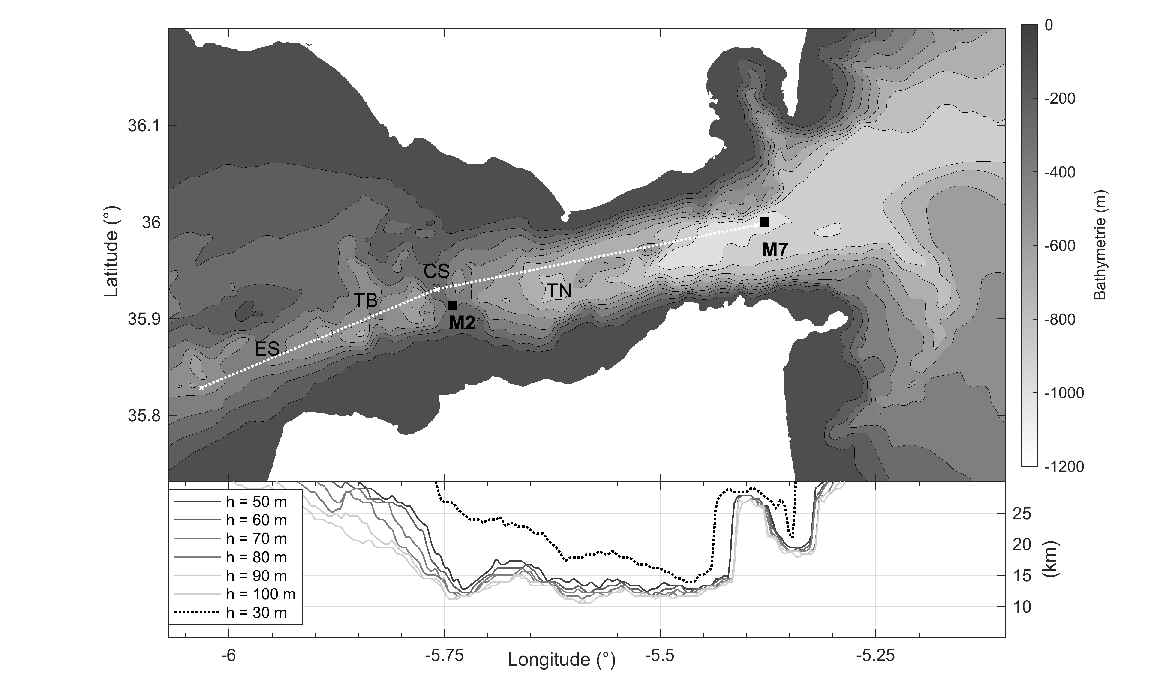
\includegraphics[width=1\textwidth]{./GBR2D/figure2.eps}
 \caption { a) Bathymetry of the strait of Gibraltar, with the section used for the present model configuration (white dotted line). Black squares indicate the position of moorings from \citet{CW90}; ES: Espartel Sill, TB: Tanger Basin, CS: Camarinal Sill , TN: Tarifa Narrows. b) Width of the Gibraltar Strait along transverse direction (y) between 2 isobaths of depth h.}
 \label{Fig1}
\end{figure}

\indent Figure \ref{Fig1}.a presents the 500-m-resolution bathymetry gathered in the framework of the HOMONIM project coordinated by the French Navy (SHOM) and MeteoFrance, and as provided by the French Navy \citep{Biscara2016}. The  main bathymetric features as well as the localization of the studied 2D vertical section are exhibited. This section is chosen as close as possible to the transect of Farmer and Armi's Gibraltar Experiment performed in April 1986 \citep{FA1988} and coincides in the western area with the Mediterranean waters privileged path. Hereafter, $u$ is the velocity in the longitudinal direction of the section and $v$ the velocity in the transverse direction. Figure \ref{Fig1}.b presents the Gibraltar Strait width according to different reference depths. This plot shows that an averaged thirteen kilometer width can be used, featuring steep slopes at the lateral boundaries of the strait, especially in Tarifa Narrows.

Simulations are performed with 50m and 220m horizontal resolutions. The bathymetry used in the simulations is averaged laterally to limit the unrealistic effect of local seamounts in the transverse direction such as those found in TN (which can end up acting as another sill in a 2D vertical section). To that end, a Gaussian interpolation of the bathymetry along the section in Figure \ref{Fig1}.a is used with a greater Gaussian radius in the transverse direction than in the longitudinal direction. The Gaussian radius in the transverse direction is set to 1500 m (i.e. lower than the width of the strait in figure \ref{Fig1}.b). As a consequence, the bathymetry only reflects the deepest areas in the canal. In the longitudinal direction, the Gaussian interpolation radius is set to 300 m to preserve the bathymetry variability in this direction.

The minimum depth thus assessed at Camarinal Sill (i.e. the main sill in the Strait), along the transect's path goes from the value of approximately 200 m to 245 m. The model bathymetry used is the one shown in Figure \ref{scheme_GBR}. A reference simulation (hereafter named \textbf{SimRef}) is carried out at 50-m horizontal resolution with additional characteristics and parameters listed in \ref{tabsimref}.

~

\begin{table}
\caption{Numerical parameters of simulation \textbf{SimRef}}
\centering
\begin{tabular}{|p{0.5\linewidth}|c|c|}
\hline
Number of horizontal points & \multicolumn{2}{c|} {2661x3}  \\
%\hline
Horizontal scale ($\Delta x$) & \multicolumn{2}{c|} {50 m}\\ 
%\hline
Number of vertical $\sigma$-levels & \multicolumn{2}{c|} {40} \\
%\hline
Depth & Min & Max\\
%\cline{2-3}
   & 247 m & 900 m\\
%   \hline
   Vertical scale ($\Delta$z) & 6 m & 23 m\\
%\hline
Slow time step ($t_s$) & \multicolumn{2}{c|} {1 s}\\
%\hline
Fast time step ($t_f$) & \multicolumn{2}{c|} {1/8 s}\\
%\hline
Spin up period & \multicolumn{2}{c|} {72 h}  \\
%
Vertical Viscosity & \multicolumn{2}{c|} {$10^{-6}$ m$^2$/s}\\
%\hline
Lateral Viscosity & \multicolumn{2}{c|} {$10^{-5}$ m$^2$/s}\\
%\hline
Diffusivity & \multicolumn{2}{c|} {$10^{-6}$ m$^2$/s}\\
%\hline
Momentum Advective Scheme & \multicolumn{2}{c|} {TVD - Van Leer}  \\
%\hline
Turbulent Closure Scheme & \multicolumn{2}{c|} {none}  \\
%\hline
T, S Advective Scheme & \multicolumn{2}{c|} {WENO5}  \\
Quadratic bottom drag coefficient & \multicolumn{2}{c|}{$10^{-3}$}\\
Atmospheric forcing/fluxes & \multicolumn{2}{c|}{none}\\
\hline
\end{tabular}
\label{tabsimref}
\end{table}

\begin{figure}[!t]
 \centering
 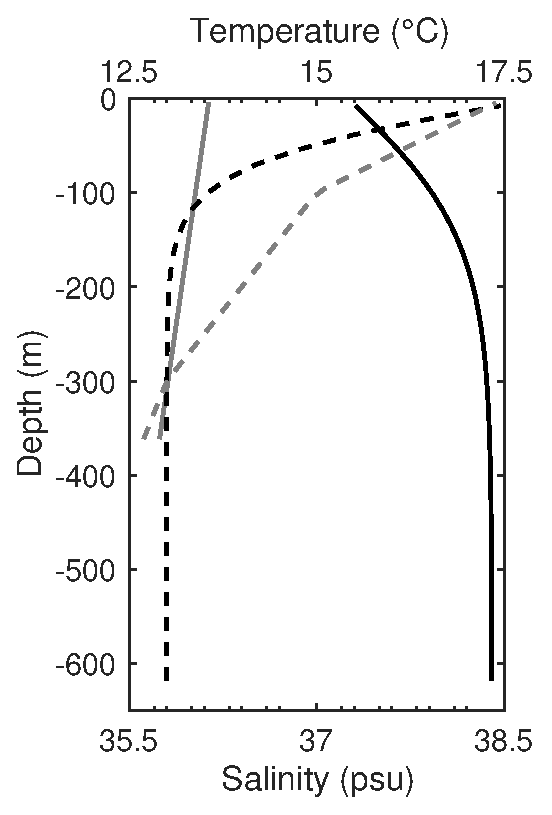
\includegraphics[width=0.5\textwidth]{./GBR2D/figure3.eps}
 \caption{Initial salinity (solid) and temperature (dashed) profiles of Mediterranean water (black) and Atlantic water (grey).}
\label{fig_LEx}
\end{figure}


%--------------------------------
\subsubsection{Initial Water Masses, Tidal Forcing and Boundary Conditions}
\label{init}
%--------------------------------
\indent The temperature and salinity reference profiles are chosen to initialise the density field of the simulations. A minimum of two profiles for each of those variables is needed to initialize gradients associated with sloping isopycnal surfaces in a given direction. According to \citet{Sannino2002}, a lock-exchange initialization is performed with homogeneous Atlantic water initially to the west of the CS and homogeneous Mediterranean water to the east. A three-day spin-up described in Section \ref{Coriolis}) is then performed to set up the exchange flow in the strait.

The initial temperature and salinity profiles are presented in Figure \ref{fig_LEx}. The contrast in salinity between Atlantic and Mediterranean waters is noticeable, with respective mean values of 35.9 and 38.2. 

In the following, the interface between Atlantic and Mediterranean layers is taken as the 37 isohaline, following \citet{Bryden94}. Density is now expressed as an anomaly (written $\rho'$) relative to a reference (mean) density $\rho_{0}$. From now on, the implicit reference density (unless contraindicated) will be $\rho_{0}=1033.7$ kg/m$^3$: a value reached in the pycnocline separating the two water masses.

An idealized M2 tidal forcing (of period T = 12.4 h) is prescribed at the open boundaries after the spin-up period (at t = 3 days = 5.8 T ). It is introduced thanks to a barotropic current of amplitude 0.4 m/s at the western boundary (0.8 m/s at CS), corresponding to a moderate regime according to the TPXO-8 tidal atlas \citep{tpxo8}. Lateral forcing is introduced at the open eastern and western boundaries through mixed active passive radiation conditions  \citep{Marchesiello2001} ; cyclic conditions are imposed to the northern and southern open boundaries.

%----------------------------------------------------------------------------
\subsubsection{Initial Flow and Effect of Coriolis Force}
\label{Coriolis}
%----------------------------------------------------------------------------

The Gibraltar strait lateral boundaries  are distant of about 15 km, with a clear funneling effect from the CS to the eastern end of the strait ( 5.4$^\circ$W; see Figure \ref{Fig1}.b). The internal Rossby radius $R$ (\ref{app_Rossby}) is usually found to vary from 10 to 20 km \citep{Bormans1989, CW90, Vlasenko2009}. The width of the strait and the Rossby radius $R$ being of the same order of magnitude, rotational effects can be neglected as a rather good approximation. Therefore, the momentum balance is mainly between the acceleration and the pressure force in the equation (\ref{momentum}) and the geostrophic adjustment in the along-strait direction is locally neglected. In their observations \citep{FA1988} and the 3D-modeling configurations \citep{Sannino2002}, the consequence of Earth's rotation is a cross-strait shear of along-strait velocity \citep{Bormans1989} and a tilt of the isopycnals: along the southern boundary  (i.e. along the Moroccan coast), the interfacial isopycnal is deeper and the flow reaches larger velocities.

As the transverse flow, the coastal boundaries, and the resulting ``funnelling effect'' cannot be simulated in a 2D vertical section, it is necessary to examine whether completely ignoring rotational effects is viable in a 2D vertical approximation. To that end, three different numerical simulations of the stratification and the mean circulation are compared: (i) one simulation with the Coriolis force activated from start to end (\textbf{SimAllCor}; $f = 8.5 \ 10^{-5} s^{-1}$), (ii) the second one without the Coriolis force (\textbf{SimNoCor}; $f=0$), and (iii) the last one with the Coriolis force activated only after a three days spin-up period (\textbf{SimRef}). Apart from the Coriolis parameter, all the three simulations where performed with the characteristics given in Table \ref{tabsimref} for \textbf{SimRef}. During the very first hours of simulation time, the `Lock-Exchange dam' separating the Atlantic and Mediterranean water-masses disappears; a gravity current is generated with dense Mediterranean waters flowing down the western slope of CS and light Atlantic water spreading in the surface layer east of the sill.

Figure \ref{fig2} presents the field of the longitudinal velocity ($u$) as well as some isopycnals for \textbf{SimAllCor} (a) and \textbf{SimNoCor} (b) at t = 72 h (i.e., the end of the spinup period). The bold isopycnal surface $\rho'= -0.7\ kg/m^3$ corresponds at that time to the 37psu-isohaline. Figures \ref{fig2}.a-b  also present the transverse-velocity ($v$) isotachs $\pm$ 0.5 m/s. Figures \ref{fig2}.c-d show the tidal residual components $u$ and $v$ in the water column at the two dashed vertical lines on figures \ref{fig2}.a-b. These locations correspond to the moorings indicated in Figure 1 of \citet{CW90}. Using the 37psu-isohaline as a frontier between the two water masses, the 3T time-averaged transport through the left dashed line at the CS is given in the columns labelled 'Transport' of the Table \ref{tabdepth}.

In \textbf{SimNoCor} (Figure \ref{fig2}.b), a clear vertical shear of the along-section velocity can be seen between the two water masses. The shear is still featured in the 3T-averaged current profiles of Figure \ref{fig2}.c and is, for station M2, in accordance with the observations given by the moorings at the CS. This shear has decreased since initialization as progressive mixing of the two water masses reduces the baroclinicity. The currents in \textbf{SimAllCor} and \textbf{SimRef} are weaker, with locally negative currents in the upper layer (see Figure \ref{fig2}.c). This is confirmed by the layer-averaged transports presented in Table \ref{tabdepth}, where values in \textbf{SimAllCor} and \textbf{SimRef} are one order of magnitude smaller than in \textbf{SimNoCor}. Using an average strait's width of 13 km, an approximate baroclinic transport for the strait can be estimated from the values in Table \ref{tabdepth}; for \textbf{SimNoCor} it would be of 0.6 Sv: it is slightly weaker than the range of 0.7-1 Sv estimated from various field observations (see a review in \citet{Sammartino2015}). In \textbf{SimAllCor} and \textbf{SimRef}, the cross-section velocity is due to the inclusion of the Coriolis force. More precisely, during the spin-up phase of \textbf{SimAllCor}, the effect of rotation can no more be neglected after 6 hours. At that time, the upper Atlantic layer has spread over a distance of about 26 km and the cross-section velocity featured in Figure \ref{fig2}.a is already significant.

%
%%%%%%%%%%%%
% Figure 
%%%%%%%%%%%%
\begin{figure}
% \centering
 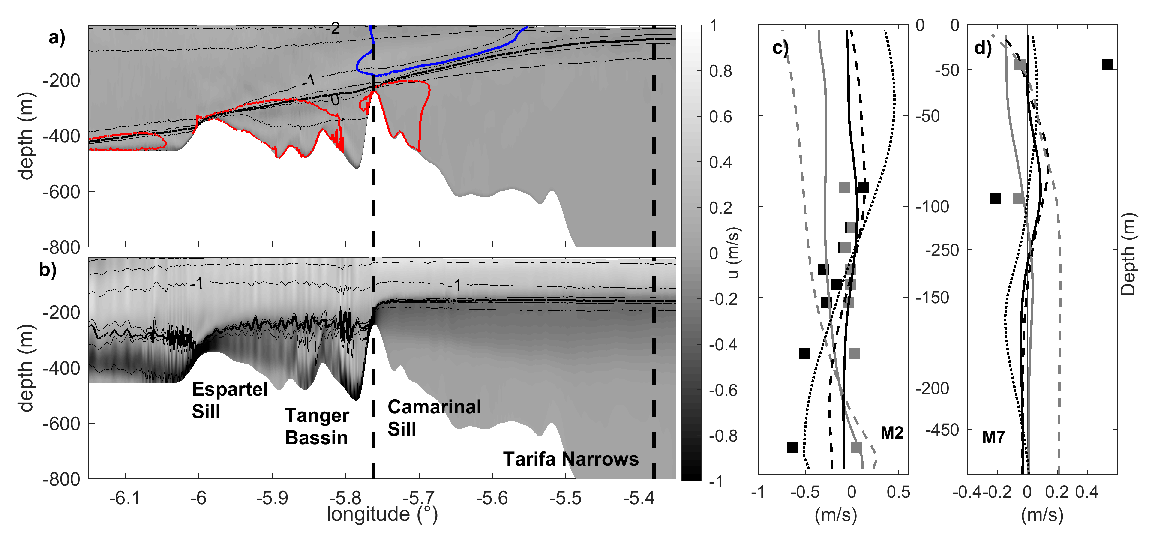
\includegraphics[width=\textwidth]{./GBR2D/figure4.eps}
 \caption {a - b ) Longitudinal currents $u$ (greyscale) and isopycnals (thin black lines) of density anomaly between -2 kg m$^{-3}$ and 0.5 kg m$^{-3}$ with an interval of 0.5 kg m$^{-3}$ at t = 72 h at the end of the spin-up phase for \textbf{SimAllCor} (a) and \textbf{SimNoCor} (b). The bold line is for isopycnal $\rho' = -0.7 \ kg/m^3$. The vertical dashed lines indicate the location of the profiles given in c and d. Color contours in (a) indicate the values of transverse currents $v$. Inside the red contours $v \geq 0.5 \ m/s$, while inside the blue contours $v \leq -0.5 \ m/s$.  
  c - d ) 3T-averaged longitudinal currents (black) and transverse currents (grey) for \textbf{SimRef} (plain), \textbf{SimAllCor} (dashed) and \textbf{SimNoCor} (dotted). Observation of tidal-mean currents at stations M2 and M7 (Fig. \ref{Fig1}) from \citet{CW90} (squares).}
  \label{fig2}
\end{figure}

With no coastal boundaries to hinder the geostrophic adjustment within the strait, the initially longitudinal gravity current is almost completely converted into transverse geostrophic current with spurious (non physical) consequences on the slope of the isopycnals. Geostrophy enables a thermal-wind balance for the transverse $v$ component: 
\begin{equation}  
    \label{Thermal_wind}
    \displaystyle   
	\frac{\partial v}{\partial z}
    =-\frac{g}{\rho_0 f} \frac{\partial \rho}{\partial x}
\end{equation}
This is particularly apparent to the east of the CS in Figure \ref{fig2}.a where the pycnocline is located at the transition between positive and negative transverse velocities. As a consequence, the pycnocline slope is $\Delta z/\Delta x = 6.10^{-3}$ (Table \ref{tabdepth}) and the Atlantic water cannot spread further than the resulting surface front. In \textbf{SimRef}, the Coriolis force is introduced only after a 72-h-spin-up period leading to the state presented in Figure \ref{fig2}.b. In this case, the resulting slope and transverse velocity are smaller than in \textbf{SimAllCor}. %(figure \ref{fig_current}.c). 
The pycnocline in the eastern part of the domain is deeper whereas it is shallower in the western part. However, longitudinal currents remain weak. In contrast, in \textbf{SimNoCor} the thermal-wind balance is not allowed and, away from the sills, $\Delta z/\Delta x$ vanishes. In the longitudinal direction, the main balance is between the pressure force $(-1/\rho_0\  \partial p/\partial x)$ and the acceleration term. In this case, the shear of the longitudinal velocity is better represented at the two moorings. The larger transports in both layers indicate that a larger amount of Mediterranean water enters the Tangier basin than in \textbf{SimAllCor}. This is confirmed by the stratification (Figure \ref{fig2}.a and Table \ref{tabdepth}) since the pycnocline is shallower over the Espartel Sill (and deeper within the TN).

A perfect balance between the transports in the upper and lower layers is not achieved in any of these three numerical experiments. While there is no numerical challenge in achieving longer simulation, the fluxes of Mediterranean and Atlantic waters are not realistically specified to re-stratify properly the water column in these academic configurations. After the spin-up period, the intense tidal mixing and other dissipative processes may end up homogenizing the initial water masses. The gap between the transports in the upper and lower layers disappears as the depth-averaged absolute transports decrease. This process is faster in \textbf{SimNoCor} than in the other configurations in which the thermal-wind balance maintains the isopycnal slopes. In this case, the depth of the 37 psu-isohaline, taken as a moving average over one tidal period at x = $5.4^\circ$W, increases from 130 to 175 m in \textbf{SimNoCor} over three tidal periods (not shown). This impacts the large-amplitude internal waves propagation.

The difficulty to obtain both realistic ambient stratification and circulation is a limitation of the restriction to a 2D vertical section of the dynamical problem targeted. In the proposed implementation, an initial state is obtained by lock-exchange with a spin-up period of 72 h dedicated to the adjustment of the gravity current produced by the 'dam break'. For the remainder of this paper, the reference simulation (\textbf{SimRef}) is chosen as the simulation whose adjustment is made in a non-rotating framework. This initial state has a correct mean exchange but it is weakened as the tidal forcing is introduced and changes the stratification conditions.

To mitigate this problem, the rotation is restored at the end of the spin-up period: the geostrophic balance that ensues stabilizes the slopes of isopycnals by generating a transverse current. The mean exchange is nevertheless reduced but the stratification (i.e. both the slope of the isopycnals and the vertical density gradient) thus saved is crucial to the generation and propagation of the large-amplitude solitary waves. Furthermore, the small-scale processes discussed hereafter take place during the tidal cycle. At this time-scale, the barotropic exchange is dominated by the tidal currents, so that in the reference simulation, the amplitude of the baroclinic exchange is correct. Note that if rotation is activated from the beginning of the spin-up period (\textbf{SimAllCor}), it leads to unrealistically-large slopes of the isopycnals (see Table \ref{tabdepth}). 


%%%%%%%%%%%%%%%%%%%%%%%%%%%%%%%%%%%%%%%%%%%%%%%%%%%%%%%%%%%%%%%%%%%%%%%%%%%%%
\subsection{The Reference Simulation}
\label{sRef}
%%%%%%%%%%%%%%%%%%%%%%%%%%%%%%%%%%%%%%%%%%%%%%%%%%%%%%%%%%%%%%%%%%%%%%%%%%%%%

\indent The reference simulation presented previously is now evaluated thanks to the observational data from the Gibraltar Experiment \citep{FA1988}. We describe the hydraulic controls, the primary instabilities and the dynamics of the ISW in this reference simulation.

%----------------------------------------------------------------------------
\subsubsection{Comparison with \textit{in situ} Observations}
\label{refobs}
%----------------------------------------------------------------------------

\indent In the present section, observations from the Gibraltar Experiment \citep{FA1988} are investigated in order to evaluate the quality of the model solution obtained with the reference configuration \textbf{SimRef}.

The table \ref{tabdepth} presents the pycnocline depth and slope at different locations along the section for the three configurations and the observational data. The depth and slope for \textbf{SimAllCor} and \textbf{SimNoCor} are calculated after 72 h of simulation and correspond to the isopycnal surface $\rho'$= -0.7 kg/m$^3$ in figures \ref{fig2}.a-b, whereas for configuration \textbf{SimRef} the same isopycnal taken in a 3T-averaged stratification corresponding to Figure \ref{fig_fn_ref}. In \textbf{SimAllCor}, the isopycnals have a greater slope than the reported observations from Gibraltar Experiment (0.006 vs 0.003). In \textbf{SimNoCor}, there is no slope away from the sills, while as discussed before, the slope obtained in \textbf{SimRef} is small. The stratification in \textbf{SimRef} is close to that of \textbf{SimNoCor} in the eastern part with an isopycnal close to the horizontal. In the western part and over the CS, the pycnocline is shallower than in the other two simulations (Table \ref{tabdepth}).

In the following, we further investigate small-scale dynamical processes such as hydraulic jump and ISW propagation in configuration \textbf{SimRef}. This is also the baseline configuration used to perform all sensitivity tests presented hereafter.

%%%%%%%%%%%%
% Table 
%%%%%%%%%%%%
\begin{table}[!h]
 \caption{3T time-averaged transports (m$^2$/s) at CS, depth (m) and slope of the interface.}
 \centering
  %\begin{tabular}{|l|c|c||c|c|c||c|c|}
  \begin{tabular}{|p{0.2\linewidth}|p{0.1\linewidth}|p{0.1\linewidth}||p{0.1\linewidth}|p{0.1\linewidth}|p{0.1\linewidth}||p{0.09\linewidth}|p{0.09\linewidth}|}
 \hline
 &\multicolumn{2}{c||}{Transport (m$^2$/s)} & \multicolumn{3}{c||}{Pycnocline Depth (m)} & \multicolumn{2}{c|}{Pycnocline Slope}\\
  \hline
   &Upper  & Lower & ES & CS & TN& ES-CS & CS-TN\\
    &layer &layer &(5.91$^\circ$W)&(5.71$^\circ$W)&(5.52$^\circ$W)& & \\
   \hline
   \citet{FA1988} & / & / & 190  & 125 & 60 & 0.003 & 0.003\\
   \hline
   \textbf{SimAllCor} & -5 & -13 & 300 & 175 & 70 & 0.006 & 0.006\\
   \hline
   \textbf{SimNoCor} & 50 & -45 & 290  & 200 & 220& 0.005 & -0.001\\
   \hline
   \textbf{SimRef} & 0.7& -6 & 245 & 175 & 160 & 0.004 & 0.001\\
  \hline
 \end{tabular}
 \label{tabdepth}
\end{table}

%%%%%%%%%%%%%%%%%%%%%%%%%%%%%%%%%%%%%%%%%%%%%%%%%%%%%%%%%%%%%%%%%%%%%%%%%
\subsubsection{Tidal Currents \& Hydraulic Control.}
\label{tide_hyd}
%%%%%%%%%%%%%%%%%%%%%%%%%%%%%%%%%%%%%%%%%%%%%%%%%%%%%%%%%%%%%%%%%%%%%%%
\begin{figure}[!h]
\centering
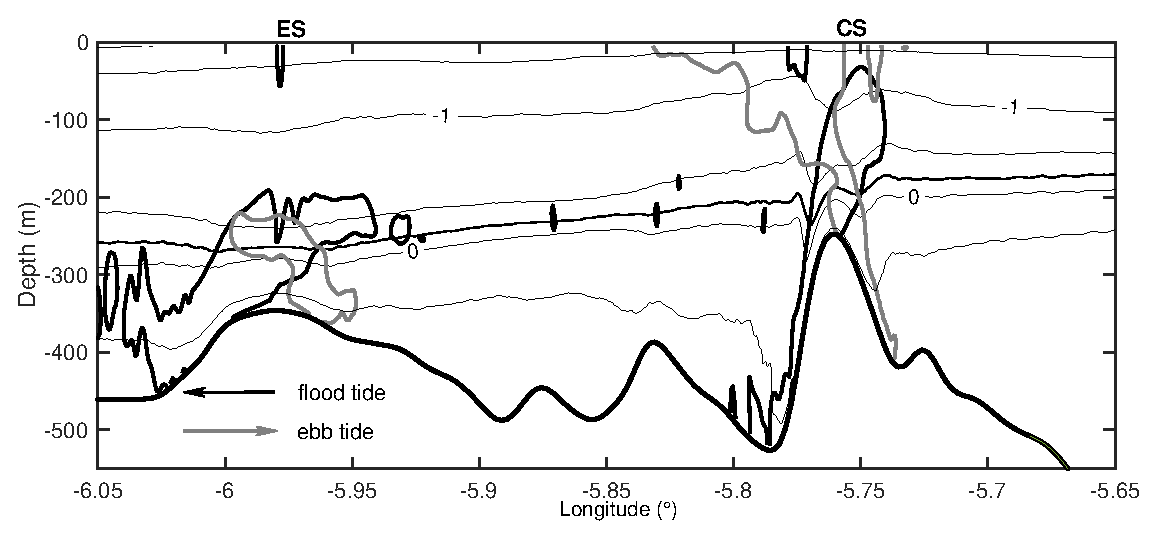
\includegraphics[width=1\linewidth]{./GBR2D/figure5.eps}
\caption{ Isopycnal position averaged over a 3T time interval in \textbf{SimRef} (thin black lines are density anomaly contours between -1.5 kg m$^{-3}$ and 0.5 kg m$^{-3}$ with an interval of 0.5 kg m$^{-3}$;  
%the bold line shows $\rho'$ = -0.7 kg/m$^3$). 
Thick black (grey) contours indicate critical Froud number $F=1$ during flood (ebb) tide, inside which the flow is supercritical.}
\label{fig_fn_ref}
\end{figure}


In the present study, the Froude number ($F$) is simply defined at each grid point as the ratio between the local longitudinal velocity $u$ and the theoretical speed $c_1$ of the first internal wave mode, computed with the modal decomposition for each point of the x-axis (see \ref{app_Froude} for details).

For single-layer flows, hydraulic control occurs in the region of transition between subcritical and supercritical flows. In this region, the condition $F>1$ is met over the whole water column. For multi-layer flows, the Froude number condition may be satisfied in a few layers only. In this case, the layers where the flow becomes supercritical are considered as "hydraulically controlled".

Three areas of potential hydraulic control in Gibraltar Strait are identified from previous studies: the CS, the ES and the narrowest part of the TN (near 5.5$^\circ$W longitude in figure \ref{Fig1}). \citet{FA1988} found persistent controls for first internal wave mode at the ES, the CS and the TN. \citet{Sannino2009b} found only ephemeral appearances of such controls, except at the ES where it is permanent. The discrepancy is likely lying in the definition and the estimation of the composite Froude number.

Figure \ref{fig_fn_ref} shows the regions where the flow is critical. Closed contours indicate the locations of critical Froude number ($F=1$), inside which the flow is supercritical. The longitudinal velocity fields ($u$) used to estimate F are taken at maximum outflow (grey) at $t = 7.5\ T$ and maximum inflow (black) at $t = 8\ T$. The internal waves phase speed $c_1$ is computed from the 3T-time-averaged stratification represented in Figure \ref{fig_fn_ref}. No control of the first mode is ever seen in TN : this is a consequence of the 2D simplification which excludes the representation of the tidal flow intensification by the narrowing of the strait at TN. On the other hand, hydraulic control is expected at both sills. The location where it should occur alternate between the eastern (during ebb) and western (during flood) sides of the sills, with a return to subcritical flow when tidal current slackens. The Froude number easily goes beyond 2 in the Mediterranean outflow at CS, where the flow is supercritical through most of the water column, except sometime at the surface. At ES, the lower layer may become supercritical with Froude number that never exceeds 1.5. The lack of persistent control at ES may be a consequence of the crudely imposed stratification.

%-----------------------------------------------------------------
\subsubsection{Primary Instabilities in the Hydraulic Jump Area}
\label{sinsta}
%-------------------------------------------------------------------

\begin{figure}[!h]
\centering
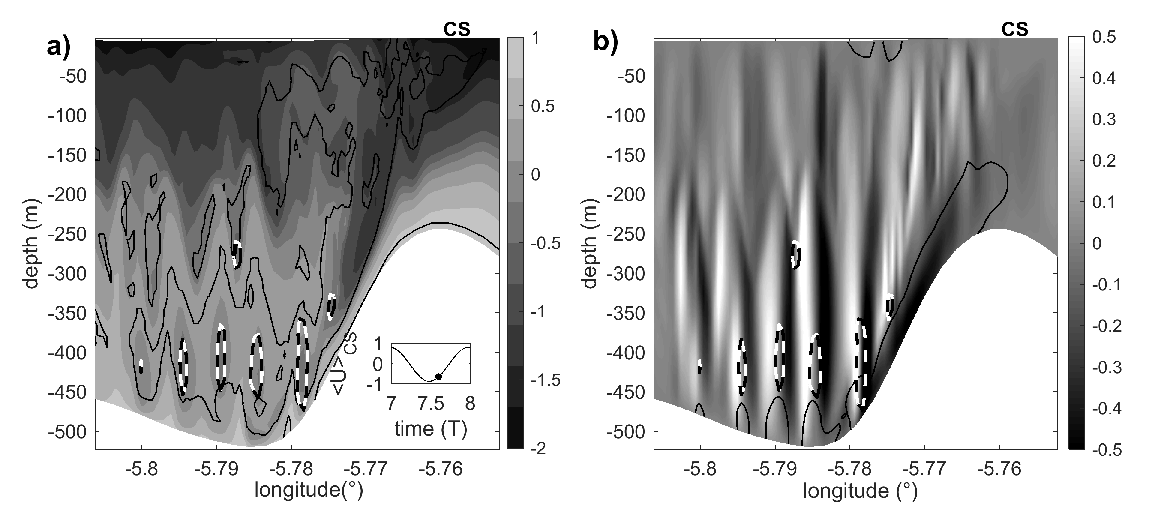
\includegraphics[width=1\linewidth]{./GBR2D/figure6.eps}
	\caption{a) Density anomaly (greyscale ; $kg/m^3$) in the lee side of Camarinal Sill in \textbf{SimRef} at t = 7.56 T. Black contours indicate the location where the Richardson number is  0.25. b) Vertical velocity (greyscale ; $m/s$) in the lee side of Camarinal Sill in \textbf{SimRef} at t = 7.56 T. The black contour indicates the location where the Froude number is 1. a) and b) The black and white contour represents $OW=-4*10^{-4}\ s^{-2} $.} 
\label{RH_CS}
\end{figure}

One manifestation of the hydraulic control is the formation of hydraulic jumps in specific regions where the flow transitions from supercritical to subcritical. This is a complex area with steep slopes and high shears where flow-topography interaction can generate small-scale coherent structures. The largest ones are resolved in \textbf{SimRef} and are characterised here with various methods. First, the Okubo-Weiss parameter (\ref{annexeOW}) is computed to investigate the presence of new 'coherent structures' in the hydraulic jump area. Their dynamics are further investigated using Empirical Orthogonal Functions (EOFs) computed with a Singular Value Decomposition (SVD). Their typical length and velocity scales are finally compared with the expected analytical values of shear instabilities and lee waves.

The dynamics of the CS hydraulic jump are illustrated in Figure \ref{RH_CS}, in which the density field (Fig. \ref{RH_CS}.a) and the vertical velocity field (Fig. \ref{RH_CS}.b) over the western slope of the CS are represented during flood. Several flow parameters were also computed and are depicted in Figure \ref{RH_CS}.a and b. These parameters are :

\begin{enumerate}

\item
The Froude number defined in \ref{app_Froude}. The contours of critical Froude number $F=1$ are shown in Figure \ref{RH_CS}.b, inside which the flow is supercritical.

\item
The Richardson gradient number defined as $Ri =  N^2 / \left({\partial u}/{\partial z}\right)^2$, with $N$ the Brunt-V\"ais\"al\"a frequency defined in Eq.\ref{eqN}. Contours of $Ri = 0.25$ are depicted in Figure \ref{RH_CS}.a, as $Ri<0.25$ is a required condition for the development of shear instabilities.

\begin{equation}
N=\sqrt{ - \frac{g}{\rho_0} \frac{\partial \rho}{\partial z}}
\label{eqN}
\end{equation}

\item
The Okubo-Weiss parameter defined in \ref{annexeOW}. Negative values of OW indicate vortical circulation, and so contours of $OW = -4*10^{-4}\ s^{-2}$ are shown in both Figure \ref{RH_CS}.a and b. 

\end{enumerate}

In Figure \ref{RH_CS}.b, the supercritical flow region (F $>$ 1)  follows the slope of the sill where the velocity in the Mediterranean outflow is larger than 2 m/s (see the contour F = 1 running approximately parallel to isopycnals between 5.76$^\circ$W and 5.77$^\circ$W). At 5.77$^\circ$W, the density field in Figure \ref{RH_CS}.a shows a sharp transition (e.g., isopycnal $\rho'=-0.5kg/m^3$ rises from 350 to 225 m depth), and forms a wedge-shaped region over the supercritical Mediterranean outflow. This is the signature of an internal hydraulic jump. 

Downstream of the hydraulic jump, several small-scale structures are visible. Figure \ref{RH_CS}.a shows patches of lighter water (billows) associated with areas of negative OW values at a depth of 400 m, and large-amplitude disturbances of isopycnals at 150 m. Negative OW values are also located at troughs and can reach $OW=-4*10^{-4} s^{-2} $. Both types of structures are propagating westward and are quite probably shed from the internal hydraulic jump at the tip of the wedge-shaped region at 5.773$^\circ$W, with the size of billows growing rapidly as they travel down-slope. In the potential generation area, Richardson number values are less than 0.25, indicating favorable conditions for generation of primary shear instabilities. 

Further identification of the simulated new features of Figure \ref{RH_CS} is achieved by proceeding with a complex singular value decomposition (SVD) \citep{Pairaud2005} of the velocity field $(w+iu)$ in the water column between 5.795$^\circ$W and 5.78$^\circ$W longitude, during outflow conditions. This region is highlighted in Figure \ref{eof_insta}.a, in which the time mean field of longitudinal velocity $u$ is presented, showing the intense outflow below layers of lesser velocities. The mean density field and location of $Ri\ <\ 0.25$ are also indicated, the former showing a homogeneous area between 50-150 m above the seafloor. The SVD gives a first singular vector responsible for $28\ \%$ of the total variance corresponding to the evolution of the barotropic forcing (not shown). The remaining singular eigenvectors have lesser corresponding variance and show smaller structures with high-frequency variations in the singular right eigenvector. Two consecutive singular vectors often have very close eigenvalues and temporal variations.

\begin{figure}[!h]
\centering
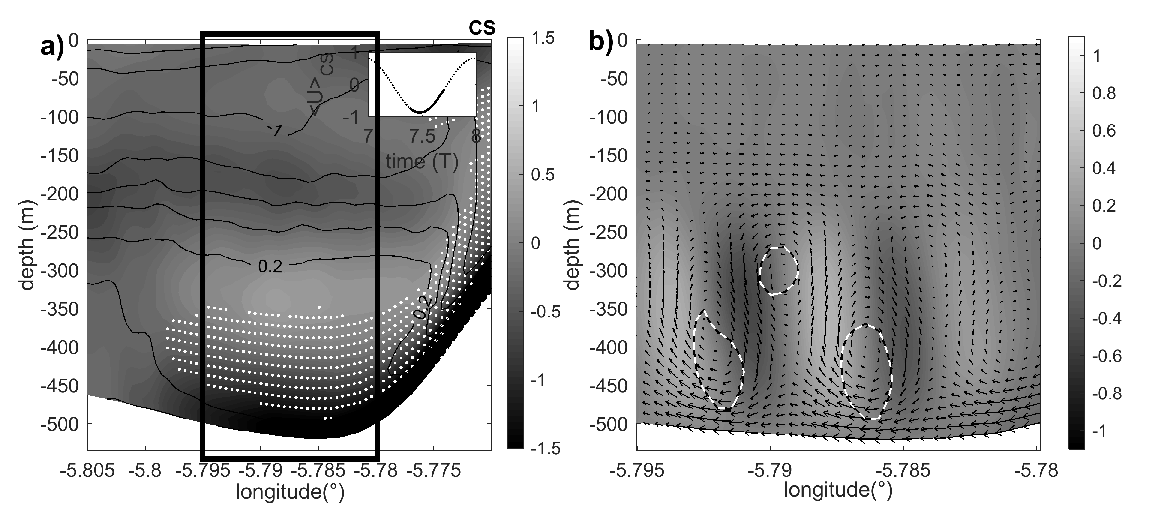
\includegraphics[width=1\linewidth]{./GBR2D/figure7.eps}
 \caption {a) Mean field of longitudinal velocity $u$ (m/s) ; greyscale) and isopycnals (black lines, density anomaly between -1.6 kg m$^{-3}$ and 0.5 kg m$^{-3}$ with an interval of 0.3 kg m$^{-3}$ ) with location of Ri$<$0.25 (white dots). b) Vertical velocity $w$ (greyscale ; m/s) and velocity vectors of the superposition of the second and third singular vectors of the SVD decomposition added to the mean velocity field of (a). Black and white contours are OW=$ -1.5*10^{-4}\ s^{-2}$}
 \label{eof_insta}
\end{figure}

Figure \ref{eof_insta}.b shows the reconstructed field of the combination of the second and third singular vectors (respectively responsible for $13\ \%$ and $11\ \%$ of total variance) added to the mean field shown in Figure \ref{eof_insta}.a. The Okubo-Weiss parameter is again computed for the resulting velocity field, which shows two rows of y-axis vortices centered at z = -300 m (anti clockwise) and -400 m (clockwise). The upper row of vortices appears to generate the observed interface oscillations.

Based on OW$=$0 contours, the lower clockwise vortices have an estimated horizontal scale of 200 m and a vertical scale of 150 m, corresponding to horizontal and vertical wavenumbers 3.10$^{-2}$ and 4.10$^{-2}$ m$^{-1}$ respectively. Their propagation speed can be estimated as -0.7 m/s by following the center of the billows defined by areas of negative OW values. The distance between the centers of two consecutive vortices is L = 530 m. The centers of the upper anti-clockwise and lower clockwise vortices are shifted along flow by L/2, so that the extrema of their respective vertical velocities are aligned vertically. It seems that a transfer of momentum occurs between the two rows of vortices in a way reminiscent of the Vallis model of edge waves in a stratified region of a shear flow (pp 254-258 in \citet{Vallis2006}). 

The length scales deduced from this SVD analysis can now be compared with expected scales from simple analytical models for shear instabilities and internal waves based on the general characteristics of the flow on the western slope of Camarinal.

Shear flow instability in a two-layer system of infinite depth results in a mixed interface of vertical extent $\Delta H$ expressed by equation 14.6 of \citet{Cushman-RoisinBenoit2011} :
%
\begin{equation}
\Delta H \approx \frac{1}{k_{min}} = \frac{\rho_0 (u_1 - u_2)^2}{2(\rho_2-\rho_1)g}
\end{equation}
%
with $k_{min}$ the wave-number of the most unstable mode in this system, taken as the scale of the primary instability that will develop. In the generation area of CS, $(u_1-u_2)$ is in the range of 1.2 to 2 m/s and $(\rho_2-\rho_1)$ is in the range of 1.2 to 1.7 kg/m$^3$. Additional values are $\rho_0$ = 1033.7 kg/m$^3$ and g = 9.81 m$^2$/s. This gives a range of vertical scales between 44 m and 183 m and $k_{min}$ between 2.10$^{-2}\ m^{-1}$ and 5.10$^{-3}\ m^{-1}$. The scales of the simulated lower row of vortices are in the upper part of this range.

Lee waves are another candidate for small-scale transient flow and the interfacial oscillations observed in our solutions. Their generation over topography is expected when tidal excursion is larger that the topographic length scale $1/k_b$, i.e, $k_b u_0/\omega > 1$ \citep{StLaurent2002}. The slopes of Camarinal Sill are not symmetrical, as can be seen for example in Figure \ref{fig2}. On the western side of the sill, the depth increases from 250 m (at 5.76$^\circ$W) to 510 m (at 5.78$^\circ$W) over only 1.8 km, whereas on the eastern side it increases from 250 m to 620 m (at 5.65$^\circ$W) over 9.4 km. $k_b$ is thus chosen in a range between $3.10^{-3}\ m^{-1}$ and $6.10^{-4}\ m^{-1}$. $u_0=0.4\ m/s$ is the amplitude of the barotropic tidal current away from the sill. In these conditions, the ratio $k_b u_0/\omega$ ranges between 1.7 (over the west slope) and 8.9 (over the east slope). Based on this, we cannot rule out the possibility that lee waves are generated over the CS.

If the simulated small-scale structures would originate from lee waves, their phase speed would be comparable to a mode-1 internal gravity waves. This can be estimated using the same method as in \ref{app_Froude} for the average stratification presented in Figure \ref{eof_insta}.a. It yields a value of 1.4 m/s in the area down-flow of the hydraulic jump, which is twice the estimated propagation speed of both rows of simulated structures. Therefore, even though lee-wave generation is theoretically possible, the interfacial oscillations observed in the simulation appear more consistent with the stirring effect of the bottom coherent vortices, whose scales fall within the range of expected values for KH instability.

We conclude that coherent structures are clearly identified in our simulations. They are generated in an area of potentially unstable shear $(Ri\ <\ 0.25)$ and are associated with billows of lighter mixed fluid. The deeper row of vortices can reasonably be interpreted as Kelvin-Helmholtz primary instabilities. Their downstream behaviour further corresponds to a 2D pairing of two consecutive Kelvin-Helmholtz billows. These billows are advected in a region of westward flow between the Mediterranean vein and  Atlantic waters up until 5.8$^\circ$W. At this location, advection is reduced as the lower layer decelerates and the billows are uplifted in a flow recirculation and mixed in the pycnocline.
These small-scale features appear in the simulation for as long as the hydraulic jump is present, injecting water from the pycnocline in the outflow and vigorously mixing the Atlantic and Mediterranean waters until the tidal currents weaken sufficiently for the flow to become subcritical. 

 However, the dynamics simulated in a 2D vertical section with no transverse flow and no transverse instability may differ from the real ocean. In a fully 3D configuration, primary Kelvin-Helmholtz instabilities should decay faster as secondary Kelvin-Helmholtz instabilities develop along the transverse rotation axis of the primary billows. This is precluded in the present 2D configuration, even with enhanced resolution, as only y-axis billows can occur.

\citet{Wesson94} observed billow structures in the area of CS with an extension of several tens of meters. This length scale is much smaller than the one simulated in the present numerical configuration. However, these observations were made in shallower regions, i.e. probably closer to the generation area: larger billows more in line with those simulated in the present study could thus develop downstream. Further observations on site are needed, although short length-scales and fast propagation speed would require adapted measurement strategies.

%------------------------------------
\subsubsection{Internal Tide Dynamics}
\label{sisw}
%------------------------------------

\begin{figure}[!h]
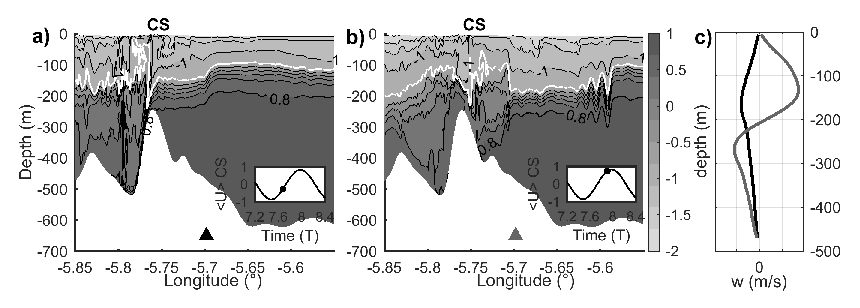
\includegraphics[width=\textwidth]{./GBR2D/figure8.eps}
  \caption{Density anomaly fields ($\rho$ ; $kg/m^3$) of \textbf{SimRef} zoomed over CS at t = 7.7 T (a) and t = 7.9 T (b). The position of $\rho'\ =-0.7\ kg/m^3$ isopycnal is shown in white. c) Profiles of vertical velocity at the position marked by a triangle in (a)-black and (b)-grey.}
  \label{fig_gen_CS}
  \end{figure}
  
\begin{figure}[!t]
\centering
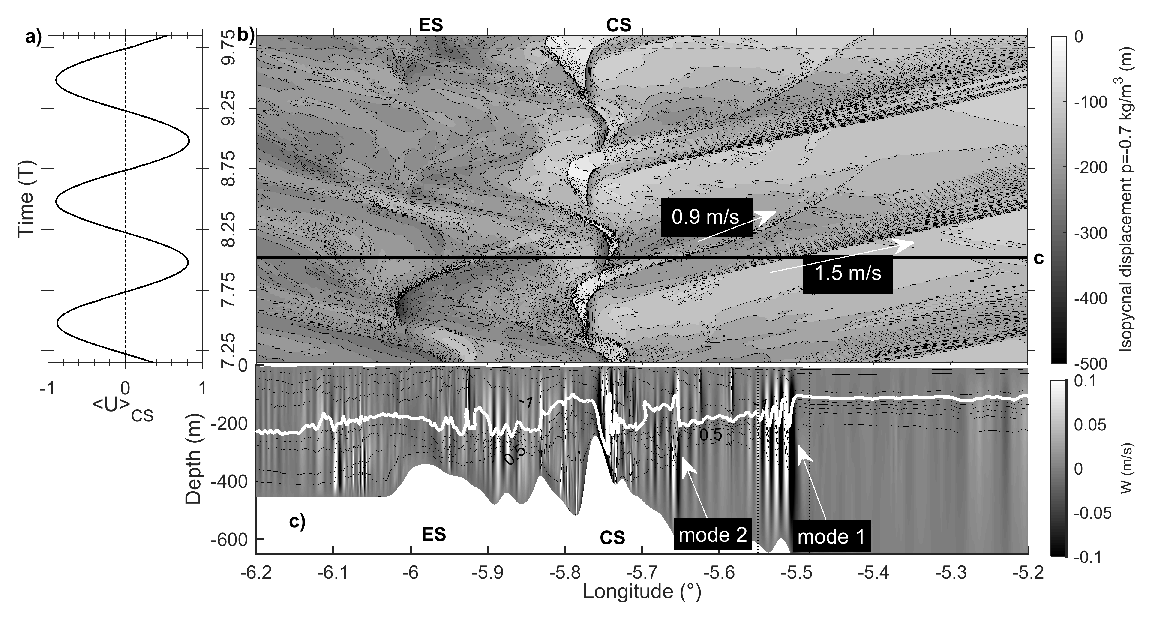
\includegraphics[width=1\linewidth]{./GBR2D/figure9.eps}
 \caption {(a) Depth-averaged currents over CS. (b) Space-time diagram of the vertical displacement of isopycnal $\rho' = -0.7\ kg/m^3$ of \textbf{SimRef} ($\Delta z = 50\ m$ between two contours). The black line indicates the time used in the bottom panel. (c) vertical velocity field (greyscale) and isopycnals (black lines ; density anomaly between -1.9 kg m$^{-3}$ and 0.5 kg m$^{-3}$ with an interval of 0.3 kg m$^{-3}$ ) at the time indicated in panel (b). In white is the isopycnal $\rho' = -0.7\ kg/m^3 $.}
 \label{hov_ref}
\end{figure}

In \textbf{SimRef}, two main types of large amplitude wave propagating eastward can be observed. Both of them are generated at CS while tidal currents reverse from westward to eastward. This is illustrated in Figure \ref{fig_gen_CS}.a-b. First, a mode-1 wave appears as a bore over the sill's crest approximately 2.25 hours after the westward flow peaks. 
In Figure \ref{fig_gen_CS}.a, it has propagated over the eastern slope of the sill's crest and is now at 5.7$^\circ$W longitude: the corresponding profile in Figure \ref{fig_gen_CS}.c has only one maximum as expected for a mode-1 internal wave. This wave rapidly steepens while a hydraulic control is maintained on the western side of the sill with lower values of the Froude number. One hour and 15 minutes later, the flow becomes subcritical and a large-amplitude mode-2 wave crosses the sill. 
In Figure \ref{fig_gen_CS}.b, this new wave is propagating over the eastern slope of the sill; its vertical velocity profile is presented in Figure \ref{fig_gen_CS}.c. It exhibits two maxima of opposite signs and a zero-crossing at the pycnocline's depth as expected for a mode-2 internal wave. Additionally, it can be seen in this figure that the bore-like wave has evolved into a train of internal solitary waves, whose propagation is discussed bellow. 

The propagation of internal waves can be characterized by plotting a space-time evolution of a particular isopycnal. In Figure \ref{hov_ref}.b, the depth evolution of the $-0.7\  kg/m^3$ isopycnal is represented (also in a white contour in Fig. \ref{fig_gen_CS}). Regions of sharp horizontal density gradients can be identified periodically in the region of the CS next to 5.76$^\circ$W longitude. They correspond to the generation of hydraulic jumps. The propagation of internal waves are identified by the tilt of isolines, whose slopes provide an estimate of wave propagation speed. There are differences from one tidal cycle to the next because mixing progressively changes the background stratification in the domain. In the following, we focus on the tidal cycle $t\ =\ 7.5\ T\ -\ 8.5\ T$ (second cycle after the end of the spin-up phase), for which the three-tidal-cycle averaged velocity shear and stratification are shown in Figures \ref{fig2} and \ref{fig_fn_ref}.

The mode-1 bore of Figure \ref{fig_gen_CS}.a propagates down-slope of the CS into the TN, where it experiences a transition into a train of solitary waves moving at a speed of 1.5 m/s. In Figure \ref{hov_ref}.c, such a train made of four mode-1 waves can be seen at 5.5$^\circ$W longitude. The amplitude of the first wave reaches 100 m. The solitons train amplitude momentarily increases and exceeds 150 m as it propagates over the slope near 5.5$^\circ$W longitude in the TN (still during ebb tide). From then on, the wave amplitude decreases as it propagates towards the deeper region. Meanwhile the dispersion increases the number of waves as well as their wavelength as noticed in the space-time diagram which shows the envelop of the train of solitons expanding while it propagates eastward. The dispersion as simulated in CROCO is compared with the Korteweig deVries model in \ref{KdVpart}.

Similarly, the mode-2 wave shown in Figure \ref{fig_gen_CS}.b propagates through the shallowest part of the TN at a speed of 0.9 m/s as a new hydraulic jump is being generated over the eastern slope of CS. It is located at 5.65$^\circ$W longitude in Figure \ref{hov_ref}.c, with an amplitude of approximately 100 m. The propagation speed of this mode-2 internal wave subsequently decreases when it reaches the deepest part of the domain while simultaneously the tidal phase shifts to flood. The amplitude of these waves is simultaneously strongly reduced.

The signatures of other large-amplitude internal waves can be seen propagating to the west of the CS in Figure \ref{hov_ref}.b. They are mode-1 and mode-2 internal waves with amplitude in the tens of meters, i.e. smaller than the eastward propagating wave. They are generated when tidal currents switch from eastward to westward in the same fashion as previously described for the wave train produced east of the CS (as tidal currents reverse from westward to eastward).

As discussed in Section \ref{tide_hyd}, a hydraulic control also occurs at the ES. Figure \ref{hov_ref}.b shows the same variations of  isopycnal depth in this area as near the CS during the tidal cycle $t\ \in [\ 7.5\ T,\ 8.5\ T\ ]$, but not on the following cycle anymore. In the latter case, the computed Froude number does not exceed 0.7, as opposed to previous cycles ($t\ \in[\ 6.5\ T,\ 7.5\ T\ ]$ and $t\ \in[\ 7.5\ T,\ 8.5\ T\ ]$) or later ones ($t\ \in[\ 9.5\ T,\ 10.5\ T\ ]$ and  $t\ \in[\ 10.5\ T,\ 11.5\ T\ ]$). In these cases, the variations are similar and hydraulic control occurs at ES. The sequence is as in CS, with a hydraulic control briefly lost at the barotropic flow reversal. Then internal mode-1 waves of 50-m amplitude at a depth of 300 m are released and propagate toward the CS. In Figure \ref{hov_ref}.c, a mode-1 wave can be found at 5.87$^\circ$W. These waves dissipate in the area near the sill as the absolute value of the barotropic current decreases.

In Figure \ref{hov_ref}.c, two vertical lines are drawn in the TN. They refer to measurements made by \citet{FA1988}: the lines indicate the first two baroclinic modes locations three and a half hours after high tide. The right-hand vertical line corresponds to a mode-1 wave and is in agreement with the simulation. However, in \textbf{SimRef}, the distance between the two modes is twice as large as in the observations. Based on observed wave arrivals at various stations, \citet{FA1988} estimated the propagation speed of both mode-1 and mode-2 waves at about 1 to 2.5 m/s for mode 1 and 1 to 1.5 m/s for mode 2. The wave train they observed contained two to three large-amplitude waves, the first one having an amplitude of 100 m. Additional observations by \citet{SG2008} in the TN region give a propagation speed for mode-1 waves ranging in 1.2 m/s and 2 m/s with a large variation in the velocity of two consecutive wave trains due to the weight of the tidal diurnal inequality (K1 and O1).

The mode-1 dynamics simulated in \textbf{SimRef} are consistent with these observations reported by \citet{FA1988} in terms of propagation speed and longitudinal position. However, the simulated mode-2 wave seems too slow and its amplitude too large. Its slower propagation might be due to an underestimation of the barotropic flow that carries the mode-2 within the TN as our 2D vertical approach does not catch well the tunneling effects of this narrowing. This would not affect the mode-1 wave as much, because its linear propagation speed is more intense and the barotropic current advection becomes comparatively small.

The brief hydraulic control loss observed when the tidal currents reverse does not reflect the quasi-permanent control thought to be taking place at ES. In this case, no internal waves packet can be emitted from the ES.


%%%%%%%%%%%%%%%%%%%%%%%%%%%%%%%%%%%%%%%%%%%%%%%%%%%%%%%%%%%%%%%%%%%%%%%%%%%%%
\subsection{Sensitivity Testing}
%%%%%%%%%%%%%%%%%%%%%%%%%%%%%%%%%%%%%%%%%%%%%%%%%%%%%%%%%%%%%%%%%%%%%%%%%%%%%

The reference configuration presented in the previous section is based on several physical and numerical choices which are now investigated ; mostly the impact of the forcing amplitude, momentum balance (hydrostatic approximation) and numerical parameters (spatial resolution, advection schemes). 

%----------------------------------------------------------------------------
\subsubsection{Tidal regime}
\label{TestAmp}
%----------------------------------------------------------------------------

An additional simulation, \textbf{SimS}, is first performed similarly to \textbf{SimRef} changing only the tidal forcing amplitude. The imposed tidal current amplitude at the western boundary is now increased up to 0.6 m/s, so that it reaches 1.3 m/s over the CS. This corresponds to a spring-tide regime.

Figure \ref{fig_cv_spring} presents a comparison between \textbf{SimS} and \textbf{SimRef}. In Figure \ref{fig_cv_spring}.a, the contours of supercritical regions ($F\ >\ 1$) show the the CS hydraulic jump extends further east in \textbf{SimS}. As a result, a mode-1 disturbance (denoted "a" in Figure \ref{fig_cv_spring}.a) is trapped at 5.725$^\circ$W longitude. It propagates eastward when the flow becomes subcritical but the faster bore that is crossing the CS can rapidly catch it up. The outflowing Mediterranean water vein on the westward side of the sill is also thicker in \textbf{SimS} and so is the supercritical area. In addition, a new supercritical region appears on the western slope of a secondary relief at 5.83$^\circ$W longitude (denoted "b" in Figure \ref{fig_cv_spring}.a) with trailing lee waves.

the figure \ref{fig_cv_spring}.b shows an eastward propagating mode-1 solitons packet. Since the initial stratifications are similar, linear phase velocities are the same in \textbf{SimRef} and \textbf{SimS} at the begining. The amplitude of the first trough of the train is 50-m larger in \textbf{SimS} than in \textbf{SimRef}. This should result in increased propagation speed of the solitons in \textbf{SimS}, in contradiction with a slower propagation seen in Figure \ref{fig_cv_spring}.b. It can be explained by the stronger tidal currents advection in the opposite direction in \textbf{SimS}. A mode-2 wave is also generated in both \textbf{SimS} and \textbf{SimRef}, but is only visible in \textbf{SimRef} in Figure \ref{fig_cv_spring}.b as it quickly dissipates in \textbf{SimS} due to stronger tidal currents.
Consistent with our results, \citet{FA1988} show that the ISW amplitude increases with the tidal current during the spring-tide / neap-tide cycle. In addition,  two concomitant hydraulic jumps were observed in the strait during spring tide (\citep{SG2011}): they exhibit a transverse asymmetry, as the second jump only appears in the northern part of the strait. This could not be confirmed in the present 2D configuration.

\begin{figure}[!h]
  \centering
  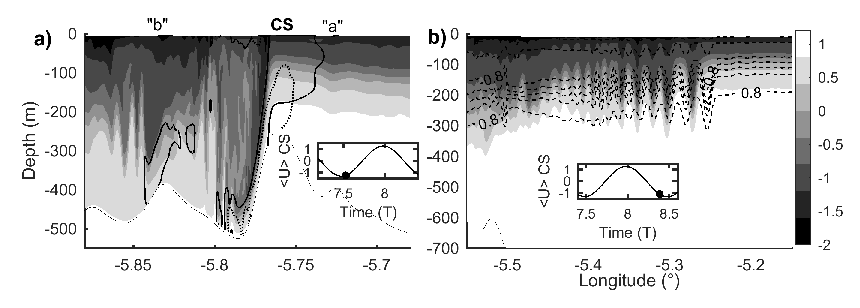
\includegraphics[width=1\textwidth]{./GBR2D/figure10.eps}
  \caption{Comparison of experiments \textbf{SimS} and \textbf{SimRef} showing the effect of tidal amplitude on the generation of solitary waves. a) Relative density ($kg/m^3$) in \textbf{SimS} during a hydraulic jump ($t = 7.5\ T$) at Camarinal Sill. Regions where $F\ >\ 1$ are indicated for both \textbf{SimS} (bold lines) and \textbf{SimRef} (dashed lines). New features appear with stronger tides: a mode-1 disturbance "a" trapped upstream of the CS; an additional supercritical area ($F\ >\ 1$) noted "b" in the bottom layer of a secondary relief. b) Relative density in \textbf{SimS} (greyscale) and \textbf{SimRef} (dashed lines) at $t = 8.5\ T$, showing the tidal amplitude effect on eastward propagating solitary waves generated at CS.}
  \label{fig_cv_spring}
\end{figure}


%------------------------------------------------------------------
\subsubsection{Nonhydrostatic Balance and Numerical Factors}
\label{TestNum}
%------------------------------------------------------------------
The consequences of several numerical choices are now investigated by running five additional simulations whose differences with \textbf{SimRef} are laid out in Table \ref{tab_sensnum}. In particular, the sensitivity to both vertical and horizontal resolution is targeted. A hydrostatic kernel and a WENO5-Z advection scheme for momentum \citet{Borges2008} are also tested and compared with \textbf{SimRef}. We focus on the impact of these modifications on two types of small-scale processes studied in the previous sections: the primary (KH) instability generation in the hydraulic jump at the CS, and the eastward propagating solitary waves generated at the same place. 

\begin{table}[!h]
\caption{Parameters of numerical sensitivity experiments. If not explicitly indicated, $t_s$ and $t_f$ are the same as in Table \ref{tabsimref}.}
 \centering
  \begin{tabular}{|c|l|}
 \hline
  \textbf{SimH}& Hydrostatic equations ($t_s=0.5s$ ~ $t_f=0.25s$)\\
  \hline
  \textbf{SimW}& WENO5-Z momentum advection scheme\\
  \hline
  \textbf{SimV}& 80 $\sigma$-levels\\
  \hline
  \textbf{SimL}& 220-m horizontal resolution ($t_s=4s$ ~ $t_f=0.5s$)\\
  \hline
  \textbf{SimLH}& 220-m horizontal resolution with hydrostatic equations ($t_s=2s$ ~ $t_f=1s$)\\
  \hline
 \end{tabular}
	\label{tab_sensnum}
\end{table}

%-------------------------------------------------
\paragraph{Hydraulic Jump and Instabilities}
%-------------------------------------------------

\begin{figure}[!h]
\centering
  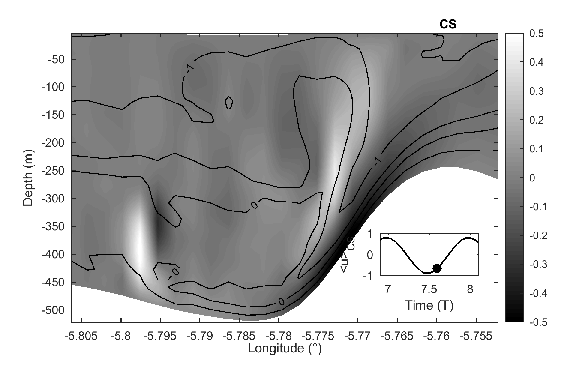
\includegraphics[width=0.7\textwidth]{./GBR2D/figure11.eps}
  \caption {Vertical velocity (greyscale ; $m/s$ ) and isopycnals (black lines ; density anomaly between -1.5 kg m$^{-3}$ and 0.5 kg m$^{-3}$ with an interval of 0.5 kg m$^{-3}$ ) in \textbf{SimLH}.}
	\label{fig_sensnum1}
\end{figure}

Hydraulic controls (Section \ref{tide_hyd}) occur in all simulations, as revealed by systematic estimations of the Froude numbers. Low Richardson numbers ($<0.25$) are also diagnosed for all simulations over at least part of the CS western slope during flood. However, the features that have been identified as KH instabilities in Section \ref{sinsta} do not appear in all simulations. They are absent in the simulations performed in the hydrostatic framework and/or with low horizontal resolution (\textbf{SimL}, \textbf{SimLH} and \textbf{SimH}). Weak horizontal vorticity tilting under the hydrostatic assumption prevents such instabilities to develop. Instead, a smooth, large recirculation  appears west of the CS (Figure \ref{fig_sensnum1} for \textbf{SimLH}).

In the remaining sensitivity experiments (\textbf{SimV} and \textbf{SimW}), KH instabilities are generated at the edge of the hydraulic jump and their dynamics is overall similar to the one described in Section \ref{sinsta} for \textbf{SimRef}: pairing of KH billows can occur whereas anti-clockwise vortices induce oscillations of the interface. 
Fine resolution (a few tens of meters in the present region) and non-hydrostatic equations are both required to explicitly simulate the turbulent cascade onset with KH instabilities between Mediterranean and Atlantic flows. 

Interestingly enough, a comparison of Figures \ref{RH_CS} (nonhydrostatic configuration) and \ref{fig_sensnum1} (hydrostatic configuration) shows that the fine-scale solution is largely filtered out by the hydrostatic assumption. Without dedicated observations in the area, it remains difficult to conclude that \textbf{SimRef} is more realistic, although low Richardson numbers in this region lead us to expect KH instability.

\paragraph{Large Internal Waves}
\begin{figure}[!h]
  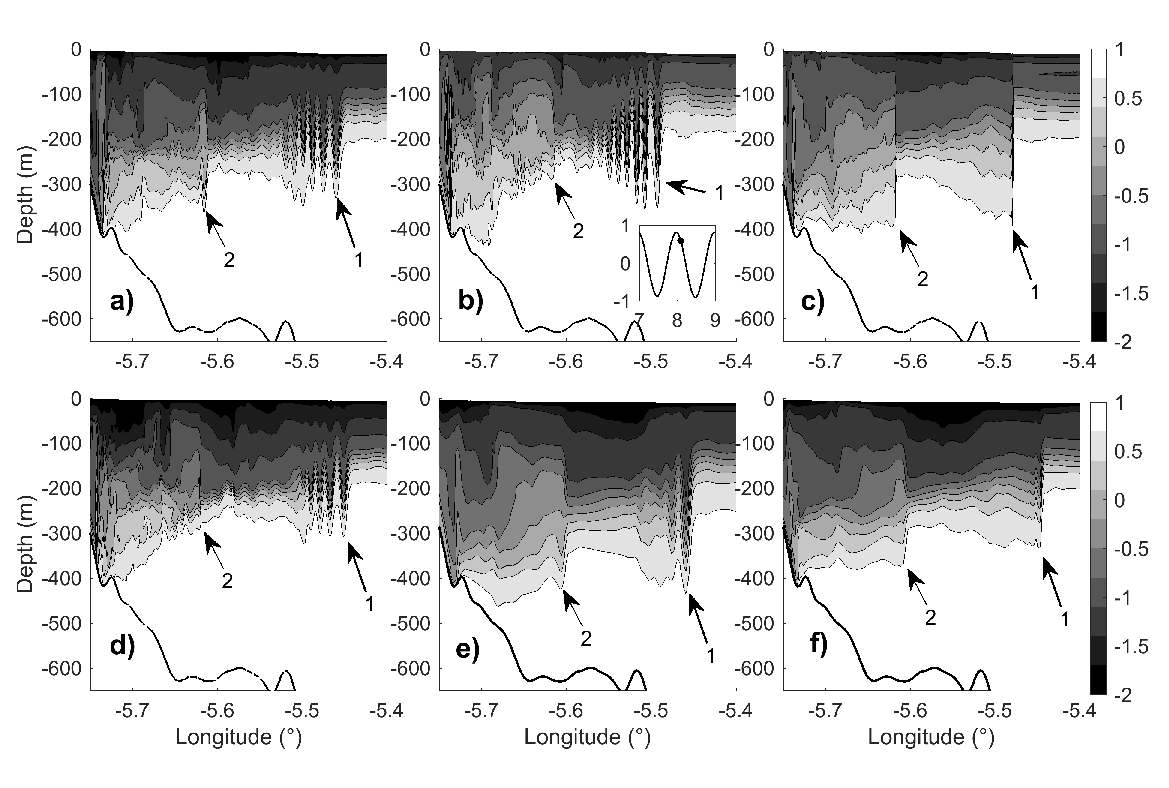
\includegraphics[width=\textwidth]{./GBR2D/figure12.eps}
  \caption{Internal wave propagation from density field at $t = 8.1 T$ in (a) \textbf{SimRef}; (b) \textbf{SimW}; (c) \textbf{SimH}; (d) \textbf{SimV}; (e) \textbf{SimL}; and (f) \textbf{SimLH}. Large amplitude mode-1 waves (soliton or bore) are denoted as "1" and mode 2 as "2".}
  \label{fig_trains_num}
\end{figure}

As described in Section \ref{sisw}, mode-1 and mode-2 large amplitude internal waves are generated in the CS vicinity and propagate eastward during each ebb in all nonhydrostatic simulations. Figure \ref{fig_trains_num} presents the density fields in the region of the TN at $t\ =\ 8.1\ T$. A wave train with a minimum of two solitons can only be identified in the nonhydrostatic experiments. In the hydrostatic cases \textbf{SimH} and \textbf{SimLH}, the lack of nonhydrostatic dispersion produces internal waves propagating as internal bores. In the nonhydrostatic cases, these internal waves can propagate as trains of solitons with varying numbers of solitons (and celerity) : 6 in \textbf{SimRef}, 8 in \textbf{SimW}, 4 in \textbf{SimV}, and 2 in \textbf{SimL}. 

This illustrates a second aspect of the effect of hydrostatic assumptions, besides the inhibition of turbulent primary instabilities (KH instabilities in the region of the hydraulic jump). As already noted by previous authors \citep{Sannino2004}, the dispersion needed to balance nonlinear steepening in large-amplitude solitary waves is missing in hydrostatic simulations such as \textbf{SimH} and \textbf{SimLH} (Figure \ref{fig_trains_num}).

%---------------------------------------------------
\paragraph{Evolution of Stratification}
%---------------------------------------------------

\begin{figure}[!h]
\centering
  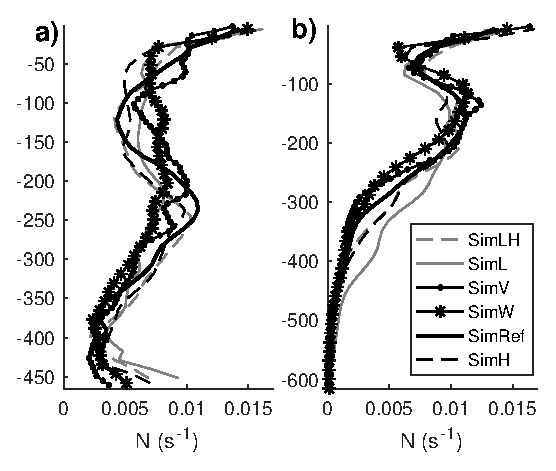
\includegraphics[width=0.7\textwidth]{./GBR2D/figure13.eps}
  \caption {a) $N$ frequency computed at 5.8$^\circ$W longitude and time-averaged between 8.2 T and 8.7 T (during flood tide and presence of hydraulic jump). b) Same as (a) but at 5.55$^\circ$W longitude.}
	\label{fig_sensnum2}
\end{figure}

The previous results lead us to anticipate large differences in the way density stratification evolves in \textbf{SimRef}, \textbf{SimW}, \textbf{SimV}, \textbf{SimH}, \textbf{SimL}, or \textbf{SimLH}. To go further, Figure \ref{fig_sensnum2} shows for each configuration the profiles of Brunt-V\"ais\"al\"a frequency ($N$ defined in eq.\ref{eqN}) at 5.8$^\circ$W (a) and at 5.55$^\circ$W (b). Profiles are time-averaged over one flood. 

At 5.8$^\circ$W, stratification is similar in \textbf{SimH} and \textbf{SimLH} with an interface region (defined as the region where $N$ is maximal, here $N$ = 8.10$^{-3}$ s$^{-1}$) located at a depth of 250 m (Figure \ref{fig_sensnum2}.a). The nonhydrostatic simulations \textbf{SimRef} and \textbf{SimL} present an interface region at a similar depth but the vertical gradients are larger in \textbf{SimRef} and smaller in \textbf{SimL}.
\textbf{SimV} shows larger vertical gradients of density ($N$ = 1.1 10$^{-2}$ s$^{-1}$) and a shallower interface at a depth of 150 m. \textbf{SimW} is weakly stratified over most of the water column with no clear interface between the two water masses. This result may seem surprising because the WENO5 scheme is of fifth-order accuracy with more selective quasi-monotonic corrections near shocks than the TVD scheme, and is thus expected to produce less smoothing. This apparent contradiction can be explained by the generation of more intense primary shear instabilities (i.e. with higher values of associated vertical velocity and vertical velocity gradients), which has the effect of diffusing density gradients.

In Figure \ref{fig_sensnum2}.b, averaged $N$ profiles over one flood  are shown at 5.55$^\circ$W longitude in a region subjected to intense internal wave activity. \textbf{SimH}, \textbf{SimLH} and \textbf{SimL} exhibit similar profiles with $N$ slowly decreasing below the interface at 160 m. \textbf{SimRef} has a similar interface at 160 m but with higher $N$ value, although weaker stratification appear at the top of the lower layer. \textbf{SimV} and \textbf{SimW} both have shallower interfaces at 130 m, with $N$ reaching the highest values in \textbf{SimV} ($N$ = 1.25 10$^{-2}$ s$^{-1}$), as the enhanced vertical resolution allows the representation of stronger gradients.

Clear conclusions cannot yet be drawn concerning mixing. KH instabilities are expected in the region of the hydraulic jump and downstream. They lead to more stirring and consequently open up new opportunities to improve modelling of the route to mixing. Further investigation and diagnostics are now required to better understand the energy cascades. In particular, the present comparison between WENO5 and TVD advection schemes (and their implicit dissipation) indicates that numerical choices may unfortunately still have large consequences. Therefore, the role of physical and numerical closure must be considered comprehensively \citep{Marchesiello2011, Soufflet2016}.

%%%%%%%%%%%%%%%%%%%%%%%%%%%%%%%%%%%%%%%%%%%%%%%%%%%%%%%%%%%%%%%%%%%%%%%%%%%%%
\subsection{Discussion and Conclusion}
%%%%%%%%%%%%%%%%%%%%%%%%%%%%%%%%%%%%%%%%%%%%%%%%%%%%%%%%%%%%%%%%%%%%%%%%%%%%%

The present study focuses on small-scale dynamics in the Strait of Gibraltar and on the capacity of a new split-explicit, free-surface, nonhydrostatic regional oceanic model (CROCO) to represent such dynamics. Both objectives were pursued in parallel and several seminal results are obtained.

The study confirms that the generation of large-amplitude mode-1 and mode-2 internal waves in the Strait of Gibraltar as well as the onset of stratified turbulence and its energy cascade can be simulated with a computationally-efficient 2D vertical section. The characteristics of the simulated internal waves compare qualitatively well with published observations and previous numerical studies. Internal tides dynamics and shear instability in the hydraulic jump area are then analysed in more details, revealing characteristics and mechanisms.
 
The results of the study rely on a new type of nonhydrostatic, non-Boussinesq, free-surface kernel \citep{Auclair2018} implemented in the CROCO model. The resulting compressible oceanic model is presented in a realistic nonhydrostatic configuration for the first time. Sensitivity tests confirm that a nonhydrostatic (here non-Boussinesq) kernel is required (i) to simulate ISW trains and (ii) to explicitly simulate the onset of stratified turbulence energy cascade, provided that resolution is increased from about 200 m to 50 m. We conclude that resolutions finer than a few hundred meters are required in addition to a refinement of dynamical equations (relaxation of hydrostatic assumption) in order to solve the dominant dynamical processes in a key region of the Mediterranean.

Detailed characteristics of the vertical 2D configuration are also given with particular attention to the bathymetry and to the representation of the Coriolis force (implicit representation of funnelling effect in the strait). The proposed approach offers a computationally affordable way to make preliminary investigations of internal-wave dynamics in regions where these waves are important. However, the vertical 2D configuration is limited by the simplified representation of bathymetry and associated biases in the velocity shear between in-flowing Atlantic Waters and out-flowing Mediterranean waters. The inclusion of restratification processes (surface and boundary forcing) would allow the model to remain accurate for a greater number of tidal cycles --- the present configuration is considered accurate within three days after the spin-up period, before mixing starts to homogenise the water masses. Several remaining processes could not be considered: the transverse propagation of ISWs in the Strait of Gibraltar \citep{SG2011, Vlasenko2009} and in the Alboran Sea; the hydraulic control at the TN \citep{FA1988, Sannino2009b}; the boiling-water over the CS \citep{Bruno2002} or reflections on the strait's coasts. 

Only the ``onset'' of turbulence cascade could be simulated showing complex dynamics occurring in the area of the hydraulic jump at CS, with some small scale features identified as primary Kelvin-Helmholtz instabilities. Although this 2D study highlights how interesting this area can be, there is no doubt that simulation of secondary KH instabilities and subsequent energy cascade as well as the long term impact of these small scale processes on Mediterranean and North Atlantic circulation will require a fully 3D LES approach as well as dedicated field campaigns that explore these fine-scale processes.


%%%%%%%%%%%%%%%%%%%%%%%%%%%%%%%%%%%%%%%%%%%%%%%%%%%%%%%%%%%%%%%%%%%%%%%%%%%%%
%\appendix
%%%%%%%%%%%%%%%%%%%%%%%%%%%%%%%%%%%%%%%%%%%%%%%%%%%%%%%%%%%%%%%%%%%%%%%%%%%%%
\section{(annexe)Evaluation of the First Internal Rossby Radius}
\label{app_Rossby}
%%%%%%%%%%%%%%%%%%%%%%%%%%%%%%%%%%%%%%%%%%%%%%%%%%%%%%%%%%%%%%%%%%%%%%%%%%%%%

The first internal Rossby radius is defined as :
\begin{equation}
\label{eqRosby}
R = \frac{\sqrt{g'h}}{f}
\end{equation} 
 At the Gibraltar Strait's latitude, the Coriolis parameter is $f=8.5 \times 10^{-5}\ s^{-1}$.
The numerator $c^{*}={\sqrt{g'h}}$ is the phase speed of the linear interfacial waves, into which the reduced gravity is:
\begin{equation}
g'= g \frac{\rho_M(S_M) - \rho_A(S_A)}{\rho_0}
\end{equation}
where $\rho_M(S_M) - \rho_A(S_A) \approx 2\ kg/m^{3}$. If the reference density is set to $\rho_0=1033.7\ kg/m^{3}$ and the gravity acceleration by $g=9.81\ m^2/s$, $g'=0.02\ m/s^{-2}$ which is in agreement with in situ data (cf \citet{Bryden94}). $h$ is a characteristic height given by:
\begin{equation}
h=\frac{h_1 h_2}{h_1+h_2}
\end{equation}
where $h_1$ and $h_2$ are respectively the upper and lower layer thicknesses. Picking up the data values from \citet{FA1988} (Table \ref{tabdepth}, first line), we obtain a range of $h = 50 - 100\ m$, which combined with the previous values for $g'$ and $f$ leads to $R$ ranging in 11.5 km (east of Camarinal Sill) to 16 km (west of Camarinal Sill). 

$\sqrt{g'h}$ can be replaced by the mode-1 internal waves speed($c_1$), which is estimated in the present study (\ref{app_Froude}) for the 3T-averaged stratification (\textbf{SimRef}) presented in Figure \ref{fig_fn_ref}. $c_1$ ranges between 0.8 m/s (at Camarinal Sill) and 1.8 m/s (in the eastern part of the strait), giving an estimated range of Rossby Radius ${c_1}/{f}$ between 9.5 and 21 km for the simulated section.


%%%%%%%%%%%%%%%%%%%%%%%%%%%%%%%%%%%%%%%%%%%%%%%%%%%%%%%%%%%%%%%%%%%%%%%%%%%%%
\section{(annexe)Computation of a Froude Number}
\label{app_Froude}
%%%%%%%%%%%%%%%%%%%%%%%%%%%%%%%%%%%%%%%%%%%%%%%%%%%%%%%%%%%%%%%%%%%%%%%%%%%%%
A single value of mode-n linear internal wave phase speed ($c_n$) can be computed for a flat-bottom and a linear stratification. This velocity can then be compared at each depth with the magnitude of local horizontal currents ($u$) to estimate when and where internal waves can propagate against currents. A diagnostic tool is the ratio of velocities, i.e. a Froude number $(F_n)$ defined as $F_n= u /c_n$. $c_n=\omega / k_n $ where $\omega$ is the wave frequency, here the M2-tidal frequency, and
%\begin{equation}
%\label{eqK}
%k_n=\pm \frac{n \pi}{H} \left( \frac{\omega^2 - f^2}{N^2 - \omega^2} \right) ^{1/2} 
%\end{equation}
$k_n$ are eigenvalues obtained by solving numerically the Sturm-Liouville problem associated with the linear propagation equation \citep{Gill1982}:
\begin{equation}
 W_n'' + k^2 \frac{N^2 - \omega^2}{\omega ^2 - f^2}W_n = 0
\end{equation}
with bottom and surface boundary conditions $W_n(0) = 0$ and $W_n(-H) = 0$. $W_n$ gives the structures of vertical modes. For each point on the x-axis, the profile N(z) is computed with Eq.\ref{eqN} from the 3T-averaged stratification in \textbf{SimRef} (shown in Figure \ref{fig_fn_ref}).

\begin{figure}[!h]
\centering
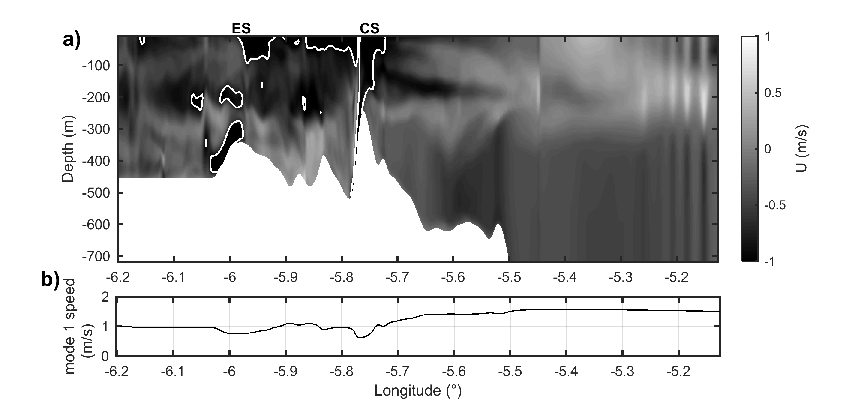
\includegraphics[width=1\linewidth]{./GBR2D/figure14.eps}
\caption{a) Field of longitudinal velocity ($u (x,z)$) at $t = 8.5\ T$ with contours of mode-1 supercritical region (F$>$1) calculated from a 3T-averaged stratification. b) Computed speed of mode-1 linear internal waves ($c_1 (x)$) from a 3T-averaged stratification in configuration \textbf{SimRef}.}
\label{fig_annexeF}
\end{figure}

 The value of the first mode phase speed $c_1(x)$  is indicated in the lower panel of Figure \ref{fig_annexeF} and compared to the longitudinal velocity $u(x,z)$ at $t = 8.5\ T$ plotted in the upper panel. The areas where $u(x,z) > c_1 (x)$ (equivalent to Froude number $F_1$ larger than 1) are presented in the upper panel as well. The flow inside those contours is called supercritical.
 
 %%%%%%%%%%%%%%%%%%%%%%%%%%%%%%%%%%%%%%%%%%%%%%%%%%%%%%%%%%%%%%%%%
 \section{(annexe)Computation of Okubo-Weiss Parameter}
 \label{annexeOW}
 %%%%%%%%%%%%%%%%%%%%%%%%%%%%%%%%%%%%%%%%%%%%%%%%%%%%%%%%%%%%%%%%%
The Okubo-Weiss parameter (OW) is defined as
\begin{equation}
OW=s_n^2+s_s^2-\Omega^2
\label{eqOW}
\end{equation}
With $s_n$ the normal strain component, $s_s$ the shear strain component and $\Omega$ the vorticity. Usually, it is used in a xy-plane (e.g., for tracking eddies in \citet{Chelton2007}), but it is computed here in the zx-plane with the strains and vorticity expressed as :
\begin{equation}
s_n = \frac{\partial w}{\partial z} - \frac{\partial u}{\partial x} \quad , \quad
s_s = \frac{\partial u}{\partial z} + \frac{\partial w}{\partial x} \quad , \quad
\omega = \frac{\partial u}{\partial z} - \frac{\partial w}{\partial x}
\end{equation}
Negative values of OW indicate a greater role of rotation over deformation, and thus the presence of coherent vortices.

 %%%%%%%%%%%%%%%%%%%%%%%%%%%%%%%%%%%%%%%%%%%%%%%%%%%%%%%%%%%%%%%%%
\section{(annexe)Comparison with Korteweg-de Vries (KdV) Model}
\label{KdVpart}
%%%%%%%%%%%%%%%%%%%%%%%%%%%%%%%%%%%%%%%%%%%%%%%%%%%%%%%%%%%%%%%%%%%%%%
\begin{figure}[!h]
\centering
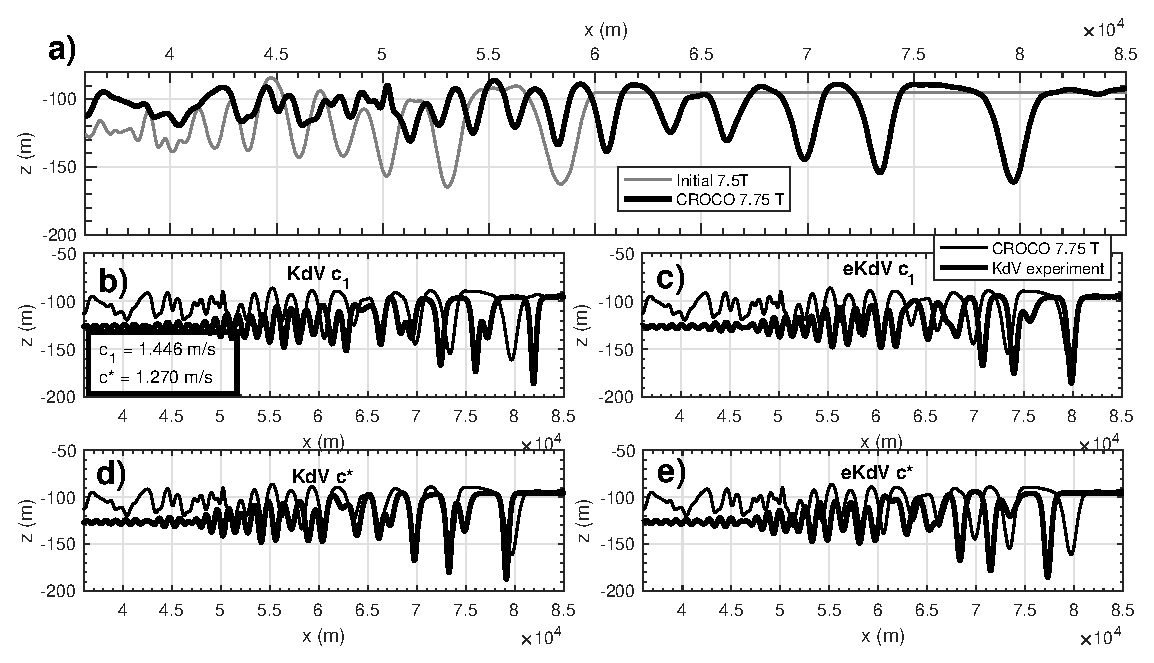
\includegraphics[width=1\linewidth]{./GBR2D/figure15.eps}
\caption{ a) Isopycnal $\rho$'\ =\ -0.2\ kg/m$^3$ simulated by CROCO in \textbf{SimRef+} at $t\ =\ 7.5\ T$ (grey line; the interface depth is left constant downstream of the wave) and at $t\ =\ 7.75\ T$ (black line). b-e) Evolution of the interface simulated by KdV or eKdV (bold) and \textbf{SimRef+} (solid line) at $t\ =\ 7.75\ T$. Two propagation speeds are used: c$^*$ (d,e) and c$_1$ (b,c) (see text for details).}
\label{fig_kdv}
\end{figure}

Following many studies \citep{SG2008, Sannino2009b, Vlasenko2009}, the large amplitude internal waves of Section \ref{sisw} are termed ''ISWs'' for Internal Solitary Waves. To confirm that the internal waves observed in this section are ISWs, they are now compared with solutions of the Korteweg-de Vries equation which is recalled below. The solutions of this equation satisfy a balance between nonhydrostatic dispersion and nonlinear advection. Nonlinear advection steepens the wave front, whereas nonhydrostatic dispersion reduces steepening by transferring energy from large to small scales, resulting in a relatively stable entity called a ''solitary'' wave, or soliton.

The Korteweg-de Vries (KdV) equation describes the evolution of an infinitely thin interface in a two-layer system with constant bottom topography:
\begin{equation}
\frac{\partial \zeta}{\partial t} 
+c^* \frac{\partial \zeta}{\partial x}
\underbrace{+ \frac{3}{2} \frac{h_1-h_2}{h_1h_2} c^* \zeta \frac{\partial \zeta}{\partial x} }_{A}
\underbrace{+ \frac{1}{6} h_1h_2c^* \frac{\partial ^3 \zeta}{\partial x^3} }_{B}
\underbrace{ - \frac{3}{8}\zeta^2c^*\frac{h_1^2+6h_1h_2+h_2^2}{8(h_1h_2)^2} }_{C}
=0
\label{eq_kdv}
\end{equation}
where $c^*$ is the interfacial speed of small-amplitude internal waves: $c^*=\sqrt{g' h}\ = \ R.f$ and $\zeta$ is the vertical displacement of the interface. $g'$ and $h$ have already been defined in \ref{app_Rossby}.
%
The first two terms on the left-hand-side of (\ref{eq_kdv}) are those involved in the classical propagation equation for a small-amplitude, linear, interfacial wave travelling in the x-direction at speed $c^*$. The third term (bracket A) is a first-order approximation (with respect to amplitude) of nonlinear advection. Term (B) is a dispersive term.
%
The fifth term (C) is a higher-order non-linear term associated with a second order development for advection. The complete equation (\ref{eq_kdv}) will be referred to as "extended KdV" (or "eKdV"), whereas the same equation without term (C) will simply be referred to as "KdV" \citep{Dossmann2012}.

The simulated large amplitude waves presented in this study are compared with the solutions of the KdV or eKdV equation to gain insight into their dynamics. For optimal comparison, a new simulation, called \textbf{SimRef+} was carried out. Its characteristics are similar to \textbf{SimRef} (Table \ref{tabsimref}), except that (i) the eastern boundary is shifted 42-km to the east into the Mediterranean sea and (ii) the tidal forcing is stopped after only 7.25 periods. The first eastward-propagating train of mode-1 waves generated by the tide at the CS is compared with the propagation given by numerical integration of the KdV and eKdV equations (eq. \ref{eq_kdv}).

The vertical displacement of isopycnal $\rho'\ =\ -0.5\ kg/m^3$ is extracted\footnote{Due to the extension of the domain to the east, a new value of $\rho_0$ is computed : $\rho_0\ =\ 1033.9 \ kg/m^3$ to optimize computations.} at $t_0\ =\ 7.5\ T$ when the mode-1 ISW train propagates over a region of constant depth ($H\ =\ 890\ m$) east of TN (Figure \ref{fig_kdv}), so as to get closer to the KdV framework. The position of the chosen isopycnal surface at this time is shown in Figure \ref{fig_kdv}.a. At that time, the distance between the first and second solitons of the train is 5 km; the first soliton has an amplitude of 75 m and the train includes 7 solitons. This isopycnal is chosen as initial state for the KdV or eKdV model. 
%
The KdV and eKdV equations are integrated either with the interfacial wave speed ($c^* \approx 1.27\ m/s$) or with mode-1 velocity ($c_1 = 1.45\ m/s$; see \ref{app_Froude} for details on $c_1$ evaluation).

Figures \ref{fig_kdv}.b-e compare the interface depth obtained at $t\ =\ t_0\ +\ 0.25\ T$ in the KdV and eKdV models with the position of the $-0.5\ kg/m^3$ isopycnal in \textbf{SimRef+}. In the latter, the distance between the first two solitons has grown since $t =\ t_0$ and reaches 7 km with an amplitude of 70 m for the first trough. The train is now made of 11 solitons: the first three have decreasing amplitudes, then two smaller solitons of comparable amplitude (40 m) and one soliton of greater amplitude, followed by solitons with decreasing amplitude again. 

In the KdV solution obtained with propagation speed c$^*$ the first solitary wave is slightly slower but its amplitude is markedly larger (Figure \ref{fig_kdv}.d). The remaining solitons of the train are well located, but a secondary trough is generated between the first two solitons whereas it is absent in \textbf{SimRef+}.

Using the larger mode-1 speed $c_1$ instead of $c^*$ (Figure \ref{fig_kdv}.b), the train of solitons in KdV is too fast. When the eKdV equation is used with speed $c^*$ (e), the solitons are too slow, whereas this same extended equation with $c_1$ (c) leads to a correct displacement of the solitons. 
Overall, the temporal evolution of solitary waves in \textbf{SimRef+} is consistent with the solutions of the KdV or eKdV equation (\ref{eq_kdv}). However, the KdV or eKdV framework remains an inviscid simplification. Note that closer evolution of soliton amplitudes between KdV or eKdV and \textbf{SimRef+} solutions can be obtained by simply adding a diffusive term in KdV or eKdV equation. This also slows down propagation in KdV, and to a lesser extent in eKdV (not shown).

The KdV or eKdV model also involves adjustable parameters, such as the linear wave speed, which ranges between the interfacial speed $c^*$ and the mode-1 speed $c_1$, each being one particular approximation of the wave's behaviour. 

That being said, the wave trains in \textbf{SimRef+} are appropriately modeled as KdV or eKdV ISWs, which confirms (i) the propagation of interfacial troughs as trains of solitons and (ii) CROCO's ability to simulate the subtle balance between nonhydrostatic effects (responsible for dispersion) and nonlinear advection. 
 
%%%%%%%%%%%%%%%%%%%%%%%%%%%%%%%%%%%%%%%%%%%%%%%%%%%%

\paragraph{Acknowledgments} This work was partly funded by the DGA "Etude Amont" Protevs driven by the Shom. It was granted access to the HPC ressources of CALMIP supercomputing center under the allocation P18017. We also gratefully thank the computer team of the \textit{Laboratoire d'Aérologie} for its support. Margaux Hilt's PhD thesis was funded by a MESRI scholarship. 


%\bibliography{biblio_gib_doi}

%\end{document}



%%%%%%%%%%%%%%%%%%%%%%%%%%%%%%%%%%%%%%%%%%%%%%%%%%%%%%%%%%
%%%%%%%%%%%%%%%%%%%%%%%%%%%%%%%%%%%%%%%%%%%%%%%%%%%%%%%%%%
\chapter{Simulation des grandes structures turbulentes (LES, 3D) dans le détroit de Gibraltar}
%\chapter{Fines scales \& Large Eddy Simulation in Gibraltar Strait}
%%%%%%%%%%%%%%%%%%%%%%%%%%%%%%%%%%%%%%%%%%%%%%%%%%%%%%%%%%
%%%%%%%%%%%%%%%%%%%%%%%%%%%%%%%%%%%%%%%%%%%%%%%%%%%%%%%%%%
\label{chapGBR3D}
 
%%\selectlanguage{english}
\hypersetup{pdfborder=0 0 0}
%\vspace{10\baselineskip}


%\selectlanguage{french}


\section{Resume français}




%-------------------------------------------------------------------------------------
\section{Papier 3D}
\subsection{Introduction}

The Atlantic - Mediterranean exchange occurring in the Strait of Gibraltar has been explained summarily in previous part (2D). It consists in Med waters exiting the Strait at depth as what has been dubbed the 'Mediterranean outflow' while Atl waters enter the Mediterranean basin at the surface.

Those Atlantic waters entering at the Strait are the principal contribution to the Mediterranean inflowing water budget, with the average transport of Atl waters at Gib being of the order of 1Sv. The net exchange itself is of the order of 0.1Sv as a positive entry that offsets the otherwise net evaporation occurring on the integrated surface of the Mediterranean basin \citep{bryden_1994}.
Since the Med basin is otherwise a closed basin, the Mediterranean waters exiting the Strait of Gibraltar are the result of the transformations into intermediate and deep water masses of the Atl waters that circulated in the Mediterranean.
More details are provided in this section on the characteristics of the Strait, the exchange and its variability and the processes that take place during it.






\subsubsection{Circulation in neighbouring areas (Cadix and Alboran)}

(de Pascual-Collar ; NAjanro 2012 ; Sanchez Garrido 2013 ;Lorente 2019 ; garcia lafuente 2017)


\textit{Atlantic side}

The surface waters that end up entering the Strait are NACW and SAW\citep{millot_2014,naranjo_2015}. They are carried by the Portugal and Azores Current into Gib as part of the eastern branch of the north atlantic subtropical gyre \citep{barton_2001}

Below this surface circulation, can find in the Northern Atlantic the med outflow/the mediterranean watermass that was transported out of the Strait by the MEditerreanaen outflow. It first flows in the Gulf of Cadix, rotating to north due to geostrophy and flowing along the bathymetry of the continental slope\citep{price_1993,gasser_2017} and west of the Gulf of Cadiz stabilizes to its neutral buoyancy level at 1000m depth as the Mediteranean water mass\citep{price_1993}. Meddies, salty lenses of water with negative (?) vorticity able to 'survive' for years that are encountered in the open ocean, are generated along the canyons and caps encountered by the Mediterranean outflow in the Gulf of Cadiz \citep{bashmachnikov_2015}. The Mediterranean outflow itself participates in the global circulation/north atlantic overturning circulation(?) by salinification of the overall north atlantic basin with the spreading of the mediterranean water mass in the open ocean and decaying of meddies, but also with a part of the outflow directly joining circulation at the pole \citep{price_1993,jia_2007}.


\textit{Mediterranean side}


Surface waters exiting the Strait at the east enter the Alboran Sea as the Atlantic Jet (AJ). The circulation of the Alboran Sea is variable, with the most common state having two anticyclonic gyre (WestarnAlboranGyre ans EasternAlboranGyre), but not uncommon that only one of the two is present \citep{millot_2005}. The WAG is coupled to the Atlantic jet, that usually constitutes its northern branch, however variability of the AJ due to meteorological and tidal forcing can destabilize this system \citep{sanchez-garrido_2013,lorente_2019}.

At depth, several mediterranean water masses enter the strait. In the Alboran Sea, identified are LIW (for Leventine Intermediate Water) and WMDW(West MEditerranean Deep Water), with other water masses of the western med bassin like TDW (Thryenian Deep Water) also being detected (maybe)(Millot). There is a south/north repatition of those watermasses, with TDW, LIW and other intermediate waters more abundant in northern part of Alboran sea, and WMDW flowing more in south part \citep{millot_2014}. As the depth from teh Alboran to the Strait decreases, it is more difficult for the deeper WMDW to enter the strait, and the flow can be regulated by mechanisms such as the strength of the WAG or the overall production of WMDW linked to winter convection (Najanro 2012).


\textit{Gen}

Whether look at inflowing (in reference to the med basin) Atl waters or outflowing (ditto) Med waters, they incorporate signature of respectively the med waters (Macias 2006) and atl waters (Millot 2006,GarciaLafuente2011). This is due to mixing occurring in the Strait, driven by small scale processes of varying strength. 


%%%%%%%%%%%%%%%%%%%%%%%%%%%%%%%%%%%%%%%%%%%%%%%%%%%%%%%%%%%%%%%%%%%%%%%%%%%%
\subsubsection{Morphologie et marée barotrope et masses d'eaux (et ajouter atm???)}
%%%%%%%%%%%%%%%%%%%%%%%%%%%%%%%%%%%%%%%%%%%%%%%%%%%%%%%%%%%%%%%%%%%%%%%%%%%%%


The Strait is inclined of 15$^\text{o}$ from the east direction. Away from continental plateau, Camarinal Sill is the shallowest point with depth averaging at 300m. Relative to Camarinal Sill, Strait is narrower but deeper on the east side. On the west side, shallower, with two troughs on each side of a submarine mount called Majuan Bank. The northern trough is shallower than the southern one, which also includes another sill, called Espartel Sill. Those two troughs are the two pathways the Med outflow take to join the Gulf of Cadix, with most of the flow taking the southern deeper path (18 \% au nord selon Soto-Navarro 2014)


The barotropic M2 semi-durnal tide from the North Atlantic is the foremost varying signal for the currents in the Strait, propagating from south to north with amplitude decreasing from west to east\citep{candela_1990}. During Flood (ebb) tide, barotropic currents ate westward(eastward). The Currents associated with the barotropic tide are same amplitude as the mean circulation, can reverse the flow of med and/or atl waters for certain sections(Sanchez Roman 2012), and have a pronounced neap-spring tide cycle.

Wind is funnelled through the strait and is either westward or eastward/principally zonal with speed can reach 25m/s(Candela 1989). Wind stress affects only the first tens of meters of circulation in the Strait (Candela 1989), which can be sufficient to affect the Atlantic Jet, either accelerating(and making it exit the Strait at various angle) or decelerating it(can even stop it)(Lorente2019). Otherwise, the integrated effect of atmospheric pressure over the Mediterranean basin influence the net flow through the Strait(Garcia Lafuente 2002).





%%%%%%%%%%%%%%%%%%%%%%%%%%%%%%%%
\subsubsection{Baroclinic Exchange and small scale processes}


The circulation of eastward Atlantic waters at the surface and westward Mediterranean waters at depth sets up a baroclinic exchange in the Strait of Gibraltar. Due to amplitude of the barotropic currents, it is intermittent with regard to the M2 tide. One can thus see the exchange as a Reynolds(?) decomposition of an average with tidal contribution as eddy-fluxes that impacts secondary characteristics of the exchange (Naranjo 2014, etc..), and which have a more important amplitude at CS (Vargas2006).  

The exchange varies with other greater timescales than the semi-diurnal tide, with the lower frenquencies (seasonal,interannual) usually linked to atmospheric forcing over the Mediterranean (SanchezRoman2012?). But the tidal eddy-fluxes have their own variability linked to the spring-tide cycle and monthly tide, with for example a greater depth and stronger shear during neap tides, but more intense mixing in spring tide (Naranjo 2014, Vargas 2006).

Behind those characteristics varying at the tidal time-scale are small scale processes occurring in the Strait of Gibraltar.



Firstly, due to the limited horizontal and vertical extent of the Strait that channels the superposed average exchange flow and barotropic tidal currents, the flow in the Strait can become supercritical in regard to internal gravity wave propagation. East (west) of the Camarinal Sill the flow in atl (resp. med) layer will become supercritical, although the detail of how regular/their disposition and geometrical extent depends on the framework one uses. (exemples: Farmi et Armer 1988,Sannino 2007,Sanchez Roman 2012,Vargas 2006...)In particular, hydraulic control occurs at Camarinal Sill episodically.

There, development of two hydraulic jump reflecting the geometry of teh sill and can be observed on satellite imagery (brandt1996).The hydraulic jump stays approximately 4 hours at CS during outflows(Vlasenko 2009) and is where intense mixing occurs (Wesson andGregg;Lafuente...2011,MAcias2006(?)), billows from Kelvin-Helmoltz type instability of the flow in the lee of the hydraulic jump and advected westward by med waters(Wesson andGregg). In addition Bruno 2013, the establishment of hydraulic jump brings chlorophyll-rich waters in the center of the Strait.

Then propagate as LAIWs (Large amplitude Internal waves) also called solitary waves (.Farmer and Armi 1988) due to balance between non-linear and non-hydrostatic dispersion. Have been observed at the surface, and at depth (Ziegenbein (1970), Watson and Robinson 1990,Farmer and Armi 1988,SanchezGarrido 2008,etc.). They transport some chlorophyll (Bruno2013) and expect to make remote mixing in Alboran Sea.

ISW are generated at each tide except when westward current are not strong enough for hydraulic criticality at for neap tide (Watson and Robinson 1990, Garcia Lafuente 2000). Refracted as it exits the Strait by interaction with its boundaries, either as a curve or asymmetrically with an angle in the north(Watson and Robinson 1990).

The hydraulic jump and generation process can be achieved in numerical simulation by hydrostatic models but need non-hydrostatic one for propagation (Brandt 1996 ; (Vlasenko 2009)).



%%%%%%%%%%%%%%%%%%%%%%%%%%%%%%%%%%%%%%%%%%%%%%
\subsubsection{Impact, num et Plan}

Those small scale processes are responsible for the mixing of atl and med waters in the Strait, and the characteristics of the water masses involved in the baroclinic exchange at Gibraltar are not conserved(garcia lafuente 2017 : difficult to link characteristics at ES (INGRES, long term mooring to monitor outflow) to processes in the Mediterranean). The enhanced mixing in the Strait then has to be parametrized in coarsely resolved global/regional models the feedback to/in water mass composition that will impact circulation of the MEditerranean and North Atlantic. 


Following Hilt2020, here 3D sigma model,non-hydrostatic and decadal horizontal resolution that at least resolves the greater scales of mixing in the Strait. In particular focus of different tidal forcing case along a neap-spring tide cycle, how the flow characteristics and intensity of mixing processes is affected in simulation by this variability.


The numerical simulation framework constituted of three simulation periods is presented in section \ref{section3Dnum}, with various diagnosis that have been applied to said simulations /experiments then presented (blah) in section \ref{PartDiag3D} . Section \ref{section3DRes} presents results pertaining to the hydrological state of the flow depending on the strength of barotropic tidal currents, the propagation of ISW in the simulations, then areas of generation of primary instabilities, ending with a comparison of turbulence scheme.






\subsection{Numerical Configuration}
\label{section3Dnum}
\subsubsection{Numerical framework}

Simulations are run using CROCO-NBQ as was the case in Hilt 2020 (see a presentation of CROCO-NBQ there ... and in introduction of manuscript???) . Table \ref{tab_NH-HR} summarize some simulation choice. Otherwise, Non-linear equation of state, noslip condition at the bottom,etc...  The turbulent closure scheme used in all simulations except the ones of paragraph ... is Smagorinsky with coef chosen 0.05. For paragraph ... three simulations use Smago with coefs $10{-3}$,$10{-2}$,$10^{-1}$ , and one use GLSk-$\epsilon$.

Bathymetry data from 100m resolved MNT SHOM, smoothed for pressure gradient... is shown in figure \ref{FigBathy3D}. (bathy seuillée?)


Initialisation and open boundary conditions (that incude tdial forcing) are from a simulation of the operational Med and Black Sea ENEA using MitGCM (ENEA, Rome)\footnote{http://www.enea.it/it/seguici/pubblicazioni/pdf-volumi/cresco-report-2016.pdf}, whch serves as parent simulation. The parent simulation as an horizontal resolution in the strait of $\approx$ 700m and vertical z-levels (repartition?), that are interpolated on grid of horizontal resolution 45 m with 40 evenly spaced vertical $\sigma$-levels. As noted in table ..., this is sufficient to be more resolved in the vertical direction than in the horizontal for the whole simulation domain. At Camarinall Sill, vertical resolution varies from $\approx$7.5m at the top to $\approx$12.5m downslope. No atmospheric forcing is embedded in the simulation.

The first 6 hours of simulation are run in CROCO-Hydro at 50m resolution and the last field is used to restart in NBQ mode. Otherwise the balance in MitGCM is to coarse for stability at high resolution.

\begin{table}[!h]
        \centering
        \begin{tabular}{|p{\linewidth/3}|c|c|}
                \hline
                Grid Extension & \multicolumn{2}{c|} {6°4.8'W  5°3.4'W ;}\\
                & \multicolumn{2}{c|} {35°23.8'N  36°27.4'N}\\
                Number of horizontal grid points & \multicolumn{2}{c|} {2049x2621}  \\
                Number of vertical $\sigma$-levels & \multicolumn{2}{c|} {40} \\
                $\Delta x = \Delta y$ & \multicolumn{2}{c|} {45 m}\\
                Depth & Min & Max\\
                & 26 m & 960 m\\
                $\Delta$z & 0.7 m & 24 m\\
                Internal time-step ($\Delta t_s$) & \multicolumn{2}{c|} {1 s}\\
                External time-step ($\Delta t_f$) & \multicolumn{2}{c|} {1/11 s(change 1/14)}\\
                Advection scheme & \multicolumn{2}{c|} {WENO-5} \\
                Viscosity $\nu$ & \multicolumn{2}{c|} {10$^{-6}$ m$^2$/s} \\
                Diffusivity $K_\rho$(aussi Ks et Kt) & \multicolumn{2}{c|} {10$^{-6}$ m$^2$/s}\\
                Pressure/accoustic wave speed$C_s$ & \multicolumn{2}{c|} {400 m/s}\\
                Tidal harmonics (from ENEA) & \multicolumn{2}{c|} { $\text{M}_{\text{2}}$, $\text{S}_{\text{2}}$,$\text{K}_{\text{1}}$, $\text{O}_{\text{1}}$ }\\
                \hline
        \end{tabular}
        \captionof{table}{Simulation parameters}
        \label{tab_NH-HR}
\end{table}


\begin{table}[!h]
        \centering
        \begin{tabular}{|c|c|}
                \hline
                Closure scheme & Simulation name\\
                \hline
                Smago 0.005 & SimIT,SimNT,SimST\\
                Smago 0.001 & SimIT-S001\\
                Smago 0.01 & SimIT-S01\\
                Smago 0.1 & SimIT-S1\\
                GLS K-$\epsilon$ & SimIT-Kep\\
                \hline
        \end{tabular}
        \captionof{table}{Simulation names (ou combiner avec tableau d'avant ???)}
        \label{tab_sim3Dnames}
\end{table}


\subsubsection{Tidal forcing and simulation period}
The tidal forcing is integrated to the boundary forcing by the parent simulation. As indicated in table \ref{tab_NH-HR},  it comprises four tidal harmonics (?)($\text{M}_{\text{2}}$, $\text{S}_{\text{2}}$, $\text{K}_{\text{1}}$, $\text{O}_{\text{1}}$). Due to computational cost constraints, simulations are run for 3 days along 3 different periods of September of year 2017 (close to equinox). The date of the beginning and end of each NBQ simulation is surmised in table \ref{tab_dates_MIV}, and does not include the 6hour hydrostatic spin up period. The comparison of the sea-level anomaly between a grid point near Tarifa (coord -5.6° - 36.01°) in both the parent MitGCM and CROCO simulation and the tidal gauge data (from Puertos del Estado) are shown in figure \ref{fig_maree_tar}. Can see close to the parent simulation except in the neap tide period.

\begin{table}[h]
        %\begin{minipage}{.6\textwidth}
        \centering
        \begin{tabular}{|c|c|c|}
                \hline
                Situation & Simulation name & Dates (UTC)\\
                \hline
                Intermediate Tide & SimIT & 10/09/2017 19h00 - 13/09/17 01h00  \\
                Neap Tide& SimNT & 13/09/2017 16h00 - 15/09/17 17h00 \\
                %\hline
                Spring Tide& SimST & 19/09/2017 22h00 - 21/09/17 23h00  \\
                \hline
        \end{tabular}
        \captionof{table}{Périodes de simulation pour les 3 sitituations VE, MM et ME}
        \label{tab_dates_MIV}
        %\end{minipage}
\end{table}

\begin{figure}[!h]
        \includegraphics[width=0.5\textwidth]{./GBR3D/FigBathyVHR.png}
        \caption{Area and Bathymetry used for the simulations. The red dot denotes the point at Camarinal Sill where the zonal barotropic current is taken as reference in following figures.!!!Changer en anglais tangIer}
        \label{FigBathy3D}
\end{figure}



\begin{figure}[!h]
        \includegraphics[width=\textwidth]{./GBR3D/SLA_Tarifa_ME2VE2IES.png}
        \caption{Sea level-anomaly at Tarifa from tidal gauge data (black) or at the nearest grid point for parent simulation (red) and CROCO simulation (blue), for situation ME (a), MM (b) et VE (c)}
        \label{fig_maree_tar}
\end{figure}

\subsubsection{Water masses}


\begin{figure}[!h]
        \includegraphics[width=\textwidth]{./GBR3D/WM_ini_IES.png}
        \caption{$\Theta$-S diagrams of grid points at 6.08$^\text{o}$W (a) and 5.23$^\text{o}$W in first timestep of SimIT, color indicates the latitude of each grid point. Are indicated cenroid definition of certain water masses according to Najanro2014}
        \label{Fig_Ini_WM3D}
\end{figure}


Figure \ref{Fig_Ini_WM3D} shows the $\theta$-S diagrams for east and west entry of the Strait in initial tracer field of simulation SimIT. As expected, for med waters see on the west side two signals for the two pathways of the med outflow, on the east side see distinctly a deep water mass and an intermediate one that could be interpreted as analogous to WMDW and LIW, with the latter being present mostly on the northern part, however in the simulation saltier and warmer waters than expected in bibliography. For atl waters, NACW present on west of domain, less on east. On east side, see difference surface water north/south of the opening of the Strait, with saltier surface waters in the north.




\subsection{Numerical diagnosis}
\label{PartDiag3D}

\subsubsection{Interface definition}

The analysis of simulation result is based on two layer definition of an Atlantic waters layer and Mediterranean waters layer. They are defined in regard to a reference salinity, with the interface defined as the height of the first water parcel from the top down in the water column for which salinity is above the reference salinity.

The reference salinity is taken as varying along the Strait as a hyperbolic tangent function of longitude centered at the Camarinal Sill to account for the different water mass composition in the eastern and western part of the Strait of Gibraltar. 

\begin{equation}
	S_i(x)=tanh(\frac{x-X_{CS}}{DX})\frac{S_M-S_m}{2}+\frac{S_M+S_m}{2}
\end{equation}
with $X_{CS}=5.75^o$, $dx=0.25^o$, the location and width of the Camarinal Sill in degrees, $S_M=37.39$ and $S_m=37.1$ the max and minimum values taken respectively east and west of the sill.

%This may not give the perfect interface at any given time...

\subsubsection{Froude layer number}

With the atlantic and mediterranean layers defined as above, the Froude layer number for internal gravity wave is computed at each 2D grid point as : 

\begin{equation}
F_i=\frac{U_i^2}{g'h_i} , \ \text{with} g'=g \frac{\rho_2-\rho_1}{\rho_0}
\end{equation}

where $\rho_i$ averaged density in layer i,  $U$ is averaged velocity norm over the layer i of height h. If $F_i>1$ say that the flow in layer i is supercritical.


\subsubsection{Hydraulic Jump detection, acceleration of flow}

\begin{figure}[!h]
 \centering
 \includegraphics[width=0.5\textwidth]{./GBR3D/schema_diagressaut.jpg}
 \caption {Schematic of flow upstrean and downstream of hydraulic jump at Camarinal Sill, Strait of Gibraltar}
  \label{schemaRH}
\end{figure}


A simple diagnosis for detection of the hydraulic jump at Camarinal Sill in the simulations is based on the impact such a structure has on the flow. As shown/schematized/sketched(?) in figure \ref{schemaRH}, hydraulic jump (also called hydraulic drop) induces a drop of the interface depth. Since the flow in the Strait is canalised by bathymetry (for med flow) and coast (for atl flow), there must be conservation of flux from one section downflow and upflow of the hydraulic jump, which with the variation of the interface depth, means acceleration/deceleration of flow (depending on which layer is reference).

The drop in interface depth is noted $\Delta n=b_2-b_1$, the variation of bottom depth $\Delta H=H_2-H_1$ and the acceleration in the bottom layer $\Delta u_b = u_2-u_1$. For the bottom layer conservation of flux is :
\begin{subequations}
\begin{alignat}{2}
  \displaystyle
&u_1 (H_1-b_1)&& = u_2 (H_2-b_2)\\
& &&= u_1 (\Delta H + \Delta n) + u_1 (H_1-b_1) + \Delta u_b (H_2-b_2)
\end{alignat}
\end{subequations}

\begin{equation}
\Delta u_b = -u_1 \frac{\Delta H + \Delta n}{H_2-b_2}
\end{equation}

For the surface flow, similarly can find
\begin{equation}
\Delta u_s = - u_1\frac{\Delta n}{b_2}
\end{equation}

Velocity in the area of the hydraulic jump must validate condition of (at least) critical flow, ie Froude number $\geq$ 1. We search minimal condition for hydraulic jump so $F=1$, or $U=c$, taht is the flow ceerity equals the phase speed of internal wave. If for the latter we take the definition of interfacial speed can have an expression for $u_1$: 
\begin{equation}
|u_1|=c=\sqrt{g' \frac{(H_1-\Delta n - b_2)(\Delta n + b_2)}{H_1}}
\end{equation}



In the end, some parameters are chosen as threshold, here take values that should be correct for area of camarinal sill, the minimum excursion of the jump $\Delta n = 30m$ and the height of the Atl layer $b_2=50 m$ , and the reduced gravity $g'=0.02 m s^{-2}$.

\subsubsection{Q parameter and derivated diagnosis}

We want to detect primary shear instabilities in the Med outflow. A simple vorticity diagnosis is not chosen as it requires choosing the rotation axis, but also because regions of high shear such as between the MEd outflow and Atl waters will have high vorticity values. Instead, analogously to the use of the Okubo-Weiss parameter in Hilt 2020, we chose to compute parameter Q, defined as (ref):

\begin{equation}
Q=-\frac{1}{2} \frac{\partial u_i}{\partial x_j} \frac{\partial u_j}{\partial x_i} = \frac{1}{2} (\Omega_{ij}\Omega_{ij} - S_{ij} S_{ij})
\end{equation}
with $u_i$ the components of velocity vector, and $S_{ij}$ and $\Omega_{ij}$ are respectively the strain-rate tensor and vorticity tensor. When $Q>0$, rotation is predominant over shear part.


Due to advection by the Med outflow, a succession of primary instabilities will propagate over teh same grid cells. The temporal evolution of Q over such grid cell will show oscillations between high positive value (center of a billow/vortex) and low negative values (shear between two consecutive billows). A proxy to detect this area is chosen as high value of standard deviation of parameter Q, as defined in equation \ref{eqstdQ} where the over bar denotes temporal average over 30 minutes, a period over which there will be minimal modification of the general flow in the Strait.

\begin{equation} 
\label{eqstdQ} 
    std ( Q ) (\vec{x},t)=  \sqrt{   \overline{Q (\vec{x},t)^{2}} -  \overline{Q(\vec{x},t)}^{2}  }
\end{equation}

To create 2D maps presented in next section, only the maximal value of standard deviation in the water column is saved...
By implementing this calculation directly in the code, we can asses where instabilities/vortexes propagate without having to make a huge volume of simulation outputs over the whole domain, those economising in storage place and data readability. 

The result of this proxy can be compared to the result of the Singular Value Decomposition (SVD) of the time-varying 3D field. However this calculation is off-line and necessitates a high frequency 3D output to pick up the relevant structures.



\subsection{Results}
\label{section3DRes}

\subsubsection{Flow criticality/Hydraulically controlled layer and hydraulic jump, neap-spring tide variability}


\begin{figure}[!h]
 \centering
 
 \begin{subfigure}{\linewidth}
\centering
\includegraphics[width=1\linewidth]{./GBR3D/ME2_19h_p.png}
\end{subfigure}
 
 \begin{subfigure}{\linewidth}
\centering
\includegraphics[width=\linewidth]{./GBR3D/ME2_13h_p.png}
\end{subfigure}
\caption {For simulation SimNT, an inflow then an outflow of type \textit{no-jump}. Blue (red) shaded area is supercritical med (atl) layer. Black dots are hyd jump detection. grey area denotes where S bottom$<$Sinterface. colorbar for standard deviation of parameter Q (only values above $10^-5$are represented). Also inicated barotropic znal current at CS (point indicated in figure \ref{FigBathy3D}). Two black isobathes contours are indicated, 200m (bold) and 400m(thin) depth  }
\label{FigHCN}
\end{figure}

Figures \ref{FigHCN} to \ref{FigHCI} present several diagnosis for series of maximal outflows and inflows for variable strength of the tidal forcing among simulations SimNT,SimST then SimIT. Are represented the diagnosis presented in paragraph \ref{PartDiag3D} : the area of supercritical flow in atl and med layer as shaded areas, the detection of hydraulic jump, and area of standard deviation of parameter Q, which indicate were vortices are propagating. The grey area indicates where the salinity in the bottom level is below the interfacial salinity as defined in paragraph ..., and thus were it is considered only Atlantic waters circulate.

Figure \ref{FigHCN} presents a situation of weak barotropic currents ($<1m/s$ at a shallow point of Camarinal Sill) in outflow and inflow and is considered a 'neap-tide' case, figure \ref{FigHCS} is for strong barotropic currents ($\geq 1.5m/s$) for the in- and outflow of a 'spring-tide' case. Finally, figure \ref{FigHCI} is the case of an outflow for an intermediate strength ($\approx 1m/s$)of the barotropic currents.

\begin{figure}[!h]
 \centering
\begin{subfigure}{\linewidth}
\centering
\includegraphics[width=\linewidth]{./GBR3D/VE2_19h30_p.png}
\end{subfigure}

\begin{subfigure}{\linewidth}
\centering
\includegraphics[width=\linewidth]{./GBR3D/VE2_25h_p.png}
\end{subfigure}
\caption {Same as figure \ref{FigHCN} for simulation SimST in inflow and outflow of type \textit{w-jump}}
\label{FigHCS}
\end{figure}

\begin{figure}[!h]
 \centering
%\begin{subfigure}{\linewidth}
%\centering
\includegraphics[width=\linewidth]{./GBR3D/IES_41h_p.png}
%\end{subfigure}
 \caption {Same as figure  \ref{FigHCN} for simulation SimIT and an outflow of type {s-jump}, on figure SLA also put trace of jump of spring tide outflow}
 \label{FigHCI}
\end{figure}

Firstly, can see two channels west of the Camarinal Sill where Med layer is present, separated by Majuan Bank. The path of the med vein through the south channel does not change much, however in the northern channel see a variable area of circulation for med waters above 200m depth and centered at 36$^\text{o}$ N. This area is larger during outflows, as med waters are driven up-slope by the westward barotropic current, but there is also a southern component to the flow that bends back into the main north channel (see figure \ref{FigBathy3D} for a better view of the bathymetry of the area).

For all cases, supercriticality of the atlantic (mediterranean) layer happens mostly east (west) of 5.8$^\text{o}$W which is the western slope of Camarinal sill. During inflows in figure \ref{FigHCN}.a and \ref{FigHCS}.a, criticality of the mediterranean layer only occurs in patches, the most extended one in the area of the northern channel discussed above. In outflows in figures \ref{FigHCN}.b,\ref{FigHCS}.b and \ref{FigHCI} the Mediterranean layer is supercritical at both Camarinal, Espartel Sill and northern channel for all cases. In the spring tide outflow case especially, most of the northern channel has a supercritical flow while at Espartel there is not much difference between the intermediate and spring tide outflow cases.


During outflow supercritical atl layer only at CS, except in neap case where it does not occur at all. In the case where both layers are supercritical at CS, hydraulic jump is detected. It is located at the junction between an area where atl and med layer are supercritical. It follows area of high gradient of free surface elevation.  Find accross all simulated tidal cycle three type of flow at Camarinal Sill during outflow : no hydraulic jump as in figure \ref{FigHCN}.b (\textit{no-jump}), a hydraulic jump situated just above the sill (figure \ref{FigHCI}, \textit{s-jump}), and a hydraulic jump situated over the west slope of the Camarinal Sill (figure \ref{FigHCS}.b, \textit{w-jump}). In this latter case, the hydraulic jump actually starts forming over the sill's crest as in the s-jump case but as the tidal currents strengthen, the area of supercritical atl layer area develops westward and so does the junction where can observe the jump.

Also see hydraulic jump during inflows, located in the same area over the east slope of CS regardless of the strength of tidal currents, but more pronounced with stronger barotropic currents, associated with transition of flow upstream of area of supercritical atl layer.

East of Camarinal Sill, another area of supercritical Atl layer appears during inflows. In neap-tide case, as a patch near north shore in TN at 5.59$^o$W. for spring tide case, this patch is more extended, and a secondary area of supercritical atl flow exists between 5.5$^o$W and 5.4$^o$W, extending from the north to the south side of TN. 

Figure \ref{FigISWGBR3D} shows the field of surface current divergence in Tarifa Narrows while a train of ISW is propagating, figure a for condition of intermediate strength of barotropic current in inflow and figure b for a strong barotropic current at the same time as figure \ref{FigHCS}.b. Are also shown the areas of critical atlantic layer flow as black meshed area. The propagation of the ISW train occurs at the same time as maximum inflow in this area and see the area of atl layer criticality is west of the propagating wave train . It seems the northern part of the criticality of the atl layer is dissociated from its southern part. The former occurs most often and is more or less extended while the other may be affected by influence of the passage of the ISW, either due to induced velocity or change of stratification.



\begin{figure}[!h]
 \centering
%\begin{subfigure}{\linewidth}
%\centering
\includegraphics[width=\linewidth]{./GBR3D/FigWaveCont.png}
%\end{subfigure}
 \caption {Divergence of surface current (color) and area of supercritical atlantic layer (black hatchs) at t=22.5H in SimIT (a) and t=19.5H in SimST (b)}
 \label{FigISWGBR3D}
\end{figure}


\subsubsection{Propagation of Solitons (ISWs)}



\begin{figure}[!h]
 \centering
 \includegraphics[width=1.\textwidth]{./GBR3D/coupesISW_ME2-2.png}
 \caption {Divergence of surface current (a,c) and vertical section (b,d) of salinity (black ishalines) and zonal velocity $u$ (color) in SimNT at 20h (a,b) and 22h (c,d) of simulation.}
  \label{FigISWNT}
\end{figure}



\begin{figure}[!h]
 \centering
%\begin{subfigure}{\linewidth}
%\centering
\includegraphics[width=\linewidth]{./GBR3D/FigTourbVE2.png}
%\end{subfigure}
 \caption {Divergence of surface current (upper row) at t=10.5H,12.5H, then 23H and 25H of simulation SimST,  and z-axis vorticity of surface current (lower row) for the same time.}
 \label{FigeddGBR3D}
\end{figure}

Solitary waves are observed as the relaxation of the hydraulic jump at CS as is the case in figure \ref{FigISWGBR3D}. Figure \ref{FigISWNT}.a and c also depicts the divergence of surface current but at the eastern exit of the Strait in inflow following a no-jump outflow. Figures \ref{FigISWNT}.b and d are vertical sections of zonal current and salinity at the same times. Can see that a train of solitary wave still ends up propagating in the alboran Sea, as the signal of the propagation of the baroclinic tide in figure \ref{FigISWNT}.b makes a more and more pronounced front with isohaline steepening due to non-linear effects. As is the case for the ISW generated at CS, non-hydrostatic dispersion balances this effect to create a train of solitary waves. In SimNT this process occurs following all \textit{no-jump} outflows.

However, compared to the upper row of figure \ref{FigeddGBR3D}, that also shows divergence of surface current but in tidal periods following hydraulic jump at CS, the train of solitary waves that are observed in Alboran Sea after a \textit{no-jump} outflow are less extended/have fewer waves. 

Figure \ref{FigeddGBR3D}.a,b then c,d show two inflows separated by one tidal cycle in simulation SimST. The lower row of figure shows the z-axis vorticity of surface currents at the same time. In the first two figures of each row, a train of solitary waves exits the Strait an enter Alboran Sea, the number of waves in the train increasing. A filament of positive vorticity is formed by interaction with the south coast in (e) and develops into a cyclonic eddy in (f). In \ref{FigeddGBR3D}.c one tidal cycle later the eddy is at 5.2$^\text{o}$W and 36$^\text{o}$N and the shape of the new train of solitary waves is refracted by this feature, south part accelerated and north part decelerated by the induced currents. At the same time can see once again vorticity patch off of Ceuta. In \ref{FigeddGBR3D}.d this patch too has developed in a cyclonic eddy that propagates in the Alboran Sea while the interaction between the solitary waves and the previous cyclonic eddy has resulted in an interference pattern in the wave packet. 


In the simulations, this process of generation of cyclonic eddy off of the coast of Ceuta occurs each time solitary waves exit the strait,  The wave of the next tidal cycle gets diffracted on this eddy, creating locally interference in the train of solitary waves.



\subsubsection{Dynamic at Camarinal Sill, primary instabilities}

\subparagraph{Neap-tide cycle}

Along with the features of the flow already discussed previously, figures \ref{FigHCN},\ref{FigHCS},and\ref{FigHCI} indicate patches of high standard deviation of parameter Q. They are the most extended for all outflow cases and for the spring tide inflow, although the values for this latter case are not as high and the patch is not as extended. High values of this parameter indicate oscillation of the value of parameter Q of greater amplitude, the highest are found for the two outflow case where hydraulic jump is detected (\textit{w-jump} and \textit{s-jump}), in the area west of CS at 5.79$^\text{o}$W and west of secondary bathymetric features in Tangier basin at 5.84$^\text{o}$W. There is also a lesser signal at Espartel Sill, of greater standard deviation for the spring tide outflow.

Figure \ref{FigTSCS}.a superposes to the standard deviation the singular vector of SVD performed on the 3D field of parameter Q computed during the outflow for the EOF that had the most high-frequency variability in its eigenvector, associated with propagation of vortices (the higher order EOFs (not shown) have low frequency variability and structure associated with the regional flow itself). As expected, the contour of parameter Q$=5e-5m^2s^{-2}$ in the EOF are located at same place as values of high standard deviation, on the west slope of Camainal Sill and the west slope of secondary sills in Tangier Bassin. 

Figures \ref{FigTSCS}.b to e show the partial view of $\theta$-S diagram of each gridpoint in the simulation at a given longitude, zoomed in on the part of the graph of med waters. See that in b that at 5.76$^text{o}$W, still over the crest of the sill, the repartition among mediterranean waters is still alike the one found in figure \ref{Fig_Ini_WM3D} at the east entry of the strait. Then from c to d, as look at more westward along the path of the mediterranean outflow, find the water parcels at close latitudes are homogenizing as three to four water masses.

These diagrams are plotted for longitudes close after the areas of high values of Q, where expected to have mixing processes, however not homogeneous water masses directly after CS. Look into it with 

\begin{figure}[!h]
% \centering
 \includegraphics[width=\textwidth]{./GBR3D/TS_coupes_14H_VE2o.png}
 \caption {(a) Standard deviation of parameter Q over 30 mintues at t=14H in SimST (color) and trace of Q$=5$ from the high-frequency EOF of SVD performed in the rectangular black box during the outflow period. Black dashed lines indicate the longitude at which T,S diagrams are plotted. (b,c,d,e) T,S diagrams, zoomed in on area of Mediterranean watermasses. (Mettre LETTRES, rajouer section plus au sud?)}
 \label{FigTSCS}
\end{figure}


Now looking at the singular vectors of SVD for outflows of different strength of barotropic tidal currents . Figure \ref{FigEOFMIV}.a,b,c presents the EOF of parameter Q for the outflows of figures \ref{FigHCN},\ref{FigHCS},and\ref{FigHCI},along with vertical sections of salinity at the time of figure \ref{FigEOFMIV}d,e,f plotted along latitude 35.94$^\text{o}$N. Figure \ref{FigEOFMIV} g and h are histograms giving the height above seafloor and latitude of the grid points of the EOF for which Q$\geq 5e-5m^2/s^2$. On vertical sections, can see that the positive value of Q parameter are associated with billow structures of salinity that develop in the gravity current along the west slope of the Camarinal Sill. Those structures develop for each outflow case, but the wider distributions of height above sea floor and visualisation in the vertical section indicates the billows have greater radius in the hydraulic jumps cases, entraining more interfacial and atlantic waters into the mediterranean outflow. At this longitude where the instabilities are still developed, cores are not yet mixed in the simulation, can see as in the $\Theta$-S diagrams that the outflow is still heterogeneous.

The two hydraulic jump cases also differ, while instabilities develop along the same areas in no-jump and s-jump case, in the w-jump case the hydraulic jump and the start of the gravity current are co-localised at all latitude as seen in the vertical section, which adds a possible area of generation between 35.92$^\text{o}$N and 35.93$^\text{o}$N, down slope of the shallowest point of the sill where the flow of Mediterranean waters is not as strong for s-jump and no-jump cases.


\begin{figure}[!h]
% \centering
 \includegraphics[width=\textwidth]{./GBR3D/EOF5_MIV_2D.png}
 \caption {(a,b,c) Contour of parameter Q$=5.10^{-5}$ in first high frequency EOF of SVD performed during outflow of figures \ref{FigHCN}.b,\ref{FigHCI} and \ref{FigHCS}.b respectively. and isobathes (black) (200m, thicker)  (250 to 450, thick) (500 to 600m, thin). (d,e,f) vertical section of salinity (color) and contour of Q-parameter $=5.10^{-5}$ at latitude $35.9372^\text{o}$ at the same time as figures \ref{FigHCN}.b,\ref{FigHCI} and \ref{FigHCS}.b respectively. (g) histogram of the height of the grid points of each EOF shown in a,b and c above the seafloor. (h) histogram of the latitude of the grid points of each EOF shown in a,b and c above the seafloar. }
 \label{FigEOFMIV}
\end{figure}


\subparagraph{Closure scheme}

Now look at four other simulations, three use Smagorinsky turbulent scheme with different coefficients. One is using GLS K-$\epsilon$. In figure \ref{Fig3Dsch}.a,c,e,g, vertical section of salinity during the first outflow at t$=$5h of simulation which is in a no-jump case, with Richardson gradient number $Ri$ and Q parameter indicated. $Ri$ is calculated from fields of density and velocity averaged over a half hour to filter out the propagating structures.

Figure \ref{Fig3Dsch}.b,d,f,h the averaged salinity in med (b,f) and atl layer(d,h),east (f,h) and west (b,d) of Camarinal Sill. Note that this is averaged value, as shown in figure \ref{FigTSCS} and can be seen in the vertical sections the outflow/med layer is not homogeneous at this longitude yet/those longitudes.


Looking at averaged layer salinities east of the Sill in figures \ref{Fig3Dsch} f,h, see that simulations SimIT-S001, SimIT-S01 and SimIT-Kep have same salinities for med layer, and can see some differences in atl layer punctually. , the simulations most different is SimIT-S1 that has a less salty med layer and a saltier atl layer. This is logical as with the enhanced mixing coefficient, more diffusion in the pycnocline between the two layers.

However, while the atl layer is again saltier west of the sill for SimIT-S1, so is the mediterranean layer, especially between 2 and 8 houyrs of simulation, which shouldn't be the case if only diffusion. Looking at the vertical section at 5 hours of simulation can see that instabilities develop for all of them. However, while can see that the area of $Ri=0.25$ starts at 5.77$^\text{o}$ for all four simulations, indicating shear instabilities could develop from this point in the gravity current, for simulation SimIT-S1 they start down slope of an intrusion of atlantic waters at 5.783$^\text{o}$W. While the other simulations, the salinity entrained by teh billows is from the altantic layer//contain less salty waters, ie the signal of atl surface water in the med outflow will be stronger in this simulation.

More atl waters incorporated for Kepsilon, for which the billows are not as developped, instabilitied less developed with smaller values of parameter Q (closer to a gravity current only?), and less salty outflow. This signal persists after $t=7h$ when the flow reverses and no more generation of instabilities, and in a lesser extent for SimIT-S1 for which the effect of more diffusion in the pycnocline may counteract with the injected med water.


While the width of the Med vein as it begins to go down slope of Camarinal as salty water is the same, in simulations 1 and 2 instabilities are earlier in the jump and bring more atl waters as the core or billows are advected down slope, resulting in more atl water being integrated to the med outflow at the passage of CS. 






\begin{figure}[!h]
% \centering
 \includegraphics[width=\textwidth]{./GBR3D/Figsmago.png}
 \caption {Vertical section of salinity (color) and contour of $Q=5.10^{-5}$ (red) and Richardson gradient number $=025$ (black) at lat = $35.9372^o$ in simulations SimIT-S001,SimIT-S01,SimIT-S1 and SimIT-Kep IES at t=4h of simulation. time  (1:S0.001  2:S0.01  3:S0.1 4:Kep)(Rajouter une évolution de ubar!!! sur s0.001)}
 \label{Fig3Dsch}
\end{figure}

%-------------------------------------------------------------------------------------
\subsection{Conclusion}

Have looked into the variability in neap-spring tidal cycle of hydraulic control and other features in high resolution non hydrostatic simulation of the strait of Gibraltar.See no permanent supercritical flow across the simulations, only intermittent with the tidal cycle, with location and extension of the area of supercritical flow depending on the strength of the barotropic currents.

In outflow when both atl and med layers are critical, hydraulic jump, which position is either over the shallowest part of the sill, or over its western slope. This hydraulic jump evolves into train of solitary waves, as expected once hydraulic control is lost near high tide, that exits the strait into the Alboran Sea. Even for tidal cycle for which the flow over the sill is not critical and there is no formation of hydraulic jump, the non-linearity of the propagation of the barotropic tidal signal in the eastern part of the strait devolves into a less extended train of solitary waves propagating into the Alboran Sea.At each simulated tidal cycle, a cyclonic eddy is formed of the coast of Ceuta in the southern part of the eastern exit of the Strait. This eddy is advected by the flow in th Alboran Sea and interacts with the train of solitary waves, locally diffracting the waves.


Other feature present in simulations are the billows/shear instabilities developing in the lee of CS. In simulations, these billows are associated with high positive values of parameter Q that is used as proxy for their detection and analysis. The billows are generated at interface of med and atl waters and advected by the med outflow.   they are also present at secondary relief in tangier basin and at espartel sill. They are present during outflows of all intensity, but their repartition will change with intensity of tidal currents. They have a role in the way the med water is mixed, with changes of hydrological features of the med vein, and in simulation the way this mixing occurs is sensible to the dynamic of the instabilities that is piloted by the turbulent dissipation scheme.


 Can see that the configuration of the flow at CS, by being the first passage of the Med waters, will affect the hydrological properties of the Mediterranean outflow, first by the volume of med waters that can flow west of the sill at each outflow, second by how much Atlantic waters are being mixed into it.

However, it is important to note that simulation only represents the beginning of the mixing by turbulent processes, in particular, no secondary evolution of KH instabilities.


Moreover, The lack of atmospheric forcing probably means inaccuracies of features of the upper layer, especially circulation of the Atlantic layer in Tarifa Narrows where wind stress affects the upper layer. This could explain why have the baroclinic tide degenerate into an internal bore then a train of solitary waves for all inflows following a \textit{no-jump} outflow at CS, whereas observations indicate that in neap tide do not have solitary waves at each tidal cycle. Other processes could be affected like the formation of eddy at the exit of the Strait that occurs at the coast and its advection into Alboran that is probably influenced by the WAG.

%%\selectlanguage{french}

\hypersetup{pdfborder=0 0 0}


%-------------------------------------------------------------------------------------
\section{Comparison of solitary waves and associated signal from in situ data}
\label{sectionCampagne}

This section presents some measurements made during the field campaign Gibraltar 2020, .     Section gives a brief overview of the water masses from the sampling. Section

\subsection{Field campaign Gibraltar 2020 overview}
A field campaign of in situ measurements was carried out by SHOM (and other labs) in fall 2020 in the Strait of Gibraltar (and west Alboran) aboard research and survey ship L'Atalante. On site measures were taken on site by ship-based instruments from 8/10/2020 to 20/10/2020. Among those, sampling of the water column at both end of the Strait were realized: at eastern end the 14th and 15th october, and west of the Strait the 16th of october.

Additionally, five moorings were deployed as presented in table \ref{tab_moor}, there locations are also indicated in figure \ref{fig_moor}. Three of the moorings, M1, M3 and M5, are equipped with CTD sensors, the other two, M2 and M4, with ADCP sensors. Sampling frequency range from tens of seconds to one minute.

The measures from moorrings that are analyzed/compared to simulated processes here are from the period covering 8/10 to 18/10 when both types of moorings were available, and only concern data from M2, M4 and M5.


\begin{table}[!h]
        \centering
        \begin{tabular}{|c|c|c|c|}
                \hline
                 & type & position(deg minute) & time \\ 
                 \hline
                M1 & hydro & N35 55.264 W005 46.739 & 8/10/2020 15h - 9/11/2020 12h\\
                M2 & couranto & N35 55.761 W005 45.288 & 8/10/2020 5h - 17/10/2020 15h\\
                M3 & hydro & N35 54.719 W005 44.459 & 8/10/2020 13h - 22/10/2020 21h\\
                M4 & couranto & N35 55.870 W005 41.020 & 8/10/2020 7h - 17/10/2020 14h\\
                M5 & hydro & N35 56.229 W005 41.026 & 8/10/2020 9h - 1/11/2020 14h\\
                \hline
        \end{tabular}
        \captionof{table}{Type of measures, coordinates and date of deployment for moorings of Gibraltar 2020 field campaign.}
        \label{tab_moor}
        %\end{minipage}
\end{table}


\begin{figure}[!h]
% \centering
 \includegraphics[width=0.4\textwidth]{./GBR3D/Fig_Moor.png}
 \caption {Locations of moorings deployed during Gibraltar 2020 (squares and triangles, over map of standard deviation of parameter Q (colorbar) and location of hydraulic jump of w-type and s-type from high-resolution numerical modelling of the Strait of Gubraltar, as presented in section \ref{sectionSim3D}.}
 \label{fig_moor}
\end{figure}


\subsection{Insights from VHR simulation as help in preparation of Gibraltar 2020}

The simulatios presented in section \ref{sectionSim3D} were a help in preparation of the field campaign.  

To compose with restrictions linked to the dense maritime traffic of the area, and restriction of the measure/ in regard to the strong currents of the Strait and steep slopes for moorings and water column samplings.

Choice of sampling frequency. As presented in the field of standard deviation of parameter Q in figure \ref{fig_moor}, M1 was positioned down western slope of the sill downflow of a potential primary instability generation area (see section \ref{PartDiag3D} and \ref{section3DResFlow} for a discussion of this diagnosis).


Propagation of solitary waves in the non-hydrostatic high-resolution model is esteeemed to be accurate, see for exemple figure ... that compares with (simulationtime). The form of the the wave train can still differ. (METTRE COMP SAR)


The speed of propagation of the ISW was used to predict position of ISW in relation to the tidal cycle as precdicted by harmonic prediction  (not shown). It was accurate at least in the Strait of Gibraltar itself. In the Alboran Sea, where the influence of the gyre is great on the form of the wave packet, prediction was not as accurate. 


Additionally and as presented in section \ref{section_sim_moor}, simulated mooring data (HF outputs at coordinated) helps understand signal observed.



(Ajouter dans papier 3D : important for high resolution bathymetry at camarinal since flow over and effect of vertical compression /conservation of flux on barotropic currents that command the transition from sub to supercritical and thus the existence and form of hyd jump, especially for variety of regimen between super strong tide and neap tide weak where no jump



\subsection{General points of circulation in the Strait during observation period}

Juste metre les WM et dire que a la gyre, voit les images SST l'upwelling qui s'affaiblit sur période où était.  tout renversé, type d'outflow à M2)

The west Alboran Gyre was present in the West Alboran Sea (not shown) during the field campaign. 




The in situ timeperiod covers one (for ship-based and ADCP moorings) or two (for CTD moorings) neap-spring tide cycle. Figure ... shows the depth-averaged zonal component of current measures at Camarinal Sill from M2 data. The beginning of measures are during the neap tide part of the cycle.


Figure ... presents the $\theta$-S diagram from , with each color corresponding to a different sampling station.
West, no med waters were sampled at the northenmost (ou si mais tres melange... va pas loin sur diagramme vers la bas... max salinity est 36.33) and southernmost station. East in med waters find less signal of LIW for southern station.


\subsection{Observations of solitary waves and currents at Camarinal Sill}
\label{section_obs_moor}

\begin{figure}[!h]
% \centering
 \includegraphics[width=\textwidth]{./GBR3D/US_moorings1.png}
 \caption {Timeseries of moorings data over the water column from M2 (upper row), M4 (center row) and M5 (lower row). The zonal component of currents is represented for M2 and M4 data, and the measured salinity for M5 data.}
 \label{fig_moor_US1}
\end{figure}

\begin{figure}[!h]
% \centering
 \includegraphics[width=\textwidth]{./GBR3D/US_moorings2.png}
 \caption {Same as \ref{fig_moor_US1} for a different time-period.}
 \label{fig_moor_US2}
\end{figure}

\begin{figure}[!h]
% \centering
 \includegraphics[width=\textwidth]{./GBR3D/US_moorings3.png}
 \caption {(a to c) Same as \ref{fig_moor_US1} for a different time-period. (d) Time-serie of depth-Averaged signal of zonal component of currents from M2 data. Each outflow is indicated the type of signal that is observed at M4 and M5.}
 \label{fig_moor_US3}
\end{figure}

Figures \ref{fig_moor_US1} to \ref{fig_moor_US3} (left part for the latter) present depth-time records of the zonal velocity (for M2 and M4 mooring) and salinity (for M5 mooring) for five different M2 tidal periods. Note that while all the water column is presented in those figures for the M2 data, only the upper 300m (of 500m total depth) are represented here for M4 and M5 data for better vizualisation.

Similarly, figure ... 
Figure ... presents the different signal at point near M4/M5 (just a bit west) in simulations SimST, SimNT and SimIT of section \ref{sectionSim3D}. This simulations are highly enough resolved that the train of solitary waves/bore can have devolved into a train of solitary waves by that point, and find the same types of signal except for the bore.


The currents at M2 . See that in inflow, always times when the whole water column flows eastward. In outflow time, either the flow becomes westward in the water column, as is the case in figure ..., or the baroclinic exchange situation holds with westward flow in the lower half and eastward currents in upper half of the water column, as is the case in ... . The latter case happens in neap-tide part of the forthnight cycle.

At M4, the whole inversion of the water column happens also for both outflow and inflow during the spring tide part of the cycle, although unlike at Camarinal still a shear area exist, that coincides with the interafce between mediterranean and atlantic water (see for exemple at 14H in 3 between 150-200mdepth). On this interface in M5 see signal of propagating internal gravity waves, sometimes accompagnied by 

First can see recurrent This is the case for a (ex at 3 hours in 2, 8h30 in 3, 19h30 in 4) this signal in M5 doesn't seem to be associated to a particular feature in the currents at M4. 

In ocntrast, another recurrent feature are the large amplitude troughs that can be seen during he 'inflow' part of the tidal cycle. Those later features are associated with a westward travelling train internal waves that is generated by reflection of the well-known eastward travelling internal wave train that is said to be generated at Camarinal Sill In this set it appears clearly in (29 in 4, ). 


But the focus is here made on the signal showing up at M4/M5 following the maximal outflow at M2, and associated to the depth-structure of currents at Camarinal Sill is like during the 'outflow' .

To understand, figure ... also gives exemple of the salinity and zinal velocity depth-time serie in the ... that were presented in section ... for four different ouflows. 

Depending on teh signal in the hours folloming the maximal outflow at M2, classification, (décrit sur obs, dit correspond dans sim et quel ressaut avant, etc):
\begin{itemize}
\item linear internal tide (o) : seen in figure ... where the depth of interface of density and velocity evolved linarly, during outflow upper layer still positive velocity
\item internal bore (b) : seen in figure ... , where see signal of travelling internal bore at M5 interface depth rapid evolution of 50(?)m, at M4 still see same linear evolution of velocity interface depth, at CS during outflow the upper layer velocity is near 0 or lightly negative. In the satellite SAR image in figure ... , corresponds to train of waves, the bore eventually devolves. In simulations not seen.
\item small amplitude wave (L) : seen in figure ... , where there is a signal that looks life internal waves of relatively small amplitude (10m) at M5, at M4 still linear evolution of the velocity interface. At M2, as with bore case velocity upper layer null or slightly negative. Sar image in ... shows after this outflow wave travelling in Alboran, only see trace of one wave.
\item Train of solitary waves (S) : two exemples are given, in figure ... and ...  see mode 1 signal at M4, succession of troughs at M5. at M2 in both case all captors of the water column find very negative current during outflow and abrupt return to two layer. The train of figure ... corresponds to the SAR image of figure ... of train exiting the strait. Train of figure ... corresponds to RGB(?) data on which can see a hydraulic jump. using notations of previous section, it is a w-jump.
\item Train of disorganized solitary waves (2S) : Seen in figures ... and ... (where no M4 data available at time of wave's passage). As previously whole negative signal of water column at M2. See disorganized train, in fact looks like two different train following each other. In figure (2) see linked to a previous w-jump. The two trains are for the two jumps at CS... (the main one on west of sill and the eats one...)
\end{itemize}
 (a) is just the internal tide witha linear evolution of the interface depth and currents, noted (o). (b) still see linear evolution of currents but small amplitude interanl waves are seen that seem somewhat non-linear (L). (c) is a packet of solitary waves with somewhat well arranged waves (S). (d) is several solitary waves, that look lifke two following train each with a great amplitude leading wave (2S)

 S and 2S signals are as expected linked to the jump at CS, however see an intermediate state that give L.

 In simIT, S signal can be seen , linked both times to an s-jump (western jump seen over the shallowest part of the Sill)
 SimST both time w-jump but the amplitude and proeminance of mode 1signature in current of the wave associated with the released eastern hydraulic jump can be small at M4/M5 in simulations, it depends on the northern reach of the hydraulic jump during outflow.  // In SimST, 2S signals although the first solitary wave that arrive(that would be linked to the eatsern jump) is low amplitude for first exemple, both are from w-jump, the difference is that the eastern jump in first case does not reach/extend as north in latitude, and could be confounded with S signal. 2nd has stronger barotropic currents at outflow // dire plutôt the amplitude of the first signal at this measure point will depend on the northern extent of the initial eastern jump.
 
 
In SimNT, see o and L signal. As expected, o smooth surface. However as was pointed in previous section, in simulations at least still can have wave in Alboran. Here L is linked previously to some disturbance of surface at CS though don't trigger the ... diagnosis. see a travelling wave. Also L here see the signal in velocity of mode 1.

This classification is applied to this first obseravtion period, and indicated in ... where see a pattern .


Arrive at neap tide part of the forthnight cycle and no solitons/nor signature of hydraulic jump are observed on moorings data until 11/10/2020 




Figure ... shows the four types of signal that are obserevd at M4 and M5, notations in figure ... indicate which type seen following the max outflow at CS. 



This subset of observations gives five distinct cases of set of observations between those two sites that is used to classify 

Note : classification S and 2S is very objective, S can expect that it's just both train have merged. they are linked to the form of the train. although hasn't seen on satellite an s-jump...  2S very distinct is for stronger tides, while S can be more regimes...






\begin{figure}[!h]
% \centering
 \includegraphics[width=\textwidth]{./GBR3D/US_M4SimMIV.png}
 \caption {Timesieries of salinity (black lines) and zonal velocity (colorbar) in the upper ... m in simulations ... Abscises is simulation time.}
 \label{Fig_moor_USs}
\end{figure}





%\subsubsection{Comparison with signal in 50m simulation}
%\label{section_sim_moor}

%This time can have surafce signature at CS for all this types of signals.

%Can also see maybe the signal at beginning of outflow / maybe the same.... comes from (???)







\subsection{Remarks on transition between regimens}

In figure (\noparref{fig_moor_US3}.2) are annoted the type of signal that is observed at M4/M5 after each corresponding outflow.

The first soliatry wave train detected at M4/M5 is the ... Before, only either low amplitude waves or only the internal tide signal of the interface. The next tidal cycle after this solitary wave, then. This is explained by the diurnal inequality


When look at the repartition of type of signals, see that L is more common than thought, and moreover when link to strength of barotropic current see evident link, since the hydraulic control conditions evolve.


Transitory regimens will be the hardest to medelise accurately. Accurate generation. Due to the sensiivity of the process

However, simulations showed that even if the train of solitary wave is not generated /may be generated even if there was no 





%%%%%%%%%%%%%%%%%%%%%%%%%%%%%%%%%%%%%%%%%%%%%%%%%%%%%%%%%%
%%%%%%%%%%%%%%%%%%%%%%%%%%%%%%%%%%%%%%%%%%%%%%%%%%%%%%%%%%
\newpage
 \null
\chapter{Énergie potentielle disponible: un outil adapté au diagnostic du mélange turbulent}
%\chapter{Background Potential Energy: an essential \& pertinent tool to diagnose mixing.}
\label{chapBPE}

\section{Résumé en français}
%%%%%%%%%%%%%%%%%%%%%%%%%%%%%%%%%%%%%%%%%%%%%%%%%%%%%%%%%%%%%%%%%%%%%%%%%%%
%%%%%%%%%%%%%%%%%%%%%%%%%%%%%%%%%%%%%%%%%%%%%%%%%%%%%%%%%%%%%%%%%%%%%%%%%%%
Après avoir développé et analysé une simulation originale des grandes structures turbulentes dans le détroit de Gibraltar, dans le cinquième et dernier chapitre de ce manuscrit nous abordons la problématique de l'évaluation du mélange turbulent dans une simulation numérique des grandes structures turbulentes. La quantification et la localisation de ce mélange turbulent via celle des flux diapycnaux dans l'océan est un problème délicat. Les premières pierres d'un cadre théorique rigoureux ont en effet été posées il y a maintenant plus d'un demi-siècle par E. Lorenz \citep{lorenz_available_1955} avant qu'un algorithme simple ne soit proposé à la fin du siècle précédent par \cite{winters_available_1995} à partir d'une analyse appuyée sur une raisonnement très physique. La simplicité de cette application algorithmique en fait la force mais aussi d'une certaine façon la faiblesse, en particulier à cause des hypothèses très fortes sur lesquelles elle est fondée. Une hypothèse simplificatrice centrale est celle de la constance du volume de fluide considéré, hypothèse qui devient problématique lorsque le domaine considéré pour le bilan d'énergie potentielle est constitué de colonnes d'eau de mer dont la surface libre et donc la hauteur évoluent au cours du temps.

Une équation d'évolution complète a été proposée dans le cadre du chapitre \ref{chap2}, cette équation intègre en particulier la somme des contributions de la variation de surface en $dz^*/dt$ ($z^*(\rho)$ représentant ici la cote d'une particule de masse volumique $\rho$ dans le profil de référence réarrangé. A partir de cette équation d'évolution, l'algorithme classique proposé par \cite{winters_available_1995} est généralisé à une somme de colonnes océaniques: une diffusivité efficace est ainsi calculée à partir d'un bilan complet d'énergie potentielle (plus spécifiquement d'énergie potentielle de référence ou BPE en anglais) via la relation \ref{eq_kappaEff}.

Cet algorithme généralisé est ensuite appliqué à un ensemble de configurations de complexité croissante, chaque configuration permettant d'analyser et d'évaluer la pertinence de la quantification et de la localisation du mélange turbulent. Une équation d'advection-diffusion d'un traceur passif est tout d'abord étudiée dans le cadre de stratifications linéaires puis "bi-couche". Le mélange induit par les oscillations libres d'une cuve stratifiée ou le mélange induit dans un écoulement bi-couche instable ou par un écoulement dans la région du détroit de Gibraltar est lui-aussi analysé. Ces trois dernières configurations sont simulées numériquement avec le code océanique à toit libre CROCO dans sa version compressible et non-hydrostatique.

Une première conclusion est que la généralisation de l'algorithme de \cite{winters_available_1995} permet une évaluation rigoureuse et "suffisamment" précise du mélange turbulent (comparé aux erreurs induites par son évaluation). L'efficacité de l'algorithme doit toutefois encore être optimisée avant que ce dernier ne soit appliqué à très haute résolution à des régions océaniques d'extension conséquente.

%%%%%%%%%%%%%%%%%%%%%%%%%%%%%%%%%%%%%%%%%%%%%%%%%%%%%%%%%%%%%%%%%%%%%%%%%%%
\section{Introduction}
%%%%%%%%%%%%%%%%%%%%%%%%%%%%%%%%%%%%%%%%%%%%%%%%%%%%%%%%%%%%%%%%%%%%%%%%%%%
In the present chapter \ref{chapBPE}, a substantial step is made toward the quantification of mixing in realistic ocean configurations. In the general presentation of the \textit{ocean model} of chapter \ref{chap2}, a general evolution equation for the Background Potential Energy (BPE) was derived in equation (\noparref{eq_evolBPE}) of section \ref{section_PE_chap2}. This evolution equation can be applied to a region of the ocean made of free-surface water columns, with apparition of a source term of BPE linked to movement of this free-surface. The objective is now to apply \citet{winters_available_1995}'s algorithm for the determination of the reference profile $z^*(\rho)$ to this evolution equation, as a tool to evaluate the turbulent mixing in realistic ocean configurations.

%In addition to the evaluation of several new terms in the evolution equation, 
The generalisation of this algorithm to realistic numerical ocean configurations introduces additional difficulties to take into account : (i) bathymetry variations, (ii) variations of grid-cell volume in terrain-following s-coordinates, and (iii) diffusive and advective fluxes through open boundaries. In particular for this last point, diapycnal fluxes associated in fine to mixing are known to be several orders of magnitude smaller than advective fluxes associated for instance to ocean tides, and computation of the term of the balance equation must be carried out while preserving a high accuracy.

%Propositions are made to overcome such algorithmic difficulties and a step is made toward an original evaluation of mixing in realistic ocean configurations.

The generalized algorithm proposed here consequently takes root in the "milestone" publication by \citet{winters_available_1995}. Lately \citet{saenz_estimating_2015} and \citet{tailleux_local_2018} proposed more efficient algorithms for the determination of the reference profile (see \S \ref{section_PE_chap2} of the manuscript for a review). These modifications have not yet been implemented because (i) the cases studied so far do not require too large computations, and (ii) \citet{winters_available_1995}'s approach is to be used as a reference and, as a consequence, needs to be first implemented. The aim of this chapter is not only to evaluate the relevance and efficiency of the method but also to point where the approach needs to be further refined.

In the present chapter, we first propose an extension of \cite{winters_available_1995}'s algorithm to a free-surface, non-flat ocean in section \ref{BPE_algo}. It is applied first in section \ref{section_numlab} to a simple advection - diffusion equation using homogeneous grid cells. In a second step, CROCO ocean model is implemented in test-case configurations of section \ref{section_CROCO_BPE}. Those configurations are of increasing complexity in term of bathymetry and dynamics; the last, more realistic configuration being the vertical section of Gibraltar Experiment (SimRef) studied in chapter \ref{chapGBR2D}.

%With this original algorithm, we investigate, quantify and localize the turbulent mixing induced when a simple passive tracer is (numerically) advected by a constant current and diffused at a constant (known) rate. In the last section, the turbulent mixing induced in an oscillating tank, in an area of ocean submitted to Kelvin-Helmholtz instabilities and in the region of the strait of Gibraltar is studied.

%%%%%%%%%%%%%%%%%%%%%%%%%%%%%%%%%%%%%%%%%%%%%%%%%%%%%%%%%%%%%%%%%%%%%%%%%%%
\section{Generalized algorithm to evaluate effective diffusivity}
%%%%%%%%%%%%%%%%%%%%%%%%%%%%%%%%%%%%%%%%%%%%%%%%%%%%%%%%%%%%%%%%%%%%%%%%%%%
\label{BPE_algo}
%\cite{winters_available_1995}'s algorithm to quantify turbulent mixing includes several steps:
The framework applied reflexively to each configuration of this chapter is comprised of the following steps : 
\begin{enumerate}
\setlength\itemsep{0pt}
\item The volume of available ocean water located below a given depth $V(z)$ is evaluated at all depths. For non-moving bathymetry cases, this step is carried out only once. 
\item At a given time, the \textit{reference} density profile $\rho^*(z)$ is obtained following \citet{winters_available_1995} by "re-arranging" the stratification, filling from bottom to top the total available ocean volume as determined in the previous step with water parcels of increasing density. In "small"-extend configurations (such as the 2D vertical sections of this chapter), this "rearrangement" does not incur too large computations.%To avoid too large computations (and waiting for more efficient implementations), this "reorganisation" is restricted to "small"-extend configurations (such as 2D vertical sections).% In a non-flat ocean region and a fortiori when using a terrain-following s-coordinates, this re-arrangement has to be carried out with care since the surface of the ocean at a given depth depends itself on the depth.
\item The depth of a given density $z^*(\rho,t)=z^*(\mathbf{x},t)$ can in turn be obtained as the inverse function of the reference, re-arranged density profile $\rho^*(z)$. 
\item The Background Potential Energy $BPE(t)$, together with its evolution in time and the RHS terms of equation \ref{eq_evolBPE}, can then be computed based on $z^*(\rho,t)$ for the ocean region considered.
\item An "effective" diffusivity $\kappa_{eff}$ can finally be evaluated in a chosen area based on the generalized evolution equation of BPE \ref{eq_evolBPE}.
\end{enumerate}

Indeed, in equation \ref{eq_evolBPE}, the horizontal and vertical diffusivities (respectively $\kappa_h$ and $\kappa_v$) are the two unknowns of the problem. Here they are considered as homogeneous for the volume of ocean to which the algorithm is applied. Furthermore, in most cases studied hereafter, diffusivity has to be chosen isotropic, leading to $\kappa_h=\kappa_v=\kappa$. Indeed, the balance equation only provides one equation and, as a consequence, it can only lead to the determination of one unknown diffusivity.
In this case, the effective diffusivity $(\kappa_{eff})$ can be obtained by reformulating the evolution equation \ref{eq_evolBPE} as :
\begin{subequations}
  \begin{alignat}{2}
  \displaystyle 
 	&\frac{d PE_B}{d t} &&= \quad \underbrace{g\int_x \int_{-1}^0 \rho h \frac{d z^*}{d t}\bigg\rvert_{xs} \ dx ds}_{\phi_{\zeta}}\\
 & && \quad \underbrace{ -g\bigg[ \int_{-1}^0 \rho h z^* u \ ds\bigg]_{x} - g\bigg[ \int_x\rho z^* v_s \ dx\bigg]_0^1}_{F_A} \\
 & && \quad +\kappa_{eff}\underbrace{\bigg[+ g \ \bigg[ \int_{-1}^0 h z^*  \frac{\partial \rho}{\partial x}\bigg\rvert_{ts} \ ds \bigg]_{x}
 + g  \ \bigg[ \int_x z^* \frac{1}{h} \frac{\partial \rho}{\partial s}\bigg\rvert_{tx} \ dx \bigg]_0^1\bigg] }_{F_D}\\
 & && \quad +\kappa_{eff}\underbrace{\bigg[- g \int_x \int_{-1}^0 h  \frac{d z^*}{d \rho} \frac{\partial \rho}{\partial x}\bigg\rvert_{ts}^2 \ dx ds 
 - g  \int_x \int_{-1}^0 \frac{1}{h} \frac{d z^*}{d \rho} \frac{\partial \rho}{\partial s}\bigg\rvert_{tx}^2 \ dx ds\bigg]}_{\phi_D}
\end{alignat}
\label{bilanBPEal}
\end{subequations}
In essence, the balance is first computed with $\kappa_{eff}=1 kg/m^3$ and both diffusive terms $\phi_D$ and $F_D$ have high values. An instantaneous evaluation of diffusivity is then given by:
\begin{equation}
\kappa_{eff} = \frac{\frac{dPE_B}{dt}-(\phi_{\zeta}+F_A)}{F_D+\phi_D}
\label{eq_kappaEff}
\end{equation}

The treatment of this evolution equation needs to be achieved with a particular care. Indeed, the term $(\phi_\zeta)$ associated to $dz^*/dt$ can hardly be evaluated directly. It is computed as the sum of terms (1), (2) and (3) in relation \ref{eq_evolBPE0} in order to maintain the required accuracy without adding to the computational cost.% Indeed the expression in equation \ref{buoyancyzstar} with $\partial \zeta / \partial t$ and the Heaviside function is otherwise associated to large relative errors requiring large computing resources.
%The aim of this chapter is not only to evaluate the relevance and efficiency of the method but also to point where the approach needs to be further refined.
%First a simple advection - diffusion equation is studied numerically using homogeneous grid cells. In a second step, CROCO ocean model is implemented in test-case configurations of increasing complexity, the last, more realistic configuration being the vertical section of Gibraltar Experiment (SimRef) studied in chapter \ref{chapGBR2D}.

Additionally, in the first test-cases presented and discussed in section \ref{section_numlab}, configurations are cyclic in both horizontal and vertical directions, so the formulation of equation \ref{bilanBPEal} retains advective and diffusive fluxes through the top and bottom boundaries.

%At the opposite, in the first test-cases presented and discussed hereafter, configurations are cyclic in both horizontal and vertical directions. As a consequence, both advective and diffusive fluxes through the vertical boundaries are possible and those fluxes are obviously computed to verify the exact balance of the RHS and LHS of relation \ref{eq_evolBPE}.\\

%%%%%%%%%%%%%%%%%%%%%%%%%%%%%%%%%%%%%%%%%%%%%%%%%%%%%%%%%%%%%%%%%%%%%%%%%%%
\section{Explicit and implicit mixing in an advection-diffusion equation}
%%%%%%%%%%%%%%%%%%%%%%%%%%%%%%%%%%%%%%%%%%%%%%%%%%%%%%%%%%%%%%%%%%%%%%%%%%%
\label{section_numlab}
The evolution of the explicit (physical) and (numerically induced) implicit mixing is first tackled in the 2D vertical section of a flow governed by an advection - diffusion equation. As indicated previously, to avoid the heavy numerical treatment of tracer fluxes through lateral boundaries, the configuration is chosen cyclic in both directions.

The advection - diffusion governing equation of a passive tracer field $\psi$ is given by:
\begin{equation}
\frac{\partial \psi}{\partial t} = -u\frac{\partial \psi}{\partial x} - w\frac{\partial \psi}{\partial z} + \kappa_{exp}^h \frac{\partial^2 \Psi}{\partial x^2} + \kappa_{exp}^v \frac{\partial^2 \psi}{\partial z^2}
\label{eqAdvDiff}
\end{equation}
with $\kappa_{exp}^{h,v}$ the given explicit (known) diffusion coefficient (for most cases $\kappa_{exp}^{h}=\kappa_{exp}^{v}$).
Total volume is supposed to remain constant so that the RHS term $\phi_{\zeta}$ integrates to zero. No cases with vertical velocity are presented ($v_s\ =\ 0$) so the second term of $F_a$ in \ref{bilanBPEal} is also zero.
Depending on the test-case considered, the initial field of passive tracer is either equal to $\psi_1(x)=cos(2\pi x/L_x)$ or to $\psi_2(x,z)=Re(e^{i2\pi x/L_x}e^{i 2 \pi z/L_z})$.

\subsection{Local diffusion test configuration $(BPE_{exp})$}
\color{red} Intervertir section advection et diffusion??? Nous n'en avons pas reparlé ce mercredi matin Margaux... mais j'en resterais là!\color{black}

The first implementation is that of a diffusive but advection-free flow ($U\ =\ 0m/s$). The main numerical parameters are given in table \ref{tab_NUMLAB_exp}.

\begin{table}[h]
        %\begin{minipage}{.6\textwidth}
        \centering
        \begin{tabular}{|c|c|c|}
                \hline
                Configuration $BPE_{exp}$ & \textit{Parameters}\\
                \hline 
                Numerical Model & Advection-diffusion equation of passive tracers\\
                $L_x$ & 30 m\\
                $L_z$ & 30 m\\
                $\Delta x$ & 0.5 m\\
                $\Delta z$ & 0.5 m\\
                $\Delta t$ & 10 s\\
                Time stepping & RK3 \\
                Diffusivity & $Left: \kappa_{exp}^h=\kappa_{exp}^v=10^{-5}\ m^2/s$. $Right: \kappa_{exp}^h=\kappa_{exp}^v=10^{-3}\ m^2/s$. \\
                Advection & none\\
                Initial field & $\psi(x, z,\ 0)=\psi_2(x,z)$\\
                \hline
        \end{tabular}
        \captionof{table}{ $BPE_{exp}$ configuration: numerical parameters.}
        \label{tab_NUMLAB_exp}
        %\end{minipage}
\end{table}
\begin{figure}[h!]
\centering
\includegraphics[width=1\textwidth]{./CHAP_BPE/AGBPE_numlab2_2.png}
\caption{(A1 and A2) Initial field of tracer $\psi$, and tracer field after $t=100s$ of simulation. (B1 and B2) Reference profiles $z^*(\psi)$ at $t=9.10^3s$ and $t=9.10^4s$ of simulation computed either with the fluid parcels of the left half sub-domain (blue), the right half sub-domain (red), or the complete domain (black). (C, D and E) RHS (C and D) and LHS (E) terms of equation \ref{bilanBPEal} computed on the different (sub-)domains. $F_D^{right}$ is indicated with a factor $-1$ in (D). (F) $\kappa_{eff}$ as evaluated in equation \ref{eq_kappaEff} with the previous terms on the different (sub-)domains.}
\label{fig2numlab}
\end{figure}
%Initial tracer field same as in fig \ref{fig1numlab}.
%\item Figure \ref{fig2numlab}. $dx=0.5$ m, $dz=0.5$ m, $L_x=30$ m, $L_z=20$ m, $dt=0.1s$. $\kappa_{exp}^x=\kappa_{exp}^z=\kappa_{exp}$ and $u=0$, no advection. RK3 timestepping scheme.
%\item For x$<$15 m, $\kappa_{exp} = 10^{-3}$, otherwise $\kappa_{exp} = 10^{-2}$ m$^2$/s.

The chosen initial passive tracer field is given by $\psi_2 (x,z)$ and is shown in figure (\noparref{fig2numlab}.A1).
To evaluate the capacity of the algorithm to deal with local variations of mixing (i.e. when the intensity of turbulent mixing is varying in space), the explicit diffusivity $\kappa_{exp}$ of equation \ref{eqAdvDiff} is non-homogeneous over the domain. It is one order of magnitude greater over the right half of the domain ($10^{-2}$ vs. $10^{-3} \ kg/m^3$ in the left half), so that as can be seen in figure (\noparref{fig2numlab}.A2) gradients are smoothed faster in this part of the grid.
The evaluation of $\kappa_{eff}$ presented in the previous section is carried out either for each half domain or for the whole domain. Three $z^*(\rho)$ reference profiles (respectively $z^*_{left}$, $z^*_{right}$ and $z^*_{all}$) are consequently computed with the "re-arrangement" algorithm considering only the fluid parcels in the left sub-domain, the right sub-domain, or the whole domain. Examples of those profiles are presented in figures (\noparref{fig2numlab}.B1 and B2).
Figures (\noparref{fig2numlab}.C to F) present the terms of equation \ref{bilanBPEal} computed from each reference profiles. It must be noted that neither the diffusive term $\phi_D$ nor the evolution of BPE $dPE_B/dt$ computed for the whole domain are equal to the sum of those terms computed on each half domain (for example $\phi_D^{all} \ne \phi_D^{left}+\phi_D^{right}$). This is due to the different definition of $z^*(\psi)$ depending of the domain extension chosen for the rearrangement. In the same way, the diffusive fluxes $F_D$ of figure (\noparref{fig2numlab}.D) do not cancel each other from one half domain to the other past the initialization as $z^*_{left}$ and $z^*_{right}$ diverge.
%In turn, the amplitude of the term $\phi_D$ varies depending if it is calculated for the latest $z^*_{all}$ reference profile or if it is obtained as the sum  $\phi_D^{left}+\phi_D^{right}$. The diapycnal fluxes $\phi_D^{left}$ and $\phi_D^{right}$ in this sum are themselves calculated respectively with the reference profiles $z^*_{left}$ or $z^*_{right}$. These fluxes do not cancel each other in so far as they are computed locally based on the local reference profiles of each sub-domain.
If the effective diffusivity $(\kappa_{eff})$ is evaluated over each half domain, figure (\noparref{fig2numlab}.E) shows that the algorithm provides the correct value of the diffusivity with: $\kappa_{eff}\approx\kappa_{exp}$. If $\kappa_{eff}$ is now evaluated over the whole domain, it is initially equivalent to the overall explicit mean diffusivity $(\kappa_{left}+\kappa_{right})/2$ but it decreases afterwards with time, approaching the value of $\kappa_{exp}^{left}$ after $t \approx 3.10^4s$. So the global effective diffusivity is finally close to the smallest value in the domain. The smallest value is associated with the half domain where gradients of the tracer field are at that time less affected by dissipation.
%, as diffusion is 'more efficient' on the right half of the domain,
%Because $\kappa_{eff}$ is computed as homogeneous, it must reflect the global diffusion process, however as time goes by in the simulation, diffusion is more efficient over the right half domain, for greater and greater $t$ the gradients of $\psi$ there will be smoothed out before   NON This can be explained by the differences in the re-arranged reference profiles. When this reference profile is computed "locally" (this is the case when the effective diffusivity is evaluated locally to compute $\kappa_{right}$, it is smoothed out quicker. As a consequence, the evaluated diapycnal flux decreases.\color{black}
%As time goes on, the effective diffusivity 
%\color{red} $\kappa_{eff}$ tends to the lowest value of diffusivity since in the right half (left or right ?),
%the vertical gradient of $\psi$ will be deteriorated quicker, hence the term of the integrand is smaller and the higher value of the gradient of $\psi$ in the left half will... (je n'arrive pas à formuler : l'évolution pilotée par là où le coef est le plus bas une fois que les gradients à droite sont résorbés)
%\item only able to differentiate for $\kappa(x)$.
%If diffusion coefficient was made to vary along the vertical direction, in the same way that when evaluate $\kappa_{eff}$ for the whole domain, integrates all contributions to the change in $z^*$ in the water column
%Explique plus simplement en français... cette étude est un peu loin maintenant... Au pire, on le rédige ensemble lundi matin.


\subsection{Implicit diffusion case $(BPE_{imp})$}
The same flow configuration is now investigated with homogeneous $\kappa_{exp}$ when advection is not neglected anymore ($u \ne 0$, table \ref{tab_NUMLAB_imp}).
\begin{table}[h]
        %\begin{minipage}{.6\textwidth}
        \centering
        \begin{tabular}{|c|c|c|}
                \hline
                Configuration $BPE_{imp}$ & \textit{Parameters}\\
                \hline 
                Numerical Model & Advection-diffusion equation of passive tracers\\
                $L_x$ & 30 m\\
                $L_z$ & 20 m\\
                $\Delta x$ & 0.5 m or 1.5 m\\
                $\Delta z$ & 0.5 m\\
                $\Delta t$ & 0.1 s\\
                Time stepping & RK3 \\
                Diffusivity & see text \\
                Advection & $U\ = 0.1\ m/s$ with UP1 or UP3 advective schemes.\\
                Initial field & With UP1 scheme: $\psi(x, z,\ 0)=\psi_2(x,z)$. \\
                 & With UP3 scheme: $\psi(x, z,\ 0)=\psi_1(x)$\\
                \hline
        \end{tabular}
        \captionof{table}{ $BPE_{imp}$ configuration: numerical parameters.}
        \label{tab_NUMLAB_imp}
        %\end{minipage}
\end{table}
%\item $dx=0.5$ m, $dz=0.5$ m, $L_x=30$ m, $L_z=20$ m, $dt=0.1s$ same as previously, but this time $U=0.1m/s$, and advection scheme either RK3-UP1 or RK3-UP3.
The objective with this new implementation is to evaluate the implicit diffusion $\kappa_{imp}$ due to upstream (UP1 or UP3) advective schemes. The effective diffusivity can be compared to the value obtained analytically for each upstream scheme. 

\subsubsection{First order upstream scheme (UP1)}
%Figure \ref{fig3numlab} shows the evolution of the implicit diffusivity obtained in the $BPE_{imp}$ configuration.
\begin{figure}[h!]
\centering
\includegraphics[width=0.5\textwidth]{./CHAP_BPE/AGBPE_numlab3.png}
\caption{$\kappa_{eff}$ computed in the case of implicit diffusion with RK3-UP1 scheme for $\Delta x=0.5m$ (red) or $\Delta x=0.1m$ (blue). In the computation of $\kappa_{eff}$, either isotropic diffusion is assumed ($\kappa_v=\kappa_h$, lines) or that diffusion is only applied in the horizontal direction ($\kappa_v=0$, dashed lines)}
\label{fig3numlab}
\end{figure}
The initial field is the same as in the previous $BPE_{exp}$ configuration ($\psi_2(x,z)$). Advective fluxes are now based on a first-order upstream scheme (UP1) and no explicit harmonic diffusion ($\kappa_{exp}=0$) is specified.
The modified equation for this discrete advection equation can be derived analytically:
\begin{equation}
\frac{\partial \psi}{\partial t}+U \frac{\partial \psi}{\partial x} = \frac{1}{2} U \Delta x  \frac{\partial^2 \psi}{\partial x^2} + \mathcal{O}(\frac{\partial^3 \psi}{\partial x^3})
\end{equation}
This leads to an analytical formulation of the implicit diffusion coefficient for the UP1 advective scheme: 
\begin{equation}
    \displaystyle
    \kappa_{h,imp}\approx\frac{1}{2}U \Delta x
\end{equation}
The implicit diffusivity consequently varies linearly with the grid scale and for $\Delta x\ =\ 0.5\ m$ (respectively $\Delta x\ =\ 1.5\ m$), it can reach $\kappa_{h,imp}\ =\ 0.025\ m^2/s$  (respectively $0.075\ m^2/s$).

Figure \ref{fig3numlab} shows that the correct value of the implicit diffusivity $(\kappa_{eff}=\kappa_{imp})$ can be recovered with the BPE algorithm only if the vertical component of the diffusion flux is not taken into account, i.e. when the along-flow diffusion flux only is considered. If both the horizontal and vertical components of the fluxes are retained in the evolution equation, the BPE algorithm leads to a smaller value of the effective diffusivity.
%Otherwise, the simulated evolution of the tracer field is assumed to come from isotropic diffusion in both vertical and horizontal direction, consequently $\kappa_{eff}$ is evaluated as lesser since there is this added contribution of vertical diffusion of equation \ref{bilanBPEal}. Note that it is possible to know that this latter hypothesis is wrong only because the model is specified to have no explicit diffusivity and only horizontal advection that induces numerical diffusion along this direction. 
\color{black}

%the value of $\kappa_{eff}$ is less than the analytically-computed implicit diffusivity. In this later case, the effective diffusivity is indeed supposed to be applied to both the horizontal and vertical components of the flow in equation \ref{bilanBPEal}.

\subsubsection{Third order upstream scheme (UP3)}
In this third configuration, the initial tracer field is now $\psi(x,\ 0)=\psi_1(x)$ (see figure \noparref{fig5numlab}.A).% in such a way that the solution of advection-diffusion problem can be computed analytically: $\psi(x,t)=e^{-\kappa k_x^2 t}cos(k(x-Ut))$ with $k_x=2\pi/L_x$.
A third-order upstream advective scheme (UP3) is now associated to the RK3 time-stepping with a non-vanishing horizontal velocity. The modified equation leads this time to a 4th-order diffusion term:
\begin{equation}
\frac{\partial \psi}{\partial t}+U \frac{\partial \psi}{\partial x} = \underbrace{\frac{1}{120}(5 C^3-10) U \Delta x^3}_{k_4}  \frac{\partial^4 \psi}{\partial x^4} + \mathcal{O}(\frac{\partial^5 \psi}{\partial x^5})
\end{equation}
where $C\ =\ U\Delta t/\Delta x$ is the advection Courant number. With $C=2 . 10^{-2}$ in the present configuration, the fourth order diffusivity takes the value $k_4\ =\ -1.10^{-3} m^4/s$. Note that the BPE algorithm conducted so far gives an implicit diffusion in form of a second-order diffusivity $k_2=\kappa_{eff}$.
This effective diffusivity is evaluated for several experiments relying on this configuration (table \ref{table_kappa}). In those experiments, in addition to the effect of the implicit diffusivity from the $UP3$ scheme, explicit harmonic diffusion is added, so that the effective diffusivity should be the sum of both contributions $\kappa_{eff} \approx \kappa_{exp} + \kappa_{imp}$.
The computed effective diffusivity show high-frequency oscillations with a non-negligible relative amplitude (not shown). Those oscillations are found regardless of the value of $\kappa_{exp}$. To filter out these oscillations, the value of $\kappa_{eff}$ indicated in table \ref{table_kappa} has been averaged over the whole simulation time. This is in agreement with the requirements of the treatment of the BPE evolution equation \ref{bilanBPEal} which requires that the effective diffusivity be computed over a period of time large enough with respect to the time-scale of the dissipation.
Once $\kappa_{exp}$ is removed from $\kappa_{eff}$, a unique value of $\kappa_{imp,2}$ is recovered at $4.65.10^{-5}\ m^2/s$ for all experiments.
%Several experiments are carried out with the configuration of schemes: in addition to the implicit diffusion induced by the upstream advection scheme, an explicit harmonic diffusion is also specified. 
%The effective coefficient found by BPE analysis consequently builds up to $\kappa_{eff} = \kappa_{exp} + \kappa_{imp}$.
%Figure \ref{fig5numlab}.b and table \ref{table_kappa} compare the effective diffusivity obtained with the BPE algorithm for several values of $\kappa_{exp}$. This diffusivity presents high-frequency oscillations with a non-negligible relative amplitude.
%\color{red}(correspond temps d'advection d'une cellule??? à vérifier (ou vient calcul des termes du bilan pas en RK3?))\color{black}. \\
%When averaged in time over the whole simulation, the effective diffusivity reaches approximately $4.65.10^{-5} m^2/s$ when $\kappa_{exp}\ =\ 0$. It is then evaluated for a series of configurations with non-zero explicit diffusivity and the (effective) implicit diffusivity $\kappa_{imp}$ is computed as the time-averaged effective diffusivity over the period minus the explicit diffusivity. The same  value of $4.65.10^{-5}\ m^2/s$ is recovered in all experiments.
%Since this value is for harmonic diffusion, the diffusion terms based on the effective second order diffusivity $(k_{imp,2}\ =\ \kappa_{eff}-\kappa_{exp})$ and on the analytical fourth-order diffusivity $k_4$ computed above can be compared in figure (\noparref{fig5numlab}.C) as factors of either the second or fourth order spatial derivate of $\psi$ taken at a random grid point. These terms are close to each other. 
To compare the effective second-order diffusivity $(k_{imp,2}\ =\ \kappa_{eff}-\kappa_{exp})$ with the analytical fourth-order diffusivity $k_4$, figure (\noparref{fig5numlab}.B) shows the evolution of the passive tracer field $(\psi)$ with the resulting second and fourth-order diffusion schemes. The resulting trends are close to each.
Note that the second-order and fourth-order advection terms do not operate in a similar way in wave-number space. Indeed, the fourth order is a more selective filter, smoothing more specifically small-scale gradients of passive tracer. This might be sufficient to explain the differences observed in figure (\noparref{fig5numlab}.B).
%\end{itemize}
\begin{table}[h!]
\centering
\begin{tabular}{|l|l|l|l|l|l|l|l|l|l|l|}
\hline
$\kappa_{exp}$ & $-10^{-4}$ &$-4.65.10^{-5}$ & $-10^{-5}$& $0$& $10^{-5}$& $10^{-4}$\\
\hline
$\kappa_{eff}$ & $-5.35.10^{-5}$ &$3.5.10^{-8}$ & $3.65.10^{-5}$& $4.65.10^{-5}$& $5.65.10^{-5}$& $14.65.10^{-5}$\\
\hline
$\kappa_{imp}$&\multicolumn{6}{c|}{$4.65.10^{-5}$}\\
\hline
\end{tabular}
\caption{Explicit coefficient given to simulation, effective coefficient computed from BPE analysis and implicit coefficient by deducting one from the other}
\label{table_kappa}
\end{table}

\begin{figure}[h!]
\centering
\includegraphics[width=1\textwidth]{./CHAP_BPE/AGBPE_numlab5.png}
\caption{(A) Initial tracer field. (B) Comparison of the fourth-order (with analytical value of the coefficient $k_4$) and second-order (with value of $k_2$ deduced from $\kappa_{eff}$ in table \ref{table_kappa}) formulation of diffusion at a random grid point.}
\label{fig5numlab}
\end{figure}

\subsection{Diffusion and advection timescales ($BPE_{ts}$)}
A third and last experiment ($BPE_{ts}$) based on the advection-diffusion equation of a passive tracer field is now presented to better understand the limitation of the BPE algorithm in terms of characteristic time and length scales. The idea is that the BPE algorithm can only give an accurate, valuable value of the effective diffusivity if (i) this diffusivity can be considered as homogeneous and can thus be extracted from the integral of the diapycnal flux in equation \ref{bilanBPEal} and (ii) diapycnal fluxes can be evaluated over time-scales (much) larger than the time-scale of the diapycnal fluxes at stake but also larger than the remaining dynamical time-scales in the studied ocean region.
Table \ref{tab_NUMLAB_ts} shows the physical and numerical parameters chosen for this experiment. The configuration is similar to $BPE_{exp}$ but both advection and diffusion are now active and the advection scheme is a second-order centered scheme (C2) known to lead to a vanishing implicit dissipation.\\
\begin{table}[h]
        %\begin{minipage}{.6\textwidth}
        \centering
        \begin{tabular}{|c|c|c|}
                \hline
                Configuration $BPE_{ts}$ & \textit{Parameters}\\
                \hline 
                Numerical Model & Advection-diffusion equation of passive tracers\\
                $L_x$ & 30 m\\
                $L_z$ & 30 m\\
                $\Delta x$ & 0.5 m\\
                $\Delta z$ & 0.5 m\\
                $\Delta t$ & 10 s\\
                Time stepping & RK3 \\
                Diffusivity & Left: $\kappa_{exp} = 10^{-5} \ m^2/s$. Right: $\kappa_{exp} = 10^{-3} \ m^2/s$.\\
                Advection & $U_1\ = 2.10^{-4}\ m/s$, $U_2\ =\ 2.10^{-3}\ m/s$ with C2 advective scheme.\\
                Initial field & $\psi(x,\ 0)=\psi_1(x)$\\
                \hline
        \end{tabular}
        \captionof{table}{$BPE_{ts}$ configuration: numerical parameters.}
        \label{tab_NUMLAB_ts}
        %\end{minipage}
\end{table}
\begin{figure}[h!]
\centering
\includegraphics[width=1\textwidth]{./CHAP_BPE/Fig_numlab_advdiff3.png}
\caption{ }
\label{fig4numlab}
\end{figure}
%\begin{itemize}
%\item RK3-C2 scheme (no implicit diffusion). $\Delta x = \Delta z = 0.5m$, $L = H = 30m$, $dt=10s$
%\item $\kappa(x)$ avec $\kappa = 10^{-5} \ m^2/s$ for left half of domain and $\kappa = 10^{-3} \ m^2/s$ for right half. 
%\item Horizontal advection, two cases, either $U_1=2 \ 10^{-4} m/s $ or $U_2=2 \ 10^{-3} m/s $
Characteristic timescales are evaluated for advection, $(T_{adv}=L_{adv}/U)$, and for diffusion $(T_{\kappa}=L_{\kappa}^2/{\kappa})$, where L is the characteristic length-scale over which the flow is affected by each process. In this configuration, diffusion is supposed to be active over one half of the domain so $L_{\kappa}\ =\ 15\ m$ whereas advection occurs with the same exact value over the whole domain so that $L_{adv}\ =\ 30\ m$.\\
This leads to the following time-scales: $T_{\kappa}^{left}=2.25 \ 10^7 \ s$, $T_{\kappa}^{right}=2.25 \ 10^5 \ s$, and (depending on the value of $U$) $T_{adv}^{U_1}=1.5 \ 10^5 \ s$ or $T_{adv}^{U_2}=1.5 \ 10^4 \ s$. As a consequence:
\begin{equation}
\displaystyle
T_{adv}^{U_2}<<T_{adv}^{U_1}<T_{\kappa}^{right}<<T_{\kappa}^{left}
\end{equation}
Figure \ref{fig4numlab} shows the flow field after $t\ =\ 1.35\ 10^5 \ s$ for both values of the advective velocity. \\
For a small advective velocity $U\ =\ U_1$ (left), $t\ <\ T_{adv}^{U_1}$ and the displacement of the structure remains small compared to the initial field. When $t$ approaches $T_{\kappa}^{right}$ the smoothing by the explicit dissipation is much larger over the left half domain.\\ 
For a much larger advective velocity $U\ =\ U_2$ and after several advection time-scales $(t\ >>\ T_{adv}^{U_2})$, the tracer field remains symmetric
and the amplitude of the tracer-field variations are this time damped over the whole domain. This damping is higher than the damping induced by the smaller advective velocity field $(U_1)$ over the left part.
Figures (\noparref{fig4numlab}.e-f) additionally show the variations with time of the effective diffusivity $\kappa_{eff}$ for each advective velocity field over the whole domain. \\
%The average of the two values of explicit diffusivity prescribed over the whole domain is equal to $5 \ 10^{-4} \ m^2/s$.
With a small advective velocity fields $U_1$, the time-scales $T_{\kappa}^{right}$ and $T_{adv}^{U_1}$ are close to each other and the effective diffusivity is initially close to the prescribed averaged explicit diffusivity $(5 \ 10^{-4} \ m^2/s)$. At $t\ =\ 2.785\ 10^5 s$, i.e. after approximately two advective time-scales $T_{adv}^{U_1}$, all the fluid parcels have been advected through the high dissipation area.
As time goes on, this effective velocity shows oscillations over a period close to the advective time-scale. The effective diffusivity oscillates around a mean value twice as small as the average value of the prescribed explicit velocity. \\
%but after $t=3.86 \ 10^4 s$ , reach a minimum of $\kappa_{eff}=3.24 \ 10^{-5} m^2/s$. This value then increases again slowly then stabilizes at $\kappa_{eff}=2.2 \ 10^{-4} \ m^2/s$ after $t=2.785 \ 10^5 s$ approx half $T_{adv}^{U_1}$ at this point all original fluid parcels have been advected through the high dissipation area.
With a much larger advective velocity fields $U_2$ now, the effective diffusivity oscillates around the averaged explicit advective velocity. The time-scale of the oscillations is now smaller: it remains closer to the advective time-scale $T_{adv}^{U_2}$.
When the effective velocity is computed over each sub-domain, the expected values are recovered and this diffusivity oscillates over the same advective time-scale but with a much smaller amplitude. 

\subsection{Partial conclusion}
The various experiments carried out in the frame of this simple but rather complete advection-diffusion configuration confirms that \cite{winters_available_1995}'s BPE algorithm can lead to a quantification but also to a localization of the turbulent mixing coefficient in regional ocean configurations. Large variations of the effective diffusivity can yet be observed when it is evaluated over a period smaller than or close to time-scales of active process (such as the advective time-scale in the proposed experiments). To be accurate, this effective diffusivity must in any event be carried out over time-scale larger than the estimated time-scale of the diapycnal fluxes in the region of interest. The effective diffusivity thus calculated is to be viewed as an average for the region (viewed as a sum of water-columns) over which the evolution equation \ref{bilanBPEal} has been evaluated. It has also been confirmed that this algorithm can conveniently be used to evaluate the implicit dissipation induced by advective schemes.

%%%%%%%%%%%%%%%%%%%%%%%%%%%%%%%%%%%%%%%%%%%%%%%%%%%%%%%%%%%%%%%%%
\section{Toward an evaluation of mixing in real ocean}
%%%%%%%%%%%%%%%%%%%%%%%%%%%%%%%%%%%%%%%%%%%%%%%%%%%%%%%%%%%%%%%%%
\label{section_CROCO_BPE}
Several additional test configurations of increasing complexity are now presented to progress toward an evaluation of mixing in a "real ocean" with the "generalized" BPE algorithm presented in \S \ref{BPE_algo}. The consequences of the variations of the ocean free-surface are thus first explored in the case of the free oscillations of a stratified tank. Mixing is then finally evaluated with the BPE algorithm when Kelvin-Helmholtz instabilities are developing and in the region of Gibraltar strait.

\subsection{Free oscillations of a stratified tank ($BPE_{tank}$)}
As shown in \S \ref{section_PE_chap2}, the variations of the ocean free-surface induce several adaptations of the evolution equation of BPE and, as a consequence, they have a significant impact on the evaluation of mixing in realistic configurations. The present configuration focuses on the mixing induced by the natural (free) oscillations of a stratified tank initially subjected to a gradient of free-surface anomaly. The physical and numerical parameters are presented in table \ref{tab_BPE_TANK}.
\begin{table}[h]
        %\begin{minipage}{.6\textwidth}
        \centering
        \begin{tabular}{|c|c|c|}
                \hline
                Configuration $BPE_{tank}$ & \textit{Parameters}\\
                \hline 
                Numerical Model & CROCO (compressible, non-hydrostatic kernel)\\
                $L_x$ & 50 m\\
                $L_z$ & 10 m\\
                $\Delta x$ & 0.2 m\\
                $\Delta z$ & $\approx\ 0.2\ m$\\
                $\Delta t$ & close to CFL requirements in test-configurations\\
                Diffusivity & $\kappa_{exp} = 10^{-4} \ m^2/s$\\
                \hline
        \end{tabular}
        \captionof{table}{$BPE_{ts}$ configuration: numerical parameters.}
        \label{tab_BPE_TANK}
        %\end{minipage}
\end{table}
The initial perturbation of the ocean free-surface is chosen equal to:
\begin{equation}
\displaystyle
\zeta(x,t=0)=\zeta_0\ cos\left(\frac{\pi x}{L_x}\right)
\end{equation}
with $\zeta_0\ =\ 2\ mm$.
%Now apply determination of $\kappa_{eff}$ to numerical cases Based on TANK experiment (ref?), adapted to have stratification. Evolution of the density tracer field, through the complete system of equation for ocean CROCO. Closed domain, 2D. No initial velocity.
\subsubsection{Linear stratification and free surface: induced mixing}
The initial anomaly of the free-surface induces natural oscillations of the stratified flow in the tank due to the propagation and resonance of surface gravity waves. The induced currents lead to diapycnal fluxes and, as a consequence, they participate to increase turbulent mixing.\\ 
\begin{figure}[h!]
\centering
\includegraphics[width=1\textwidth]{./CHAP_BPE/Fig_TANK_linS.png}
\caption{Cas strat lineaire}
\label{figClin}
\end{figure}
%Movement comes from evolution of initially non-flat free surface. Initial linear stratification $\rho(z)$ (ie, constant N) see figure (\noparref{figClin}.A). $\rho_0=1043 kg/m^3$
%\item L$=$50m, H$=$10m, dx$=$0.2m$\approx$dz, amplitude oscillation initiale de la surface libre de 2mm. Explicit diffusion coefficient put at $10^{-4}$m$^2$/s. 
Figure \ref{figClin} shows the initial density field together with the evolution with time of the various terms in the balance equation \ref{bilanBPEal}. Computations are successively carried out for the whole domain (left column of figure \ref{figClin}) or for the right half domain (right column of figure \ref{figClin}).\\
As could be expected, the oscillations of the free-surface clearly governs not only the variations of the first term $(\Phi_{\zeta})$ of this balance equation but also the variations of the overall BPE variations $(dPE_B/dt)$. Indeed, the long-wave phase speed of surface gravity waves $(c\ =\ \sqrt(g L_z)\approx\ 9.9\ m/s)$ induces a natural time-scale of oscillations of the tank of $T_{\zeta}\ =\ L/c\ =\ 5\ s$ when freely propagating from a wall to the other. The period of the oscillations of $dPE_b/dt$ are close to twice $T_{\zeta}$.\\
If the balance equation is evaluated over the whole domain (left column of figure \ref{figClin}), the free-surface term of the evolution equation explains the oscillations of $(dPE_B/dt)$ (figure \noparref{figClin}.c) and the prescribed explicit diffusivity is recovered with good accuracy (figure \noparref{figClin}.e).\\
If the balance equation is now evaluated over the right half domain only (right column of figure \ref{figClin}), $\Phi_{\zeta}$ is approximately equal to $F_a$ the sum of the advective flux trough the (vertical) lateral boundary of this domain (figure \noparref{figClin}.d). Note that the terms of the evolution equation are several orders of magnitude larger than when the balance equation is evaluated over the whole domain. The effective diffusivity is still recovered with good accuracy (figure \noparref{figClin}.f).\\
These results confirms the pertinence of the proposed BPE balance equation (\ref{bilanBPEal}) and reinforces the choices made to evaluate numerically the BPE algorithm. Even in a case where the induced mixing is several order of magnitudes smaller than the other terms of the balance equation, the explicit diffusivity can therefore be recovered both globally and locally based on \ref{eq_kappaEff}.
%If make computation on a half domain $\Phi_{\zeta}$ is of the same amplitude as $F_a$ the advective fluxes. All terms are bigger.
%\item find $\kappa_{eff}$ of the explicit value that was given. Without taking into account $\Phi_{\zeta}$ would have leftover oscillations.

\subsubsection{Pycnocline and free surface ({$BPE_{tank2}$})}
The mixing induced by the natural oscillations of tank are now explored for a two-layer stratification (i.e. for a sharp ocean pycnocline).
\begin{table}[h]
        %\begin{minipage}{.6\textwidth}
        \centering
        \begin{tabular}{|c|c|c|}
                \hline
                Configuration $BPE_{tank2}$ & \textit{Parameters}\\
                \hline 
                Numerical Model & CROCO (compressible, non-hydrostatic kernel)\\
                $L_x$ & 50 m\\
                $L_z$ & 10 m\\
                $\Delta x$ & 0.2 m\\
                $\Delta z$ & $\approx\ 0.2\ m$\\
                $\Delta t$ & Close to CFL requirements in test-configurations.\\
                Diffusivity & $\kappa_{exp} = 10^{-4} \ m^2/s$\\
                \hline
        \end{tabular}
        \captionof{table}{$BPE_{ts2}$ configuration: numerical parameters.}
        \label{tab_BPE_TANK2}
        %\end{minipage}
\end{table}
\begin{figure}[h!]
\centering
\includegraphics[width=1\textwidth]{./CHAP_BPE/AGBPE_numlab7.png}
\caption{TANK Pycnocline case.bottom row : advection and diffusion flux in regard to the left domain(as discussed in numlab part, do not cancel with fluxes computed for the right half)\color{red}half domain : mettre que un des côtés (?) et faire des moyennes glissante.... Mettre que la figure champ initial et dBPE et Keff\color{black}}
\label{figCpsin}
\end{figure}
Two types of "interfacial" gravity waves can now propagate in this stratified tank: a surface gravity wave with a phase speed of $\sqrt(g L_z) \ \approx \ 9.9\ m/s$ and an internal gravity wave with an interfacial wave speed of $\sqrt(g' h_1 (L_z-h_1)/L_z\ =\ 0.33\ m/s$ ($h_1$ being the depth of the pycnocline). The corresponding time-scales are $T_{\zeta} \ = \ 5 \ s$ and $T_{\eta} \ = \ 150 \ s$.\\
%\item dx$=$dz$=$0.2m, L$=$50m, H$=$10m. Explicit coefficient put at $10^{-4}$m$^2$/s. \color{red}$\rho_0=$\color{black}
%\item Speed surface waves $\sqrt(gH)=5m/s ?????$ and $T_{\zeta}=5s$
%interfacial wave $\sqrt(g'h_1h_2/H)=0.33m/s$ and $T_{\eta}=150s$
The free-surface is supposed to be initially at rest whereas the sinusoidal-shaped initial stratification is shown in figure \ref{figCpsin}.
If the high-frequency oscillations due to the free-surface contribution are filtered out, an increase (decrease) in BPE can be observed in each half domain when the depth of the interface increases (decreases).
%, and respectively BPE will decrease as the interface gets shallower.
Figure \ref{figCpsin} also shows that time-scales associated with the free-surface oscillations do not show up when BPE calculations are carried out over the whole domain but only if they are restricted to half domains. At the opposite, the internal interfacial oscillations can be observed on both type of computations: several pick can even be observed (first at $t\ =\ 80\ s$).
%Otherwise timescale associated with the interface for half domain and also for all the domain. See for all domain a signal (pics a $t=80s$)
%\item note that oscillations in half domain can sometime give a $\kappa_{eff}$ of negative value ( à expliquer... car le prend homogene et isotrope?)
Figure \ref{figCpsin}.c shows the evolution in time of the effective diffusivity when BPE computations are successively carried out over the whole domain (red curve) or over half domains (blue curves). The latter curves present larger-amplitude oscillations but all curves oscillate around the value of the prescribed explicit velocity.

\subsubsection{Pycnocline, free surface and bottom bathymetry}
The last experiment carried out for the tank configuration includes variations of the bathymetry. The objective is to evaluate the limitations of the BPE algorithm for in non-flat domains. The physical and numerical parameters are the same as those given in table \ref{tab_BPE_TANK2} except for the depth which now varies linearly between 10 to 9.25 m. The interfacial internal wave velocity is about $30\ s$.\\
\begin{figure}[h!]
%\begin{subfigure}{.5\textwidth}
\includegraphics[width=1.\textwidth]{./CHAP_BPE/Fig_TANK_pycbath.png}
%\caption{Closed domain}
%\label{figCkh}
%\end{subfigure}
\caption{Bottom bathy case\color{red}Plus petit\color{black}}
\label{figCbath}
\end{figure}
%\item dx$=$dz$=$0.05m (200 vertical levels), L$=$10m, H$=$10m to 9.25m.$\rho_0=1042 kg/m^3$ Explicit coefficient put at $10^{-4}$m$^2$/s.
%\item Speed of surface waves $\approx 5m/s$,$T_{\zeta}=2s$
The phase speed of internal, interfacial waves is in this case approximately equal to $0.32\ m/s$ and the corresponding time-scale is approximately $T_{\eta}\ =\ 30\ s$\\
In this configuration, the initial slope of the pycnocline leads to Kelvin-Helmholtz instabilities after approximately 6 mn.\\
The BPE evolution equation evaluated over the whole domain shows an increase the variations of both $dPE_B/dt$ and $\phi_D$. The term associated to the free-surface oscillations $(\Phi_{\zeta})$ is shown to oscillate at a period of $80\ s$ which does not correspond to the expected timescale of free-surface oscillations. The same type of oscillations can be observed on the variations of $\kappa_{eff}$. 
The BPE balance equation is evaluated over the right half domain in figure \ref{figCbath} (but a symmetric behaviour can be found for the left half). The advective flux term $(F_a)$ shows larger amplitude oscillations than $\Phi_{\zeta}$ but those oscillations have the same time-scale $(80\ s)$ as the BPE evolution.
%\end{itemize}

%%%%%%%%%%%%%%%%%%%%%%%%%%%%%%%%%%%%%%%%%%%%%
\subsection{Kelvin-Helmholtz Instability ($BPE_{kh}$)}
%\subsubsection{Kelvin-Helmholtz Instability : local estimation and mixing event}
The following configuration focuses on the large turbulent eddies associated to Kelvin-Helmholtz instabilities based on a previous study by \citet{penney_diapycnal_2019}. The corresponding physical and numerical parameters are given in table \ref{tab_BPE_KH}.
\begin{table}[h]
        %\begin{minipage}{.6\textwidth}
        \centering
        \begin{tabular}{|c|c|c|}
                \hline
                Configuration $BPE_{kh}$ & \textit{Parameters}\\
                \hline 
                Numerical Model & CROCO (compressible, non-hydrostatic kernel)\\
                $L_x$ & 256 m\\
                $L_z$ & 256 m\\
                $\Delta x$ & 2 m\\
                $\Delta z$ & $\approx\ 2\ m$\\
                Boundary conditions & Cyclic\\
                $\Delta t$ & Close to CFL requirements in test-configurations.\\
                Diffusivity & $\kappa_{exp} = 10^{-4} \ m^2/s$\\
                \hline
        \end{tabular}
        \captionof{table}{$BPE_{kh}$ configuration: numerical parameters.}
        \label{tab_BPE_KH}
        %\end{minipage}
\end{table}
\begin{figure}[h!]
\centering
\includegraphics[width=1\textwidth]{./CHAP_BPE/Fig_KH2.png}
\caption{KH testcase}
\label{figCkh}
\end{figure}
% dx$=$dz$=$2m,$\rho_0 = 1034kg/m^3$ ,amplitude cisaillement courant initial 2m/s, cyclic in x, free surface, based on experiments of \citet{penney_2020}.
The initial field is a two-layer stratification  $\Delta \rho\  =\ 2.5\ kg/m^3$ and a two-layer sheared horizontal current with $\Delta U\ =\ 2\ m/s$ in the vertical direction. Two unstable billows develop over the domain during the simulated period.\\
Figure (\noparref{figCkh}.A1-A4) show the evolution of the density field after $t200\ s,\ 400\ s,\ 600\ s$ and $800\ s$ and figure (\noparref{figCkh}.B) gives the evolution of the reference profile at the same times. The figures in the lower row provide the various terms involved in the BPE balance equation \ref{bilanBPEal}.\\
The surface-induced $\phi_{\zeta}$ term remains small compared to the others. The effective diffusivity $\kappa_{eff}$ increases significantly after 200 s as the Kelvin-Helmholtz instability and its associated billows develop. It reaches a maximal value after 600 s which coincides with the maximum amplitude of the diapycnal term $\phi_D$ and the higher shear and density gradients.
Once the Kelvin-Helmholtz instability has mixed the density field, the reference profile exhibits an intermediate homogeneous layer located between $z^*\ =\ 110\ m$ and $z^*\ =\ 140\ m$, which coincides with a decrease of the effective diffusivity $\kappa_{eff}$.

%%%%%%%%%%%%%%%%%%%%%%%%%%%%%%%%%%%%%%%%%%%%%
\subsection{Gibraltar strait configuration ($SimRef$)}
The induced mixing in the vertical section of Gibraltar strait is finally investigated in the simplest configuration of ocean flow in Gibraltar strait (SimRef) originally presented in chapter \ref{chapGBR2D}.\\
\begin{figure}[h!]
\centering
\includegraphics[width=1\textwidth]{./CHAP_BPE/Fig_Kappa_CS_ex.png}
\caption{Definition of domain and snapshots}
\label{figCgbr2d_ex}
\end{figure}
\begin{figure}[h!]
\centering
\includegraphics[width=1\textwidth]{./CHAP_BPE/Fig_Kappa_CS.png}
\caption{In each domain}
\label{figCgbr2d}
\end{figure}
The initial time $(t\ =\ 0\ s)$ is now chosen for simulation time $t_{SimRef}\ =\ 6.29\ T$, i.e. at the beginning of the first outflow following the spin-up period whereas the simulation lasts $10.3\ T$ with $T\ =\ 12.4\ h$ the period of semi-diurnal tide.\\
The BPE evolution equation is evaluated over sub-domains of limited extension (see figure \noparref{figCgbr2d_ex}), where fine-scale processes, large turbulence eddies and thus mixing are supposed to occur. Figure \ref{figCgbr2d} presents the evaluation of the effective diffusivity $\kappa_{eff}$ for each domain, along with the remaining terms of equation \ref{bilanBPEal}.\\ 
The evolution of $dPE_B/dt$ is a noisy signal, the "noise" being largely explained by the sum of the non-diffusive terms $F_a$ and $\phi_{\zeta}$. Those two terms have approximately the same amplitude. Diffusive fluxes through the lateral boundaries are negligible compared to the diapycnal flux $\phi_D$.\\
The evolution in time of the effective diffusivity $\kappa_{eff}$ is in contrast noise-free. In the eastern part of the domain (E), this evolution is sinusoidal of period $T$ in agreement with the evolution of barotropic currents: it is positive positive when the barotropic component of the current is positive.
In the western part of the domain (W) and in it sub-domain (CSw), this semi-diurnal periodicity is readily apparent, not as regular oscillations this time but rather as intermittent episodes (bursts) of higher (positive) effective diffusivity $\kappa_{eff}$ during outflows (when the barotropic component of the current is this time negative).

\section{Discussion and conclusion}
A complete analysis of the Background Potential Energy (BPE) evolution equation has been carried out in several test-configurations of increasing complexity, ending with an application to the real ocean in the region of Gibraltar strait.\\
This analysis is based on original analytical developments (to our knowledge at least) to derive an as-complete-as-possible evolution equation of the Background Potential Energy for free-surface water columns (\S \noparref{section_PE_chap2}). Original developments have also been proposed to evaluate numerically this evolution in non-flat regions of the ocean simulated with terrain-following, s-coordinate numerical models (chapter \noparref{chapBPE}). The efficiency of the proposed implementation of the BPE algorithm remains affordable in terms of computing costs and memory storage for the hierarchy of configurations proposed, but new approaches need to be implemented to compute the reference state \cite{saenz_estimating_2015} for 3D LES of more extended regions.\\
Several assumptions could additionally need to be reconsidered or at least evaluated with care.\\
The isotropy of the effective diffusivity $(\kappa_h=\kappa_v=\kappa)$ should be reconsidered when the implicit numerical diffusion of the advection schemes is at stake: implicit diffusion is indeed added moez specifically along the advection direction and diffusivity is not isotropic anymore.\\
When the reference profile $z^*$ is computed locally, the lateral boundary fluxes exchanged through the vertical boundary separating two neighboring domains do not balance each other. 
The evaluations of the effective diffusivity have been made offline which leads to an additional limitation. Indeed, if an open-boundary configuration is studied, the sampling frequency must be chosen with care and must in particular remain large enough not to induce numerical truncatures or artefacts.\\
In a free-surface domain with opened lateral boundaries, advection and motion of the free surface make $PE_B=\iiint_V \rho g z^* d\tau$ evolve with the reorganisation of the mass field (through $F_a$) and with the change of the water-column volume (through $\phi_{zeta}$). In most studied configurations, those two terms are of the same order of magnitude and are the largest contributions to $dPE_B/dt$. The effective diffusivity $\kappa_{eff}$ is found to complete the balance and thus reflects diapycnal mixing: it quantifies and localizes the averaged turbulent mixing occurring over the domain of integration (a sum of water columns) and over a period which must be long enough for the main underlying dynamical adjustments to be achieved (i.e. at least larger than the time-scale of the diapycnal fluxes).
%\color{red} Here however can see that often find . In open boundary cases especially will have time-evolution appear.\color{black}
%\item The effective diffusivity $\kappa_{eff}$ as an instantaneous, homogeneous, isotropic quantity but mixing can be seen \color{red} plutôt comme gradual process?\color{black}





\chapter{Conclusion et Perspectives}
%\addcontentsline{toc}{chapter}{Conclusion et Perspectives}

\color{blue}
\section{Première incursion en \textit{Terra Incognita} dans le détroit de Gibraltar}
Durant mes trois années de thèse de doctorat, je me suis attachée à mener à bien une première \textit{exploration des fines échelles} dans la région du détroit de Gibraltar. Les objectifs de cette première incursion en \textit{Terra Incognita} étaient de deux ordres:
objectifs sur les dynamiques des fines échelles tout d'abord, avec l'idée de mieux comprendre les processus de fine échelle dans la région du détroit (ressaut, ondes internes solitaires, grandes structures turbulentes...) d'une part, mais aussi objectifs numériques, avec la mise en place, la réalisation et l'évaluation de simulations numériques explicites (dite \textit{LES zonale}) de ces grandes structures turbulentes.\\
Je me suis par conséquent appuyée sur une simulation numérique explicite et originale des \textit{grandes structures turbulentes} à très haute résolution (seulement quelques dizaines de mètres) dans la région du détroit. La simulation numérique ne pouvant évidemment en aucun cas répondre à l'ensemble des questions qui se posaient, j'ai effectué des allers-retours entre mes outils numériques et l'observation de l'océan réel. J'ai en effet eu la chance de pouvoir interagir étroitement avec mes collègues du SHOM lors de la préparation, la conduite et l'exploitation d'une campagne de mesures dédiée à la problématique des fines échelles dans la région du détroit de Gibraltar durant ma dernière année de thèse.\\
Plusieurs \textit{verrous}, tant dynamiques que numériques ont été pour certains confirmés pour d'autres identifiés. 
\color{red} résumé rapide des verrous cités en introduction... \color{blue}\\

\section{Des avancées de plusieurs ordres}
Avec le soutien du Groupement de Recherche CROCO, j'ai mis en place une hiérarchie de maquettes numériques à très haute résolution dans la région du détroit de Gibraltar, maquettes bi-dimentionnelles (\S ) puis tri-dimentionnelles (\S ). Le choix assumé avec cette démarche de modélisation était de proposer des maquettes de plus en plus réalistes sans pour autant "brûler les étapes" en complexifiant trop rapidement la dynamique simulée au détriment de la compréhension des processus et autres mécanismes complexes rencontrés dans cette région océanique très particulière. \color{red} Ici, résultats numériques...\\
De point de vue de la dynamique des fines échelles, nos allers-retours entre simulation numérique et observation nous ont permis de...\\
La campagne de mesures Gibraltar 2020 a en particulier été l'occasion de ...\\
\color{black}

\section{Le mélange turbulent en \textit{Terra Incognita}?}
Quelques éléments des chapitres précédents :

Modèle d'océan capable de simuler les fines échelles en représentant leur dynamique de manière correcte. Avec la simulation des grandes structures turbulentes à l'entrée de la cascade directe, choix de la fermeture turbulente. Comment choisir ? Se poser la question de ce que représente le mélange / comment il est représenté, un diagnostique, et surtout qui pourra être confronté à des observations de terrains pour affiner la démarche.
Simulations physiques peuvent apporter une part de réponse, et besoin d'observations in situ.

\color{red} Tu as raison... un petit point plus spécifiquement sur le mélange semble être une bonne idée ici... Tu peux expliquer le retour à théorie que tu as opéré (cas volume évoluant au cours du temps), ce que tu as proposé et ce qu'il reste d'après toi à faire pour parvenir une localisation et quantification précise du mélange.\\
Je suis d'accord sur le fait que simulation physique et campagnes dédiées seront absolument essentielles! Un mot peut-être aussi effectivement sur ce que ton approche peut et doit apporter pour l'amélioration des fermetures turbulentes (avec quoiqu'il arrive des limitations liées à la modélisation (implicite) ces processus. Gibraltar est un bon exemple... tu ne pourras jamais paramétrer par exemple le mélange induit à des dizaines de kilomètres par un soliton que tu ne représentes pas... Idem pour les marées internes générées par exemple sur une dorsale océanique et mélangeant à des centaines de kilomètres de leur lieu de génération lors de leur déferlement (expérience américaine HOME autour de la dorsale d'Hawaï).\\
\color{black}


En particulier le choix d'une quantité homogène et instantanné pour représenter un mélange qui va provenir de progressifs et localisés dans la colonne d'eau et dans régions particulières 

\section{Perspectives}

\color{blue}
raffinement de la dynamique (imbrication numérique...)\\
perspectives pour la partie numérique: efficacité, techniques numériques, processeurs hétérogènes (CPU-GPU)...\\
application à d'autres régions...\\
\color{black}
Thèse s'inscrit dans les développements numériques, si de tels avaient déjà été entamé dans les études atmosphériques, les plus petites échelles impliquées dans l'océan et le besoin de code non-hydrostatique capables de représenter cette dynamique couplet au problème de la surface libre ont été un frein. Les puissances de calcul de plus en plus développées ont permis avec cette thèse 

D'autres offres de calcul plus performant avec les GPUs

Avec ces nouvelles capacités de calcul, l'intérêt a été d'explorer ce que peut donner ce code, avec l'exploration de l'écoulement dans le détroit de gibraltar. 


Ici seul l'effet de la fine échelle sur la composition des masses d'eaux a été abordé, mais turbulence effet sur traceurs géochimiques, et autre effet dynamique non négligeable est la modification du contenu en PV.


D'autres zones d'intérêt, comme les zones de convection profonde, d'autres détroit, des régions d'upwelling côtier, etc. En particulier, un intérêt de ces études. Le fait que la zone est peu étendue et la dynamique est prévisible en suivant le régime de marée en fait un bon endroit pour des observation, ce ne sera pas le cas de toutes les zones, surtout pour l'océan profond difficile d'accès, et l'évaluation du réalisme de tels configurations peut être plus indirect.



\newpage
 \null

\listoffigures \addcontentsline{toc}{chapter}{Table des figures}


\listoftables \addcontentsline{toc}{chapter}{Liste des tableaux}

%%%%%%%%%%%%%%%%%%%%%%%%%%%%%%%%%%%%%%%%%%%%%%%%%%%%%%%%%%%%%%%%%%%%%%%%%%%%%
%              Bibliography
%%%%%%%%%%%%%%%%%%%%%%%%%%%%%%%%%%%%%%%%%%%%%%%%%%%%%%%%%%%%%%%%%%%%%%%%%%%%%
\bibliographystyle{apalike}
\bibliography{mybib_margaux,mybib_Francis,biblio_GBR2D}

%%%%%%%%%%%%%%%%%%%%%%%%%%%%%%%%%%%%%%%%%%%%%%%%%%%%%%%%%%%%%%%%%%%%%%%%%%%%%

%%%%%%%%%%%%%%%%%%%%%%%%%%%%%%%%%%%%%%
%------- Résumés----------%
%%%%%%%%%%%%%%%%%%%%%%%%%%%%%%%%%%%%%%
%Résumé anglais
\newpage
\thispagestyle{empty}
\begin{center}
\textbf{An exploration of oceanic fine-scale dynamics in the Strait of Gibraltar : numerical simulation, observation, and mixing}
\end{center} \addcontentsline{toc}{chapter}{Abstract}
This thesis focuses on the so-called \textit{fine-scale} dynamics of the ocean spectrum, ranging from sub-mesoscale processes to the largest turbulent eddy scales leading to the direct Richardson cascade, itself ending up to molecular mixing. The properties of the ocean's water masses are partly ascribed to this irreversible mixing. While energy transfers in the direct cascade are well-known since Kolmogorov (1941)'s work, observations of the instabilities leading to those scales are few and their numerical simulation is seldom carried out, so that fine-scale dynamics constitutes a real \textit{Terra Incognita} (Scotti, 2010).

Improvements in efficiency of computation means and numerical models, along with new algorithms, now allow for the simulation of the largest turbulent eddies and the study of this \textit{Terra Incognita}. An exploration of fine-scale dynamics is performed in the strait of Gibraltar linking the Mediterranean sea to the Atlantic ocean. In this area, water masses of contrasting density meet over an uneven, relatively shallow seafloor, where the tidal amplitude is large. Fine-scale processes are a consequence of these forcing in the strait: an hydraulic control of the flow evolves over each tidal period, generating and then relaxing an internal hydraulic jump. Mixing by shear instabilities is amplified when this jump is active, and the propagation of a train of internal solitary waves toward the Mediterranean sea follows.

The generation of solitary waves and the shear instabilities in the strait of Gibraltar are studied in this manuscript through numerical simulations, and in-situ observations, the latter having been carried out during a dedicated oceanographic campaign.

Simulation of the fine scale dynamics is made possible by the developments of the non-hydrostatic, compressible, free-surface kernel of CROCO detailed in chapter \ref{chap2}.

Regional simulations of the strait are then addressed in two steps: first as a dynamically-simplified 2D configuration then as a 3D, realistic, LES configuration. The latter configuration allows to study the link between tidal forcing, hydraulic control, and mixing, and its evolution during the spring/neap tidal cycle. Indeed, an original explicit simulation of large turbulent eddies has been carried out: the turbulent eddies have consequently been localized in the region of the sills and their intensification with the spring/neap cycle has been highlighted. Propagation of solitary waves in simulations is compared to mooring observations, pointing to a secondary generation mechanism in the strait for neap tide periods.

A sensitivity study of the characteristics of turbulent eddies and water masses to subgrid models is also performed.

The final chapter of this manuscript revolves around the quantification of mixing based on the evolution of potential energy. A new term is added to the evolution equation of this quantity to take into account the variations of volume with free-surface movements. A careful evaluation of this equation in increasingly complex and realistic flow conditions proves that this term cannot be neglected, highlighting its importance when evaluating mixing with sufficient accuracy.


%%%RESUME Français
\newpage
\thispagestyle{empty}
\begin{center}
   \textbf{Exploration des fines échelles océaniques dans le détroit de Gibraltar: simulation numérique, observation et mélange induit} 
\end{center} \addcontentsline{toc}{chapter}{Résumé}
Cette thèse se focalise sur la région du spectre océanique dit des \textit{fines échelles}, s'étendant des processus de sous-mésoéchelles jusqu'aux grandes structures turbulentes qui amorcent la cascade de Richardson directe menant elle-même au mélange moléculaire. C’est ce mélange, processus irréversible, qui fixe les propriétés des masses d’eaux circulant dans les bassins océaniques. Si la cascade directe est plutôt bien décrite depuis les travaux de \cite{kolmogorov_local_1941}, les instabilités qui l'amorcent dans l’océan sont peu observées et encore moins simulées, le domaine des fines échelles constitue en quelque sorte une « Terra Incognita » (Scotti, 2010).

L'amélioration des performances des moyens de calcul et des modèles numériques, couplés à de nouveaux algorithmes, permettent néanmoins désormais d’aborder la simulation des grandes structures turbulentes et donc d’étudier cette \textit{Terra Incognita}. Une exploration originale de la fine échelle est proposée dans la région du détroit de Gibraltar qui relie la mer Méditerranée à l’océan Atlantique. Là, se rencontrent des masses d’eaux de densités très différentes au-dessus d’un relief accidenté et relativement peu profond où l’amplitude de la marée est non-négligeable. Des processus de fine échelle émergent de l’interaction de ces éléments dans le détroit, rythmé par le cycle de la marée semi-diurne: un contrôle hydraulique du flux dans le détroit évolue au cours du cycle de marée, entraînant la formation puis la relaxation d’un ressaut hydraulique interne. Lorsqu’il est en place, ce ressaut amplifie le mélange lié aux instabilités de cisaillement dans la veine méditerranéenne, et sa relaxation marque le début de la propagation d’un train d’ondes internes solitaires vers la mer Méditerranée.

Propagation des trains de solitons et instabilités de cisaillement dans le détroit de Gibraltar ont été étudiés pendant cette thèse par la simulation numérique, mais aussi au cours d’une campagne d’observation dédiée. 

La simulation des fines échelles dans le détroit est rendue possible grâce au développement original du coeur non-hydrostatique, compressible et à toit libre du code CROCO, présenté dans le chapitre 2 de ce manuscrit.

La simulation régionale du détroit est ensuite abordée en deux temps: tout d'abord est élaborée une configuration 2D verticale qui permet d'évaluer les paramètres numériques à un faible coût numérique avec une dynamique correcte à l’échelle de la marée. Cette méthodologie est ensuite appliquée à une configuration 3D réaliste qui constitue une  LES océanique originale. Cette maquette a été utilisée pour étudier la variabilité du lien entre forçage de marée, évolution du contrôle hydraulique, et intensité du mélange au cours du cycle mortes-eaux vives-eaux. En effet, les grandes structures turbulentes, simulées explicitement, ont été localisées au niveau des seuils, et une intensification de leur génération est observée en période de vives-eaux. La propagation des trains d’ondes solitaires, quant à elle, est mise en relation avec des observations de mouillage, et révèle un mécanisme secondaire de génération des ondes internes de grande amplitude dans le détroit lors des mortes-eaux. 

Une étude de sensibilité des grandes structures turbulentes et, par rétroaction, des caractéristiques des masses d’eaux à la fermeture sous-maille est aussi proposée.

Le dernier chapitre aborde la question de la quantification du mélange diapycnal en se basant sur l'évolution de l'énergie potentielle. Un nouveau terme a été ajouté au bilan de cette quantité pour prendre en compte l’évolution du volume avec les mouvements de la surface libre. L’application a des cas tests de complexité et de réalisme croissants montre que ce terme est non-négligeable, sa prise en compte permettant de proposer une évaluation précise du mélange turbulent.

\end{document}
%%%%%%%%%%%%%%%%%%%%%%%%%%%%%%%%%%%%%%%%%%%%%%%%%%%%%%%%%%%%%%%%%%%%%%%%%%%%%


%\newpage
%%%% En mettant PDF
%%%mettre autre pdf avec figure incluse aux bons endroits etc...
%\addtocounter{section}{1}
%\addcontentsline{toc}{section}{\protect\numberline{\thesection}Papier 2D}
%\includepdf[pages=-]{./GBR2D/PDF_GBR2D.pdf}%%!!attention decommenter package
%\documentclass[preprint,endfloat]{elsarticle}
%\usepackage{lineno,hyperref}
%\modulolinenumbers[1]

%\documentclass[preprint,12pt]{elsarticle}
%\usepackage{hyperref}
%\usepackage[a4paper,top=1.5cm,bottom=2cm,left=2.5cm,right=2.5cm,marginparwidth=1.75cm]{geometry}
%\usepackage[a4paper,top=1.5cm,bottom=2cm,left=2.5cm,right=2.5cm]{geometry}
%\journal{Ocean Modelling}

%%%%%%%%%%%%%%%%%%%%%%%
%% Elsevier bibliography styles
%%%%%%%%%%%%%%%%%%%%%%%
%% To change the style, put a % in front of the second line of the current style and
%% remove the % from the second line of the style you would like to use.
%%%%%%%%%%%%%%%%%%%%%%%

%% Numbered
%\bibliographystyle{model1-num-names}

%% Numbered without titles
%\bibliographystyle{model1a-num-names}

%% Harvard
%\bibliographystyle{model2-names.bst}\biboptions{authoryear} 

%% Vancouver numbered
%\usepackage{numcompress}\bibliographystyle{model3-num-names}

%% Vancouver name/year
%\usepackage{numcompress}\bibliographystyle{model4-names}\biboptions{authoryear}

%% APA style
%\bibliographystyle{model5-names}\biboptions{authoryear}

%% AMA style
%\usepackage{numcompress}\bibliographystyle{model6-num-names}

%% `Elsevier LaTeX' style
%\bibliographystyle{elsarticle-num}
%%%%%%%%%%%%%%%%%%%%%%%

%\begin{document}
%\setcounter{page}{7}%%%mets bon numero de page dans la these...
%\begin{frontmatter}

\section{Numerical Modeling of Hydraulic Control, Solitary Waves and Primary Instabilities in the Strait of Gibraltar}

%\author[affilLA]{M. Hilt\corref{mycorrespondingauthor}}\ead{margaux.hilt@aero.obs-mip.fr}
%\address{14 avenue Edouard Belin, 31400 Toulouse, France}
%\author[affilLA]{L. Roblou}
% \author[affilLA]{C. Nguyen}
% \author[affilLEGOSIRD]{P. Marchesiello}
% \author[affilINRIA]{F. Lemari\'e}
%  \author[affilIFREMER]{S. Jullien}
%  \author[affilSHOM]{F. Dumas}
%  \author[affilINRIA]{L. Debreu}
%  \author[affilLOCEAN]{X. Capet}
%  \author[affilSHOM]{L. Bordois}
%  \author[affilLEGOSCNRS]{R. Benshila}
% \author[affilLA]{F. Auclair}

%\cortext[mycorrespondingauthor]{Corresponding author}


%\address[affilLA]{Laboratoire d'A\'erologie, Universit\'e de Toulouse, CNRS, UPS, France}
%\address[affilLEGOSIRD]{LEGOS/IRD, 31400 Toulouse, France}
%\address[affilLEGOSCNRS]{LEGOS/CNRS, 31400 Toulouse, France}
%\address[affilINRIA]{Univ Grenoble Alpes, Inria, CNRS, Grenoble INP, LJK, Grenoble, France}
%\address[affilIFREMER]{Ifremer, Univ. Brest, CNRS, IRD, Laboratoire d'Océanographie Physique et Spatiale (LOPS), IUEM, F- 29280, Plouzan\'e, France}
%\address[affilSHOM]{Service Hydrographie et Oc\'eanographie de la Marine, Brest, France}
%\address[affilLOCEAN]{LOCEAN/IPSL, CNRS/UPMC/IRD/MNHN, Paris, France}


%%%%%%%%%%%%%%%%%%%%%%%%%%%%%%%%%%%%%%%%%%%%%%%%%%%%%%%%%%%%%%%%%%%%%%%%%%%%%%%%%%%%%%%%%

\paragraph{Authors} M. Hilt, L. Roblou, C. Nguyen, P. Marchesiello, F. Lemari\'e, S. Jullien, F. Dumas, L. Debreu, X. Capet, L. Bordois, R. Benshila, F. Auclair

\paragraph{Abstract}
A two-dimensional, vertical section of the Strait of Gibraltar is simulated numerically with the nonhydrostatic / non-Boussinesq three-dimensional CROCO model to investigate details of small-scale dynamics. The proposed configuration is simple, computationally efficient and incorporates the configuration of sills characteristic of this region.
%
Despite the shortcomings of a 2D representation, this configuration provides a realistic depiction of small-scale mechanisms in the strait during a typical tidal cycle: internal solitary waves generation and propagation, occurrence of hydraulic controls and hydraulic jumps at the sills and presence of active turbulent patches. In particular, the well-known eastward propagation of large amplitude internal waves is assessed using the Korteweg de Vries (KdV) propagation model for solitary waves.

As a step towards establishing a realistic three-dimensional Large Eddy Simulation (LES), the sensitivity of the configuration to various choices (e.g., resolution, amplitude of tidal forcing or numerical schemes) is investigated. Our analyses indicate that the representation of small-scale dynamics in the Strait of Gibraltar can be much improved by increasing resolution and relaxing the hydrostatic assumption. Further studies are necessary to grasp the mechanisms of mixing and/or stirring induced by this fine scale processes.
%\end{abstract}

%\begin{keyword}
%Strait of Gibraltar \sep Internal Solitary Waves \sep nonhydrostatic processes \sep Large Eddy Simulation
%\end{keyword}

%\end{frontmatter}

%\linenumbers

%%%%%%%%%%%%%%%%%%%%%%%%%%%%%%%%%%%%%%%%%%%%%%%%%%%%%%%%%%%%%%%%%%%%%%%%%%%%%
\subsection{Introduction}
%%%%%%%%%%%%%%%%%%%%%%%%%%%%%%%%%%%%%%%%%%%%%%%%%%%%%%%%%%%%%%%%%%%%%%%%%%%%%
\begin{figure}[!h]
 \centering
 \includegraphics[width=1\textwidth]{./GBR2D/figure1.eps}
 \caption{Illustration of small-scale processes in the Strait of Gibraltar induced by tidal interaction with stratification and bathymetry. (a) Linear / Small amplitude internal wave. (b) Hydraulic Jump. (c) Kelvin-Helmholtz instabilities. (d) Large-amplitude internal waves or internal solitary waves (ISW).}
\label{scheme_GBR}
\end{figure}

The Strait of Gibraltar connects two major basins : the Northern Atlantic and the Mediterranean Sea, over which evaporation exceeds precipitation and river run-off. To compensate the resulting loss, exchanges of mass and salt are required through the strait. Figure \ref{scheme_GBR} illustrates the rather complex  exchanges occurring there. %Salty dense Mediterranean water is seen exiting through the Gibraltar strait. 
Inflowing Atlantic water is less salty (salinity $S_A\ \approx\ 36$) than the outflowing Mediterranean water ($S_M\ >\ 38$), and spreads as a surface layer in the Alboran Sea. The interface between the two water masses is distorted by undulations that are not precisely periodic with regard to the tidal cycle but exhibit regularity in some areas.  One of the paper objectives is to better understand the small-scale processes that lead to the Atlantic and Mediterranean water masses transformation in the vicinity of the Strait of Gibraltar.

To further illustrate the exchange between the Northern Atlantic and the Mediterranean, a very simple steady-state model can be expressed as a system of two basic conservation equations.

Volume conservation is expressed as : 
\begin{equation}  
	\label{Eq_mass}
    \displaystyle   
  	Q_A+Q_M = E-P
\end{equation}
while the conservation of salt requires: 
\begin{equation}  
    \label{Eq_salt}
    \displaystyle   
    Q_A S_A + Q_M S_M =  0
\end{equation}

\noindent where $Q_A$ is the Atlantic water volume flux  (positive), $Q_M$ is the Mediterranean water volume flux  (negative), both localized in the Strait of Gibraltar, and $E-P$ is the space-averaged Evaporation minus Precipitation (and river runoff) water budget integrated over the whole Mediterranean Sea. $E-P$ is positive. $S_A$ ($S_M$) stands for Atlantic (Mediterranean) water mean salinity and $ S_M - S_A \approx 2$ \citep{Beth79}. The water budget $E-P$ is positive in the Mediterranean due to excess evaporation that correspond to a yearly averaged loss of water of about 1 meter over the whole basin \citep{Garett90}.

A major dynamical feature in the Strait of Gibraltar is the so-called "flow criticality" usually characterized by the Froude number ($F$): it compares the internal wave phase speed with a flow characteristic velocity. Several definitions of the non-dimensional Froude number can be found in the literature: it can notably be defined for each layer, resulting in a composite number for the whole water column, as in \citet{FA1988} or in \citet{Sannino2009b}. 

A "subcritical" (respectively "supercritical") regime lies in the range of small (respectively large) values of the Froude number $F < 1$ (respectively $F>1$), with an intermediate "critical" regime for $F\approx 1$. The upstream propagation of internal waves is inhibited for supercritical flow so that a hydraulic control occurs at the transition from subcritical to supercritical flow; it persists during periods and within regions of large Froude numbers. As such, the hydraulic regime at a given point will vary in time according to substantial currents variations occurring along the tidal cycle. It is, for example, well established that large amplitude solitary waves in the Strait of Gibraltar can develop due to the hydraulic control at Camarinal Sill \citep{FA1988}, making it a crucial process to represent.

Several analytical models have been proposed to investigate the hydraulic control in the Gibraltar region \citep{BS84,FA1986,Garett90}. The hydraulic control usually occurs in these models at Camarinal Sill (CS), Espartel Sill (ES), and Tarifa Narrows (TN), although the modelled hydraulic control location and frequency vary according to the model refinement :

\begin{enumerate}
\item{\citet{FA1986}'s two-layer model accounts for the strait geometry (depth and width), the exchanged volumes ($Q_A$ and $Q_M$) and the salinity contrast ($S_A -S_M$). This simple model is able to simulate two hydraulic controls: the first one located by the sill, the other in the TN contraction, defining "maximal exchange regime"  (further details are given below). }

\item{In a slightly more elaborated model, the inclusion of entrainment between the two layers and the subsequent interfacial layer introduction modify the left-hand terms of equations (\ref{Eq_mass}) and (\ref{Eq_salt}) with the introduction of horizontal and vertical transports in the interfacial layer \citep{Bray95}.  Critical conditions are changed within such two interfaces model which may support two baroclinic modes and new hydraulic controls \citep{Sannino2009b}.}

\item{Considering a three-dimensional flow, the definition of the control needs to account for cross-strait variations such as the tilt of the density interface in the latitudinal direction. In the maximal exchange solution, control in TN may induce the detachment of the surface layer from the northern coast \citep{Sannino2009b}.}
\end{enumerate}

The hydraulic control effect within the strait is illustrated in Figure \ref{scheme_GBR}. The flow is initially subcritical in the Strait; the propagation of internal waves is not hindered at the interface between Atlantic and Mediterranean waters (denoted ``a'' in Figure \ref{scheme_GBR}); then the tidal flood in the vicinity of the Camarinal Sill becomes supercritical. In the supercritical to subcritical transition, downstream of the sill, a "hydraulic jump" (``b'' in Figure \ref{scheme_GBR}) may occur.

Hydraulic jumps are large-amplitude depressions in the regions where hydraulic controls occur. There, intense mixing between the Atlantic and Mediterranean waters takes place as observed by \citet{Wesson94}. Shear flow instabilities can develop in the hydraulic jump of the Camarinal Sill (denoted ``c'' in Figure \ref{scheme_GBR}). 

The release of hydraulic jumps generates large-amplitude, non-linear, nonhydrostatic Internal Solitary Waves (ISW) trains (denoted ``d'' in Figure \ref{scheme_GBR}) \citep{FA1988}. As the barotropic tide is constrained by the bathymetry, large vertical velocities appear and induce energy transfer to several normal modes of internal waves. Some observations in the Strait of Gibraltar identify the largest ISW amplitude to the first baroclinic mode ; for which vertical velocities have the same direction throughout the water column and all isopycnal surface displacements are in phase. The signature of Mode 2 waves (the vertical velocity profile exhibits one node) has also been observed in the region of Gibraltar strait \citep{FA1988,Vazquez2006}. The internal waves propagate at the interface of Mediterranean and Atlantic waters. 

As the strait flow varies at various timescales during the year, some deviation is expected in the occurrence of the hydraulic control in the strait. This may have a wide impact since local flow conditions combined with the above two conservation equations (\ref{Eq_mass} and \ref{Eq_salt}) determine the relation between the volume fluxes, the evaporation minus precipitation budget ($E-P$) and the salinity difference ($S_A-S_M$) \citep{BK91}. Practically, an "overmixed" solution corresponds to a minimal salinity difference and a maximal exchange of water mass in the strait : it would thus constrict the formation of Mediterranean waters and diapycnal mixing over the Mediterranean basin \citep{BS84,Garett90}. Moreover, the small-scale processes occurring in the strait itself can directly modify the local characteristics of Mediterranean waters \citep{GarciaLafuente2011, Naranjo2015} and Atlantic waters \citep{Millot2014}. This can affect their characteristics as they enter respectively in the North Atlantic sub-basin and in the Mediterranean Sea. 

To study the flow dynamics in the strait in further details, more realistic numerical modelling is of great help. Early attempts used two-layer models  \citep{Brandt1996, Izquierdo2001}. The increase of computational power led to 3D modelling \citep{Sannino2004} with increasing vertical and horizontal resolution, explicitly addressing the tidal cycle and flow characteristics. More recently, even nonhydrostatic models have been used \citep{SG2011, Sannino2014} to explicitly represent the ISW. Other configurations include the Strait of Gibraltar into a Mediterranean circulation model \citep{SN2015}. In this case, the increased resolution locally in the strait \citep{Naranjo2014} --- or the nesting of high-resolution grids within a coarse resolved regional model \citep{Sannino2009} --- shows a clear impact on Mediterranean stratification and improves the representation of convective events in the northwestern Mediterranean basin.

The coastal and regional ocean modelling community model (CROCO\footnote{http://www.croco-ocean.org/}) is based on a new nonhydrostatic and non-Boussinesq solver \citep{Auclair2018} developed within the former ROMS kernel \citep{S2005}, for an optimal accuracy and cost efficiency. CROCO opens up new perspectives in terms of modelling of small-scale processes \citep{FoxKemper2019, Lemarie2019}. In this sense, the present study objectives are also numerical: we show that a new generation of nonhydrostatic ocean models can be used efficiently to simulate complex nonlinear, fine scale physics in a realistic but computationally-affordable configuration. The complete solution of Navier-Stokes equations are thus solved numerically for the very first time in a complex realistic regional configuration.


The present configuration of the Strait of Gibraltar is based on a classical lock-exchange initialization \citep{Sannino2002}. A 2D vertical section of the strait is adopted in order to reduce the number of parameters impacting the studied dynamics. 
This rather simple configuration is thus of weak computational cost and reduces the implementation burden; it allows to reach the horizontal and vertical scales of the largest turbulent structures observed in this area. In the strait, where most transverse dynamical feature are an order of magnitude weaker, our numerical approach is some kind of ersatz of a large-eddy simulation (LES\footnote{LES (Large Eddy Simulation): LES, as opposed to DNS (Direct Numerical Simulation) does not cope with the full 3D Kolmogorov energy cascade down to molecular scales. However at least the onset of this cascade (the largest turbulent structures) is explicitly represented, unlike in RANS (Reynolds Averaged Navier-Stokes).}), for which at least the generation process of primary instabilities is correctly represented. However, LES is a 3D concept as the route to molecular dissipation differs in 2D and 3D turbulence. The present study is focused on the description of the largest primary instabilities in the Strait of Gibraltar ; as well as providing order of magnitudes for explicit simulations of these dynamics. Along with these physical aims, the relevance of the chosen numerical methods is a major concern. A quantified impact of the largest turbulent structures on the water masses is out of the scope of what is presented hereafter: it would require a fully three dimensional LES ( also achievable with the CROCO model ), in complement with dedicated relevant experimental measurements.


In Section 2, we present an overview of CROCO equations and the implementation for the 2D lock-exchange experiment. We describe the implementation of the bathymetry profile, water masses, and the exchange and tidal flows. In Section \ref{sRef}, we analyse the physics of the 2D configuration, comparing the model solution to already published data  (e.g., in \citet{FA1988}). Emphasis is then made on the hydraulic control (Section \ref{tide_hyd}), the hydraulic jump (Section \ref{sinsta}) and the mode-1 and mode-2 ISW (non-linear internal trains of solitary waves) propagation (Section \ref{sisw}). Last, the sensitivity to the tidal forcing amplitude and to the numerical choices are analysed respectively in sections \ref{TestAmp} and \ref{TestNum}, with a focus on the fine-scales dynamics listed in Figure \ref{scheme_GBR}. 

%%%%%%%%%%%%%%%%%%%%%%%%%%%%%%%%%%%%%%%%%%%%%%%%%%%%%%%%%%%%%%%%%%%%%%%%%%%%%
\section{Model Description and Configuration}
%%%%%%%%%%%%%%%%%%%%%%%%%%%%%%%%%%%%%%%%%%%%%%%%%%%%%%%%%%%%%%%%%%%%%%%%%%%%%

%----------------------------------------------------------------------------
\subsubsection{The Numerical Modeling System}
%----------------------------------------------------------------------------

The proposed numerical model of the Strait of Gibraltar simulates explicitly the fine-scale processes (from tens to hundreds of meters) discussed previously. This assumes that (i) a sufficient grid resolution is provided in the strait and (ii) a well-suited numerical kernel is used.

The nonhydrostatic (non-Boussinesq) CROCO version is chosen for its ability to allow the explicit representation of primary instabilities that cascade the kinetic energy injected at large scale down to the smaller scales. This direct transfer ends at the finest scale resolved; the subgrid dissipation of energy is performed both by the implicit mixing of the advection schemes and the explicit closure schemes. The dissipation is solely performed by (quasi-)monotonic numerical advection schemes \citep{Grinstein2007}  when no parametrized turbulent closure scheme accounts for the sugrid-scale mixing.

CROCO is an extension of ROMS from which it inherited the robustness and efficiency of its time-splitting implementation, the accuracy of high-order methods, including its pressure gradient scheme for terrain-following coordinates, and computing performances \citep{S2005, Debreu2012, Soufflet2016}. In CROCO's time-splitting algorithm, the "slow mode" is similar to ROMS internal (baroclinic) mode \citep{S2005}; its "fast mode" includes the usual external (barotropic) mode and a new pseudo-acoustic mode that allows computation of the nonhydrostatic pressure within a non-Boussinesq formalism \citep{Auclair2018}. A two-level time-splitting kernel is thus conserved in CROCO (as opposed to the first implementation of the 3-level time-splitting by \citet{Auclair2018}) but the fast time step integrates a 3D-compressible flow. Furthermore the slow internal mode is enhanced by a prognostic equation of the vertical velocity, replacing the hydrostatic equation. 

 %----------------------------------------------------------------------------
 \subsubsection{Continuous, Free-Surface, Compressible Equations}
 \label{NavierStokes}
 %----------------------------------------------------------------------------
 
\indent The full set of Navier-Stokes equations for a free-surface ocean is explicitly integrated, including the continuity and momentum equations, the surface kinematic relation, the heat, salt and state equations in Cartesian coordinates : 
\begin{eqnarray}
   %%%%%%%%%%%%%%%%%%%%%%%%%%%%%%%%%%%%%%%%%%%%%%
   % Continuity
   %%%%%%%%%%%%%%%%%%%%%%%%%%%%%%%%%%%%%%%%%%%%%%
   \partial_t\rho &&=-\vec{\nabla}.(\rho\vec{v})\\[3mm]
   %%%%%%%%%%%%%%%%%%%%%%%%%%%%%%%%%%%%%%%%%%%%%%
   % Momentum
   %%%%%%%%%%%%%%%%%%%%%%%%%%%%%%%%%%%%%%%%%%%%%%
   \label{momentum}
   \partial_t\rho\vec{v} &&=
   -\vec{\nabla}.\left(\rho\vec{v}\otimes\vec{v}\right)
   -2\rho\vec{\Omega}\wedge\vec{v}
   -\vec\nabla p+\rho\vec{g}
   +\mu\Delta\vec{v}
   +\lambda\vec{\nabla}(\vec{\nabla}.\vec{v})\\[3mm]
   %%%%%%%%%%%%%%%%%%%%%%%%%%%%%%%%%%%%%%%%%%%%%%
   % Surface kinematic relation
   %%%%%%%%%%%%%%%%%%%%%%%%%%%%%%%%%%%%%%%%%%%%%%
   \partial_t{\zeta} &&= 
   w\scriptstyle(z=\zeta)\textstyle
   -\vec{v}\scriptstyle(z=\zeta)\textstyle.\vec{\nabla}{\zeta}\\[3mm]
   %%%%%%%%%%%%%%%%%%%%%%%%%%%%%%%%%%%%%%%%%%%%%%
   % Heat equation
   %%%%%%%%%%%%%%%%%%%%%%%%%%%%%%%%%%%%%%%%%%%%%%
   \partial_t{\rho\theta} &&=-\vec{\nabla}.\left(\rho\theta\vec{v}\right)
   +\kappa_{\theta}\Delta\theta\\[3mm]
   %%%%%%%%%%%%%%%%%%%%%%%%%%%%%%%%%%%%%%%%%%%%%%
   % Salt equation
   %%%%%%%%%%%%%%%%%%%%%%%%%%%%%%%%%%%%%%%%%%%%%%
   \partial_t{\rho S} &&=-\vec{\nabla}.\left(\rho S\vec{v}\right)
   +\kappa_{S}\Delta S\\[3mm]
   %%%%%%%%%%%%%%%%%%%%%%%%%%%%%%%%%%%%%%%%%%%%%%
   % State equation
   %%%%%%%%%%%%%%%%%%%%%%%%%%%%%%%%%%%%%%%%%%%%%%
   \rho &&=\varrho\left(\theta,S,P\right)
\end{eqnarray}
where $\vec{v}=(u,v,w)$ is the velocity, $p$ the total pressure, $\zeta$ the free-surface anomaly, $\rho$ the density, $\theta$ and $S$ the potential temperature and salinity respectively. $\vec{\Omega}$ is the instantaneous earth rotation vector, $\vec{g}$ is the acceleration of gravity and $\mu$, $\lambda$, $\kappa_{\theta}$ and $\kappa_{S}$ are respectively the dynamical and second (bulk) viscosity and the thermal and salinity diffusivities. $\varrho\left(\theta,S,P\right)$ is a linear approximation of the seawater equation of state. 

   
 %----------------------------------------------------------------------------  
 \subsubsection{Density and Pressure Decomposition}
 %----------------------------------------------------------------------------
\indent As part of the time-splitting, the density is splitted into one slow and one fast component based on a first-order decomposition with respect to the total pressure. In the following, $s$ and $f$ subscripts refer to these slow and fast components respectively.\\
\begin{eqnarray}
   %%%%%%%%%%%%%%%%%%%%%%%%%%%%%%%%%%%%%%%%%%%%%%
   % Density
   %%%%%%%%%%%%%%%%%%%%%%%%%%%%%%%%%%%%%%%%%%%%%%
  \rho &&=\rho_{s}\left(\theta,S,P\right)
  +\overbrace{\left.{\frac{\partial{\rho}}{\partial{P}}}\right|_{\theta,S}\delta{P}}^{\delta{\rho}=\rho_{f}}
  +O\left(\delta{P}^2\right)\\
   %%%%%%%%%%%%%%%%%%%%%%%%%%%%%%%%%%%%%%%%%%%%%%
   % Pressure
   %%%%%%%%%%%%%%%%%%%%%%%%%%%%%%%%%%%%%%%%%%%%%%
  P &&=\underbrace{P_{atm}
  +\int\limits_z^{\zeta}{(\rho_{s}-\rho_0)g\ dz'}}_{Slow\ mode}
  +\underbrace{\rho_{0}g(\zeta-z)+\underbrace{\delta P}_{P_{f}}}_{Fast\ mode}
\end{eqnarray}
  
No further decomposition is required for the other variables. Note that $\delta P$ is the nonhydrostatic pressure.
 
%----------------------------------------------------------------------------  
 \subsubsection{Slow vs Fast Components}
 %----------------------------------------------------------------------------
\indent Navier-Stokes equations are integrated with two different time-steps in a time-splitting algorithm. The slow mode is identical to ROMS whereas the fast mode is now 3D and includes the integration of the compressible terms of the momentum and continuity equations. The free-surface anomaly is computed through the surface kinematic condition.
  
 \begin{eqnarray}  
 \label{NBQsyst}
   %%%%%%%%%%%%%%%%%%%%%%%%%%%%%%%%%%%%%%%%%%%%%%
   % Continuity
   %%%%%%%%%%%%%%%%%%%%%%%%%%%%%%%%%%%%%%%%%%%%%%
   \partial_t\ \rho_f &= -\partial_t\ \rho_{s}
   &-\vec{\nabla}.(\rho\vec{v}) \nonumber \\
   %%%%%%%%%%%%%%%%%%%%%%%%%%%%%%%%%%%%%%%%%%%%%%
   % Momentum
   %%%%%%%%%%%%%%%%%%%%%%%%%%%%%%%%%%%%%%%%%%%%%%
   \partial_t\rho\vec{v} &= 
   & \overbrace{-\vec{\nabla}.\left(\rho\vec{v}\otimes\vec{v}\right)
   -2\rho\vec{\Omega}\wedge\vec{v}
   -\vec\nabla(\int\limits_z^{\zeta_f}{(\rho_{s}-\rho_0)g\ dz'})
   +\mu\Delta\vec{v}}^{\vec{\Lambda}_{s}} \nonumber \\
   &&\underbrace{-\rho_{0}g\vec\nabla\zeta_f
   -\vec\nabla{P}
   +\rho\vec{g}
   +\lambda\vec{\nabla}(\vec{\nabla}.\vec{v})}_{\vec{\Lambda}_{f}}\\
   %%%%%%%%%%%%%%%%%%%%%%%%%%%%%%%%%%%%%%%%%%%%%%
   % Surface kinematic relation
   %%%%%%%%%%%%%%%%%%%%%%%%%%%%%%%%%%%%%%%%%%%%%%
   \partial_t{\zeta_f} &&= 
   w_f\scriptstyle(z=\zeta)\textstyle
   -\vec{v_f}\scriptstyle(z=\zeta)\textstyle.\vec{\nabla}{\zeta_f} \nonumber \\[3mm]
   %%%%%%%%%%%%%%%%%%%%%%%%%%%%%%%%%%%%%%%%%%%%%%
   % Heat equation
   %%%%%%%%%%%%%%%%%%%%%%%%%%%%%%%%%%%%%%%%%%%%%%
   \partial_t{\rho\theta_s} &=\ &\Theta_{s}=-\vec{\nabla}.\left(\rho\theta_s\vec{v}\right)
   +\kappa_{\theta}\Delta\theta_s \nonumber \\
   %%%%%%%%%%%%%%%%%%%%%%%%%%%%%%%%%%%%%%%%%%%%%%
   % Salt equation
   %%%%%%%%%%%%%%%%%%%%%%%%%%%%%%%%%%%%%%%%%%%%%%
   \partial_t{\rho S_s} &= &\ \Sigma_{s}= -\vec{\nabla}.(\rho S_s\vec{v})
   +\kappa_{S}\Delta{S_s} \nonumber \\
   %%%%%%%%%%%%%%%%%%%%%%%%%%%%%%%%%%%%%%%%%%%%%%
   %State equations
   %%%%%%%%%%%%%%%%%%%%%%%%%%%%%%%%%%%%%%%%%%%%%%
   \rho_s &= &\varrho(\theta_s,S_s,\zeta_f) \nonumber \\
   \rho_f &= &c_s^{-2} P_f \nonumber    
 \end{eqnarray} 
 
The momentum equations are integrated both in the slow and fast modes but the right-hand-side of the equation is split in two parts: a "slow" part $(\vec{\Lambda}_{s})$ made of slowly varying terms (advection, Coriolis force, baroclinic pressure force and viscous dissipation) and a "fast" part $(\vec{\Lambda}_{f})$, made of fast-varying terms (the surface-induced and compressible pressure force, the weight and dissipation associated with bulk-viscosity). This momentum equation is numerically integrated twice, once with a large time-step keeping $\vec{\Lambda}_{f}$ constant, and once with a smaller time-step keeping $\vec{\Lambda}_{s}$ constant. This time-splitting is much more computationally efficient than integrating the whole set of equations at the same short time step.% (i.e. constrainted by the pseudo-acoustic wave celerity). 

The general, compressible equations set \ref{NBQsyst} can basically propagate three types of waves: internal and external gravity waves, and acoustic waves propagating at $c_s$, the speed of sound. The nonhydrostatic pressure anomaly is not a solution of a diagnostic elliptic Poisson-like equation as it is for a Boussinesq equations set. The pressure anomalies travel at the acoustic waves velocity. The acoustic solver is not global anymore (as it is in the Poisson-like set); it is now local in space, meaning that no 3D global linear system of equations needs to be inverted anymore. The price of solving fast acoustic waves is however enhanced due to a more restrictive CFL conditions. Both acoustic and surface waves are integrated in CROCO's fast mode with a smaller time-step to cope with this. As a linear set of simplified compressible equations needs to be integrated in this fast mode the whole computations remain affordable. In addition, since the sound speed is at least one order of magnitude larger than the phase-velocity of the fastest propagating waves and much larger than any ocean advection velocity, it can be artificially reduced. The only requirement is that the speed of sound remains larger than any other propagating wave or flow velocity in the domain. In particular, it must remain larger than the phase-velocity of long surface waves so that nonhydrostatic anomalies can be propagated vertically fast enough to set up the corresponding wave structure over the water column. Sensitivity tests show that, in this case, a slower sound speed has no impact on lower-frequency dynamics in the region of the strait: more details on that point can be found in \citet{Auclair2018}. 



%----------------------------------------------------------------------------  
 \subsubsection{Bathymetry}
 \label{BathyNum}
 %----------------------------------------------------------------------------

\begin{figure}[!h]
\centering
 \includegraphics[width=1\textwidth]{./GBR2D/figure2.eps}
 \caption { a) Bathymetry of the strait of Gibraltar, with the section used for the present model configuration (white dotted line). Black squares indicate the position of moorings from \citet{CW90}; ES: Espartel Sill, TB: Tanger Basin, CS: Camarinal Sill , TN: Tarifa Narrows. b) Width of the Gibraltar Strait along transverse direction (y) between 2 isobaths of depth h.}
 \label{Fig1}
\end{figure}

\indent Figure \ref{Fig1}.a presents the 500-m-resolution bathymetry gathered in the framework of the HOMONIM project coordinated by the French Navy (SHOM) and MeteoFrance, and as provided by the French Navy \citep{Biscara2016}. The  main bathymetric features as well as the localization of the studied 2D vertical section are exhibited. This section is chosen as close as possible to the transect of Farmer and Armi's Gibraltar Experiment performed in April 1986 \citep{FA1988} and coincides in the western area with the Mediterranean waters privileged path. Hereafter, $u$ is the velocity in the longitudinal direction of the section and $v$ the velocity in the transverse direction. Figure \ref{Fig1}.b presents the Gibraltar Strait width according to different reference depths. This plot shows that an averaged thirteen kilometer width can be used, featuring steep slopes at the lateral boundaries of the strait, especially in Tarifa Narrows.

Simulations are performed with 50m and 220m horizontal resolutions. The bathymetry used in the simulations is averaged laterally to limit the unrealistic effect of local seamounts in the transverse direction such as those found in TN (which can end up acting as another sill in a 2D vertical section). To that end, a Gaussian interpolation of the bathymetry along the section in Figure \ref{Fig1}.a is used with a greater Gaussian radius in the transverse direction than in the longitudinal direction. The Gaussian radius in the transverse direction is set to 1500 m (i.e. lower than the width of the strait in figure \ref{Fig1}.b). As a consequence, the bathymetry only reflects the deepest areas in the canal. In the longitudinal direction, the Gaussian interpolation radius is set to 300 m to preserve the bathymetry variability in this direction.

The minimum depth thus assessed at Camarinal Sill (i.e. the main sill in the Strait), along the transect's path goes from the value of approximately 200 m to 245 m. The model bathymetry used is the one shown in Figure \ref{scheme_GBR}. A reference simulation (hereafter named \textbf{SimRef}) is carried out at 50-m horizontal resolution with additional characteristics and parameters listed in \ref{tabsimref}.

~

\begin{table}
\caption{Numerical parameters of simulation \textbf{SimRef}}
\centering
\begin{tabular}{|p{0.5\linewidth}|c|c|}
\hline
Number of horizontal points & \multicolumn{2}{c|} {2661x3}  \\
%\hline
Horizontal scale ($\Delta x$) & \multicolumn{2}{c|} {50 m}\\ 
%\hline
Number of vertical $\sigma$-levels & \multicolumn{2}{c|} {40} \\
%\hline
Depth & Min & Max\\
%\cline{2-3}
   & 247 m & 900 m\\
%   \hline
   Vertical scale ($\Delta$z) & 6 m & 23 m\\
%\hline
Slow time step ($t_s$) & \multicolumn{2}{c|} {1 s}\\
%\hline
Fast time step ($t_f$) & \multicolumn{2}{c|} {1/8 s}\\
%\hline
Spin up period & \multicolumn{2}{c|} {72 h}  \\
%
Vertical Viscosity & \multicolumn{2}{c|} {$10^{-6}$ m$^2$/s}\\
%\hline
Lateral Viscosity & \multicolumn{2}{c|} {$10^{-5}$ m$^2$/s}\\
%\hline
Diffusivity & \multicolumn{2}{c|} {$10^{-6}$ m$^2$/s}\\
%\hline
Momentum Advective Scheme & \multicolumn{2}{c|} {TVD - Van Leer}  \\
%\hline
Turbulent Closure Scheme & \multicolumn{2}{c|} {none}  \\
%\hline
T, S Advective Scheme & \multicolumn{2}{c|} {WENO5}  \\
Quadratic bottom drag coefficient & \multicolumn{2}{c|}{$10^{-3}$}\\
Atmospheric forcing/fluxes & \multicolumn{2}{c|}{none}\\
\hline
\end{tabular}
\label{tabsimref}
\end{table}

\begin{figure}[!t]
 \centering
 \includegraphics[width=0.5\textwidth]{./GBR2D/figure3.eps}
 \caption{Initial salinity (solid) and temperature (dashed) profiles of Mediterranean water (black) and Atlantic water (grey).}
\label{fig_LEx}
\end{figure}


%--------------------------------
\subsubsection{Initial Water Masses, Tidal Forcing and Boundary Conditions}
\label{init}
%--------------------------------
\indent The temperature and salinity reference profiles are chosen to initialise the density field of the simulations. A minimum of two profiles for each of those variables is needed to initialize gradients associated with sloping isopycnal surfaces in a given direction. According to \citet{Sannino2002}, a lock-exchange initialization is performed with homogeneous Atlantic water initially to the west of the CS and homogeneous Mediterranean water to the east. A three-day spin-up described in Section \ref{Coriolis}) is then performed to set up the exchange flow in the strait.

The initial temperature and salinity profiles are presented in Figure \ref{fig_LEx}. The contrast in salinity between Atlantic and Mediterranean waters is noticeable, with respective mean values of 35.9 and 38.2. 

In the following, the interface between Atlantic and Mediterranean layers is taken as the 37 isohaline, following \citet{Bryden94}. Density is now expressed as an anomaly (written $\rho'$) relative to a reference (mean) density $\rho_{0}$. From now on, the implicit reference density (unless contraindicated) will be $\rho_{0}=1033.7$ kg/m$^3$: a value reached in the pycnocline separating the two water masses.

An idealized M2 tidal forcing (of period T = 12.4 h) is prescribed at the open boundaries after the spin-up period (at t = 3 days = 5.8 T ). It is introduced thanks to a barotropic current of amplitude 0.4 m/s at the western boundary (0.8 m/s at CS), corresponding to a moderate regime according to the TPXO-8 tidal atlas \citep{tpxo8}. Lateral forcing is introduced at the open eastern and western boundaries through mixed active passive radiation conditions  \citep{Marchesiello2001} ; cyclic conditions are imposed to the northern and southern open boundaries.

%----------------------------------------------------------------------------
\subsubsection{Initial Flow and Effect of Coriolis Force}
\label{Coriolis}
%----------------------------------------------------------------------------

The Gibraltar strait lateral boundaries  are distant of about 15 km, with a clear funneling effect from the CS to the eastern end of the strait ( 5.4$^\circ$W; see Figure \ref{Fig1}.b). The internal Rossby radius $R$ (\ref{app_Rossby}) is usually found to vary from 10 to 20 km \citep{Bormans1989, CW90, Vlasenko2009}. The width of the strait and the Rossby radius $R$ being of the same order of magnitude, rotational effects can be neglected as a rather good approximation. Therefore, the momentum balance is mainly between the acceleration and the pressure force in the equation (\ref{momentum}) and the geostrophic adjustment in the along-strait direction is locally neglected. In their observations \citep{FA1988} and the 3D-modeling configurations \citep{Sannino2002}, the consequence of Earth's rotation is a cross-strait shear of along-strait velocity \citep{Bormans1989} and a tilt of the isopycnals: along the southern boundary  (i.e. along the Moroccan coast), the interfacial isopycnal is deeper and the flow reaches larger velocities.

As the transverse flow, the coastal boundaries, and the resulting ``funnelling effect'' cannot be simulated in a 2D vertical section, it is necessary to examine whether completely ignoring rotational effects is viable in a 2D vertical approximation. To that end, three different numerical simulations of the stratification and the mean circulation are compared: (i) one simulation with the Coriolis force activated from start to end (\textbf{SimAllCor}; $f = 8.5 \ 10^{-5} s^{-1}$), (ii) the second one without the Coriolis force (\textbf{SimNoCor}; $f=0$), and (iii) the last one with the Coriolis force activated only after a three days spin-up period (\textbf{SimRef}). Apart from the Coriolis parameter, all the three simulations where performed with the characteristics given in Table \ref{tabsimref} for \textbf{SimRef}. During the very first hours of simulation time, the `Lock-Exchange dam' separating the Atlantic and Mediterranean water-masses disappears; a gravity current is generated with dense Mediterranean waters flowing down the western slope of CS and light Atlantic water spreading in the surface layer east of the sill.

Figure \ref{fig2} presents the field of the longitudinal velocity ($u$) as well as some isopycnals for \textbf{SimAllCor} (a) and \textbf{SimNoCor} (b) at t = 72 h (i.e., the end of the spinup period). The bold isopycnal surface $\rho'= -0.7\ kg/m^3$ corresponds at that time to the 37psu-isohaline. Figures \ref{fig2}.a-b  also present the transverse-velocity ($v$) isotachs $\pm$ 0.5 m/s. Figures \ref{fig2}.c-d show the tidal residual components $u$ and $v$ in the water column at the two dashed vertical lines on figures \ref{fig2}.a-b. These locations correspond to the moorings indicated in Figure 1 of \citet{CW90}. Using the 37psu-isohaline as a frontier between the two water masses, the 3T time-averaged transport through the left dashed line at the CS is given in the columns labelled 'Transport' of the Table \ref{tabdepth}.

In \textbf{SimNoCor} (Figure \ref{fig2}.b), a clear vertical shear of the along-section velocity can be seen between the two water masses. The shear is still featured in the 3T-averaged current profiles of Figure \ref{fig2}.c and is, for station M2, in accordance with the observations given by the moorings at the CS. This shear has decreased since initialization as progressive mixing of the two water masses reduces the baroclinicity. The currents in \textbf{SimAllCor} and \textbf{SimRef} are weaker, with locally negative currents in the upper layer (see Figure \ref{fig2}.c). This is confirmed by the layer-averaged transports presented in Table \ref{tabdepth}, where values in \textbf{SimAllCor} and \textbf{SimRef} are one order of magnitude smaller than in \textbf{SimNoCor}. Using an average strait's width of 13 km, an approximate baroclinic transport for the strait can be estimated from the values in Table \ref{tabdepth}; for \textbf{SimNoCor} it would be of 0.6 Sv: it is slightly weaker than the range of 0.7-1 Sv estimated from various field observations (see a review in \citet{Sammartino2015}). In \textbf{SimAllCor} and \textbf{SimRef}, the cross-section velocity is due to the inclusion of the Coriolis force. More precisely, during the spin-up phase of \textbf{SimAllCor}, the effect of rotation can no more be neglected after 6 hours. At that time, the upper Atlantic layer has spread over a distance of about 26 km and the cross-section velocity featured in Figure \ref{fig2}.a is already significant.

%
%%%%%%%%%%%%
% Figure 
%%%%%%%%%%%%
\begin{figure}
% \centering
 \includegraphics[width=\textwidth]{./GBR2D/figure4.eps}
 \caption {a - b ) Longitudinal currents $u$ (greyscale) and isopycnals (thin black lines) of density anomaly between -2 kg m$^{-3}$ and 0.5 kg m$^{-3}$ with an interval of 0.5 kg m$^{-3}$ at t = 72 h at the end of the spin-up phase for \textbf{SimAllCor} (a) and \textbf{SimNoCor} (b). The bold line is for isopycnal $\rho' = -0.7 \ kg/m^3$. The vertical dashed lines indicate the location of the profiles given in c and d. Color contours in (a) indicate the values of transverse currents $v$. Inside the red contours $v \geq 0.5 \ m/s$, while inside the blue contours $v \leq -0.5 \ m/s$.  
  c - d ) 3T-averaged longitudinal currents (black) and transverse currents (grey) for \textbf{SimRef} (plain), \textbf{SimAllCor} (dashed) and \textbf{SimNoCor} (dotted). Observation of tidal-mean currents at stations M2 and M7 (Fig. \ref{Fig1}) from \citet{CW90} (squares).}
  \label{fig2}
\end{figure}

With no coastal boundaries to hinder the geostrophic adjustment within the strait, the initially longitudinal gravity current is almost completely converted into transverse geostrophic current with spurious (non physical) consequences on the slope of the isopycnals. Geostrophy enables a thermal-wind balance for the transverse $v$ component: 
\begin{equation}  
    \label{Thermal_wind}
    \displaystyle   
	\frac{\partial v}{\partial z}
    =-\frac{g}{\rho_0 f} \frac{\partial \rho}{\partial x}
\end{equation}
This is particularly apparent to the east of the CS in Figure \ref{fig2}.a where the pycnocline is located at the transition between positive and negative transverse velocities. As a consequence, the pycnocline slope is $\Delta z/\Delta x = 6.10^{-3}$ (Table \ref{tabdepth}) and the Atlantic water cannot spread further than the resulting surface front. In \textbf{SimRef}, the Coriolis force is introduced only after a 72-h-spin-up period leading to the state presented in Figure \ref{fig2}.b. In this case, the resulting slope and transverse velocity are smaller than in \textbf{SimAllCor}. %(figure \ref{fig_current}.c). 
The pycnocline in the eastern part of the domain is deeper whereas it is shallower in the western part. However, longitudinal currents remain weak. In contrast, in \textbf{SimNoCor} the thermal-wind balance is not allowed and, away from the sills, $\Delta z/\Delta x$ vanishes. In the longitudinal direction, the main balance is between the pressure force $(-1/\rho_0\  \partial p/\partial x)$ and the acceleration term. In this case, the shear of the longitudinal velocity is better represented at the two moorings. The larger transports in both layers indicate that a larger amount of Mediterranean water enters the Tangier basin than in \textbf{SimAllCor}. This is confirmed by the stratification (Figure \ref{fig2}.a and Table \ref{tabdepth}) since the pycnocline is shallower over the Espartel Sill (and deeper within the TN).

A perfect balance between the transports in the upper and lower layers is not achieved in any of these three numerical experiments. While there is no numerical challenge in achieving longer simulation, the fluxes of Mediterranean and Atlantic waters are not realistically specified to re-stratify properly the water column in these academic configurations. After the spin-up period, the intense tidal mixing and other dissipative processes may end up homogenizing the initial water masses. The gap between the transports in the upper and lower layers disappears as the depth-averaged absolute transports decrease. This process is faster in \textbf{SimNoCor} than in the other configurations in which the thermal-wind balance maintains the isopycnal slopes. In this case, the depth of the 37 psu-isohaline, taken as a moving average over one tidal period at x = $5.4^\circ$W, increases from 130 to 175 m in \textbf{SimNoCor} over three tidal periods (not shown). This impacts the large-amplitude internal waves propagation.

The difficulty to obtain both realistic ambient stratification and circulation is a limitation of the restriction to a 2D vertical section of the dynamical problem targeted. In the proposed implementation, an initial state is obtained by lock-exchange with a spin-up period of 72 h dedicated to the adjustment of the gravity current produced by the 'dam break'. For the remainder of this paper, the reference simulation (\textbf{SimRef}) is chosen as the simulation whose adjustment is made in a non-rotating framework. This initial state has a correct mean exchange but it is weakened as the tidal forcing is introduced and changes the stratification conditions.

To mitigate this problem, the rotation is restored at the end of the spin-up period: the geostrophic balance that ensues stabilizes the slopes of isopycnals by generating a transverse current. The mean exchange is nevertheless reduced but the stratification (i.e. both the slope of the isopycnals and the vertical density gradient) thus saved is crucial to the generation and propagation of the large-amplitude solitary waves. Furthermore, the small-scale processes discussed hereafter take place during the tidal cycle. At this time-scale, the barotropic exchange is dominated by the tidal currents, so that in the reference simulation, the amplitude of the baroclinic exchange is correct. Note that if rotation is activated from the beginning of the spin-up period (\textbf{SimAllCor}), it leads to unrealistically-large slopes of the isopycnals (see Table \ref{tabdepth}). 


%%%%%%%%%%%%%%%%%%%%%%%%%%%%%%%%%%%%%%%%%%%%%%%%%%%%%%%%%%%%%%%%%%%%%%%%%%%%%
\subsection{The Reference Simulation}
\label{sRef}
%%%%%%%%%%%%%%%%%%%%%%%%%%%%%%%%%%%%%%%%%%%%%%%%%%%%%%%%%%%%%%%%%%%%%%%%%%%%%

\indent The reference simulation presented previously is now evaluated thanks to the observational data from the Gibraltar Experiment \citep{FA1988}. We describe the hydraulic controls, the primary instabilities and the dynamics of the ISW in this reference simulation.

%----------------------------------------------------------------------------
\subsubsection{Comparison with \textit{in situ} Observations}
\label{refobs}
%----------------------------------------------------------------------------

\indent In the present section, observations from the Gibraltar Experiment \citep{FA1988} are investigated in order to evaluate the quality of the model solution obtained with the reference configuration \textbf{SimRef}.

The table \ref{tabdepth} presents the pycnocline depth and slope at different locations along the section for the three configurations and the observational data. The depth and slope for \textbf{SimAllCor} and \textbf{SimNoCor} are calculated after 72 h of simulation and correspond to the isopycnal surface $\rho'$= -0.7 kg/m$^3$ in figures \ref{fig2}.a-b, whereas for configuration \textbf{SimRef} the same isopycnal taken in a 3T-averaged stratification corresponding to Figure \ref{fig_fn_ref}. In \textbf{SimAllCor}, the isopycnals have a greater slope than the reported observations from Gibraltar Experiment (0.006 vs 0.003). In \textbf{SimNoCor}, there is no slope away from the sills, while as discussed before, the slope obtained in \textbf{SimRef} is small. The stratification in \textbf{SimRef} is close to that of \textbf{SimNoCor} in the eastern part with an isopycnal close to the horizontal. In the western part and over the CS, the pycnocline is shallower than in the other two simulations (Table \ref{tabdepth}).

In the following, we further investigate small-scale dynamical processes such as hydraulic jump and ISW propagation in configuration \textbf{SimRef}. This is also the baseline configuration used to perform all sensitivity tests presented hereafter.

%%%%%%%%%%%%
% Table 
%%%%%%%%%%%%
\begin{table}[!h]
 \caption{3T time-averaged transports (m$^2$/s) at CS, depth (m) and slope of the interface.}
 \centering
  %\begin{tabular}{|l|c|c||c|c|c||c|c|}
  \begin{tabular}{|p{0.2\linewidth}|p{0.1\linewidth}|p{0.1\linewidth}||p{0.1\linewidth}|p{0.1\linewidth}|p{0.1\linewidth}||p{0.09\linewidth}|p{0.09\linewidth}|}
 \hline
 &\multicolumn{2}{c||}{Transport (m$^2$/s)} & \multicolumn{3}{c||}{Pycnocline Depth (m)} & \multicolumn{2}{c|}{Pycnocline Slope}\\
  \hline
   &Upper  & Lower & ES & CS & TN& ES-CS & CS-TN\\
    &layer &layer &(5.91$^\circ$W)&(5.71$^\circ$W)&(5.52$^\circ$W)& & \\
   \hline
   \citet{FA1988} & / & / & 190  & 125 & 60 & 0.003 & 0.003\\
   \hline
   \textbf{SimAllCor} & -5 & -13 & 300 & 175 & 70 & 0.006 & 0.006\\
   \hline
   \textbf{SimNoCor} & 50 & -45 & 290  & 200 & 220& 0.005 & -0.001\\
   \hline
   \textbf{SimRef} & 0.7& -6 & 245 & 175 & 160 & 0.004 & 0.001\\
  \hline
 \end{tabular}
 \label{tabdepth}
\end{table}

%%%%%%%%%%%%%%%%%%%%%%%%%%%%%%%%%%%%%%%%%%%%%%%%%%%%%%%%%%%%%%%%%%%%%%%%%
\subsubsection{Tidal Currents \& Hydraulic Control.}
\label{tide_hyd}
%%%%%%%%%%%%%%%%%%%%%%%%%%%%%%%%%%%%%%%%%%%%%%%%%%%%%%%%%%%%%%%%%%%%%%%
\begin{figure}[!h]
\centering
\includegraphics[width=1\linewidth]{./GBR2D/figure5.eps}
\caption{ Isopycnal position averaged over a 3T time interval in \textbf{SimRef} (thin black lines are density anomaly contours between -1.5 kg m$^{-3}$ and 0.5 kg m$^{-3}$ with an interval of 0.5 kg m$^{-3}$;  
%the bold line shows $\rho'$ = -0.7 kg/m$^3$). 
Thick black (grey) contours indicate critical Froud number $F=1$ during flood (ebb) tide, inside which the flow is supercritical.}
\label{fig_fn_ref}
\end{figure}


In the present study, the Froude number ($F$) is simply defined at each grid point as the ratio between the local longitudinal velocity $u$ and the theoretical speed $c_1$ of the first internal wave mode, computed with the modal decomposition for each point of the x-axis (see \ref{app_Froude} for details).

For single-layer flows, hydraulic control occurs in the region of transition between subcritical and supercritical flows. In this region, the condition $F>1$ is met over the whole water column. For multi-layer flows, the Froude number condition may be satisfied in a few layers only. In this case, the layers where the flow becomes supercritical are considered as "hydraulically controlled".

Three areas of potential hydraulic control in Gibraltar Strait are identified from previous studies: the CS, the ES and the narrowest part of the TN (near 5.5$^\circ$W longitude in figure \ref{Fig1}). \citet{FA1988} found persistent controls for first internal wave mode at the ES, the CS and the TN. \citet{Sannino2009b} found only ephemeral appearances of such controls, except at the ES where it is permanent. The discrepancy is likely lying in the definition and the estimation of the composite Froude number.

Figure \ref{fig_fn_ref} shows the regions where the flow is critical. Closed contours indicate the locations of critical Froude number ($F=1$), inside which the flow is supercritical. The longitudinal velocity fields ($u$) used to estimate F are taken at maximum outflow (grey) at $t = 7.5\ T$ and maximum inflow (black) at $t = 8\ T$. The internal waves phase speed $c_1$ is computed from the 3T-time-averaged stratification represented in Figure \ref{fig_fn_ref}. No control of the first mode is ever seen in TN : this is a consequence of the 2D simplification which excludes the representation of the tidal flow intensification by the narrowing of the strait at TN. On the other hand, hydraulic control is expected at both sills. The location where it should occur alternate between the eastern (during ebb) and western (during flood) sides of the sills, with a return to subcritical flow when tidal current slackens. The Froude number easily goes beyond 2 in the Mediterranean outflow at CS, where the flow is supercritical through most of the water column, except sometime at the surface. At ES, the lower layer may become supercritical with Froude number that never exceeds 1.5. The lack of persistent control at ES may be a consequence of the crudely imposed stratification.

%-----------------------------------------------------------------
\subsubsection{Primary Instabilities in the Hydraulic Jump Area}
\label{sinsta}
%-------------------------------------------------------------------

\begin{figure}[!h]
\centering
\includegraphics[width=1\linewidth]{./GBR2D/figure6.eps}
	\caption{a) Density anomaly (greyscale ; $kg/m^3$) in the lee side of Camarinal Sill in \textbf{SimRef} at t = 7.56 T. Black contours indicate the location where the Richardson number is  0.25. b) Vertical velocity (greyscale ; $m/s$) in the lee side of Camarinal Sill in \textbf{SimRef} at t = 7.56 T. The black contour indicates the location where the Froude number is 1. a) and b) The black and white contour represents $OW=-4*10^{-4}\ s^{-2} $.} 
\label{RH_CS}
\end{figure}

One manifestation of the hydraulic control is the formation of hydraulic jumps in specific regions where the flow transitions from supercritical to subcritical. This is a complex area with steep slopes and high shears where flow-topography interaction can generate small-scale coherent structures. The largest ones are resolved in \textbf{SimRef} and are characterised here with various methods. First, the Okubo-Weiss parameter (\ref{annexeOW}) is computed to investigate the presence of new 'coherent structures' in the hydraulic jump area. Their dynamics are further investigated using Empirical Orthogonal Functions (EOFs) computed with a Singular Value Decomposition (SVD). Their typical length and velocity scales are finally compared with the expected analytical values of shear instabilities and lee waves.

The dynamics of the CS hydraulic jump are illustrated in Figure \ref{RH_CS}, in which the density field (Fig. \ref{RH_CS}.a) and the vertical velocity field (Fig. \ref{RH_CS}.b) over the western slope of the CS are represented during flood. Several flow parameters were also computed and are depicted in Figure \ref{RH_CS}.a and b. These parameters are :

\begin{enumerate}

\item
The Froude number defined in \ref{app_Froude}. The contours of critical Froude number $F=1$ are shown in Figure \ref{RH_CS}.b, inside which the flow is supercritical.

\item
The Richardson gradient number defined as $Ri =  N^2 / \left({\partial u}/{\partial z}\right)^2$, with $N$ the Brunt-V\"ais\"al\"a frequency defined in Eq.\ref{eqN}. Contours of $Ri = 0.25$ are depicted in Figure \ref{RH_CS}.a, as $Ri<0.25$ is a required condition for the development of shear instabilities.

\begin{equation}
N=\sqrt{ - \frac{g}{\rho_0} \frac{\partial \rho}{\partial z}}
\label{eqN}
\end{equation}

\item
The Okubo-Weiss parameter defined in \ref{annexeOW}. Negative values of OW indicate vortical circulation, and so contours of $OW = -4*10^{-4}\ s^{-2}$ are shown in both Figure \ref{RH_CS}.a and b. 

\end{enumerate}

In Figure \ref{RH_CS}.b, the supercritical flow region (F $>$ 1)  follows the slope of the sill where the velocity in the Mediterranean outflow is larger than 2 m/s (see the contour F = 1 running approximately parallel to isopycnals between 5.76$^\circ$W and 5.77$^\circ$W). At 5.77$^\circ$W, the density field in Figure \ref{RH_CS}.a shows a sharp transition (e.g., isopycnal $\rho'=-0.5kg/m^3$ rises from 350 to 225 m depth), and forms a wedge-shaped region over the supercritical Mediterranean outflow. This is the signature of an internal hydraulic jump. 

Downstream of the hydraulic jump, several small-scale structures are visible. Figure \ref{RH_CS}.a shows patches of lighter water (billows) associated with areas of negative OW values at a depth of 400 m, and large-amplitude disturbances of isopycnals at 150 m. Negative OW values are also located at troughs and can reach $OW=-4*10^{-4} s^{-2} $. Both types of structures are propagating westward and are quite probably shed from the internal hydraulic jump at the tip of the wedge-shaped region at 5.773$^\circ$W, with the size of billows growing rapidly as they travel down-slope. In the potential generation area, Richardson number values are less than 0.25, indicating favorable conditions for generation of primary shear instabilities. 

Further identification of the simulated new features of Figure \ref{RH_CS} is achieved by proceeding with a complex singular value decomposition (SVD) \citep{Pairaud2005} of the velocity field $(w+iu)$ in the water column between 5.795$^\circ$W and 5.78$^\circ$W longitude, during outflow conditions. This region is highlighted in Figure \ref{eof_insta}.a, in which the time mean field of longitudinal velocity $u$ is presented, showing the intense outflow below layers of lesser velocities. The mean density field and location of $Ri\ <\ 0.25$ are also indicated, the former showing a homogeneous area between 50-150 m above the seafloor. The SVD gives a first singular vector responsible for $28\ \%$ of the total variance corresponding to the evolution of the barotropic forcing (not shown). The remaining singular eigenvectors have lesser corresponding variance and show smaller structures with high-frequency variations in the singular right eigenvector. Two consecutive singular vectors often have very close eigenvalues and temporal variations.

\begin{figure}[!h]
\centering
\includegraphics[width=1\linewidth]{./GBR2D/figure7.eps}
 \caption {a) Mean field of longitudinal velocity $u$ (m/s) ; greyscale) and isopycnals (black lines, density anomaly between -1.6 kg m$^{-3}$ and 0.5 kg m$^{-3}$ with an interval of 0.3 kg m$^{-3}$ ) with location of Ri$<$0.25 (white dots). b) Vertical velocity $w$ (greyscale ; m/s) and velocity vectors of the superposition of the second and third singular vectors of the SVD decomposition added to the mean velocity field of (a). Black and white contours are OW=$ -1.5*10^{-4}\ s^{-2}$}
 \label{eof_insta}
\end{figure}

Figure \ref{eof_insta}.b shows the reconstructed field of the combination of the second and third singular vectors (respectively responsible for $13\ \%$ and $11\ \%$ of total variance) added to the mean field shown in Figure \ref{eof_insta}.a. The Okubo-Weiss parameter is again computed for the resulting velocity field, which shows two rows of y-axis vortices centered at z = -300 m (anti clockwise) and -400 m (clockwise). The upper row of vortices appears to generate the observed interface oscillations.

Based on OW$=$0 contours, the lower clockwise vortices have an estimated horizontal scale of 200 m and a vertical scale of 150 m, corresponding to horizontal and vertical wavenumbers 3.10$^{-2}$ and 4.10$^{-2}$ m$^{-1}$ respectively. Their propagation speed can be estimated as -0.7 m/s by following the center of the billows defined by areas of negative OW values. The distance between the centers of two consecutive vortices is L = 530 m. The centers of the upper anti-clockwise and lower clockwise vortices are shifted along flow by L/2, so that the extrema of their respective vertical velocities are aligned vertically. It seems that a transfer of momentum occurs between the two rows of vortices in a way reminiscent of the Vallis model of edge waves in a stratified region of a shear flow (pp 254-258 in \citet{Vallis2006}). 

The length scales deduced from this SVD analysis can now be compared with expected scales from simple analytical models for shear instabilities and internal waves based on the general characteristics of the flow on the western slope of Camarinal.

Shear flow instability in a two-layer system of infinite depth results in a mixed interface of vertical extent $\Delta H$ expressed by equation 14.6 of \citet{Cushman-RoisinBenoit2011} :
%
\begin{equation}
\Delta H \approx \frac{1}{k_{min}} = \frac{\rho_0 (u_1 - u_2)^2}{2(\rho_2-\rho_1)g}
\end{equation}
%
with $k_{min}$ the wave-number of the most unstable mode in this system, taken as the scale of the primary instability that will develop. In the generation area of CS, $(u_1-u_2)$ is in the range of 1.2 to 2 m/s and $(\rho_2-\rho_1)$ is in the range of 1.2 to 1.7 kg/m$^3$. Additional values are $\rho_0$ = 1033.7 kg/m$^3$ and g = 9.81 m$^2$/s. This gives a range of vertical scales between 44 m and 183 m and $k_{min}$ between 2.10$^{-2}\ m^{-1}$ and 5.10$^{-3}\ m^{-1}$. The scales of the simulated lower row of vortices are in the upper part of this range.

Lee waves are another candidate for small-scale transient flow and the interfacial oscillations observed in our solutions. Their generation over topography is expected when tidal excursion is larger that the topographic length scale $1/k_b$, i.e, $k_b u_0/\omega > 1$ \citep{StLaurent2002}. The slopes of Camarinal Sill are not symmetrical, as can be seen for example in Figure \ref{fig2}. On the western side of the sill, the depth increases from 250 m (at 5.76$^\circ$W) to 510 m (at 5.78$^\circ$W) over only 1.8 km, whereas on the eastern side it increases from 250 m to 620 m (at 5.65$^\circ$W) over 9.4 km. $k_b$ is thus chosen in a range between $3.10^{-3}\ m^{-1}$ and $6.10^{-4}\ m^{-1}$. $u_0=0.4\ m/s$ is the amplitude of the barotropic tidal current away from the sill. In these conditions, the ratio $k_b u_0/\omega$ ranges between 1.7 (over the west slope) and 8.9 (over the east slope). Based on this, we cannot rule out the possibility that lee waves are generated over the CS.

If the simulated small-scale structures would originate from lee waves, their phase speed would be comparable to a mode-1 internal gravity waves. This can be estimated using the same method as in \ref{app_Froude} for the average stratification presented in Figure \ref{eof_insta}.a. It yields a value of 1.4 m/s in the area down-flow of the hydraulic jump, which is twice the estimated propagation speed of both rows of simulated structures. Therefore, even though lee-wave generation is theoretically possible, the interfacial oscillations observed in the simulation appear more consistent with the stirring effect of the bottom coherent vortices, whose scales fall within the range of expected values for KH instability.

We conclude that coherent structures are clearly identified in our simulations. They are generated in an area of potentially unstable shear $(Ri\ <\ 0.25)$ and are associated with billows of lighter mixed fluid. The deeper row of vortices can reasonably be interpreted as Kelvin-Helmholtz primary instabilities. Their downstream behaviour further corresponds to a 2D pairing of two consecutive Kelvin-Helmholtz billows. These billows are advected in a region of westward flow between the Mediterranean vein and  Atlantic waters up until 5.8$^\circ$W. At this location, advection is reduced as the lower layer decelerates and the billows are uplifted in a flow recirculation and mixed in the pycnocline.
These small-scale features appear in the simulation for as long as the hydraulic jump is present, injecting water from the pycnocline in the outflow and vigorously mixing the Atlantic and Mediterranean waters until the tidal currents weaken sufficiently for the flow to become subcritical. 

 However, the dynamics simulated in a 2D vertical section with no transverse flow and no transverse instability may differ from the real ocean. In a fully 3D configuration, primary Kelvin-Helmholtz instabilities should decay faster as secondary Kelvin-Helmholtz instabilities develop along the transverse rotation axis of the primary billows. This is precluded in the present 2D configuration, even with enhanced resolution, as only y-axis billows can occur.

\citet{Wesson94} observed billow structures in the area of CS with an extension of several tens of meters. This length scale is much smaller than the one simulated in the present numerical configuration. However, these observations were made in shallower regions, i.e. probably closer to the generation area: larger billows more in line with those simulated in the present study could thus develop downstream. Further observations on site are needed, although short length-scales and fast propagation speed would require adapted measurement strategies.

%------------------------------------
\subsubsection{Internal Tide Dynamics}
\label{sisw}
%------------------------------------

\begin{figure}[!h]
\includegraphics[width=\textwidth]{./GBR2D/figure8.eps}
  \caption{Density anomaly fields ($\rho$ ; $kg/m^3$) of \textbf{SimRef} zoomed over CS at t = 7.7 T (a) and t = 7.9 T (b). The position of $\rho'\ =-0.7\ kg/m^3$ isopycnal is shown in white. c) Profiles of vertical velocity at the position marked by a triangle in (a)-black and (b)-grey.}
  \label{fig_gen_CS}
  \end{figure}
  
\begin{figure}[!t]
\centering
\includegraphics[width=1\linewidth]{./GBR2D/figure9.eps}
 \caption {(a) Depth-averaged currents over CS. (b) Space-time diagram of the vertical displacement of isopycnal $\rho' = -0.7\ kg/m^3$ of \textbf{SimRef} ($\Delta z = 50\ m$ between two contours). The black line indicates the time used in the bottom panel. (c) vertical velocity field (greyscale) and isopycnals (black lines ; density anomaly between -1.9 kg m$^{-3}$ and 0.5 kg m$^{-3}$ with an interval of 0.3 kg m$^{-3}$ ) at the time indicated in panel (b). In white is the isopycnal $\rho' = -0.7\ kg/m^3 $.}
 \label{hov_ref}
\end{figure}

In \textbf{SimRef}, two main types of large amplitude wave propagating eastward can be observed. Both of them are generated at CS while tidal currents reverse from westward to eastward. This is illustrated in Figure \ref{fig_gen_CS}.a-b. First, a mode-1 wave appears as a bore over the sill's crest approximately 2.25 hours after the westward flow peaks. 
In Figure \ref{fig_gen_CS}.a, it has propagated over the eastern slope of the sill's crest and is now at 5.7$^\circ$W longitude: the corresponding profile in Figure \ref{fig_gen_CS}.c has only one maximum as expected for a mode-1 internal wave. This wave rapidly steepens while a hydraulic control is maintained on the western side of the sill with lower values of the Froude number. One hour and 15 minutes later, the flow becomes subcritical and a large-amplitude mode-2 wave crosses the sill. 
In Figure \ref{fig_gen_CS}.b, this new wave is propagating over the eastern slope of the sill; its vertical velocity profile is presented in Figure \ref{fig_gen_CS}.c. It exhibits two maxima of opposite signs and a zero-crossing at the pycnocline's depth as expected for a mode-2 internal wave. Additionally, it can be seen in this figure that the bore-like wave has evolved into a train of internal solitary waves, whose propagation is discussed bellow. 

The propagation of internal waves can be characterized by plotting a space-time evolution of a particular isopycnal. In Figure \ref{hov_ref}.b, the depth evolution of the $-0.7\  kg/m^3$ isopycnal is represented (also in a white contour in Fig. \ref{fig_gen_CS}). Regions of sharp horizontal density gradients can be identified periodically in the region of the CS next to 5.76$^\circ$W longitude. They correspond to the generation of hydraulic jumps. The propagation of internal waves are identified by the tilt of isolines, whose slopes provide an estimate of wave propagation speed. There are differences from one tidal cycle to the next because mixing progressively changes the background stratification in the domain. In the following, we focus on the tidal cycle $t\ =\ 7.5\ T\ -\ 8.5\ T$ (second cycle after the end of the spin-up phase), for which the three-tidal-cycle averaged velocity shear and stratification are shown in Figures \ref{fig2} and \ref{fig_fn_ref}.

The mode-1 bore of Figure \ref{fig_gen_CS}.a propagates down-slope of the CS into the TN, where it experiences a transition into a train of solitary waves moving at a speed of 1.5 m/s. In Figure \ref{hov_ref}.c, such a train made of four mode-1 waves can be seen at 5.5$^\circ$W longitude. The amplitude of the first wave reaches 100 m. The solitons train amplitude momentarily increases and exceeds 150 m as it propagates over the slope near 5.5$^\circ$W longitude in the TN (still during ebb tide). From then on, the wave amplitude decreases as it propagates towards the deeper region. Meanwhile the dispersion increases the number of waves as well as their wavelength as noticed in the space-time diagram which shows the envelop of the train of solitons expanding while it propagates eastward. The dispersion as simulated in CROCO is compared with the Korteweig deVries model in \ref{KdVpart}.

Similarly, the mode-2 wave shown in Figure \ref{fig_gen_CS}.b propagates through the shallowest part of the TN at a speed of 0.9 m/s as a new hydraulic jump is being generated over the eastern slope of CS. It is located at 5.65$^\circ$W longitude in Figure \ref{hov_ref}.c, with an amplitude of approximately 100 m. The propagation speed of this mode-2 internal wave subsequently decreases when it reaches the deepest part of the domain while simultaneously the tidal phase shifts to flood. The amplitude of these waves is simultaneously strongly reduced.

The signatures of other large-amplitude internal waves can be seen propagating to the west of the CS in Figure \ref{hov_ref}.b. They are mode-1 and mode-2 internal waves with amplitude in the tens of meters, i.e. smaller than the eastward propagating wave. They are generated when tidal currents switch from eastward to westward in the same fashion as previously described for the wave train produced east of the CS (as tidal currents reverse from westward to eastward).

As discussed in Section \ref{tide_hyd}, a hydraulic control also occurs at the ES. Figure \ref{hov_ref}.b shows the same variations of  isopycnal depth in this area as near the CS during the tidal cycle $t\ \in [\ 7.5\ T,\ 8.5\ T\ ]$, but not on the following cycle anymore. In the latter case, the computed Froude number does not exceed 0.7, as opposed to previous cycles ($t\ \in[\ 6.5\ T,\ 7.5\ T\ ]$ and $t\ \in[\ 7.5\ T,\ 8.5\ T\ ]$) or later ones ($t\ \in[\ 9.5\ T,\ 10.5\ T\ ]$ and  $t\ \in[\ 10.5\ T,\ 11.5\ T\ ]$). In these cases, the variations are similar and hydraulic control occurs at ES. The sequence is as in CS, with a hydraulic control briefly lost at the barotropic flow reversal. Then internal mode-1 waves of 50-m amplitude at a depth of 300 m are released and propagate toward the CS. In Figure \ref{hov_ref}.c, a mode-1 wave can be found at 5.87$^\circ$W. These waves dissipate in the area near the sill as the absolute value of the barotropic current decreases.

In Figure \ref{hov_ref}.c, two vertical lines are drawn in the TN. They refer to measurements made by \citet{FA1988}: the lines indicate the first two baroclinic modes locations three and a half hours after high tide. The right-hand vertical line corresponds to a mode-1 wave and is in agreement with the simulation. However, in \textbf{SimRef}, the distance between the two modes is twice as large as in the observations. Based on observed wave arrivals at various stations, \citet{FA1988} estimated the propagation speed of both mode-1 and mode-2 waves at about 1 to 2.5 m/s for mode 1 and 1 to 1.5 m/s for mode 2. The wave train they observed contained two to three large-amplitude waves, the first one having an amplitude of 100 m. Additional observations by \citet{SG2008} in the TN region give a propagation speed for mode-1 waves ranging in 1.2 m/s and 2 m/s with a large variation in the velocity of two consecutive wave trains due to the weight of the tidal diurnal inequality (K1 and O1).

The mode-1 dynamics simulated in \textbf{SimRef} are consistent with these observations reported by \citet{FA1988} in terms of propagation speed and longitudinal position. However, the simulated mode-2 wave seems too slow and its amplitude too large. Its slower propagation might be due to an underestimation of the barotropic flow that carries the mode-2 within the TN as our 2D vertical approach does not catch well the tunneling effects of this narrowing. This would not affect the mode-1 wave as much, because its linear propagation speed is more intense and the barotropic current advection becomes comparatively small.

The brief hydraulic control loss observed when the tidal currents reverse does not reflect the quasi-permanent control thought to be taking place at ES. In this case, no internal waves packet can be emitted from the ES.


%%%%%%%%%%%%%%%%%%%%%%%%%%%%%%%%%%%%%%%%%%%%%%%%%%%%%%%%%%%%%%%%%%%%%%%%%%%%%
\subsection{Sensitivity Testing}
%%%%%%%%%%%%%%%%%%%%%%%%%%%%%%%%%%%%%%%%%%%%%%%%%%%%%%%%%%%%%%%%%%%%%%%%%%%%%

The reference configuration presented in the previous section is based on several physical and numerical choices which are now investigated ; mostly the impact of the forcing amplitude, momentum balance (hydrostatic approximation) and numerical parameters (spatial resolution, advection schemes). 

%----------------------------------------------------------------------------
\subsubsection{Tidal regime}
\label{TestAmp}
%----------------------------------------------------------------------------

An additional simulation, \textbf{SimS}, is first performed similarly to \textbf{SimRef} changing only the tidal forcing amplitude. The imposed tidal current amplitude at the western boundary is now increased up to 0.6 m/s, so that it reaches 1.3 m/s over the CS. This corresponds to a spring-tide regime.

Figure \ref{fig_cv_spring} presents a comparison between \textbf{SimS} and \textbf{SimRef}. In Figure \ref{fig_cv_spring}.a, the contours of supercritical regions ($F\ >\ 1$) show the the CS hydraulic jump extends further east in \textbf{SimS}. As a result, a mode-1 disturbance (denoted "a" in Figure \ref{fig_cv_spring}.a) is trapped at 5.725$^\circ$W longitude. It propagates eastward when the flow becomes subcritical but the faster bore that is crossing the CS can rapidly catch it up. The outflowing Mediterranean water vein on the westward side of the sill is also thicker in \textbf{SimS} and so is the supercritical area. In addition, a new supercritical region appears on the western slope of a secondary relief at 5.83$^\circ$W longitude (denoted "b" in Figure \ref{fig_cv_spring}.a) with trailing lee waves.

the figure \ref{fig_cv_spring}.b shows an eastward propagating mode-1 solitons packet. Since the initial stratifications are similar, linear phase velocities are the same in \textbf{SimRef} and \textbf{SimS} at the begining. The amplitude of the first trough of the train is 50-m larger in \textbf{SimS} than in \textbf{SimRef}. This should result in increased propagation speed of the solitons in \textbf{SimS}, in contradiction with a slower propagation seen in Figure \ref{fig_cv_spring}.b. It can be explained by the stronger tidal currents advection in the opposite direction in \textbf{SimS}. A mode-2 wave is also generated in both \textbf{SimS} and \textbf{SimRef}, but is only visible in \textbf{SimRef} in Figure \ref{fig_cv_spring}.b as it quickly dissipates in \textbf{SimS} due to stronger tidal currents.
Consistent with our results, \citet{FA1988} show that the ISW amplitude increases with the tidal current during the spring-tide / neap-tide cycle. In addition,  two concomitant hydraulic jumps were observed in the strait during spring tide (\citep{SG2011}): they exhibit a transverse asymmetry, as the second jump only appears in the northern part of the strait. This could not be confirmed in the present 2D configuration.

\begin{figure}[!h]
  \centering
  \includegraphics[width=1\textwidth]{./GBR2D/figure10.eps}
  \caption{Comparison of experiments \textbf{SimS} and \textbf{SimRef} showing the effect of tidal amplitude on the generation of solitary waves. a) Relative density ($kg/m^3$) in \textbf{SimS} during a hydraulic jump ($t = 7.5\ T$) at Camarinal Sill. Regions where $F\ >\ 1$ are indicated for both \textbf{SimS} (bold lines) and \textbf{SimRef} (dashed lines). New features appear with stronger tides: a mode-1 disturbance "a" trapped upstream of the CS; an additional supercritical area ($F\ >\ 1$) noted "b" in the bottom layer of a secondary relief. b) Relative density in \textbf{SimS} (greyscale) and \textbf{SimRef} (dashed lines) at $t = 8.5\ T$, showing the tidal amplitude effect on eastward propagating solitary waves generated at CS.}
  \label{fig_cv_spring}
\end{figure}


%------------------------------------------------------------------
\subsubsection{Nonhydrostatic Balance and Numerical Factors}
\label{TestNum}
%------------------------------------------------------------------
The consequences of several numerical choices are now investigated by running five additional simulations whose differences with \textbf{SimRef} are laid out in Table \ref{tab_sensnum}. In particular, the sensitivity to both vertical and horizontal resolution is targeted. A hydrostatic kernel and a WENO5-Z advection scheme for momentum \citet{Borges2008} are also tested and compared with \textbf{SimRef}. We focus on the impact of these modifications on two types of small-scale processes studied in the previous sections: the primary (KH) instability generation in the hydraulic jump at the CS, and the eastward propagating solitary waves generated at the same place. 

\begin{table}[!h]
\caption{Parameters of numerical sensitivity experiments. If not explicitly indicated, $t_s$ and $t_f$ are the same as in Table \ref{tabsimref}.}
 \centering
  \begin{tabular}{|c|l|}
 \hline
  \textbf{SimH}& Hydrostatic equations ($t_s=0.5s$ ~ $t_f=0.25s$)\\
  \hline
  \textbf{SimW}& WENO5-Z momentum advection scheme\\
  \hline
  \textbf{SimV}& 80 $\sigma$-levels\\
  \hline
  \textbf{SimL}& 220-m horizontal resolution ($t_s=4s$ ~ $t_f=0.5s$)\\
  \hline
  \textbf{SimLH}& 220-m horizontal resolution with hydrostatic equations ($t_s=2s$ ~ $t_f=1s$)\\
  \hline
 \end{tabular}
	\label{tab_sensnum}
\end{table}

%-------------------------------------------------
\paragraph{Hydraulic Jump and Instabilities}
%-------------------------------------------------

\begin{figure}[!h]
\centering
  \includegraphics[width=0.7\textwidth]{./GBR2D/figure11.eps}
  \caption {Vertical velocity (greyscale ; $m/s$ ) and isopycnals (black lines ; density anomaly between -1.5 kg m$^{-3}$ and 0.5 kg m$^{-3}$ with an interval of 0.5 kg m$^{-3}$ ) in \textbf{SimLH}.}
	\label{fig_sensnum1}
\end{figure}

Hydraulic controls (Section \ref{tide_hyd}) occur in all simulations, as revealed by systematic estimations of the Froude numbers. Low Richardson numbers ($<0.25$) are also diagnosed for all simulations over at least part of the CS western slope during flood. However, the features that have been identified as KH instabilities in Section \ref{sinsta} do not appear in all simulations. They are absent in the simulations performed in the hydrostatic framework and/or with low horizontal resolution (\textbf{SimL}, \textbf{SimLH} and \textbf{SimH}). Weak horizontal vorticity tilting under the hydrostatic assumption prevents such instabilities to develop. Instead, a smooth, large recirculation  appears west of the CS (Figure \ref{fig_sensnum1} for \textbf{SimLH}).

In the remaining sensitivity experiments (\textbf{SimV} and \textbf{SimW}), KH instabilities are generated at the edge of the hydraulic jump and their dynamics is overall similar to the one described in Section \ref{sinsta} for \textbf{SimRef}: pairing of KH billows can occur whereas anti-clockwise vortices induce oscillations of the interface. 
Fine resolution (a few tens of meters in the present region) and non-hydrostatic equations are both required to explicitly simulate the turbulent cascade onset with KH instabilities between Mediterranean and Atlantic flows. 

Interestingly enough, a comparison of Figures \ref{RH_CS} (nonhydrostatic configuration) and \ref{fig_sensnum1} (hydrostatic configuration) shows that the fine-scale solution is largely filtered out by the hydrostatic assumption. Without dedicated observations in the area, it remains difficult to conclude that \textbf{SimRef} is more realistic, although low Richardson numbers in this region lead us to expect KH instability.

\paragraph{Large Internal Waves}
\begin{figure}[!h]
  \includegraphics[width=\textwidth]{./GBR2D/figure12.eps}
  \caption{Internal wave propagation from density field at $t = 8.1 T$ in (a) \textbf{SimRef}; (b) \textbf{SimW}; (c) \textbf{SimH}; (d) \textbf{SimV}; (e) \textbf{SimL}; and (f) \textbf{SimLH}. Large amplitude mode-1 waves (soliton or bore) are denoted as "1" and mode 2 as "2".}
  \label{fig_trains_num}
\end{figure}

As described in Section \ref{sisw}, mode-1 and mode-2 large amplitude internal waves are generated in the CS vicinity and propagate eastward during each ebb in all nonhydrostatic simulations. Figure \ref{fig_trains_num} presents the density fields in the region of the TN at $t\ =\ 8.1\ T$. A wave train with a minimum of two solitons can only be identified in the nonhydrostatic experiments. In the hydrostatic cases \textbf{SimH} and \textbf{SimLH}, the lack of nonhydrostatic dispersion produces internal waves propagating as internal bores. In the nonhydrostatic cases, these internal waves can propagate as trains of solitons with varying numbers of solitons (and celerity) : 6 in \textbf{SimRef}, 8 in \textbf{SimW}, 4 in \textbf{SimV}, and 2 in \textbf{SimL}. 

This illustrates a second aspect of the effect of hydrostatic assumptions, besides the inhibition of turbulent primary instabilities (KH instabilities in the region of the hydraulic jump). As already noted by previous authors \citep{Sannino2004}, the dispersion needed to balance nonlinear steepening in large-amplitude solitary waves is missing in hydrostatic simulations such as \textbf{SimH} and \textbf{SimLH} (Figure \ref{fig_trains_num}).

%---------------------------------------------------
\paragraph{Evolution of Stratification}
%---------------------------------------------------

\begin{figure}[!h]
\centering
  \includegraphics[width=0.7\textwidth]{./GBR2D/figure13.eps}
  \caption {a) $N$ frequency computed at 5.8$^\circ$W longitude and time-averaged between 8.2 T and 8.7 T (during flood tide and presence of hydraulic jump). b) Same as (a) but at 5.55$^\circ$W longitude.}
	\label{fig_sensnum2}
\end{figure}

The previous results lead us to anticipate large differences in the way density stratification evolves in \textbf{SimRef}, \textbf{SimW}, \textbf{SimV}, \textbf{SimH}, \textbf{SimL}, or \textbf{SimLH}. To go further, Figure \ref{fig_sensnum2} shows for each configuration the profiles of Brunt-V\"ais\"al\"a frequency ($N$ defined in eq.\ref{eqN}) at 5.8$^\circ$W (a) and at 5.55$^\circ$W (b). Profiles are time-averaged over one flood. 

At 5.8$^\circ$W, stratification is similar in \textbf{SimH} and \textbf{SimLH} with an interface region (defined as the region where $N$ is maximal, here $N$ = 8.10$^{-3}$ s$^{-1}$) located at a depth of 250 m (Figure \ref{fig_sensnum2}.a). The nonhydrostatic simulations \textbf{SimRef} and \textbf{SimL} present an interface region at a similar depth but the vertical gradients are larger in \textbf{SimRef} and smaller in \textbf{SimL}.
\textbf{SimV} shows larger vertical gradients of density ($N$ = 1.1 10$^{-2}$ s$^{-1}$) and a shallower interface at a depth of 150 m. \textbf{SimW} is weakly stratified over most of the water column with no clear interface between the two water masses. This result may seem surprising because the WENO5 scheme is of fifth-order accuracy with more selective quasi-monotonic corrections near shocks than the TVD scheme, and is thus expected to produce less smoothing. This apparent contradiction can be explained by the generation of more intense primary shear instabilities (i.e. with higher values of associated vertical velocity and vertical velocity gradients), which has the effect of diffusing density gradients.

In Figure \ref{fig_sensnum2}.b, averaged $N$ profiles over one flood  are shown at 5.55$^\circ$W longitude in a region subjected to intense internal wave activity. \textbf{SimH}, \textbf{SimLH} and \textbf{SimL} exhibit similar profiles with $N$ slowly decreasing below the interface at 160 m. \textbf{SimRef} has a similar interface at 160 m but with higher $N$ value, although weaker stratification appear at the top of the lower layer. \textbf{SimV} and \textbf{SimW} both have shallower interfaces at 130 m, with $N$ reaching the highest values in \textbf{SimV} ($N$ = 1.25 10$^{-2}$ s$^{-1}$), as the enhanced vertical resolution allows the representation of stronger gradients.

Clear conclusions cannot yet be drawn concerning mixing. KH instabilities are expected in the region of the hydraulic jump and downstream. They lead to more stirring and consequently open up new opportunities to improve modelling of the route to mixing. Further investigation and diagnostics are now required to better understand the energy cascades. In particular, the present comparison between WENO5 and TVD advection schemes (and their implicit dissipation) indicates that numerical choices may unfortunately still have large consequences. Therefore, the role of physical and numerical closure must be considered comprehensively \citep{Marchesiello2011, Soufflet2016}.

%%%%%%%%%%%%%%%%%%%%%%%%%%%%%%%%%%%%%%%%%%%%%%%%%%%%%%%%%%%%%%%%%%%%%%%%%%%%%
\subsection{Discussion and Conclusion}
%%%%%%%%%%%%%%%%%%%%%%%%%%%%%%%%%%%%%%%%%%%%%%%%%%%%%%%%%%%%%%%%%%%%%%%%%%%%%

The present study focuses on small-scale dynamics in the Strait of Gibraltar and on the capacity of a new split-explicit, free-surface, nonhydrostatic regional oceanic model (CROCO) to represent such dynamics. Both objectives were pursued in parallel and several seminal results are obtained.

The study confirms that the generation of large-amplitude mode-1 and mode-2 internal waves in the Strait of Gibraltar as well as the onset of stratified turbulence and its energy cascade can be simulated with a computationally-efficient 2D vertical section. The characteristics of the simulated internal waves compare qualitatively well with published observations and previous numerical studies. Internal tides dynamics and shear instability in the hydraulic jump area are then analysed in more details, revealing characteristics and mechanisms.
 
The results of the study rely on a new type of nonhydrostatic, non-Boussinesq, free-surface kernel \citep{Auclair2018} implemented in the CROCO model. The resulting compressible oceanic model is presented in a realistic nonhydrostatic configuration for the first time. Sensitivity tests confirm that a nonhydrostatic (here non-Boussinesq) kernel is required (i) to simulate ISW trains and (ii) to explicitly simulate the onset of stratified turbulence energy cascade, provided that resolution is increased from about 200 m to 50 m. We conclude that resolutions finer than a few hundred meters are required in addition to a refinement of dynamical equations (relaxation of hydrostatic assumption) in order to solve the dominant dynamical processes in a key region of the Mediterranean.

Detailed characteristics of the vertical 2D configuration are also given with particular attention to the bathymetry and to the representation of the Coriolis force (implicit representation of funnelling effect in the strait). The proposed approach offers a computationally affordable way to make preliminary investigations of internal-wave dynamics in regions where these waves are important. However, the vertical 2D configuration is limited by the simplified representation of bathymetry and associated biases in the velocity shear between in-flowing Atlantic Waters and out-flowing Mediterranean waters. The inclusion of restratification processes (surface and boundary forcing) would allow the model to remain accurate for a greater number of tidal cycles --- the present configuration is considered accurate within three days after the spin-up period, before mixing starts to homogenise the water masses. Several remaining processes could not be considered: the transverse propagation of ISWs in the Strait of Gibraltar \citep{SG2011, Vlasenko2009} and in the Alboran Sea; the hydraulic control at the TN \citep{FA1988, Sannino2009b}; the boiling-water over the CS \citep{Bruno2002} or reflections on the strait's coasts. 

Only the ``onset'' of turbulence cascade could be simulated showing complex dynamics occurring in the area of the hydraulic jump at CS, with some small scale features identified as primary Kelvin-Helmholtz instabilities. Although this 2D study highlights how interesting this area can be, there is no doubt that simulation of secondary KH instabilities and subsequent energy cascade as well as the long term impact of these small scale processes on Mediterranean and North Atlantic circulation will require a fully 3D LES approach as well as dedicated field campaigns that explore these fine-scale processes.


%%%%%%%%%%%%%%%%%%%%%%%%%%%%%%%%%%%%%%%%%%%%%%%%%%%%%%%%%%%%%%%%%%%%%%%%%%%%%
%\appendix
%%%%%%%%%%%%%%%%%%%%%%%%%%%%%%%%%%%%%%%%%%%%%%%%%%%%%%%%%%%%%%%%%%%%%%%%%%%%%
\section{(annexe)Evaluation of the First Internal Rossby Radius}
\label{app_Rossby}
%%%%%%%%%%%%%%%%%%%%%%%%%%%%%%%%%%%%%%%%%%%%%%%%%%%%%%%%%%%%%%%%%%%%%%%%%%%%%

The first internal Rossby radius is defined as :
\begin{equation}
\label{eqRosby}
R = \frac{\sqrt{g'h}}{f}
\end{equation} 
 At the Gibraltar Strait's latitude, the Coriolis parameter is $f=8.5 \times 10^{-5}\ s^{-1}$.
The numerator $c^{*}={\sqrt{g'h}}$ is the phase speed of the linear interfacial waves, into which the reduced gravity is:
\begin{equation}
g'= g \frac{\rho_M(S_M) - \rho_A(S_A)}{\rho_0}
\end{equation}
where $\rho_M(S_M) - \rho_A(S_A) \approx 2\ kg/m^{3}$. If the reference density is set to $\rho_0=1033.7\ kg/m^{3}$ and the gravity acceleration by $g=9.81\ m^2/s$, $g'=0.02\ m/s^{-2}$ which is in agreement with in situ data (cf \citet{Bryden94}). $h$ is a characteristic height given by:
\begin{equation}
h=\frac{h_1 h_2}{h_1+h_2}
\end{equation}
where $h_1$ and $h_2$ are respectively the upper and lower layer thicknesses. Picking up the data values from \citet{FA1988} (Table \ref{tabdepth}, first line), we obtain a range of $h = 50 - 100\ m$, which combined with the previous values for $g'$ and $f$ leads to $R$ ranging in 11.5 km (east of Camarinal Sill) to 16 km (west of Camarinal Sill). 

$\sqrt{g'h}$ can be replaced by the mode-1 internal waves speed($c_1$), which is estimated in the present study (\ref{app_Froude}) for the 3T-averaged stratification (\textbf{SimRef}) presented in Figure \ref{fig_fn_ref}. $c_1$ ranges between 0.8 m/s (at Camarinal Sill) and 1.8 m/s (in the eastern part of the strait), giving an estimated range of Rossby Radius ${c_1}/{f}$ between 9.5 and 21 km for the simulated section.


%%%%%%%%%%%%%%%%%%%%%%%%%%%%%%%%%%%%%%%%%%%%%%%%%%%%%%%%%%%%%%%%%%%%%%%%%%%%%
\section{(annexe)Computation of a Froude Number}
\label{app_Froude}
%%%%%%%%%%%%%%%%%%%%%%%%%%%%%%%%%%%%%%%%%%%%%%%%%%%%%%%%%%%%%%%%%%%%%%%%%%%%%
A single value of mode-n linear internal wave phase speed ($c_n$) can be computed for a flat-bottom and a linear stratification. This velocity can then be compared at each depth with the magnitude of local horizontal currents ($u$) to estimate when and where internal waves can propagate against currents. A diagnostic tool is the ratio of velocities, i.e. a Froude number $(F_n)$ defined as $F_n= u /c_n$. $c_n=\omega / k_n $ where $\omega$ is the wave frequency, here the M2-tidal frequency, and
%\begin{equation}
%\label{eqK}
%k_n=\pm \frac{n \pi}{H} \left( \frac{\omega^2 - f^2}{N^2 - \omega^2} \right) ^{1/2} 
%\end{equation}
$k_n$ are eigenvalues obtained by solving numerically the Sturm-Liouville problem associated with the linear propagation equation \citep{Gill1982}:
\begin{equation}
 W_n'' + k^2 \frac{N^2 - \omega^2}{\omega ^2 - f^2}W_n = 0
\end{equation}
with bottom and surface boundary conditions $W_n(0) = 0$ and $W_n(-H) = 0$. $W_n$ gives the structures of vertical modes. For each point on the x-axis, the profile N(z) is computed with Eq.\ref{eqN} from the 3T-averaged stratification in \textbf{SimRef} (shown in Figure \ref{fig_fn_ref}).

\begin{figure}[!h]
\centering
\includegraphics[width=1\linewidth]{./GBR2D/figure14.eps}
\caption{a) Field of longitudinal velocity ($u (x,z)$) at $t = 8.5\ T$ with contours of mode-1 supercritical region (F$>$1) calculated from a 3T-averaged stratification. b) Computed speed of mode-1 linear internal waves ($c_1 (x)$) from a 3T-averaged stratification in configuration \textbf{SimRef}.}
\label{fig_annexeF}
\end{figure}

 The value of the first mode phase speed $c_1(x)$  is indicated in the lower panel of Figure \ref{fig_annexeF} and compared to the longitudinal velocity $u(x,z)$ at $t = 8.5\ T$ plotted in the upper panel. The areas where $u(x,z) > c_1 (x)$ (equivalent to Froude number $F_1$ larger than 1) are presented in the upper panel as well. The flow inside those contours is called supercritical.
 
 %%%%%%%%%%%%%%%%%%%%%%%%%%%%%%%%%%%%%%%%%%%%%%%%%%%%%%%%%%%%%%%%%
 \section{(annexe)Computation of Okubo-Weiss Parameter}
 \label{annexeOW}
 %%%%%%%%%%%%%%%%%%%%%%%%%%%%%%%%%%%%%%%%%%%%%%%%%%%%%%%%%%%%%%%%%
The Okubo-Weiss parameter (OW) is defined as
\begin{equation}
OW=s_n^2+s_s^2-\Omega^2
\label{eqOW}
\end{equation}
With $s_n$ the normal strain component, $s_s$ the shear strain component and $\Omega$ the vorticity. Usually, it is used in a xy-plane (e.g., for tracking eddies in \citet{Chelton2007}), but it is computed here in the zx-plane with the strains and vorticity expressed as :
\begin{equation}
s_n = \frac{\partial w}{\partial z} - \frac{\partial u}{\partial x} \quad , \quad
s_s = \frac{\partial u}{\partial z} + \frac{\partial w}{\partial x} \quad , \quad
\omega = \frac{\partial u}{\partial z} - \frac{\partial w}{\partial x}
\end{equation}
Negative values of OW indicate a greater role of rotation over deformation, and thus the presence of coherent vortices.

 %%%%%%%%%%%%%%%%%%%%%%%%%%%%%%%%%%%%%%%%%%%%%%%%%%%%%%%%%%%%%%%%%
\section{(annexe)Comparison with Korteweg-de Vries (KdV) Model}
\label{KdVpart}
%%%%%%%%%%%%%%%%%%%%%%%%%%%%%%%%%%%%%%%%%%%%%%%%%%%%%%%%%%%%%%%%%%%%%%
\begin{figure}[!h]
\centering
\includegraphics[width=1\linewidth]{./GBR2D/figure15.eps}
\caption{ a) Isopycnal $\rho$'\ =\ -0.2\ kg/m$^3$ simulated by CROCO in \textbf{SimRef+} at $t\ =\ 7.5\ T$ (grey line; the interface depth is left constant downstream of the wave) and at $t\ =\ 7.75\ T$ (black line). b-e) Evolution of the interface simulated by KdV or eKdV (bold) and \textbf{SimRef+} (solid line) at $t\ =\ 7.75\ T$. Two propagation speeds are used: c$^*$ (d,e) and c$_1$ (b,c) (see text for details).}
\label{fig_kdv}
\end{figure}

Following many studies \citep{SG2008, Sannino2009b, Vlasenko2009}, the large amplitude internal waves of Section \ref{sisw} are termed ''ISWs'' for Internal Solitary Waves. To confirm that the internal waves observed in this section are ISWs, they are now compared with solutions of the Korteweg-de Vries equation which is recalled below. The solutions of this equation satisfy a balance between nonhydrostatic dispersion and nonlinear advection. Nonlinear advection steepens the wave front, whereas nonhydrostatic dispersion reduces steepening by transferring energy from large to small scales, resulting in a relatively stable entity called a ''solitary'' wave, or soliton.

The Korteweg-de Vries (KdV) equation describes the evolution of an infinitely thin interface in a two-layer system with constant bottom topography:
\begin{equation}
\frac{\partial \zeta}{\partial t} 
+c^* \frac{\partial \zeta}{\partial x}
\underbrace{+ \frac{3}{2} \frac{h_1-h_2}{h_1h_2} c^* \zeta \frac{\partial \zeta}{\partial x} }_{A}
\underbrace{+ \frac{1}{6} h_1h_2c^* \frac{\partial ^3 \zeta}{\partial x^3} }_{B}
\underbrace{ - \frac{3}{8}\zeta^2c^*\frac{h_1^2+6h_1h_2+h_2^2}{8(h_1h_2)^2} }_{C}
=0
\label{eq_kdv}
\end{equation}
where $c^*$ is the interfacial speed of small-amplitude internal waves: $c^*=\sqrt{g' h}\ = \ R.f$ and $\zeta$ is the vertical displacement of the interface. $g'$ and $h$ have already been defined in \ref{app_Rossby}.
%
The first two terms on the left-hand-side of (\ref{eq_kdv}) are those involved in the classical propagation equation for a small-amplitude, linear, interfacial wave travelling in the x-direction at speed $c^*$. The third term (bracket A) is a first-order approximation (with respect to amplitude) of nonlinear advection. Term (B) is a dispersive term.
%
The fifth term (C) is a higher-order non-linear term associated with a second order development for advection. The complete equation (\ref{eq_kdv}) will be referred to as "extended KdV" (or "eKdV"), whereas the same equation without term (C) will simply be referred to as "KdV" \citep{Dossmann2012}.

The simulated large amplitude waves presented in this study are compared with the solutions of the KdV or eKdV equation to gain insight into their dynamics. For optimal comparison, a new simulation, called \textbf{SimRef+} was carried out. Its characteristics are similar to \textbf{SimRef} (Table \ref{tabsimref}), except that (i) the eastern boundary is shifted 42-km to the east into the Mediterranean sea and (ii) the tidal forcing is stopped after only 7.25 periods. The first eastward-propagating train of mode-1 waves generated by the tide at the CS is compared with the propagation given by numerical integration of the KdV and eKdV equations (eq. \ref{eq_kdv}).

The vertical displacement of isopycnal $\rho'\ =\ -0.5\ kg/m^3$ is extracted\footnote{Due to the extension of the domain to the east, a new value of $\rho_0$ is computed : $\rho_0\ =\ 1033.9 \ kg/m^3$ to optimize computations.} at $t_0\ =\ 7.5\ T$ when the mode-1 ISW train propagates over a region of constant depth ($H\ =\ 890\ m$) east of TN (Figure \ref{fig_kdv}), so as to get closer to the KdV framework. The position of the chosen isopycnal surface at this time is shown in Figure \ref{fig_kdv}.a. At that time, the distance between the first and second solitons of the train is 5 km; the first soliton has an amplitude of 75 m and the train includes 7 solitons. This isopycnal is chosen as initial state for the KdV or eKdV model. 
%
The KdV and eKdV equations are integrated either with the interfacial wave speed ($c^* \approx 1.27\ m/s$) or with mode-1 velocity ($c_1 = 1.45\ m/s$; see \ref{app_Froude} for details on $c_1$ evaluation).

Figures \ref{fig_kdv}.b-e compare the interface depth obtained at $t\ =\ t_0\ +\ 0.25\ T$ in the KdV and eKdV models with the position of the $-0.5\ kg/m^3$ isopycnal in \textbf{SimRef+}. In the latter, the distance between the first two solitons has grown since $t =\ t_0$ and reaches 7 km with an amplitude of 70 m for the first trough. The train is now made of 11 solitons: the first three have decreasing amplitudes, then two smaller solitons of comparable amplitude (40 m) and one soliton of greater amplitude, followed by solitons with decreasing amplitude again. 

In the KdV solution obtained with propagation speed c$^*$ the first solitary wave is slightly slower but its amplitude is markedly larger (Figure \ref{fig_kdv}.d). The remaining solitons of the train are well located, but a secondary trough is generated between the first two solitons whereas it is absent in \textbf{SimRef+}.

Using the larger mode-1 speed $c_1$ instead of $c^*$ (Figure \ref{fig_kdv}.b), the train of solitons in KdV is too fast. When the eKdV equation is used with speed $c^*$ (e), the solitons are too slow, whereas this same extended equation with $c_1$ (c) leads to a correct displacement of the solitons. 
Overall, the temporal evolution of solitary waves in \textbf{SimRef+} is consistent with the solutions of the KdV or eKdV equation (\ref{eq_kdv}). However, the KdV or eKdV framework remains an inviscid simplification. Note that closer evolution of soliton amplitudes between KdV or eKdV and \textbf{SimRef+} solutions can be obtained by simply adding a diffusive term in KdV or eKdV equation. This also slows down propagation in KdV, and to a lesser extent in eKdV (not shown).

The KdV or eKdV model also involves adjustable parameters, such as the linear wave speed, which ranges between the interfacial speed $c^*$ and the mode-1 speed $c_1$, each being one particular approximation of the wave's behaviour. 

That being said, the wave trains in \textbf{SimRef+} are appropriately modeled as KdV or eKdV ISWs, which confirms (i) the propagation of interfacial troughs as trains of solitons and (ii) CROCO's ability to simulate the subtle balance between nonhydrostatic effects (responsible for dispersion) and nonlinear advection. 
 
%%%%%%%%%%%%%%%%%%%%%%%%%%%%%%%%%%%%%%%%%%%%%%%%%%%%

\paragraph{Acknowledgments} This work was partly funded by the DGA "Etude Amont" Protevs driven by the Shom. It was granted access to the HPC ressources of CALMIP supercomputing center under the allocation P18017. We also gratefully thank the computer team of the \textit{Laboratoire d'Aérologie} for its support. Margaux Hilt's PhD thesis was funded by a MESRI scholarship. 


%\bibliography{biblio_gib_doi}

%\end{document}



%%%%%%%%%%%%%%%%%%%%%%%%%%%%%%%%%%%%%%%%%%%%%%%%%%%%%%%%%%
%%%%%%%%%%%%%%%%%%%%%%%%%%%%%%%%%%%%%%%%%%%%%%%%%%%%%%%%%%
\chapter{Simulation des grandes structures turbulentes (LES, 3D) dans le détroit de Gibraltar}
%\chapter{Fines scales \& Large Eddy Simulation in Gibraltar Strait}
%%%%%%%%%%%%%%%%%%%%%%%%%%%%%%%%%%%%%%%%%%%%%%%%%%%%%%%%%%
%%%%%%%%%%%%%%%%%%%%%%%%%%%%%%%%%%%%%%%%%%%%%%%%%%%%%%%%%%
\label{chapGBR3D}
 
%%\selectlanguage{english}
\hypersetup{pdfborder=0 0 0}
%\vspace{10\baselineskip}


%\selectlanguage{french}


\section{Resume français}




%-------------------------------------------------------------------------------------
\section{Papier 3D}
\subsection{Introduction}

The Atlantic - Mediterranean exchange occurring in the Strait of Gibraltar has been explained summarily in previous part (2D). It consists in Med waters exiting the Strait at depth as what has been dubbed the 'Mediterranean outflow' while Atl waters enter the Mediterranean basin at the surface.

Those Atlantic waters entering at the Strait are the principal contribution to the Mediterranean inflowing water budget, with the average transport of Atl waters at Gib being of the order of 1Sv. The net exchange itself is of the order of 0.1Sv as a positive entry that offsets the otherwise net evaporation occurring on the integrated surface of the Mediterranean basin \citep{bryden_1994}.
Since the Med basin is otherwise a closed basin, the Mediterranean waters exiting the Strait of Gibraltar are the result of the transformations into intermediate and deep water masses of the Atl waters that circulated in the Mediterranean.
More details are provided in this section on the characteristics of the Strait, the exchange and its variability and the processes that take place during it.






\subsubsection{Circulation in neighbouring areas (Cadix and Alboran)}

(de Pascual-Collar ; NAjanro 2012 ; Sanchez Garrido 2013 ;Lorente 2019 ; garcia lafuente 2017)


\textit{Atlantic side}

The surface waters that end up entering the Strait are NACW and SAW\citep{millot_2014,naranjo_2015}. They are carried by the Portugal and Azores Current into Gib as part of the eastern branch of the north atlantic subtropical gyre \citep{barton_2001}

Below this surface circulation, can find in the Northern Atlantic the med outflow/the mediterranean watermass that was transported out of the Strait by the MEditerreanaen outflow. It first flows in the Gulf of Cadix, rotating to north due to geostrophy and flowing along the bathymetry of the continental slope\citep{price_1993,gasser_2017} and west of the Gulf of Cadiz stabilizes to its neutral buoyancy level at 1000m depth as the Mediteranean water mass\citep{price_1993}. Meddies, salty lenses of water with negative (?) vorticity able to 'survive' for years that are encountered in the open ocean, are generated along the canyons and caps encountered by the Mediterranean outflow in the Gulf of Cadiz \citep{bashmachnikov_2015}. The Mediterranean outflow itself participates in the global circulation/north atlantic overturning circulation(?) by salinification of the overall north atlantic basin with the spreading of the mediterranean water mass in the open ocean and decaying of meddies, but also with a part of the outflow directly joining circulation at the pole \citep{price_1993,jia_2007}.


\textit{Mediterranean side}


Surface waters exiting the Strait at the east enter the Alboran Sea as the Atlantic Jet (AJ). The circulation of the Alboran Sea is variable, with the most common state having two anticyclonic gyre (WestarnAlboranGyre ans EasternAlboranGyre), but not uncommon that only one of the two is present \citep{millot_2005}. The WAG is coupled to the Atlantic jet, that usually constitutes its northern branch, however variability of the AJ due to meteorological and tidal forcing can destabilize this system \citep{sanchez-garrido_2013,lorente_2019}.

At depth, several mediterranean water masses enter the strait. In the Alboran Sea, identified are LIW (for Leventine Intermediate Water) and WMDW(West MEditerranean Deep Water), with other water masses of the western med bassin like TDW (Thryenian Deep Water) also being detected (maybe)(Millot). There is a south/north repatition of those watermasses, with TDW, LIW and other intermediate waters more abundant in northern part of Alboran sea, and WMDW flowing more in south part \citep{millot_2014}. As the depth from teh Alboran to the Strait decreases, it is more difficult for the deeper WMDW to enter the strait, and the flow can be regulated by mechanisms such as the strength of the WAG or the overall production of WMDW linked to winter convection (Najanro 2012).


\textit{Gen}

Whether look at inflowing (in reference to the med basin) Atl waters or outflowing (ditto) Med waters, they incorporate signature of respectively the med waters (Macias 2006) and atl waters (Millot 2006,GarciaLafuente2011). This is due to mixing occurring in the Strait, driven by small scale processes of varying strength. 


%%%%%%%%%%%%%%%%%%%%%%%%%%%%%%%%%%%%%%%%%%%%%%%%%%%%%%%%%%%%%%%%%%%%%%%%%%%%
\subsubsection{Morphologie et marée barotrope et masses d'eaux (et ajouter atm???)}
%%%%%%%%%%%%%%%%%%%%%%%%%%%%%%%%%%%%%%%%%%%%%%%%%%%%%%%%%%%%%%%%%%%%%%%%%%%%%


The Strait is inclined of 15$^\text{o}$ from the east direction. Away from continental plateau, Camarinal Sill is the shallowest point with depth averaging at 300m. Relative to Camarinal Sill, Strait is narrower but deeper on the east side. On the west side, shallower, with two troughs on each side of a submarine mount called Majuan Bank. The northern trough is shallower than the southern one, which also includes another sill, called Espartel Sill. Those two troughs are the two pathways the Med outflow take to join the Gulf of Cadix, with most of the flow taking the southern deeper path (18 \% au nord selon Soto-Navarro 2014)


The barotropic M2 semi-durnal tide from the North Atlantic is the foremost varying signal for the currents in the Strait, propagating from south to north with amplitude decreasing from west to east\citep{candela_1990}. During Flood (ebb) tide, barotropic currents ate westward(eastward). The Currents associated with the barotropic tide are same amplitude as the mean circulation, can reverse the flow of med and/or atl waters for certain sections(Sanchez Roman 2012), and have a pronounced neap-spring tide cycle.

Wind is funnelled through the strait and is either westward or eastward/principally zonal with speed can reach 25m/s(Candela 1989). Wind stress affects only the first tens of meters of circulation in the Strait (Candela 1989), which can be sufficient to affect the Atlantic Jet, either accelerating(and making it exit the Strait at various angle) or decelerating it(can even stop it)(Lorente2019). Otherwise, the integrated effect of atmospheric pressure over the Mediterranean basin influence the net flow through the Strait(Garcia Lafuente 2002).





%%%%%%%%%%%%%%%%%%%%%%%%%%%%%%%%
\subsubsection{Baroclinic Exchange and small scale processes}


The circulation of eastward Atlantic waters at the surface and westward Mediterranean waters at depth sets up a baroclinic exchange in the Strait of Gibraltar. Due to amplitude of the barotropic currents, it is intermittent with regard to the M2 tide. One can thus see the exchange as a Reynolds(?) decomposition of an average with tidal contribution as eddy-fluxes that impacts secondary characteristics of the exchange (Naranjo 2014, etc..), and which have a more important amplitude at CS (Vargas2006).  

The exchange varies with other greater timescales than the semi-diurnal tide, with the lower frenquencies (seasonal,interannual) usually linked to atmospheric forcing over the Mediterranean (SanchezRoman2012?). But the tidal eddy-fluxes have their own variability linked to the spring-tide cycle and monthly tide, with for example a greater depth and stronger shear during neap tides, but more intense mixing in spring tide (Naranjo 2014, Vargas 2006).

Behind those characteristics varying at the tidal time-scale are small scale processes occurring in the Strait of Gibraltar.



Firstly, due to the limited horizontal and vertical extent of the Strait that channels the superposed average exchange flow and barotropic tidal currents, the flow in the Strait can become supercritical in regard to internal gravity wave propagation. East (west) of the Camarinal Sill the flow in atl (resp. med) layer will become supercritical, although the detail of how regular/their disposition and geometrical extent depends on the framework one uses. (exemples: Farmi et Armer 1988,Sannino 2007,Sanchez Roman 2012,Vargas 2006...)In particular, hydraulic control occurs at Camarinal Sill episodically.

There, development of two hydraulic jump reflecting the geometry of teh sill and can be observed on satellite imagery (brandt1996).The hydraulic jump stays approximately 4 hours at CS during outflows(Vlasenko 2009) and is where intense mixing occurs (Wesson andGregg;Lafuente...2011,MAcias2006(?)), billows from Kelvin-Helmoltz type instability of the flow in the lee of the hydraulic jump and advected westward by med waters(Wesson andGregg). In addition Bruno 2013, the establishment of hydraulic jump brings chlorophyll-rich waters in the center of the Strait.

Then propagate as LAIWs (Large amplitude Internal waves) also called solitary waves (.Farmer and Armi 1988) due to balance between non-linear and non-hydrostatic dispersion. Have been observed at the surface, and at depth (Ziegenbein (1970), Watson and Robinson 1990,Farmer and Armi 1988,SanchezGarrido 2008,etc.). They transport some chlorophyll (Bruno2013) and expect to make remote mixing in Alboran Sea.

ISW are generated at each tide except when westward current are not strong enough for hydraulic criticality at for neap tide (Watson and Robinson 1990, Garcia Lafuente 2000). Refracted as it exits the Strait by interaction with its boundaries, either as a curve or asymmetrically with an angle in the north(Watson and Robinson 1990).

The hydraulic jump and generation process can be achieved in numerical simulation by hydrostatic models but need non-hydrostatic one for propagation (Brandt 1996 ; (Vlasenko 2009)).



%%%%%%%%%%%%%%%%%%%%%%%%%%%%%%%%%%%%%%%%%%%%%%
\subsubsection{Impact, num et Plan}

Those small scale processes are responsible for the mixing of atl and med waters in the Strait, and the characteristics of the water masses involved in the baroclinic exchange at Gibraltar are not conserved(garcia lafuente 2017 : difficult to link characteristics at ES (INGRES, long term mooring to monitor outflow) to processes in the Mediterranean). The enhanced mixing in the Strait then has to be parametrized in coarsely resolved global/regional models the feedback to/in water mass composition that will impact circulation of the MEditerranean and North Atlantic. 


Following Hilt2020, here 3D sigma model,non-hydrostatic and decadal horizontal resolution that at least resolves the greater scales of mixing in the Strait. In particular focus of different tidal forcing case along a neap-spring tide cycle, how the flow characteristics and intensity of mixing processes is affected in simulation by this variability.


The numerical simulation framework constituted of three simulation periods is presented in section \ref{section3Dnum}, with various diagnosis that have been applied to said simulations /experiments then presented (blah) in section \ref{PartDiag3D} . Section \ref{section3DRes} presents results pertaining to the hydrological state of the flow depending on the strength of barotropic tidal currents, the propagation of ISW in the simulations, then areas of generation of primary instabilities, ending with a comparison of turbulence scheme.






\subsection{Numerical Configuration}
\label{section3Dnum}
\subsubsection{Numerical framework}

Simulations are run using CROCO-NBQ as was the case in Hilt 2020 (see a presentation of CROCO-NBQ there ... and in introduction of manuscript???) . Table \ref{tab_NH-HR} summarize some simulation choice. Otherwise, Non-linear equation of state, noslip condition at the bottom,etc...  The turbulent closure scheme used in all simulations except the ones of paragraph ... is Smagorinsky with coef chosen 0.05. For paragraph ... three simulations use Smago with coefs $10{-3}$,$10{-2}$,$10^{-1}$ , and one use GLSk-$\epsilon$.

Bathymetry data from 100m resolved MNT SHOM, smoothed for pressure gradient... is shown in figure \ref{FigBathy3D}. (bathy seuillée?)


Initialisation and open boundary conditions (that incude tdial forcing) are from a simulation of the operational Med and Black Sea ENEA using MitGCM (ENEA, Rome)\footnote{http://www.enea.it/it/seguici/pubblicazioni/pdf-volumi/cresco-report-2016.pdf}, whch serves as parent simulation. The parent simulation as an horizontal resolution in the strait of $\approx$ 700m and vertical z-levels (repartition?), that are interpolated on grid of horizontal resolution 45 m with 40 evenly spaced vertical $\sigma$-levels. As noted in table ..., this is sufficient to be more resolved in the vertical direction than in the horizontal for the whole simulation domain. At Camarinall Sill, vertical resolution varies from $\approx$7.5m at the top to $\approx$12.5m downslope. No atmospheric forcing is embedded in the simulation.

The first 6 hours of simulation are run in CROCO-Hydro at 50m resolution and the last field is used to restart in NBQ mode. Otherwise the balance in MitGCM is to coarse for stability at high resolution.

\begin{table}[!h]
        \centering
        \begin{tabular}{|p{\linewidth/3}|c|c|}
                \hline
                Grid Extension & \multicolumn{2}{c|} {6°4.8'W  5°3.4'W ;}\\
                & \multicolumn{2}{c|} {35°23.8'N  36°27.4'N}\\
                Number of horizontal grid points & \multicolumn{2}{c|} {2049x2621}  \\
                Number of vertical $\sigma$-levels & \multicolumn{2}{c|} {40} \\
                $\Delta x = \Delta y$ & \multicolumn{2}{c|} {45 m}\\
                Depth & Min & Max\\
                & 26 m & 960 m\\
                $\Delta$z & 0.7 m & 24 m\\
                Internal time-step ($\Delta t_s$) & \multicolumn{2}{c|} {1 s}\\
                External time-step ($\Delta t_f$) & \multicolumn{2}{c|} {1/11 s(change 1/14)}\\
                Advection scheme & \multicolumn{2}{c|} {WENO-5} \\
                Viscosity $\nu$ & \multicolumn{2}{c|} {10$^{-6}$ m$^2$/s} \\
                Diffusivity $K_\rho$(aussi Ks et Kt) & \multicolumn{2}{c|} {10$^{-6}$ m$^2$/s}\\
                Pressure/accoustic wave speed$C_s$ & \multicolumn{2}{c|} {400 m/s}\\
                Tidal harmonics (from ENEA) & \multicolumn{2}{c|} { $\text{M}_{\text{2}}$, $\text{S}_{\text{2}}$,$\text{K}_{\text{1}}$, $\text{O}_{\text{1}}$ }\\
                \hline
        \end{tabular}
        \captionof{table}{Simulation parameters}
        \label{tab_NH-HR}
\end{table}


\begin{table}[!h]
        \centering
        \begin{tabular}{|c|c|}
                \hline
                Closure scheme & Simulation name\\
                \hline
                Smago 0.005 & SimIT,SimNT,SimST\\
                Smago 0.001 & SimIT-S001\\
                Smago 0.01 & SimIT-S01\\
                Smago 0.1 & SimIT-S1\\
                GLS K-$\epsilon$ & SimIT-Kep\\
                \hline
        \end{tabular}
        \captionof{table}{Simulation names (ou combiner avec tableau d'avant ???)}
        \label{tab_sim3Dnames}
\end{table}


\subsubsection{Tidal forcing and simulation period}
The tidal forcing is integrated to the boundary forcing by the parent simulation. As indicated in table \ref{tab_NH-HR},  it comprises four tidal harmonics (?)($\text{M}_{\text{2}}$, $\text{S}_{\text{2}}$, $\text{K}_{\text{1}}$, $\text{O}_{\text{1}}$). Due to computational cost constraints, simulations are run for 3 days along 3 different periods of September of year 2017 (close to equinox). The date of the beginning and end of each NBQ simulation is surmised in table \ref{tab_dates_MIV}, and does not include the 6hour hydrostatic spin up period. The comparison of the sea-level anomaly between a grid point near Tarifa (coord -5.6° - 36.01°) in both the parent MitGCM and CROCO simulation and the tidal gauge data (from Puertos del Estado) are shown in figure \ref{fig_maree_tar}. Can see close to the parent simulation except in the neap tide period.

\begin{table}[h]
        %\begin{minipage}{.6\textwidth}
        \centering
        \begin{tabular}{|c|c|c|}
                \hline
                Situation & Simulation name & Dates (UTC)\\
                \hline
                Intermediate Tide & SimIT & 10/09/2017 19h00 - 13/09/17 01h00  \\
                Neap Tide& SimNT & 13/09/2017 16h00 - 15/09/17 17h00 \\
                %\hline
                Spring Tide& SimST & 19/09/2017 22h00 - 21/09/17 23h00  \\
                \hline
        \end{tabular}
        \captionof{table}{Périodes de simulation pour les 3 sitituations VE, MM et ME}
        \label{tab_dates_MIV}
        %\end{minipage}
\end{table}

\begin{figure}[!h]
        \includegraphics[width=0.5\textwidth]{./GBR3D/FigBathyVHR.png}
        \caption{Area and Bathymetry used for the simulations. The red dot denotes the point at Camarinal Sill where the zonal barotropic current is taken as reference in following figures.!!!Changer en anglais tangIer}
        \label{FigBathy3D}
\end{figure}



\begin{figure}[!h]
        \includegraphics[width=\textwidth]{./GBR3D/SLA_Tarifa_ME2VE2IES.png}
        \caption{Sea level-anomaly at Tarifa from tidal gauge data (black) or at the nearest grid point for parent simulation (red) and CROCO simulation (blue), for situation ME (a), MM (b) et VE (c)}
        \label{fig_maree_tar}
\end{figure}

\subsubsection{Water masses}


\begin{figure}[!h]
        \includegraphics[width=\textwidth]{./GBR3D/WM_ini_IES.png}
        \caption{$\Theta$-S diagrams of grid points at 6.08$^\text{o}$W (a) and 5.23$^\text{o}$W in first timestep of SimIT, color indicates the latitude of each grid point. Are indicated cenroid definition of certain water masses according to Najanro2014}
        \label{Fig_Ini_WM3D}
\end{figure}


Figure \ref{Fig_Ini_WM3D} shows the $\theta$-S diagrams for east and west entry of the Strait in initial tracer field of simulation SimIT. As expected, for med waters see on the west side two signals for the two pathways of the med outflow, on the east side see distinctly a deep water mass and an intermediate one that could be interpreted as analogous to WMDW and LIW, with the latter being present mostly on the northern part, however in the simulation saltier and warmer waters than expected in bibliography. For atl waters, NACW present on west of domain, less on east. On east side, see difference surface water north/south of the opening of the Strait, with saltier surface waters in the north.




\subsection{Numerical diagnosis}
\label{PartDiag3D}

\subsubsection{Interface definition}

The analysis of simulation result is based on two layer definition of an Atlantic waters layer and Mediterranean waters layer. They are defined in regard to a reference salinity, with the interface defined as the height of the first water parcel from the top down in the water column for which salinity is above the reference salinity.

The reference salinity is taken as varying along the Strait as a hyperbolic tangent function of longitude centered at the Camarinal Sill to account for the different water mass composition in the eastern and western part of the Strait of Gibraltar. 

\begin{equation}
	S_i(x)=tanh(\frac{x-X_{CS}}{DX})\frac{S_M-S_m}{2}+\frac{S_M+S_m}{2}
\end{equation}
with $X_{CS}=5.75^o$, $dx=0.25^o$, the location and width of the Camarinal Sill in degrees, $S_M=37.39$ and $S_m=37.1$ the max and minimum values taken respectively east and west of the sill.

%This may not give the perfect interface at any given time...

\subsubsection{Froude layer number}

With the atlantic and mediterranean layers defined as above, the Froude layer number for internal gravity wave is computed at each 2D grid point as : 

\begin{equation}
F_i=\frac{U_i^2}{g'h_i} , \ \text{with} g'=g \frac{\rho_2-\rho_1}{\rho_0}
\end{equation}

where $\rho_i$ averaged density in layer i,  $U$ is averaged velocity norm over the layer i of height h. If $F_i>1$ say that the flow in layer i is supercritical.


\subsubsection{Hydraulic Jump detection, acceleration of flow}

\begin{figure}[!h]
 \centering
 \includegraphics[width=0.5\textwidth]{./GBR3D/schema_diagressaut.jpg}
 \caption {Schematic of flow upstrean and downstream of hydraulic jump at Camarinal Sill, Strait of Gibraltar}
  \label{schemaRH}
\end{figure}


A simple diagnosis for detection of the hydraulic jump at Camarinal Sill in the simulations is based on the impact such a structure has on the flow. As shown/schematized/sketched(?) in figure \ref{schemaRH}, hydraulic jump (also called hydraulic drop) induces a drop of the interface depth. Since the flow in the Strait is canalised by bathymetry (for med flow) and coast (for atl flow), there must be conservation of flux from one section downflow and upflow of the hydraulic jump, which with the variation of the interface depth, means acceleration/deceleration of flow (depending on which layer is reference).

The drop in interface depth is noted $\Delta n=b_2-b_1$, the variation of bottom depth $\Delta H=H_2-H_1$ and the acceleration in the bottom layer $\Delta u_b = u_2-u_1$. For the bottom layer conservation of flux is :
\begin{subequations}
\begin{alignat}{2}
  \displaystyle
&u_1 (H_1-b_1)&& = u_2 (H_2-b_2)\\
& &&= u_1 (\Delta H + \Delta n) + u_1 (H_1-b_1) + \Delta u_b (H_2-b_2)
\end{alignat}
\end{subequations}

\begin{equation}
\Delta u_b = -u_1 \frac{\Delta H + \Delta n}{H_2-b_2}
\end{equation}

For the surface flow, similarly can find
\begin{equation}
\Delta u_s = - u_1\frac{\Delta n}{b_2}
\end{equation}

Velocity in the area of the hydraulic jump must validate condition of (at least) critical flow, ie Froude number $\geq$ 1. We search minimal condition for hydraulic jump so $F=1$, or $U=c$, taht is the flow ceerity equals the phase speed of internal wave. If for the latter we take the definition of interfacial speed can have an expression for $u_1$: 
\begin{equation}
|u_1|=c=\sqrt{g' \frac{(H_1-\Delta n - b_2)(\Delta n + b_2)}{H_1}}
\end{equation}



In the end, some parameters are chosen as threshold, here take values that should be correct for area of camarinal sill, the minimum excursion of the jump $\Delta n = 30m$ and the height of the Atl layer $b_2=50 m$ , and the reduced gravity $g'=0.02 m s^{-2}$.

\subsubsection{Q parameter and derivated diagnosis}

We want to detect primary shear instabilities in the Med outflow. A simple vorticity diagnosis is not chosen as it requires choosing the rotation axis, but also because regions of high shear such as between the MEd outflow and Atl waters will have high vorticity values. Instead, analogously to the use of the Okubo-Weiss parameter in Hilt 2020, we chose to compute parameter Q, defined as (ref):

\begin{equation}
Q=-\frac{1}{2} \frac{\partial u_i}{\partial x_j} \frac{\partial u_j}{\partial x_i} = \frac{1}{2} (\Omega_{ij}\Omega_{ij} - S_{ij} S_{ij})
\end{equation}
with $u_i$ the components of velocity vector, and $S_{ij}$ and $\Omega_{ij}$ are respectively the strain-rate tensor and vorticity tensor. When $Q>0$, rotation is predominant over shear part.


Due to advection by the Med outflow, a succession of primary instabilities will propagate over teh same grid cells. The temporal evolution of Q over such grid cell will show oscillations between high positive value (center of a billow/vortex) and low negative values (shear between two consecutive billows). A proxy to detect this area is chosen as high value of standard deviation of parameter Q, as defined in equation \ref{eqstdQ} where the over bar denotes temporal average over 30 minutes, a period over which there will be minimal modification of the general flow in the Strait.

\begin{equation} 
\label{eqstdQ} 
    std ( Q ) (\vec{x},t)=  \sqrt{   \overline{Q (\vec{x},t)^{2}} -  \overline{Q(\vec{x},t)}^{2}  }
\end{equation}

To create 2D maps presented in next section, only the maximal value of standard deviation in the water column is saved...
By implementing this calculation directly in the code, we can asses where instabilities/vortexes propagate without having to make a huge volume of simulation outputs over the whole domain, those economising in storage place and data readability. 

The result of this proxy can be compared to the result of the Singular Value Decomposition (SVD) of the time-varying 3D field. However this calculation is off-line and necessitates a high frequency 3D output to pick up the relevant structures.



\subsection{Results}
\label{section3DRes}

\subsubsection{Flow criticality/Hydraulically controlled layer and hydraulic jump, neap-spring tide variability}


\begin{figure}[!h]
 \centering
 
 \begin{subfigure}{\linewidth}
\centering
\includegraphics[width=1\linewidth]{./GBR3D/ME2_19h_p.png}
\end{subfigure}
 
 \begin{subfigure}{\linewidth}
\centering
\includegraphics[width=\linewidth]{./GBR3D/ME2_13h_p.png}
\end{subfigure}
\caption {For simulation SimNT, an inflow then an outflow of type \textit{no-jump}. Blue (red) shaded area is supercritical med (atl) layer. Black dots are hyd jump detection. grey area denotes where S bottom$<$Sinterface. colorbar for standard deviation of parameter Q (only values above $10^-5$are represented). Also inicated barotropic znal current at CS (point indicated in figure \ref{FigBathy3D}). Two black isobathes contours are indicated, 200m (bold) and 400m(thin) depth  }
\label{FigHCN}
\end{figure}

Figures \ref{FigHCN} to \ref{FigHCI} present several diagnosis for series of maximal outflows and inflows for variable strength of the tidal forcing among simulations SimNT,SimST then SimIT. Are represented the diagnosis presented in paragraph \ref{PartDiag3D} : the area of supercritical flow in atl and med layer as shaded areas, the detection of hydraulic jump, and area of standard deviation of parameter Q, which indicate were vortices are propagating. The grey area indicates where the salinity in the bottom level is below the interfacial salinity as defined in paragraph ..., and thus were it is considered only Atlantic waters circulate.

Figure \ref{FigHCN} presents a situation of weak barotropic currents ($<1m/s$ at a shallow point of Camarinal Sill) in outflow and inflow and is considered a 'neap-tide' case, figure \ref{FigHCS} is for strong barotropic currents ($\geq 1.5m/s$) for the in- and outflow of a 'spring-tide' case. Finally, figure \ref{FigHCI} is the case of an outflow for an intermediate strength ($\approx 1m/s$)of the barotropic currents.

\begin{figure}[!h]
 \centering
\begin{subfigure}{\linewidth}
\centering
\includegraphics[width=\linewidth]{./GBR3D/VE2_19h30_p.png}
\end{subfigure}

\begin{subfigure}{\linewidth}
\centering
\includegraphics[width=\linewidth]{./GBR3D/VE2_25h_p.png}
\end{subfigure}
\caption {Same as figure \ref{FigHCN} for simulation SimST in inflow and outflow of type \textit{w-jump}}
\label{FigHCS}
\end{figure}

\begin{figure}[!h]
 \centering
%\begin{subfigure}{\linewidth}
%\centering
\includegraphics[width=\linewidth]{./GBR3D/IES_41h_p.png}
%\end{subfigure}
 \caption {Same as figure  \ref{FigHCN} for simulation SimIT and an outflow of type {s-jump}, on figure SLA also put trace of jump of spring tide outflow}
 \label{FigHCI}
\end{figure}

Firstly, can see two channels west of the Camarinal Sill where Med layer is present, separated by Majuan Bank. The path of the med vein through the south channel does not change much, however in the northern channel see a variable area of circulation for med waters above 200m depth and centered at 36$^\text{o}$ N. This area is larger during outflows, as med waters are driven up-slope by the westward barotropic current, but there is also a southern component to the flow that bends back into the main north channel (see figure \ref{FigBathy3D} for a better view of the bathymetry of the area).

For all cases, supercriticality of the atlantic (mediterranean) layer happens mostly east (west) of 5.8$^\text{o}$W which is the western slope of Camarinal sill. During inflows in figure \ref{FigHCN}.a and \ref{FigHCS}.a, criticality of the mediterranean layer only occurs in patches, the most extended one in the area of the northern channel discussed above. In outflows in figures \ref{FigHCN}.b,\ref{FigHCS}.b and \ref{FigHCI} the Mediterranean layer is supercritical at both Camarinal, Espartel Sill and northern channel for all cases. In the spring tide outflow case especially, most of the northern channel has a supercritical flow while at Espartel there is not much difference between the intermediate and spring tide outflow cases.


During outflow supercritical atl layer only at CS, except in neap case where it does not occur at all. In the case where both layers are supercritical at CS, hydraulic jump is detected. It is located at the junction between an area where atl and med layer are supercritical. It follows area of high gradient of free surface elevation.  Find accross all simulated tidal cycle three type of flow at Camarinal Sill during outflow : no hydraulic jump as in figure \ref{FigHCN}.b (\textit{no-jump}), a hydraulic jump situated just above the sill (figure \ref{FigHCI}, \textit{s-jump}), and a hydraulic jump situated over the west slope of the Camarinal Sill (figure \ref{FigHCS}.b, \textit{w-jump}). In this latter case, the hydraulic jump actually starts forming over the sill's crest as in the s-jump case but as the tidal currents strengthen, the area of supercritical atl layer area develops westward and so does the junction where can observe the jump.

Also see hydraulic jump during inflows, located in the same area over the east slope of CS regardless of the strength of tidal currents, but more pronounced with stronger barotropic currents, associated with transition of flow upstream of area of supercritical atl layer.

East of Camarinal Sill, another area of supercritical Atl layer appears during inflows. In neap-tide case, as a patch near north shore in TN at 5.59$^o$W. for spring tide case, this patch is more extended, and a secondary area of supercritical atl flow exists between 5.5$^o$W and 5.4$^o$W, extending from the north to the south side of TN. 

Figure \ref{FigISWGBR3D} shows the field of surface current divergence in Tarifa Narrows while a train of ISW is propagating, figure a for condition of intermediate strength of barotropic current in inflow and figure b for a strong barotropic current at the same time as figure \ref{FigHCS}.b. Are also shown the areas of critical atlantic layer flow as black meshed area. The propagation of the ISW train occurs at the same time as maximum inflow in this area and see the area of atl layer criticality is west of the propagating wave train . It seems the northern part of the criticality of the atl layer is dissociated from its southern part. The former occurs most often and is more or less extended while the other may be affected by influence of the passage of the ISW, either due to induced velocity or change of stratification.



\begin{figure}[!h]
 \centering
%\begin{subfigure}{\linewidth}
%\centering
\includegraphics[width=\linewidth]{./GBR3D/FigWaveCont.png}
%\end{subfigure}
 \caption {Divergence of surface current (color) and area of supercritical atlantic layer (black hatchs) at t=22.5H in SimIT (a) and t=19.5H in SimST (b)}
 \label{FigISWGBR3D}
\end{figure}


\subsubsection{Propagation of Solitons (ISWs)}



\begin{figure}[!h]
 \centering
 \includegraphics[width=1.\textwidth]{./GBR3D/coupesISW_ME2-2.png}
 \caption {Divergence of surface current (a,c) and vertical section (b,d) of salinity (black ishalines) and zonal velocity $u$ (color) in SimNT at 20h (a,b) and 22h (c,d) of simulation.}
  \label{FigISWNT}
\end{figure}



\begin{figure}[!h]
 \centering
%\begin{subfigure}{\linewidth}
%\centering
\includegraphics[width=\linewidth]{./GBR3D/FigTourbVE2.png}
%\end{subfigure}
 \caption {Divergence of surface current (upper row) at t=10.5H,12.5H, then 23H and 25H of simulation SimST,  and z-axis vorticity of surface current (lower row) for the same time.}
 \label{FigeddGBR3D}
\end{figure}

Solitary waves are observed as the relaxation of the hydraulic jump at CS as is the case in figure \ref{FigISWGBR3D}. Figure \ref{FigISWNT}.a and c also depicts the divergence of surface current but at the eastern exit of the Strait in inflow following a no-jump outflow. Figures \ref{FigISWNT}.b and d are vertical sections of zonal current and salinity at the same times. Can see that a train of solitary wave still ends up propagating in the alboran Sea, as the signal of the propagation of the baroclinic tide in figure \ref{FigISWNT}.b makes a more and more pronounced front with isohaline steepening due to non-linear effects. As is the case for the ISW generated at CS, non-hydrostatic dispersion balances this effect to create a train of solitary waves. In SimNT this process occurs following all \textit{no-jump} outflows.

However, compared to the upper row of figure \ref{FigeddGBR3D}, that also shows divergence of surface current but in tidal periods following hydraulic jump at CS, the train of solitary waves that are observed in Alboran Sea after a \textit{no-jump} outflow are less extended/have fewer waves. 

Figure \ref{FigeddGBR3D}.a,b then c,d show two inflows separated by one tidal cycle in simulation SimST. The lower row of figure shows the z-axis vorticity of surface currents at the same time. In the first two figures of each row, a train of solitary waves exits the Strait an enter Alboran Sea, the number of waves in the train increasing. A filament of positive vorticity is formed by interaction with the south coast in (e) and develops into a cyclonic eddy in (f). In \ref{FigeddGBR3D}.c one tidal cycle later the eddy is at 5.2$^\text{o}$W and 36$^\text{o}$N and the shape of the new train of solitary waves is refracted by this feature, south part accelerated and north part decelerated by the induced currents. At the same time can see once again vorticity patch off of Ceuta. In \ref{FigeddGBR3D}.d this patch too has developed in a cyclonic eddy that propagates in the Alboran Sea while the interaction between the solitary waves and the previous cyclonic eddy has resulted in an interference pattern in the wave packet. 


In the simulations, this process of generation of cyclonic eddy off of the coast of Ceuta occurs each time solitary waves exit the strait,  The wave of the next tidal cycle gets diffracted on this eddy, creating locally interference in the train of solitary waves.



\subsubsection{Dynamic at Camarinal Sill, primary instabilities}

\subparagraph{Neap-tide cycle}

Along with the features of the flow already discussed previously, figures \ref{FigHCN},\ref{FigHCS},and\ref{FigHCI} indicate patches of high standard deviation of parameter Q. They are the most extended for all outflow cases and for the spring tide inflow, although the values for this latter case are not as high and the patch is not as extended. High values of this parameter indicate oscillation of the value of parameter Q of greater amplitude, the highest are found for the two outflow case where hydraulic jump is detected (\textit{w-jump} and \textit{s-jump}), in the area west of CS at 5.79$^\text{o}$W and west of secondary bathymetric features in Tangier basin at 5.84$^\text{o}$W. There is also a lesser signal at Espartel Sill, of greater standard deviation for the spring tide outflow.

Figure \ref{FigTSCS}.a superposes to the standard deviation the singular vector of SVD performed on the 3D field of parameter Q computed during the outflow for the EOF that had the most high-frequency variability in its eigenvector, associated with propagation of vortices (the higher order EOFs (not shown) have low frequency variability and structure associated with the regional flow itself). As expected, the contour of parameter Q$=5e-5m^2s^{-2}$ in the EOF are located at same place as values of high standard deviation, on the west slope of Camainal Sill and the west slope of secondary sills in Tangier Bassin. 

Figures \ref{FigTSCS}.b to e show the partial view of $\theta$-S diagram of each gridpoint in the simulation at a given longitude, zoomed in on the part of the graph of med waters. See that in b that at 5.76$^text{o}$W, still over the crest of the sill, the repartition among mediterranean waters is still alike the one found in figure \ref{Fig_Ini_WM3D} at the east entry of the strait. Then from c to d, as look at more westward along the path of the mediterranean outflow, find the water parcels at close latitudes are homogenizing as three to four water masses.

These diagrams are plotted for longitudes close after the areas of high values of Q, where expected to have mixing processes, however not homogeneous water masses directly after CS. Look into it with 

\begin{figure}[!h]
% \centering
 \includegraphics[width=\textwidth]{./GBR3D/TS_coupes_14H_VE2o.png}
 \caption {(a) Standard deviation of parameter Q over 30 mintues at t=14H in SimST (color) and trace of Q$=5$ from the high-frequency EOF of SVD performed in the rectangular black box during the outflow period. Black dashed lines indicate the longitude at which T,S diagrams are plotted. (b,c,d,e) T,S diagrams, zoomed in on area of Mediterranean watermasses. (Mettre LETTRES, rajouer section plus au sud?)}
 \label{FigTSCS}
\end{figure}


Now looking at the singular vectors of SVD for outflows of different strength of barotropic tidal currents . Figure \ref{FigEOFMIV}.a,b,c presents the EOF of parameter Q for the outflows of figures \ref{FigHCN},\ref{FigHCS},and\ref{FigHCI},along with vertical sections of salinity at the time of figure \ref{FigEOFMIV}d,e,f plotted along latitude 35.94$^\text{o}$N. Figure \ref{FigEOFMIV} g and h are histograms giving the height above seafloor and latitude of the grid points of the EOF for which Q$\geq 5e-5m^2/s^2$. On vertical sections, can see that the positive value of Q parameter are associated with billow structures of salinity that develop in the gravity current along the west slope of the Camarinal Sill. Those structures develop for each outflow case, but the wider distributions of height above sea floor and visualisation in the vertical section indicates the billows have greater radius in the hydraulic jumps cases, entraining more interfacial and atlantic waters into the mediterranean outflow. At this longitude where the instabilities are still developed, cores are not yet mixed in the simulation, can see as in the $\Theta$-S diagrams that the outflow is still heterogeneous.

The two hydraulic jump cases also differ, while instabilities develop along the same areas in no-jump and s-jump case, in the w-jump case the hydraulic jump and the start of the gravity current are co-localised at all latitude as seen in the vertical section, which adds a possible area of generation between 35.92$^\text{o}$N and 35.93$^\text{o}$N, down slope of the shallowest point of the sill where the flow of Mediterranean waters is not as strong for s-jump and no-jump cases.


\begin{figure}[!h]
% \centering
 \includegraphics[width=\textwidth]{./GBR3D/EOF5_MIV_2D.png}
 \caption {(a,b,c) Contour of parameter Q$=5.10^{-5}$ in first high frequency EOF of SVD performed during outflow of figures \ref{FigHCN}.b,\ref{FigHCI} and \ref{FigHCS}.b respectively. and isobathes (black) (200m, thicker)  (250 to 450, thick) (500 to 600m, thin). (d,e,f) vertical section of salinity (color) and contour of Q-parameter $=5.10^{-5}$ at latitude $35.9372^\text{o}$ at the same time as figures \ref{FigHCN}.b,\ref{FigHCI} and \ref{FigHCS}.b respectively. (g) histogram of the height of the grid points of each EOF shown in a,b and c above the seafloor. (h) histogram of the latitude of the grid points of each EOF shown in a,b and c above the seafloar. }
 \label{FigEOFMIV}
\end{figure}


\subparagraph{Closure scheme}

Now look at four other simulations, three use Smagorinsky turbulent scheme with different coefficients. One is using GLS K-$\epsilon$. In figure \ref{Fig3Dsch}.a,c,e,g, vertical section of salinity during the first outflow at t$=$5h of simulation which is in a no-jump case, with Richardson gradient number $Ri$ and Q parameter indicated. $Ri$ is calculated from fields of density and velocity averaged over a half hour to filter out the propagating structures.

Figure \ref{Fig3Dsch}.b,d,f,h the averaged salinity in med (b,f) and atl layer(d,h),east (f,h) and west (b,d) of Camarinal Sill. Note that this is averaged value, as shown in figure \ref{FigTSCS} and can be seen in the vertical sections the outflow/med layer is not homogeneous at this longitude yet/those longitudes.


Looking at averaged layer salinities east of the Sill in figures \ref{Fig3Dsch} f,h, see that simulations SimIT-S001, SimIT-S01 and SimIT-Kep have same salinities for med layer, and can see some differences in atl layer punctually. , the simulations most different is SimIT-S1 that has a less salty med layer and a saltier atl layer. This is logical as with the enhanced mixing coefficient, more diffusion in the pycnocline between the two layers.

However, while the atl layer is again saltier west of the sill for SimIT-S1, so is the mediterranean layer, especially between 2 and 8 houyrs of simulation, which shouldn't be the case if only diffusion. Looking at the vertical section at 5 hours of simulation can see that instabilities develop for all of them. However, while can see that the area of $Ri=0.25$ starts at 5.77$^\text{o}$ for all four simulations, indicating shear instabilities could develop from this point in the gravity current, for simulation SimIT-S1 they start down slope of an intrusion of atlantic waters at 5.783$^\text{o}$W. While the other simulations, the salinity entrained by teh billows is from the altantic layer//contain less salty waters, ie the signal of atl surface water in the med outflow will be stronger in this simulation.

More atl waters incorporated for Kepsilon, for which the billows are not as developped, instabilitied less developed with smaller values of parameter Q (closer to a gravity current only?), and less salty outflow. This signal persists after $t=7h$ when the flow reverses and no more generation of instabilities, and in a lesser extent for SimIT-S1 for which the effect of more diffusion in the pycnocline may counteract with the injected med water.


While the width of the Med vein as it begins to go down slope of Camarinal as salty water is the same, in simulations 1 and 2 instabilities are earlier in the jump and bring more atl waters as the core or billows are advected down slope, resulting in more atl water being integrated to the med outflow at the passage of CS. 






\begin{figure}[!h]
% \centering
 \includegraphics[width=\textwidth]{./GBR3D/Figsmago.png}
 \caption {Vertical section of salinity (color) and contour of $Q=5.10^{-5}$ (red) and Richardson gradient number $=025$ (black) at lat = $35.9372^o$ in simulations SimIT-S001,SimIT-S01,SimIT-S1 and SimIT-Kep IES at t=4h of simulation. time  (1:S0.001  2:S0.01  3:S0.1 4:Kep)(Rajouter une évolution de ubar!!! sur s0.001)}
 \label{Fig3Dsch}
\end{figure}

%-------------------------------------------------------------------------------------
\subsection{Conclusion}

Have looked into the variability in neap-spring tidal cycle of hydraulic control and other features in high resolution non hydrostatic simulation of the strait of Gibraltar.See no permanent supercritical flow across the simulations, only intermittent with the tidal cycle, with location and extension of the area of supercritical flow depending on the strength of the barotropic currents.

In outflow when both atl and med layers are critical, hydraulic jump, which position is either over the shallowest part of the sill, or over its western slope. This hydraulic jump evolves into train of solitary waves, as expected once hydraulic control is lost near high tide, that exits the strait into the Alboran Sea. Even for tidal cycle for which the flow over the sill is not critical and there is no formation of hydraulic jump, the non-linearity of the propagation of the barotropic tidal signal in the eastern part of the strait devolves into a less extended train of solitary waves propagating into the Alboran Sea.At each simulated tidal cycle, a cyclonic eddy is formed of the coast of Ceuta in the southern part of the eastern exit of the Strait. This eddy is advected by the flow in th Alboran Sea and interacts with the train of solitary waves, locally diffracting the waves.


Other feature present in simulations are the billows/shear instabilities developing in the lee of CS. In simulations, these billows are associated with high positive values of parameter Q that is used as proxy for their detection and analysis. The billows are generated at interface of med and atl waters and advected by the med outflow.   they are also present at secondary relief in tangier basin and at espartel sill. They are present during outflows of all intensity, but their repartition will change with intensity of tidal currents. They have a role in the way the med water is mixed, with changes of hydrological features of the med vein, and in simulation the way this mixing occurs is sensible to the dynamic of the instabilities that is piloted by the turbulent dissipation scheme.


 Can see that the configuration of the flow at CS, by being the first passage of the Med waters, will affect the hydrological properties of the Mediterranean outflow, first by the volume of med waters that can flow west of the sill at each outflow, second by how much Atlantic waters are being mixed into it.

However, it is important to note that simulation only represents the beginning of the mixing by turbulent processes, in particular, no secondary evolution of KH instabilities.


Moreover, The lack of atmospheric forcing probably means inaccuracies of features of the upper layer, especially circulation of the Atlantic layer in Tarifa Narrows where wind stress affects the upper layer. This could explain why have the baroclinic tide degenerate into an internal bore then a train of solitary waves for all inflows following a \textit{no-jump} outflow at CS, whereas observations indicate that in neap tide do not have solitary waves at each tidal cycle. Other processes could be affected like the formation of eddy at the exit of the Strait that occurs at the coast and its advection into Alboran that is probably influenced by the WAG.

%%\selectlanguage{french}

\hypersetup{pdfborder=0 0 0}


%-------------------------------------------------------------------------------------
\section{Comparison of solitary waves and associated signal from in situ data}
\label{sectionCampagne}

This section presents some measurements made during the field campaign Gibraltar 2020, .     Section gives a brief overview of the water masses from the sampling. Section

\subsection{Field campaign Gibraltar 2020 overview}
A field campaign of in situ measurements was carried out by SHOM (and other labs) in fall 2020 in the Strait of Gibraltar (and west Alboran) aboard research and survey ship L'Atalante. On site measures were taken on site by ship-based instruments from 8/10/2020 to 20/10/2020. Among those, sampling of the water column at both end of the Strait were realized: at eastern end the 14th and 15th october, and west of the Strait the 16th of october.

Additionally, five moorings were deployed as presented in table \ref{tab_moor}, there locations are also indicated in figure \ref{fig_moor}. Three of the moorings, M1, M3 and M5, are equipped with CTD sensors, the other two, M2 and M4, with ADCP sensors. Sampling frequency range from tens of seconds to one minute.

The measures from moorrings that are analyzed/compared to simulated processes here are from the period covering 8/10 to 18/10 when both types of moorings were available, and only concern data from M2, M4 and M5.


\begin{table}[!h]
        \centering
        \begin{tabular}{|c|c|c|c|}
                \hline
                 & type & position(deg minute) & time \\ 
                 \hline
                M1 & hydro & N35 55.264 W005 46.739 & 8/10/2020 15h - 9/11/2020 12h\\
                M2 & couranto & N35 55.761 W005 45.288 & 8/10/2020 5h - 17/10/2020 15h\\
                M3 & hydro & N35 54.719 W005 44.459 & 8/10/2020 13h - 22/10/2020 21h\\
                M4 & couranto & N35 55.870 W005 41.020 & 8/10/2020 7h - 17/10/2020 14h\\
                M5 & hydro & N35 56.229 W005 41.026 & 8/10/2020 9h - 1/11/2020 14h\\
                \hline
        \end{tabular}
        \captionof{table}{Type of measures, coordinates and date of deployment for moorings of Gibraltar 2020 field campaign.}
        \label{tab_moor}
        %\end{minipage}
\end{table}


\begin{figure}[!h]
% \centering
 \includegraphics[width=0.4\textwidth]{./GBR3D/Fig_Moor.png}
 \caption {Locations of moorings deployed during Gibraltar 2020 (squares and triangles, over map of standard deviation of parameter Q (colorbar) and location of hydraulic jump of w-type and s-type from high-resolution numerical modelling of the Strait of Gubraltar, as presented in section \ref{sectionSim3D}.}
 \label{fig_moor}
\end{figure}


\subsection{Insights from VHR simulation as help in preparation of Gibraltar 2020}

The simulatios presented in section \ref{sectionSim3D} were a help in preparation of the field campaign.  

To compose with restrictions linked to the dense maritime traffic of the area, and restriction of the measure/ in regard to the strong currents of the Strait and steep slopes for moorings and water column samplings.

Choice of sampling frequency. As presented in the field of standard deviation of parameter Q in figure \ref{fig_moor}, M1 was positioned down western slope of the sill downflow of a potential primary instability generation area (see section \ref{PartDiag3D} and \ref{section3DResFlow} for a discussion of this diagnosis).


Propagation of solitary waves in the non-hydrostatic high-resolution model is esteeemed to be accurate, see for exemple figure ... that compares with (simulationtime). The form of the the wave train can still differ. (METTRE COMP SAR)


The speed of propagation of the ISW was used to predict position of ISW in relation to the tidal cycle as precdicted by harmonic prediction  (not shown). It was accurate at least in the Strait of Gibraltar itself. In the Alboran Sea, where the influence of the gyre is great on the form of the wave packet, prediction was not as accurate. 


Additionally and as presented in section \ref{section_sim_moor}, simulated mooring data (HF outputs at coordinated) helps understand signal observed.



(Ajouter dans papier 3D : important for high resolution bathymetry at camarinal since flow over and effect of vertical compression /conservation of flux on barotropic currents that command the transition from sub to supercritical and thus the existence and form of hyd jump, especially for variety of regimen between super strong tide and neap tide weak where no jump



\subsection{General points of circulation in the Strait during observation period}

Juste metre les WM et dire que a la gyre, voit les images SST l'upwelling qui s'affaiblit sur période où était.  tout renversé, type d'outflow à M2)

The west Alboran Gyre was present in the West Alboran Sea (not shown) during the field campaign. 




The in situ timeperiod covers one (for ship-based and ADCP moorings) or two (for CTD moorings) neap-spring tide cycle. Figure ... shows the depth-averaged zonal component of current measures at Camarinal Sill from M2 data. The beginning of measures are during the neap tide part of the cycle.


Figure ... presents the $\theta$-S diagram from , with each color corresponding to a different sampling station.
West, no med waters were sampled at the northenmost (ou si mais tres melange... va pas loin sur diagramme vers la bas... max salinity est 36.33) and southernmost station. East in med waters find less signal of LIW for southern station.


\subsection{Observations of solitary waves and currents at Camarinal Sill}
\label{section_obs_moor}

\begin{figure}[!h]
% \centering
 \includegraphics[width=\textwidth]{./GBR3D/US_moorings1.png}
 \caption {Timeseries of moorings data over the water column from M2 (upper row), M4 (center row) and M5 (lower row). The zonal component of currents is represented for M2 and M4 data, and the measured salinity for M5 data.}
 \label{fig_moor_US1}
\end{figure}

\begin{figure}[!h]
% \centering
 \includegraphics[width=\textwidth]{./GBR3D/US_moorings2.png}
 \caption {Same as \ref{fig_moor_US1} for a different time-period.}
 \label{fig_moor_US2}
\end{figure}

\begin{figure}[!h]
% \centering
 \includegraphics[width=\textwidth]{./GBR3D/US_moorings3.png}
 \caption {(a to c) Same as \ref{fig_moor_US1} for a different time-period. (d) Time-serie of depth-Averaged signal of zonal component of currents from M2 data. Each outflow is indicated the type of signal that is observed at M4 and M5.}
 \label{fig_moor_US3}
\end{figure}

Figures \ref{fig_moor_US1} to \ref{fig_moor_US3} (left part for the latter) present depth-time records of the zonal velocity (for M2 and M4 mooring) and salinity (for M5 mooring) for five different M2 tidal periods. Note that while all the water column is presented in those figures for the M2 data, only the upper 300m (of 500m total depth) are represented here for M4 and M5 data for better vizualisation.

Similarly, figure ... 
Figure ... presents the different signal at point near M4/M5 (just a bit west) in simulations SimST, SimNT and SimIT of section \ref{sectionSim3D}. This simulations are highly enough resolved that the train of solitary waves/bore can have devolved into a train of solitary waves by that point, and find the same types of signal except for the bore.


The currents at M2 . See that in inflow, always times when the whole water column flows eastward. In outflow time, either the flow becomes westward in the water column, as is the case in figure ..., or the baroclinic exchange situation holds with westward flow in the lower half and eastward currents in upper half of the water column, as is the case in ... . The latter case happens in neap-tide part of the forthnight cycle.

At M4, the whole inversion of the water column happens also for both outflow and inflow during the spring tide part of the cycle, although unlike at Camarinal still a shear area exist, that coincides with the interafce between mediterranean and atlantic water (see for exemple at 14H in 3 between 150-200mdepth). On this interface in M5 see signal of propagating internal gravity waves, sometimes accompagnied by 

First can see recurrent This is the case for a (ex at 3 hours in 2, 8h30 in 3, 19h30 in 4) this signal in M5 doesn't seem to be associated to a particular feature in the currents at M4. 

In ocntrast, another recurrent feature are the large amplitude troughs that can be seen during he 'inflow' part of the tidal cycle. Those later features are associated with a westward travelling train internal waves that is generated by reflection of the well-known eastward travelling internal wave train that is said to be generated at Camarinal Sill In this set it appears clearly in (29 in 4, ). 


But the focus is here made on the signal showing up at M4/M5 following the maximal outflow at M2, and associated to the depth-structure of currents at Camarinal Sill is like during the 'outflow' .

To understand, figure ... also gives exemple of the salinity and zinal velocity depth-time serie in the ... that were presented in section ... for four different ouflows. 

Depending on teh signal in the hours folloming the maximal outflow at M2, classification, (décrit sur obs, dit correspond dans sim et quel ressaut avant, etc):
\begin{itemize}
\item linear internal tide (o) : seen in figure ... where the depth of interface of density and velocity evolved linarly, during outflow upper layer still positive velocity
\item internal bore (b) : seen in figure ... , where see signal of travelling internal bore at M5 interface depth rapid evolution of 50(?)m, at M4 still see same linear evolution of velocity interface depth, at CS during outflow the upper layer velocity is near 0 or lightly negative. In the satellite SAR image in figure ... , corresponds to train of waves, the bore eventually devolves. In simulations not seen.
\item small amplitude wave (L) : seen in figure ... , where there is a signal that looks life internal waves of relatively small amplitude (10m) at M5, at M4 still linear evolution of the velocity interface. At M2, as with bore case velocity upper layer null or slightly negative. Sar image in ... shows after this outflow wave travelling in Alboran, only see trace of one wave.
\item Train of solitary waves (S) : two exemples are given, in figure ... and ...  see mode 1 signal at M4, succession of troughs at M5. at M2 in both case all captors of the water column find very negative current during outflow and abrupt return to two layer. The train of figure ... corresponds to the SAR image of figure ... of train exiting the strait. Train of figure ... corresponds to RGB(?) data on which can see a hydraulic jump. using notations of previous section, it is a w-jump.
\item Train of disorganized solitary waves (2S) : Seen in figures ... and ... (where no M4 data available at time of wave's passage). As previously whole negative signal of water column at M2. See disorganized train, in fact looks like two different train following each other. In figure (2) see linked to a previous w-jump. The two trains are for the two jumps at CS... (the main one on west of sill and the eats one...)
\end{itemize}
 (a) is just the internal tide witha linear evolution of the interface depth and currents, noted (o). (b) still see linear evolution of currents but small amplitude interanl waves are seen that seem somewhat non-linear (L). (c) is a packet of solitary waves with somewhat well arranged waves (S). (d) is several solitary waves, that look lifke two following train each with a great amplitude leading wave (2S)

 S and 2S signals are as expected linked to the jump at CS, however see an intermediate state that give L.

 In simIT, S signal can be seen , linked both times to an s-jump (western jump seen over the shallowest part of the Sill)
 SimST both time w-jump but the amplitude and proeminance of mode 1signature in current of the wave associated with the released eastern hydraulic jump can be small at M4/M5 in simulations, it depends on the northern reach of the hydraulic jump during outflow.  // In SimST, 2S signals although the first solitary wave that arrive(that would be linked to the eatsern jump) is low amplitude for first exemple, both are from w-jump, the difference is that the eastern jump in first case does not reach/extend as north in latitude, and could be confounded with S signal. 2nd has stronger barotropic currents at outflow // dire plutôt the amplitude of the first signal at this measure point will depend on the northern extent of the initial eastern jump.
 
 
In SimNT, see o and L signal. As expected, o smooth surface. However as was pointed in previous section, in simulations at least still can have wave in Alboran. Here L is linked previously to some disturbance of surface at CS though don't trigger the ... diagnosis. see a travelling wave. Also L here see the signal in velocity of mode 1.

This classification is applied to this first obseravtion period, and indicated in ... where see a pattern .


Arrive at neap tide part of the forthnight cycle and no solitons/nor signature of hydraulic jump are observed on moorings data until 11/10/2020 




Figure ... shows the four types of signal that are obserevd at M4 and M5, notations in figure ... indicate which type seen following the max outflow at CS. 



This subset of observations gives five distinct cases of set of observations between those two sites that is used to classify 

Note : classification S and 2S is very objective, S can expect that it's just both train have merged. they are linked to the form of the train. although hasn't seen on satellite an s-jump...  2S very distinct is for stronger tides, while S can be more regimes...






\begin{figure}[!h]
% \centering
 \includegraphics[width=\textwidth]{./GBR3D/US_M4SimMIV.png}
 \caption {Timesieries of salinity (black lines) and zonal velocity (colorbar) in the upper ... m in simulations ... Abscises is simulation time.}
 \label{Fig_moor_USs}
\end{figure}





%\subsubsection{Comparison with signal in 50m simulation}
%\label{section_sim_moor}

%This time can have surafce signature at CS for all this types of signals.

%Can also see maybe the signal at beginning of outflow / maybe the same.... comes from (???)







\subsection{Remarks on transition between regimens}

In figure (\noparref{fig_moor_US3}.2) are annoted the type of signal that is observed at M4/M5 after each corresponding outflow.

The first soliatry wave train detected at M4/M5 is the ... Before, only either low amplitude waves or only the internal tide signal of the interface. The next tidal cycle after this solitary wave, then. This is explained by the diurnal inequality


When look at the repartition of type of signals, see that L is more common than thought, and moreover when link to strength of barotropic current see evident link, since the hydraulic control conditions evolve.


Transitory regimens will be the hardest to medelise accurately. Accurate generation. Due to the sensiivity of the process

However, simulations showed that even if the train of solitary wave is not generated /may be generated even if there was no 





%%%%%%%%%%%%%%%%%%%%%%%%%%%%%%%%%%%%%%%%%%%%%%%%%%%%%%%%%%
%%%%%%%%%%%%%%%%%%%%%%%%%%%%%%%%%%%%%%%%%%%%%%%%%%%%%%%%%%
\newpage
 \null
\chapter{Énergie potentielle disponible: un outil adapté au diagnostic du mélange turbulent}
%\chapter{Background Potential Energy: an essential \& pertinent tool to diagnose mixing.}
\label{chapBPE}

\section{Résumé en français}
%%%%%%%%%%%%%%%%%%%%%%%%%%%%%%%%%%%%%%%%%%%%%%%%%%%%%%%%%%%%%%%%%%%%%%%%%%%
%%%%%%%%%%%%%%%%%%%%%%%%%%%%%%%%%%%%%%%%%%%%%%%%%%%%%%%%%%%%%%%%%%%%%%%%%%%
Après avoir développé et analysé une simulation originale des grandes structures turbulentes dans le détroit de Gibraltar, dans le cinquième et dernier chapitre de ce manuscrit nous abordons la problématique de l'évaluation du mélange turbulent dans une simulation numérique des grandes structures turbulentes. La quantification et la localisation de ce mélange turbulent via celle des flux diapycnaux dans l'océan est un problème délicat. Les premières pierres d'un cadre théorique rigoureux ont en effet été posées il y a maintenant plus d'un demi-siècle par E. Lorenz \citep{lorenz_available_1955} avant qu'un algorithme simple ne soit proposé à la fin du siècle précédent par \cite{winters_available_1995} à partir d'une analyse appuyée sur une raisonnement très physique. La simplicité de cette application algorithmique en fait la force mais aussi d'une certaine façon la faiblesse, en particulier à cause des hypothèses très fortes sur lesquelles elle est fondée. Une hypothèse simplificatrice centrale est celle de la constance du volume de fluide considéré, hypothèse qui devient problématique lorsque le domaine considéré pour le bilan d'énergie potentielle est constitué de colonnes d'eau de mer dont la surface libre et donc la hauteur évoluent au cours du temps.

Une équation d'évolution complète a été proposée dans le cadre du chapitre \ref{chap2}, cette équation intègre en particulier la somme des contributions de la variation de surface en $dz^*/dt$ ($z^*(\rho)$ représentant ici la cote d'une particule de masse volumique $\rho$ dans le profil de référence réarrangé. A partir de cette équation d'évolution, l'algorithme classique proposé par \cite{winters_available_1995} est généralisé à une somme de colonnes océaniques: une diffusivité efficace est ainsi calculée à partir d'un bilan complet d'énergie potentielle (plus spécifiquement d'énergie potentielle de référence ou BPE en anglais) via la relation \ref{eq_kappaEff}.

Cet algorithme généralisé est ensuite appliqué à un ensemble de configurations de complexité croissante, chaque configuration permettant d'analyser et d'évaluer la pertinence de la quantification et de la localisation du mélange turbulent. Une équation d'advection-diffusion d'un traceur passif est tout d'abord étudiée dans le cadre de stratifications linéaires puis "bi-couche". Le mélange induit par les oscillations libres d'une cuve stratifiée ou le mélange induit dans un écoulement bi-couche instable ou par un écoulement dans la région du détroit de Gibraltar est lui-aussi analysé. Ces trois dernières configurations sont simulées numériquement avec le code océanique à toit libre CROCO dans sa version compressible et non-hydrostatique.

Une première conclusion est que la généralisation de l'algorithme de \cite{winters_available_1995} permet une évaluation rigoureuse et "suffisamment" précise du mélange turbulent (comparé aux erreurs induites par son évaluation). L'efficacité de l'algorithme doit toutefois encore être optimisée avant que ce dernier ne soit appliqué à très haute résolution à des régions océaniques d'extension conséquente.

%%%%%%%%%%%%%%%%%%%%%%%%%%%%%%%%%%%%%%%%%%%%%%%%%%%%%%%%%%%%%%%%%%%%%%%%%%%
\section{Introduction}
%%%%%%%%%%%%%%%%%%%%%%%%%%%%%%%%%%%%%%%%%%%%%%%%%%%%%%%%%%%%%%%%%%%%%%%%%%%
In the present chapter \ref{chapBPE}, a substantial step is made toward the quantification of mixing in realistic ocean configurations. In the general presentation of the \textit{ocean model} of chapter \ref{chap2}, a general evolution equation for the Background Potential Energy (BPE) was derived in equation (\noparref{eq_evolBPE}) of section \ref{section_PE_chap2}. This evolution equation can be applied to a region of the ocean made of free-surface water columns, with apparition of a source term of BPE linked to movement of this free-surface. The objective is now to apply \citet{winters_available_1995}'s algorithm for the determination of the reference profile $z^*(\rho)$ to this evolution equation, as a tool to evaluate the turbulent mixing in realistic ocean configurations.

%In addition to the evaluation of several new terms in the evolution equation, 
The generalisation of this algorithm to realistic numerical ocean configurations introduces additional difficulties to take into account : (i) bathymetry variations, (ii) variations of grid-cell volume in terrain-following s-coordinates, and (iii) diffusive and advective fluxes through open boundaries. In particular for this last point, diapycnal fluxes associated in fine to mixing are known to be several orders of magnitude smaller than advective fluxes associated for instance to ocean tides, and computation of the term of the balance equation must be carried out while preserving a high accuracy.

%Propositions are made to overcome such algorithmic difficulties and a step is made toward an original evaluation of mixing in realistic ocean configurations.

The generalized algorithm proposed here consequently takes root in the "milestone" publication by \citet{winters_available_1995}. Lately \citet{saenz_estimating_2015} and \citet{tailleux_local_2018} proposed more efficient algorithms for the determination of the reference profile (see \S \ref{section_PE_chap2} of the manuscript for a review). These modifications have not yet been implemented because (i) the cases studied so far do not require too large computations, and (ii) \citet{winters_available_1995}'s approach is to be used as a reference and, as a consequence, needs to be first implemented. The aim of this chapter is not only to evaluate the relevance and efficiency of the method but also to point where the approach needs to be further refined.

In the present chapter, we first propose an extension of \cite{winters_available_1995}'s algorithm to a free-surface, non-flat ocean in section \ref{BPE_algo}. It is applied first in section \ref{section_numlab} to a simple advection - diffusion equation using homogeneous grid cells. In a second step, CROCO ocean model is implemented in test-case configurations of section \ref{section_CROCO_BPE}. Those configurations are of increasing complexity in term of bathymetry and dynamics; the last, more realistic configuration being the vertical section of Gibraltar Experiment (SimRef) studied in chapter \ref{chapGBR2D}.

%With this original algorithm, we investigate, quantify and localize the turbulent mixing induced when a simple passive tracer is (numerically) advected by a constant current and diffused at a constant (known) rate. In the last section, the turbulent mixing induced in an oscillating tank, in an area of ocean submitted to Kelvin-Helmholtz instabilities and in the region of the strait of Gibraltar is studied.

%%%%%%%%%%%%%%%%%%%%%%%%%%%%%%%%%%%%%%%%%%%%%%%%%%%%%%%%%%%%%%%%%%%%%%%%%%%
\section{Generalized algorithm to evaluate effective diffusivity}
%%%%%%%%%%%%%%%%%%%%%%%%%%%%%%%%%%%%%%%%%%%%%%%%%%%%%%%%%%%%%%%%%%%%%%%%%%%
\label{BPE_algo}
%\cite{winters_available_1995}'s algorithm to quantify turbulent mixing includes several steps:
The framework applied reflexively to each configuration of this chapter is comprised of the following steps : 
\begin{enumerate}
\setlength\itemsep{0pt}
\item The volume of available ocean water located below a given depth $V(z)$ is evaluated at all depths. For non-moving bathymetry cases, this step is carried out only once. 
\item At a given time, the \textit{reference} density profile $\rho^*(z)$ is obtained following \citet{winters_available_1995} by "re-arranging" the stratification, filling from bottom to top the total available ocean volume as determined in the previous step with water parcels of increasing density. In "small"-extend configurations (such as the 2D vertical sections of this chapter), this "rearrangement" does not incur too large computations.%To avoid too large computations (and waiting for more efficient implementations), this "reorganisation" is restricted to "small"-extend configurations (such as 2D vertical sections).% In a non-flat ocean region and a fortiori when using a terrain-following s-coordinates, this re-arrangement has to be carried out with care since the surface of the ocean at a given depth depends itself on the depth.
\item The depth of a given density $z^*(\rho,t)=z^*(\mathbf{x},t)$ can in turn be obtained as the inverse function of the reference, re-arranged density profile $\rho^*(z)$. 
\item The Background Potential Energy $BPE(t)$, together with its evolution in time and the RHS terms of equation \ref{eq_evolBPE}, can then be computed based on $z^*(\rho,t)$ for the ocean region considered.
\item An "effective" diffusivity $\kappa_{eff}$ can finally be evaluated in a chosen area based on the generalized evolution equation of BPE \ref{eq_evolBPE}.
\end{enumerate}

Indeed, in equation \ref{eq_evolBPE}, the horizontal and vertical diffusivities (respectively $\kappa_h$ and $\kappa_v$) are the two unknowns of the problem. Here they are considered as homogeneous for the volume of ocean to which the algorithm is applied. Furthermore, in most cases studied hereafter, diffusivity has to be chosen isotropic, leading to $\kappa_h=\kappa_v=\kappa$. Indeed, the balance equation only provides one equation and, as a consequence, it can only lead to the determination of one unknown diffusivity.
In this case, the effective diffusivity $(\kappa_{eff})$ can be obtained by reformulating the evolution equation \ref{eq_evolBPE} as :
\begin{subequations}
  \begin{alignat}{2}
  \displaystyle 
 	&\frac{d PE_B}{d t} &&= \quad \underbrace{g\int_x \int_{-1}^0 \rho h \frac{d z^*}{d t}\bigg\rvert_{xs} \ dx ds}_{\phi_{\zeta}}\\
 & && \quad \underbrace{ -g\bigg[ \int_{-1}^0 \rho h z^* u \ ds\bigg]_{x} - g\bigg[ \int_x\rho z^* v_s \ dx\bigg]_0^1}_{F_A} \\
 & && \quad +\kappa_{eff}\underbrace{\bigg[+ g \ \bigg[ \int_{-1}^0 h z^*  \frac{\partial \rho}{\partial x}\bigg\rvert_{ts} \ ds \bigg]_{x}
 + g  \ \bigg[ \int_x z^* \frac{1}{h} \frac{\partial \rho}{\partial s}\bigg\rvert_{tx} \ dx \bigg]_0^1\bigg] }_{F_D}\\
 & && \quad +\kappa_{eff}\underbrace{\bigg[- g \int_x \int_{-1}^0 h  \frac{d z^*}{d \rho} \frac{\partial \rho}{\partial x}\bigg\rvert_{ts}^2 \ dx ds 
 - g  \int_x \int_{-1}^0 \frac{1}{h} \frac{d z^*}{d \rho} \frac{\partial \rho}{\partial s}\bigg\rvert_{tx}^2 \ dx ds\bigg]}_{\phi_D}
\end{alignat}
\label{bilanBPEal}
\end{subequations}
In essence, the balance is first computed with $\kappa_{eff}=1 kg/m^3$ and both diffusive terms $\phi_D$ and $F_D$ have high values. An instantaneous evaluation of diffusivity is then given by:
\begin{equation}
\kappa_{eff} = \frac{\frac{dPE_B}{dt}-(\phi_{\zeta}+F_A)}{F_D+\phi_D}
\label{eq_kappaEff}
\end{equation}

The treatment of this evolution equation needs to be achieved with a particular care. Indeed, the term $(\phi_\zeta)$ associated to $dz^*/dt$ can hardly be evaluated directly. It is computed as the sum of terms (1), (2) and (3) in relation \ref{eq_evolBPE0} in order to maintain the required accuracy without adding to the computational cost.% Indeed the expression in equation \ref{buoyancyzstar} with $\partial \zeta / \partial t$ and the Heaviside function is otherwise associated to large relative errors requiring large computing resources.
%The aim of this chapter is not only to evaluate the relevance and efficiency of the method but also to point where the approach needs to be further refined.
%First a simple advection - diffusion equation is studied numerically using homogeneous grid cells. In a second step, CROCO ocean model is implemented in test-case configurations of increasing complexity, the last, more realistic configuration being the vertical section of Gibraltar Experiment (SimRef) studied in chapter \ref{chapGBR2D}.

Additionally, in the first test-cases presented and discussed in section \ref{section_numlab}, configurations are cyclic in both horizontal and vertical directions, so the formulation of equation \ref{bilanBPEal} retains advective and diffusive fluxes through the top and bottom boundaries.

%At the opposite, in the first test-cases presented and discussed hereafter, configurations are cyclic in both horizontal and vertical directions. As a consequence, both advective and diffusive fluxes through the vertical boundaries are possible and those fluxes are obviously computed to verify the exact balance of the RHS and LHS of relation \ref{eq_evolBPE}.\\

%%%%%%%%%%%%%%%%%%%%%%%%%%%%%%%%%%%%%%%%%%%%%%%%%%%%%%%%%%%%%%%%%%%%%%%%%%%
\section{Explicit and implicit mixing in an advection-diffusion equation}
%%%%%%%%%%%%%%%%%%%%%%%%%%%%%%%%%%%%%%%%%%%%%%%%%%%%%%%%%%%%%%%%%%%%%%%%%%%
\label{section_numlab}
The evolution of the explicit (physical) and (numerically induced) implicit mixing is first tackled in the 2D vertical section of a flow governed by an advection - diffusion equation. As indicated previously, to avoid the heavy numerical treatment of tracer fluxes through lateral boundaries, the configuration is chosen cyclic in both directions.

The advection - diffusion governing equation of a passive tracer field $\psi$ is given by:
\begin{equation}
\frac{\partial \psi}{\partial t} = -u\frac{\partial \psi}{\partial x} - w\frac{\partial \psi}{\partial z} + \kappa_{exp}^h \frac{\partial^2 \Psi}{\partial x^2} + \kappa_{exp}^v \frac{\partial^2 \psi}{\partial z^2}
\label{eqAdvDiff}
\end{equation}
with $\kappa_{exp}^{h,v}$ the given explicit (known) diffusion coefficient (for most cases $\kappa_{exp}^{h}=\kappa_{exp}^{v}$).
Total volume is supposed to remain constant so that the RHS term $\phi_{\zeta}$ integrates to zero. No cases with vertical velocity are presented ($v_s\ =\ 0$) so the second term of $F_a$ in \ref{bilanBPEal} is also zero.
Depending on the test-case considered, the initial field of passive tracer is either equal to $\psi_1(x)=cos(2\pi x/L_x)$ or to $\psi_2(x,z)=Re(e^{i2\pi x/L_x}e^{i 2 \pi z/L_z})$.

\subsection{Local diffusion test configuration $(BPE_{exp})$}
\color{red} Intervertir section advection et diffusion??? Nous n'en avons pas reparlé ce mercredi matin Margaux... mais j'en resterais là!\color{black}

The first implementation is that of a diffusive but advection-free flow ($U\ =\ 0m/s$). The main numerical parameters are given in table \ref{tab_NUMLAB_exp}.

\begin{table}[h]
        %\begin{minipage}{.6\textwidth}
        \centering
        \begin{tabular}{|c|c|c|}
                \hline
                Configuration $BPE_{exp}$ & \textit{Parameters}\\
                \hline 
                Numerical Model & Advection-diffusion equation of passive tracers\\
                $L_x$ & 30 m\\
                $L_z$ & 30 m\\
                $\Delta x$ & 0.5 m\\
                $\Delta z$ & 0.5 m\\
                $\Delta t$ & 10 s\\
                Time stepping & RK3 \\
                Diffusivity & $Left: \kappa_{exp}^h=\kappa_{exp}^v=10^{-5}\ m^2/s$. $Right: \kappa_{exp}^h=\kappa_{exp}^v=10^{-3}\ m^2/s$. \\
                Advection & none\\
                Initial field & $\psi(x, z,\ 0)=\psi_2(x,z)$\\
                \hline
        \end{tabular}
        \captionof{table}{ $BPE_{exp}$ configuration: numerical parameters.}
        \label{tab_NUMLAB_exp}
        %\end{minipage}
\end{table}
\begin{figure}[h!]
\centering
\includegraphics[width=1\textwidth]{./CHAP_BPE/AGBPE_numlab2_2.png}
\caption{(A1 and A2) Initial field of tracer $\psi$, and tracer field after $t=100s$ of simulation. (B1 and B2) Reference profiles $z^*(\psi)$ at $t=9.10^3s$ and $t=9.10^4s$ of simulation computed either with the fluid parcels of the left half sub-domain (blue), the right half sub-domain (red), or the complete domain (black). (C, D and E) RHS (C and D) and LHS (E) terms of equation \ref{bilanBPEal} computed on the different (sub-)domains. $F_D^{right}$ is indicated with a factor $-1$ in (D). (F) $\kappa_{eff}$ as evaluated in equation \ref{eq_kappaEff} with the previous terms on the different (sub-)domains.}
\label{fig2numlab}
\end{figure}
%Initial tracer field same as in fig \ref{fig1numlab}.
%\item Figure \ref{fig2numlab}. $dx=0.5$ m, $dz=0.5$ m, $L_x=30$ m, $L_z=20$ m, $dt=0.1s$. $\kappa_{exp}^x=\kappa_{exp}^z=\kappa_{exp}$ and $u=0$, no advection. RK3 timestepping scheme.
%\item For x$<$15 m, $\kappa_{exp} = 10^{-3}$, otherwise $\kappa_{exp} = 10^{-2}$ m$^2$/s.

The chosen initial passive tracer field is given by $\psi_2 (x,z)$ and is shown in figure (\noparref{fig2numlab}.A1).
To evaluate the capacity of the algorithm to deal with local variations of mixing (i.e. when the intensity of turbulent mixing is varying in space), the explicit diffusivity $\kappa_{exp}$ of equation \ref{eqAdvDiff} is non-homogeneous over the domain. It is one order of magnitude greater over the right half of the domain ($10^{-2}$ vs. $10^{-3} \ kg/m^3$ in the left half), so that as can be seen in figure (\noparref{fig2numlab}.A2) gradients are smoothed faster in this part of the grid.
The evaluation of $\kappa_{eff}$ presented in the previous section is carried out either for each half domain or for the whole domain. Three $z^*(\rho)$ reference profiles (respectively $z^*_{left}$, $z^*_{right}$ and $z^*_{all}$) are consequently computed with the "re-arrangement" algorithm considering only the fluid parcels in the left sub-domain, the right sub-domain, or the whole domain. Examples of those profiles are presented in figures (\noparref{fig2numlab}.B1 and B2).
Figures (\noparref{fig2numlab}.C to F) present the terms of equation \ref{bilanBPEal} computed from each reference profiles. It must be noted that neither the diffusive term $\phi_D$ nor the evolution of BPE $dPE_B/dt$ computed for the whole domain are equal to the sum of those terms computed on each half domain (for example $\phi_D^{all} \ne \phi_D^{left}+\phi_D^{right}$). This is due to the different definition of $z^*(\psi)$ depending of the domain extension chosen for the rearrangement. In the same way, the diffusive fluxes $F_D$ of figure (\noparref{fig2numlab}.D) do not cancel each other from one half domain to the other past the initialization as $z^*_{left}$ and $z^*_{right}$ diverge.
%In turn, the amplitude of the term $\phi_D$ varies depending if it is calculated for the latest $z^*_{all}$ reference profile or if it is obtained as the sum  $\phi_D^{left}+\phi_D^{right}$. The diapycnal fluxes $\phi_D^{left}$ and $\phi_D^{right}$ in this sum are themselves calculated respectively with the reference profiles $z^*_{left}$ or $z^*_{right}$. These fluxes do not cancel each other in so far as they are computed locally based on the local reference profiles of each sub-domain.
If the effective diffusivity $(\kappa_{eff})$ is evaluated over each half domain, figure (\noparref{fig2numlab}.E) shows that the algorithm provides the correct value of the diffusivity with: $\kappa_{eff}\approx\kappa_{exp}$. If $\kappa_{eff}$ is now evaluated over the whole domain, it is initially equivalent to the overall explicit mean diffusivity $(\kappa_{left}+\kappa_{right})/2$ but it decreases afterwards with time, approaching the value of $\kappa_{exp}^{left}$ after $t \approx 3.10^4s$. So the global effective diffusivity is finally close to the smallest value in the domain. The smallest value is associated with the half domain where gradients of the tracer field are at that time less affected by dissipation.
%, as diffusion is 'more efficient' on the right half of the domain,
%Because $\kappa_{eff}$ is computed as homogeneous, it must reflect the global diffusion process, however as time goes by in the simulation, diffusion is more efficient over the right half domain, for greater and greater $t$ the gradients of $\psi$ there will be smoothed out before   NON This can be explained by the differences in the re-arranged reference profiles. When this reference profile is computed "locally" (this is the case when the effective diffusivity is evaluated locally to compute $\kappa_{right}$, it is smoothed out quicker. As a consequence, the evaluated diapycnal flux decreases.\color{black}
%As time goes on, the effective diffusivity 
%\color{red} $\kappa_{eff}$ tends to the lowest value of diffusivity since in the right half (left or right ?),
%the vertical gradient of $\psi$ will be deteriorated quicker, hence the term of the integrand is smaller and the higher value of the gradient of $\psi$ in the left half will... (je n'arrive pas à formuler : l'évolution pilotée par là où le coef est le plus bas une fois que les gradients à droite sont résorbés)
%\item only able to differentiate for $\kappa(x)$.
%If diffusion coefficient was made to vary along the vertical direction, in the same way that when evaluate $\kappa_{eff}$ for the whole domain, integrates all contributions to the change in $z^*$ in the water column
%Explique plus simplement en français... cette étude est un peu loin maintenant... Au pire, on le rédige ensemble lundi matin.


\subsection{Implicit diffusion case $(BPE_{imp})$}
The same flow configuration is now investigated with homogeneous $\kappa_{exp}$ when advection is not neglected anymore ($u \ne 0$, table \ref{tab_NUMLAB_imp}).
\begin{table}[h]
        %\begin{minipage}{.6\textwidth}
        \centering
        \begin{tabular}{|c|c|c|}
                \hline
                Configuration $BPE_{imp}$ & \textit{Parameters}\\
                \hline 
                Numerical Model & Advection-diffusion equation of passive tracers\\
                $L_x$ & 30 m\\
                $L_z$ & 20 m\\
                $\Delta x$ & 0.5 m or 1.5 m\\
                $\Delta z$ & 0.5 m\\
                $\Delta t$ & 0.1 s\\
                Time stepping & RK3 \\
                Diffusivity & see text \\
                Advection & $U\ = 0.1\ m/s$ with UP1 or UP3 advective schemes.\\
                Initial field & With UP1 scheme: $\psi(x, z,\ 0)=\psi_2(x,z)$. \\
                 & With UP3 scheme: $\psi(x, z,\ 0)=\psi_1(x)$\\
                \hline
        \end{tabular}
        \captionof{table}{ $BPE_{imp}$ configuration: numerical parameters.}
        \label{tab_NUMLAB_imp}
        %\end{minipage}
\end{table}
%\item $dx=0.5$ m, $dz=0.5$ m, $L_x=30$ m, $L_z=20$ m, $dt=0.1s$ same as previously, but this time $U=0.1m/s$, and advection scheme either RK3-UP1 or RK3-UP3.
The objective with this new implementation is to evaluate the implicit diffusion $\kappa_{imp}$ due to upstream (UP1 or UP3) advective schemes. The effective diffusivity can be compared to the value obtained analytically for each upstream scheme. 

\subsubsection{First order upstream scheme (UP1)}
%Figure \ref{fig3numlab} shows the evolution of the implicit diffusivity obtained in the $BPE_{imp}$ configuration.
\begin{figure}[h!]
\centering
\includegraphics[width=0.5\textwidth]{./CHAP_BPE/AGBPE_numlab3.png}
\caption{$\kappa_{eff}$ computed in the case of implicit diffusion with RK3-UP1 scheme for $\Delta x=0.5m$ (red) or $\Delta x=0.1m$ (blue). In the computation of $\kappa_{eff}$, either isotropic diffusion is assumed ($\kappa_v=\kappa_h$, lines) or that diffusion is only applied in the horizontal direction ($\kappa_v=0$, dashed lines)}
\label{fig3numlab}
\end{figure}
The initial field is the same as in the previous $BPE_{exp}$ configuration ($\psi_2(x,z)$). Advective fluxes are now based on a first-order upstream scheme (UP1) and no explicit harmonic diffusion ($\kappa_{exp}=0$) is specified.
The modified equation for this discrete advection equation can be derived analytically:
\begin{equation}
\frac{\partial \psi}{\partial t}+U \frac{\partial \psi}{\partial x} = \frac{1}{2} U \Delta x  \frac{\partial^2 \psi}{\partial x^2} + \mathcal{O}(\frac{\partial^3 \psi}{\partial x^3})
\end{equation}
This leads to an analytical formulation of the implicit diffusion coefficient for the UP1 advective scheme: 
\begin{equation}
    \displaystyle
    \kappa_{h,imp}\approx\frac{1}{2}U \Delta x
\end{equation}
The implicit diffusivity consequently varies linearly with the grid scale and for $\Delta x\ =\ 0.5\ m$ (respectively $\Delta x\ =\ 1.5\ m$), it can reach $\kappa_{h,imp}\ =\ 0.025\ m^2/s$  (respectively $0.075\ m^2/s$).

Figure \ref{fig3numlab} shows that the correct value of the implicit diffusivity $(\kappa_{eff}=\kappa_{imp})$ can be recovered with the BPE algorithm only if the vertical component of the diffusion flux is not taken into account, i.e. when the along-flow diffusion flux only is considered. If both the horizontal and vertical components of the fluxes are retained in the evolution equation, the BPE algorithm leads to a smaller value of the effective diffusivity.
%Otherwise, the simulated evolution of the tracer field is assumed to come from isotropic diffusion in both vertical and horizontal direction, consequently $\kappa_{eff}$ is evaluated as lesser since there is this added contribution of vertical diffusion of equation \ref{bilanBPEal}. Note that it is possible to know that this latter hypothesis is wrong only because the model is specified to have no explicit diffusivity and only horizontal advection that induces numerical diffusion along this direction. 
\color{black}

%the value of $\kappa_{eff}$ is less than the analytically-computed implicit diffusivity. In this later case, the effective diffusivity is indeed supposed to be applied to both the horizontal and vertical components of the flow in equation \ref{bilanBPEal}.

\subsubsection{Third order upstream scheme (UP3)}
In this third configuration, the initial tracer field is now $\psi(x,\ 0)=\psi_1(x)$ (see figure \noparref{fig5numlab}.A).% in such a way that the solution of advection-diffusion problem can be computed analytically: $\psi(x,t)=e^{-\kappa k_x^2 t}cos(k(x-Ut))$ with $k_x=2\pi/L_x$.
A third-order upstream advective scheme (UP3) is now associated to the RK3 time-stepping with a non-vanishing horizontal velocity. The modified equation leads this time to a 4th-order diffusion term:
\begin{equation}
\frac{\partial \psi}{\partial t}+U \frac{\partial \psi}{\partial x} = \underbrace{\frac{1}{120}(5 C^3-10) U \Delta x^3}_{k_4}  \frac{\partial^4 \psi}{\partial x^4} + \mathcal{O}(\frac{\partial^5 \psi}{\partial x^5})
\end{equation}
where $C\ =\ U\Delta t/\Delta x$ is the advection Courant number. With $C=2 . 10^{-2}$ in the present configuration, the fourth order diffusivity takes the value $k_4\ =\ -1.10^{-3} m^4/s$. Note that the BPE algorithm conducted so far gives an implicit diffusion in form of a second-order diffusivity $k_2=\kappa_{eff}$.
This effective diffusivity is evaluated for several experiments relying on this configuration (table \ref{table_kappa}). In those experiments, in addition to the effect of the implicit diffusivity from the $UP3$ scheme, explicit harmonic diffusion is added, so that the effective diffusivity should be the sum of both contributions $\kappa_{eff} \approx \kappa_{exp} + \kappa_{imp}$.
The computed effective diffusivity show high-frequency oscillations with a non-negligible relative amplitude (not shown). Those oscillations are found regardless of the value of $\kappa_{exp}$. To filter out these oscillations, the value of $\kappa_{eff}$ indicated in table \ref{table_kappa} has been averaged over the whole simulation time. This is in agreement with the requirements of the treatment of the BPE evolution equation \ref{bilanBPEal} which requires that the effective diffusivity be computed over a period of time large enough with respect to the time-scale of the dissipation.
Once $\kappa_{exp}$ is removed from $\kappa_{eff}$, a unique value of $\kappa_{imp,2}$ is recovered at $4.65.10^{-5}\ m^2/s$ for all experiments.
%Several experiments are carried out with the configuration of schemes: in addition to the implicit diffusion induced by the upstream advection scheme, an explicit harmonic diffusion is also specified. 
%The effective coefficient found by BPE analysis consequently builds up to $\kappa_{eff} = \kappa_{exp} + \kappa_{imp}$.
%Figure \ref{fig5numlab}.b and table \ref{table_kappa} compare the effective diffusivity obtained with the BPE algorithm for several values of $\kappa_{exp}$. This diffusivity presents high-frequency oscillations with a non-negligible relative amplitude.
%\color{red}(correspond temps d'advection d'une cellule??? à vérifier (ou vient calcul des termes du bilan pas en RK3?))\color{black}. \\
%When averaged in time over the whole simulation, the effective diffusivity reaches approximately $4.65.10^{-5} m^2/s$ when $\kappa_{exp}\ =\ 0$. It is then evaluated for a series of configurations with non-zero explicit diffusivity and the (effective) implicit diffusivity $\kappa_{imp}$ is computed as the time-averaged effective diffusivity over the period minus the explicit diffusivity. The same  value of $4.65.10^{-5}\ m^2/s$ is recovered in all experiments.
%Since this value is for harmonic diffusion, the diffusion terms based on the effective second order diffusivity $(k_{imp,2}\ =\ \kappa_{eff}-\kappa_{exp})$ and on the analytical fourth-order diffusivity $k_4$ computed above can be compared in figure (\noparref{fig5numlab}.C) as factors of either the second or fourth order spatial derivate of $\psi$ taken at a random grid point. These terms are close to each other. 
To compare the effective second-order diffusivity $(k_{imp,2}\ =\ \kappa_{eff}-\kappa_{exp})$ with the analytical fourth-order diffusivity $k_4$, figure (\noparref{fig5numlab}.B) shows the evolution of the passive tracer field $(\psi)$ with the resulting second and fourth-order diffusion schemes. The resulting trends are close to each.
Note that the second-order and fourth-order advection terms do not operate in a similar way in wave-number space. Indeed, the fourth order is a more selective filter, smoothing more specifically small-scale gradients of passive tracer. This might be sufficient to explain the differences observed in figure (\noparref{fig5numlab}.B).
%\end{itemize}
\begin{table}[h!]
\centering
\begin{tabular}{|l|l|l|l|l|l|l|l|l|l|l|}
\hline
$\kappa_{exp}$ & $-10^{-4}$ &$-4.65.10^{-5}$ & $-10^{-5}$& $0$& $10^{-5}$& $10^{-4}$\\
\hline
$\kappa_{eff}$ & $-5.35.10^{-5}$ &$3.5.10^{-8}$ & $3.65.10^{-5}$& $4.65.10^{-5}$& $5.65.10^{-5}$& $14.65.10^{-5}$\\
\hline
$\kappa_{imp}$&\multicolumn{6}{c|}{$4.65.10^{-5}$}\\
\hline
\end{tabular}
\caption{Explicit coefficient given to simulation, effective coefficient computed from BPE analysis and implicit coefficient by deducting one from the other}
\label{table_kappa}
\end{table}

\begin{figure}[h!]
\centering
\includegraphics[width=1\textwidth]{./CHAP_BPE/AGBPE_numlab5.png}
\caption{(A) Initial tracer field. (B) Comparison of the fourth-order (with analytical value of the coefficient $k_4$) and second-order (with value of $k_2$ deduced from $\kappa_{eff}$ in table \ref{table_kappa}) formulation of diffusion at a random grid point.}
\label{fig5numlab}
\end{figure}

\subsection{Diffusion and advection timescales ($BPE_{ts}$)}
A third and last experiment ($BPE_{ts}$) based on the advection-diffusion equation of a passive tracer field is now presented to better understand the limitation of the BPE algorithm in terms of characteristic time and length scales. The idea is that the BPE algorithm can only give an accurate, valuable value of the effective diffusivity if (i) this diffusivity can be considered as homogeneous and can thus be extracted from the integral of the diapycnal flux in equation \ref{bilanBPEal} and (ii) diapycnal fluxes can be evaluated over time-scales (much) larger than the time-scale of the diapycnal fluxes at stake but also larger than the remaining dynamical time-scales in the studied ocean region.
Table \ref{tab_NUMLAB_ts} shows the physical and numerical parameters chosen for this experiment. The configuration is similar to $BPE_{exp}$ but both advection and diffusion are now active and the advection scheme is a second-order centered scheme (C2) known to lead to a vanishing implicit dissipation.\\
\begin{table}[h]
        %\begin{minipage}{.6\textwidth}
        \centering
        \begin{tabular}{|c|c|c|}
                \hline
                Configuration $BPE_{ts}$ & \textit{Parameters}\\
                \hline 
                Numerical Model & Advection-diffusion equation of passive tracers\\
                $L_x$ & 30 m\\
                $L_z$ & 30 m\\
                $\Delta x$ & 0.5 m\\
                $\Delta z$ & 0.5 m\\
                $\Delta t$ & 10 s\\
                Time stepping & RK3 \\
                Diffusivity & Left: $\kappa_{exp} = 10^{-5} \ m^2/s$. Right: $\kappa_{exp} = 10^{-3} \ m^2/s$.\\
                Advection & $U_1\ = 2.10^{-4}\ m/s$, $U_2\ =\ 2.10^{-3}\ m/s$ with C2 advective scheme.\\
                Initial field & $\psi(x,\ 0)=\psi_1(x)$\\
                \hline
        \end{tabular}
        \captionof{table}{$BPE_{ts}$ configuration: numerical parameters.}
        \label{tab_NUMLAB_ts}
        %\end{minipage}
\end{table}
\begin{figure}[h!]
\centering
\includegraphics[width=1\textwidth]{./CHAP_BPE/Fig_numlab_advdiff3.png}
\caption{ }
\label{fig4numlab}
\end{figure}
%\begin{itemize}
%\item RK3-C2 scheme (no implicit diffusion). $\Delta x = \Delta z = 0.5m$, $L = H = 30m$, $dt=10s$
%\item $\kappa(x)$ avec $\kappa = 10^{-5} \ m^2/s$ for left half of domain and $\kappa = 10^{-3} \ m^2/s$ for right half. 
%\item Horizontal advection, two cases, either $U_1=2 \ 10^{-4} m/s $ or $U_2=2 \ 10^{-3} m/s $
Characteristic timescales are evaluated for advection, $(T_{adv}=L_{adv}/U)$, and for diffusion $(T_{\kappa}=L_{\kappa}^2/{\kappa})$, where L is the characteristic length-scale over which the flow is affected by each process. In this configuration, diffusion is supposed to be active over one half of the domain so $L_{\kappa}\ =\ 15\ m$ whereas advection occurs with the same exact value over the whole domain so that $L_{adv}\ =\ 30\ m$.\\
This leads to the following time-scales: $T_{\kappa}^{left}=2.25 \ 10^7 \ s$, $T_{\kappa}^{right}=2.25 \ 10^5 \ s$, and (depending on the value of $U$) $T_{adv}^{U_1}=1.5 \ 10^5 \ s$ or $T_{adv}^{U_2}=1.5 \ 10^4 \ s$. As a consequence:
\begin{equation}
\displaystyle
T_{adv}^{U_2}<<T_{adv}^{U_1}<T_{\kappa}^{right}<<T_{\kappa}^{left}
\end{equation}
Figure \ref{fig4numlab} shows the flow field after $t\ =\ 1.35\ 10^5 \ s$ for both values of the advective velocity. \\
For a small advective velocity $U\ =\ U_1$ (left), $t\ <\ T_{adv}^{U_1}$ and the displacement of the structure remains small compared to the initial field. When $t$ approaches $T_{\kappa}^{right}$ the smoothing by the explicit dissipation is much larger over the left half domain.\\ 
For a much larger advective velocity $U\ =\ U_2$ and after several advection time-scales $(t\ >>\ T_{adv}^{U_2})$, the tracer field remains symmetric
and the amplitude of the tracer-field variations are this time damped over the whole domain. This damping is higher than the damping induced by the smaller advective velocity field $(U_1)$ over the left part.
Figures (\noparref{fig4numlab}.e-f) additionally show the variations with time of the effective diffusivity $\kappa_{eff}$ for each advective velocity field over the whole domain. \\
%The average of the two values of explicit diffusivity prescribed over the whole domain is equal to $5 \ 10^{-4} \ m^2/s$.
With a small advective velocity fields $U_1$, the time-scales $T_{\kappa}^{right}$ and $T_{adv}^{U_1}$ are close to each other and the effective diffusivity is initially close to the prescribed averaged explicit diffusivity $(5 \ 10^{-4} \ m^2/s)$. At $t\ =\ 2.785\ 10^5 s$, i.e. after approximately two advective time-scales $T_{adv}^{U_1}$, all the fluid parcels have been advected through the high dissipation area.
As time goes on, this effective velocity shows oscillations over a period close to the advective time-scale. The effective diffusivity oscillates around a mean value twice as small as the average value of the prescribed explicit velocity. \\
%but after $t=3.86 \ 10^4 s$ , reach a minimum of $\kappa_{eff}=3.24 \ 10^{-5} m^2/s$. This value then increases again slowly then stabilizes at $\kappa_{eff}=2.2 \ 10^{-4} \ m^2/s$ after $t=2.785 \ 10^5 s$ approx half $T_{adv}^{U_1}$ at this point all original fluid parcels have been advected through the high dissipation area.
With a much larger advective velocity fields $U_2$ now, the effective diffusivity oscillates around the averaged explicit advective velocity. The time-scale of the oscillations is now smaller: it remains closer to the advective time-scale $T_{adv}^{U_2}$.
When the effective velocity is computed over each sub-domain, the expected values are recovered and this diffusivity oscillates over the same advective time-scale but with a much smaller amplitude. 

\subsection{Partial conclusion}
The various experiments carried out in the frame of this simple but rather complete advection-diffusion configuration confirms that \cite{winters_available_1995}'s BPE algorithm can lead to a quantification but also to a localization of the turbulent mixing coefficient in regional ocean configurations. Large variations of the effective diffusivity can yet be observed when it is evaluated over a period smaller than or close to time-scales of active process (such as the advective time-scale in the proposed experiments). To be accurate, this effective diffusivity must in any event be carried out over time-scale larger than the estimated time-scale of the diapycnal fluxes in the region of interest. The effective diffusivity thus calculated is to be viewed as an average for the region (viewed as a sum of water-columns) over which the evolution equation \ref{bilanBPEal} has been evaluated. It has also been confirmed that this algorithm can conveniently be used to evaluate the implicit dissipation induced by advective schemes.

%%%%%%%%%%%%%%%%%%%%%%%%%%%%%%%%%%%%%%%%%%%%%%%%%%%%%%%%%%%%%%%%%
\section{Toward an evaluation of mixing in real ocean}
%%%%%%%%%%%%%%%%%%%%%%%%%%%%%%%%%%%%%%%%%%%%%%%%%%%%%%%%%%%%%%%%%
\label{section_CROCO_BPE}
Several additional test configurations of increasing complexity are now presented to progress toward an evaluation of mixing in a "real ocean" with the "generalized" BPE algorithm presented in \S \ref{BPE_algo}. The consequences of the variations of the ocean free-surface are thus first explored in the case of the free oscillations of a stratified tank. Mixing is then finally evaluated with the BPE algorithm when Kelvin-Helmholtz instabilities are developing and in the region of Gibraltar strait.

\subsection{Free oscillations of a stratified tank ($BPE_{tank}$)}
As shown in \S \ref{section_PE_chap2}, the variations of the ocean free-surface induce several adaptations of the evolution equation of BPE and, as a consequence, they have a significant impact on the evaluation of mixing in realistic configurations. The present configuration focuses on the mixing induced by the natural (free) oscillations of a stratified tank initially subjected to a gradient of free-surface anomaly. The physical and numerical parameters are presented in table \ref{tab_BPE_TANK}.
\begin{table}[h]
        %\begin{minipage}{.6\textwidth}
        \centering
        \begin{tabular}{|c|c|c|}
                \hline
                Configuration $BPE_{tank}$ & \textit{Parameters}\\
                \hline 
                Numerical Model & CROCO (compressible, non-hydrostatic kernel)\\
                $L_x$ & 50 m\\
                $L_z$ & 10 m\\
                $\Delta x$ & 0.2 m\\
                $\Delta z$ & $\approx\ 0.2\ m$\\
                $\Delta t$ & close to CFL requirements in test-configurations\\
                Diffusivity & $\kappa_{exp} = 10^{-4} \ m^2/s$\\
                \hline
        \end{tabular}
        \captionof{table}{$BPE_{ts}$ configuration: numerical parameters.}
        \label{tab_BPE_TANK}
        %\end{minipage}
\end{table}
The initial perturbation of the ocean free-surface is chosen equal to:
\begin{equation}
\displaystyle
\zeta(x,t=0)=\zeta_0\ cos\left(\frac{\pi x}{L_x}\right)
\end{equation}
with $\zeta_0\ =\ 2\ mm$.
%Now apply determination of $\kappa_{eff}$ to numerical cases Based on TANK experiment (ref?), adapted to have stratification. Evolution of the density tracer field, through the complete system of equation for ocean CROCO. Closed domain, 2D. No initial velocity.
\subsubsection{Linear stratification and free surface: induced mixing}
The initial anomaly of the free-surface induces natural oscillations of the stratified flow in the tank due to the propagation and resonance of surface gravity waves. The induced currents lead to diapycnal fluxes and, as a consequence, they participate to increase turbulent mixing.\\ 
\begin{figure}[h!]
\centering
\includegraphics[width=1\textwidth]{./CHAP_BPE/Fig_TANK_linS.png}
\caption{Cas strat lineaire}
\label{figClin}
\end{figure}
%Movement comes from evolution of initially non-flat free surface. Initial linear stratification $\rho(z)$ (ie, constant N) see figure (\noparref{figClin}.A). $\rho_0=1043 kg/m^3$
%\item L$=$50m, H$=$10m, dx$=$0.2m$\approx$dz, amplitude oscillation initiale de la surface libre de 2mm. Explicit diffusion coefficient put at $10^{-4}$m$^2$/s. 
Figure \ref{figClin} shows the initial density field together with the evolution with time of the various terms in the balance equation \ref{bilanBPEal}. Computations are successively carried out for the whole domain (left column of figure \ref{figClin}) or for the right half domain (right column of figure \ref{figClin}).\\
As could be expected, the oscillations of the free-surface clearly governs not only the variations of the first term $(\Phi_{\zeta})$ of this balance equation but also the variations of the overall BPE variations $(dPE_B/dt)$. Indeed, the long-wave phase speed of surface gravity waves $(c\ =\ \sqrt(g L_z)\approx\ 9.9\ m/s)$ induces a natural time-scale of oscillations of the tank of $T_{\zeta}\ =\ L/c\ =\ 5\ s$ when freely propagating from a wall to the other. The period of the oscillations of $dPE_b/dt$ are close to twice $T_{\zeta}$.\\
If the balance equation is evaluated over the whole domain (left column of figure \ref{figClin}), the free-surface term of the evolution equation explains the oscillations of $(dPE_B/dt)$ (figure \noparref{figClin}.c) and the prescribed explicit diffusivity is recovered with good accuracy (figure \noparref{figClin}.e).\\
If the balance equation is now evaluated over the right half domain only (right column of figure \ref{figClin}), $\Phi_{\zeta}$ is approximately equal to $F_a$ the sum of the advective flux trough the (vertical) lateral boundary of this domain (figure \noparref{figClin}.d). Note that the terms of the evolution equation are several orders of magnitude larger than when the balance equation is evaluated over the whole domain. The effective diffusivity is still recovered with good accuracy (figure \noparref{figClin}.f).\\
These results confirms the pertinence of the proposed BPE balance equation (\ref{bilanBPEal}) and reinforces the choices made to evaluate numerically the BPE algorithm. Even in a case where the induced mixing is several order of magnitudes smaller than the other terms of the balance equation, the explicit diffusivity can therefore be recovered both globally and locally based on \ref{eq_kappaEff}.
%If make computation on a half domain $\Phi_{\zeta}$ is of the same amplitude as $F_a$ the advective fluxes. All terms are bigger.
%\item find $\kappa_{eff}$ of the explicit value that was given. Without taking into account $\Phi_{\zeta}$ would have leftover oscillations.

\subsubsection{Pycnocline and free surface ({$BPE_{tank2}$})}
The mixing induced by the natural oscillations of tank are now explored for a two-layer stratification (i.e. for a sharp ocean pycnocline).
\begin{table}[h]
        %\begin{minipage}{.6\textwidth}
        \centering
        \begin{tabular}{|c|c|c|}
                \hline
                Configuration $BPE_{tank2}$ & \textit{Parameters}\\
                \hline 
                Numerical Model & CROCO (compressible, non-hydrostatic kernel)\\
                $L_x$ & 50 m\\
                $L_z$ & 10 m\\
                $\Delta x$ & 0.2 m\\
                $\Delta z$ & $\approx\ 0.2\ m$\\
                $\Delta t$ & Close to CFL requirements in test-configurations.\\
                Diffusivity & $\kappa_{exp} = 10^{-4} \ m^2/s$\\
                \hline
        \end{tabular}
        \captionof{table}{$BPE_{ts2}$ configuration: numerical parameters.}
        \label{tab_BPE_TANK2}
        %\end{minipage}
\end{table}
\begin{figure}[h!]
\centering
\includegraphics[width=1\textwidth]{./CHAP_BPE/AGBPE_numlab7.png}
\caption{TANK Pycnocline case.bottom row : advection and diffusion flux in regard to the left domain(as discussed in numlab part, do not cancel with fluxes computed for the right half)\color{red}half domain : mettre que un des côtés (?) et faire des moyennes glissante.... Mettre que la figure champ initial et dBPE et Keff\color{black}}
\label{figCpsin}
\end{figure}
Two types of "interfacial" gravity waves can now propagate in this stratified tank: a surface gravity wave with a phase speed of $\sqrt(g L_z) \ \approx \ 9.9\ m/s$ and an internal gravity wave with an interfacial wave speed of $\sqrt(g' h_1 (L_z-h_1)/L_z\ =\ 0.33\ m/s$ ($h_1$ being the depth of the pycnocline). The corresponding time-scales are $T_{\zeta} \ = \ 5 \ s$ and $T_{\eta} \ = \ 150 \ s$.\\
%\item dx$=$dz$=$0.2m, L$=$50m, H$=$10m. Explicit coefficient put at $10^{-4}$m$^2$/s. \color{red}$\rho_0=$\color{black}
%\item Speed surface waves $\sqrt(gH)=5m/s ?????$ and $T_{\zeta}=5s$
%interfacial wave $\sqrt(g'h_1h_2/H)=0.33m/s$ and $T_{\eta}=150s$
The free-surface is supposed to be initially at rest whereas the sinusoidal-shaped initial stratification is shown in figure \ref{figCpsin}.
If the high-frequency oscillations due to the free-surface contribution are filtered out, an increase (decrease) in BPE can be observed in each half domain when the depth of the interface increases (decreases).
%, and respectively BPE will decrease as the interface gets shallower.
Figure \ref{figCpsin} also shows that time-scales associated with the free-surface oscillations do not show up when BPE calculations are carried out over the whole domain but only if they are restricted to half domains. At the opposite, the internal interfacial oscillations can be observed on both type of computations: several pick can even be observed (first at $t\ =\ 80\ s$).
%Otherwise timescale associated with the interface for half domain and also for all the domain. See for all domain a signal (pics a $t=80s$)
%\item note that oscillations in half domain can sometime give a $\kappa_{eff}$ of negative value ( à expliquer... car le prend homogene et isotrope?)
Figure \ref{figCpsin}.c shows the evolution in time of the effective diffusivity when BPE computations are successively carried out over the whole domain (red curve) or over half domains (blue curves). The latter curves present larger-amplitude oscillations but all curves oscillate around the value of the prescribed explicit velocity.

\subsubsection{Pycnocline, free surface and bottom bathymetry}
The last experiment carried out for the tank configuration includes variations of the bathymetry. The objective is to evaluate the limitations of the BPE algorithm for in non-flat domains. The physical and numerical parameters are the same as those given in table \ref{tab_BPE_TANK2} except for the depth which now varies linearly between 10 to 9.25 m. The interfacial internal wave velocity is about $30\ s$.\\
\begin{figure}[h!]
%\begin{subfigure}{.5\textwidth}
\includegraphics[width=1.\textwidth]{./CHAP_BPE/Fig_TANK_pycbath.png}
%\caption{Closed domain}
%\label{figCkh}
%\end{subfigure}
\caption{Bottom bathy case\color{red}Plus petit\color{black}}
\label{figCbath}
\end{figure}
%\item dx$=$dz$=$0.05m (200 vertical levels), L$=$10m, H$=$10m to 9.25m.$\rho_0=1042 kg/m^3$ Explicit coefficient put at $10^{-4}$m$^2$/s.
%\item Speed of surface waves $\approx 5m/s$,$T_{\zeta}=2s$
The phase speed of internal, interfacial waves is in this case approximately equal to $0.32\ m/s$ and the corresponding time-scale is approximately $T_{\eta}\ =\ 30\ s$\\
In this configuration, the initial slope of the pycnocline leads to Kelvin-Helmholtz instabilities after approximately 6 mn.\\
The BPE evolution equation evaluated over the whole domain shows an increase the variations of both $dPE_B/dt$ and $\phi_D$. The term associated to the free-surface oscillations $(\Phi_{\zeta})$ is shown to oscillate at a period of $80\ s$ which does not correspond to the expected timescale of free-surface oscillations. The same type of oscillations can be observed on the variations of $\kappa_{eff}$. 
The BPE balance equation is evaluated over the right half domain in figure \ref{figCbath} (but a symmetric behaviour can be found for the left half). The advective flux term $(F_a)$ shows larger amplitude oscillations than $\Phi_{\zeta}$ but those oscillations have the same time-scale $(80\ s)$ as the BPE evolution.
%\end{itemize}

%%%%%%%%%%%%%%%%%%%%%%%%%%%%%%%%%%%%%%%%%%%%%
\subsection{Kelvin-Helmholtz Instability ($BPE_{kh}$)}
%\subsubsection{Kelvin-Helmholtz Instability : local estimation and mixing event}
The following configuration focuses on the large turbulent eddies associated to Kelvin-Helmholtz instabilities based on a previous study by \citet{penney_diapycnal_2019}. The corresponding physical and numerical parameters are given in table \ref{tab_BPE_KH}.
\begin{table}[h]
        %\begin{minipage}{.6\textwidth}
        \centering
        \begin{tabular}{|c|c|c|}
                \hline
                Configuration $BPE_{kh}$ & \textit{Parameters}\\
                \hline 
                Numerical Model & CROCO (compressible, non-hydrostatic kernel)\\
                $L_x$ & 256 m\\
                $L_z$ & 256 m\\
                $\Delta x$ & 2 m\\
                $\Delta z$ & $\approx\ 2\ m$\\
                Boundary conditions & Cyclic\\
                $\Delta t$ & Close to CFL requirements in test-configurations.\\
                Diffusivity & $\kappa_{exp} = 10^{-4} \ m^2/s$\\
                \hline
        \end{tabular}
        \captionof{table}{$BPE_{kh}$ configuration: numerical parameters.}
        \label{tab_BPE_KH}
        %\end{minipage}
\end{table}
\begin{figure}[h!]
\centering
\includegraphics[width=1\textwidth]{./CHAP_BPE/Fig_KH2.png}
\caption{KH testcase}
\label{figCkh}
\end{figure}
% dx$=$dz$=$2m,$\rho_0 = 1034kg/m^3$ ,amplitude cisaillement courant initial 2m/s, cyclic in x, free surface, based on experiments of \citet{penney_2020}.
The initial field is a two-layer stratification  $\Delta \rho\  =\ 2.5\ kg/m^3$ and a two-layer sheared horizontal current with $\Delta U\ =\ 2\ m/s$ in the vertical direction. Two unstable billows develop over the domain during the simulated period.\\
Figure (\noparref{figCkh}.A1-A4) show the evolution of the density field after $t200\ s,\ 400\ s,\ 600\ s$ and $800\ s$ and figure (\noparref{figCkh}.B) gives the evolution of the reference profile at the same times. The figures in the lower row provide the various terms involved in the BPE balance equation \ref{bilanBPEal}.\\
The surface-induced $\phi_{\zeta}$ term remains small compared to the others. The effective diffusivity $\kappa_{eff}$ increases significantly after 200 s as the Kelvin-Helmholtz instability and its associated billows develop. It reaches a maximal value after 600 s which coincides with the maximum amplitude of the diapycnal term $\phi_D$ and the higher shear and density gradients.
Once the Kelvin-Helmholtz instability has mixed the density field, the reference profile exhibits an intermediate homogeneous layer located between $z^*\ =\ 110\ m$ and $z^*\ =\ 140\ m$, which coincides with a decrease of the effective diffusivity $\kappa_{eff}$.

%%%%%%%%%%%%%%%%%%%%%%%%%%%%%%%%%%%%%%%%%%%%%
\subsection{Gibraltar strait configuration ($SimRef$)}
The induced mixing in the vertical section of Gibraltar strait is finally investigated in the simplest configuration of ocean flow in Gibraltar strait (SimRef) originally presented in chapter \ref{chapGBR2D}.\\
\begin{figure}[h!]
\centering
\includegraphics[width=1\textwidth]{./CHAP_BPE/Fig_Kappa_CS_ex.png}
\caption{Definition of domain and snapshots}
\label{figCgbr2d_ex}
\end{figure}
\begin{figure}[h!]
\centering
\includegraphics[width=1\textwidth]{./CHAP_BPE/Fig_Kappa_CS.png}
\caption{In each domain}
\label{figCgbr2d}
\end{figure}
The initial time $(t\ =\ 0\ s)$ is now chosen for simulation time $t_{SimRef}\ =\ 6.29\ T$, i.e. at the beginning of the first outflow following the spin-up period whereas the simulation lasts $10.3\ T$ with $T\ =\ 12.4\ h$ the period of semi-diurnal tide.\\
The BPE evolution equation is evaluated over sub-domains of limited extension (see figure \noparref{figCgbr2d_ex}), where fine-scale processes, large turbulence eddies and thus mixing are supposed to occur. Figure \ref{figCgbr2d} presents the evaluation of the effective diffusivity $\kappa_{eff}$ for each domain, along with the remaining terms of equation \ref{bilanBPEal}.\\ 
The evolution of $dPE_B/dt$ is a noisy signal, the "noise" being largely explained by the sum of the non-diffusive terms $F_a$ and $\phi_{\zeta}$. Those two terms have approximately the same amplitude. Diffusive fluxes through the lateral boundaries are negligible compared to the diapycnal flux $\phi_D$.\\
The evolution in time of the effective diffusivity $\kappa_{eff}$ is in contrast noise-free. In the eastern part of the domain (E), this evolution is sinusoidal of period $T$ in agreement with the evolution of barotropic currents: it is positive positive when the barotropic component of the current is positive.
In the western part of the domain (W) and in it sub-domain (CSw), this semi-diurnal periodicity is readily apparent, not as regular oscillations this time but rather as intermittent episodes (bursts) of higher (positive) effective diffusivity $\kappa_{eff}$ during outflows (when the barotropic component of the current is this time negative).

\section{Discussion and conclusion}
A complete analysis of the Background Potential Energy (BPE) evolution equation has been carried out in several test-configurations of increasing complexity, ending with an application to the real ocean in the region of Gibraltar strait.\\
This analysis is based on original analytical developments (to our knowledge at least) to derive an as-complete-as-possible evolution equation of the Background Potential Energy for free-surface water columns (\S \noparref{section_PE_chap2}). Original developments have also been proposed to evaluate numerically this evolution in non-flat regions of the ocean simulated with terrain-following, s-coordinate numerical models (chapter \noparref{chapBPE}). The efficiency of the proposed implementation of the BPE algorithm remains affordable in terms of computing costs and memory storage for the hierarchy of configurations proposed, but new approaches need to be implemented to compute the reference state \cite{saenz_estimating_2015} for 3D LES of more extended regions.\\
Several assumptions could additionally need to be reconsidered or at least evaluated with care.\\
The isotropy of the effective diffusivity $(\kappa_h=\kappa_v=\kappa)$ should be reconsidered when the implicit numerical diffusion of the advection schemes is at stake: implicit diffusion is indeed added moez specifically along the advection direction and diffusivity is not isotropic anymore.\\
When the reference profile $z^*$ is computed locally, the lateral boundary fluxes exchanged through the vertical boundary separating two neighboring domains do not balance each other. 
The evaluations of the effective diffusivity have been made offline which leads to an additional limitation. Indeed, if an open-boundary configuration is studied, the sampling frequency must be chosen with care and must in particular remain large enough not to induce numerical truncatures or artefacts.\\
In a free-surface domain with opened lateral boundaries, advection and motion of the free surface make $PE_B=\iiint_V \rho g z^* d\tau$ evolve with the reorganisation of the mass field (through $F_a$) and with the change of the water-column volume (through $\phi_{zeta}$). In most studied configurations, those two terms are of the same order of magnitude and are the largest contributions to $dPE_B/dt$. The effective diffusivity $\kappa_{eff}$ is found to complete the balance and thus reflects diapycnal mixing: it quantifies and localizes the averaged turbulent mixing occurring over the domain of integration (a sum of water columns) and over a period which must be long enough for the main underlying dynamical adjustments to be achieved (i.e. at least larger than the time-scale of the diapycnal fluxes).
%\color{red} Here however can see that often find . In open boundary cases especially will have time-evolution appear.\color{black}
%\item The effective diffusivity $\kappa_{eff}$ as an instantaneous, homogeneous, isotropic quantity but mixing can be seen \color{red} plutôt comme gradual process?\color{black}





\chapter{Conclusion et Perspectives}
%\addcontentsline{toc}{chapter}{Conclusion et Perspectives}

\color{blue}
\section{Première incursion en \textit{Terra Incognita} dans le détroit de Gibraltar}
Durant mes trois années de thèse de doctorat, je me suis attachée à mener à bien une première \textit{exploration des fines échelles} dans la région du détroit de Gibraltar. Les objectifs de cette première incursion en \textit{Terra Incognita} étaient de deux ordres:
objectifs sur les dynamiques des fines échelles tout d'abord, avec l'idée de mieux comprendre les processus de fine échelle dans la région du détroit (ressaut, ondes internes solitaires, grandes structures turbulentes...) d'une part, mais aussi objectifs numériques, avec la mise en place, la réalisation et l'évaluation de simulations numériques explicites (dite \textit{LES zonale}) de ces grandes structures turbulentes.\\
Je me suis par conséquent appuyée sur une simulation numérique explicite et originale des \textit{grandes structures turbulentes} à très haute résolution (seulement quelques dizaines de mètres) dans la région du détroit. La simulation numérique ne pouvant évidemment en aucun cas répondre à l'ensemble des questions qui se posaient, j'ai effectué des allers-retours entre mes outils numériques et l'observation de l'océan réel. J'ai en effet eu la chance de pouvoir interagir étroitement avec mes collègues du SHOM lors de la préparation, la conduite et l'exploitation d'une campagne de mesures dédiée à la problématique des fines échelles dans la région du détroit de Gibraltar durant ma dernière année de thèse.\\
Plusieurs \textit{verrous}, tant dynamiques que numériques ont été pour certains confirmés pour d'autres identifiés. 
\color{red} résumé rapide des verrous cités en introduction... \color{blue}\\

\section{Des avancées de plusieurs ordres}
Avec le soutien du Groupement de Recherche CROCO, j'ai mis en place une hiérarchie de maquettes numériques à très haute résolution dans la région du détroit de Gibraltar, maquettes bi-dimentionnelles (\S ) puis tri-dimentionnelles (\S ). Le choix assumé avec cette démarche de modélisation était de proposer des maquettes de plus en plus réalistes sans pour autant "brûler les étapes" en complexifiant trop rapidement la dynamique simulée au détriment de la compréhension des processus et autres mécanismes complexes rencontrés dans cette région océanique très particulière. \color{red} Ici, résultats numériques...\\
De point de vue de la dynamique des fines échelles, nos allers-retours entre simulation numérique et observation nous ont permis de...\\
La campagne de mesures Gibraltar 2020 a en particulier été l'occasion de ...\\
\color{black}

\section{Le mélange turbulent en \textit{Terra Incognita}?}
Quelques éléments des chapitres précédents :

Modèle d'océan capable de simuler les fines échelles en représentant leur dynamique de manière correcte. Avec la simulation des grandes structures turbulentes à l'entrée de la cascade directe, choix de la fermeture turbulente. Comment choisir ? Se poser la question de ce que représente le mélange / comment il est représenté, un diagnostique, et surtout qui pourra être confronté à des observations de terrains pour affiner la démarche.
Simulations physiques peuvent apporter une part de réponse, et besoin d'observations in situ.

\color{red} Tu as raison... un petit point plus spécifiquement sur le mélange semble être une bonne idée ici... Tu peux expliquer le retour à théorie que tu as opéré (cas volume évoluant au cours du temps), ce que tu as proposé et ce qu'il reste d'après toi à faire pour parvenir une localisation et quantification précise du mélange.\\
Je suis d'accord sur le fait que simulation physique et campagnes dédiées seront absolument essentielles! Un mot peut-être aussi effectivement sur ce que ton approche peut et doit apporter pour l'amélioration des fermetures turbulentes (avec quoiqu'il arrive des limitations liées à la modélisation (implicite) ces processus. Gibraltar est un bon exemple... tu ne pourras jamais paramétrer par exemple le mélange induit à des dizaines de kilomètres par un soliton que tu ne représentes pas... Idem pour les marées internes générées par exemple sur une dorsale océanique et mélangeant à des centaines de kilomètres de leur lieu de génération lors de leur déferlement (expérience américaine HOME autour de la dorsale d'Hawaï).\\
\color{black}


En particulier le choix d'une quantité homogène et instantanné pour représenter un mélange qui va provenir de progressifs et localisés dans la colonne d'eau et dans régions particulières 

\section{Perspectives}

\color{blue}
raffinement de la dynamique (imbrication numérique...)\\
perspectives pour la partie numérique: efficacité, techniques numériques, processeurs hétérogènes (CPU-GPU)...\\
application à d'autres régions...\\
\color{black}
Thèse s'inscrit dans les développements numériques, si de tels avaient déjà été entamé dans les études atmosphériques, les plus petites échelles impliquées dans l'océan et le besoin de code non-hydrostatique capables de représenter cette dynamique couplet au problème de la surface libre ont été un frein. Les puissances de calcul de plus en plus développées ont permis avec cette thèse 

D'autres offres de calcul plus performant avec les GPUs

Avec ces nouvelles capacités de calcul, l'intérêt a été d'explorer ce que peut donner ce code, avec l'exploration de l'écoulement dans le détroit de gibraltar. 


Ici seul l'effet de la fine échelle sur la composition des masses d'eaux a été abordé, mais turbulence effet sur traceurs géochimiques, et autre effet dynamique non négligeable est la modification du contenu en PV.


D'autres zones d'intérêt, comme les zones de convection profonde, d'autres détroit, des régions d'upwelling côtier, etc. En particulier, un intérêt de ces études. Le fait que la zone est peu étendue et la dynamique est prévisible en suivant le régime de marée en fait un bon endroit pour des observation, ce ne sera pas le cas de toutes les zones, surtout pour l'océan profond difficile d'accès, et l'évaluation du réalisme de tels configurations peut être plus indirect.



\newpage
 \null

\listoffigures \addcontentsline{toc}{chapter}{Table des figures}


\listoftables \addcontentsline{toc}{chapter}{Liste des tableaux}

%%%%%%%%%%%%%%%%%%%%%%%%%%%%%%%%%%%%%%%%%%%%%%%%%%%%%%%%%%%%%%%%%%%%%%%%%%%%%
%              Bibliography
%%%%%%%%%%%%%%%%%%%%%%%%%%%%%%%%%%%%%%%%%%%%%%%%%%%%%%%%%%%%%%%%%%%%%%%%%%%%%
\bibliographystyle{apalike}
\bibliography{mybib_margaux,mybib_Francis,biblio_GBR2D}

%%%%%%%%%%%%%%%%%%%%%%%%%%%%%%%%%%%%%%%%%%%%%%%%%%%%%%%%%%%%%%%%%%%%%%%%%%%%%

%%%%%%%%%%%%%%%%%%%%%%%%%%%%%%%%%%%%%%
%------- Résumés----------%
%%%%%%%%%%%%%%%%%%%%%%%%%%%%%%%%%%%%%%
%Résumé anglais
\newpage
\thispagestyle{empty}
\begin{center}
\textbf{An exploration of oceanic fine-scale dynamics in the Strait of Gibraltar : numerical simulation, observation, and mixing}
\end{center} \addcontentsline{toc}{chapter}{Abstract}
This thesis focuses on the so-called \textit{fine-scale} dynamics of the ocean spectrum, ranging from sub-mesoscale processes to the largest turbulent eddy scales leading to the direct Richardson cascade, itself ending up to molecular mixing. The properties of the ocean's water masses are partly ascribed to this irreversible mixing. While energy transfers in the direct cascade are well-known since Kolmogorov (1941)'s work, observations of the instabilities leading to those scales are few and their numerical simulation is seldom carried out, so that fine-scale dynamics constitutes a real \textit{Terra Incognita} (Scotti, 2010).

Improvements in efficiency of computation means and numerical models, along with new algorithms, now allow for the simulation of the largest turbulent eddies and the study of this \textit{Terra Incognita}. An exploration of fine-scale dynamics is performed in the strait of Gibraltar linking the Mediterranean sea to the Atlantic ocean. In this area, water masses of contrasting density meet over an uneven, relatively shallow seafloor, where the tidal amplitude is large. Fine-scale processes are a consequence of these forcing in the strait: an hydraulic control of the flow evolves over each tidal period, generating and then relaxing an internal hydraulic jump. Mixing by shear instabilities is amplified when this jump is active, and the propagation of a train of internal solitary waves toward the Mediterranean sea follows.

The generation of solitary waves and the shear instabilities in the strait of Gibraltar are studied in this manuscript through numerical simulations, and in-situ observations, the latter having been carried out during a dedicated oceanographic campaign.

Simulation of the fine scale dynamics is made possible by the developments of the non-hydrostatic, compressible, free-surface kernel of CROCO detailed in chapter \ref{chap2}.

Regional simulations of the strait are then addressed in two steps: first as a dynamically-simplified 2D configuration then as a 3D, realistic, LES configuration. The latter configuration allows to study the link between tidal forcing, hydraulic control, and mixing, and its evolution during the spring/neap tidal cycle. Indeed, an original explicit simulation of large turbulent eddies has been carried out: the turbulent eddies have consequently been localized in the region of the sills and their intensification with the spring/neap cycle has been highlighted. Propagation of solitary waves in simulations is compared to mooring observations, pointing to a secondary generation mechanism in the strait for neap tide periods.

A sensitivity study of the characteristics of turbulent eddies and water masses to subgrid models is also performed.

The final chapter of this manuscript revolves around the quantification of mixing based on the evolution of potential energy. A new term is added to the evolution equation of this quantity to take into account the variations of volume with free-surface movements. A careful evaluation of this equation in increasingly complex and realistic flow conditions proves that this term cannot be neglected, highlighting its importance when evaluating mixing with sufficient accuracy.


%%%RESUME Français
\newpage
\thispagestyle{empty}
\begin{center}
   \textbf{Exploration des fines échelles océaniques dans le détroit de Gibraltar: simulation numérique, observation et mélange induit} 
\end{center} \addcontentsline{toc}{chapter}{Résumé}
Cette thèse se focalise sur la région du spectre océanique dit des \textit{fines échelles}, s'étendant des processus de sous-mésoéchelles jusqu'aux grandes structures turbulentes qui amorcent la cascade de Richardson directe menant elle-même au mélange moléculaire. C’est ce mélange, processus irréversible, qui fixe les propriétés des masses d’eaux circulant dans les bassins océaniques. Si la cascade directe est plutôt bien décrite depuis les travaux de \cite{kolmogorov_local_1941}, les instabilités qui l'amorcent dans l’océan sont peu observées et encore moins simulées, le domaine des fines échelles constitue en quelque sorte une « Terra Incognita » (Scotti, 2010).

L'amélioration des performances des moyens de calcul et des modèles numériques, couplés à de nouveaux algorithmes, permettent néanmoins désormais d’aborder la simulation des grandes structures turbulentes et donc d’étudier cette \textit{Terra Incognita}. Une exploration originale de la fine échelle est proposée dans la région du détroit de Gibraltar qui relie la mer Méditerranée à l’océan Atlantique. Là, se rencontrent des masses d’eaux de densités très différentes au-dessus d’un relief accidenté et relativement peu profond où l’amplitude de la marée est non-négligeable. Des processus de fine échelle émergent de l’interaction de ces éléments dans le détroit, rythmé par le cycle de la marée semi-diurne: un contrôle hydraulique du flux dans le détroit évolue au cours du cycle de marée, entraînant la formation puis la relaxation d’un ressaut hydraulique interne. Lorsqu’il est en place, ce ressaut amplifie le mélange lié aux instabilités de cisaillement dans la veine méditerranéenne, et sa relaxation marque le début de la propagation d’un train d’ondes internes solitaires vers la mer Méditerranée.

Propagation des trains de solitons et instabilités de cisaillement dans le détroit de Gibraltar ont été étudiés pendant cette thèse par la simulation numérique, mais aussi au cours d’une campagne d’observation dédiée. 

La simulation des fines échelles dans le détroit est rendue possible grâce au développement original du coeur non-hydrostatique, compressible et à toit libre du code CROCO, présenté dans le chapitre 2 de ce manuscrit.

La simulation régionale du détroit est ensuite abordée en deux temps: tout d'abord est élaborée une configuration 2D verticale qui permet d'évaluer les paramètres numériques à un faible coût numérique avec une dynamique correcte à l’échelle de la marée. Cette méthodologie est ensuite appliquée à une configuration 3D réaliste qui constitue une  LES océanique originale. Cette maquette a été utilisée pour étudier la variabilité du lien entre forçage de marée, évolution du contrôle hydraulique, et intensité du mélange au cours du cycle mortes-eaux vives-eaux. En effet, les grandes structures turbulentes, simulées explicitement, ont été localisées au niveau des seuils, et une intensification de leur génération est observée en période de vives-eaux. La propagation des trains d’ondes solitaires, quant à elle, est mise en relation avec des observations de mouillage, et révèle un mécanisme secondaire de génération des ondes internes de grande amplitude dans le détroit lors des mortes-eaux. 

Une étude de sensibilité des grandes structures turbulentes et, par rétroaction, des caractéristiques des masses d’eaux à la fermeture sous-maille est aussi proposée.

Le dernier chapitre aborde la question de la quantification du mélange diapycnal en se basant sur l'évolution de l'énergie potentielle. Un nouveau terme a été ajouté au bilan de cette quantité pour prendre en compte l’évolution du volume avec les mouvements de la surface libre. L’application a des cas tests de complexité et de réalisme croissants montre que ce terme est non-négligeable, sa prise en compte permettant de proposer une évaluation précise du mélange turbulent.

\end{document}
%%%%%%%%%%%%%%%%%%%%%%%%%%%%%%%%%%%%%%%%%%%%%%%%%%%%%%%%%%%%%%%%%%%%%%%%%%%%%


%\newpage
%%%% En mettant PDF
%%%mettre autre pdf avec figure incluse aux bons endroits etc...
%\addtocounter{section}{1}
%\addcontentsline{toc}{section}{\protect\numberline{\thesection}Papier 2D}
%\includepdf[pages=-]{./GBR2D/PDF_GBR2D.pdf}%%!!attention decommenter package
%\documentclass[preprint,endfloat]{elsarticle}
%\usepackage{lineno,hyperref}
%\modulolinenumbers[1]

%\documentclass[preprint,12pt]{elsarticle}
%\usepackage{hyperref}
%\usepackage[a4paper,top=1.5cm,bottom=2cm,left=2.5cm,right=2.5cm,marginparwidth=1.75cm]{geometry}
%\usepackage[a4paper,top=1.5cm,bottom=2cm,left=2.5cm,right=2.5cm]{geometry}
%\journal{Ocean Modelling}

%%%%%%%%%%%%%%%%%%%%%%%
%% Elsevier bibliography styles
%%%%%%%%%%%%%%%%%%%%%%%
%% To change the style, put a % in front of the second line of the current style and
%% remove the % from the second line of the style you would like to use.
%%%%%%%%%%%%%%%%%%%%%%%

%% Numbered
%\bibliographystyle{model1-num-names}

%% Numbered without titles
%\bibliographystyle{model1a-num-names}

%% Harvard
%\bibliographystyle{model2-names.bst}\biboptions{authoryear} 

%% Vancouver numbered
%\usepackage{numcompress}\bibliographystyle{model3-num-names}

%% Vancouver name/year
%\usepackage{numcompress}\bibliographystyle{model4-names}\biboptions{authoryear}

%% APA style
%\bibliographystyle{model5-names}\biboptions{authoryear}

%% AMA style
%\usepackage{numcompress}\bibliographystyle{model6-num-names}

%% `Elsevier LaTeX' style
%\bibliographystyle{elsarticle-num}
%%%%%%%%%%%%%%%%%%%%%%%

%\begin{document}
%\setcounter{page}{7}%%%mets bon numero de page dans la these...
%\begin{frontmatter}

\section{Numerical Modeling of Hydraulic Control, Solitary Waves and Primary Instabilities in the Strait of Gibraltar}

%\author[affilLA]{M. Hilt\corref{mycorrespondingauthor}}\ead{margaux.hilt@aero.obs-mip.fr}
%\address{14 avenue Edouard Belin, 31400 Toulouse, France}
%\author[affilLA]{L. Roblou}
% \author[affilLA]{C. Nguyen}
% \author[affilLEGOSIRD]{P. Marchesiello}
% \author[affilINRIA]{F. Lemari\'e}
%  \author[affilIFREMER]{S. Jullien}
%  \author[affilSHOM]{F. Dumas}
%  \author[affilINRIA]{L. Debreu}
%  \author[affilLOCEAN]{X. Capet}
%  \author[affilSHOM]{L. Bordois}
%  \author[affilLEGOSCNRS]{R. Benshila}
% \author[affilLA]{F. Auclair}

%\cortext[mycorrespondingauthor]{Corresponding author}


%\address[affilLA]{Laboratoire d'A\'erologie, Universit\'e de Toulouse, CNRS, UPS, France}
%\address[affilLEGOSIRD]{LEGOS/IRD, 31400 Toulouse, France}
%\address[affilLEGOSCNRS]{LEGOS/CNRS, 31400 Toulouse, France}
%\address[affilINRIA]{Univ Grenoble Alpes, Inria, CNRS, Grenoble INP, LJK, Grenoble, France}
%\address[affilIFREMER]{Ifremer, Univ. Brest, CNRS, IRD, Laboratoire d'Océanographie Physique et Spatiale (LOPS), IUEM, F- 29280, Plouzan\'e, France}
%\address[affilSHOM]{Service Hydrographie et Oc\'eanographie de la Marine, Brest, France}
%\address[affilLOCEAN]{LOCEAN/IPSL, CNRS/UPMC/IRD/MNHN, Paris, France}


%%%%%%%%%%%%%%%%%%%%%%%%%%%%%%%%%%%%%%%%%%%%%%%%%%%%%%%%%%%%%%%%%%%%%%%%%%%%%%%%%%%%%%%%%

\paragraph{Authors} M. Hilt, L. Roblou, C. Nguyen, P. Marchesiello, F. Lemari\'e, S. Jullien, F. Dumas, L. Debreu, X. Capet, L. Bordois, R. Benshila, F. Auclair

\paragraph{Abstract}
A two-dimensional, vertical section of the Strait of Gibraltar is simulated numerically with the nonhydrostatic / non-Boussinesq three-dimensional CROCO model to investigate details of small-scale dynamics. The proposed configuration is simple, computationally efficient and incorporates the configuration of sills characteristic of this region.
%
Despite the shortcomings of a 2D representation, this configuration provides a realistic depiction of small-scale mechanisms in the strait during a typical tidal cycle: internal solitary waves generation and propagation, occurrence of hydraulic controls and hydraulic jumps at the sills and presence of active turbulent patches. In particular, the well-known eastward propagation of large amplitude internal waves is assessed using the Korteweg de Vries (KdV) propagation model for solitary waves.

As a step towards establishing a realistic three-dimensional Large Eddy Simulation (LES), the sensitivity of the configuration to various choices (e.g., resolution, amplitude of tidal forcing or numerical schemes) is investigated. Our analyses indicate that the representation of small-scale dynamics in the Strait of Gibraltar can be much improved by increasing resolution and relaxing the hydrostatic assumption. Further studies are necessary to grasp the mechanisms of mixing and/or stirring induced by this fine scale processes.
%\end{abstract}

%\begin{keyword}
%Strait of Gibraltar \sep Internal Solitary Waves \sep nonhydrostatic processes \sep Large Eddy Simulation
%\end{keyword}

%\end{frontmatter}

%\linenumbers

%%%%%%%%%%%%%%%%%%%%%%%%%%%%%%%%%%%%%%%%%%%%%%%%%%%%%%%%%%%%%%%%%%%%%%%%%%%%%
\subsection{Introduction}
%%%%%%%%%%%%%%%%%%%%%%%%%%%%%%%%%%%%%%%%%%%%%%%%%%%%%%%%%%%%%%%%%%%%%%%%%%%%%
\begin{figure}[!h]
 \centering
 \includegraphics[width=1\textwidth]{./GBR2D/figure1.eps}
 \caption{Illustration of small-scale processes in the Strait of Gibraltar induced by tidal interaction with stratification and bathymetry. (a) Linear / Small amplitude internal wave. (b) Hydraulic Jump. (c) Kelvin-Helmholtz instabilities. (d) Large-amplitude internal waves or internal solitary waves (ISW).}
\label{scheme_GBR}
\end{figure}

The Strait of Gibraltar connects two major basins : the Northern Atlantic and the Mediterranean Sea, over which evaporation exceeds precipitation and river run-off. To compensate the resulting loss, exchanges of mass and salt are required through the strait. Figure \ref{scheme_GBR} illustrates the rather complex  exchanges occurring there. %Salty dense Mediterranean water is seen exiting through the Gibraltar strait. 
Inflowing Atlantic water is less salty (salinity $S_A\ \approx\ 36$) than the outflowing Mediterranean water ($S_M\ >\ 38$), and spreads as a surface layer in the Alboran Sea. The interface between the two water masses is distorted by undulations that are not precisely periodic with regard to the tidal cycle but exhibit regularity in some areas.  One of the paper objectives is to better understand the small-scale processes that lead to the Atlantic and Mediterranean water masses transformation in the vicinity of the Strait of Gibraltar.

To further illustrate the exchange between the Northern Atlantic and the Mediterranean, a very simple steady-state model can be expressed as a system of two basic conservation equations.

Volume conservation is expressed as : 
\begin{equation}  
	\label{Eq_mass}
    \displaystyle   
  	Q_A+Q_M = E-P
\end{equation}
while the conservation of salt requires: 
\begin{equation}  
    \label{Eq_salt}
    \displaystyle   
    Q_A S_A + Q_M S_M =  0
\end{equation}

\noindent where $Q_A$ is the Atlantic water volume flux  (positive), $Q_M$ is the Mediterranean water volume flux  (negative), both localized in the Strait of Gibraltar, and $E-P$ is the space-averaged Evaporation minus Precipitation (and river runoff) water budget integrated over the whole Mediterranean Sea. $E-P$ is positive. $S_A$ ($S_M$) stands for Atlantic (Mediterranean) water mean salinity and $ S_M - S_A \approx 2$ \citep{Beth79}. The water budget $E-P$ is positive in the Mediterranean due to excess evaporation that correspond to a yearly averaged loss of water of about 1 meter over the whole basin \citep{Garett90}.

A major dynamical feature in the Strait of Gibraltar is the so-called "flow criticality" usually characterized by the Froude number ($F$): it compares the internal wave phase speed with a flow characteristic velocity. Several definitions of the non-dimensional Froude number can be found in the literature: it can notably be defined for each layer, resulting in a composite number for the whole water column, as in \citet{FA1988} or in \citet{Sannino2009b}. 

A "subcritical" (respectively "supercritical") regime lies in the range of small (respectively large) values of the Froude number $F < 1$ (respectively $F>1$), with an intermediate "critical" regime for $F\approx 1$. The upstream propagation of internal waves is inhibited for supercritical flow so that a hydraulic control occurs at the transition from subcritical to supercritical flow; it persists during periods and within regions of large Froude numbers. As such, the hydraulic regime at a given point will vary in time according to substantial currents variations occurring along the tidal cycle. It is, for example, well established that large amplitude solitary waves in the Strait of Gibraltar can develop due to the hydraulic control at Camarinal Sill \citep{FA1988}, making it a crucial process to represent.

Several analytical models have been proposed to investigate the hydraulic control in the Gibraltar region \citep{BS84,FA1986,Garett90}. The hydraulic control usually occurs in these models at Camarinal Sill (CS), Espartel Sill (ES), and Tarifa Narrows (TN), although the modelled hydraulic control location and frequency vary according to the model refinement :

\begin{enumerate}
\item{\citet{FA1986}'s two-layer model accounts for the strait geometry (depth and width), the exchanged volumes ($Q_A$ and $Q_M$) and the salinity contrast ($S_A -S_M$). This simple model is able to simulate two hydraulic controls: the first one located by the sill, the other in the TN contraction, defining "maximal exchange regime"  (further details are given below). }

\item{In a slightly more elaborated model, the inclusion of entrainment between the two layers and the subsequent interfacial layer introduction modify the left-hand terms of equations (\ref{Eq_mass}) and (\ref{Eq_salt}) with the introduction of horizontal and vertical transports in the interfacial layer \citep{Bray95}.  Critical conditions are changed within such two interfaces model which may support two baroclinic modes and new hydraulic controls \citep{Sannino2009b}.}

\item{Considering a three-dimensional flow, the definition of the control needs to account for cross-strait variations such as the tilt of the density interface in the latitudinal direction. In the maximal exchange solution, control in TN may induce the detachment of the surface layer from the northern coast \citep{Sannino2009b}.}
\end{enumerate}

The hydraulic control effect within the strait is illustrated in Figure \ref{scheme_GBR}. The flow is initially subcritical in the Strait; the propagation of internal waves is not hindered at the interface between Atlantic and Mediterranean waters (denoted ``a'' in Figure \ref{scheme_GBR}); then the tidal flood in the vicinity of the Camarinal Sill becomes supercritical. In the supercritical to subcritical transition, downstream of the sill, a "hydraulic jump" (``b'' in Figure \ref{scheme_GBR}) may occur.

Hydraulic jumps are large-amplitude depressions in the regions where hydraulic controls occur. There, intense mixing between the Atlantic and Mediterranean waters takes place as observed by \citet{Wesson94}. Shear flow instabilities can develop in the hydraulic jump of the Camarinal Sill (denoted ``c'' in Figure \ref{scheme_GBR}). 

The release of hydraulic jumps generates large-amplitude, non-linear, nonhydrostatic Internal Solitary Waves (ISW) trains (denoted ``d'' in Figure \ref{scheme_GBR}) \citep{FA1988}. As the barotropic tide is constrained by the bathymetry, large vertical velocities appear and induce energy transfer to several normal modes of internal waves. Some observations in the Strait of Gibraltar identify the largest ISW amplitude to the first baroclinic mode ; for which vertical velocities have the same direction throughout the water column and all isopycnal surface displacements are in phase. The signature of Mode 2 waves (the vertical velocity profile exhibits one node) has also been observed in the region of Gibraltar strait \citep{FA1988,Vazquez2006}. The internal waves propagate at the interface of Mediterranean and Atlantic waters. 

As the strait flow varies at various timescales during the year, some deviation is expected in the occurrence of the hydraulic control in the strait. This may have a wide impact since local flow conditions combined with the above two conservation equations (\ref{Eq_mass} and \ref{Eq_salt}) determine the relation between the volume fluxes, the evaporation minus precipitation budget ($E-P$) and the salinity difference ($S_A-S_M$) \citep{BK91}. Practically, an "overmixed" solution corresponds to a minimal salinity difference and a maximal exchange of water mass in the strait : it would thus constrict the formation of Mediterranean waters and diapycnal mixing over the Mediterranean basin \citep{BS84,Garett90}. Moreover, the small-scale processes occurring in the strait itself can directly modify the local characteristics of Mediterranean waters \citep{GarciaLafuente2011, Naranjo2015} and Atlantic waters \citep{Millot2014}. This can affect their characteristics as they enter respectively in the North Atlantic sub-basin and in the Mediterranean Sea. 

To study the flow dynamics in the strait in further details, more realistic numerical modelling is of great help. Early attempts used two-layer models  \citep{Brandt1996, Izquierdo2001}. The increase of computational power led to 3D modelling \citep{Sannino2004} with increasing vertical and horizontal resolution, explicitly addressing the tidal cycle and flow characteristics. More recently, even nonhydrostatic models have been used \citep{SG2011, Sannino2014} to explicitly represent the ISW. Other configurations include the Strait of Gibraltar into a Mediterranean circulation model \citep{SN2015}. In this case, the increased resolution locally in the strait \citep{Naranjo2014} --- or the nesting of high-resolution grids within a coarse resolved regional model \citep{Sannino2009} --- shows a clear impact on Mediterranean stratification and improves the representation of convective events in the northwestern Mediterranean basin.

The coastal and regional ocean modelling community model (CROCO\footnote{http://www.croco-ocean.org/}) is based on a new nonhydrostatic and non-Boussinesq solver \citep{Auclair2018} developed within the former ROMS kernel \citep{S2005}, for an optimal accuracy and cost efficiency. CROCO opens up new perspectives in terms of modelling of small-scale processes \citep{FoxKemper2019, Lemarie2019}. In this sense, the present study objectives are also numerical: we show that a new generation of nonhydrostatic ocean models can be used efficiently to simulate complex nonlinear, fine scale physics in a realistic but computationally-affordable configuration. The complete solution of Navier-Stokes equations are thus solved numerically for the very first time in a complex realistic regional configuration.


The present configuration of the Strait of Gibraltar is based on a classical lock-exchange initialization \citep{Sannino2002}. A 2D vertical section of the strait is adopted in order to reduce the number of parameters impacting the studied dynamics. 
This rather simple configuration is thus of weak computational cost and reduces the implementation burden; it allows to reach the horizontal and vertical scales of the largest turbulent structures observed in this area. In the strait, where most transverse dynamical feature are an order of magnitude weaker, our numerical approach is some kind of ersatz of a large-eddy simulation (LES\footnote{LES (Large Eddy Simulation): LES, as opposed to DNS (Direct Numerical Simulation) does not cope with the full 3D Kolmogorov energy cascade down to molecular scales. However at least the onset of this cascade (the largest turbulent structures) is explicitly represented, unlike in RANS (Reynolds Averaged Navier-Stokes).}), for which at least the generation process of primary instabilities is correctly represented. However, LES is a 3D concept as the route to molecular dissipation differs in 2D and 3D turbulence. The present study is focused on the description of the largest primary instabilities in the Strait of Gibraltar ; as well as providing order of magnitudes for explicit simulations of these dynamics. Along with these physical aims, the relevance of the chosen numerical methods is a major concern. A quantified impact of the largest turbulent structures on the water masses is out of the scope of what is presented hereafter: it would require a fully three dimensional LES ( also achievable with the CROCO model ), in complement with dedicated relevant experimental measurements.


In Section 2, we present an overview of CROCO equations and the implementation for the 2D lock-exchange experiment. We describe the implementation of the bathymetry profile, water masses, and the exchange and tidal flows. In Section \ref{sRef}, we analyse the physics of the 2D configuration, comparing the model solution to already published data  (e.g., in \citet{FA1988}). Emphasis is then made on the hydraulic control (Section \ref{tide_hyd}), the hydraulic jump (Section \ref{sinsta}) and the mode-1 and mode-2 ISW (non-linear internal trains of solitary waves) propagation (Section \ref{sisw}). Last, the sensitivity to the tidal forcing amplitude and to the numerical choices are analysed respectively in sections \ref{TestAmp} and \ref{TestNum}, with a focus on the fine-scales dynamics listed in Figure \ref{scheme_GBR}. 

%%%%%%%%%%%%%%%%%%%%%%%%%%%%%%%%%%%%%%%%%%%%%%%%%%%%%%%%%%%%%%%%%%%%%%%%%%%%%
\section{Model Description and Configuration}
%%%%%%%%%%%%%%%%%%%%%%%%%%%%%%%%%%%%%%%%%%%%%%%%%%%%%%%%%%%%%%%%%%%%%%%%%%%%%

%----------------------------------------------------------------------------
\subsubsection{The Numerical Modeling System}
%----------------------------------------------------------------------------

The proposed numerical model of the Strait of Gibraltar simulates explicitly the fine-scale processes (from tens to hundreds of meters) discussed previously. This assumes that (i) a sufficient grid resolution is provided in the strait and (ii) a well-suited numerical kernel is used.

The nonhydrostatic (non-Boussinesq) CROCO version is chosen for its ability to allow the explicit representation of primary instabilities that cascade the kinetic energy injected at large scale down to the smaller scales. This direct transfer ends at the finest scale resolved; the subgrid dissipation of energy is performed both by the implicit mixing of the advection schemes and the explicit closure schemes. The dissipation is solely performed by (quasi-)monotonic numerical advection schemes \citep{Grinstein2007}  when no parametrized turbulent closure scheme accounts for the sugrid-scale mixing.

CROCO is an extension of ROMS from which it inherited the robustness and efficiency of its time-splitting implementation, the accuracy of high-order methods, including its pressure gradient scheme for terrain-following coordinates, and computing performances \citep{S2005, Debreu2012, Soufflet2016}. In CROCO's time-splitting algorithm, the "slow mode" is similar to ROMS internal (baroclinic) mode \citep{S2005}; its "fast mode" includes the usual external (barotropic) mode and a new pseudo-acoustic mode that allows computation of the nonhydrostatic pressure within a non-Boussinesq formalism \citep{Auclair2018}. A two-level time-splitting kernel is thus conserved in CROCO (as opposed to the first implementation of the 3-level time-splitting by \citet{Auclair2018}) but the fast time step integrates a 3D-compressible flow. Furthermore the slow internal mode is enhanced by a prognostic equation of the vertical velocity, replacing the hydrostatic equation. 

 %----------------------------------------------------------------------------
 \subsubsection{Continuous, Free-Surface, Compressible Equations}
 \label{NavierStokes}
 %----------------------------------------------------------------------------
 
\indent The full set of Navier-Stokes equations for a free-surface ocean is explicitly integrated, including the continuity and momentum equations, the surface kinematic relation, the heat, salt and state equations in Cartesian coordinates : 
\begin{eqnarray}
   %%%%%%%%%%%%%%%%%%%%%%%%%%%%%%%%%%%%%%%%%%%%%%
   % Continuity
   %%%%%%%%%%%%%%%%%%%%%%%%%%%%%%%%%%%%%%%%%%%%%%
   \partial_t\rho &&=-\vec{\nabla}.(\rho\vec{v})\\[3mm]
   %%%%%%%%%%%%%%%%%%%%%%%%%%%%%%%%%%%%%%%%%%%%%%
   % Momentum
   %%%%%%%%%%%%%%%%%%%%%%%%%%%%%%%%%%%%%%%%%%%%%%
   \label{momentum}
   \partial_t\rho\vec{v} &&=
   -\vec{\nabla}.\left(\rho\vec{v}\otimes\vec{v}\right)
   -2\rho\vec{\Omega}\wedge\vec{v}
   -\vec\nabla p+\rho\vec{g}
   +\mu\Delta\vec{v}
   +\lambda\vec{\nabla}(\vec{\nabla}.\vec{v})\\[3mm]
   %%%%%%%%%%%%%%%%%%%%%%%%%%%%%%%%%%%%%%%%%%%%%%
   % Surface kinematic relation
   %%%%%%%%%%%%%%%%%%%%%%%%%%%%%%%%%%%%%%%%%%%%%%
   \partial_t{\zeta} &&= 
   w\scriptstyle(z=\zeta)\textstyle
   -\vec{v}\scriptstyle(z=\zeta)\textstyle.\vec{\nabla}{\zeta}\\[3mm]
   %%%%%%%%%%%%%%%%%%%%%%%%%%%%%%%%%%%%%%%%%%%%%%
   % Heat equation
   %%%%%%%%%%%%%%%%%%%%%%%%%%%%%%%%%%%%%%%%%%%%%%
   \partial_t{\rho\theta} &&=-\vec{\nabla}.\left(\rho\theta\vec{v}\right)
   +\kappa_{\theta}\Delta\theta\\[3mm]
   %%%%%%%%%%%%%%%%%%%%%%%%%%%%%%%%%%%%%%%%%%%%%%
   % Salt equation
   %%%%%%%%%%%%%%%%%%%%%%%%%%%%%%%%%%%%%%%%%%%%%%
   \partial_t{\rho S} &&=-\vec{\nabla}.\left(\rho S\vec{v}\right)
   +\kappa_{S}\Delta S\\[3mm]
   %%%%%%%%%%%%%%%%%%%%%%%%%%%%%%%%%%%%%%%%%%%%%%
   % State equation
   %%%%%%%%%%%%%%%%%%%%%%%%%%%%%%%%%%%%%%%%%%%%%%
   \rho &&=\varrho\left(\theta,S,P\right)
\end{eqnarray}
where $\vec{v}=(u,v,w)$ is the velocity, $p$ the total pressure, $\zeta$ the free-surface anomaly, $\rho$ the density, $\theta$ and $S$ the potential temperature and salinity respectively. $\vec{\Omega}$ is the instantaneous earth rotation vector, $\vec{g}$ is the acceleration of gravity and $\mu$, $\lambda$, $\kappa_{\theta}$ and $\kappa_{S}$ are respectively the dynamical and second (bulk) viscosity and the thermal and salinity diffusivities. $\varrho\left(\theta,S,P\right)$ is a linear approximation of the seawater equation of state. 

   
 %----------------------------------------------------------------------------  
 \subsubsection{Density and Pressure Decomposition}
 %----------------------------------------------------------------------------
\indent As part of the time-splitting, the density is splitted into one slow and one fast component based on a first-order decomposition with respect to the total pressure. In the following, $s$ and $f$ subscripts refer to these slow and fast components respectively.\\
\begin{eqnarray}
   %%%%%%%%%%%%%%%%%%%%%%%%%%%%%%%%%%%%%%%%%%%%%%
   % Density
   %%%%%%%%%%%%%%%%%%%%%%%%%%%%%%%%%%%%%%%%%%%%%%
  \rho &&=\rho_{s}\left(\theta,S,P\right)
  +\overbrace{\left.{\frac{\partial{\rho}}{\partial{P}}}\right|_{\theta,S}\delta{P}}^{\delta{\rho}=\rho_{f}}
  +O\left(\delta{P}^2\right)\\
   %%%%%%%%%%%%%%%%%%%%%%%%%%%%%%%%%%%%%%%%%%%%%%
   % Pressure
   %%%%%%%%%%%%%%%%%%%%%%%%%%%%%%%%%%%%%%%%%%%%%%
  P &&=\underbrace{P_{atm}
  +\int\limits_z^{\zeta}{(\rho_{s}-\rho_0)g\ dz'}}_{Slow\ mode}
  +\underbrace{\rho_{0}g(\zeta-z)+\underbrace{\delta P}_{P_{f}}}_{Fast\ mode}
\end{eqnarray}
  
No further decomposition is required for the other variables. Note that $\delta P$ is the nonhydrostatic pressure.
 
%----------------------------------------------------------------------------  
 \subsubsection{Slow vs Fast Components}
 %----------------------------------------------------------------------------
\indent Navier-Stokes equations are integrated with two different time-steps in a time-splitting algorithm. The slow mode is identical to ROMS whereas the fast mode is now 3D and includes the integration of the compressible terms of the momentum and continuity equations. The free-surface anomaly is computed through the surface kinematic condition.
  
 \begin{eqnarray}  
 \label{NBQsyst}
   %%%%%%%%%%%%%%%%%%%%%%%%%%%%%%%%%%%%%%%%%%%%%%
   % Continuity
   %%%%%%%%%%%%%%%%%%%%%%%%%%%%%%%%%%%%%%%%%%%%%%
   \partial_t\ \rho_f &= -\partial_t\ \rho_{s}
   &-\vec{\nabla}.(\rho\vec{v}) \nonumber \\
   %%%%%%%%%%%%%%%%%%%%%%%%%%%%%%%%%%%%%%%%%%%%%%
   % Momentum
   %%%%%%%%%%%%%%%%%%%%%%%%%%%%%%%%%%%%%%%%%%%%%%
   \partial_t\rho\vec{v} &= 
   & \overbrace{-\vec{\nabla}.\left(\rho\vec{v}\otimes\vec{v}\right)
   -2\rho\vec{\Omega}\wedge\vec{v}
   -\vec\nabla(\int\limits_z^{\zeta_f}{(\rho_{s}-\rho_0)g\ dz'})
   +\mu\Delta\vec{v}}^{\vec{\Lambda}_{s}} \nonumber \\
   &&\underbrace{-\rho_{0}g\vec\nabla\zeta_f
   -\vec\nabla{P}
   +\rho\vec{g}
   +\lambda\vec{\nabla}(\vec{\nabla}.\vec{v})}_{\vec{\Lambda}_{f}}\\
   %%%%%%%%%%%%%%%%%%%%%%%%%%%%%%%%%%%%%%%%%%%%%%
   % Surface kinematic relation
   %%%%%%%%%%%%%%%%%%%%%%%%%%%%%%%%%%%%%%%%%%%%%%
   \partial_t{\zeta_f} &&= 
   w_f\scriptstyle(z=\zeta)\textstyle
   -\vec{v_f}\scriptstyle(z=\zeta)\textstyle.\vec{\nabla}{\zeta_f} \nonumber \\[3mm]
   %%%%%%%%%%%%%%%%%%%%%%%%%%%%%%%%%%%%%%%%%%%%%%
   % Heat equation
   %%%%%%%%%%%%%%%%%%%%%%%%%%%%%%%%%%%%%%%%%%%%%%
   \partial_t{\rho\theta_s} &=\ &\Theta_{s}=-\vec{\nabla}.\left(\rho\theta_s\vec{v}\right)
   +\kappa_{\theta}\Delta\theta_s \nonumber \\
   %%%%%%%%%%%%%%%%%%%%%%%%%%%%%%%%%%%%%%%%%%%%%%
   % Salt equation
   %%%%%%%%%%%%%%%%%%%%%%%%%%%%%%%%%%%%%%%%%%%%%%
   \partial_t{\rho S_s} &= &\ \Sigma_{s}= -\vec{\nabla}.(\rho S_s\vec{v})
   +\kappa_{S}\Delta{S_s} \nonumber \\
   %%%%%%%%%%%%%%%%%%%%%%%%%%%%%%%%%%%%%%%%%%%%%%
   %State equations
   %%%%%%%%%%%%%%%%%%%%%%%%%%%%%%%%%%%%%%%%%%%%%%
   \rho_s &= &\varrho(\theta_s,S_s,\zeta_f) \nonumber \\
   \rho_f &= &c_s^{-2} P_f \nonumber    
 \end{eqnarray} 
 
The momentum equations are integrated both in the slow and fast modes but the right-hand-side of the equation is split in two parts: a "slow" part $(\vec{\Lambda}_{s})$ made of slowly varying terms (advection, Coriolis force, baroclinic pressure force and viscous dissipation) and a "fast" part $(\vec{\Lambda}_{f})$, made of fast-varying terms (the surface-induced and compressible pressure force, the weight and dissipation associated with bulk-viscosity). This momentum equation is numerically integrated twice, once with a large time-step keeping $\vec{\Lambda}_{f}$ constant, and once with a smaller time-step keeping $\vec{\Lambda}_{s}$ constant. This time-splitting is much more computationally efficient than integrating the whole set of equations at the same short time step.% (i.e. constrainted by the pseudo-acoustic wave celerity). 

The general, compressible equations set \ref{NBQsyst} can basically propagate three types of waves: internal and external gravity waves, and acoustic waves propagating at $c_s$, the speed of sound. The nonhydrostatic pressure anomaly is not a solution of a diagnostic elliptic Poisson-like equation as it is for a Boussinesq equations set. The pressure anomalies travel at the acoustic waves velocity. The acoustic solver is not global anymore (as it is in the Poisson-like set); it is now local in space, meaning that no 3D global linear system of equations needs to be inverted anymore. The price of solving fast acoustic waves is however enhanced due to a more restrictive CFL conditions. Both acoustic and surface waves are integrated in CROCO's fast mode with a smaller time-step to cope with this. As a linear set of simplified compressible equations needs to be integrated in this fast mode the whole computations remain affordable. In addition, since the sound speed is at least one order of magnitude larger than the phase-velocity of the fastest propagating waves and much larger than any ocean advection velocity, it can be artificially reduced. The only requirement is that the speed of sound remains larger than any other propagating wave or flow velocity in the domain. In particular, it must remain larger than the phase-velocity of long surface waves so that nonhydrostatic anomalies can be propagated vertically fast enough to set up the corresponding wave structure over the water column. Sensitivity tests show that, in this case, a slower sound speed has no impact on lower-frequency dynamics in the region of the strait: more details on that point can be found in \citet{Auclair2018}. 



%----------------------------------------------------------------------------  
 \subsubsection{Bathymetry}
 \label{BathyNum}
 %----------------------------------------------------------------------------

\begin{figure}[!h]
\centering
 \includegraphics[width=1\textwidth]{./GBR2D/figure2.eps}
 \caption { a) Bathymetry of the strait of Gibraltar, with the section used for the present model configuration (white dotted line). Black squares indicate the position of moorings from \citet{CW90}; ES: Espartel Sill, TB: Tanger Basin, CS: Camarinal Sill , TN: Tarifa Narrows. b) Width of the Gibraltar Strait along transverse direction (y) between 2 isobaths of depth h.}
 \label{Fig1}
\end{figure}

\indent Figure \ref{Fig1}.a presents the 500-m-resolution bathymetry gathered in the framework of the HOMONIM project coordinated by the French Navy (SHOM) and MeteoFrance, and as provided by the French Navy \citep{Biscara2016}. The  main bathymetric features as well as the localization of the studied 2D vertical section are exhibited. This section is chosen as close as possible to the transect of Farmer and Armi's Gibraltar Experiment performed in April 1986 \citep{FA1988} and coincides in the western area with the Mediterranean waters privileged path. Hereafter, $u$ is the velocity in the longitudinal direction of the section and $v$ the velocity in the transverse direction. Figure \ref{Fig1}.b presents the Gibraltar Strait width according to different reference depths. This plot shows that an averaged thirteen kilometer width can be used, featuring steep slopes at the lateral boundaries of the strait, especially in Tarifa Narrows.

Simulations are performed with 50m and 220m horizontal resolutions. The bathymetry used in the simulations is averaged laterally to limit the unrealistic effect of local seamounts in the transverse direction such as those found in TN (which can end up acting as another sill in a 2D vertical section). To that end, a Gaussian interpolation of the bathymetry along the section in Figure \ref{Fig1}.a is used with a greater Gaussian radius in the transverse direction than in the longitudinal direction. The Gaussian radius in the transverse direction is set to 1500 m (i.e. lower than the width of the strait in figure \ref{Fig1}.b). As a consequence, the bathymetry only reflects the deepest areas in the canal. In the longitudinal direction, the Gaussian interpolation radius is set to 300 m to preserve the bathymetry variability in this direction.

The minimum depth thus assessed at Camarinal Sill (i.e. the main sill in the Strait), along the transect's path goes from the value of approximately 200 m to 245 m. The model bathymetry used is the one shown in Figure \ref{scheme_GBR}. A reference simulation (hereafter named \textbf{SimRef}) is carried out at 50-m horizontal resolution with additional characteristics and parameters listed in \ref{tabsimref}.

~

\begin{table}
\caption{Numerical parameters of simulation \textbf{SimRef}}
\centering
\begin{tabular}{|p{0.5\linewidth}|c|c|}
\hline
Number of horizontal points & \multicolumn{2}{c|} {2661x3}  \\
%\hline
Horizontal scale ($\Delta x$) & \multicolumn{2}{c|} {50 m}\\ 
%\hline
Number of vertical $\sigma$-levels & \multicolumn{2}{c|} {40} \\
%\hline
Depth & Min & Max\\
%\cline{2-3}
   & 247 m & 900 m\\
%   \hline
   Vertical scale ($\Delta$z) & 6 m & 23 m\\
%\hline
Slow time step ($t_s$) & \multicolumn{2}{c|} {1 s}\\
%\hline
Fast time step ($t_f$) & \multicolumn{2}{c|} {1/8 s}\\
%\hline
Spin up period & \multicolumn{2}{c|} {72 h}  \\
%
Vertical Viscosity & \multicolumn{2}{c|} {$10^{-6}$ m$^2$/s}\\
%\hline
Lateral Viscosity & \multicolumn{2}{c|} {$10^{-5}$ m$^2$/s}\\
%\hline
Diffusivity & \multicolumn{2}{c|} {$10^{-6}$ m$^2$/s}\\
%\hline
Momentum Advective Scheme & \multicolumn{2}{c|} {TVD - Van Leer}  \\
%\hline
Turbulent Closure Scheme & \multicolumn{2}{c|} {none}  \\
%\hline
T, S Advective Scheme & \multicolumn{2}{c|} {WENO5}  \\
Quadratic bottom drag coefficient & \multicolumn{2}{c|}{$10^{-3}$}\\
Atmospheric forcing/fluxes & \multicolumn{2}{c|}{none}\\
\hline
\end{tabular}
\label{tabsimref}
\end{table}

\begin{figure}[!t]
 \centering
 \includegraphics[width=0.5\textwidth]{./GBR2D/figure3.eps}
 \caption{Initial salinity (solid) and temperature (dashed) profiles of Mediterranean water (black) and Atlantic water (grey).}
\label{fig_LEx}
\end{figure}


%--------------------------------
\subsubsection{Initial Water Masses, Tidal Forcing and Boundary Conditions}
\label{init}
%--------------------------------
\indent The temperature and salinity reference profiles are chosen to initialise the density field of the simulations. A minimum of two profiles for each of those variables is needed to initialize gradients associated with sloping isopycnal surfaces in a given direction. According to \citet{Sannino2002}, a lock-exchange initialization is performed with homogeneous Atlantic water initially to the west of the CS and homogeneous Mediterranean water to the east. A three-day spin-up described in Section \ref{Coriolis}) is then performed to set up the exchange flow in the strait.

The initial temperature and salinity profiles are presented in Figure \ref{fig_LEx}. The contrast in salinity between Atlantic and Mediterranean waters is noticeable, with respective mean values of 35.9 and 38.2. 

In the following, the interface between Atlantic and Mediterranean layers is taken as the 37 isohaline, following \citet{Bryden94}. Density is now expressed as an anomaly (written $\rho'$) relative to a reference (mean) density $\rho_{0}$. From now on, the implicit reference density (unless contraindicated) will be $\rho_{0}=1033.7$ kg/m$^3$: a value reached in the pycnocline separating the two water masses.

An idealized M2 tidal forcing (of period T = 12.4 h) is prescribed at the open boundaries after the spin-up period (at t = 3 days = 5.8 T ). It is introduced thanks to a barotropic current of amplitude 0.4 m/s at the western boundary (0.8 m/s at CS), corresponding to a moderate regime according to the TPXO-8 tidal atlas \citep{tpxo8}. Lateral forcing is introduced at the open eastern and western boundaries through mixed active passive radiation conditions  \citep{Marchesiello2001} ; cyclic conditions are imposed to the northern and southern open boundaries.

%----------------------------------------------------------------------------
\subsubsection{Initial Flow and Effect of Coriolis Force}
\label{Coriolis}
%----------------------------------------------------------------------------

The Gibraltar strait lateral boundaries  are distant of about 15 km, with a clear funneling effect from the CS to the eastern end of the strait ( 5.4$^\circ$W; see Figure \ref{Fig1}.b). The internal Rossby radius $R$ (\ref{app_Rossby}) is usually found to vary from 10 to 20 km \citep{Bormans1989, CW90, Vlasenko2009}. The width of the strait and the Rossby radius $R$ being of the same order of magnitude, rotational effects can be neglected as a rather good approximation. Therefore, the momentum balance is mainly between the acceleration and the pressure force in the equation (\ref{momentum}) and the geostrophic adjustment in the along-strait direction is locally neglected. In their observations \citep{FA1988} and the 3D-modeling configurations \citep{Sannino2002}, the consequence of Earth's rotation is a cross-strait shear of along-strait velocity \citep{Bormans1989} and a tilt of the isopycnals: along the southern boundary  (i.e. along the Moroccan coast), the interfacial isopycnal is deeper and the flow reaches larger velocities.

As the transverse flow, the coastal boundaries, and the resulting ``funnelling effect'' cannot be simulated in a 2D vertical section, it is necessary to examine whether completely ignoring rotational effects is viable in a 2D vertical approximation. To that end, three different numerical simulations of the stratification and the mean circulation are compared: (i) one simulation with the Coriolis force activated from start to end (\textbf{SimAllCor}; $f = 8.5 \ 10^{-5} s^{-1}$), (ii) the second one without the Coriolis force (\textbf{SimNoCor}; $f=0$), and (iii) the last one with the Coriolis force activated only after a three days spin-up period (\textbf{SimRef}). Apart from the Coriolis parameter, all the three simulations where performed with the characteristics given in Table \ref{tabsimref} for \textbf{SimRef}. During the very first hours of simulation time, the `Lock-Exchange dam' separating the Atlantic and Mediterranean water-masses disappears; a gravity current is generated with dense Mediterranean waters flowing down the western slope of CS and light Atlantic water spreading in the surface layer east of the sill.

Figure \ref{fig2} presents the field of the longitudinal velocity ($u$) as well as some isopycnals for \textbf{SimAllCor} (a) and \textbf{SimNoCor} (b) at t = 72 h (i.e., the end of the spinup period). The bold isopycnal surface $\rho'= -0.7\ kg/m^3$ corresponds at that time to the 37psu-isohaline. Figures \ref{fig2}.a-b  also present the transverse-velocity ($v$) isotachs $\pm$ 0.5 m/s. Figures \ref{fig2}.c-d show the tidal residual components $u$ and $v$ in the water column at the two dashed vertical lines on figures \ref{fig2}.a-b. These locations correspond to the moorings indicated in Figure 1 of \citet{CW90}. Using the 37psu-isohaline as a frontier between the two water masses, the 3T time-averaged transport through the left dashed line at the CS is given in the columns labelled 'Transport' of the Table \ref{tabdepth}.

In \textbf{SimNoCor} (Figure \ref{fig2}.b), a clear vertical shear of the along-section velocity can be seen between the two water masses. The shear is still featured in the 3T-averaged current profiles of Figure \ref{fig2}.c and is, for station M2, in accordance with the observations given by the moorings at the CS. This shear has decreased since initialization as progressive mixing of the two water masses reduces the baroclinicity. The currents in \textbf{SimAllCor} and \textbf{SimRef} are weaker, with locally negative currents in the upper layer (see Figure \ref{fig2}.c). This is confirmed by the layer-averaged transports presented in Table \ref{tabdepth}, where values in \textbf{SimAllCor} and \textbf{SimRef} are one order of magnitude smaller than in \textbf{SimNoCor}. Using an average strait's width of 13 km, an approximate baroclinic transport for the strait can be estimated from the values in Table \ref{tabdepth}; for \textbf{SimNoCor} it would be of 0.6 Sv: it is slightly weaker than the range of 0.7-1 Sv estimated from various field observations (see a review in \citet{Sammartino2015}). In \textbf{SimAllCor} and \textbf{SimRef}, the cross-section velocity is due to the inclusion of the Coriolis force. More precisely, during the spin-up phase of \textbf{SimAllCor}, the effect of rotation can no more be neglected after 6 hours. At that time, the upper Atlantic layer has spread over a distance of about 26 km and the cross-section velocity featured in Figure \ref{fig2}.a is already significant.

%
%%%%%%%%%%%%
% Figure 
%%%%%%%%%%%%
\begin{figure}
% \centering
 \includegraphics[width=\textwidth]{./GBR2D/figure4.eps}
 \caption {a - b ) Longitudinal currents $u$ (greyscale) and isopycnals (thin black lines) of density anomaly between -2 kg m$^{-3}$ and 0.5 kg m$^{-3}$ with an interval of 0.5 kg m$^{-3}$ at t = 72 h at the end of the spin-up phase for \textbf{SimAllCor} (a) and \textbf{SimNoCor} (b). The bold line is for isopycnal $\rho' = -0.7 \ kg/m^3$. The vertical dashed lines indicate the location of the profiles given in c and d. Color contours in (a) indicate the values of transverse currents $v$. Inside the red contours $v \geq 0.5 \ m/s$, while inside the blue contours $v \leq -0.5 \ m/s$.  
  c - d ) 3T-averaged longitudinal currents (black) and transverse currents (grey) for \textbf{SimRef} (plain), \textbf{SimAllCor} (dashed) and \textbf{SimNoCor} (dotted). Observation of tidal-mean currents at stations M2 and M7 (Fig. \ref{Fig1}) from \citet{CW90} (squares).}
  \label{fig2}
\end{figure}

With no coastal boundaries to hinder the geostrophic adjustment within the strait, the initially longitudinal gravity current is almost completely converted into transverse geostrophic current with spurious (non physical) consequences on the slope of the isopycnals. Geostrophy enables a thermal-wind balance for the transverse $v$ component: 
\begin{equation}  
    \label{Thermal_wind}
    \displaystyle   
	\frac{\partial v}{\partial z}
    =-\frac{g}{\rho_0 f} \frac{\partial \rho}{\partial x}
\end{equation}
This is particularly apparent to the east of the CS in Figure \ref{fig2}.a where the pycnocline is located at the transition between positive and negative transverse velocities. As a consequence, the pycnocline slope is $\Delta z/\Delta x = 6.10^{-3}$ (Table \ref{tabdepth}) and the Atlantic water cannot spread further than the resulting surface front. In \textbf{SimRef}, the Coriolis force is introduced only after a 72-h-spin-up period leading to the state presented in Figure \ref{fig2}.b. In this case, the resulting slope and transverse velocity are smaller than in \textbf{SimAllCor}. %(figure \ref{fig_current}.c). 
The pycnocline in the eastern part of the domain is deeper whereas it is shallower in the western part. However, longitudinal currents remain weak. In contrast, in \textbf{SimNoCor} the thermal-wind balance is not allowed and, away from the sills, $\Delta z/\Delta x$ vanishes. In the longitudinal direction, the main balance is between the pressure force $(-1/\rho_0\  \partial p/\partial x)$ and the acceleration term. In this case, the shear of the longitudinal velocity is better represented at the two moorings. The larger transports in both layers indicate that a larger amount of Mediterranean water enters the Tangier basin than in \textbf{SimAllCor}. This is confirmed by the stratification (Figure \ref{fig2}.a and Table \ref{tabdepth}) since the pycnocline is shallower over the Espartel Sill (and deeper within the TN).

A perfect balance between the transports in the upper and lower layers is not achieved in any of these three numerical experiments. While there is no numerical challenge in achieving longer simulation, the fluxes of Mediterranean and Atlantic waters are not realistically specified to re-stratify properly the water column in these academic configurations. After the spin-up period, the intense tidal mixing and other dissipative processes may end up homogenizing the initial water masses. The gap between the transports in the upper and lower layers disappears as the depth-averaged absolute transports decrease. This process is faster in \textbf{SimNoCor} than in the other configurations in which the thermal-wind balance maintains the isopycnal slopes. In this case, the depth of the 37 psu-isohaline, taken as a moving average over one tidal period at x = $5.4^\circ$W, increases from 130 to 175 m in \textbf{SimNoCor} over three tidal periods (not shown). This impacts the large-amplitude internal waves propagation.

The difficulty to obtain both realistic ambient stratification and circulation is a limitation of the restriction to a 2D vertical section of the dynamical problem targeted. In the proposed implementation, an initial state is obtained by lock-exchange with a spin-up period of 72 h dedicated to the adjustment of the gravity current produced by the 'dam break'. For the remainder of this paper, the reference simulation (\textbf{SimRef}) is chosen as the simulation whose adjustment is made in a non-rotating framework. This initial state has a correct mean exchange but it is weakened as the tidal forcing is introduced and changes the stratification conditions.

To mitigate this problem, the rotation is restored at the end of the spin-up period: the geostrophic balance that ensues stabilizes the slopes of isopycnals by generating a transverse current. The mean exchange is nevertheless reduced but the stratification (i.e. both the slope of the isopycnals and the vertical density gradient) thus saved is crucial to the generation and propagation of the large-amplitude solitary waves. Furthermore, the small-scale processes discussed hereafter take place during the tidal cycle. At this time-scale, the barotropic exchange is dominated by the tidal currents, so that in the reference simulation, the amplitude of the baroclinic exchange is correct. Note that if rotation is activated from the beginning of the spin-up period (\textbf{SimAllCor}), it leads to unrealistically-large slopes of the isopycnals (see Table \ref{tabdepth}). 


%%%%%%%%%%%%%%%%%%%%%%%%%%%%%%%%%%%%%%%%%%%%%%%%%%%%%%%%%%%%%%%%%%%%%%%%%%%%%
\subsection{The Reference Simulation}
\label{sRef}
%%%%%%%%%%%%%%%%%%%%%%%%%%%%%%%%%%%%%%%%%%%%%%%%%%%%%%%%%%%%%%%%%%%%%%%%%%%%%

\indent The reference simulation presented previously is now evaluated thanks to the observational data from the Gibraltar Experiment \citep{FA1988}. We describe the hydraulic controls, the primary instabilities and the dynamics of the ISW in this reference simulation.

%----------------------------------------------------------------------------
\subsubsection{Comparison with \textit{in situ} Observations}
\label{refobs}
%----------------------------------------------------------------------------

\indent In the present section, observations from the Gibraltar Experiment \citep{FA1988} are investigated in order to evaluate the quality of the model solution obtained with the reference configuration \textbf{SimRef}.

The table \ref{tabdepth} presents the pycnocline depth and slope at different locations along the section for the three configurations and the observational data. The depth and slope for \textbf{SimAllCor} and \textbf{SimNoCor} are calculated after 72 h of simulation and correspond to the isopycnal surface $\rho'$= -0.7 kg/m$^3$ in figures \ref{fig2}.a-b, whereas for configuration \textbf{SimRef} the same isopycnal taken in a 3T-averaged stratification corresponding to Figure \ref{fig_fn_ref}. In \textbf{SimAllCor}, the isopycnals have a greater slope than the reported observations from Gibraltar Experiment (0.006 vs 0.003). In \textbf{SimNoCor}, there is no slope away from the sills, while as discussed before, the slope obtained in \textbf{SimRef} is small. The stratification in \textbf{SimRef} is close to that of \textbf{SimNoCor} in the eastern part with an isopycnal close to the horizontal. In the western part and over the CS, the pycnocline is shallower than in the other two simulations (Table \ref{tabdepth}).

In the following, we further investigate small-scale dynamical processes such as hydraulic jump and ISW propagation in configuration \textbf{SimRef}. This is also the baseline configuration used to perform all sensitivity tests presented hereafter.

%%%%%%%%%%%%
% Table 
%%%%%%%%%%%%
\begin{table}[!h]
 \caption{3T time-averaged transports (m$^2$/s) at CS, depth (m) and slope of the interface.}
 \centering
  %\begin{tabular}{|l|c|c||c|c|c||c|c|}
  \begin{tabular}{|p{0.2\linewidth}|p{0.1\linewidth}|p{0.1\linewidth}||p{0.1\linewidth}|p{0.1\linewidth}|p{0.1\linewidth}||p{0.09\linewidth}|p{0.09\linewidth}|}
 \hline
 &\multicolumn{2}{c||}{Transport (m$^2$/s)} & \multicolumn{3}{c||}{Pycnocline Depth (m)} & \multicolumn{2}{c|}{Pycnocline Slope}\\
  \hline
   &Upper  & Lower & ES & CS & TN& ES-CS & CS-TN\\
    &layer &layer &(5.91$^\circ$W)&(5.71$^\circ$W)&(5.52$^\circ$W)& & \\
   \hline
   \citet{FA1988} & / & / & 190  & 125 & 60 & 0.003 & 0.003\\
   \hline
   \textbf{SimAllCor} & -5 & -13 & 300 & 175 & 70 & 0.006 & 0.006\\
   \hline
   \textbf{SimNoCor} & 50 & -45 & 290  & 200 & 220& 0.005 & -0.001\\
   \hline
   \textbf{SimRef} & 0.7& -6 & 245 & 175 & 160 & 0.004 & 0.001\\
  \hline
 \end{tabular}
 \label{tabdepth}
\end{table}

%%%%%%%%%%%%%%%%%%%%%%%%%%%%%%%%%%%%%%%%%%%%%%%%%%%%%%%%%%%%%%%%%%%%%%%%%
\subsubsection{Tidal Currents \& Hydraulic Control.}
\label{tide_hyd}
%%%%%%%%%%%%%%%%%%%%%%%%%%%%%%%%%%%%%%%%%%%%%%%%%%%%%%%%%%%%%%%%%%%%%%%
\begin{figure}[!h]
\centering
\includegraphics[width=1\linewidth]{./GBR2D/figure5.eps}
\caption{ Isopycnal position averaged over a 3T time interval in \textbf{SimRef} (thin black lines are density anomaly contours between -1.5 kg m$^{-3}$ and 0.5 kg m$^{-3}$ with an interval of 0.5 kg m$^{-3}$;  
%the bold line shows $\rho'$ = -0.7 kg/m$^3$). 
Thick black (grey) contours indicate critical Froud number $F=1$ during flood (ebb) tide, inside which the flow is supercritical.}
\label{fig_fn_ref}
\end{figure}


In the present study, the Froude number ($F$) is simply defined at each grid point as the ratio between the local longitudinal velocity $u$ and the theoretical speed $c_1$ of the first internal wave mode, computed with the modal decomposition for each point of the x-axis (see \ref{app_Froude} for details).

For single-layer flows, hydraulic control occurs in the region of transition between subcritical and supercritical flows. In this region, the condition $F>1$ is met over the whole water column. For multi-layer flows, the Froude number condition may be satisfied in a few layers only. In this case, the layers where the flow becomes supercritical are considered as "hydraulically controlled".

Three areas of potential hydraulic control in Gibraltar Strait are identified from previous studies: the CS, the ES and the narrowest part of the TN (near 5.5$^\circ$W longitude in figure \ref{Fig1}). \citet{FA1988} found persistent controls for first internal wave mode at the ES, the CS and the TN. \citet{Sannino2009b} found only ephemeral appearances of such controls, except at the ES where it is permanent. The discrepancy is likely lying in the definition and the estimation of the composite Froude number.

Figure \ref{fig_fn_ref} shows the regions where the flow is critical. Closed contours indicate the locations of critical Froude number ($F=1$), inside which the flow is supercritical. The longitudinal velocity fields ($u$) used to estimate F are taken at maximum outflow (grey) at $t = 7.5\ T$ and maximum inflow (black) at $t = 8\ T$. The internal waves phase speed $c_1$ is computed from the 3T-time-averaged stratification represented in Figure \ref{fig_fn_ref}. No control of the first mode is ever seen in TN : this is a consequence of the 2D simplification which excludes the representation of the tidal flow intensification by the narrowing of the strait at TN. On the other hand, hydraulic control is expected at both sills. The location where it should occur alternate between the eastern (during ebb) and western (during flood) sides of the sills, with a return to subcritical flow when tidal current slackens. The Froude number easily goes beyond 2 in the Mediterranean outflow at CS, where the flow is supercritical through most of the water column, except sometime at the surface. At ES, the lower layer may become supercritical with Froude number that never exceeds 1.5. The lack of persistent control at ES may be a consequence of the crudely imposed stratification.

%-----------------------------------------------------------------
\subsubsection{Primary Instabilities in the Hydraulic Jump Area}
\label{sinsta}
%-------------------------------------------------------------------

\begin{figure}[!h]
\centering
\includegraphics[width=1\linewidth]{./GBR2D/figure6.eps}
	\caption{a) Density anomaly (greyscale ; $kg/m^3$) in the lee side of Camarinal Sill in \textbf{SimRef} at t = 7.56 T. Black contours indicate the location where the Richardson number is  0.25. b) Vertical velocity (greyscale ; $m/s$) in the lee side of Camarinal Sill in \textbf{SimRef} at t = 7.56 T. The black contour indicates the location where the Froude number is 1. a) and b) The black and white contour represents $OW=-4*10^{-4}\ s^{-2} $.} 
\label{RH_CS}
\end{figure}

One manifestation of the hydraulic control is the formation of hydraulic jumps in specific regions where the flow transitions from supercritical to subcritical. This is a complex area with steep slopes and high shears where flow-topography interaction can generate small-scale coherent structures. The largest ones are resolved in \textbf{SimRef} and are characterised here with various methods. First, the Okubo-Weiss parameter (\ref{annexeOW}) is computed to investigate the presence of new 'coherent structures' in the hydraulic jump area. Their dynamics are further investigated using Empirical Orthogonal Functions (EOFs) computed with a Singular Value Decomposition (SVD). Their typical length and velocity scales are finally compared with the expected analytical values of shear instabilities and lee waves.

The dynamics of the CS hydraulic jump are illustrated in Figure \ref{RH_CS}, in which the density field (Fig. \ref{RH_CS}.a) and the vertical velocity field (Fig. \ref{RH_CS}.b) over the western slope of the CS are represented during flood. Several flow parameters were also computed and are depicted in Figure \ref{RH_CS}.a and b. These parameters are :

\begin{enumerate}

\item
The Froude number defined in \ref{app_Froude}. The contours of critical Froude number $F=1$ are shown in Figure \ref{RH_CS}.b, inside which the flow is supercritical.

\item
The Richardson gradient number defined as $Ri =  N^2 / \left({\partial u}/{\partial z}\right)^2$, with $N$ the Brunt-V\"ais\"al\"a frequency defined in Eq.\ref{eqN}. Contours of $Ri = 0.25$ are depicted in Figure \ref{RH_CS}.a, as $Ri<0.25$ is a required condition for the development of shear instabilities.

\begin{equation}
N=\sqrt{ - \frac{g}{\rho_0} \frac{\partial \rho}{\partial z}}
\label{eqN}
\end{equation}

\item
The Okubo-Weiss parameter defined in \ref{annexeOW}. Negative values of OW indicate vortical circulation, and so contours of $OW = -4*10^{-4}\ s^{-2}$ are shown in both Figure \ref{RH_CS}.a and b. 

\end{enumerate}

In Figure \ref{RH_CS}.b, the supercritical flow region (F $>$ 1)  follows the slope of the sill where the velocity in the Mediterranean outflow is larger than 2 m/s (see the contour F = 1 running approximately parallel to isopycnals between 5.76$^\circ$W and 5.77$^\circ$W). At 5.77$^\circ$W, the density field in Figure \ref{RH_CS}.a shows a sharp transition (e.g., isopycnal $\rho'=-0.5kg/m^3$ rises from 350 to 225 m depth), and forms a wedge-shaped region over the supercritical Mediterranean outflow. This is the signature of an internal hydraulic jump. 

Downstream of the hydraulic jump, several small-scale structures are visible. Figure \ref{RH_CS}.a shows patches of lighter water (billows) associated with areas of negative OW values at a depth of 400 m, and large-amplitude disturbances of isopycnals at 150 m. Negative OW values are also located at troughs and can reach $OW=-4*10^{-4} s^{-2} $. Both types of structures are propagating westward and are quite probably shed from the internal hydraulic jump at the tip of the wedge-shaped region at 5.773$^\circ$W, with the size of billows growing rapidly as they travel down-slope. In the potential generation area, Richardson number values are less than 0.25, indicating favorable conditions for generation of primary shear instabilities. 

Further identification of the simulated new features of Figure \ref{RH_CS} is achieved by proceeding with a complex singular value decomposition (SVD) \citep{Pairaud2005} of the velocity field $(w+iu)$ in the water column between 5.795$^\circ$W and 5.78$^\circ$W longitude, during outflow conditions. This region is highlighted in Figure \ref{eof_insta}.a, in which the time mean field of longitudinal velocity $u$ is presented, showing the intense outflow below layers of lesser velocities. The mean density field and location of $Ri\ <\ 0.25$ are also indicated, the former showing a homogeneous area between 50-150 m above the seafloor. The SVD gives a first singular vector responsible for $28\ \%$ of the total variance corresponding to the evolution of the barotropic forcing (not shown). The remaining singular eigenvectors have lesser corresponding variance and show smaller structures with high-frequency variations in the singular right eigenvector. Two consecutive singular vectors often have very close eigenvalues and temporal variations.

\begin{figure}[!h]
\centering
\includegraphics[width=1\linewidth]{./GBR2D/figure7.eps}
 \caption {a) Mean field of longitudinal velocity $u$ (m/s) ; greyscale) and isopycnals (black lines, density anomaly between -1.6 kg m$^{-3}$ and 0.5 kg m$^{-3}$ with an interval of 0.3 kg m$^{-3}$ ) with location of Ri$<$0.25 (white dots). b) Vertical velocity $w$ (greyscale ; m/s) and velocity vectors of the superposition of the second and third singular vectors of the SVD decomposition added to the mean velocity field of (a). Black and white contours are OW=$ -1.5*10^{-4}\ s^{-2}$}
 \label{eof_insta}
\end{figure}

Figure \ref{eof_insta}.b shows the reconstructed field of the combination of the second and third singular vectors (respectively responsible for $13\ \%$ and $11\ \%$ of total variance) added to the mean field shown in Figure \ref{eof_insta}.a. The Okubo-Weiss parameter is again computed for the resulting velocity field, which shows two rows of y-axis vortices centered at z = -300 m (anti clockwise) and -400 m (clockwise). The upper row of vortices appears to generate the observed interface oscillations.

Based on OW$=$0 contours, the lower clockwise vortices have an estimated horizontal scale of 200 m and a vertical scale of 150 m, corresponding to horizontal and vertical wavenumbers 3.10$^{-2}$ and 4.10$^{-2}$ m$^{-1}$ respectively. Their propagation speed can be estimated as -0.7 m/s by following the center of the billows defined by areas of negative OW values. The distance between the centers of two consecutive vortices is L = 530 m. The centers of the upper anti-clockwise and lower clockwise vortices are shifted along flow by L/2, so that the extrema of their respective vertical velocities are aligned vertically. It seems that a transfer of momentum occurs between the two rows of vortices in a way reminiscent of the Vallis model of edge waves in a stratified region of a shear flow (pp 254-258 in \citet{Vallis2006}). 

The length scales deduced from this SVD analysis can now be compared with expected scales from simple analytical models for shear instabilities and internal waves based on the general characteristics of the flow on the western slope of Camarinal.

Shear flow instability in a two-layer system of infinite depth results in a mixed interface of vertical extent $\Delta H$ expressed by equation 14.6 of \citet{Cushman-RoisinBenoit2011} :
%
\begin{equation}
\Delta H \approx \frac{1}{k_{min}} = \frac{\rho_0 (u_1 - u_2)^2}{2(\rho_2-\rho_1)g}
\end{equation}
%
with $k_{min}$ the wave-number of the most unstable mode in this system, taken as the scale of the primary instability that will develop. In the generation area of CS, $(u_1-u_2)$ is in the range of 1.2 to 2 m/s and $(\rho_2-\rho_1)$ is in the range of 1.2 to 1.7 kg/m$^3$. Additional values are $\rho_0$ = 1033.7 kg/m$^3$ and g = 9.81 m$^2$/s. This gives a range of vertical scales between 44 m and 183 m and $k_{min}$ between 2.10$^{-2}\ m^{-1}$ and 5.10$^{-3}\ m^{-1}$. The scales of the simulated lower row of vortices are in the upper part of this range.

Lee waves are another candidate for small-scale transient flow and the interfacial oscillations observed in our solutions. Their generation over topography is expected when tidal excursion is larger that the topographic length scale $1/k_b$, i.e, $k_b u_0/\omega > 1$ \citep{StLaurent2002}. The slopes of Camarinal Sill are not symmetrical, as can be seen for example in Figure \ref{fig2}. On the western side of the sill, the depth increases from 250 m (at 5.76$^\circ$W) to 510 m (at 5.78$^\circ$W) over only 1.8 km, whereas on the eastern side it increases from 250 m to 620 m (at 5.65$^\circ$W) over 9.4 km. $k_b$ is thus chosen in a range between $3.10^{-3}\ m^{-1}$ and $6.10^{-4}\ m^{-1}$. $u_0=0.4\ m/s$ is the amplitude of the barotropic tidal current away from the sill. In these conditions, the ratio $k_b u_0/\omega$ ranges between 1.7 (over the west slope) and 8.9 (over the east slope). Based on this, we cannot rule out the possibility that lee waves are generated over the CS.

If the simulated small-scale structures would originate from lee waves, their phase speed would be comparable to a mode-1 internal gravity waves. This can be estimated using the same method as in \ref{app_Froude} for the average stratification presented in Figure \ref{eof_insta}.a. It yields a value of 1.4 m/s in the area down-flow of the hydraulic jump, which is twice the estimated propagation speed of both rows of simulated structures. Therefore, even though lee-wave generation is theoretically possible, the interfacial oscillations observed in the simulation appear more consistent with the stirring effect of the bottom coherent vortices, whose scales fall within the range of expected values for KH instability.

We conclude that coherent structures are clearly identified in our simulations. They are generated in an area of potentially unstable shear $(Ri\ <\ 0.25)$ and are associated with billows of lighter mixed fluid. The deeper row of vortices can reasonably be interpreted as Kelvin-Helmholtz primary instabilities. Their downstream behaviour further corresponds to a 2D pairing of two consecutive Kelvin-Helmholtz billows. These billows are advected in a region of westward flow between the Mediterranean vein and  Atlantic waters up until 5.8$^\circ$W. At this location, advection is reduced as the lower layer decelerates and the billows are uplifted in a flow recirculation and mixed in the pycnocline.
These small-scale features appear in the simulation for as long as the hydraulic jump is present, injecting water from the pycnocline in the outflow and vigorously mixing the Atlantic and Mediterranean waters until the tidal currents weaken sufficiently for the flow to become subcritical. 

 However, the dynamics simulated in a 2D vertical section with no transverse flow and no transverse instability may differ from the real ocean. In a fully 3D configuration, primary Kelvin-Helmholtz instabilities should decay faster as secondary Kelvin-Helmholtz instabilities develop along the transverse rotation axis of the primary billows. This is precluded in the present 2D configuration, even with enhanced resolution, as only y-axis billows can occur.

\citet{Wesson94} observed billow structures in the area of CS with an extension of several tens of meters. This length scale is much smaller than the one simulated in the present numerical configuration. However, these observations were made in shallower regions, i.e. probably closer to the generation area: larger billows more in line with those simulated in the present study could thus develop downstream. Further observations on site are needed, although short length-scales and fast propagation speed would require adapted measurement strategies.

%------------------------------------
\subsubsection{Internal Tide Dynamics}
\label{sisw}
%------------------------------------

\begin{figure}[!h]
\includegraphics[width=\textwidth]{./GBR2D/figure8.eps}
  \caption{Density anomaly fields ($\rho$ ; $kg/m^3$) of \textbf{SimRef} zoomed over CS at t = 7.7 T (a) and t = 7.9 T (b). The position of $\rho'\ =-0.7\ kg/m^3$ isopycnal is shown in white. c) Profiles of vertical velocity at the position marked by a triangle in (a)-black and (b)-grey.}
  \label{fig_gen_CS}
  \end{figure}
  
\begin{figure}[!t]
\centering
\includegraphics[width=1\linewidth]{./GBR2D/figure9.eps}
 \caption {(a) Depth-averaged currents over CS. (b) Space-time diagram of the vertical displacement of isopycnal $\rho' = -0.7\ kg/m^3$ of \textbf{SimRef} ($\Delta z = 50\ m$ between two contours). The black line indicates the time used in the bottom panel. (c) vertical velocity field (greyscale) and isopycnals (black lines ; density anomaly between -1.9 kg m$^{-3}$ and 0.5 kg m$^{-3}$ with an interval of 0.3 kg m$^{-3}$ ) at the time indicated in panel (b). In white is the isopycnal $\rho' = -0.7\ kg/m^3 $.}
 \label{hov_ref}
\end{figure}

In \textbf{SimRef}, two main types of large amplitude wave propagating eastward can be observed. Both of them are generated at CS while tidal currents reverse from westward to eastward. This is illustrated in Figure \ref{fig_gen_CS}.a-b. First, a mode-1 wave appears as a bore over the sill's crest approximately 2.25 hours after the westward flow peaks. 
In Figure \ref{fig_gen_CS}.a, it has propagated over the eastern slope of the sill's crest and is now at 5.7$^\circ$W longitude: the corresponding profile in Figure \ref{fig_gen_CS}.c has only one maximum as expected for a mode-1 internal wave. This wave rapidly steepens while a hydraulic control is maintained on the western side of the sill with lower values of the Froude number. One hour and 15 minutes later, the flow becomes subcritical and a large-amplitude mode-2 wave crosses the sill. 
In Figure \ref{fig_gen_CS}.b, this new wave is propagating over the eastern slope of the sill; its vertical velocity profile is presented in Figure \ref{fig_gen_CS}.c. It exhibits two maxima of opposite signs and a zero-crossing at the pycnocline's depth as expected for a mode-2 internal wave. Additionally, it can be seen in this figure that the bore-like wave has evolved into a train of internal solitary waves, whose propagation is discussed bellow. 

The propagation of internal waves can be characterized by plotting a space-time evolution of a particular isopycnal. In Figure \ref{hov_ref}.b, the depth evolution of the $-0.7\  kg/m^3$ isopycnal is represented (also in a white contour in Fig. \ref{fig_gen_CS}). Regions of sharp horizontal density gradients can be identified periodically in the region of the CS next to 5.76$^\circ$W longitude. They correspond to the generation of hydraulic jumps. The propagation of internal waves are identified by the tilt of isolines, whose slopes provide an estimate of wave propagation speed. There are differences from one tidal cycle to the next because mixing progressively changes the background stratification in the domain. In the following, we focus on the tidal cycle $t\ =\ 7.5\ T\ -\ 8.5\ T$ (second cycle after the end of the spin-up phase), for which the three-tidal-cycle averaged velocity shear and stratification are shown in Figures \ref{fig2} and \ref{fig_fn_ref}.

The mode-1 bore of Figure \ref{fig_gen_CS}.a propagates down-slope of the CS into the TN, where it experiences a transition into a train of solitary waves moving at a speed of 1.5 m/s. In Figure \ref{hov_ref}.c, such a train made of four mode-1 waves can be seen at 5.5$^\circ$W longitude. The amplitude of the first wave reaches 100 m. The solitons train amplitude momentarily increases and exceeds 150 m as it propagates over the slope near 5.5$^\circ$W longitude in the TN (still during ebb tide). From then on, the wave amplitude decreases as it propagates towards the deeper region. Meanwhile the dispersion increases the number of waves as well as their wavelength as noticed in the space-time diagram which shows the envelop of the train of solitons expanding while it propagates eastward. The dispersion as simulated in CROCO is compared with the Korteweig deVries model in \ref{KdVpart}.

Similarly, the mode-2 wave shown in Figure \ref{fig_gen_CS}.b propagates through the shallowest part of the TN at a speed of 0.9 m/s as a new hydraulic jump is being generated over the eastern slope of CS. It is located at 5.65$^\circ$W longitude in Figure \ref{hov_ref}.c, with an amplitude of approximately 100 m. The propagation speed of this mode-2 internal wave subsequently decreases when it reaches the deepest part of the domain while simultaneously the tidal phase shifts to flood. The amplitude of these waves is simultaneously strongly reduced.

The signatures of other large-amplitude internal waves can be seen propagating to the west of the CS in Figure \ref{hov_ref}.b. They are mode-1 and mode-2 internal waves with amplitude in the tens of meters, i.e. smaller than the eastward propagating wave. They are generated when tidal currents switch from eastward to westward in the same fashion as previously described for the wave train produced east of the CS (as tidal currents reverse from westward to eastward).

As discussed in Section \ref{tide_hyd}, a hydraulic control also occurs at the ES. Figure \ref{hov_ref}.b shows the same variations of  isopycnal depth in this area as near the CS during the tidal cycle $t\ \in [\ 7.5\ T,\ 8.5\ T\ ]$, but not on the following cycle anymore. In the latter case, the computed Froude number does not exceed 0.7, as opposed to previous cycles ($t\ \in[\ 6.5\ T,\ 7.5\ T\ ]$ and $t\ \in[\ 7.5\ T,\ 8.5\ T\ ]$) or later ones ($t\ \in[\ 9.5\ T,\ 10.5\ T\ ]$ and  $t\ \in[\ 10.5\ T,\ 11.5\ T\ ]$). In these cases, the variations are similar and hydraulic control occurs at ES. The sequence is as in CS, with a hydraulic control briefly lost at the barotropic flow reversal. Then internal mode-1 waves of 50-m amplitude at a depth of 300 m are released and propagate toward the CS. In Figure \ref{hov_ref}.c, a mode-1 wave can be found at 5.87$^\circ$W. These waves dissipate in the area near the sill as the absolute value of the barotropic current decreases.

In Figure \ref{hov_ref}.c, two vertical lines are drawn in the TN. They refer to measurements made by \citet{FA1988}: the lines indicate the first two baroclinic modes locations three and a half hours after high tide. The right-hand vertical line corresponds to a mode-1 wave and is in agreement with the simulation. However, in \textbf{SimRef}, the distance between the two modes is twice as large as in the observations. Based on observed wave arrivals at various stations, \citet{FA1988} estimated the propagation speed of both mode-1 and mode-2 waves at about 1 to 2.5 m/s for mode 1 and 1 to 1.5 m/s for mode 2. The wave train they observed contained two to three large-amplitude waves, the first one having an amplitude of 100 m. Additional observations by \citet{SG2008} in the TN region give a propagation speed for mode-1 waves ranging in 1.2 m/s and 2 m/s with a large variation in the velocity of two consecutive wave trains due to the weight of the tidal diurnal inequality (K1 and O1).

The mode-1 dynamics simulated in \textbf{SimRef} are consistent with these observations reported by \citet{FA1988} in terms of propagation speed and longitudinal position. However, the simulated mode-2 wave seems too slow and its amplitude too large. Its slower propagation might be due to an underestimation of the barotropic flow that carries the mode-2 within the TN as our 2D vertical approach does not catch well the tunneling effects of this narrowing. This would not affect the mode-1 wave as much, because its linear propagation speed is more intense and the barotropic current advection becomes comparatively small.

The brief hydraulic control loss observed when the tidal currents reverse does not reflect the quasi-permanent control thought to be taking place at ES. In this case, no internal waves packet can be emitted from the ES.


%%%%%%%%%%%%%%%%%%%%%%%%%%%%%%%%%%%%%%%%%%%%%%%%%%%%%%%%%%%%%%%%%%%%%%%%%%%%%
\subsection{Sensitivity Testing}
%%%%%%%%%%%%%%%%%%%%%%%%%%%%%%%%%%%%%%%%%%%%%%%%%%%%%%%%%%%%%%%%%%%%%%%%%%%%%

The reference configuration presented in the previous section is based on several physical and numerical choices which are now investigated ; mostly the impact of the forcing amplitude, momentum balance (hydrostatic approximation) and numerical parameters (spatial resolution, advection schemes). 

%----------------------------------------------------------------------------
\subsubsection{Tidal regime}
\label{TestAmp}
%----------------------------------------------------------------------------

An additional simulation, \textbf{SimS}, is first performed similarly to \textbf{SimRef} changing only the tidal forcing amplitude. The imposed tidal current amplitude at the western boundary is now increased up to 0.6 m/s, so that it reaches 1.3 m/s over the CS. This corresponds to a spring-tide regime.

Figure \ref{fig_cv_spring} presents a comparison between \textbf{SimS} and \textbf{SimRef}. In Figure \ref{fig_cv_spring}.a, the contours of supercritical regions ($F\ >\ 1$) show the the CS hydraulic jump extends further east in \textbf{SimS}. As a result, a mode-1 disturbance (denoted "a" in Figure \ref{fig_cv_spring}.a) is trapped at 5.725$^\circ$W longitude. It propagates eastward when the flow becomes subcritical but the faster bore that is crossing the CS can rapidly catch it up. The outflowing Mediterranean water vein on the westward side of the sill is also thicker in \textbf{SimS} and so is the supercritical area. In addition, a new supercritical region appears on the western slope of a secondary relief at 5.83$^\circ$W longitude (denoted "b" in Figure \ref{fig_cv_spring}.a) with trailing lee waves.

the figure \ref{fig_cv_spring}.b shows an eastward propagating mode-1 solitons packet. Since the initial stratifications are similar, linear phase velocities are the same in \textbf{SimRef} and \textbf{SimS} at the begining. The amplitude of the first trough of the train is 50-m larger in \textbf{SimS} than in \textbf{SimRef}. This should result in increased propagation speed of the solitons in \textbf{SimS}, in contradiction with a slower propagation seen in Figure \ref{fig_cv_spring}.b. It can be explained by the stronger tidal currents advection in the opposite direction in \textbf{SimS}. A mode-2 wave is also generated in both \textbf{SimS} and \textbf{SimRef}, but is only visible in \textbf{SimRef} in Figure \ref{fig_cv_spring}.b as it quickly dissipates in \textbf{SimS} due to stronger tidal currents.
Consistent with our results, \citet{FA1988} show that the ISW amplitude increases with the tidal current during the spring-tide / neap-tide cycle. In addition,  two concomitant hydraulic jumps were observed in the strait during spring tide (\citep{SG2011}): they exhibit a transverse asymmetry, as the second jump only appears in the northern part of the strait. This could not be confirmed in the present 2D configuration.

\begin{figure}[!h]
  \centering
  \includegraphics[width=1\textwidth]{./GBR2D/figure10.eps}
  \caption{Comparison of experiments \textbf{SimS} and \textbf{SimRef} showing the effect of tidal amplitude on the generation of solitary waves. a) Relative density ($kg/m^3$) in \textbf{SimS} during a hydraulic jump ($t = 7.5\ T$) at Camarinal Sill. Regions where $F\ >\ 1$ are indicated for both \textbf{SimS} (bold lines) and \textbf{SimRef} (dashed lines). New features appear with stronger tides: a mode-1 disturbance "a" trapped upstream of the CS; an additional supercritical area ($F\ >\ 1$) noted "b" in the bottom layer of a secondary relief. b) Relative density in \textbf{SimS} (greyscale) and \textbf{SimRef} (dashed lines) at $t = 8.5\ T$, showing the tidal amplitude effect on eastward propagating solitary waves generated at CS.}
  \label{fig_cv_spring}
\end{figure}


%------------------------------------------------------------------
\subsubsection{Nonhydrostatic Balance and Numerical Factors}
\label{TestNum}
%------------------------------------------------------------------
The consequences of several numerical choices are now investigated by running five additional simulations whose differences with \textbf{SimRef} are laid out in Table \ref{tab_sensnum}. In particular, the sensitivity to both vertical and horizontal resolution is targeted. A hydrostatic kernel and a WENO5-Z advection scheme for momentum \citet{Borges2008} are also tested and compared with \textbf{SimRef}. We focus on the impact of these modifications on two types of small-scale processes studied in the previous sections: the primary (KH) instability generation in the hydraulic jump at the CS, and the eastward propagating solitary waves generated at the same place. 

\begin{table}[!h]
\caption{Parameters of numerical sensitivity experiments. If not explicitly indicated, $t_s$ and $t_f$ are the same as in Table \ref{tabsimref}.}
 \centering
  \begin{tabular}{|c|l|}
 \hline
  \textbf{SimH}& Hydrostatic equations ($t_s=0.5s$ ~ $t_f=0.25s$)\\
  \hline
  \textbf{SimW}& WENO5-Z momentum advection scheme\\
  \hline
  \textbf{SimV}& 80 $\sigma$-levels\\
  \hline
  \textbf{SimL}& 220-m horizontal resolution ($t_s=4s$ ~ $t_f=0.5s$)\\
  \hline
  \textbf{SimLH}& 220-m horizontal resolution with hydrostatic equations ($t_s=2s$ ~ $t_f=1s$)\\
  \hline
 \end{tabular}
	\label{tab_sensnum}
\end{table}

%-------------------------------------------------
\paragraph{Hydraulic Jump and Instabilities}
%-------------------------------------------------

\begin{figure}[!h]
\centering
  \includegraphics[width=0.7\textwidth]{./GBR2D/figure11.eps}
  \caption {Vertical velocity (greyscale ; $m/s$ ) and isopycnals (black lines ; density anomaly between -1.5 kg m$^{-3}$ and 0.5 kg m$^{-3}$ with an interval of 0.5 kg m$^{-3}$ ) in \textbf{SimLH}.}
	\label{fig_sensnum1}
\end{figure}

Hydraulic controls (Section \ref{tide_hyd}) occur in all simulations, as revealed by systematic estimations of the Froude numbers. Low Richardson numbers ($<0.25$) are also diagnosed for all simulations over at least part of the CS western slope during flood. However, the features that have been identified as KH instabilities in Section \ref{sinsta} do not appear in all simulations. They are absent in the simulations performed in the hydrostatic framework and/or with low horizontal resolution (\textbf{SimL}, \textbf{SimLH} and \textbf{SimH}). Weak horizontal vorticity tilting under the hydrostatic assumption prevents such instabilities to develop. Instead, a smooth, large recirculation  appears west of the CS (Figure \ref{fig_sensnum1} for \textbf{SimLH}).

In the remaining sensitivity experiments (\textbf{SimV} and \textbf{SimW}), KH instabilities are generated at the edge of the hydraulic jump and their dynamics is overall similar to the one described in Section \ref{sinsta} for \textbf{SimRef}: pairing of KH billows can occur whereas anti-clockwise vortices induce oscillations of the interface. 
Fine resolution (a few tens of meters in the present region) and non-hydrostatic equations are both required to explicitly simulate the turbulent cascade onset with KH instabilities between Mediterranean and Atlantic flows. 

Interestingly enough, a comparison of Figures \ref{RH_CS} (nonhydrostatic configuration) and \ref{fig_sensnum1} (hydrostatic configuration) shows that the fine-scale solution is largely filtered out by the hydrostatic assumption. Without dedicated observations in the area, it remains difficult to conclude that \textbf{SimRef} is more realistic, although low Richardson numbers in this region lead us to expect KH instability.

\paragraph{Large Internal Waves}
\begin{figure}[!h]
  \includegraphics[width=\textwidth]{./GBR2D/figure12.eps}
  \caption{Internal wave propagation from density field at $t = 8.1 T$ in (a) \textbf{SimRef}; (b) \textbf{SimW}; (c) \textbf{SimH}; (d) \textbf{SimV}; (e) \textbf{SimL}; and (f) \textbf{SimLH}. Large amplitude mode-1 waves (soliton or bore) are denoted as "1" and mode 2 as "2".}
  \label{fig_trains_num}
\end{figure}

As described in Section \ref{sisw}, mode-1 and mode-2 large amplitude internal waves are generated in the CS vicinity and propagate eastward during each ebb in all nonhydrostatic simulations. Figure \ref{fig_trains_num} presents the density fields in the region of the TN at $t\ =\ 8.1\ T$. A wave train with a minimum of two solitons can only be identified in the nonhydrostatic experiments. In the hydrostatic cases \textbf{SimH} and \textbf{SimLH}, the lack of nonhydrostatic dispersion produces internal waves propagating as internal bores. In the nonhydrostatic cases, these internal waves can propagate as trains of solitons with varying numbers of solitons (and celerity) : 6 in \textbf{SimRef}, 8 in \textbf{SimW}, 4 in \textbf{SimV}, and 2 in \textbf{SimL}. 

This illustrates a second aspect of the effect of hydrostatic assumptions, besides the inhibition of turbulent primary instabilities (KH instabilities in the region of the hydraulic jump). As already noted by previous authors \citep{Sannino2004}, the dispersion needed to balance nonlinear steepening in large-amplitude solitary waves is missing in hydrostatic simulations such as \textbf{SimH} and \textbf{SimLH} (Figure \ref{fig_trains_num}).

%---------------------------------------------------
\paragraph{Evolution of Stratification}
%---------------------------------------------------

\begin{figure}[!h]
\centering
  \includegraphics[width=0.7\textwidth]{./GBR2D/figure13.eps}
  \caption {a) $N$ frequency computed at 5.8$^\circ$W longitude and time-averaged between 8.2 T and 8.7 T (during flood tide and presence of hydraulic jump). b) Same as (a) but at 5.55$^\circ$W longitude.}
	\label{fig_sensnum2}
\end{figure}

The previous results lead us to anticipate large differences in the way density stratification evolves in \textbf{SimRef}, \textbf{SimW}, \textbf{SimV}, \textbf{SimH}, \textbf{SimL}, or \textbf{SimLH}. To go further, Figure \ref{fig_sensnum2} shows for each configuration the profiles of Brunt-V\"ais\"al\"a frequency ($N$ defined in eq.\ref{eqN}) at 5.8$^\circ$W (a) and at 5.55$^\circ$W (b). Profiles are time-averaged over one flood. 

At 5.8$^\circ$W, stratification is similar in \textbf{SimH} and \textbf{SimLH} with an interface region (defined as the region where $N$ is maximal, here $N$ = 8.10$^{-3}$ s$^{-1}$) located at a depth of 250 m (Figure \ref{fig_sensnum2}.a). The nonhydrostatic simulations \textbf{SimRef} and \textbf{SimL} present an interface region at a similar depth but the vertical gradients are larger in \textbf{SimRef} and smaller in \textbf{SimL}.
\textbf{SimV} shows larger vertical gradients of density ($N$ = 1.1 10$^{-2}$ s$^{-1}$) and a shallower interface at a depth of 150 m. \textbf{SimW} is weakly stratified over most of the water column with no clear interface between the two water masses. This result may seem surprising because the WENO5 scheme is of fifth-order accuracy with more selective quasi-monotonic corrections near shocks than the TVD scheme, and is thus expected to produce less smoothing. This apparent contradiction can be explained by the generation of more intense primary shear instabilities (i.e. with higher values of associated vertical velocity and vertical velocity gradients), which has the effect of diffusing density gradients.

In Figure \ref{fig_sensnum2}.b, averaged $N$ profiles over one flood  are shown at 5.55$^\circ$W longitude in a region subjected to intense internal wave activity. \textbf{SimH}, \textbf{SimLH} and \textbf{SimL} exhibit similar profiles with $N$ slowly decreasing below the interface at 160 m. \textbf{SimRef} has a similar interface at 160 m but with higher $N$ value, although weaker stratification appear at the top of the lower layer. \textbf{SimV} and \textbf{SimW} both have shallower interfaces at 130 m, with $N$ reaching the highest values in \textbf{SimV} ($N$ = 1.25 10$^{-2}$ s$^{-1}$), as the enhanced vertical resolution allows the representation of stronger gradients.

Clear conclusions cannot yet be drawn concerning mixing. KH instabilities are expected in the region of the hydraulic jump and downstream. They lead to more stirring and consequently open up new opportunities to improve modelling of the route to mixing. Further investigation and diagnostics are now required to better understand the energy cascades. In particular, the present comparison between WENO5 and TVD advection schemes (and their implicit dissipation) indicates that numerical choices may unfortunately still have large consequences. Therefore, the role of physical and numerical closure must be considered comprehensively \citep{Marchesiello2011, Soufflet2016}.

%%%%%%%%%%%%%%%%%%%%%%%%%%%%%%%%%%%%%%%%%%%%%%%%%%%%%%%%%%%%%%%%%%%%%%%%%%%%%
\subsection{Discussion and Conclusion}
%%%%%%%%%%%%%%%%%%%%%%%%%%%%%%%%%%%%%%%%%%%%%%%%%%%%%%%%%%%%%%%%%%%%%%%%%%%%%

The present study focuses on small-scale dynamics in the Strait of Gibraltar and on the capacity of a new split-explicit, free-surface, nonhydrostatic regional oceanic model (CROCO) to represent such dynamics. Both objectives were pursued in parallel and several seminal results are obtained.

The study confirms that the generation of large-amplitude mode-1 and mode-2 internal waves in the Strait of Gibraltar as well as the onset of stratified turbulence and its energy cascade can be simulated with a computationally-efficient 2D vertical section. The characteristics of the simulated internal waves compare qualitatively well with published observations and previous numerical studies. Internal tides dynamics and shear instability in the hydraulic jump area are then analysed in more details, revealing characteristics and mechanisms.
 
The results of the study rely on a new type of nonhydrostatic, non-Boussinesq, free-surface kernel \citep{Auclair2018} implemented in the CROCO model. The resulting compressible oceanic model is presented in a realistic nonhydrostatic configuration for the first time. Sensitivity tests confirm that a nonhydrostatic (here non-Boussinesq) kernel is required (i) to simulate ISW trains and (ii) to explicitly simulate the onset of stratified turbulence energy cascade, provided that resolution is increased from about 200 m to 50 m. We conclude that resolutions finer than a few hundred meters are required in addition to a refinement of dynamical equations (relaxation of hydrostatic assumption) in order to solve the dominant dynamical processes in a key region of the Mediterranean.

Detailed characteristics of the vertical 2D configuration are also given with particular attention to the bathymetry and to the representation of the Coriolis force (implicit representation of funnelling effect in the strait). The proposed approach offers a computationally affordable way to make preliminary investigations of internal-wave dynamics in regions where these waves are important. However, the vertical 2D configuration is limited by the simplified representation of bathymetry and associated biases in the velocity shear between in-flowing Atlantic Waters and out-flowing Mediterranean waters. The inclusion of restratification processes (surface and boundary forcing) would allow the model to remain accurate for a greater number of tidal cycles --- the present configuration is considered accurate within three days after the spin-up period, before mixing starts to homogenise the water masses. Several remaining processes could not be considered: the transverse propagation of ISWs in the Strait of Gibraltar \citep{SG2011, Vlasenko2009} and in the Alboran Sea; the hydraulic control at the TN \citep{FA1988, Sannino2009b}; the boiling-water over the CS \citep{Bruno2002} or reflections on the strait's coasts. 

Only the ``onset'' of turbulence cascade could be simulated showing complex dynamics occurring in the area of the hydraulic jump at CS, with some small scale features identified as primary Kelvin-Helmholtz instabilities. Although this 2D study highlights how interesting this area can be, there is no doubt that simulation of secondary KH instabilities and subsequent energy cascade as well as the long term impact of these small scale processes on Mediterranean and North Atlantic circulation will require a fully 3D LES approach as well as dedicated field campaigns that explore these fine-scale processes.


%%%%%%%%%%%%%%%%%%%%%%%%%%%%%%%%%%%%%%%%%%%%%%%%%%%%%%%%%%%%%%%%%%%%%%%%%%%%%
%\appendix
%%%%%%%%%%%%%%%%%%%%%%%%%%%%%%%%%%%%%%%%%%%%%%%%%%%%%%%%%%%%%%%%%%%%%%%%%%%%%
\section{(annexe)Evaluation of the First Internal Rossby Radius}
\label{app_Rossby}
%%%%%%%%%%%%%%%%%%%%%%%%%%%%%%%%%%%%%%%%%%%%%%%%%%%%%%%%%%%%%%%%%%%%%%%%%%%%%

The first internal Rossby radius is defined as :
\begin{equation}
\label{eqRosby}
R = \frac{\sqrt{g'h}}{f}
\end{equation} 
 At the Gibraltar Strait's latitude, the Coriolis parameter is $f=8.5 \times 10^{-5}\ s^{-1}$.
The numerator $c^{*}={\sqrt{g'h}}$ is the phase speed of the linear interfacial waves, into which the reduced gravity is:
\begin{equation}
g'= g \frac{\rho_M(S_M) - \rho_A(S_A)}{\rho_0}
\end{equation}
where $\rho_M(S_M) - \rho_A(S_A) \approx 2\ kg/m^{3}$. If the reference density is set to $\rho_0=1033.7\ kg/m^{3}$ and the gravity acceleration by $g=9.81\ m^2/s$, $g'=0.02\ m/s^{-2}$ which is in agreement with in situ data (cf \citet{Bryden94}). $h$ is a characteristic height given by:
\begin{equation}
h=\frac{h_1 h_2}{h_1+h_2}
\end{equation}
where $h_1$ and $h_2$ are respectively the upper and lower layer thicknesses. Picking up the data values from \citet{FA1988} (Table \ref{tabdepth}, first line), we obtain a range of $h = 50 - 100\ m$, which combined with the previous values for $g'$ and $f$ leads to $R$ ranging in 11.5 km (east of Camarinal Sill) to 16 km (west of Camarinal Sill). 

$\sqrt{g'h}$ can be replaced by the mode-1 internal waves speed($c_1$), which is estimated in the present study (\ref{app_Froude}) for the 3T-averaged stratification (\textbf{SimRef}) presented in Figure \ref{fig_fn_ref}. $c_1$ ranges between 0.8 m/s (at Camarinal Sill) and 1.8 m/s (in the eastern part of the strait), giving an estimated range of Rossby Radius ${c_1}/{f}$ between 9.5 and 21 km for the simulated section.


%%%%%%%%%%%%%%%%%%%%%%%%%%%%%%%%%%%%%%%%%%%%%%%%%%%%%%%%%%%%%%%%%%%%%%%%%%%%%
\section{(annexe)Computation of a Froude Number}
\label{app_Froude}
%%%%%%%%%%%%%%%%%%%%%%%%%%%%%%%%%%%%%%%%%%%%%%%%%%%%%%%%%%%%%%%%%%%%%%%%%%%%%
A single value of mode-n linear internal wave phase speed ($c_n$) can be computed for a flat-bottom and a linear stratification. This velocity can then be compared at each depth with the magnitude of local horizontal currents ($u$) to estimate when and where internal waves can propagate against currents. A diagnostic tool is the ratio of velocities, i.e. a Froude number $(F_n)$ defined as $F_n= u /c_n$. $c_n=\omega / k_n $ where $\omega$ is the wave frequency, here the M2-tidal frequency, and
%\begin{equation}
%\label{eqK}
%k_n=\pm \frac{n \pi}{H} \left( \frac{\omega^2 - f^2}{N^2 - \omega^2} \right) ^{1/2} 
%\end{equation}
$k_n$ are eigenvalues obtained by solving numerically the Sturm-Liouville problem associated with the linear propagation equation \citep{Gill1982}:
\begin{equation}
 W_n'' + k^2 \frac{N^2 - \omega^2}{\omega ^2 - f^2}W_n = 0
\end{equation}
with bottom and surface boundary conditions $W_n(0) = 0$ and $W_n(-H) = 0$. $W_n$ gives the structures of vertical modes. For each point on the x-axis, the profile N(z) is computed with Eq.\ref{eqN} from the 3T-averaged stratification in \textbf{SimRef} (shown in Figure \ref{fig_fn_ref}).

\begin{figure}[!h]
\centering
\includegraphics[width=1\linewidth]{./GBR2D/figure14.eps}
\caption{a) Field of longitudinal velocity ($u (x,z)$) at $t = 8.5\ T$ with contours of mode-1 supercritical region (F$>$1) calculated from a 3T-averaged stratification. b) Computed speed of mode-1 linear internal waves ($c_1 (x)$) from a 3T-averaged stratification in configuration \textbf{SimRef}.}
\label{fig_annexeF}
\end{figure}

 The value of the first mode phase speed $c_1(x)$  is indicated in the lower panel of Figure \ref{fig_annexeF} and compared to the longitudinal velocity $u(x,z)$ at $t = 8.5\ T$ plotted in the upper panel. The areas where $u(x,z) > c_1 (x)$ (equivalent to Froude number $F_1$ larger than 1) are presented in the upper panel as well. The flow inside those contours is called supercritical.
 
 %%%%%%%%%%%%%%%%%%%%%%%%%%%%%%%%%%%%%%%%%%%%%%%%%%%%%%%%%%%%%%%%%
 \section{(annexe)Computation of Okubo-Weiss Parameter}
 \label{annexeOW}
 %%%%%%%%%%%%%%%%%%%%%%%%%%%%%%%%%%%%%%%%%%%%%%%%%%%%%%%%%%%%%%%%%
The Okubo-Weiss parameter (OW) is defined as
\begin{equation}
OW=s_n^2+s_s^2-\Omega^2
\label{eqOW}
\end{equation}
With $s_n$ the normal strain component, $s_s$ the shear strain component and $\Omega$ the vorticity. Usually, it is used in a xy-plane (e.g., for tracking eddies in \citet{Chelton2007}), but it is computed here in the zx-plane with the strains and vorticity expressed as :
\begin{equation}
s_n = \frac{\partial w}{\partial z} - \frac{\partial u}{\partial x} \quad , \quad
s_s = \frac{\partial u}{\partial z} + \frac{\partial w}{\partial x} \quad , \quad
\omega = \frac{\partial u}{\partial z} - \frac{\partial w}{\partial x}
\end{equation}
Negative values of OW indicate a greater role of rotation over deformation, and thus the presence of coherent vortices.

 %%%%%%%%%%%%%%%%%%%%%%%%%%%%%%%%%%%%%%%%%%%%%%%%%%%%%%%%%%%%%%%%%
\section{(annexe)Comparison with Korteweg-de Vries (KdV) Model}
\label{KdVpart}
%%%%%%%%%%%%%%%%%%%%%%%%%%%%%%%%%%%%%%%%%%%%%%%%%%%%%%%%%%%%%%%%%%%%%%
\begin{figure}[!h]
\centering
\includegraphics[width=1\linewidth]{./GBR2D/figure15.eps}
\caption{ a) Isopycnal $\rho$'\ =\ -0.2\ kg/m$^3$ simulated by CROCO in \textbf{SimRef+} at $t\ =\ 7.5\ T$ (grey line; the interface depth is left constant downstream of the wave) and at $t\ =\ 7.75\ T$ (black line). b-e) Evolution of the interface simulated by KdV or eKdV (bold) and \textbf{SimRef+} (solid line) at $t\ =\ 7.75\ T$. Two propagation speeds are used: c$^*$ (d,e) and c$_1$ (b,c) (see text for details).}
\label{fig_kdv}
\end{figure}

Following many studies \citep{SG2008, Sannino2009b, Vlasenko2009}, the large amplitude internal waves of Section \ref{sisw} are termed ''ISWs'' for Internal Solitary Waves. To confirm that the internal waves observed in this section are ISWs, they are now compared with solutions of the Korteweg-de Vries equation which is recalled below. The solutions of this equation satisfy a balance between nonhydrostatic dispersion and nonlinear advection. Nonlinear advection steepens the wave front, whereas nonhydrostatic dispersion reduces steepening by transferring energy from large to small scales, resulting in a relatively stable entity called a ''solitary'' wave, or soliton.

The Korteweg-de Vries (KdV) equation describes the evolution of an infinitely thin interface in a two-layer system with constant bottom topography:
\begin{equation}
\frac{\partial \zeta}{\partial t} 
+c^* \frac{\partial \zeta}{\partial x}
\underbrace{+ \frac{3}{2} \frac{h_1-h_2}{h_1h_2} c^* \zeta \frac{\partial \zeta}{\partial x} }_{A}
\underbrace{+ \frac{1}{6} h_1h_2c^* \frac{\partial ^3 \zeta}{\partial x^3} }_{B}
\underbrace{ - \frac{3}{8}\zeta^2c^*\frac{h_1^2+6h_1h_2+h_2^2}{8(h_1h_2)^2} }_{C}
=0
\label{eq_kdv}
\end{equation}
where $c^*$ is the interfacial speed of small-amplitude internal waves: $c^*=\sqrt{g' h}\ = \ R.f$ and $\zeta$ is the vertical displacement of the interface. $g'$ and $h$ have already been defined in \ref{app_Rossby}.
%
The first two terms on the left-hand-side of (\ref{eq_kdv}) are those involved in the classical propagation equation for a small-amplitude, linear, interfacial wave travelling in the x-direction at speed $c^*$. The third term (bracket A) is a first-order approximation (with respect to amplitude) of nonlinear advection. Term (B) is a dispersive term.
%
The fifth term (C) is a higher-order non-linear term associated with a second order development for advection. The complete equation (\ref{eq_kdv}) will be referred to as "extended KdV" (or "eKdV"), whereas the same equation without term (C) will simply be referred to as "KdV" \citep{Dossmann2012}.

The simulated large amplitude waves presented in this study are compared with the solutions of the KdV or eKdV equation to gain insight into their dynamics. For optimal comparison, a new simulation, called \textbf{SimRef+} was carried out. Its characteristics are similar to \textbf{SimRef} (Table \ref{tabsimref}), except that (i) the eastern boundary is shifted 42-km to the east into the Mediterranean sea and (ii) the tidal forcing is stopped after only 7.25 periods. The first eastward-propagating train of mode-1 waves generated by the tide at the CS is compared with the propagation given by numerical integration of the KdV and eKdV equations (eq. \ref{eq_kdv}).

The vertical displacement of isopycnal $\rho'\ =\ -0.5\ kg/m^3$ is extracted\footnote{Due to the extension of the domain to the east, a new value of $\rho_0$ is computed : $\rho_0\ =\ 1033.9 \ kg/m^3$ to optimize computations.} at $t_0\ =\ 7.5\ T$ when the mode-1 ISW train propagates over a region of constant depth ($H\ =\ 890\ m$) east of TN (Figure \ref{fig_kdv}), so as to get closer to the KdV framework. The position of the chosen isopycnal surface at this time is shown in Figure \ref{fig_kdv}.a. At that time, the distance between the first and second solitons of the train is 5 km; the first soliton has an amplitude of 75 m and the train includes 7 solitons. This isopycnal is chosen as initial state for the KdV or eKdV model. 
%
The KdV and eKdV equations are integrated either with the interfacial wave speed ($c^* \approx 1.27\ m/s$) or with mode-1 velocity ($c_1 = 1.45\ m/s$; see \ref{app_Froude} for details on $c_1$ evaluation).

Figures \ref{fig_kdv}.b-e compare the interface depth obtained at $t\ =\ t_0\ +\ 0.25\ T$ in the KdV and eKdV models with the position of the $-0.5\ kg/m^3$ isopycnal in \textbf{SimRef+}. In the latter, the distance between the first two solitons has grown since $t =\ t_0$ and reaches 7 km with an amplitude of 70 m for the first trough. The train is now made of 11 solitons: the first three have decreasing amplitudes, then two smaller solitons of comparable amplitude (40 m) and one soliton of greater amplitude, followed by solitons with decreasing amplitude again. 

In the KdV solution obtained with propagation speed c$^*$ the first solitary wave is slightly slower but its amplitude is markedly larger (Figure \ref{fig_kdv}.d). The remaining solitons of the train are well located, but a secondary trough is generated between the first two solitons whereas it is absent in \textbf{SimRef+}.

Using the larger mode-1 speed $c_1$ instead of $c^*$ (Figure \ref{fig_kdv}.b), the train of solitons in KdV is too fast. When the eKdV equation is used with speed $c^*$ (e), the solitons are too slow, whereas this same extended equation with $c_1$ (c) leads to a correct displacement of the solitons. 
Overall, the temporal evolution of solitary waves in \textbf{SimRef+} is consistent with the solutions of the KdV or eKdV equation (\ref{eq_kdv}). However, the KdV or eKdV framework remains an inviscid simplification. Note that closer evolution of soliton amplitudes between KdV or eKdV and \textbf{SimRef+} solutions can be obtained by simply adding a diffusive term in KdV or eKdV equation. This also slows down propagation in KdV, and to a lesser extent in eKdV (not shown).

The KdV or eKdV model also involves adjustable parameters, such as the linear wave speed, which ranges between the interfacial speed $c^*$ and the mode-1 speed $c_1$, each being one particular approximation of the wave's behaviour. 

That being said, the wave trains in \textbf{SimRef+} are appropriately modeled as KdV or eKdV ISWs, which confirms (i) the propagation of interfacial troughs as trains of solitons and (ii) CROCO's ability to simulate the subtle balance between nonhydrostatic effects (responsible for dispersion) and nonlinear advection. 
 
%%%%%%%%%%%%%%%%%%%%%%%%%%%%%%%%%%%%%%%%%%%%%%%%%%%%

\paragraph{Acknowledgments} This work was partly funded by the DGA "Etude Amont" Protevs driven by the Shom. It was granted access to the HPC ressources of CALMIP supercomputing center under the allocation P18017. We also gratefully thank the computer team of the \textit{Laboratoire d'Aérologie} for its support. Margaux Hilt's PhD thesis was funded by a MESRI scholarship. 


%\bibliography{biblio_gib_doi}

%\end{document}



%%%%%%%%%%%%%%%%%%%%%%%%%%%%%%%%%%%%%%%%%%%%%%%%%%%%%%%%%%
%%%%%%%%%%%%%%%%%%%%%%%%%%%%%%%%%%%%%%%%%%%%%%%%%%%%%%%%%%
\chapter{Simulation des grandes structures turbulentes (LES, 3D) dans le détroit de Gibraltar}
%\chapter{Fines scales \& Large Eddy Simulation in Gibraltar Strait}
%%%%%%%%%%%%%%%%%%%%%%%%%%%%%%%%%%%%%%%%%%%%%%%%%%%%%%%%%%
%%%%%%%%%%%%%%%%%%%%%%%%%%%%%%%%%%%%%%%%%%%%%%%%%%%%%%%%%%
\label{chapGBR3D}
 
%%\selectlanguage{english}
\hypersetup{pdfborder=0 0 0}
%\vspace{10\baselineskip}


%\selectlanguage{french}


\section{Resume français}




%-------------------------------------------------------------------------------------
\section{Papier 3D}
\subsection{Introduction}

The Atlantic - Mediterranean exchange occurring in the Strait of Gibraltar has been explained summarily in previous part (2D). It consists in Med waters exiting the Strait at depth as what has been dubbed the 'Mediterranean outflow' while Atl waters enter the Mediterranean basin at the surface.

Those Atlantic waters entering at the Strait are the principal contribution to the Mediterranean inflowing water budget, with the average transport of Atl waters at Gib being of the order of 1Sv. The net exchange itself is of the order of 0.1Sv as a positive entry that offsets the otherwise net evaporation occurring on the integrated surface of the Mediterranean basin \citep{bryden_1994}.
Since the Med basin is otherwise a closed basin, the Mediterranean waters exiting the Strait of Gibraltar are the result of the transformations into intermediate and deep water masses of the Atl waters that circulated in the Mediterranean.
More details are provided in this section on the characteristics of the Strait, the exchange and its variability and the processes that take place during it.






\subsubsection{Circulation in neighbouring areas (Cadix and Alboran)}

(de Pascual-Collar ; NAjanro 2012 ; Sanchez Garrido 2013 ;Lorente 2019 ; garcia lafuente 2017)


\textit{Atlantic side}

The surface waters that end up entering the Strait are NACW and SAW\citep{millot_2014,naranjo_2015}. They are carried by the Portugal and Azores Current into Gib as part of the eastern branch of the north atlantic subtropical gyre \citep{barton_2001}

Below this surface circulation, can find in the Northern Atlantic the med outflow/the mediterranean watermass that was transported out of the Strait by the MEditerreanaen outflow. It first flows in the Gulf of Cadix, rotating to north due to geostrophy and flowing along the bathymetry of the continental slope\citep{price_1993,gasser_2017} and west of the Gulf of Cadiz stabilizes to its neutral buoyancy level at 1000m depth as the Mediteranean water mass\citep{price_1993}. Meddies, salty lenses of water with negative (?) vorticity able to 'survive' for years that are encountered in the open ocean, are generated along the canyons and caps encountered by the Mediterranean outflow in the Gulf of Cadiz \citep{bashmachnikov_2015}. The Mediterranean outflow itself participates in the global circulation/north atlantic overturning circulation(?) by salinification of the overall north atlantic basin with the spreading of the mediterranean water mass in the open ocean and decaying of meddies, but also with a part of the outflow directly joining circulation at the pole \citep{price_1993,jia_2007}.


\textit{Mediterranean side}


Surface waters exiting the Strait at the east enter the Alboran Sea as the Atlantic Jet (AJ). The circulation of the Alboran Sea is variable, with the most common state having two anticyclonic gyre (WestarnAlboranGyre ans EasternAlboranGyre), but not uncommon that only one of the two is present \citep{millot_2005}. The WAG is coupled to the Atlantic jet, that usually constitutes its northern branch, however variability of the AJ due to meteorological and tidal forcing can destabilize this system \citep{sanchez-garrido_2013,lorente_2019}.

At depth, several mediterranean water masses enter the strait. In the Alboran Sea, identified are LIW (for Leventine Intermediate Water) and WMDW(West MEditerranean Deep Water), with other water masses of the western med bassin like TDW (Thryenian Deep Water) also being detected (maybe)(Millot). There is a south/north repatition of those watermasses, with TDW, LIW and other intermediate waters more abundant in northern part of Alboran sea, and WMDW flowing more in south part \citep{millot_2014}. As the depth from teh Alboran to the Strait decreases, it is more difficult for the deeper WMDW to enter the strait, and the flow can be regulated by mechanisms such as the strength of the WAG or the overall production of WMDW linked to winter convection (Najanro 2012).


\textit{Gen}

Whether look at inflowing (in reference to the med basin) Atl waters or outflowing (ditto) Med waters, they incorporate signature of respectively the med waters (Macias 2006) and atl waters (Millot 2006,GarciaLafuente2011). This is due to mixing occurring in the Strait, driven by small scale processes of varying strength. 


%%%%%%%%%%%%%%%%%%%%%%%%%%%%%%%%%%%%%%%%%%%%%%%%%%%%%%%%%%%%%%%%%%%%%%%%%%%%
\subsubsection{Morphologie et marée barotrope et masses d'eaux (et ajouter atm???)}
%%%%%%%%%%%%%%%%%%%%%%%%%%%%%%%%%%%%%%%%%%%%%%%%%%%%%%%%%%%%%%%%%%%%%%%%%%%%%


The Strait is inclined of 15$^\text{o}$ from the east direction. Away from continental plateau, Camarinal Sill is the shallowest point with depth averaging at 300m. Relative to Camarinal Sill, Strait is narrower but deeper on the east side. On the west side, shallower, with two troughs on each side of a submarine mount called Majuan Bank. The northern trough is shallower than the southern one, which also includes another sill, called Espartel Sill. Those two troughs are the two pathways the Med outflow take to join the Gulf of Cadix, with most of the flow taking the southern deeper path (18 \% au nord selon Soto-Navarro 2014)


The barotropic M2 semi-durnal tide from the North Atlantic is the foremost varying signal for the currents in the Strait, propagating from south to north with amplitude decreasing from west to east\citep{candela_1990}. During Flood (ebb) tide, barotropic currents ate westward(eastward). The Currents associated with the barotropic tide are same amplitude as the mean circulation, can reverse the flow of med and/or atl waters for certain sections(Sanchez Roman 2012), and have a pronounced neap-spring tide cycle.

Wind is funnelled through the strait and is either westward or eastward/principally zonal with speed can reach 25m/s(Candela 1989). Wind stress affects only the first tens of meters of circulation in the Strait (Candela 1989), which can be sufficient to affect the Atlantic Jet, either accelerating(and making it exit the Strait at various angle) or decelerating it(can even stop it)(Lorente2019). Otherwise, the integrated effect of atmospheric pressure over the Mediterranean basin influence the net flow through the Strait(Garcia Lafuente 2002).





%%%%%%%%%%%%%%%%%%%%%%%%%%%%%%%%
\subsubsection{Baroclinic Exchange and small scale processes}


The circulation of eastward Atlantic waters at the surface and westward Mediterranean waters at depth sets up a baroclinic exchange in the Strait of Gibraltar. Due to amplitude of the barotropic currents, it is intermittent with regard to the M2 tide. One can thus see the exchange as a Reynolds(?) decomposition of an average with tidal contribution as eddy-fluxes that impacts secondary characteristics of the exchange (Naranjo 2014, etc..), and which have a more important amplitude at CS (Vargas2006).  

The exchange varies with other greater timescales than the semi-diurnal tide, with the lower frenquencies (seasonal,interannual) usually linked to atmospheric forcing over the Mediterranean (SanchezRoman2012?). But the tidal eddy-fluxes have their own variability linked to the spring-tide cycle and monthly tide, with for example a greater depth and stronger shear during neap tides, but more intense mixing in spring tide (Naranjo 2014, Vargas 2006).

Behind those characteristics varying at the tidal time-scale are small scale processes occurring in the Strait of Gibraltar.



Firstly, due to the limited horizontal and vertical extent of the Strait that channels the superposed average exchange flow and barotropic tidal currents, the flow in the Strait can become supercritical in regard to internal gravity wave propagation. East (west) of the Camarinal Sill the flow in atl (resp. med) layer will become supercritical, although the detail of how regular/their disposition and geometrical extent depends on the framework one uses. (exemples: Farmi et Armer 1988,Sannino 2007,Sanchez Roman 2012,Vargas 2006...)In particular, hydraulic control occurs at Camarinal Sill episodically.

There, development of two hydraulic jump reflecting the geometry of teh sill and can be observed on satellite imagery (brandt1996).The hydraulic jump stays approximately 4 hours at CS during outflows(Vlasenko 2009) and is where intense mixing occurs (Wesson andGregg;Lafuente...2011,MAcias2006(?)), billows from Kelvin-Helmoltz type instability of the flow in the lee of the hydraulic jump and advected westward by med waters(Wesson andGregg). In addition Bruno 2013, the establishment of hydraulic jump brings chlorophyll-rich waters in the center of the Strait.

Then propagate as LAIWs (Large amplitude Internal waves) also called solitary waves (.Farmer and Armi 1988) due to balance between non-linear and non-hydrostatic dispersion. Have been observed at the surface, and at depth (Ziegenbein (1970), Watson and Robinson 1990,Farmer and Armi 1988,SanchezGarrido 2008,etc.). They transport some chlorophyll (Bruno2013) and expect to make remote mixing in Alboran Sea.

ISW are generated at each tide except when westward current are not strong enough for hydraulic criticality at for neap tide (Watson and Robinson 1990, Garcia Lafuente 2000). Refracted as it exits the Strait by interaction with its boundaries, either as a curve or asymmetrically with an angle in the north(Watson and Robinson 1990).

The hydraulic jump and generation process can be achieved in numerical simulation by hydrostatic models but need non-hydrostatic one for propagation (Brandt 1996 ; (Vlasenko 2009)).



%%%%%%%%%%%%%%%%%%%%%%%%%%%%%%%%%%%%%%%%%%%%%%
\subsubsection{Impact, num et Plan}

Those small scale processes are responsible for the mixing of atl and med waters in the Strait, and the characteristics of the water masses involved in the baroclinic exchange at Gibraltar are not conserved(garcia lafuente 2017 : difficult to link characteristics at ES (INGRES, long term mooring to monitor outflow) to processes in the Mediterranean). The enhanced mixing in the Strait then has to be parametrized in coarsely resolved global/regional models the feedback to/in water mass composition that will impact circulation of the MEditerranean and North Atlantic. 


Following Hilt2020, here 3D sigma model,non-hydrostatic and decadal horizontal resolution that at least resolves the greater scales of mixing in the Strait. In particular focus of different tidal forcing case along a neap-spring tide cycle, how the flow characteristics and intensity of mixing processes is affected in simulation by this variability.


The numerical simulation framework constituted of three simulation periods is presented in section \ref{section3Dnum}, with various diagnosis that have been applied to said simulations /experiments then presented (blah) in section \ref{PartDiag3D} . Section \ref{section3DRes} presents results pertaining to the hydrological state of the flow depending on the strength of barotropic tidal currents, the propagation of ISW in the simulations, then areas of generation of primary instabilities, ending with a comparison of turbulence scheme.






\subsection{Numerical Configuration}
\label{section3Dnum}
\subsubsection{Numerical framework}

Simulations are run using CROCO-NBQ as was the case in Hilt 2020 (see a presentation of CROCO-NBQ there ... and in introduction of manuscript???) . Table \ref{tab_NH-HR} summarize some simulation choice. Otherwise, Non-linear equation of state, noslip condition at the bottom,etc...  The turbulent closure scheme used in all simulations except the ones of paragraph ... is Smagorinsky with coef chosen 0.05. For paragraph ... three simulations use Smago with coefs $10{-3}$,$10{-2}$,$10^{-1}$ , and one use GLSk-$\epsilon$.

Bathymetry data from 100m resolved MNT SHOM, smoothed for pressure gradient... is shown in figure \ref{FigBathy3D}. (bathy seuillée?)


Initialisation and open boundary conditions (that incude tdial forcing) are from a simulation of the operational Med and Black Sea ENEA using MitGCM (ENEA, Rome)\footnote{http://www.enea.it/it/seguici/pubblicazioni/pdf-volumi/cresco-report-2016.pdf}, whch serves as parent simulation. The parent simulation as an horizontal resolution in the strait of $\approx$ 700m and vertical z-levels (repartition?), that are interpolated on grid of horizontal resolution 45 m with 40 evenly spaced vertical $\sigma$-levels. As noted in table ..., this is sufficient to be more resolved in the vertical direction than in the horizontal for the whole simulation domain. At Camarinall Sill, vertical resolution varies from $\approx$7.5m at the top to $\approx$12.5m downslope. No atmospheric forcing is embedded in the simulation.

The first 6 hours of simulation are run in CROCO-Hydro at 50m resolution and the last field is used to restart in NBQ mode. Otherwise the balance in MitGCM is to coarse for stability at high resolution.

\begin{table}[!h]
        \centering
        \begin{tabular}{|p{\linewidth/3}|c|c|}
                \hline
                Grid Extension & \multicolumn{2}{c|} {6°4.8'W  5°3.4'W ;}\\
                & \multicolumn{2}{c|} {35°23.8'N  36°27.4'N}\\
                Number of horizontal grid points & \multicolumn{2}{c|} {2049x2621}  \\
                Number of vertical $\sigma$-levels & \multicolumn{2}{c|} {40} \\
                $\Delta x = \Delta y$ & \multicolumn{2}{c|} {45 m}\\
                Depth & Min & Max\\
                & 26 m & 960 m\\
                $\Delta$z & 0.7 m & 24 m\\
                Internal time-step ($\Delta t_s$) & \multicolumn{2}{c|} {1 s}\\
                External time-step ($\Delta t_f$) & \multicolumn{2}{c|} {1/11 s(change 1/14)}\\
                Advection scheme & \multicolumn{2}{c|} {WENO-5} \\
                Viscosity $\nu$ & \multicolumn{2}{c|} {10$^{-6}$ m$^2$/s} \\
                Diffusivity $K_\rho$(aussi Ks et Kt) & \multicolumn{2}{c|} {10$^{-6}$ m$^2$/s}\\
                Pressure/accoustic wave speed$C_s$ & \multicolumn{2}{c|} {400 m/s}\\
                Tidal harmonics (from ENEA) & \multicolumn{2}{c|} { $\text{M}_{\text{2}}$, $\text{S}_{\text{2}}$,$\text{K}_{\text{1}}$, $\text{O}_{\text{1}}$ }\\
                \hline
        \end{tabular}
        \captionof{table}{Simulation parameters}
        \label{tab_NH-HR}
\end{table}


\begin{table}[!h]
        \centering
        \begin{tabular}{|c|c|}
                \hline
                Closure scheme & Simulation name\\
                \hline
                Smago 0.005 & SimIT,SimNT,SimST\\
                Smago 0.001 & SimIT-S001\\
                Smago 0.01 & SimIT-S01\\
                Smago 0.1 & SimIT-S1\\
                GLS K-$\epsilon$ & SimIT-Kep\\
                \hline
        \end{tabular}
        \captionof{table}{Simulation names (ou combiner avec tableau d'avant ???)}
        \label{tab_sim3Dnames}
\end{table}


\subsubsection{Tidal forcing and simulation period}
The tidal forcing is integrated to the boundary forcing by the parent simulation. As indicated in table \ref{tab_NH-HR},  it comprises four tidal harmonics (?)($\text{M}_{\text{2}}$, $\text{S}_{\text{2}}$, $\text{K}_{\text{1}}$, $\text{O}_{\text{1}}$). Due to computational cost constraints, simulations are run for 3 days along 3 different periods of September of year 2017 (close to equinox). The date of the beginning and end of each NBQ simulation is surmised in table \ref{tab_dates_MIV}, and does not include the 6hour hydrostatic spin up period. The comparison of the sea-level anomaly between a grid point near Tarifa (coord -5.6° - 36.01°) in both the parent MitGCM and CROCO simulation and the tidal gauge data (from Puertos del Estado) are shown in figure \ref{fig_maree_tar}. Can see close to the parent simulation except in the neap tide period.

\begin{table}[h]
        %\begin{minipage}{.6\textwidth}
        \centering
        \begin{tabular}{|c|c|c|}
                \hline
                Situation & Simulation name & Dates (UTC)\\
                \hline
                Intermediate Tide & SimIT & 10/09/2017 19h00 - 13/09/17 01h00  \\
                Neap Tide& SimNT & 13/09/2017 16h00 - 15/09/17 17h00 \\
                %\hline
                Spring Tide& SimST & 19/09/2017 22h00 - 21/09/17 23h00  \\
                \hline
        \end{tabular}
        \captionof{table}{Périodes de simulation pour les 3 sitituations VE, MM et ME}
        \label{tab_dates_MIV}
        %\end{minipage}
\end{table}

\begin{figure}[!h]
        \includegraphics[width=0.5\textwidth]{./GBR3D/FigBathyVHR.png}
        \caption{Area and Bathymetry used for the simulations. The red dot denotes the point at Camarinal Sill where the zonal barotropic current is taken as reference in following figures.!!!Changer en anglais tangIer}
        \label{FigBathy3D}
\end{figure}



\begin{figure}[!h]
        \includegraphics[width=\textwidth]{./GBR3D/SLA_Tarifa_ME2VE2IES.png}
        \caption{Sea level-anomaly at Tarifa from tidal gauge data (black) or at the nearest grid point for parent simulation (red) and CROCO simulation (blue), for situation ME (a), MM (b) et VE (c)}
        \label{fig_maree_tar}
\end{figure}

\subsubsection{Water masses}


\begin{figure}[!h]
        \includegraphics[width=\textwidth]{./GBR3D/WM_ini_IES.png}
        \caption{$\Theta$-S diagrams of grid points at 6.08$^\text{o}$W (a) and 5.23$^\text{o}$W in first timestep of SimIT, color indicates the latitude of each grid point. Are indicated cenroid definition of certain water masses according to Najanro2014}
        \label{Fig_Ini_WM3D}
\end{figure}


Figure \ref{Fig_Ini_WM3D} shows the $\theta$-S diagrams for east and west entry of the Strait in initial tracer field of simulation SimIT. As expected, for med waters see on the west side two signals for the two pathways of the med outflow, on the east side see distinctly a deep water mass and an intermediate one that could be interpreted as analogous to WMDW and LIW, with the latter being present mostly on the northern part, however in the simulation saltier and warmer waters than expected in bibliography. For atl waters, NACW present on west of domain, less on east. On east side, see difference surface water north/south of the opening of the Strait, with saltier surface waters in the north.




\subsection{Numerical diagnosis}
\label{PartDiag3D}

\subsubsection{Interface definition}

The analysis of simulation result is based on two layer definition of an Atlantic waters layer and Mediterranean waters layer. They are defined in regard to a reference salinity, with the interface defined as the height of the first water parcel from the top down in the water column for which salinity is above the reference salinity.

The reference salinity is taken as varying along the Strait as a hyperbolic tangent function of longitude centered at the Camarinal Sill to account for the different water mass composition in the eastern and western part of the Strait of Gibraltar. 

\begin{equation}
	S_i(x)=tanh(\frac{x-X_{CS}}{DX})\frac{S_M-S_m}{2}+\frac{S_M+S_m}{2}
\end{equation}
with $X_{CS}=5.75^o$, $dx=0.25^o$, the location and width of the Camarinal Sill in degrees, $S_M=37.39$ and $S_m=37.1$ the max and minimum values taken respectively east and west of the sill.

%This may not give the perfect interface at any given time...

\subsubsection{Froude layer number}

With the atlantic and mediterranean layers defined as above, the Froude layer number for internal gravity wave is computed at each 2D grid point as : 

\begin{equation}
F_i=\frac{U_i^2}{g'h_i} , \ \text{with} g'=g \frac{\rho_2-\rho_1}{\rho_0}
\end{equation}

where $\rho_i$ averaged density in layer i,  $U$ is averaged velocity norm over the layer i of height h. If $F_i>1$ say that the flow in layer i is supercritical.


\subsubsection{Hydraulic Jump detection, acceleration of flow}

\begin{figure}[!h]
 \centering
 \includegraphics[width=0.5\textwidth]{./GBR3D/schema_diagressaut.jpg}
 \caption {Schematic of flow upstrean and downstream of hydraulic jump at Camarinal Sill, Strait of Gibraltar}
  \label{schemaRH}
\end{figure}


A simple diagnosis for detection of the hydraulic jump at Camarinal Sill in the simulations is based on the impact such a structure has on the flow. As shown/schematized/sketched(?) in figure \ref{schemaRH}, hydraulic jump (also called hydraulic drop) induces a drop of the interface depth. Since the flow in the Strait is canalised by bathymetry (for med flow) and coast (for atl flow), there must be conservation of flux from one section downflow and upflow of the hydraulic jump, which with the variation of the interface depth, means acceleration/deceleration of flow (depending on which layer is reference).

The drop in interface depth is noted $\Delta n=b_2-b_1$, the variation of bottom depth $\Delta H=H_2-H_1$ and the acceleration in the bottom layer $\Delta u_b = u_2-u_1$. For the bottom layer conservation of flux is :
\begin{subequations}
\begin{alignat}{2}
  \displaystyle
&u_1 (H_1-b_1)&& = u_2 (H_2-b_2)\\
& &&= u_1 (\Delta H + \Delta n) + u_1 (H_1-b_1) + \Delta u_b (H_2-b_2)
\end{alignat}
\end{subequations}

\begin{equation}
\Delta u_b = -u_1 \frac{\Delta H + \Delta n}{H_2-b_2}
\end{equation}

For the surface flow, similarly can find
\begin{equation}
\Delta u_s = - u_1\frac{\Delta n}{b_2}
\end{equation}

Velocity in the area of the hydraulic jump must validate condition of (at least) critical flow, ie Froude number $\geq$ 1. We search minimal condition for hydraulic jump so $F=1$, or $U=c$, taht is the flow ceerity equals the phase speed of internal wave. If for the latter we take the definition of interfacial speed can have an expression for $u_1$: 
\begin{equation}
|u_1|=c=\sqrt{g' \frac{(H_1-\Delta n - b_2)(\Delta n + b_2)}{H_1}}
\end{equation}



In the end, some parameters are chosen as threshold, here take values that should be correct for area of camarinal sill, the minimum excursion of the jump $\Delta n = 30m$ and the height of the Atl layer $b_2=50 m$ , and the reduced gravity $g'=0.02 m s^{-2}$.

\subsubsection{Q parameter and derivated diagnosis}

We want to detect primary shear instabilities in the Med outflow. A simple vorticity diagnosis is not chosen as it requires choosing the rotation axis, but also because regions of high shear such as between the MEd outflow and Atl waters will have high vorticity values. Instead, analogously to the use of the Okubo-Weiss parameter in Hilt 2020, we chose to compute parameter Q, defined as (ref):

\begin{equation}
Q=-\frac{1}{2} \frac{\partial u_i}{\partial x_j} \frac{\partial u_j}{\partial x_i} = \frac{1}{2} (\Omega_{ij}\Omega_{ij} - S_{ij} S_{ij})
\end{equation}
with $u_i$ the components of velocity vector, and $S_{ij}$ and $\Omega_{ij}$ are respectively the strain-rate tensor and vorticity tensor. When $Q>0$, rotation is predominant over shear part.


Due to advection by the Med outflow, a succession of primary instabilities will propagate over teh same grid cells. The temporal evolution of Q over such grid cell will show oscillations between high positive value (center of a billow/vortex) and low negative values (shear between two consecutive billows). A proxy to detect this area is chosen as high value of standard deviation of parameter Q, as defined in equation \ref{eqstdQ} where the over bar denotes temporal average over 30 minutes, a period over which there will be minimal modification of the general flow in the Strait.

\begin{equation} 
\label{eqstdQ} 
    std ( Q ) (\vec{x},t)=  \sqrt{   \overline{Q (\vec{x},t)^{2}} -  \overline{Q(\vec{x},t)}^{2}  }
\end{equation}

To create 2D maps presented in next section, only the maximal value of standard deviation in the water column is saved...
By implementing this calculation directly in the code, we can asses where instabilities/vortexes propagate without having to make a huge volume of simulation outputs over the whole domain, those economising in storage place and data readability. 

The result of this proxy can be compared to the result of the Singular Value Decomposition (SVD) of the time-varying 3D field. However this calculation is off-line and necessitates a high frequency 3D output to pick up the relevant structures.



\subsection{Results}
\label{section3DRes}

\subsubsection{Flow criticality/Hydraulically controlled layer and hydraulic jump, neap-spring tide variability}


\begin{figure}[!h]
 \centering
 
 \begin{subfigure}{\linewidth}
\centering
\includegraphics[width=1\linewidth]{./GBR3D/ME2_19h_p.png}
\end{subfigure}
 
 \begin{subfigure}{\linewidth}
\centering
\includegraphics[width=\linewidth]{./GBR3D/ME2_13h_p.png}
\end{subfigure}
\caption {For simulation SimNT, an inflow then an outflow of type \textit{no-jump}. Blue (red) shaded area is supercritical med (atl) layer. Black dots are hyd jump detection. grey area denotes where S bottom$<$Sinterface. colorbar for standard deviation of parameter Q (only values above $10^-5$are represented). Also inicated barotropic znal current at CS (point indicated in figure \ref{FigBathy3D}). Two black isobathes contours are indicated, 200m (bold) and 400m(thin) depth  }
\label{FigHCN}
\end{figure}

Figures \ref{FigHCN} to \ref{FigHCI} present several diagnosis for series of maximal outflows and inflows for variable strength of the tidal forcing among simulations SimNT,SimST then SimIT. Are represented the diagnosis presented in paragraph \ref{PartDiag3D} : the area of supercritical flow in atl and med layer as shaded areas, the detection of hydraulic jump, and area of standard deviation of parameter Q, which indicate were vortices are propagating. The grey area indicates where the salinity in the bottom level is below the interfacial salinity as defined in paragraph ..., and thus were it is considered only Atlantic waters circulate.

Figure \ref{FigHCN} presents a situation of weak barotropic currents ($<1m/s$ at a shallow point of Camarinal Sill) in outflow and inflow and is considered a 'neap-tide' case, figure \ref{FigHCS} is for strong barotropic currents ($\geq 1.5m/s$) for the in- and outflow of a 'spring-tide' case. Finally, figure \ref{FigHCI} is the case of an outflow for an intermediate strength ($\approx 1m/s$)of the barotropic currents.

\begin{figure}[!h]
 \centering
\begin{subfigure}{\linewidth}
\centering
\includegraphics[width=\linewidth]{./GBR3D/VE2_19h30_p.png}
\end{subfigure}

\begin{subfigure}{\linewidth}
\centering
\includegraphics[width=\linewidth]{./GBR3D/VE2_25h_p.png}
\end{subfigure}
\caption {Same as figure \ref{FigHCN} for simulation SimST in inflow and outflow of type \textit{w-jump}}
\label{FigHCS}
\end{figure}

\begin{figure}[!h]
 \centering
%\begin{subfigure}{\linewidth}
%\centering
\includegraphics[width=\linewidth]{./GBR3D/IES_41h_p.png}
%\end{subfigure}
 \caption {Same as figure  \ref{FigHCN} for simulation SimIT and an outflow of type {s-jump}, on figure SLA also put trace of jump of spring tide outflow}
 \label{FigHCI}
\end{figure}

Firstly, can see two channels west of the Camarinal Sill where Med layer is present, separated by Majuan Bank. The path of the med vein through the south channel does not change much, however in the northern channel see a variable area of circulation for med waters above 200m depth and centered at 36$^\text{o}$ N. This area is larger during outflows, as med waters are driven up-slope by the westward barotropic current, but there is also a southern component to the flow that bends back into the main north channel (see figure \ref{FigBathy3D} for a better view of the bathymetry of the area).

For all cases, supercriticality of the atlantic (mediterranean) layer happens mostly east (west) of 5.8$^\text{o}$W which is the western slope of Camarinal sill. During inflows in figure \ref{FigHCN}.a and \ref{FigHCS}.a, criticality of the mediterranean layer only occurs in patches, the most extended one in the area of the northern channel discussed above. In outflows in figures \ref{FigHCN}.b,\ref{FigHCS}.b and \ref{FigHCI} the Mediterranean layer is supercritical at both Camarinal, Espartel Sill and northern channel for all cases. In the spring tide outflow case especially, most of the northern channel has a supercritical flow while at Espartel there is not much difference between the intermediate and spring tide outflow cases.


During outflow supercritical atl layer only at CS, except in neap case where it does not occur at all. In the case where both layers are supercritical at CS, hydraulic jump is detected. It is located at the junction between an area where atl and med layer are supercritical. It follows area of high gradient of free surface elevation.  Find accross all simulated tidal cycle three type of flow at Camarinal Sill during outflow : no hydraulic jump as in figure \ref{FigHCN}.b (\textit{no-jump}), a hydraulic jump situated just above the sill (figure \ref{FigHCI}, \textit{s-jump}), and a hydraulic jump situated over the west slope of the Camarinal Sill (figure \ref{FigHCS}.b, \textit{w-jump}). In this latter case, the hydraulic jump actually starts forming over the sill's crest as in the s-jump case but as the tidal currents strengthen, the area of supercritical atl layer area develops westward and so does the junction where can observe the jump.

Also see hydraulic jump during inflows, located in the same area over the east slope of CS regardless of the strength of tidal currents, but more pronounced with stronger barotropic currents, associated with transition of flow upstream of area of supercritical atl layer.

East of Camarinal Sill, another area of supercritical Atl layer appears during inflows. In neap-tide case, as a patch near north shore in TN at 5.59$^o$W. for spring tide case, this patch is more extended, and a secondary area of supercritical atl flow exists between 5.5$^o$W and 5.4$^o$W, extending from the north to the south side of TN. 

Figure \ref{FigISWGBR3D} shows the field of surface current divergence in Tarifa Narrows while a train of ISW is propagating, figure a for condition of intermediate strength of barotropic current in inflow and figure b for a strong barotropic current at the same time as figure \ref{FigHCS}.b. Are also shown the areas of critical atlantic layer flow as black meshed area. The propagation of the ISW train occurs at the same time as maximum inflow in this area and see the area of atl layer criticality is west of the propagating wave train . It seems the northern part of the criticality of the atl layer is dissociated from its southern part. The former occurs most often and is more or less extended while the other may be affected by influence of the passage of the ISW, either due to induced velocity or change of stratification.



\begin{figure}[!h]
 \centering
%\begin{subfigure}{\linewidth}
%\centering
\includegraphics[width=\linewidth]{./GBR3D/FigWaveCont.png}
%\end{subfigure}
 \caption {Divergence of surface current (color) and area of supercritical atlantic layer (black hatchs) at t=22.5H in SimIT (a) and t=19.5H in SimST (b)}
 \label{FigISWGBR3D}
\end{figure}


\subsubsection{Propagation of Solitons (ISWs)}



\begin{figure}[!h]
 \centering
 \includegraphics[width=1.\textwidth]{./GBR3D/coupesISW_ME2-2.png}
 \caption {Divergence of surface current (a,c) and vertical section (b,d) of salinity (black ishalines) and zonal velocity $u$ (color) in SimNT at 20h (a,b) and 22h (c,d) of simulation.}
  \label{FigISWNT}
\end{figure}



\begin{figure}[!h]
 \centering
%\begin{subfigure}{\linewidth}
%\centering
\includegraphics[width=\linewidth]{./GBR3D/FigTourbVE2.png}
%\end{subfigure}
 \caption {Divergence of surface current (upper row) at t=10.5H,12.5H, then 23H and 25H of simulation SimST,  and z-axis vorticity of surface current (lower row) for the same time.}
 \label{FigeddGBR3D}
\end{figure}

Solitary waves are observed as the relaxation of the hydraulic jump at CS as is the case in figure \ref{FigISWGBR3D}. Figure \ref{FigISWNT}.a and c also depicts the divergence of surface current but at the eastern exit of the Strait in inflow following a no-jump outflow. Figures \ref{FigISWNT}.b and d are vertical sections of zonal current and salinity at the same times. Can see that a train of solitary wave still ends up propagating in the alboran Sea, as the signal of the propagation of the baroclinic tide in figure \ref{FigISWNT}.b makes a more and more pronounced front with isohaline steepening due to non-linear effects. As is the case for the ISW generated at CS, non-hydrostatic dispersion balances this effect to create a train of solitary waves. In SimNT this process occurs following all \textit{no-jump} outflows.

However, compared to the upper row of figure \ref{FigeddGBR3D}, that also shows divergence of surface current but in tidal periods following hydraulic jump at CS, the train of solitary waves that are observed in Alboran Sea after a \textit{no-jump} outflow are less extended/have fewer waves. 

Figure \ref{FigeddGBR3D}.a,b then c,d show two inflows separated by one tidal cycle in simulation SimST. The lower row of figure shows the z-axis vorticity of surface currents at the same time. In the first two figures of each row, a train of solitary waves exits the Strait an enter Alboran Sea, the number of waves in the train increasing. A filament of positive vorticity is formed by interaction with the south coast in (e) and develops into a cyclonic eddy in (f). In \ref{FigeddGBR3D}.c one tidal cycle later the eddy is at 5.2$^\text{o}$W and 36$^\text{o}$N and the shape of the new train of solitary waves is refracted by this feature, south part accelerated and north part decelerated by the induced currents. At the same time can see once again vorticity patch off of Ceuta. In \ref{FigeddGBR3D}.d this patch too has developed in a cyclonic eddy that propagates in the Alboran Sea while the interaction between the solitary waves and the previous cyclonic eddy has resulted in an interference pattern in the wave packet. 


In the simulations, this process of generation of cyclonic eddy off of the coast of Ceuta occurs each time solitary waves exit the strait,  The wave of the next tidal cycle gets diffracted on this eddy, creating locally interference in the train of solitary waves.



\subsubsection{Dynamic at Camarinal Sill, primary instabilities}

\subparagraph{Neap-tide cycle}

Along with the features of the flow already discussed previously, figures \ref{FigHCN},\ref{FigHCS},and\ref{FigHCI} indicate patches of high standard deviation of parameter Q. They are the most extended for all outflow cases and for the spring tide inflow, although the values for this latter case are not as high and the patch is not as extended. High values of this parameter indicate oscillation of the value of parameter Q of greater amplitude, the highest are found for the two outflow case where hydraulic jump is detected (\textit{w-jump} and \textit{s-jump}), in the area west of CS at 5.79$^\text{o}$W and west of secondary bathymetric features in Tangier basin at 5.84$^\text{o}$W. There is also a lesser signal at Espartel Sill, of greater standard deviation for the spring tide outflow.

Figure \ref{FigTSCS}.a superposes to the standard deviation the singular vector of SVD performed on the 3D field of parameter Q computed during the outflow for the EOF that had the most high-frequency variability in its eigenvector, associated with propagation of vortices (the higher order EOFs (not shown) have low frequency variability and structure associated with the regional flow itself). As expected, the contour of parameter Q$=5e-5m^2s^{-2}$ in the EOF are located at same place as values of high standard deviation, on the west slope of Camainal Sill and the west slope of secondary sills in Tangier Bassin. 

Figures \ref{FigTSCS}.b to e show the partial view of $\theta$-S diagram of each gridpoint in the simulation at a given longitude, zoomed in on the part of the graph of med waters. See that in b that at 5.76$^text{o}$W, still over the crest of the sill, the repartition among mediterranean waters is still alike the one found in figure \ref{Fig_Ini_WM3D} at the east entry of the strait. Then from c to d, as look at more westward along the path of the mediterranean outflow, find the water parcels at close latitudes are homogenizing as three to four water masses.

These diagrams are plotted for longitudes close after the areas of high values of Q, where expected to have mixing processes, however not homogeneous water masses directly after CS. Look into it with 

\begin{figure}[!h]
% \centering
 \includegraphics[width=\textwidth]{./GBR3D/TS_coupes_14H_VE2o.png}
 \caption {(a) Standard deviation of parameter Q over 30 mintues at t=14H in SimST (color) and trace of Q$=5$ from the high-frequency EOF of SVD performed in the rectangular black box during the outflow period. Black dashed lines indicate the longitude at which T,S diagrams are plotted. (b,c,d,e) T,S diagrams, zoomed in on area of Mediterranean watermasses. (Mettre LETTRES, rajouer section plus au sud?)}
 \label{FigTSCS}
\end{figure}


Now looking at the singular vectors of SVD for outflows of different strength of barotropic tidal currents . Figure \ref{FigEOFMIV}.a,b,c presents the EOF of parameter Q for the outflows of figures \ref{FigHCN},\ref{FigHCS},and\ref{FigHCI},along with vertical sections of salinity at the time of figure \ref{FigEOFMIV}d,e,f plotted along latitude 35.94$^\text{o}$N. Figure \ref{FigEOFMIV} g and h are histograms giving the height above seafloor and latitude of the grid points of the EOF for which Q$\geq 5e-5m^2/s^2$. On vertical sections, can see that the positive value of Q parameter are associated with billow structures of salinity that develop in the gravity current along the west slope of the Camarinal Sill. Those structures develop for each outflow case, but the wider distributions of height above sea floor and visualisation in the vertical section indicates the billows have greater radius in the hydraulic jumps cases, entraining more interfacial and atlantic waters into the mediterranean outflow. At this longitude where the instabilities are still developed, cores are not yet mixed in the simulation, can see as in the $\Theta$-S diagrams that the outflow is still heterogeneous.

The two hydraulic jump cases also differ, while instabilities develop along the same areas in no-jump and s-jump case, in the w-jump case the hydraulic jump and the start of the gravity current are co-localised at all latitude as seen in the vertical section, which adds a possible area of generation between 35.92$^\text{o}$N and 35.93$^\text{o}$N, down slope of the shallowest point of the sill where the flow of Mediterranean waters is not as strong for s-jump and no-jump cases.


\begin{figure}[!h]
% \centering
 \includegraphics[width=\textwidth]{./GBR3D/EOF5_MIV_2D.png}
 \caption {(a,b,c) Contour of parameter Q$=5.10^{-5}$ in first high frequency EOF of SVD performed during outflow of figures \ref{FigHCN}.b,\ref{FigHCI} and \ref{FigHCS}.b respectively. and isobathes (black) (200m, thicker)  (250 to 450, thick) (500 to 600m, thin). (d,e,f) vertical section of salinity (color) and contour of Q-parameter $=5.10^{-5}$ at latitude $35.9372^\text{o}$ at the same time as figures \ref{FigHCN}.b,\ref{FigHCI} and \ref{FigHCS}.b respectively. (g) histogram of the height of the grid points of each EOF shown in a,b and c above the seafloor. (h) histogram of the latitude of the grid points of each EOF shown in a,b and c above the seafloar. }
 \label{FigEOFMIV}
\end{figure}


\subparagraph{Closure scheme}

Now look at four other simulations, three use Smagorinsky turbulent scheme with different coefficients. One is using GLS K-$\epsilon$. In figure \ref{Fig3Dsch}.a,c,e,g, vertical section of salinity during the first outflow at t$=$5h of simulation which is in a no-jump case, with Richardson gradient number $Ri$ and Q parameter indicated. $Ri$ is calculated from fields of density and velocity averaged over a half hour to filter out the propagating structures.

Figure \ref{Fig3Dsch}.b,d,f,h the averaged salinity in med (b,f) and atl layer(d,h),east (f,h) and west (b,d) of Camarinal Sill. Note that this is averaged value, as shown in figure \ref{FigTSCS} and can be seen in the vertical sections the outflow/med layer is not homogeneous at this longitude yet/those longitudes.


Looking at averaged layer salinities east of the Sill in figures \ref{Fig3Dsch} f,h, see that simulations SimIT-S001, SimIT-S01 and SimIT-Kep have same salinities for med layer, and can see some differences in atl layer punctually. , the simulations most different is SimIT-S1 that has a less salty med layer and a saltier atl layer. This is logical as with the enhanced mixing coefficient, more diffusion in the pycnocline between the two layers.

However, while the atl layer is again saltier west of the sill for SimIT-S1, so is the mediterranean layer, especially between 2 and 8 houyrs of simulation, which shouldn't be the case if only diffusion. Looking at the vertical section at 5 hours of simulation can see that instabilities develop for all of them. However, while can see that the area of $Ri=0.25$ starts at 5.77$^\text{o}$ for all four simulations, indicating shear instabilities could develop from this point in the gravity current, for simulation SimIT-S1 they start down slope of an intrusion of atlantic waters at 5.783$^\text{o}$W. While the other simulations, the salinity entrained by teh billows is from the altantic layer//contain less salty waters, ie the signal of atl surface water in the med outflow will be stronger in this simulation.

More atl waters incorporated for Kepsilon, for which the billows are not as developped, instabilitied less developed with smaller values of parameter Q (closer to a gravity current only?), and less salty outflow. This signal persists after $t=7h$ when the flow reverses and no more generation of instabilities, and in a lesser extent for SimIT-S1 for which the effect of more diffusion in the pycnocline may counteract with the injected med water.


While the width of the Med vein as it begins to go down slope of Camarinal as salty water is the same, in simulations 1 and 2 instabilities are earlier in the jump and bring more atl waters as the core or billows are advected down slope, resulting in more atl water being integrated to the med outflow at the passage of CS. 






\begin{figure}[!h]
% \centering
 \includegraphics[width=\textwidth]{./GBR3D/Figsmago.png}
 \caption {Vertical section of salinity (color) and contour of $Q=5.10^{-5}$ (red) and Richardson gradient number $=025$ (black) at lat = $35.9372^o$ in simulations SimIT-S001,SimIT-S01,SimIT-S1 and SimIT-Kep IES at t=4h of simulation. time  (1:S0.001  2:S0.01  3:S0.1 4:Kep)(Rajouter une évolution de ubar!!! sur s0.001)}
 \label{Fig3Dsch}
\end{figure}

%-------------------------------------------------------------------------------------
\subsection{Conclusion}

Have looked into the variability in neap-spring tidal cycle of hydraulic control and other features in high resolution non hydrostatic simulation of the strait of Gibraltar.See no permanent supercritical flow across the simulations, only intermittent with the tidal cycle, with location and extension of the area of supercritical flow depending on the strength of the barotropic currents.

In outflow when both atl and med layers are critical, hydraulic jump, which position is either over the shallowest part of the sill, or over its western slope. This hydraulic jump evolves into train of solitary waves, as expected once hydraulic control is lost near high tide, that exits the strait into the Alboran Sea. Even for tidal cycle for which the flow over the sill is not critical and there is no formation of hydraulic jump, the non-linearity of the propagation of the barotropic tidal signal in the eastern part of the strait devolves into a less extended train of solitary waves propagating into the Alboran Sea.At each simulated tidal cycle, a cyclonic eddy is formed of the coast of Ceuta in the southern part of the eastern exit of the Strait. This eddy is advected by the flow in th Alboran Sea and interacts with the train of solitary waves, locally diffracting the waves.


Other feature present in simulations are the billows/shear instabilities developing in the lee of CS. In simulations, these billows are associated with high positive values of parameter Q that is used as proxy for their detection and analysis. The billows are generated at interface of med and atl waters and advected by the med outflow.   they are also present at secondary relief in tangier basin and at espartel sill. They are present during outflows of all intensity, but their repartition will change with intensity of tidal currents. They have a role in the way the med water is mixed, with changes of hydrological features of the med vein, and in simulation the way this mixing occurs is sensible to the dynamic of the instabilities that is piloted by the turbulent dissipation scheme.


 Can see that the configuration of the flow at CS, by being the first passage of the Med waters, will affect the hydrological properties of the Mediterranean outflow, first by the volume of med waters that can flow west of the sill at each outflow, second by how much Atlantic waters are being mixed into it.

However, it is important to note that simulation only represents the beginning of the mixing by turbulent processes, in particular, no secondary evolution of KH instabilities.


Moreover, The lack of atmospheric forcing probably means inaccuracies of features of the upper layer, especially circulation of the Atlantic layer in Tarifa Narrows where wind stress affects the upper layer. This could explain why have the baroclinic tide degenerate into an internal bore then a train of solitary waves for all inflows following a \textit{no-jump} outflow at CS, whereas observations indicate that in neap tide do not have solitary waves at each tidal cycle. Other processes could be affected like the formation of eddy at the exit of the Strait that occurs at the coast and its advection into Alboran that is probably influenced by the WAG.

%%\selectlanguage{french}

\hypersetup{pdfborder=0 0 0}


%-------------------------------------------------------------------------------------
\section{Comparison of solitary waves and associated signal from in situ data}
\label{sectionCampagne}

This section presents some measurements made during the field campaign Gibraltar 2020, .     Section gives a brief overview of the water masses from the sampling. Section

\subsection{Field campaign Gibraltar 2020 overview}
A field campaign of in situ measurements was carried out by SHOM (and other labs) in fall 2020 in the Strait of Gibraltar (and west Alboran) aboard research and survey ship L'Atalante. On site measures were taken on site by ship-based instruments from 8/10/2020 to 20/10/2020. Among those, sampling of the water column at both end of the Strait were realized: at eastern end the 14th and 15th october, and west of the Strait the 16th of october.

Additionally, five moorings were deployed as presented in table \ref{tab_moor}, there locations are also indicated in figure \ref{fig_moor}. Three of the moorings, M1, M3 and M5, are equipped with CTD sensors, the other two, M2 and M4, with ADCP sensors. Sampling frequency range from tens of seconds to one minute.

The measures from moorrings that are analyzed/compared to simulated processes here are from the period covering 8/10 to 18/10 when both types of moorings were available, and only concern data from M2, M4 and M5.


\begin{table}[!h]
        \centering
        \begin{tabular}{|c|c|c|c|}
                \hline
                 & type & position(deg minute) & time \\ 
                 \hline
                M1 & hydro & N35 55.264 W005 46.739 & 8/10/2020 15h - 9/11/2020 12h\\
                M2 & couranto & N35 55.761 W005 45.288 & 8/10/2020 5h - 17/10/2020 15h\\
                M3 & hydro & N35 54.719 W005 44.459 & 8/10/2020 13h - 22/10/2020 21h\\
                M4 & couranto & N35 55.870 W005 41.020 & 8/10/2020 7h - 17/10/2020 14h\\
                M5 & hydro & N35 56.229 W005 41.026 & 8/10/2020 9h - 1/11/2020 14h\\
                \hline
        \end{tabular}
        \captionof{table}{Type of measures, coordinates and date of deployment for moorings of Gibraltar 2020 field campaign.}
        \label{tab_moor}
        %\end{minipage}
\end{table}


\begin{figure}[!h]
% \centering
 \includegraphics[width=0.4\textwidth]{./GBR3D/Fig_Moor.png}
 \caption {Locations of moorings deployed during Gibraltar 2020 (squares and triangles, over map of standard deviation of parameter Q (colorbar) and location of hydraulic jump of w-type and s-type from high-resolution numerical modelling of the Strait of Gubraltar, as presented in section \ref{sectionSim3D}.}
 \label{fig_moor}
\end{figure}


\subsection{Insights from VHR simulation as help in preparation of Gibraltar 2020}

The simulatios presented in section \ref{sectionSim3D} were a help in preparation of the field campaign.  

To compose with restrictions linked to the dense maritime traffic of the area, and restriction of the measure/ in regard to the strong currents of the Strait and steep slopes for moorings and water column samplings.

Choice of sampling frequency. As presented in the field of standard deviation of parameter Q in figure \ref{fig_moor}, M1 was positioned down western slope of the sill downflow of a potential primary instability generation area (see section \ref{PartDiag3D} and \ref{section3DResFlow} for a discussion of this diagnosis).


Propagation of solitary waves in the non-hydrostatic high-resolution model is esteeemed to be accurate, see for exemple figure ... that compares with (simulationtime). The form of the the wave train can still differ. (METTRE COMP SAR)


The speed of propagation of the ISW was used to predict position of ISW in relation to the tidal cycle as precdicted by harmonic prediction  (not shown). It was accurate at least in the Strait of Gibraltar itself. In the Alboran Sea, where the influence of the gyre is great on the form of the wave packet, prediction was not as accurate. 


Additionally and as presented in section \ref{section_sim_moor}, simulated mooring data (HF outputs at coordinated) helps understand signal observed.



(Ajouter dans papier 3D : important for high resolution bathymetry at camarinal since flow over and effect of vertical compression /conservation of flux on barotropic currents that command the transition from sub to supercritical and thus the existence and form of hyd jump, especially for variety of regimen between super strong tide and neap tide weak where no jump



\subsection{General points of circulation in the Strait during observation period}

Juste metre les WM et dire que a la gyre, voit les images SST l'upwelling qui s'affaiblit sur période où était.  tout renversé, type d'outflow à M2)

The west Alboran Gyre was present in the West Alboran Sea (not shown) during the field campaign. 




The in situ timeperiod covers one (for ship-based and ADCP moorings) or two (for CTD moorings) neap-spring tide cycle. Figure ... shows the depth-averaged zonal component of current measures at Camarinal Sill from M2 data. The beginning of measures are during the neap tide part of the cycle.


Figure ... presents the $\theta$-S diagram from , with each color corresponding to a different sampling station.
West, no med waters were sampled at the northenmost (ou si mais tres melange... va pas loin sur diagramme vers la bas... max salinity est 36.33) and southernmost station. East in med waters find less signal of LIW for southern station.


\subsection{Observations of solitary waves and currents at Camarinal Sill}
\label{section_obs_moor}

\begin{figure}[!h]
% \centering
 \includegraphics[width=\textwidth]{./GBR3D/US_moorings1.png}
 \caption {Timeseries of moorings data over the water column from M2 (upper row), M4 (center row) and M5 (lower row). The zonal component of currents is represented for M2 and M4 data, and the measured salinity for M5 data.}
 \label{fig_moor_US1}
\end{figure}

\begin{figure}[!h]
% \centering
 \includegraphics[width=\textwidth]{./GBR3D/US_moorings2.png}
 \caption {Same as \ref{fig_moor_US1} for a different time-period.}
 \label{fig_moor_US2}
\end{figure}

\begin{figure}[!h]
% \centering
 \includegraphics[width=\textwidth]{./GBR3D/US_moorings3.png}
 \caption {(a to c) Same as \ref{fig_moor_US1} for a different time-period. (d) Time-serie of depth-Averaged signal of zonal component of currents from M2 data. Each outflow is indicated the type of signal that is observed at M4 and M5.}
 \label{fig_moor_US3}
\end{figure}

Figures \ref{fig_moor_US1} to \ref{fig_moor_US3} (left part for the latter) present depth-time records of the zonal velocity (for M2 and M4 mooring) and salinity (for M5 mooring) for five different M2 tidal periods. Note that while all the water column is presented in those figures for the M2 data, only the upper 300m (of 500m total depth) are represented here for M4 and M5 data for better vizualisation.

Similarly, figure ... 
Figure ... presents the different signal at point near M4/M5 (just a bit west) in simulations SimST, SimNT and SimIT of section \ref{sectionSim3D}. This simulations are highly enough resolved that the train of solitary waves/bore can have devolved into a train of solitary waves by that point, and find the same types of signal except for the bore.


The currents at M2 . See that in inflow, always times when the whole water column flows eastward. In outflow time, either the flow becomes westward in the water column, as is the case in figure ..., or the baroclinic exchange situation holds with westward flow in the lower half and eastward currents in upper half of the water column, as is the case in ... . The latter case happens in neap-tide part of the forthnight cycle.

At M4, the whole inversion of the water column happens also for both outflow and inflow during the spring tide part of the cycle, although unlike at Camarinal still a shear area exist, that coincides with the interafce between mediterranean and atlantic water (see for exemple at 14H in 3 between 150-200mdepth). On this interface in M5 see signal of propagating internal gravity waves, sometimes accompagnied by 

First can see recurrent This is the case for a (ex at 3 hours in 2, 8h30 in 3, 19h30 in 4) this signal in M5 doesn't seem to be associated to a particular feature in the currents at M4. 

In ocntrast, another recurrent feature are the large amplitude troughs that can be seen during he 'inflow' part of the tidal cycle. Those later features are associated with a westward travelling train internal waves that is generated by reflection of the well-known eastward travelling internal wave train that is said to be generated at Camarinal Sill In this set it appears clearly in (29 in 4, ). 


But the focus is here made on the signal showing up at M4/M5 following the maximal outflow at M2, and associated to the depth-structure of currents at Camarinal Sill is like during the 'outflow' .

To understand, figure ... also gives exemple of the salinity and zinal velocity depth-time serie in the ... that were presented in section ... for four different ouflows. 

Depending on teh signal in the hours folloming the maximal outflow at M2, classification, (décrit sur obs, dit correspond dans sim et quel ressaut avant, etc):
\begin{itemize}
\item linear internal tide (o) : seen in figure ... where the depth of interface of density and velocity evolved linarly, during outflow upper layer still positive velocity
\item internal bore (b) : seen in figure ... , where see signal of travelling internal bore at M5 interface depth rapid evolution of 50(?)m, at M4 still see same linear evolution of velocity interface depth, at CS during outflow the upper layer velocity is near 0 or lightly negative. In the satellite SAR image in figure ... , corresponds to train of waves, the bore eventually devolves. In simulations not seen.
\item small amplitude wave (L) : seen in figure ... , where there is a signal that looks life internal waves of relatively small amplitude (10m) at M5, at M4 still linear evolution of the velocity interface. At M2, as with bore case velocity upper layer null or slightly negative. Sar image in ... shows after this outflow wave travelling in Alboran, only see trace of one wave.
\item Train of solitary waves (S) : two exemples are given, in figure ... and ...  see mode 1 signal at M4, succession of troughs at M5. at M2 in both case all captors of the water column find very negative current during outflow and abrupt return to two layer. The train of figure ... corresponds to the SAR image of figure ... of train exiting the strait. Train of figure ... corresponds to RGB(?) data on which can see a hydraulic jump. using notations of previous section, it is a w-jump.
\item Train of disorganized solitary waves (2S) : Seen in figures ... and ... (where no M4 data available at time of wave's passage). As previously whole negative signal of water column at M2. See disorganized train, in fact looks like two different train following each other. In figure (2) see linked to a previous w-jump. The two trains are for the two jumps at CS... (the main one on west of sill and the eats one...)
\end{itemize}
 (a) is just the internal tide witha linear evolution of the interface depth and currents, noted (o). (b) still see linear evolution of currents but small amplitude interanl waves are seen that seem somewhat non-linear (L). (c) is a packet of solitary waves with somewhat well arranged waves (S). (d) is several solitary waves, that look lifke two following train each with a great amplitude leading wave (2S)

 S and 2S signals are as expected linked to the jump at CS, however see an intermediate state that give L.

 In simIT, S signal can be seen , linked both times to an s-jump (western jump seen over the shallowest part of the Sill)
 SimST both time w-jump but the amplitude and proeminance of mode 1signature in current of the wave associated with the released eastern hydraulic jump can be small at M4/M5 in simulations, it depends on the northern reach of the hydraulic jump during outflow.  // In SimST, 2S signals although the first solitary wave that arrive(that would be linked to the eatsern jump) is low amplitude for first exemple, both are from w-jump, the difference is that the eastern jump in first case does not reach/extend as north in latitude, and could be confounded with S signal. 2nd has stronger barotropic currents at outflow // dire plutôt the amplitude of the first signal at this measure point will depend on the northern extent of the initial eastern jump.
 
 
In SimNT, see o and L signal. As expected, o smooth surface. However as was pointed in previous section, in simulations at least still can have wave in Alboran. Here L is linked previously to some disturbance of surface at CS though don't trigger the ... diagnosis. see a travelling wave. Also L here see the signal in velocity of mode 1.

This classification is applied to this first obseravtion period, and indicated in ... where see a pattern .


Arrive at neap tide part of the forthnight cycle and no solitons/nor signature of hydraulic jump are observed on moorings data until 11/10/2020 




Figure ... shows the four types of signal that are obserevd at M4 and M5, notations in figure ... indicate which type seen following the max outflow at CS. 



This subset of observations gives five distinct cases of set of observations between those two sites that is used to classify 

Note : classification S and 2S is very objective, S can expect that it's just both train have merged. they are linked to the form of the train. although hasn't seen on satellite an s-jump...  2S very distinct is for stronger tides, while S can be more regimes...






\begin{figure}[!h]
% \centering
 \includegraphics[width=\textwidth]{./GBR3D/US_M4SimMIV.png}
 \caption {Timesieries of salinity (black lines) and zonal velocity (colorbar) in the upper ... m in simulations ... Abscises is simulation time.}
 \label{Fig_moor_USs}
\end{figure}





%\subsubsection{Comparison with signal in 50m simulation}
%\label{section_sim_moor}

%This time can have surafce signature at CS for all this types of signals.

%Can also see maybe the signal at beginning of outflow / maybe the same.... comes from (???)







\subsection{Remarks on transition between regimens}

In figure (\noparref{fig_moor_US3}.2) are annoted the type of signal that is observed at M4/M5 after each corresponding outflow.

The first soliatry wave train detected at M4/M5 is the ... Before, only either low amplitude waves or only the internal tide signal of the interface. The next tidal cycle after this solitary wave, then. This is explained by the diurnal inequality


When look at the repartition of type of signals, see that L is more common than thought, and moreover when link to strength of barotropic current see evident link, since the hydraulic control conditions evolve.


Transitory regimens will be the hardest to medelise accurately. Accurate generation. Due to the sensiivity of the process

However, simulations showed that even if the train of solitary wave is not generated /may be generated even if there was no 





%%%%%%%%%%%%%%%%%%%%%%%%%%%%%%%%%%%%%%%%%%%%%%%%%%%%%%%%%%
%%%%%%%%%%%%%%%%%%%%%%%%%%%%%%%%%%%%%%%%%%%%%%%%%%%%%%%%%%
\newpage
 \null
\chapter{Énergie potentielle disponible: un outil adapté au diagnostic du mélange turbulent}
%\chapter{Background Potential Energy: an essential \& pertinent tool to diagnose mixing.}
\label{chapBPE}

\section{Résumé en français}
%%%%%%%%%%%%%%%%%%%%%%%%%%%%%%%%%%%%%%%%%%%%%%%%%%%%%%%%%%%%%%%%%%%%%%%%%%%
%%%%%%%%%%%%%%%%%%%%%%%%%%%%%%%%%%%%%%%%%%%%%%%%%%%%%%%%%%%%%%%%%%%%%%%%%%%
Après avoir développé et analysé une simulation originale des grandes structures turbulentes dans le détroit de Gibraltar, dans le cinquième et dernier chapitre de ce manuscrit nous abordons la problématique de l'évaluation du mélange turbulent dans une simulation numérique des grandes structures turbulentes. La quantification et la localisation de ce mélange turbulent via celle des flux diapycnaux dans l'océan est un problème délicat. Les premières pierres d'un cadre théorique rigoureux ont en effet été posées il y a maintenant plus d'un demi-siècle par E. Lorenz \citep{lorenz_available_1955} avant qu'un algorithme simple ne soit proposé à la fin du siècle précédent par \cite{winters_available_1995} à partir d'une analyse appuyée sur une raisonnement très physique. La simplicité de cette application algorithmique en fait la force mais aussi d'une certaine façon la faiblesse, en particulier à cause des hypothèses très fortes sur lesquelles elle est fondée. Une hypothèse simplificatrice centrale est celle de la constance du volume de fluide considéré, hypothèse qui devient problématique lorsque le domaine considéré pour le bilan d'énergie potentielle est constitué de colonnes d'eau de mer dont la surface libre et donc la hauteur évoluent au cours du temps.

Une équation d'évolution complète a été proposée dans le cadre du chapitre \ref{chap2}, cette équation intègre en particulier la somme des contributions de la variation de surface en $dz^*/dt$ ($z^*(\rho)$ représentant ici la cote d'une particule de masse volumique $\rho$ dans le profil de référence réarrangé. A partir de cette équation d'évolution, l'algorithme classique proposé par \cite{winters_available_1995} est généralisé à une somme de colonnes océaniques: une diffusivité efficace est ainsi calculée à partir d'un bilan complet d'énergie potentielle (plus spécifiquement d'énergie potentielle de référence ou BPE en anglais) via la relation \ref{eq_kappaEff}.

Cet algorithme généralisé est ensuite appliqué à un ensemble de configurations de complexité croissante, chaque configuration permettant d'analyser et d'évaluer la pertinence de la quantification et de la localisation du mélange turbulent. Une équation d'advection-diffusion d'un traceur passif est tout d'abord étudiée dans le cadre de stratifications linéaires puis "bi-couche". Le mélange induit par les oscillations libres d'une cuve stratifiée ou le mélange induit dans un écoulement bi-couche instable ou par un écoulement dans la région du détroit de Gibraltar est lui-aussi analysé. Ces trois dernières configurations sont simulées numériquement avec le code océanique à toit libre CROCO dans sa version compressible et non-hydrostatique.

Une première conclusion est que la généralisation de l'algorithme de \cite{winters_available_1995} permet une évaluation rigoureuse et "suffisamment" précise du mélange turbulent (comparé aux erreurs induites par son évaluation). L'efficacité de l'algorithme doit toutefois encore être optimisée avant que ce dernier ne soit appliqué à très haute résolution à des régions océaniques d'extension conséquente.

%%%%%%%%%%%%%%%%%%%%%%%%%%%%%%%%%%%%%%%%%%%%%%%%%%%%%%%%%%%%%%%%%%%%%%%%%%%
\section{Introduction}
%%%%%%%%%%%%%%%%%%%%%%%%%%%%%%%%%%%%%%%%%%%%%%%%%%%%%%%%%%%%%%%%%%%%%%%%%%%
In the present chapter \ref{chapBPE}, a substantial step is made toward the quantification of mixing in realistic ocean configurations. In the general presentation of the \textit{ocean model} of chapter \ref{chap2}, a general evolution equation for the Background Potential Energy (BPE) was derived in equation (\noparref{eq_evolBPE}) of section \ref{section_PE_chap2}. This evolution equation can be applied to a region of the ocean made of free-surface water columns, with apparition of a source term of BPE linked to movement of this free-surface. The objective is now to apply \citet{winters_available_1995}'s algorithm for the determination of the reference profile $z^*(\rho)$ to this evolution equation, as a tool to evaluate the turbulent mixing in realistic ocean configurations.

%In addition to the evaluation of several new terms in the evolution equation, 
The generalisation of this algorithm to realistic numerical ocean configurations introduces additional difficulties to take into account : (i) bathymetry variations, (ii) variations of grid-cell volume in terrain-following s-coordinates, and (iii) diffusive and advective fluxes through open boundaries. In particular for this last point, diapycnal fluxes associated in fine to mixing are known to be several orders of magnitude smaller than advective fluxes associated for instance to ocean tides, and computation of the term of the balance equation must be carried out while preserving a high accuracy.

%Propositions are made to overcome such algorithmic difficulties and a step is made toward an original evaluation of mixing in realistic ocean configurations.

The generalized algorithm proposed here consequently takes root in the "milestone" publication by \citet{winters_available_1995}. Lately \citet{saenz_estimating_2015} and \citet{tailleux_local_2018} proposed more efficient algorithms for the determination of the reference profile (see \S \ref{section_PE_chap2} of the manuscript for a review). These modifications have not yet been implemented because (i) the cases studied so far do not require too large computations, and (ii) \citet{winters_available_1995}'s approach is to be used as a reference and, as a consequence, needs to be first implemented. The aim of this chapter is not only to evaluate the relevance and efficiency of the method but also to point where the approach needs to be further refined.

In the present chapter, we first propose an extension of \cite{winters_available_1995}'s algorithm to a free-surface, non-flat ocean in section \ref{BPE_algo}. It is applied first in section \ref{section_numlab} to a simple advection - diffusion equation using homogeneous grid cells. In a second step, CROCO ocean model is implemented in test-case configurations of section \ref{section_CROCO_BPE}. Those configurations are of increasing complexity in term of bathymetry and dynamics; the last, more realistic configuration being the vertical section of Gibraltar Experiment (SimRef) studied in chapter \ref{chapGBR2D}.

%With this original algorithm, we investigate, quantify and localize the turbulent mixing induced when a simple passive tracer is (numerically) advected by a constant current and diffused at a constant (known) rate. In the last section, the turbulent mixing induced in an oscillating tank, in an area of ocean submitted to Kelvin-Helmholtz instabilities and in the region of the strait of Gibraltar is studied.

%%%%%%%%%%%%%%%%%%%%%%%%%%%%%%%%%%%%%%%%%%%%%%%%%%%%%%%%%%%%%%%%%%%%%%%%%%%
\section{Generalized algorithm to evaluate effective diffusivity}
%%%%%%%%%%%%%%%%%%%%%%%%%%%%%%%%%%%%%%%%%%%%%%%%%%%%%%%%%%%%%%%%%%%%%%%%%%%
\label{BPE_algo}
%\cite{winters_available_1995}'s algorithm to quantify turbulent mixing includes several steps:
The framework applied reflexively to each configuration of this chapter is comprised of the following steps : 
\begin{enumerate}
\setlength\itemsep{0pt}
\item The volume of available ocean water located below a given depth $V(z)$ is evaluated at all depths. For non-moving bathymetry cases, this step is carried out only once. 
\item At a given time, the \textit{reference} density profile $\rho^*(z)$ is obtained following \citet{winters_available_1995} by "re-arranging" the stratification, filling from bottom to top the total available ocean volume as determined in the previous step with water parcels of increasing density. In "small"-extend configurations (such as the 2D vertical sections of this chapter), this "rearrangement" does not incur too large computations.%To avoid too large computations (and waiting for more efficient implementations), this "reorganisation" is restricted to "small"-extend configurations (such as 2D vertical sections).% In a non-flat ocean region and a fortiori when using a terrain-following s-coordinates, this re-arrangement has to be carried out with care since the surface of the ocean at a given depth depends itself on the depth.
\item The depth of a given density $z^*(\rho,t)=z^*(\mathbf{x},t)$ can in turn be obtained as the inverse function of the reference, re-arranged density profile $\rho^*(z)$. 
\item The Background Potential Energy $BPE(t)$, together with its evolution in time and the RHS terms of equation \ref{eq_evolBPE}, can then be computed based on $z^*(\rho,t)$ for the ocean region considered.
\item An "effective" diffusivity $\kappa_{eff}$ can finally be evaluated in a chosen area based on the generalized evolution equation of BPE \ref{eq_evolBPE}.
\end{enumerate}

Indeed, in equation \ref{eq_evolBPE}, the horizontal and vertical diffusivities (respectively $\kappa_h$ and $\kappa_v$) are the two unknowns of the problem. Here they are considered as homogeneous for the volume of ocean to which the algorithm is applied. Furthermore, in most cases studied hereafter, diffusivity has to be chosen isotropic, leading to $\kappa_h=\kappa_v=\kappa$. Indeed, the balance equation only provides one equation and, as a consequence, it can only lead to the determination of one unknown diffusivity.
In this case, the effective diffusivity $(\kappa_{eff})$ can be obtained by reformulating the evolution equation \ref{eq_evolBPE} as :
\begin{subequations}
  \begin{alignat}{2}
  \displaystyle 
 	&\frac{d PE_B}{d t} &&= \quad \underbrace{g\int_x \int_{-1}^0 \rho h \frac{d z^*}{d t}\bigg\rvert_{xs} \ dx ds}_{\phi_{\zeta}}\\
 & && \quad \underbrace{ -g\bigg[ \int_{-1}^0 \rho h z^* u \ ds\bigg]_{x} - g\bigg[ \int_x\rho z^* v_s \ dx\bigg]_0^1}_{F_A} \\
 & && \quad +\kappa_{eff}\underbrace{\bigg[+ g \ \bigg[ \int_{-1}^0 h z^*  \frac{\partial \rho}{\partial x}\bigg\rvert_{ts} \ ds \bigg]_{x}
 + g  \ \bigg[ \int_x z^* \frac{1}{h} \frac{\partial \rho}{\partial s}\bigg\rvert_{tx} \ dx \bigg]_0^1\bigg] }_{F_D}\\
 & && \quad +\kappa_{eff}\underbrace{\bigg[- g \int_x \int_{-1}^0 h  \frac{d z^*}{d \rho} \frac{\partial \rho}{\partial x}\bigg\rvert_{ts}^2 \ dx ds 
 - g  \int_x \int_{-1}^0 \frac{1}{h} \frac{d z^*}{d \rho} \frac{\partial \rho}{\partial s}\bigg\rvert_{tx}^2 \ dx ds\bigg]}_{\phi_D}
\end{alignat}
\label{bilanBPEal}
\end{subequations}
In essence, the balance is first computed with $\kappa_{eff}=1 kg/m^3$ and both diffusive terms $\phi_D$ and $F_D$ have high values. An instantaneous evaluation of diffusivity is then given by:
\begin{equation}
\kappa_{eff} = \frac{\frac{dPE_B}{dt}-(\phi_{\zeta}+F_A)}{F_D+\phi_D}
\label{eq_kappaEff}
\end{equation}

The treatment of this evolution equation needs to be achieved with a particular care. Indeed, the term $(\phi_\zeta)$ associated to $dz^*/dt$ can hardly be evaluated directly. It is computed as the sum of terms (1), (2) and (3) in relation \ref{eq_evolBPE0} in order to maintain the required accuracy without adding to the computational cost.% Indeed the expression in equation \ref{buoyancyzstar} with $\partial \zeta / \partial t$ and the Heaviside function is otherwise associated to large relative errors requiring large computing resources.
%The aim of this chapter is not only to evaluate the relevance and efficiency of the method but also to point where the approach needs to be further refined.
%First a simple advection - diffusion equation is studied numerically using homogeneous grid cells. In a second step, CROCO ocean model is implemented in test-case configurations of increasing complexity, the last, more realistic configuration being the vertical section of Gibraltar Experiment (SimRef) studied in chapter \ref{chapGBR2D}.

Additionally, in the first test-cases presented and discussed in section \ref{section_numlab}, configurations are cyclic in both horizontal and vertical directions, so the formulation of equation \ref{bilanBPEal} retains advective and diffusive fluxes through the top and bottom boundaries.

%At the opposite, in the first test-cases presented and discussed hereafter, configurations are cyclic in both horizontal and vertical directions. As a consequence, both advective and diffusive fluxes through the vertical boundaries are possible and those fluxes are obviously computed to verify the exact balance of the RHS and LHS of relation \ref{eq_evolBPE}.\\

%%%%%%%%%%%%%%%%%%%%%%%%%%%%%%%%%%%%%%%%%%%%%%%%%%%%%%%%%%%%%%%%%%%%%%%%%%%
\section{Explicit and implicit mixing in an advection-diffusion equation}
%%%%%%%%%%%%%%%%%%%%%%%%%%%%%%%%%%%%%%%%%%%%%%%%%%%%%%%%%%%%%%%%%%%%%%%%%%%
\label{section_numlab}
The evolution of the explicit (physical) and (numerically induced) implicit mixing is first tackled in the 2D vertical section of a flow governed by an advection - diffusion equation. As indicated previously, to avoid the heavy numerical treatment of tracer fluxes through lateral boundaries, the configuration is chosen cyclic in both directions.

The advection - diffusion governing equation of a passive tracer field $\psi$ is given by:
\begin{equation}
\frac{\partial \psi}{\partial t} = -u\frac{\partial \psi}{\partial x} - w\frac{\partial \psi}{\partial z} + \kappa_{exp}^h \frac{\partial^2 \Psi}{\partial x^2} + \kappa_{exp}^v \frac{\partial^2 \psi}{\partial z^2}
\label{eqAdvDiff}
\end{equation}
with $\kappa_{exp}^{h,v}$ the given explicit (known) diffusion coefficient (for most cases $\kappa_{exp}^{h}=\kappa_{exp}^{v}$).
Total volume is supposed to remain constant so that the RHS term $\phi_{\zeta}$ integrates to zero. No cases with vertical velocity are presented ($v_s\ =\ 0$) so the second term of $F_a$ in \ref{bilanBPEal} is also zero.
Depending on the test-case considered, the initial field of passive tracer is either equal to $\psi_1(x)=cos(2\pi x/L_x)$ or to $\psi_2(x,z)=Re(e^{i2\pi x/L_x}e^{i 2 \pi z/L_z})$.

\subsection{Local diffusion test configuration $(BPE_{exp})$}
\color{red} Intervertir section advection et diffusion??? Nous n'en avons pas reparlé ce mercredi matin Margaux... mais j'en resterais là!\color{black}

The first implementation is that of a diffusive but advection-free flow ($U\ =\ 0m/s$). The main numerical parameters are given in table \ref{tab_NUMLAB_exp}.

\begin{table}[h]
        %\begin{minipage}{.6\textwidth}
        \centering
        \begin{tabular}{|c|c|c|}
                \hline
                Configuration $BPE_{exp}$ & \textit{Parameters}\\
                \hline 
                Numerical Model & Advection-diffusion equation of passive tracers\\
                $L_x$ & 30 m\\
                $L_z$ & 30 m\\
                $\Delta x$ & 0.5 m\\
                $\Delta z$ & 0.5 m\\
                $\Delta t$ & 10 s\\
                Time stepping & RK3 \\
                Diffusivity & $Left: \kappa_{exp}^h=\kappa_{exp}^v=10^{-5}\ m^2/s$. $Right: \kappa_{exp}^h=\kappa_{exp}^v=10^{-3}\ m^2/s$. \\
                Advection & none\\
                Initial field & $\psi(x, z,\ 0)=\psi_2(x,z)$\\
                \hline
        \end{tabular}
        \captionof{table}{ $BPE_{exp}$ configuration: numerical parameters.}
        \label{tab_NUMLAB_exp}
        %\end{minipage}
\end{table}
\begin{figure}[h!]
\centering
\includegraphics[width=1\textwidth]{./CHAP_BPE/AGBPE_numlab2_2.png}
\caption{(A1 and A2) Initial field of tracer $\psi$, and tracer field after $t=100s$ of simulation. (B1 and B2) Reference profiles $z^*(\psi)$ at $t=9.10^3s$ and $t=9.10^4s$ of simulation computed either with the fluid parcels of the left half sub-domain (blue), the right half sub-domain (red), or the complete domain (black). (C, D and E) RHS (C and D) and LHS (E) terms of equation \ref{bilanBPEal} computed on the different (sub-)domains. $F_D^{right}$ is indicated with a factor $-1$ in (D). (F) $\kappa_{eff}$ as evaluated in equation \ref{eq_kappaEff} with the previous terms on the different (sub-)domains.}
\label{fig2numlab}
\end{figure}
%Initial tracer field same as in fig \ref{fig1numlab}.
%\item Figure \ref{fig2numlab}. $dx=0.5$ m, $dz=0.5$ m, $L_x=30$ m, $L_z=20$ m, $dt=0.1s$. $\kappa_{exp}^x=\kappa_{exp}^z=\kappa_{exp}$ and $u=0$, no advection. RK3 timestepping scheme.
%\item For x$<$15 m, $\kappa_{exp} = 10^{-3}$, otherwise $\kappa_{exp} = 10^{-2}$ m$^2$/s.

The chosen initial passive tracer field is given by $\psi_2 (x,z)$ and is shown in figure (\noparref{fig2numlab}.A1).
To evaluate the capacity of the algorithm to deal with local variations of mixing (i.e. when the intensity of turbulent mixing is varying in space), the explicit diffusivity $\kappa_{exp}$ of equation \ref{eqAdvDiff} is non-homogeneous over the domain. It is one order of magnitude greater over the right half of the domain ($10^{-2}$ vs. $10^{-3} \ kg/m^3$ in the left half), so that as can be seen in figure (\noparref{fig2numlab}.A2) gradients are smoothed faster in this part of the grid.
The evaluation of $\kappa_{eff}$ presented in the previous section is carried out either for each half domain or for the whole domain. Three $z^*(\rho)$ reference profiles (respectively $z^*_{left}$, $z^*_{right}$ and $z^*_{all}$) are consequently computed with the "re-arrangement" algorithm considering only the fluid parcels in the left sub-domain, the right sub-domain, or the whole domain. Examples of those profiles are presented in figures (\noparref{fig2numlab}.B1 and B2).
Figures (\noparref{fig2numlab}.C to F) present the terms of equation \ref{bilanBPEal} computed from each reference profiles. It must be noted that neither the diffusive term $\phi_D$ nor the evolution of BPE $dPE_B/dt$ computed for the whole domain are equal to the sum of those terms computed on each half domain (for example $\phi_D^{all} \ne \phi_D^{left}+\phi_D^{right}$). This is due to the different definition of $z^*(\psi)$ depending of the domain extension chosen for the rearrangement. In the same way, the diffusive fluxes $F_D$ of figure (\noparref{fig2numlab}.D) do not cancel each other from one half domain to the other past the initialization as $z^*_{left}$ and $z^*_{right}$ diverge.
%In turn, the amplitude of the term $\phi_D$ varies depending if it is calculated for the latest $z^*_{all}$ reference profile or if it is obtained as the sum  $\phi_D^{left}+\phi_D^{right}$. The diapycnal fluxes $\phi_D^{left}$ and $\phi_D^{right}$ in this sum are themselves calculated respectively with the reference profiles $z^*_{left}$ or $z^*_{right}$. These fluxes do not cancel each other in so far as they are computed locally based on the local reference profiles of each sub-domain.
If the effective diffusivity $(\kappa_{eff})$ is evaluated over each half domain, figure (\noparref{fig2numlab}.E) shows that the algorithm provides the correct value of the diffusivity with: $\kappa_{eff}\approx\kappa_{exp}$. If $\kappa_{eff}$ is now evaluated over the whole domain, it is initially equivalent to the overall explicit mean diffusivity $(\kappa_{left}+\kappa_{right})/2$ but it decreases afterwards with time, approaching the value of $\kappa_{exp}^{left}$ after $t \approx 3.10^4s$. So the global effective diffusivity is finally close to the smallest value in the domain. The smallest value is associated with the half domain where gradients of the tracer field are at that time less affected by dissipation.
%, as diffusion is 'more efficient' on the right half of the domain,
%Because $\kappa_{eff}$ is computed as homogeneous, it must reflect the global diffusion process, however as time goes by in the simulation, diffusion is more efficient over the right half domain, for greater and greater $t$ the gradients of $\psi$ there will be smoothed out before   NON This can be explained by the differences in the re-arranged reference profiles. When this reference profile is computed "locally" (this is the case when the effective diffusivity is evaluated locally to compute $\kappa_{right}$, it is smoothed out quicker. As a consequence, the evaluated diapycnal flux decreases.\color{black}
%As time goes on, the effective diffusivity 
%\color{red} $\kappa_{eff}$ tends to the lowest value of diffusivity since in the right half (left or right ?),
%the vertical gradient of $\psi$ will be deteriorated quicker, hence the term of the integrand is smaller and the higher value of the gradient of $\psi$ in the left half will... (je n'arrive pas à formuler : l'évolution pilotée par là où le coef est le plus bas une fois que les gradients à droite sont résorbés)
%\item only able to differentiate for $\kappa(x)$.
%If diffusion coefficient was made to vary along the vertical direction, in the same way that when evaluate $\kappa_{eff}$ for the whole domain, integrates all contributions to the change in $z^*$ in the water column
%Explique plus simplement en français... cette étude est un peu loin maintenant... Au pire, on le rédige ensemble lundi matin.


\subsection{Implicit diffusion case $(BPE_{imp})$}
The same flow configuration is now investigated with homogeneous $\kappa_{exp}$ when advection is not neglected anymore ($u \ne 0$, table \ref{tab_NUMLAB_imp}).
\begin{table}[h]
        %\begin{minipage}{.6\textwidth}
        \centering
        \begin{tabular}{|c|c|c|}
                \hline
                Configuration $BPE_{imp}$ & \textit{Parameters}\\
                \hline 
                Numerical Model & Advection-diffusion equation of passive tracers\\
                $L_x$ & 30 m\\
                $L_z$ & 20 m\\
                $\Delta x$ & 0.5 m or 1.5 m\\
                $\Delta z$ & 0.5 m\\
                $\Delta t$ & 0.1 s\\
                Time stepping & RK3 \\
                Diffusivity & see text \\
                Advection & $U\ = 0.1\ m/s$ with UP1 or UP3 advective schemes.\\
                Initial field & With UP1 scheme: $\psi(x, z,\ 0)=\psi_2(x,z)$. \\
                 & With UP3 scheme: $\psi(x, z,\ 0)=\psi_1(x)$\\
                \hline
        \end{tabular}
        \captionof{table}{ $BPE_{imp}$ configuration: numerical parameters.}
        \label{tab_NUMLAB_imp}
        %\end{minipage}
\end{table}
%\item $dx=0.5$ m, $dz=0.5$ m, $L_x=30$ m, $L_z=20$ m, $dt=0.1s$ same as previously, but this time $U=0.1m/s$, and advection scheme either RK3-UP1 or RK3-UP3.
The objective with this new implementation is to evaluate the implicit diffusion $\kappa_{imp}$ due to upstream (UP1 or UP3) advective schemes. The effective diffusivity can be compared to the value obtained analytically for each upstream scheme. 

\subsubsection{First order upstream scheme (UP1)}
%Figure \ref{fig3numlab} shows the evolution of the implicit diffusivity obtained in the $BPE_{imp}$ configuration.
\begin{figure}[h!]
\centering
\includegraphics[width=0.5\textwidth]{./CHAP_BPE/AGBPE_numlab3.png}
\caption{$\kappa_{eff}$ computed in the case of implicit diffusion with RK3-UP1 scheme for $\Delta x=0.5m$ (red) or $\Delta x=0.1m$ (blue). In the computation of $\kappa_{eff}$, either isotropic diffusion is assumed ($\kappa_v=\kappa_h$, lines) or that diffusion is only applied in the horizontal direction ($\kappa_v=0$, dashed lines)}
\label{fig3numlab}
\end{figure}
The initial field is the same as in the previous $BPE_{exp}$ configuration ($\psi_2(x,z)$). Advective fluxes are now based on a first-order upstream scheme (UP1) and no explicit harmonic diffusion ($\kappa_{exp}=0$) is specified.
The modified equation for this discrete advection equation can be derived analytically:
\begin{equation}
\frac{\partial \psi}{\partial t}+U \frac{\partial \psi}{\partial x} = \frac{1}{2} U \Delta x  \frac{\partial^2 \psi}{\partial x^2} + \mathcal{O}(\frac{\partial^3 \psi}{\partial x^3})
\end{equation}
This leads to an analytical formulation of the implicit diffusion coefficient for the UP1 advective scheme: 
\begin{equation}
    \displaystyle
    \kappa_{h,imp}\approx\frac{1}{2}U \Delta x
\end{equation}
The implicit diffusivity consequently varies linearly with the grid scale and for $\Delta x\ =\ 0.5\ m$ (respectively $\Delta x\ =\ 1.5\ m$), it can reach $\kappa_{h,imp}\ =\ 0.025\ m^2/s$  (respectively $0.075\ m^2/s$).

Figure \ref{fig3numlab} shows that the correct value of the implicit diffusivity $(\kappa_{eff}=\kappa_{imp})$ can be recovered with the BPE algorithm only if the vertical component of the diffusion flux is not taken into account, i.e. when the along-flow diffusion flux only is considered. If both the horizontal and vertical components of the fluxes are retained in the evolution equation, the BPE algorithm leads to a smaller value of the effective diffusivity.
%Otherwise, the simulated evolution of the tracer field is assumed to come from isotropic diffusion in both vertical and horizontal direction, consequently $\kappa_{eff}$ is evaluated as lesser since there is this added contribution of vertical diffusion of equation \ref{bilanBPEal}. Note that it is possible to know that this latter hypothesis is wrong only because the model is specified to have no explicit diffusivity and only horizontal advection that induces numerical diffusion along this direction. 
\color{black}

%the value of $\kappa_{eff}$ is less than the analytically-computed implicit diffusivity. In this later case, the effective diffusivity is indeed supposed to be applied to both the horizontal and vertical components of the flow in equation \ref{bilanBPEal}.

\subsubsection{Third order upstream scheme (UP3)}
In this third configuration, the initial tracer field is now $\psi(x,\ 0)=\psi_1(x)$ (see figure \noparref{fig5numlab}.A).% in such a way that the solution of advection-diffusion problem can be computed analytically: $\psi(x,t)=e^{-\kappa k_x^2 t}cos(k(x-Ut))$ with $k_x=2\pi/L_x$.
A third-order upstream advective scheme (UP3) is now associated to the RK3 time-stepping with a non-vanishing horizontal velocity. The modified equation leads this time to a 4th-order diffusion term:
\begin{equation}
\frac{\partial \psi}{\partial t}+U \frac{\partial \psi}{\partial x} = \underbrace{\frac{1}{120}(5 C^3-10) U \Delta x^3}_{k_4}  \frac{\partial^4 \psi}{\partial x^4} + \mathcal{O}(\frac{\partial^5 \psi}{\partial x^5})
\end{equation}
where $C\ =\ U\Delta t/\Delta x$ is the advection Courant number. With $C=2 . 10^{-2}$ in the present configuration, the fourth order diffusivity takes the value $k_4\ =\ -1.10^{-3} m^4/s$. Note that the BPE algorithm conducted so far gives an implicit diffusion in form of a second-order diffusivity $k_2=\kappa_{eff}$.
This effective diffusivity is evaluated for several experiments relying on this configuration (table \ref{table_kappa}). In those experiments, in addition to the effect of the implicit diffusivity from the $UP3$ scheme, explicit harmonic diffusion is added, so that the effective diffusivity should be the sum of both contributions $\kappa_{eff} \approx \kappa_{exp} + \kappa_{imp}$.
The computed effective diffusivity show high-frequency oscillations with a non-negligible relative amplitude (not shown). Those oscillations are found regardless of the value of $\kappa_{exp}$. To filter out these oscillations, the value of $\kappa_{eff}$ indicated in table \ref{table_kappa} has been averaged over the whole simulation time. This is in agreement with the requirements of the treatment of the BPE evolution equation \ref{bilanBPEal} which requires that the effective diffusivity be computed over a period of time large enough with respect to the time-scale of the dissipation.
Once $\kappa_{exp}$ is removed from $\kappa_{eff}$, a unique value of $\kappa_{imp,2}$ is recovered at $4.65.10^{-5}\ m^2/s$ for all experiments.
%Several experiments are carried out with the configuration of schemes: in addition to the implicit diffusion induced by the upstream advection scheme, an explicit harmonic diffusion is also specified. 
%The effective coefficient found by BPE analysis consequently builds up to $\kappa_{eff} = \kappa_{exp} + \kappa_{imp}$.
%Figure \ref{fig5numlab}.b and table \ref{table_kappa} compare the effective diffusivity obtained with the BPE algorithm for several values of $\kappa_{exp}$. This diffusivity presents high-frequency oscillations with a non-negligible relative amplitude.
%\color{red}(correspond temps d'advection d'une cellule??? à vérifier (ou vient calcul des termes du bilan pas en RK3?))\color{black}. \\
%When averaged in time over the whole simulation, the effective diffusivity reaches approximately $4.65.10^{-5} m^2/s$ when $\kappa_{exp}\ =\ 0$. It is then evaluated for a series of configurations with non-zero explicit diffusivity and the (effective) implicit diffusivity $\kappa_{imp}$ is computed as the time-averaged effective diffusivity over the period minus the explicit diffusivity. The same  value of $4.65.10^{-5}\ m^2/s$ is recovered in all experiments.
%Since this value is for harmonic diffusion, the diffusion terms based on the effective second order diffusivity $(k_{imp,2}\ =\ \kappa_{eff}-\kappa_{exp})$ and on the analytical fourth-order diffusivity $k_4$ computed above can be compared in figure (\noparref{fig5numlab}.C) as factors of either the second or fourth order spatial derivate of $\psi$ taken at a random grid point. These terms are close to each other. 
To compare the effective second-order diffusivity $(k_{imp,2}\ =\ \kappa_{eff}-\kappa_{exp})$ with the analytical fourth-order diffusivity $k_4$, figure (\noparref{fig5numlab}.B) shows the evolution of the passive tracer field $(\psi)$ with the resulting second and fourth-order diffusion schemes. The resulting trends are close to each.
Note that the second-order and fourth-order advection terms do not operate in a similar way in wave-number space. Indeed, the fourth order is a more selective filter, smoothing more specifically small-scale gradients of passive tracer. This might be sufficient to explain the differences observed in figure (\noparref{fig5numlab}.B).
%\end{itemize}
\begin{table}[h!]
\centering
\begin{tabular}{|l|l|l|l|l|l|l|l|l|l|l|}
\hline
$\kappa_{exp}$ & $-10^{-4}$ &$-4.65.10^{-5}$ & $-10^{-5}$& $0$& $10^{-5}$& $10^{-4}$\\
\hline
$\kappa_{eff}$ & $-5.35.10^{-5}$ &$3.5.10^{-8}$ & $3.65.10^{-5}$& $4.65.10^{-5}$& $5.65.10^{-5}$& $14.65.10^{-5}$\\
\hline
$\kappa_{imp}$&\multicolumn{6}{c|}{$4.65.10^{-5}$}\\
\hline
\end{tabular}
\caption{Explicit coefficient given to simulation, effective coefficient computed from BPE analysis and implicit coefficient by deducting one from the other}
\label{table_kappa}
\end{table}

\begin{figure}[h!]
\centering
\includegraphics[width=1\textwidth]{./CHAP_BPE/AGBPE_numlab5.png}
\caption{(A) Initial tracer field. (B) Comparison of the fourth-order (with analytical value of the coefficient $k_4$) and second-order (with value of $k_2$ deduced from $\kappa_{eff}$ in table \ref{table_kappa}) formulation of diffusion at a random grid point.}
\label{fig5numlab}
\end{figure}

\subsection{Diffusion and advection timescales ($BPE_{ts}$)}
A third and last experiment ($BPE_{ts}$) based on the advection-diffusion equation of a passive tracer field is now presented to better understand the limitation of the BPE algorithm in terms of characteristic time and length scales. The idea is that the BPE algorithm can only give an accurate, valuable value of the effective diffusivity if (i) this diffusivity can be considered as homogeneous and can thus be extracted from the integral of the diapycnal flux in equation \ref{bilanBPEal} and (ii) diapycnal fluxes can be evaluated over time-scales (much) larger than the time-scale of the diapycnal fluxes at stake but also larger than the remaining dynamical time-scales in the studied ocean region.
Table \ref{tab_NUMLAB_ts} shows the physical and numerical parameters chosen for this experiment. The configuration is similar to $BPE_{exp}$ but both advection and diffusion are now active and the advection scheme is a second-order centered scheme (C2) known to lead to a vanishing implicit dissipation.\\
\begin{table}[h]
        %\begin{minipage}{.6\textwidth}
        \centering
        \begin{tabular}{|c|c|c|}
                \hline
                Configuration $BPE_{ts}$ & \textit{Parameters}\\
                \hline 
                Numerical Model & Advection-diffusion equation of passive tracers\\
                $L_x$ & 30 m\\
                $L_z$ & 30 m\\
                $\Delta x$ & 0.5 m\\
                $\Delta z$ & 0.5 m\\
                $\Delta t$ & 10 s\\
                Time stepping & RK3 \\
                Diffusivity & Left: $\kappa_{exp} = 10^{-5} \ m^2/s$. Right: $\kappa_{exp} = 10^{-3} \ m^2/s$.\\
                Advection & $U_1\ = 2.10^{-4}\ m/s$, $U_2\ =\ 2.10^{-3}\ m/s$ with C2 advective scheme.\\
                Initial field & $\psi(x,\ 0)=\psi_1(x)$\\
                \hline
        \end{tabular}
        \captionof{table}{$BPE_{ts}$ configuration: numerical parameters.}
        \label{tab_NUMLAB_ts}
        %\end{minipage}
\end{table}
\begin{figure}[h!]
\centering
\includegraphics[width=1\textwidth]{./CHAP_BPE/Fig_numlab_advdiff3.png}
\caption{ }
\label{fig4numlab}
\end{figure}
%\begin{itemize}
%\item RK3-C2 scheme (no implicit diffusion). $\Delta x = \Delta z = 0.5m$, $L = H = 30m$, $dt=10s$
%\item $\kappa(x)$ avec $\kappa = 10^{-5} \ m^2/s$ for left half of domain and $\kappa = 10^{-3} \ m^2/s$ for right half. 
%\item Horizontal advection, two cases, either $U_1=2 \ 10^{-4} m/s $ or $U_2=2 \ 10^{-3} m/s $
Characteristic timescales are evaluated for advection, $(T_{adv}=L_{adv}/U)$, and for diffusion $(T_{\kappa}=L_{\kappa}^2/{\kappa})$, where L is the characteristic length-scale over which the flow is affected by each process. In this configuration, diffusion is supposed to be active over one half of the domain so $L_{\kappa}\ =\ 15\ m$ whereas advection occurs with the same exact value over the whole domain so that $L_{adv}\ =\ 30\ m$.\\
This leads to the following time-scales: $T_{\kappa}^{left}=2.25 \ 10^7 \ s$, $T_{\kappa}^{right}=2.25 \ 10^5 \ s$, and (depending on the value of $U$) $T_{adv}^{U_1}=1.5 \ 10^5 \ s$ or $T_{adv}^{U_2}=1.5 \ 10^4 \ s$. As a consequence:
\begin{equation}
\displaystyle
T_{adv}^{U_2}<<T_{adv}^{U_1}<T_{\kappa}^{right}<<T_{\kappa}^{left}
\end{equation}
Figure \ref{fig4numlab} shows the flow field after $t\ =\ 1.35\ 10^5 \ s$ for both values of the advective velocity. \\
For a small advective velocity $U\ =\ U_1$ (left), $t\ <\ T_{adv}^{U_1}$ and the displacement of the structure remains small compared to the initial field. When $t$ approaches $T_{\kappa}^{right}$ the smoothing by the explicit dissipation is much larger over the left half domain.\\ 
For a much larger advective velocity $U\ =\ U_2$ and after several advection time-scales $(t\ >>\ T_{adv}^{U_2})$, the tracer field remains symmetric
and the amplitude of the tracer-field variations are this time damped over the whole domain. This damping is higher than the damping induced by the smaller advective velocity field $(U_1)$ over the left part.
Figures (\noparref{fig4numlab}.e-f) additionally show the variations with time of the effective diffusivity $\kappa_{eff}$ for each advective velocity field over the whole domain. \\
%The average of the two values of explicit diffusivity prescribed over the whole domain is equal to $5 \ 10^{-4} \ m^2/s$.
With a small advective velocity fields $U_1$, the time-scales $T_{\kappa}^{right}$ and $T_{adv}^{U_1}$ are close to each other and the effective diffusivity is initially close to the prescribed averaged explicit diffusivity $(5 \ 10^{-4} \ m^2/s)$. At $t\ =\ 2.785\ 10^5 s$, i.e. after approximately two advective time-scales $T_{adv}^{U_1}$, all the fluid parcels have been advected through the high dissipation area.
As time goes on, this effective velocity shows oscillations over a period close to the advective time-scale. The effective diffusivity oscillates around a mean value twice as small as the average value of the prescribed explicit velocity. \\
%but after $t=3.86 \ 10^4 s$ , reach a minimum of $\kappa_{eff}=3.24 \ 10^{-5} m^2/s$. This value then increases again slowly then stabilizes at $\kappa_{eff}=2.2 \ 10^{-4} \ m^2/s$ after $t=2.785 \ 10^5 s$ approx half $T_{adv}^{U_1}$ at this point all original fluid parcels have been advected through the high dissipation area.
With a much larger advective velocity fields $U_2$ now, the effective diffusivity oscillates around the averaged explicit advective velocity. The time-scale of the oscillations is now smaller: it remains closer to the advective time-scale $T_{adv}^{U_2}$.
When the effective velocity is computed over each sub-domain, the expected values are recovered and this diffusivity oscillates over the same advective time-scale but with a much smaller amplitude. 

\subsection{Partial conclusion}
The various experiments carried out in the frame of this simple but rather complete advection-diffusion configuration confirms that \cite{winters_available_1995}'s BPE algorithm can lead to a quantification but also to a localization of the turbulent mixing coefficient in regional ocean configurations. Large variations of the effective diffusivity can yet be observed when it is evaluated over a period smaller than or close to time-scales of active process (such as the advective time-scale in the proposed experiments). To be accurate, this effective diffusivity must in any event be carried out over time-scale larger than the estimated time-scale of the diapycnal fluxes in the region of interest. The effective diffusivity thus calculated is to be viewed as an average for the region (viewed as a sum of water-columns) over which the evolution equation \ref{bilanBPEal} has been evaluated. It has also been confirmed that this algorithm can conveniently be used to evaluate the implicit dissipation induced by advective schemes.

%%%%%%%%%%%%%%%%%%%%%%%%%%%%%%%%%%%%%%%%%%%%%%%%%%%%%%%%%%%%%%%%%
\section{Toward an evaluation of mixing in real ocean}
%%%%%%%%%%%%%%%%%%%%%%%%%%%%%%%%%%%%%%%%%%%%%%%%%%%%%%%%%%%%%%%%%
\label{section_CROCO_BPE}
Several additional test configurations of increasing complexity are now presented to progress toward an evaluation of mixing in a "real ocean" with the "generalized" BPE algorithm presented in \S \ref{BPE_algo}. The consequences of the variations of the ocean free-surface are thus first explored in the case of the free oscillations of a stratified tank. Mixing is then finally evaluated with the BPE algorithm when Kelvin-Helmholtz instabilities are developing and in the region of Gibraltar strait.

\subsection{Free oscillations of a stratified tank ($BPE_{tank}$)}
As shown in \S \ref{section_PE_chap2}, the variations of the ocean free-surface induce several adaptations of the evolution equation of BPE and, as a consequence, they have a significant impact on the evaluation of mixing in realistic configurations. The present configuration focuses on the mixing induced by the natural (free) oscillations of a stratified tank initially subjected to a gradient of free-surface anomaly. The physical and numerical parameters are presented in table \ref{tab_BPE_TANK}.
\begin{table}[h]
        %\begin{minipage}{.6\textwidth}
        \centering
        \begin{tabular}{|c|c|c|}
                \hline
                Configuration $BPE_{tank}$ & \textit{Parameters}\\
                \hline 
                Numerical Model & CROCO (compressible, non-hydrostatic kernel)\\
                $L_x$ & 50 m\\
                $L_z$ & 10 m\\
                $\Delta x$ & 0.2 m\\
                $\Delta z$ & $\approx\ 0.2\ m$\\
                $\Delta t$ & close to CFL requirements in test-configurations\\
                Diffusivity & $\kappa_{exp} = 10^{-4} \ m^2/s$\\
                \hline
        \end{tabular}
        \captionof{table}{$BPE_{ts}$ configuration: numerical parameters.}
        \label{tab_BPE_TANK}
        %\end{minipage}
\end{table}
The initial perturbation of the ocean free-surface is chosen equal to:
\begin{equation}
\displaystyle
\zeta(x,t=0)=\zeta_0\ cos\left(\frac{\pi x}{L_x}\right)
\end{equation}
with $\zeta_0\ =\ 2\ mm$.
%Now apply determination of $\kappa_{eff}$ to numerical cases Based on TANK experiment (ref?), adapted to have stratification. Evolution of the density tracer field, through the complete system of equation for ocean CROCO. Closed domain, 2D. No initial velocity.
\subsubsection{Linear stratification and free surface: induced mixing}
The initial anomaly of the free-surface induces natural oscillations of the stratified flow in the tank due to the propagation and resonance of surface gravity waves. The induced currents lead to diapycnal fluxes and, as a consequence, they participate to increase turbulent mixing.\\ 
\begin{figure}[h!]
\centering
\includegraphics[width=1\textwidth]{./CHAP_BPE/Fig_TANK_linS.png}
\caption{Cas strat lineaire}
\label{figClin}
\end{figure}
%Movement comes from evolution of initially non-flat free surface. Initial linear stratification $\rho(z)$ (ie, constant N) see figure (\noparref{figClin}.A). $\rho_0=1043 kg/m^3$
%\item L$=$50m, H$=$10m, dx$=$0.2m$\approx$dz, amplitude oscillation initiale de la surface libre de 2mm. Explicit diffusion coefficient put at $10^{-4}$m$^2$/s. 
Figure \ref{figClin} shows the initial density field together with the evolution with time of the various terms in the balance equation \ref{bilanBPEal}. Computations are successively carried out for the whole domain (left column of figure \ref{figClin}) or for the right half domain (right column of figure \ref{figClin}).\\
As could be expected, the oscillations of the free-surface clearly governs not only the variations of the first term $(\Phi_{\zeta})$ of this balance equation but also the variations of the overall BPE variations $(dPE_B/dt)$. Indeed, the long-wave phase speed of surface gravity waves $(c\ =\ \sqrt(g L_z)\approx\ 9.9\ m/s)$ induces a natural time-scale of oscillations of the tank of $T_{\zeta}\ =\ L/c\ =\ 5\ s$ when freely propagating from a wall to the other. The period of the oscillations of $dPE_b/dt$ are close to twice $T_{\zeta}$.\\
If the balance equation is evaluated over the whole domain (left column of figure \ref{figClin}), the free-surface term of the evolution equation explains the oscillations of $(dPE_B/dt)$ (figure \noparref{figClin}.c) and the prescribed explicit diffusivity is recovered with good accuracy (figure \noparref{figClin}.e).\\
If the balance equation is now evaluated over the right half domain only (right column of figure \ref{figClin}), $\Phi_{\zeta}$ is approximately equal to $F_a$ the sum of the advective flux trough the (vertical) lateral boundary of this domain (figure \noparref{figClin}.d). Note that the terms of the evolution equation are several orders of magnitude larger than when the balance equation is evaluated over the whole domain. The effective diffusivity is still recovered with good accuracy (figure \noparref{figClin}.f).\\
These results confirms the pertinence of the proposed BPE balance equation (\ref{bilanBPEal}) and reinforces the choices made to evaluate numerically the BPE algorithm. Even in a case where the induced mixing is several order of magnitudes smaller than the other terms of the balance equation, the explicit diffusivity can therefore be recovered both globally and locally based on \ref{eq_kappaEff}.
%If make computation on a half domain $\Phi_{\zeta}$ is of the same amplitude as $F_a$ the advective fluxes. All terms are bigger.
%\item find $\kappa_{eff}$ of the explicit value that was given. Without taking into account $\Phi_{\zeta}$ would have leftover oscillations.

\subsubsection{Pycnocline and free surface ({$BPE_{tank2}$})}
The mixing induced by the natural oscillations of tank are now explored for a two-layer stratification (i.e. for a sharp ocean pycnocline).
\begin{table}[h]
        %\begin{minipage}{.6\textwidth}
        \centering
        \begin{tabular}{|c|c|c|}
                \hline
                Configuration $BPE_{tank2}$ & \textit{Parameters}\\
                \hline 
                Numerical Model & CROCO (compressible, non-hydrostatic kernel)\\
                $L_x$ & 50 m\\
                $L_z$ & 10 m\\
                $\Delta x$ & 0.2 m\\
                $\Delta z$ & $\approx\ 0.2\ m$\\
                $\Delta t$ & Close to CFL requirements in test-configurations.\\
                Diffusivity & $\kappa_{exp} = 10^{-4} \ m^2/s$\\
                \hline
        \end{tabular}
        \captionof{table}{$BPE_{ts2}$ configuration: numerical parameters.}
        \label{tab_BPE_TANK2}
        %\end{minipage}
\end{table}
\begin{figure}[h!]
\centering
\includegraphics[width=1\textwidth]{./CHAP_BPE/AGBPE_numlab7.png}
\caption{TANK Pycnocline case.bottom row : advection and diffusion flux in regard to the left domain(as discussed in numlab part, do not cancel with fluxes computed for the right half)\color{red}half domain : mettre que un des côtés (?) et faire des moyennes glissante.... Mettre que la figure champ initial et dBPE et Keff\color{black}}
\label{figCpsin}
\end{figure}
Two types of "interfacial" gravity waves can now propagate in this stratified tank: a surface gravity wave with a phase speed of $\sqrt(g L_z) \ \approx \ 9.9\ m/s$ and an internal gravity wave with an interfacial wave speed of $\sqrt(g' h_1 (L_z-h_1)/L_z\ =\ 0.33\ m/s$ ($h_1$ being the depth of the pycnocline). The corresponding time-scales are $T_{\zeta} \ = \ 5 \ s$ and $T_{\eta} \ = \ 150 \ s$.\\
%\item dx$=$dz$=$0.2m, L$=$50m, H$=$10m. Explicit coefficient put at $10^{-4}$m$^2$/s. \color{red}$\rho_0=$\color{black}
%\item Speed surface waves $\sqrt(gH)=5m/s ?????$ and $T_{\zeta}=5s$
%interfacial wave $\sqrt(g'h_1h_2/H)=0.33m/s$ and $T_{\eta}=150s$
The free-surface is supposed to be initially at rest whereas the sinusoidal-shaped initial stratification is shown in figure \ref{figCpsin}.
If the high-frequency oscillations due to the free-surface contribution are filtered out, an increase (decrease) in BPE can be observed in each half domain when the depth of the interface increases (decreases).
%, and respectively BPE will decrease as the interface gets shallower.
Figure \ref{figCpsin} also shows that time-scales associated with the free-surface oscillations do not show up when BPE calculations are carried out over the whole domain but only if they are restricted to half domains. At the opposite, the internal interfacial oscillations can be observed on both type of computations: several pick can even be observed (first at $t\ =\ 80\ s$).
%Otherwise timescale associated with the interface for half domain and also for all the domain. See for all domain a signal (pics a $t=80s$)
%\item note that oscillations in half domain can sometime give a $\kappa_{eff}$ of negative value ( à expliquer... car le prend homogene et isotrope?)
Figure \ref{figCpsin}.c shows the evolution in time of the effective diffusivity when BPE computations are successively carried out over the whole domain (red curve) or over half domains (blue curves). The latter curves present larger-amplitude oscillations but all curves oscillate around the value of the prescribed explicit velocity.

\subsubsection{Pycnocline, free surface and bottom bathymetry}
The last experiment carried out for the tank configuration includes variations of the bathymetry. The objective is to evaluate the limitations of the BPE algorithm for in non-flat domains. The physical and numerical parameters are the same as those given in table \ref{tab_BPE_TANK2} except for the depth which now varies linearly between 10 to 9.25 m. The interfacial internal wave velocity is about $30\ s$.\\
\begin{figure}[h!]
%\begin{subfigure}{.5\textwidth}
\includegraphics[width=1.\textwidth]{./CHAP_BPE/Fig_TANK_pycbath.png}
%\caption{Closed domain}
%\label{figCkh}
%\end{subfigure}
\caption{Bottom bathy case\color{red}Plus petit\color{black}}
\label{figCbath}
\end{figure}
%\item dx$=$dz$=$0.05m (200 vertical levels), L$=$10m, H$=$10m to 9.25m.$\rho_0=1042 kg/m^3$ Explicit coefficient put at $10^{-4}$m$^2$/s.
%\item Speed of surface waves $\approx 5m/s$,$T_{\zeta}=2s$
The phase speed of internal, interfacial waves is in this case approximately equal to $0.32\ m/s$ and the corresponding time-scale is approximately $T_{\eta}\ =\ 30\ s$\\
In this configuration, the initial slope of the pycnocline leads to Kelvin-Helmholtz instabilities after approximately 6 mn.\\
The BPE evolution equation evaluated over the whole domain shows an increase the variations of both $dPE_B/dt$ and $\phi_D$. The term associated to the free-surface oscillations $(\Phi_{\zeta})$ is shown to oscillate at a period of $80\ s$ which does not correspond to the expected timescale of free-surface oscillations. The same type of oscillations can be observed on the variations of $\kappa_{eff}$. 
The BPE balance equation is evaluated over the right half domain in figure \ref{figCbath} (but a symmetric behaviour can be found for the left half). The advective flux term $(F_a)$ shows larger amplitude oscillations than $\Phi_{\zeta}$ but those oscillations have the same time-scale $(80\ s)$ as the BPE evolution.
%\end{itemize}

%%%%%%%%%%%%%%%%%%%%%%%%%%%%%%%%%%%%%%%%%%%%%
\subsection{Kelvin-Helmholtz Instability ($BPE_{kh}$)}
%\subsubsection{Kelvin-Helmholtz Instability : local estimation and mixing event}
The following configuration focuses on the large turbulent eddies associated to Kelvin-Helmholtz instabilities based on a previous study by \citet{penney_diapycnal_2019}. The corresponding physical and numerical parameters are given in table \ref{tab_BPE_KH}.
\begin{table}[h]
        %\begin{minipage}{.6\textwidth}
        \centering
        \begin{tabular}{|c|c|c|}
                \hline
                Configuration $BPE_{kh}$ & \textit{Parameters}\\
                \hline 
                Numerical Model & CROCO (compressible, non-hydrostatic kernel)\\
                $L_x$ & 256 m\\
                $L_z$ & 256 m\\
                $\Delta x$ & 2 m\\
                $\Delta z$ & $\approx\ 2\ m$\\
                Boundary conditions & Cyclic\\
                $\Delta t$ & Close to CFL requirements in test-configurations.\\
                Diffusivity & $\kappa_{exp} = 10^{-4} \ m^2/s$\\
                \hline
        \end{tabular}
        \captionof{table}{$BPE_{kh}$ configuration: numerical parameters.}
        \label{tab_BPE_KH}
        %\end{minipage}
\end{table}
\begin{figure}[h!]
\centering
\includegraphics[width=1\textwidth]{./CHAP_BPE/Fig_KH2.png}
\caption{KH testcase}
\label{figCkh}
\end{figure}
% dx$=$dz$=$2m,$\rho_0 = 1034kg/m^3$ ,amplitude cisaillement courant initial 2m/s, cyclic in x, free surface, based on experiments of \citet{penney_2020}.
The initial field is a two-layer stratification  $\Delta \rho\  =\ 2.5\ kg/m^3$ and a two-layer sheared horizontal current with $\Delta U\ =\ 2\ m/s$ in the vertical direction. Two unstable billows develop over the domain during the simulated period.\\
Figure (\noparref{figCkh}.A1-A4) show the evolution of the density field after $t200\ s,\ 400\ s,\ 600\ s$ and $800\ s$ and figure (\noparref{figCkh}.B) gives the evolution of the reference profile at the same times. The figures in the lower row provide the various terms involved in the BPE balance equation \ref{bilanBPEal}.\\
The surface-induced $\phi_{\zeta}$ term remains small compared to the others. The effective diffusivity $\kappa_{eff}$ increases significantly after 200 s as the Kelvin-Helmholtz instability and its associated billows develop. It reaches a maximal value after 600 s which coincides with the maximum amplitude of the diapycnal term $\phi_D$ and the higher shear and density gradients.
Once the Kelvin-Helmholtz instability has mixed the density field, the reference profile exhibits an intermediate homogeneous layer located between $z^*\ =\ 110\ m$ and $z^*\ =\ 140\ m$, which coincides with a decrease of the effective diffusivity $\kappa_{eff}$.

%%%%%%%%%%%%%%%%%%%%%%%%%%%%%%%%%%%%%%%%%%%%%
\subsection{Gibraltar strait configuration ($SimRef$)}
The induced mixing in the vertical section of Gibraltar strait is finally investigated in the simplest configuration of ocean flow in Gibraltar strait (SimRef) originally presented in chapter \ref{chapGBR2D}.\\
\begin{figure}[h!]
\centering
\includegraphics[width=1\textwidth]{./CHAP_BPE/Fig_Kappa_CS_ex.png}
\caption{Definition of domain and snapshots}
\label{figCgbr2d_ex}
\end{figure}
\begin{figure}[h!]
\centering
\includegraphics[width=1\textwidth]{./CHAP_BPE/Fig_Kappa_CS.png}
\caption{In each domain}
\label{figCgbr2d}
\end{figure}
The initial time $(t\ =\ 0\ s)$ is now chosen for simulation time $t_{SimRef}\ =\ 6.29\ T$, i.e. at the beginning of the first outflow following the spin-up period whereas the simulation lasts $10.3\ T$ with $T\ =\ 12.4\ h$ the period of semi-diurnal tide.\\
The BPE evolution equation is evaluated over sub-domains of limited extension (see figure \noparref{figCgbr2d_ex}), where fine-scale processes, large turbulence eddies and thus mixing are supposed to occur. Figure \ref{figCgbr2d} presents the evaluation of the effective diffusivity $\kappa_{eff}$ for each domain, along with the remaining terms of equation \ref{bilanBPEal}.\\ 
The evolution of $dPE_B/dt$ is a noisy signal, the "noise" being largely explained by the sum of the non-diffusive terms $F_a$ and $\phi_{\zeta}$. Those two terms have approximately the same amplitude. Diffusive fluxes through the lateral boundaries are negligible compared to the diapycnal flux $\phi_D$.\\
The evolution in time of the effective diffusivity $\kappa_{eff}$ is in contrast noise-free. In the eastern part of the domain (E), this evolution is sinusoidal of period $T$ in agreement with the evolution of barotropic currents: it is positive positive when the barotropic component of the current is positive.
In the western part of the domain (W) and in it sub-domain (CSw), this semi-diurnal periodicity is readily apparent, not as regular oscillations this time but rather as intermittent episodes (bursts) of higher (positive) effective diffusivity $\kappa_{eff}$ during outflows (when the barotropic component of the current is this time negative).

\section{Discussion and conclusion}
A complete analysis of the Background Potential Energy (BPE) evolution equation has been carried out in several test-configurations of increasing complexity, ending with an application to the real ocean in the region of Gibraltar strait.\\
This analysis is based on original analytical developments (to our knowledge at least) to derive an as-complete-as-possible evolution equation of the Background Potential Energy for free-surface water columns (\S \noparref{section_PE_chap2}). Original developments have also been proposed to evaluate numerically this evolution in non-flat regions of the ocean simulated with terrain-following, s-coordinate numerical models (chapter \noparref{chapBPE}). The efficiency of the proposed implementation of the BPE algorithm remains affordable in terms of computing costs and memory storage for the hierarchy of configurations proposed, but new approaches need to be implemented to compute the reference state \cite{saenz_estimating_2015} for 3D LES of more extended regions.\\
Several assumptions could additionally need to be reconsidered or at least evaluated with care.\\
The isotropy of the effective diffusivity $(\kappa_h=\kappa_v=\kappa)$ should be reconsidered when the implicit numerical diffusion of the advection schemes is at stake: implicit diffusion is indeed added moez specifically along the advection direction and diffusivity is not isotropic anymore.\\
When the reference profile $z^*$ is computed locally, the lateral boundary fluxes exchanged through the vertical boundary separating two neighboring domains do not balance each other. 
The evaluations of the effective diffusivity have been made offline which leads to an additional limitation. Indeed, if an open-boundary configuration is studied, the sampling frequency must be chosen with care and must in particular remain large enough not to induce numerical truncatures or artefacts.\\
In a free-surface domain with opened lateral boundaries, advection and motion of the free surface make $PE_B=\iiint_V \rho g z^* d\tau$ evolve with the reorganisation of the mass field (through $F_a$) and with the change of the water-column volume (through $\phi_{zeta}$). In most studied configurations, those two terms are of the same order of magnitude and are the largest contributions to $dPE_B/dt$. The effective diffusivity $\kappa_{eff}$ is found to complete the balance and thus reflects diapycnal mixing: it quantifies and localizes the averaged turbulent mixing occurring over the domain of integration (a sum of water columns) and over a period which must be long enough for the main underlying dynamical adjustments to be achieved (i.e. at least larger than the time-scale of the diapycnal fluxes).
%\color{red} Here however can see that often find . In open boundary cases especially will have time-evolution appear.\color{black}
%\item The effective diffusivity $\kappa_{eff}$ as an instantaneous, homogeneous, isotropic quantity but mixing can be seen \color{red} plutôt comme gradual process?\color{black}





\chapter{Conclusion et Perspectives}
%\addcontentsline{toc}{chapter}{Conclusion et Perspectives}

\color{blue}
\section{Première incursion en \textit{Terra Incognita} dans le détroit de Gibraltar}
Durant mes trois années de thèse de doctorat, je me suis attachée à mener à bien une première \textit{exploration des fines échelles} dans la région du détroit de Gibraltar. Les objectifs de cette première incursion en \textit{Terra Incognita} étaient de deux ordres:
objectifs sur les dynamiques des fines échelles tout d'abord, avec l'idée de mieux comprendre les processus de fine échelle dans la région du détroit (ressaut, ondes internes solitaires, grandes structures turbulentes...) d'une part, mais aussi objectifs numériques, avec la mise en place, la réalisation et l'évaluation de simulations numériques explicites (dite \textit{LES zonale}) de ces grandes structures turbulentes.\\
Je me suis par conséquent appuyée sur une simulation numérique explicite et originale des \textit{grandes structures turbulentes} à très haute résolution (seulement quelques dizaines de mètres) dans la région du détroit. La simulation numérique ne pouvant évidemment en aucun cas répondre à l'ensemble des questions qui se posaient, j'ai effectué des allers-retours entre mes outils numériques et l'observation de l'océan réel. J'ai en effet eu la chance de pouvoir interagir étroitement avec mes collègues du SHOM lors de la préparation, la conduite et l'exploitation d'une campagne de mesures dédiée à la problématique des fines échelles dans la région du détroit de Gibraltar durant ma dernière année de thèse.\\
Plusieurs \textit{verrous}, tant dynamiques que numériques ont été pour certains confirmés pour d'autres identifiés. 
\color{red} résumé rapide des verrous cités en introduction... \color{blue}\\

\section{Des avancées de plusieurs ordres}
Avec le soutien du Groupement de Recherche CROCO, j'ai mis en place une hiérarchie de maquettes numériques à très haute résolution dans la région du détroit de Gibraltar, maquettes bi-dimentionnelles (\S ) puis tri-dimentionnelles (\S ). Le choix assumé avec cette démarche de modélisation était de proposer des maquettes de plus en plus réalistes sans pour autant "brûler les étapes" en complexifiant trop rapidement la dynamique simulée au détriment de la compréhension des processus et autres mécanismes complexes rencontrés dans cette région océanique très particulière. \color{red} Ici, résultats numériques...\\
De point de vue de la dynamique des fines échelles, nos allers-retours entre simulation numérique et observation nous ont permis de...\\
La campagne de mesures Gibraltar 2020 a en particulier été l'occasion de ...\\
\color{black}

\section{Le mélange turbulent en \textit{Terra Incognita}?}
Quelques éléments des chapitres précédents :

Modèle d'océan capable de simuler les fines échelles en représentant leur dynamique de manière correcte. Avec la simulation des grandes structures turbulentes à l'entrée de la cascade directe, choix de la fermeture turbulente. Comment choisir ? Se poser la question de ce que représente le mélange / comment il est représenté, un diagnostique, et surtout qui pourra être confronté à des observations de terrains pour affiner la démarche.
Simulations physiques peuvent apporter une part de réponse, et besoin d'observations in situ.

\color{red} Tu as raison... un petit point plus spécifiquement sur le mélange semble être une bonne idée ici... Tu peux expliquer le retour à théorie que tu as opéré (cas volume évoluant au cours du temps), ce que tu as proposé et ce qu'il reste d'après toi à faire pour parvenir une localisation et quantification précise du mélange.\\
Je suis d'accord sur le fait que simulation physique et campagnes dédiées seront absolument essentielles! Un mot peut-être aussi effectivement sur ce que ton approche peut et doit apporter pour l'amélioration des fermetures turbulentes (avec quoiqu'il arrive des limitations liées à la modélisation (implicite) ces processus. Gibraltar est un bon exemple... tu ne pourras jamais paramétrer par exemple le mélange induit à des dizaines de kilomètres par un soliton que tu ne représentes pas... Idem pour les marées internes générées par exemple sur une dorsale océanique et mélangeant à des centaines de kilomètres de leur lieu de génération lors de leur déferlement (expérience américaine HOME autour de la dorsale d'Hawaï).\\
\color{black}


En particulier le choix d'une quantité homogène et instantanné pour représenter un mélange qui va provenir de progressifs et localisés dans la colonne d'eau et dans régions particulières 

\section{Perspectives}

\color{blue}
raffinement de la dynamique (imbrication numérique...)\\
perspectives pour la partie numérique: efficacité, techniques numériques, processeurs hétérogènes (CPU-GPU)...\\
application à d'autres régions...\\
\color{black}
Thèse s'inscrit dans les développements numériques, si de tels avaient déjà été entamé dans les études atmosphériques, les plus petites échelles impliquées dans l'océan et le besoin de code non-hydrostatique capables de représenter cette dynamique couplet au problème de la surface libre ont été un frein. Les puissances de calcul de plus en plus développées ont permis avec cette thèse 

D'autres offres de calcul plus performant avec les GPUs

Avec ces nouvelles capacités de calcul, l'intérêt a été d'explorer ce que peut donner ce code, avec l'exploration de l'écoulement dans le détroit de gibraltar. 


Ici seul l'effet de la fine échelle sur la composition des masses d'eaux a été abordé, mais turbulence effet sur traceurs géochimiques, et autre effet dynamique non négligeable est la modification du contenu en PV.


D'autres zones d'intérêt, comme les zones de convection profonde, d'autres détroit, des régions d'upwelling côtier, etc. En particulier, un intérêt de ces études. Le fait que la zone est peu étendue et la dynamique est prévisible en suivant le régime de marée en fait un bon endroit pour des observation, ce ne sera pas le cas de toutes les zones, surtout pour l'océan profond difficile d'accès, et l'évaluation du réalisme de tels configurations peut être plus indirect.



\newpage
 \null

\listoffigures \addcontentsline{toc}{chapter}{Table des figures}


\listoftables \addcontentsline{toc}{chapter}{Liste des tableaux}

%%%%%%%%%%%%%%%%%%%%%%%%%%%%%%%%%%%%%%%%%%%%%%%%%%%%%%%%%%%%%%%%%%%%%%%%%%%%%
%              Bibliography
%%%%%%%%%%%%%%%%%%%%%%%%%%%%%%%%%%%%%%%%%%%%%%%%%%%%%%%%%%%%%%%%%%%%%%%%%%%%%
\bibliographystyle{apalike}
\bibliography{mybib_margaux,mybib_Francis,biblio_GBR2D}

%%%%%%%%%%%%%%%%%%%%%%%%%%%%%%%%%%%%%%%%%%%%%%%%%%%%%%%%%%%%%%%%%%%%%%%%%%%%%

%%%%%%%%%%%%%%%%%%%%%%%%%%%%%%%%%%%%%%
%------- Résumés----------%
%%%%%%%%%%%%%%%%%%%%%%%%%%%%%%%%%%%%%%
%Résumé anglais
\newpage
\thispagestyle{empty}
\begin{center}
\textbf{An exploration of oceanic fine-scale dynamics in the Strait of Gibraltar : numerical simulation, observation, and mixing}
\end{center} \addcontentsline{toc}{chapter}{Abstract}
This thesis focuses on the so-called \textit{fine-scale} dynamics of the ocean spectrum, ranging from sub-mesoscale processes to the largest turbulent eddy scales leading to the direct Richardson cascade, itself ending up to molecular mixing. The properties of the ocean's water masses are partly ascribed to this irreversible mixing. While energy transfers in the direct cascade are well-known since Kolmogorov (1941)'s work, observations of the instabilities leading to those scales are few and their numerical simulation is seldom carried out, so that fine-scale dynamics constitutes a real \textit{Terra Incognita} (Scotti, 2010).

Improvements in efficiency of computation means and numerical models, along with new algorithms, now allow for the simulation of the largest turbulent eddies and the study of this \textit{Terra Incognita}. An exploration of fine-scale dynamics is performed in the strait of Gibraltar linking the Mediterranean sea to the Atlantic ocean. In this area, water masses of contrasting density meet over an uneven, relatively shallow seafloor, where the tidal amplitude is large. Fine-scale processes are a consequence of these forcing in the strait: an hydraulic control of the flow evolves over each tidal period, generating and then relaxing an internal hydraulic jump. Mixing by shear instabilities is amplified when this jump is active, and the propagation of a train of internal solitary waves toward the Mediterranean sea follows.

The generation of solitary waves and the shear instabilities in the strait of Gibraltar are studied in this manuscript through numerical simulations, and in-situ observations, the latter having been carried out during a dedicated oceanographic campaign.

Simulation of the fine scale dynamics is made possible by the developments of the non-hydrostatic, compressible, free-surface kernel of CROCO detailed in chapter \ref{chap2}.

Regional simulations of the strait are then addressed in two steps: first as a dynamically-simplified 2D configuration then as a 3D, realistic, LES configuration. The latter configuration allows to study the link between tidal forcing, hydraulic control, and mixing, and its evolution during the spring/neap tidal cycle. Indeed, an original explicit simulation of large turbulent eddies has been carried out: the turbulent eddies have consequently been localized in the region of the sills and their intensification with the spring/neap cycle has been highlighted. Propagation of solitary waves in simulations is compared to mooring observations, pointing to a secondary generation mechanism in the strait for neap tide periods.

A sensitivity study of the characteristics of turbulent eddies and water masses to subgrid models is also performed.

The final chapter of this manuscript revolves around the quantification of mixing based on the evolution of potential energy. A new term is added to the evolution equation of this quantity to take into account the variations of volume with free-surface movements. A careful evaluation of this equation in increasingly complex and realistic flow conditions proves that this term cannot be neglected, highlighting its importance when evaluating mixing with sufficient accuracy.


%%%RESUME Français
\newpage
\thispagestyle{empty}
\begin{center}
   \textbf{Exploration des fines échelles océaniques dans le détroit de Gibraltar: simulation numérique, observation et mélange induit} 
\end{center} \addcontentsline{toc}{chapter}{Résumé}
Cette thèse se focalise sur la région du spectre océanique dit des \textit{fines échelles}, s'étendant des processus de sous-mésoéchelles jusqu'aux grandes structures turbulentes qui amorcent la cascade de Richardson directe menant elle-même au mélange moléculaire. C’est ce mélange, processus irréversible, qui fixe les propriétés des masses d’eaux circulant dans les bassins océaniques. Si la cascade directe est plutôt bien décrite depuis les travaux de \cite{kolmogorov_local_1941}, les instabilités qui l'amorcent dans l’océan sont peu observées et encore moins simulées, le domaine des fines échelles constitue en quelque sorte une « Terra Incognita » (Scotti, 2010).

L'amélioration des performances des moyens de calcul et des modèles numériques, couplés à de nouveaux algorithmes, permettent néanmoins désormais d’aborder la simulation des grandes structures turbulentes et donc d’étudier cette \textit{Terra Incognita}. Une exploration originale de la fine échelle est proposée dans la région du détroit de Gibraltar qui relie la mer Méditerranée à l’océan Atlantique. Là, se rencontrent des masses d’eaux de densités très différentes au-dessus d’un relief accidenté et relativement peu profond où l’amplitude de la marée est non-négligeable. Des processus de fine échelle émergent de l’interaction de ces éléments dans le détroit, rythmé par le cycle de la marée semi-diurne: un contrôle hydraulique du flux dans le détroit évolue au cours du cycle de marée, entraînant la formation puis la relaxation d’un ressaut hydraulique interne. Lorsqu’il est en place, ce ressaut amplifie le mélange lié aux instabilités de cisaillement dans la veine méditerranéenne, et sa relaxation marque le début de la propagation d’un train d’ondes internes solitaires vers la mer Méditerranée.

Propagation des trains de solitons et instabilités de cisaillement dans le détroit de Gibraltar ont été étudiés pendant cette thèse par la simulation numérique, mais aussi au cours d’une campagne d’observation dédiée. 

La simulation des fines échelles dans le détroit est rendue possible grâce au développement original du coeur non-hydrostatique, compressible et à toit libre du code CROCO, présenté dans le chapitre 2 de ce manuscrit.

La simulation régionale du détroit est ensuite abordée en deux temps: tout d'abord est élaborée une configuration 2D verticale qui permet d'évaluer les paramètres numériques à un faible coût numérique avec une dynamique correcte à l’échelle de la marée. Cette méthodologie est ensuite appliquée à une configuration 3D réaliste qui constitue une  LES océanique originale. Cette maquette a été utilisée pour étudier la variabilité du lien entre forçage de marée, évolution du contrôle hydraulique, et intensité du mélange au cours du cycle mortes-eaux vives-eaux. En effet, les grandes structures turbulentes, simulées explicitement, ont été localisées au niveau des seuils, et une intensification de leur génération est observée en période de vives-eaux. La propagation des trains d’ondes solitaires, quant à elle, est mise en relation avec des observations de mouillage, et révèle un mécanisme secondaire de génération des ondes internes de grande amplitude dans le détroit lors des mortes-eaux. 

Une étude de sensibilité des grandes structures turbulentes et, par rétroaction, des caractéristiques des masses d’eaux à la fermeture sous-maille est aussi proposée.

Le dernier chapitre aborde la question de la quantification du mélange diapycnal en se basant sur l'évolution de l'énergie potentielle. Un nouveau terme a été ajouté au bilan de cette quantité pour prendre en compte l’évolution du volume avec les mouvements de la surface libre. L’application a des cas tests de complexité et de réalisme croissants montre que ce terme est non-négligeable, sa prise en compte permettant de proposer une évaluation précise du mélange turbulent.

\end{document}
%%%%%%%%%%%%%%%%%%%%%%%%%%%%%%%%%%%%%%%%%%%%%%%%%%%%%%%%%%%%%%%%%%%%%%%%%%%%%

